\documentclass[twoside]{book}

% Packages required by doxygen
\usepackage{fixltx2e}
\usepackage{calc}
\usepackage{doxygen}
\usepackage[export]{adjustbox} % also loads graphicx
\usepackage{graphicx}
\usepackage[utf8]{inputenc}
\usepackage{makeidx}
\usepackage{multicol}
\usepackage{multirow}
\PassOptionsToPackage{warn}{textcomp}
\usepackage{textcomp}
\usepackage[nointegrals]{wasysym}
\usepackage[table]{xcolor}

% Font selection
\usepackage[T1]{fontenc}
\usepackage[scaled=.90]{helvet}
\usepackage{courier}
\usepackage{amssymb}
\usepackage{sectsty}
\renewcommand{\familydefault}{\sfdefault}
\allsectionsfont{%
  \fontseries{bc}\selectfont%
  \color{darkgray}%
}
\renewcommand{\DoxyLabelFont}{%
  \fontseries{bc}\selectfont%
  \color{darkgray}%
}
\newcommand{\+}{\discretionary{\mbox{\scriptsize$\hookleftarrow$}}{}{}}

% Page & text layout
\usepackage{geometry}
\geometry{%
  a4paper,%
  top=2.5cm,%
  bottom=2.5cm,%
  left=2.5cm,%
  right=2.5cm%
}
\tolerance=750
\hfuzz=15pt
\hbadness=750
\setlength{\emergencystretch}{15pt}
\setlength{\parindent}{0cm}
\setlength{\parskip}{3ex plus 2ex minus 2ex}
\makeatletter
\renewcommand{\paragraph}{%
  \@startsection{paragraph}{4}{0ex}{-1.0ex}{1.0ex}{%
    \normalfont\normalsize\bfseries\SS@parafont%
  }%
}
\renewcommand{\subparagraph}{%
  \@startsection{subparagraph}{5}{0ex}{-1.0ex}{1.0ex}{%
    \normalfont\normalsize\bfseries\SS@subparafont%
  }%
}
\makeatother

% Headers & footers
\usepackage{fancyhdr}
\pagestyle{fancyplain}
\fancyhead[LE]{\fancyplain{}{\bfseries\thepage}}
\fancyhead[CE]{\fancyplain{}{}}
\fancyhead[RE]{\fancyplain{}{\bfseries\leftmark}}
\fancyhead[LO]{\fancyplain{}{\bfseries\rightmark}}
\fancyhead[CO]{\fancyplain{}{}}
\fancyhead[RO]{\fancyplain{}{\bfseries\thepage}}
\fancyfoot[LE]{\fancyplain{}{}}
\fancyfoot[CE]{\fancyplain{}{}}
\fancyfoot[RE]{\fancyplain{}{\bfseries\scriptsize Generated by Doxygen }}
\fancyfoot[LO]{\fancyplain{}{\bfseries\scriptsize Generated by Doxygen }}
\fancyfoot[CO]{\fancyplain{}{}}
\fancyfoot[RO]{\fancyplain{}{}}
\renewcommand{\footrulewidth}{0.4pt}
\renewcommand{\chaptermark}[1]{%
  \markboth{#1}{}%
}
\renewcommand{\sectionmark}[1]{%
  \markright{\thesection\ #1}%
}

% Indices & bibliography
\usepackage{natbib}
\usepackage[titles]{tocloft}
\setcounter{tocdepth}{3}
\setcounter{secnumdepth}{5}
\makeindex

% Hyperlinks (required, but should be loaded last)
\usepackage{ifpdf}
\ifpdf
  \usepackage[pdftex,pagebackref=true]{hyperref}
\else
  \usepackage[ps2pdf,pagebackref=true]{hyperref}
\fi
\hypersetup{%
  colorlinks=true,%
  linkcolor=blue,%
  citecolor=blue,%
  unicode%
}

% Custom commands
\newcommand{\clearemptydoublepage}{%
  \newpage{\pagestyle{empty}\cleardoublepage}%
}

\usepackage{caption}
\captionsetup{labelsep=space,justification=centering,font={bf},singlelinecheck=off,skip=4pt,position=top}

%===== C O N T E N T S =====

\begin{document}

% Titlepage & ToC
\hypersetup{pageanchor=false,
             bookmarksnumbered=true,
             pdfencoding=unicode
            }
\pagenumbering{alph}
\begin{titlepage}
\vspace*{7cm}
\begin{center}%
{\Large “\+Planetary\+Defense“ \\[1ex]\large 1 }\\
\vspace*{1cm}
{\large Generated by Doxygen 1.8.12}\\
\end{center}
\end{titlepage}
\clearemptydoublepage
\pagenumbering{roman}
\tableofcontents
\clearemptydoublepage
\pagenumbering{arabic}
\hypersetup{pageanchor=true}

%--- Begin generated contents ---
\chapter{Module Index}
\section{Modules}
Here is a list of all modules\+:\begin{DoxyCompactList}
\item \contentsline{section}{Bitmap}{\pageref{group___bitmap}}{}
\item \contentsline{section}{B\+M\+Ps\+Holder}{\pageref{group___b_m_ps_holder}}{}
\item \contentsline{section}{Input}{\pageref{group___input}}{}
\item \contentsline{section}{G\+Vector}{\pageref{group___g_vector}}{}
\item \contentsline{section}{Highscores}{\pageref{group___highscores}}{}
\item \contentsline{section}{i8042}{\pageref{group__i8042}}{}
\item \contentsline{section}{i8254}{\pageref{group__i8254}}{}
\item \contentsline{section}{keyboard}{\pageref{group__keyboard}}{}
\item \contentsline{section}{lmlib}{\pageref{group__lmlib}}{}
\item \contentsline{section}{Missile}{\pageref{group___missile}}{}
\item \contentsline{section}{mouse}{\pageref{group__mouse}}{}
\item \contentsline{section}{Port}{\pageref{group___serial}}{}
\item \contentsline{section}{timer}{\pageref{group__timer}}{}
\item \contentsline{section}{vbe}{\pageref{group__vbe}}{}
\item \contentsline{section}{video\+\_\+gr}{\pageref{group__video__gr}}{}
\end{DoxyCompactList}

\chapter{Class Index}
\section{Class List}
Here are the classes, structs, unions and interfaces with brief descriptions\+:\begin{DoxyCompactList}
\item\contentsline{section}{\hyperlink{struct____attribute____}{\+\_\+\+\_\+attribute\+\_\+\+\_\+} }{\pageref{struct____attribute____}}{}
\item\contentsline{section}{\hyperlink{struct_bitmap}{Bitmap} \\*Represents a \hyperlink{struct_bitmap}{Bitmap} }{\pageref{struct_bitmap}}{}
\item\contentsline{section}{\hyperlink{struct_bitmap_file_header}{Bitmap\+File\+Header} }{\pageref{struct_bitmap_file_header}}{}
\item\contentsline{section}{\hyperlink{struct_bitmap_info_header}{Bitmap\+Info\+Header} }{\pageref{struct_bitmap_info_header}}{}
\item\contentsline{section}{\hyperlink{struct_b_m_ps_holder__t}{B\+M\+Ps\+Holder\+\_\+t} \\*A structure created to hold all the Bitmaps used in the game }{\pageref{struct_b_m_ps_holder__t}}{}
\item\contentsline{section}{\hyperlink{struct_date__t}{Date\+\_\+t} \\*Structure used to save a date }{\pageref{struct_date__t}}{}
\item\contentsline{section}{\hyperlink{structexplosion__t}{explosion\+\_\+t} }{\pageref{structexplosion__t}}{}
\item\contentsline{section}{\hyperlink{struct_game__t}{Game\+\_\+t} }{\pageref{struct_game__t}}{}
\item\contentsline{section}{\hyperlink{structgvector__t}{gvector\+\_\+t} }{\pageref{structgvector__t}}{}
\item\contentsline{section}{\hyperlink{struct_input__t}{Input\+\_\+t} \\*Structure that keeps record of all the user input information }{\pageref{struct_input__t}}{}
\item\contentsline{section}{\hyperlink{struct_menu__t}{Menu\+\_\+t} }{\pageref{struct_menu__t}}{}
\item\contentsline{section}{\hyperlink{structmissile__t}{missile\+\_\+t} }{\pageref{structmissile__t}}{}
\item\contentsline{section}{\hyperlink{structmmap__t}{mmap\+\_\+t} }{\pageref{structmmap__t}}{}
\item\contentsline{section}{\hyperlink{struct_score__t}{Score\+\_\+t} \\*A structure that contains a score\textquotesingle{}s information }{\pageref{struct_score__t}}{}
\end{DoxyCompactList}

\chapter{File Index}
\section{File List}
Here is a list of all files with brief descriptions\+:\begin{DoxyCompactList}
\item\contentsline{section}{/\+Users/andre/\+Documents/lcom1617-\/t4g01/proj/src/\hyperlink{_bitmap_8c}{Bitmap.\+c} }{\pageref{_bitmap_8c}}{}
\item\contentsline{section}{/\+Users/andre/\+Documents/lcom1617-\/t4g01/proj/src/\hyperlink{_bitmap_8h}{Bitmap.\+h} }{\pageref{_bitmap_8h}}{}
\item\contentsline{section}{/\+Users/andre/\+Documents/lcom1617-\/t4g01/proj/src/\hyperlink{_b_m_ps_holder_8c}{B\+M\+Ps\+Holder.\+c} }{\pageref{_b_m_ps_holder_8c}}{}
\item\contentsline{section}{/\+Users/andre/\+Documents/lcom1617-\/t4g01/proj/src/\hyperlink{_b_m_ps_holder_8h}{B\+M\+Ps\+Holder.\+h} }{\pageref{_b_m_ps_holder_8h}}{}
\item\contentsline{section}{/\+Users/andre/\+Documents/lcom1617-\/t4g01/proj/src/\hyperlink{_communication_8c}{Communication.\+c} }{\pageref{_communication_8c}}{}
\item\contentsline{section}{/\+Users/andre/\+Documents/lcom1617-\/t4g01/proj/src/\hyperlink{_communication_8h}{Communication.\+h} }{\pageref{_communication_8h}}{}
\item\contentsline{section}{/\+Users/andre/\+Documents/lcom1617-\/t4g01/proj/src/\hyperlink{_g_vector_8c}{G\+Vector.\+c} }{\pageref{_g_vector_8c}}{}
\item\contentsline{section}{/\+Users/andre/\+Documents/lcom1617-\/t4g01/proj/src/\hyperlink{_g_vector_8h}{G\+Vector.\+h} }{\pageref{_g_vector_8h}}{}
\item\contentsline{section}{/\+Users/andre/\+Documents/lcom1617-\/t4g01/proj/src/\hyperlink{_highscores_8c}{Highscores.\+c} }{\pageref{_highscores_8c}}{}
\item\contentsline{section}{/\+Users/andre/\+Documents/lcom1617-\/t4g01/proj/src/\hyperlink{_highscores_8h}{Highscores.\+h} }{\pageref{_highscores_8h}}{}
\item\contentsline{section}{/\+Users/andre/\+Documents/lcom1617-\/t4g01/proj/src/\hyperlink{i8042_8h}{i8042.\+h} }{\pageref{i8042_8h}}{}
\item\contentsline{section}{/\+Users/andre/\+Documents/lcom1617-\/t4g01/proj/src/\hyperlink{i8254_8h}{i8254.\+h} }{\pageref{i8254_8h}}{}
\item\contentsline{section}{/\+Users/andre/\+Documents/lcom1617-\/t4g01/proj/src/\hyperlink{_input_8c}{Input.\+c} }{\pageref{_input_8c}}{}
\item\contentsline{section}{/\+Users/andre/\+Documents/lcom1617-\/t4g01/proj/src/\hyperlink{_input_8h}{Input.\+h} }{\pageref{_input_8h}}{}
\item\contentsline{section}{/\+Users/andre/\+Documents/lcom1617-\/t4g01/proj/src/\hyperlink{keyboard_8c}{keyboard.\+c} }{\pageref{keyboard_8c}}{}
\item\contentsline{section}{/\+Users/andre/\+Documents/lcom1617-\/t4g01/proj/src/\hyperlink{keyboard_8h}{keyboard.\+h} }{\pageref{keyboard_8h}}{}
\item\contentsline{section}{/\+Users/andre/\+Documents/lcom1617-\/t4g01/proj/src/\hyperlink{lmlib_8h}{lmlib.\+h} }{\pageref{lmlib_8h}}{}
\item\contentsline{section}{/\+Users/andre/\+Documents/lcom1617-\/t4g01/proj/src/\hyperlink{main_8c}{main.\+c} }{\pageref{main_8c}}{}
\item\contentsline{section}{/\+Users/andre/\+Documents/lcom1617-\/t4g01/proj/src/\hyperlink{_missile_8c}{Missile.\+c} }{\pageref{_missile_8c}}{}
\item\contentsline{section}{/\+Users/andre/\+Documents/lcom1617-\/t4g01/proj/src/\hyperlink{_missile_8h}{Missile.\+h} }{\pageref{_missile_8h}}{}
\item\contentsline{section}{/\+Users/andre/\+Documents/lcom1617-\/t4g01/proj/src/\hyperlink{mouse_8c}{mouse.\+c} }{\pageref{mouse_8c}}{}
\item\contentsline{section}{/\+Users/andre/\+Documents/lcom1617-\/t4g01/proj/src/\hyperlink{mouse_8h}{mouse.\+h} }{\pageref{mouse_8h}}{}
\item\contentsline{section}{/\+Users/andre/\+Documents/lcom1617-\/t4g01/proj/src/\hyperlink{planetary_8c}{planetary.\+c} }{\pageref{planetary_8c}}{}
\item\contentsline{section}{/\+Users/andre/\+Documents/lcom1617-\/t4g01/proj/src/\hyperlink{planetary_8h}{planetary.\+h} }{\pageref{planetary_8h}}{}
\item\contentsline{section}{/\+Users/andre/\+Documents/lcom1617-\/t4g01/proj/src/\hyperlink{_r_t_c_8c}{R\+T\+C.\+c} }{\pageref{_r_t_c_8c}}{}
\item\contentsline{section}{/\+Users/andre/\+Documents/lcom1617-\/t4g01/proj/src/\hyperlink{_r_t_c_8h}{R\+T\+C.\+h} }{\pageref{_r_t_c_8h}}{}
\item\contentsline{section}{/\+Users/andre/\+Documents/lcom1617-\/t4g01/proj/src/\hyperlink{_serial_8c}{Serial.\+c} }{\pageref{_serial_8c}}{}
\item\contentsline{section}{/\+Users/andre/\+Documents/lcom1617-\/t4g01/proj/src/\hyperlink{_serial_8h}{Serial.\+h} }{\pageref{_serial_8h}}{}
\item\contentsline{section}{/\+Users/andre/\+Documents/lcom1617-\/t4g01/proj/src/\hyperlink{timer_8c}{timer.\+c} }{\pageref{timer_8c}}{}
\item\contentsline{section}{/\+Users/andre/\+Documents/lcom1617-\/t4g01/proj/src/\hyperlink{timer_8h}{timer.\+h} }{\pageref{timer_8h}}{}
\item\contentsline{section}{/\+Users/andre/\+Documents/lcom1617-\/t4g01/proj/src/\hyperlink{vbe_8c}{vbe.\+c} }{\pageref{vbe_8c}}{}
\item\contentsline{section}{/\+Users/andre/\+Documents/lcom1617-\/t4g01/proj/src/\hyperlink{vbe_8h}{vbe.\+h} }{\pageref{vbe_8h}}{}
\item\contentsline{section}{/\+Users/andre/\+Documents/lcom1617-\/t4g01/proj/src/\hyperlink{video__gr_8c}{video\+\_\+gr.\+c} }{\pageref{video__gr_8c}}{}
\item\contentsline{section}{/\+Users/andre/\+Documents/lcom1617-\/t4g01/proj/src/\hyperlink{video__gr_8h}{video\+\_\+gr.\+h} }{\pageref{video__gr_8h}}{}
\end{DoxyCompactList}

\chapter{Module Documentation}
\hypertarget{group___bitmap}{}\section{Bitmap}
\label{group___bitmap}\index{Bitmap@{Bitmap}}
\subsection*{Classes}
\begin{DoxyCompactItemize}
\item 
struct \hyperlink{struct_bitmap_file_header}{Bitmap\+File\+Header}
\item 
struct \hyperlink{struct_bitmap_info_header}{Bitmap\+Info\+Header}
\item 
struct \hyperlink{struct_bitmap}{Bitmap}
\begin{DoxyCompactList}\small\item\em Represents a \hyperlink{struct_bitmap}{Bitmap}. \end{DoxyCompactList}\end{DoxyCompactItemize}
\subsection*{Enumerations}
\begin{DoxyCompactItemize}
\item 
enum \hyperlink{group___bitmap_gacdfaca60ec19c0265bac2692d7982726}{Alignment} \{ \hyperlink{group___bitmap_ggacdfaca60ec19c0265bac2692d7982726a6ec599857e15466988726932dd592305}{A\+L\+I\+G\+N\+\_\+\+L\+E\+FT}, 
\hyperlink{group___bitmap_ggacdfaca60ec19c0265bac2692d7982726a5624165187e56db612253e608a45b1c6}{A\+L\+I\+G\+N\+\_\+\+C\+E\+N\+T\+ER}, 
\hyperlink{group___bitmap_ggacdfaca60ec19c0265bac2692d7982726a9c81840e8cad46418b39a8b74a246354}{A\+L\+I\+G\+N\+\_\+\+R\+I\+G\+HT}
 \}
\end{DoxyCompactItemize}
\subsection*{Functions}
\begin{DoxyCompactItemize}
\item 
\hyperlink{struct_bitmap}{Bitmap} $\ast$ \hyperlink{group___bitmap_ga3506880ffd407c36eb8aaddd2c1606d2}{load\+Bitmap} (const char $\ast$filename)
\begin{DoxyCompactList}\small\item\em Loads a bmp image. \end{DoxyCompactList}\item 
void \hyperlink{group___bitmap_ga82a8171067b55f72cc29c8c50d8330c6}{draw\+Bitmap} (char $\ast$ptr, \hyperlink{struct_bitmap}{Bitmap} $\ast$bitmap, int x, int y, \hyperlink{group___bitmap_gacdfaca60ec19c0265bac2692d7982726}{Alignment} alignment)
\begin{DoxyCompactList}\small\item\em Draws an unscaled, unrotated bitmap at the given position. \end{DoxyCompactList}\item 
void \hyperlink{group___bitmap_ga08c1d4f4fff81df260d979ea8fc1aa61}{delete\+Bitmap} (\hyperlink{struct_bitmap}{Bitmap} $\ast$bmp)
\begin{DoxyCompactList}\small\item\em Destroys the given bitmap, freeing all resources used by it. \end{DoxyCompactList}\end{DoxyCompactItemize}


\subsection{Detailed Description}
Functions for manipulating bitmaps 

\subsection{Enumeration Type Documentation}
\hypertarget{group___bitmap_gacdfaca60ec19c0265bac2692d7982726}{}\label{group___bitmap_gacdfaca60ec19c0265bac2692d7982726} 
\index{Bitmap@{Bitmap}!Alignment@{Alignment}}
\index{Alignment@{Alignment}!Bitmap@{Bitmap}}
\subsubsection{\texorpdfstring{Alignment}{Alignment}}
{\footnotesize\ttfamily enum \hyperlink{group___bitmap_gacdfaca60ec19c0265bac2692d7982726}{Alignment}}

\begin{DoxyEnumFields}{Enumerator}
\raisebox{\heightof{T}}[0pt][0pt]{\index{A\+L\+I\+G\+N\+\_\+\+L\+E\+FT@{A\+L\+I\+G\+N\+\_\+\+L\+E\+FT}!Bitmap@{Bitmap}}\index{Bitmap@{Bitmap}!A\+L\+I\+G\+N\+\_\+\+L\+E\+FT@{A\+L\+I\+G\+N\+\_\+\+L\+E\+FT}}}\hypertarget{group___bitmap_ggacdfaca60ec19c0265bac2692d7982726a6ec599857e15466988726932dd592305}{}\label{group___bitmap_ggacdfaca60ec19c0265bac2692d7982726a6ec599857e15466988726932dd592305} 
A\+L\+I\+G\+N\+\_\+\+L\+E\+FT&\\
\hline

\raisebox{\heightof{T}}[0pt][0pt]{\index{A\+L\+I\+G\+N\+\_\+\+C\+E\+N\+T\+ER@{A\+L\+I\+G\+N\+\_\+\+C\+E\+N\+T\+ER}!Bitmap@{Bitmap}}\index{Bitmap@{Bitmap}!A\+L\+I\+G\+N\+\_\+\+C\+E\+N\+T\+ER@{A\+L\+I\+G\+N\+\_\+\+C\+E\+N\+T\+ER}}}\hypertarget{group___bitmap_ggacdfaca60ec19c0265bac2692d7982726a5624165187e56db612253e608a45b1c6}{}\label{group___bitmap_ggacdfaca60ec19c0265bac2692d7982726a5624165187e56db612253e608a45b1c6} 
A\+L\+I\+G\+N\+\_\+\+C\+E\+N\+T\+ER&\\
\hline

\raisebox{\heightof{T}}[0pt][0pt]{\index{A\+L\+I\+G\+N\+\_\+\+R\+I\+G\+HT@{A\+L\+I\+G\+N\+\_\+\+R\+I\+G\+HT}!Bitmap@{Bitmap}}\index{Bitmap@{Bitmap}!A\+L\+I\+G\+N\+\_\+\+R\+I\+G\+HT@{A\+L\+I\+G\+N\+\_\+\+R\+I\+G\+HT}}}\hypertarget{group___bitmap_ggacdfaca60ec19c0265bac2692d7982726a9c81840e8cad46418b39a8b74a246354}{}\label{group___bitmap_ggacdfaca60ec19c0265bac2692d7982726a9c81840e8cad46418b39a8b74a246354} 
A\+L\+I\+G\+N\+\_\+\+R\+I\+G\+HT&\\
\hline

\end{DoxyEnumFields}


\subsection{Function Documentation}
\hypertarget{group___bitmap_ga08c1d4f4fff81df260d979ea8fc1aa61}{}\label{group___bitmap_ga08c1d4f4fff81df260d979ea8fc1aa61} 
\index{Bitmap@{Bitmap}!delete\+Bitmap@{delete\+Bitmap}}
\index{delete\+Bitmap@{delete\+Bitmap}!Bitmap@{Bitmap}}
\subsubsection{\texorpdfstring{delete\+Bitmap()}{deleteBitmap()}}
{\footnotesize\ttfamily void delete\+Bitmap (\begin{DoxyParamCaption}\item[{\hyperlink{struct_bitmap}{Bitmap} $\ast$}]{bmp }\end{DoxyParamCaption})}



Destroys the given bitmap, freeing all resources used by it. 


\begin{DoxyParams}{Parameters}
{\em bitmap} & bitmap to be destroyed \\
\hline
\end{DoxyParams}
\hypertarget{group___bitmap_ga82a8171067b55f72cc29c8c50d8330c6}{}\label{group___bitmap_ga82a8171067b55f72cc29c8c50d8330c6} 
\index{Bitmap@{Bitmap}!draw\+Bitmap@{draw\+Bitmap}}
\index{draw\+Bitmap@{draw\+Bitmap}!Bitmap@{Bitmap}}
\subsubsection{\texorpdfstring{draw\+Bitmap()}{drawBitmap()}}
{\footnotesize\ttfamily void draw\+Bitmap (\begin{DoxyParamCaption}\item[{char $\ast$}]{ptr,  }\item[{\hyperlink{struct_bitmap}{Bitmap} $\ast$}]{bitmap,  }\item[{int}]{x,  }\item[{int}]{y,  }\item[{\hyperlink{group___bitmap_gacdfaca60ec19c0265bac2692d7982726}{Alignment}}]{alignment }\end{DoxyParamCaption})}



Draws an unscaled, unrotated bitmap at the given position. 


\begin{DoxyParams}{Parameters}
{\em bitmap} & bitmap to be drawn \\
\hline
{\em x} & destiny x coord \\
\hline
{\em y} & destiny y coord \\
\hline
{\em alignment} & image alignment \\
\hline
\end{DoxyParams}
Here is the call graph for this function\+:\nopagebreak
\begin{figure}[H]
\begin{center}
\leavevmode
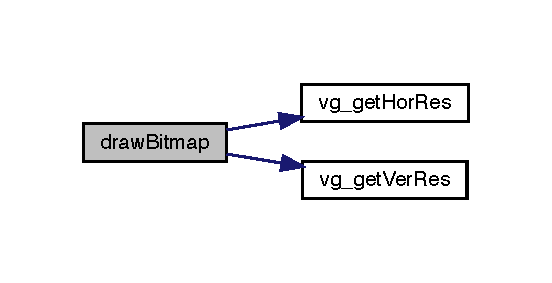
\includegraphics[width=265pt]{group___bitmap_ga82a8171067b55f72cc29c8c50d8330c6_cgraph}
\end{center}
\end{figure}
\hypertarget{group___bitmap_ga3506880ffd407c36eb8aaddd2c1606d2}{}\label{group___bitmap_ga3506880ffd407c36eb8aaddd2c1606d2} 
\index{Bitmap@{Bitmap}!load\+Bitmap@{load\+Bitmap}}
\index{load\+Bitmap@{load\+Bitmap}!Bitmap@{Bitmap}}
\subsubsection{\texorpdfstring{load\+Bitmap()}{loadBitmap()}}
{\footnotesize\ttfamily \hyperlink{struct_bitmap}{Bitmap}$\ast$ load\+Bitmap (\begin{DoxyParamCaption}\item[{const char $\ast$}]{filename }\end{DoxyParamCaption})}



Loads a bmp image. 


\begin{DoxyParams}{Parameters}
{\em filename} & Path of the image to load \\
\hline
\end{DoxyParams}
\begin{DoxyReturn}{Returns}
Non N\+U\+LL pointer to the image buffer 
\end{DoxyReturn}

\hypertarget{group___b_m_ps_holder}{}\section{B\+M\+Ps\+Holder}
\label{group___b_m_ps_holder}\index{B\+M\+Ps\+Holder@{B\+M\+Ps\+Holder}}
\subsection*{Classes}
\begin{DoxyCompactItemize}
\item 
struct \hyperlink{struct_b_m_ps_holder__t}{B\+M\+Ps\+Holder\+\_\+t}
\begin{DoxyCompactList}\small\item\em A structure created to hold all the Bitmaps used in the game. \end{DoxyCompactList}\end{DoxyCompactItemize}
\subsection*{Macros}
\begin{DoxyCompactItemize}
\item 
\#define \hyperlink{group___b_m_ps_holder_ga8cbb8366563bf839a123c77c9dce4654}{N\+U\+M\+\_\+\+E\+X\+P\+L\+O\+S\+I\+O\+N\+\_\+\+B\+M\+PS}~16
\begin{DoxyCompactList}\small\item\em Number of Bitmaps in explosion animation. \end{DoxyCompactList}\item 
\#define \hyperlink{group___b_m_ps_holder_ga879ee79215c5f7b42458ebd3e9258d9a}{N\+U\+M\+\_\+\+B\+U\+I\+L\+D\+I\+N\+G\+S\+\_\+\+B\+M\+PS}~3
\begin{DoxyCompactList}\small\item\em Number of Bitmaps in Buildings destruction Animation. \end{DoxyCompactList}\item 
\#define \hyperlink{group___b_m_ps_holder_ga004574e130b898860d0098ccc3a1a924}{N\+U\+M\+\_\+\+N\+U\+M\+B\+E\+R\+S\+\_\+\+B\+M\+PS}~10
\begin{DoxyCompactList}\small\item\em Number of Bitmaps for the numbers graphic representation. \end{DoxyCompactList}\item 
\#define \hyperlink{group___b_m_ps_holder_ga05fea38384e3b8729c157fb3370d6c91}{E\+X\+P\+L\+O\+S\+I\+O\+N\+\_\+\+S\+I\+Z\+E\+\_\+X}~64
\begin{DoxyCompactList}\small\item\em Visual space occupied by explosions in the horizontal axis. \end{DoxyCompactList}\item 
\#define \hyperlink{group___b_m_ps_holder_ga0eb35331668d32bc55b98c41006da26d}{E\+X\+P\+L\+O\+S\+I\+O\+N\+\_\+\+S\+I\+Z\+E\+\_\+Y}~64
\begin{DoxyCompactList}\small\item\em Visual space occupied by explosions in the vertical axis. \end{DoxyCompactList}\item 
\#define \hyperlink{group___b_m_ps_holder_gaabac832414071a82ad7b568988fe6a68}{N\+U\+M\+B\+E\+R\+\_\+\+S\+I\+Z\+E\+\_\+X}~30
\begin{DoxyCompactList}\small\item\em Visual space occupied by a number in the horizontal axis. \end{DoxyCompactList}\item 
\#define \hyperlink{group___b_m_ps_holder_gad70760092071deb462db0dc776795028}{N\+U\+M\+B\+E\+R\+\_\+\+S\+I\+Z\+E\+\_\+Y}~45
\begin{DoxyCompactList}\small\item\em Visual space occupied by a number in the vertical axis. \end{DoxyCompactList}\item 
\#define \hyperlink{group___b_m_ps_holder_gaf100aba6100fd8859da0ec78d1e8060f}{B\+I\+G\+\_\+\+N\+U\+M\+B\+E\+R\+\_\+\+S\+I\+Z\+E\+\_\+X}~68
\begin{DoxyCompactList}\small\item\em Visual space occupied by a big number in the horizontal axis. \end{DoxyCompactList}\item 
\#define \hyperlink{group___b_m_ps_holder_ga842fcaf13f4ff9ffef8a2cdbd78d3924}{B\+I\+G\+\_\+\+N\+U\+M\+B\+E\+R\+\_\+\+S\+I\+Z\+E\+\_\+Y}~102
\begin{DoxyCompactList}\small\item\em Visual space occupied by a big number in the vertical axis. \end{DoxyCompactList}\item 
\#define \hyperlink{group___b_m_ps_holder_ga55978cc77704142c71897311f71d7029}{B\+U\+I\+L\+D\+I\+N\+G\+\_\+\+S\+I\+Z\+E\+\_\+X}~160
\begin{DoxyCompactList}\small\item\em Visual space occupied by a building in the horizontal axis. \end{DoxyCompactList}\item 
\#define \hyperlink{group___b_m_ps_holder_gadeef9f42a1337cc1b6bb5748b3a34e59}{B\+U\+I\+L\+D\+I\+N\+G0\+\_\+\+S\+I\+Z\+E\+\_\+Y}~16
\begin{DoxyCompactList}\small\item\em Visual space occupied by a destroyed building in the vertical axis. \end{DoxyCompactList}\item 
\#define \hyperlink{group___b_m_ps_holder_gafdf1660eb5aa651aab3f7fcae454e7df}{B\+U\+I\+L\+D\+I\+N\+G1\+\_\+\+S\+I\+Z\+E\+\_\+Y}~48
\begin{DoxyCompactList}\small\item\em Visual space occupied by a partially destroyed building in the vertical axis. \end{DoxyCompactList}\item 
\#define \hyperlink{group___b_m_ps_holder_ga79b5fabee93603f59aae8533c5058326}{B\+U\+I\+L\+D\+I\+N\+G2\+\_\+\+S\+I\+Z\+E\+\_\+Y}~76
\begin{DoxyCompactList}\small\item\em Visual space occupied by a building in the vertical axis. \end{DoxyCompactList}\item 
\#define \hyperlink{group___b_m_ps_holder_ga40c389b30cd50f3fa1dbcb7a6b3546b4}{B\+U\+I\+L\+D\+I\+N\+G\+\_\+\+S\+I\+Z\+E\+\_\+Y}~76
\begin{DoxyCompactList}\small\item\em Visual space occupied by a building in the vertical axis. \end{DoxyCompactList}\item 
\#define \hyperlink{group___b_m_ps_holder_gae4bece6dba12dec287829c15c2f112a1}{H\+E\+A\+R\+T\+\_\+\+S\+I\+Z\+E\+\_\+X}~48
\begin{DoxyCompactList}\small\item\em Visual space occupied by a heart in the horizontal axis. \end{DoxyCompactList}\item 
\#define \hyperlink{group___b_m_ps_holder_ga4353bbd4b002c88bdd587991a9a3a2ce}{H\+E\+A\+R\+T\+\_\+\+S\+I\+Z\+E\+\_\+Y}~48
\begin{DoxyCompactList}\small\item\em Visual space occupied by a heart in the vertical axis. \end{DoxyCompactList}\item 
\#define \hyperlink{group___b_m_ps_holder_gac6a06e6bc22a5b60c419594300c1749f}{C\+A\+N\+N\+O\+N\+\_\+\+S\+I\+Z\+E\+\_\+X}~50
\begin{DoxyCompactList}\small\item\em Visual space occupied by a missile launcher in the horizontal axis. \end{DoxyCompactList}\item 
\#define \hyperlink{group___b_m_ps_holder_gad3b9eb80fe60bc8f7530633439fa9b25}{C\+A\+N\+N\+O\+N\+\_\+\+S\+I\+Z\+E\+\_\+Y}~62
\begin{DoxyCompactList}\small\item\em Visual space occupied by a missile launcher in the vertical axis. \end{DoxyCompactList}\item 
\#define \hyperlink{group___b_m_ps_holder_ga3d387db7d44e83471b3a63d94ab7a5b9}{B\+U\+T\+T\+O\+N\+S\+\_\+X}~211
\begin{DoxyCompactList}\small\item\em Initial position of menu buttons in the horizontal axis. \end{DoxyCompactList}\item 
\#define \hyperlink{group___b_m_ps_holder_ga19da38bd34116364d23ed824fbede542}{S\+I\+N\+G\+L\+E\+P\+\_\+Y}~231
\begin{DoxyCompactList}\small\item\em Initial position of single player button in the vertical axis. \end{DoxyCompactList}\item 
\#define \hyperlink{group___b_m_ps_holder_ga1d957cbc192cbdb76c80729a7a4e8781}{M\+U\+L\+T\+I\+P\+\_\+Y}~334
\begin{DoxyCompactList}\small\item\em Initial position of multi player button in the vertical axis. \end{DoxyCompactList}\item 
\#define \hyperlink{group___b_m_ps_holder_gac1e57f1ff5614ef7f370bcc296db9bb7}{H\+I\+G\+H\+S\+\_\+Y}~445
\begin{DoxyCompactList}\small\item\em Initial position of highscores button in the vertical axis. \end{DoxyCompactList}\item 
\#define \hyperlink{group___b_m_ps_holder_gabdf8cdcc51fec3510df544a673532eaa}{B\+U\+T\+T\+O\+N\+S\+\_\+\+W\+I\+D\+TH}~376
\begin{DoxyCompactList}\small\item\em Width of the menu buttons. \end{DoxyCompactList}\item 
\#define \hyperlink{group___b_m_ps_holder_ga9721e4c146c7397fb06134ef6716d19b}{B\+U\+T\+T\+O\+N\+S\+\_\+\+H\+E\+I\+G\+HT}~82
\begin{DoxyCompactList}\small\item\em Height of the menu buttons. \end{DoxyCompactList}\item 
\#define \hyperlink{group___b_m_ps_holder_gaefbb305e5b4d7c7402d158fff6f1c163}{E\+X\+I\+T\+\_\+X}~759
\begin{DoxyCompactList}\small\item\em Center position of exit button in the horizontal axis. \end{DoxyCompactList}\item 
\#define \hyperlink{group___b_m_ps_holder_ga46bb001d1c62f7725f3258824caeb260}{E\+X\+I\+T\+\_\+Y}~566
\begin{DoxyCompactList}\small\item\em Center position of exit button in the vertical axis. \end{DoxyCompactList}\item 
\#define \hyperlink{group___b_m_ps_holder_ga7c73a85659bf774239d3897ab04e68de}{E\+X\+I\+T\+\_\+\+R\+A\+D\+I\+US}~17
\begin{DoxyCompactList}\small\item\em Radius of the circle representing the exit button. \end{DoxyCompactList}\item 
\#define \hyperlink{group___b_m_ps_holder_gaaa856bb92cc9efc1e6cffeee78fe19b6}{H\+I\+G\+H\+S\+C\+O\+R\+E\+\_\+\+S\+I\+Z\+E\+\_\+X}~410
\begin{DoxyCompactList}\small\item\em Visual space occupied by the highscore text in the horizontal axis. \end{DoxyCompactList}\item 
\#define \hyperlink{group___b_m_ps_holder_ga58bb49ecfe4e566c5c282e55faa900dc}{H\+I\+G\+H\+S\+C\+O\+R\+E\+\_\+\+S\+I\+Z\+E\+\_\+Y}~50
\begin{DoxyCompactList}\small\item\em Visual space occupied by the highscore text in the vertical axis. \end{DoxyCompactList}\end{DoxyCompactItemize}
\subsection*{Functions}
\begin{DoxyCompactItemize}
\item 
\hyperlink{struct_b_m_ps_holder__t}{B\+M\+Ps\+Holder\+\_\+t} $\ast$ \hyperlink{group___b_m_ps_holder_gafd662085ea52a83586cddd30b6423c01}{B\+M\+Ps\+Holder} ()
\item 
void \hyperlink{group___b_m_ps_holder_gaa0a362e75eb034aa78e675ecb1b9c6da}{delete\+\_\+bmps\+\_\+holder} ()
\item 
\hyperlink{struct_bitmap}{Bitmap} $\ast$$\ast$ \hyperlink{group___b_m_ps_holder_gab74a07b3201edddc82762946608675a5}{load\+\_\+bmps} (const char $\ast$base, unsigned num)
\item 
void \hyperlink{group___b_m_ps_holder_ga72dfdb9916627f68651174c037680533}{delete\+\_\+bmps} (\hyperlink{struct_bitmap}{Bitmap} $\ast$$\ast$arr, unsigned num)
\end{DoxyCompactItemize}


\subsection{Detailed Description}
Functions for manipulating a structure holding Bitmaps. 

\subsection{Macro Definition Documentation}
\hypertarget{group___b_m_ps_holder_gaf100aba6100fd8859da0ec78d1e8060f}{}\label{group___b_m_ps_holder_gaf100aba6100fd8859da0ec78d1e8060f} 
\index{B\+M\+Ps\+Holder@{B\+M\+Ps\+Holder}!B\+I\+G\+\_\+\+N\+U\+M\+B\+E\+R\+\_\+\+S\+I\+Z\+E\+\_\+X@{B\+I\+G\+\_\+\+N\+U\+M\+B\+E\+R\+\_\+\+S\+I\+Z\+E\+\_\+X}}
\index{B\+I\+G\+\_\+\+N\+U\+M\+B\+E\+R\+\_\+\+S\+I\+Z\+E\+\_\+X@{B\+I\+G\+\_\+\+N\+U\+M\+B\+E\+R\+\_\+\+S\+I\+Z\+E\+\_\+X}!B\+M\+Ps\+Holder@{B\+M\+Ps\+Holder}}
\subsubsection{\texorpdfstring{B\+I\+G\+\_\+\+N\+U\+M\+B\+E\+R\+\_\+\+S\+I\+Z\+E\+\_\+X}{BIG\_NUMBER\_SIZE\_X}}
{\footnotesize\ttfamily \#define B\+I\+G\+\_\+\+N\+U\+M\+B\+E\+R\+\_\+\+S\+I\+Z\+E\+\_\+X~68}



Visual space occupied by a big number in the horizontal axis. 

\hypertarget{group___b_m_ps_holder_ga842fcaf13f4ff9ffef8a2cdbd78d3924}{}\label{group___b_m_ps_holder_ga842fcaf13f4ff9ffef8a2cdbd78d3924} 
\index{B\+M\+Ps\+Holder@{B\+M\+Ps\+Holder}!B\+I\+G\+\_\+\+N\+U\+M\+B\+E\+R\+\_\+\+S\+I\+Z\+E\+\_\+Y@{B\+I\+G\+\_\+\+N\+U\+M\+B\+E\+R\+\_\+\+S\+I\+Z\+E\+\_\+Y}}
\index{B\+I\+G\+\_\+\+N\+U\+M\+B\+E\+R\+\_\+\+S\+I\+Z\+E\+\_\+Y@{B\+I\+G\+\_\+\+N\+U\+M\+B\+E\+R\+\_\+\+S\+I\+Z\+E\+\_\+Y}!B\+M\+Ps\+Holder@{B\+M\+Ps\+Holder}}
\subsubsection{\texorpdfstring{B\+I\+G\+\_\+\+N\+U\+M\+B\+E\+R\+\_\+\+S\+I\+Z\+E\+\_\+Y}{BIG\_NUMBER\_SIZE\_Y}}
{\footnotesize\ttfamily \#define B\+I\+G\+\_\+\+N\+U\+M\+B\+E\+R\+\_\+\+S\+I\+Z\+E\+\_\+Y~102}



Visual space occupied by a big number in the vertical axis. 

\hypertarget{group___b_m_ps_holder_gadeef9f42a1337cc1b6bb5748b3a34e59}{}\label{group___b_m_ps_holder_gadeef9f42a1337cc1b6bb5748b3a34e59} 
\index{B\+M\+Ps\+Holder@{B\+M\+Ps\+Holder}!B\+U\+I\+L\+D\+I\+N\+G0\+\_\+\+S\+I\+Z\+E\+\_\+Y@{B\+U\+I\+L\+D\+I\+N\+G0\+\_\+\+S\+I\+Z\+E\+\_\+Y}}
\index{B\+U\+I\+L\+D\+I\+N\+G0\+\_\+\+S\+I\+Z\+E\+\_\+Y@{B\+U\+I\+L\+D\+I\+N\+G0\+\_\+\+S\+I\+Z\+E\+\_\+Y}!B\+M\+Ps\+Holder@{B\+M\+Ps\+Holder}}
\subsubsection{\texorpdfstring{B\+U\+I\+L\+D\+I\+N\+G0\+\_\+\+S\+I\+Z\+E\+\_\+Y}{BUILDING0\_SIZE\_Y}}
{\footnotesize\ttfamily \#define B\+U\+I\+L\+D\+I\+N\+G0\+\_\+\+S\+I\+Z\+E\+\_\+Y~16}



Visual space occupied by a destroyed building in the vertical axis. 

\hypertarget{group___b_m_ps_holder_gafdf1660eb5aa651aab3f7fcae454e7df}{}\label{group___b_m_ps_holder_gafdf1660eb5aa651aab3f7fcae454e7df} 
\index{B\+M\+Ps\+Holder@{B\+M\+Ps\+Holder}!B\+U\+I\+L\+D\+I\+N\+G1\+\_\+\+S\+I\+Z\+E\+\_\+Y@{B\+U\+I\+L\+D\+I\+N\+G1\+\_\+\+S\+I\+Z\+E\+\_\+Y}}
\index{B\+U\+I\+L\+D\+I\+N\+G1\+\_\+\+S\+I\+Z\+E\+\_\+Y@{B\+U\+I\+L\+D\+I\+N\+G1\+\_\+\+S\+I\+Z\+E\+\_\+Y}!B\+M\+Ps\+Holder@{B\+M\+Ps\+Holder}}
\subsubsection{\texorpdfstring{B\+U\+I\+L\+D\+I\+N\+G1\+\_\+\+S\+I\+Z\+E\+\_\+Y}{BUILDING1\_SIZE\_Y}}
{\footnotesize\ttfamily \#define B\+U\+I\+L\+D\+I\+N\+G1\+\_\+\+S\+I\+Z\+E\+\_\+Y~48}



Visual space occupied by a partially destroyed building in the vertical axis. 

\hypertarget{group___b_m_ps_holder_ga79b5fabee93603f59aae8533c5058326}{}\label{group___b_m_ps_holder_ga79b5fabee93603f59aae8533c5058326} 
\index{B\+M\+Ps\+Holder@{B\+M\+Ps\+Holder}!B\+U\+I\+L\+D\+I\+N\+G2\+\_\+\+S\+I\+Z\+E\+\_\+Y@{B\+U\+I\+L\+D\+I\+N\+G2\+\_\+\+S\+I\+Z\+E\+\_\+Y}}
\index{B\+U\+I\+L\+D\+I\+N\+G2\+\_\+\+S\+I\+Z\+E\+\_\+Y@{B\+U\+I\+L\+D\+I\+N\+G2\+\_\+\+S\+I\+Z\+E\+\_\+Y}!B\+M\+Ps\+Holder@{B\+M\+Ps\+Holder}}
\subsubsection{\texorpdfstring{B\+U\+I\+L\+D\+I\+N\+G2\+\_\+\+S\+I\+Z\+E\+\_\+Y}{BUILDING2\_SIZE\_Y}}
{\footnotesize\ttfamily \#define B\+U\+I\+L\+D\+I\+N\+G2\+\_\+\+S\+I\+Z\+E\+\_\+Y~76}



Visual space occupied by a building in the vertical axis. 

\hypertarget{group___b_m_ps_holder_ga55978cc77704142c71897311f71d7029}{}\label{group___b_m_ps_holder_ga55978cc77704142c71897311f71d7029} 
\index{B\+M\+Ps\+Holder@{B\+M\+Ps\+Holder}!B\+U\+I\+L\+D\+I\+N\+G\+\_\+\+S\+I\+Z\+E\+\_\+X@{B\+U\+I\+L\+D\+I\+N\+G\+\_\+\+S\+I\+Z\+E\+\_\+X}}
\index{B\+U\+I\+L\+D\+I\+N\+G\+\_\+\+S\+I\+Z\+E\+\_\+X@{B\+U\+I\+L\+D\+I\+N\+G\+\_\+\+S\+I\+Z\+E\+\_\+X}!B\+M\+Ps\+Holder@{B\+M\+Ps\+Holder}}
\subsubsection{\texorpdfstring{B\+U\+I\+L\+D\+I\+N\+G\+\_\+\+S\+I\+Z\+E\+\_\+X}{BUILDING\_SIZE\_X}}
{\footnotesize\ttfamily \#define B\+U\+I\+L\+D\+I\+N\+G\+\_\+\+S\+I\+Z\+E\+\_\+X~160}



Visual space occupied by a building in the horizontal axis. 

\hypertarget{group___b_m_ps_holder_ga40c389b30cd50f3fa1dbcb7a6b3546b4}{}\label{group___b_m_ps_holder_ga40c389b30cd50f3fa1dbcb7a6b3546b4} 
\index{B\+M\+Ps\+Holder@{B\+M\+Ps\+Holder}!B\+U\+I\+L\+D\+I\+N\+G\+\_\+\+S\+I\+Z\+E\+\_\+Y@{B\+U\+I\+L\+D\+I\+N\+G\+\_\+\+S\+I\+Z\+E\+\_\+Y}}
\index{B\+U\+I\+L\+D\+I\+N\+G\+\_\+\+S\+I\+Z\+E\+\_\+Y@{B\+U\+I\+L\+D\+I\+N\+G\+\_\+\+S\+I\+Z\+E\+\_\+Y}!B\+M\+Ps\+Holder@{B\+M\+Ps\+Holder}}
\subsubsection{\texorpdfstring{B\+U\+I\+L\+D\+I\+N\+G\+\_\+\+S\+I\+Z\+E\+\_\+Y}{BUILDING\_SIZE\_Y}}
{\footnotesize\ttfamily \#define B\+U\+I\+L\+D\+I\+N\+G\+\_\+\+S\+I\+Z\+E\+\_\+Y~76}



Visual space occupied by a building in the vertical axis. 

\hypertarget{group___b_m_ps_holder_ga9721e4c146c7397fb06134ef6716d19b}{}\label{group___b_m_ps_holder_ga9721e4c146c7397fb06134ef6716d19b} 
\index{B\+M\+Ps\+Holder@{B\+M\+Ps\+Holder}!B\+U\+T\+T\+O\+N\+S\+\_\+\+H\+E\+I\+G\+HT@{B\+U\+T\+T\+O\+N\+S\+\_\+\+H\+E\+I\+G\+HT}}
\index{B\+U\+T\+T\+O\+N\+S\+\_\+\+H\+E\+I\+G\+HT@{B\+U\+T\+T\+O\+N\+S\+\_\+\+H\+E\+I\+G\+HT}!B\+M\+Ps\+Holder@{B\+M\+Ps\+Holder}}
\subsubsection{\texorpdfstring{B\+U\+T\+T\+O\+N\+S\+\_\+\+H\+E\+I\+G\+HT}{BUTTONS\_HEIGHT}}
{\footnotesize\ttfamily \#define B\+U\+T\+T\+O\+N\+S\+\_\+\+H\+E\+I\+G\+HT~82}



Height of the menu buttons. 

\hypertarget{group___b_m_ps_holder_gabdf8cdcc51fec3510df544a673532eaa}{}\label{group___b_m_ps_holder_gabdf8cdcc51fec3510df544a673532eaa} 
\index{B\+M\+Ps\+Holder@{B\+M\+Ps\+Holder}!B\+U\+T\+T\+O\+N\+S\+\_\+\+W\+I\+D\+TH@{B\+U\+T\+T\+O\+N\+S\+\_\+\+W\+I\+D\+TH}}
\index{B\+U\+T\+T\+O\+N\+S\+\_\+\+W\+I\+D\+TH@{B\+U\+T\+T\+O\+N\+S\+\_\+\+W\+I\+D\+TH}!B\+M\+Ps\+Holder@{B\+M\+Ps\+Holder}}
\subsubsection{\texorpdfstring{B\+U\+T\+T\+O\+N\+S\+\_\+\+W\+I\+D\+TH}{BUTTONS\_WIDTH}}
{\footnotesize\ttfamily \#define B\+U\+T\+T\+O\+N\+S\+\_\+\+W\+I\+D\+TH~376}



Width of the menu buttons. 

\hypertarget{group___b_m_ps_holder_ga3d387db7d44e83471b3a63d94ab7a5b9}{}\label{group___b_m_ps_holder_ga3d387db7d44e83471b3a63d94ab7a5b9} 
\index{B\+M\+Ps\+Holder@{B\+M\+Ps\+Holder}!B\+U\+T\+T\+O\+N\+S\+\_\+X@{B\+U\+T\+T\+O\+N\+S\+\_\+X}}
\index{B\+U\+T\+T\+O\+N\+S\+\_\+X@{B\+U\+T\+T\+O\+N\+S\+\_\+X}!B\+M\+Ps\+Holder@{B\+M\+Ps\+Holder}}
\subsubsection{\texorpdfstring{B\+U\+T\+T\+O\+N\+S\+\_\+X}{BUTTONS\_X}}
{\footnotesize\ttfamily \#define B\+U\+T\+T\+O\+N\+S\+\_\+X~211}



Initial position of menu buttons in the horizontal axis. 

\hypertarget{group___b_m_ps_holder_gac6a06e6bc22a5b60c419594300c1749f}{}\label{group___b_m_ps_holder_gac6a06e6bc22a5b60c419594300c1749f} 
\index{B\+M\+Ps\+Holder@{B\+M\+Ps\+Holder}!C\+A\+N\+N\+O\+N\+\_\+\+S\+I\+Z\+E\+\_\+X@{C\+A\+N\+N\+O\+N\+\_\+\+S\+I\+Z\+E\+\_\+X}}
\index{C\+A\+N\+N\+O\+N\+\_\+\+S\+I\+Z\+E\+\_\+X@{C\+A\+N\+N\+O\+N\+\_\+\+S\+I\+Z\+E\+\_\+X}!B\+M\+Ps\+Holder@{B\+M\+Ps\+Holder}}
\subsubsection{\texorpdfstring{C\+A\+N\+N\+O\+N\+\_\+\+S\+I\+Z\+E\+\_\+X}{CANNON\_SIZE\_X}}
{\footnotesize\ttfamily \#define C\+A\+N\+N\+O\+N\+\_\+\+S\+I\+Z\+E\+\_\+X~50}



Visual space occupied by a missile launcher in the horizontal axis. 

\hypertarget{group___b_m_ps_holder_gad3b9eb80fe60bc8f7530633439fa9b25}{}\label{group___b_m_ps_holder_gad3b9eb80fe60bc8f7530633439fa9b25} 
\index{B\+M\+Ps\+Holder@{B\+M\+Ps\+Holder}!C\+A\+N\+N\+O\+N\+\_\+\+S\+I\+Z\+E\+\_\+Y@{C\+A\+N\+N\+O\+N\+\_\+\+S\+I\+Z\+E\+\_\+Y}}
\index{C\+A\+N\+N\+O\+N\+\_\+\+S\+I\+Z\+E\+\_\+Y@{C\+A\+N\+N\+O\+N\+\_\+\+S\+I\+Z\+E\+\_\+Y}!B\+M\+Ps\+Holder@{B\+M\+Ps\+Holder}}
\subsubsection{\texorpdfstring{C\+A\+N\+N\+O\+N\+\_\+\+S\+I\+Z\+E\+\_\+Y}{CANNON\_SIZE\_Y}}
{\footnotesize\ttfamily \#define C\+A\+N\+N\+O\+N\+\_\+\+S\+I\+Z\+E\+\_\+Y~62}



Visual space occupied by a missile launcher in the vertical axis. 

\hypertarget{group___b_m_ps_holder_ga7c73a85659bf774239d3897ab04e68de}{}\label{group___b_m_ps_holder_ga7c73a85659bf774239d3897ab04e68de} 
\index{B\+M\+Ps\+Holder@{B\+M\+Ps\+Holder}!E\+X\+I\+T\+\_\+\+R\+A\+D\+I\+US@{E\+X\+I\+T\+\_\+\+R\+A\+D\+I\+US}}
\index{E\+X\+I\+T\+\_\+\+R\+A\+D\+I\+US@{E\+X\+I\+T\+\_\+\+R\+A\+D\+I\+US}!B\+M\+Ps\+Holder@{B\+M\+Ps\+Holder}}
\subsubsection{\texorpdfstring{E\+X\+I\+T\+\_\+\+R\+A\+D\+I\+US}{EXIT\_RADIUS}}
{\footnotesize\ttfamily \#define E\+X\+I\+T\+\_\+\+R\+A\+D\+I\+US~17}



Radius of the circle representing the exit button. 

\hypertarget{group___b_m_ps_holder_gaefbb305e5b4d7c7402d158fff6f1c163}{}\label{group___b_m_ps_holder_gaefbb305e5b4d7c7402d158fff6f1c163} 
\index{B\+M\+Ps\+Holder@{B\+M\+Ps\+Holder}!E\+X\+I\+T\+\_\+X@{E\+X\+I\+T\+\_\+X}}
\index{E\+X\+I\+T\+\_\+X@{E\+X\+I\+T\+\_\+X}!B\+M\+Ps\+Holder@{B\+M\+Ps\+Holder}}
\subsubsection{\texorpdfstring{E\+X\+I\+T\+\_\+X}{EXIT\_X}}
{\footnotesize\ttfamily \#define E\+X\+I\+T\+\_\+X~759}



Center position of exit button in the horizontal axis. 

\hypertarget{group___b_m_ps_holder_ga46bb001d1c62f7725f3258824caeb260}{}\label{group___b_m_ps_holder_ga46bb001d1c62f7725f3258824caeb260} 
\index{B\+M\+Ps\+Holder@{B\+M\+Ps\+Holder}!E\+X\+I\+T\+\_\+Y@{E\+X\+I\+T\+\_\+Y}}
\index{E\+X\+I\+T\+\_\+Y@{E\+X\+I\+T\+\_\+Y}!B\+M\+Ps\+Holder@{B\+M\+Ps\+Holder}}
\subsubsection{\texorpdfstring{E\+X\+I\+T\+\_\+Y}{EXIT\_Y}}
{\footnotesize\ttfamily \#define E\+X\+I\+T\+\_\+Y~566}



Center position of exit button in the vertical axis. 

\hypertarget{group___b_m_ps_holder_ga05fea38384e3b8729c157fb3370d6c91}{}\label{group___b_m_ps_holder_ga05fea38384e3b8729c157fb3370d6c91} 
\index{B\+M\+Ps\+Holder@{B\+M\+Ps\+Holder}!E\+X\+P\+L\+O\+S\+I\+O\+N\+\_\+\+S\+I\+Z\+E\+\_\+X@{E\+X\+P\+L\+O\+S\+I\+O\+N\+\_\+\+S\+I\+Z\+E\+\_\+X}}
\index{E\+X\+P\+L\+O\+S\+I\+O\+N\+\_\+\+S\+I\+Z\+E\+\_\+X@{E\+X\+P\+L\+O\+S\+I\+O\+N\+\_\+\+S\+I\+Z\+E\+\_\+X}!B\+M\+Ps\+Holder@{B\+M\+Ps\+Holder}}
\subsubsection{\texorpdfstring{E\+X\+P\+L\+O\+S\+I\+O\+N\+\_\+\+S\+I\+Z\+E\+\_\+X}{EXPLOSION\_SIZE\_X}}
{\footnotesize\ttfamily \#define E\+X\+P\+L\+O\+S\+I\+O\+N\+\_\+\+S\+I\+Z\+E\+\_\+X~64}



Visual space occupied by explosions in the horizontal axis. 

\hypertarget{group___b_m_ps_holder_ga0eb35331668d32bc55b98c41006da26d}{}\label{group___b_m_ps_holder_ga0eb35331668d32bc55b98c41006da26d} 
\index{B\+M\+Ps\+Holder@{B\+M\+Ps\+Holder}!E\+X\+P\+L\+O\+S\+I\+O\+N\+\_\+\+S\+I\+Z\+E\+\_\+Y@{E\+X\+P\+L\+O\+S\+I\+O\+N\+\_\+\+S\+I\+Z\+E\+\_\+Y}}
\index{E\+X\+P\+L\+O\+S\+I\+O\+N\+\_\+\+S\+I\+Z\+E\+\_\+Y@{E\+X\+P\+L\+O\+S\+I\+O\+N\+\_\+\+S\+I\+Z\+E\+\_\+Y}!B\+M\+Ps\+Holder@{B\+M\+Ps\+Holder}}
\subsubsection{\texorpdfstring{E\+X\+P\+L\+O\+S\+I\+O\+N\+\_\+\+S\+I\+Z\+E\+\_\+Y}{EXPLOSION\_SIZE\_Y}}
{\footnotesize\ttfamily \#define E\+X\+P\+L\+O\+S\+I\+O\+N\+\_\+\+S\+I\+Z\+E\+\_\+Y~64}



Visual space occupied by explosions in the vertical axis. 

\hypertarget{group___b_m_ps_holder_gae4bece6dba12dec287829c15c2f112a1}{}\label{group___b_m_ps_holder_gae4bece6dba12dec287829c15c2f112a1} 
\index{B\+M\+Ps\+Holder@{B\+M\+Ps\+Holder}!H\+E\+A\+R\+T\+\_\+\+S\+I\+Z\+E\+\_\+X@{H\+E\+A\+R\+T\+\_\+\+S\+I\+Z\+E\+\_\+X}}
\index{H\+E\+A\+R\+T\+\_\+\+S\+I\+Z\+E\+\_\+X@{H\+E\+A\+R\+T\+\_\+\+S\+I\+Z\+E\+\_\+X}!B\+M\+Ps\+Holder@{B\+M\+Ps\+Holder}}
\subsubsection{\texorpdfstring{H\+E\+A\+R\+T\+\_\+\+S\+I\+Z\+E\+\_\+X}{HEART\_SIZE\_X}}
{\footnotesize\ttfamily \#define H\+E\+A\+R\+T\+\_\+\+S\+I\+Z\+E\+\_\+X~48}



Visual space occupied by a heart in the horizontal axis. 

\hypertarget{group___b_m_ps_holder_ga4353bbd4b002c88bdd587991a9a3a2ce}{}\label{group___b_m_ps_holder_ga4353bbd4b002c88bdd587991a9a3a2ce} 
\index{B\+M\+Ps\+Holder@{B\+M\+Ps\+Holder}!H\+E\+A\+R\+T\+\_\+\+S\+I\+Z\+E\+\_\+Y@{H\+E\+A\+R\+T\+\_\+\+S\+I\+Z\+E\+\_\+Y}}
\index{H\+E\+A\+R\+T\+\_\+\+S\+I\+Z\+E\+\_\+Y@{H\+E\+A\+R\+T\+\_\+\+S\+I\+Z\+E\+\_\+Y}!B\+M\+Ps\+Holder@{B\+M\+Ps\+Holder}}
\subsubsection{\texorpdfstring{H\+E\+A\+R\+T\+\_\+\+S\+I\+Z\+E\+\_\+Y}{HEART\_SIZE\_Y}}
{\footnotesize\ttfamily \#define H\+E\+A\+R\+T\+\_\+\+S\+I\+Z\+E\+\_\+Y~48}



Visual space occupied by a heart in the vertical axis. 

\hypertarget{group___b_m_ps_holder_gac1e57f1ff5614ef7f370bcc296db9bb7}{}\label{group___b_m_ps_holder_gac1e57f1ff5614ef7f370bcc296db9bb7} 
\index{B\+M\+Ps\+Holder@{B\+M\+Ps\+Holder}!H\+I\+G\+H\+S\+\_\+Y@{H\+I\+G\+H\+S\+\_\+Y}}
\index{H\+I\+G\+H\+S\+\_\+Y@{H\+I\+G\+H\+S\+\_\+Y}!B\+M\+Ps\+Holder@{B\+M\+Ps\+Holder}}
\subsubsection{\texorpdfstring{H\+I\+G\+H\+S\+\_\+Y}{HIGHS\_Y}}
{\footnotesize\ttfamily \#define H\+I\+G\+H\+S\+\_\+Y~445}



Initial position of highscores button in the vertical axis. 

\hypertarget{group___b_m_ps_holder_gaaa856bb92cc9efc1e6cffeee78fe19b6}{}\label{group___b_m_ps_holder_gaaa856bb92cc9efc1e6cffeee78fe19b6} 
\index{B\+M\+Ps\+Holder@{B\+M\+Ps\+Holder}!H\+I\+G\+H\+S\+C\+O\+R\+E\+\_\+\+S\+I\+Z\+E\+\_\+X@{H\+I\+G\+H\+S\+C\+O\+R\+E\+\_\+\+S\+I\+Z\+E\+\_\+X}}
\index{H\+I\+G\+H\+S\+C\+O\+R\+E\+\_\+\+S\+I\+Z\+E\+\_\+X@{H\+I\+G\+H\+S\+C\+O\+R\+E\+\_\+\+S\+I\+Z\+E\+\_\+X}!B\+M\+Ps\+Holder@{B\+M\+Ps\+Holder}}
\subsubsection{\texorpdfstring{H\+I\+G\+H\+S\+C\+O\+R\+E\+\_\+\+S\+I\+Z\+E\+\_\+X}{HIGHSCORE\_SIZE\_X}}
{\footnotesize\ttfamily \#define H\+I\+G\+H\+S\+C\+O\+R\+E\+\_\+\+S\+I\+Z\+E\+\_\+X~410}



Visual space occupied by the highscore text in the horizontal axis. 

\hypertarget{group___b_m_ps_holder_ga58bb49ecfe4e566c5c282e55faa900dc}{}\label{group___b_m_ps_holder_ga58bb49ecfe4e566c5c282e55faa900dc} 
\index{B\+M\+Ps\+Holder@{B\+M\+Ps\+Holder}!H\+I\+G\+H\+S\+C\+O\+R\+E\+\_\+\+S\+I\+Z\+E\+\_\+Y@{H\+I\+G\+H\+S\+C\+O\+R\+E\+\_\+\+S\+I\+Z\+E\+\_\+Y}}
\index{H\+I\+G\+H\+S\+C\+O\+R\+E\+\_\+\+S\+I\+Z\+E\+\_\+Y@{H\+I\+G\+H\+S\+C\+O\+R\+E\+\_\+\+S\+I\+Z\+E\+\_\+Y}!B\+M\+Ps\+Holder@{B\+M\+Ps\+Holder}}
\subsubsection{\texorpdfstring{H\+I\+G\+H\+S\+C\+O\+R\+E\+\_\+\+S\+I\+Z\+E\+\_\+Y}{HIGHSCORE\_SIZE\_Y}}
{\footnotesize\ttfamily \#define H\+I\+G\+H\+S\+C\+O\+R\+E\+\_\+\+S\+I\+Z\+E\+\_\+Y~50}



Visual space occupied by the highscore text in the vertical axis. 

\hypertarget{group___b_m_ps_holder_ga1d957cbc192cbdb76c80729a7a4e8781}{}\label{group___b_m_ps_holder_ga1d957cbc192cbdb76c80729a7a4e8781} 
\index{B\+M\+Ps\+Holder@{B\+M\+Ps\+Holder}!M\+U\+L\+T\+I\+P\+\_\+Y@{M\+U\+L\+T\+I\+P\+\_\+Y}}
\index{M\+U\+L\+T\+I\+P\+\_\+Y@{M\+U\+L\+T\+I\+P\+\_\+Y}!B\+M\+Ps\+Holder@{B\+M\+Ps\+Holder}}
\subsubsection{\texorpdfstring{M\+U\+L\+T\+I\+P\+\_\+Y}{MULTIP\_Y}}
{\footnotesize\ttfamily \#define M\+U\+L\+T\+I\+P\+\_\+Y~334}



Initial position of multi player button in the vertical axis. 

\hypertarget{group___b_m_ps_holder_ga879ee79215c5f7b42458ebd3e9258d9a}{}\label{group___b_m_ps_holder_ga879ee79215c5f7b42458ebd3e9258d9a} 
\index{B\+M\+Ps\+Holder@{B\+M\+Ps\+Holder}!N\+U\+M\+\_\+\+B\+U\+I\+L\+D\+I\+N\+G\+S\+\_\+\+B\+M\+PS@{N\+U\+M\+\_\+\+B\+U\+I\+L\+D\+I\+N\+G\+S\+\_\+\+B\+M\+PS}}
\index{N\+U\+M\+\_\+\+B\+U\+I\+L\+D\+I\+N\+G\+S\+\_\+\+B\+M\+PS@{N\+U\+M\+\_\+\+B\+U\+I\+L\+D\+I\+N\+G\+S\+\_\+\+B\+M\+PS}!B\+M\+Ps\+Holder@{B\+M\+Ps\+Holder}}
\subsubsection{\texorpdfstring{N\+U\+M\+\_\+\+B\+U\+I\+L\+D\+I\+N\+G\+S\+\_\+\+B\+M\+PS}{NUM\_BUILDINGS\_BMPS}}
{\footnotesize\ttfamily \#define N\+U\+M\+\_\+\+B\+U\+I\+L\+D\+I\+N\+G\+S\+\_\+\+B\+M\+PS~3}



Number of Bitmaps in Buildings destruction Animation. 

\hypertarget{group___b_m_ps_holder_ga8cbb8366563bf839a123c77c9dce4654}{}\label{group___b_m_ps_holder_ga8cbb8366563bf839a123c77c9dce4654} 
\index{B\+M\+Ps\+Holder@{B\+M\+Ps\+Holder}!N\+U\+M\+\_\+\+E\+X\+P\+L\+O\+S\+I\+O\+N\+\_\+\+B\+M\+PS@{N\+U\+M\+\_\+\+E\+X\+P\+L\+O\+S\+I\+O\+N\+\_\+\+B\+M\+PS}}
\index{N\+U\+M\+\_\+\+E\+X\+P\+L\+O\+S\+I\+O\+N\+\_\+\+B\+M\+PS@{N\+U\+M\+\_\+\+E\+X\+P\+L\+O\+S\+I\+O\+N\+\_\+\+B\+M\+PS}!B\+M\+Ps\+Holder@{B\+M\+Ps\+Holder}}
\subsubsection{\texorpdfstring{N\+U\+M\+\_\+\+E\+X\+P\+L\+O\+S\+I\+O\+N\+\_\+\+B\+M\+PS}{NUM\_EXPLOSION\_BMPS}}
{\footnotesize\ttfamily \#define N\+U\+M\+\_\+\+E\+X\+P\+L\+O\+S\+I\+O\+N\+\_\+\+B\+M\+PS~16}



Number of Bitmaps in explosion animation. 

\hypertarget{group___b_m_ps_holder_ga004574e130b898860d0098ccc3a1a924}{}\label{group___b_m_ps_holder_ga004574e130b898860d0098ccc3a1a924} 
\index{B\+M\+Ps\+Holder@{B\+M\+Ps\+Holder}!N\+U\+M\+\_\+\+N\+U\+M\+B\+E\+R\+S\+\_\+\+B\+M\+PS@{N\+U\+M\+\_\+\+N\+U\+M\+B\+E\+R\+S\+\_\+\+B\+M\+PS}}
\index{N\+U\+M\+\_\+\+N\+U\+M\+B\+E\+R\+S\+\_\+\+B\+M\+PS@{N\+U\+M\+\_\+\+N\+U\+M\+B\+E\+R\+S\+\_\+\+B\+M\+PS}!B\+M\+Ps\+Holder@{B\+M\+Ps\+Holder}}
\subsubsection{\texorpdfstring{N\+U\+M\+\_\+\+N\+U\+M\+B\+E\+R\+S\+\_\+\+B\+M\+PS}{NUM\_NUMBERS\_BMPS}}
{\footnotesize\ttfamily \#define N\+U\+M\+\_\+\+N\+U\+M\+B\+E\+R\+S\+\_\+\+B\+M\+PS~10}



Number of Bitmaps for the numbers graphic representation. 

\hypertarget{group___b_m_ps_holder_gaabac832414071a82ad7b568988fe6a68}{}\label{group___b_m_ps_holder_gaabac832414071a82ad7b568988fe6a68} 
\index{B\+M\+Ps\+Holder@{B\+M\+Ps\+Holder}!N\+U\+M\+B\+E\+R\+\_\+\+S\+I\+Z\+E\+\_\+X@{N\+U\+M\+B\+E\+R\+\_\+\+S\+I\+Z\+E\+\_\+X}}
\index{N\+U\+M\+B\+E\+R\+\_\+\+S\+I\+Z\+E\+\_\+X@{N\+U\+M\+B\+E\+R\+\_\+\+S\+I\+Z\+E\+\_\+X}!B\+M\+Ps\+Holder@{B\+M\+Ps\+Holder}}
\subsubsection{\texorpdfstring{N\+U\+M\+B\+E\+R\+\_\+\+S\+I\+Z\+E\+\_\+X}{NUMBER\_SIZE\_X}}
{\footnotesize\ttfamily \#define N\+U\+M\+B\+E\+R\+\_\+\+S\+I\+Z\+E\+\_\+X~30}



Visual space occupied by a number in the horizontal axis. 

\hypertarget{group___b_m_ps_holder_gad70760092071deb462db0dc776795028}{}\label{group___b_m_ps_holder_gad70760092071deb462db0dc776795028} 
\index{B\+M\+Ps\+Holder@{B\+M\+Ps\+Holder}!N\+U\+M\+B\+E\+R\+\_\+\+S\+I\+Z\+E\+\_\+Y@{N\+U\+M\+B\+E\+R\+\_\+\+S\+I\+Z\+E\+\_\+Y}}
\index{N\+U\+M\+B\+E\+R\+\_\+\+S\+I\+Z\+E\+\_\+Y@{N\+U\+M\+B\+E\+R\+\_\+\+S\+I\+Z\+E\+\_\+Y}!B\+M\+Ps\+Holder@{B\+M\+Ps\+Holder}}
\subsubsection{\texorpdfstring{N\+U\+M\+B\+E\+R\+\_\+\+S\+I\+Z\+E\+\_\+Y}{NUMBER\_SIZE\_Y}}
{\footnotesize\ttfamily \#define N\+U\+M\+B\+E\+R\+\_\+\+S\+I\+Z\+E\+\_\+Y~45}



Visual space occupied by a number in the vertical axis. 

\hypertarget{group___b_m_ps_holder_ga19da38bd34116364d23ed824fbede542}{}\label{group___b_m_ps_holder_ga19da38bd34116364d23ed824fbede542} 
\index{B\+M\+Ps\+Holder@{B\+M\+Ps\+Holder}!S\+I\+N\+G\+L\+E\+P\+\_\+Y@{S\+I\+N\+G\+L\+E\+P\+\_\+Y}}
\index{S\+I\+N\+G\+L\+E\+P\+\_\+Y@{S\+I\+N\+G\+L\+E\+P\+\_\+Y}!B\+M\+Ps\+Holder@{B\+M\+Ps\+Holder}}
\subsubsection{\texorpdfstring{S\+I\+N\+G\+L\+E\+P\+\_\+Y}{SINGLEP\_Y}}
{\footnotesize\ttfamily \#define S\+I\+N\+G\+L\+E\+P\+\_\+Y~231}



Initial position of single player button in the vertical axis. 



\subsection{Function Documentation}
\hypertarget{group___b_m_ps_holder_gafd662085ea52a83586cddd30b6423c01}{}\label{group___b_m_ps_holder_gafd662085ea52a83586cddd30b6423c01} 
\index{B\+M\+Ps\+Holder@{B\+M\+Ps\+Holder}!B\+M\+Ps\+Holder@{B\+M\+Ps\+Holder}}
\index{B\+M\+Ps\+Holder@{B\+M\+Ps\+Holder}!B\+M\+Ps\+Holder@{B\+M\+Ps\+Holder}}
\subsubsection{\texorpdfstring{B\+M\+Ps\+Holder()}{BMPsHolder()}}
{\footnotesize\ttfamily \hyperlink{struct_b_m_ps_holder__t}{B\+M\+Ps\+Holder\+\_\+t}$\ast$ B\+M\+Ps\+Holder (\begin{DoxyParamCaption}{ }\end{DoxyParamCaption})}

Here is the call graph for this function\+:\nopagebreak
\begin{figure}[H]
\begin{center}
\leavevmode
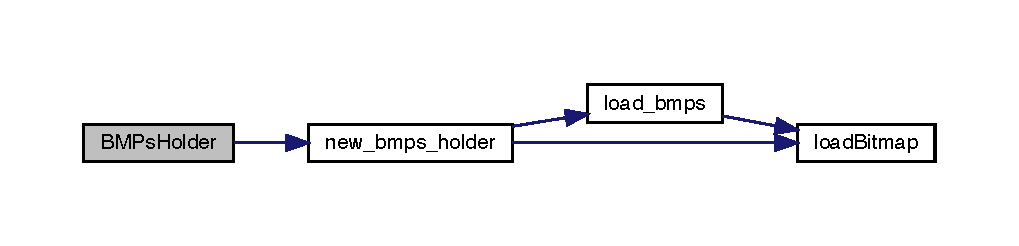
\includegraphics[width=350pt]{group___b_m_ps_holder_gafd662085ea52a83586cddd30b6423c01_cgraph}
\end{center}
\end{figure}
\hypertarget{group___b_m_ps_holder_ga72dfdb9916627f68651174c037680533}{}\label{group___b_m_ps_holder_ga72dfdb9916627f68651174c037680533} 
\index{B\+M\+Ps\+Holder@{B\+M\+Ps\+Holder}!delete\+\_\+bmps@{delete\+\_\+bmps}}
\index{delete\+\_\+bmps@{delete\+\_\+bmps}!B\+M\+Ps\+Holder@{B\+M\+Ps\+Holder}}
\subsubsection{\texorpdfstring{delete\+\_\+bmps()}{delete\_bmps()}}
{\footnotesize\ttfamily void delete\+\_\+bmps (\begin{DoxyParamCaption}\item[{\hyperlink{struct_bitmap}{Bitmap} $\ast$$\ast$}]{arr,  }\item[{unsigned}]{num }\end{DoxyParamCaption})}

Here is the call graph for this function\+:\nopagebreak
\begin{figure}[H]
\begin{center}
\leavevmode
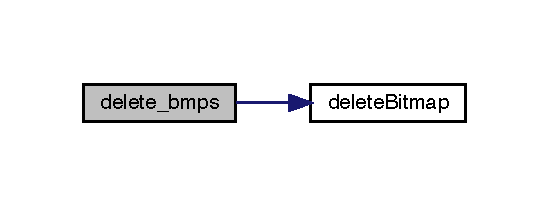
\includegraphics[width=264pt]{group___b_m_ps_holder_ga72dfdb9916627f68651174c037680533_cgraph}
\end{center}
\end{figure}
\hypertarget{group___b_m_ps_holder_gaa0a362e75eb034aa78e675ecb1b9c6da}{}\label{group___b_m_ps_holder_gaa0a362e75eb034aa78e675ecb1b9c6da} 
\index{B\+M\+Ps\+Holder@{B\+M\+Ps\+Holder}!delete\+\_\+bmps\+\_\+holder@{delete\+\_\+bmps\+\_\+holder}}
\index{delete\+\_\+bmps\+\_\+holder@{delete\+\_\+bmps\+\_\+holder}!B\+M\+Ps\+Holder@{B\+M\+Ps\+Holder}}
\subsubsection{\texorpdfstring{delete\+\_\+bmps\+\_\+holder()}{delete\_bmps\_holder()}}
{\footnotesize\ttfamily void delete\+\_\+bmps\+\_\+holder (\begin{DoxyParamCaption}{ }\end{DoxyParamCaption})}

Here is the call graph for this function\+:\nopagebreak
\begin{figure}[H]
\begin{center}
\leavevmode
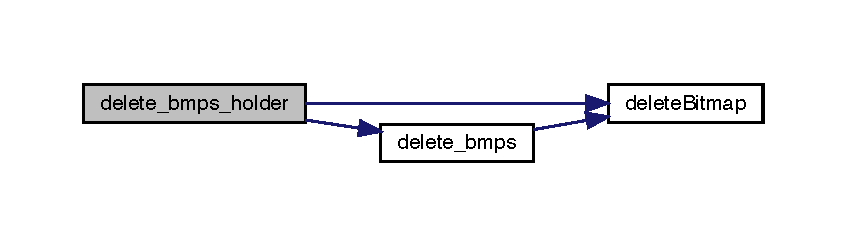
\includegraphics[width=350pt]{group___b_m_ps_holder_gaa0a362e75eb034aa78e675ecb1b9c6da_cgraph}
\end{center}
\end{figure}
\hypertarget{group___b_m_ps_holder_gab74a07b3201edddc82762946608675a5}{}\label{group___b_m_ps_holder_gab74a07b3201edddc82762946608675a5} 
\index{B\+M\+Ps\+Holder@{B\+M\+Ps\+Holder}!load\+\_\+bmps@{load\+\_\+bmps}}
\index{load\+\_\+bmps@{load\+\_\+bmps}!B\+M\+Ps\+Holder@{B\+M\+Ps\+Holder}}
\subsubsection{\texorpdfstring{load\+\_\+bmps()}{load\_bmps()}}
{\footnotesize\ttfamily \hyperlink{struct_bitmap}{Bitmap}$\ast$$\ast$ load\+\_\+bmps (\begin{DoxyParamCaption}\item[{const char $\ast$}]{base,  }\item[{unsigned}]{num }\end{DoxyParamCaption})}

Here is the call graph for this function\+:\nopagebreak
\begin{figure}[H]
\begin{center}
\leavevmode
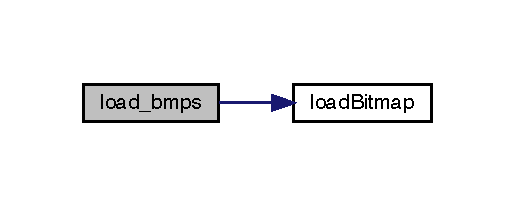
\includegraphics[width=247pt]{group___b_m_ps_holder_gab74a07b3201edddc82762946608675a5_cgraph}
\end{center}
\end{figure}

\hypertarget{group___input}{}\section{Input}
\label{group___input}\index{Input@{Input}}
\subsection*{Classes}
\begin{DoxyCompactItemize}
\item 
struct \hyperlink{struct_input__t}{Input\+\_\+t}
\begin{DoxyCompactList}\small\item\em Structure that keeps record of all the user input information. \end{DoxyCompactList}\end{DoxyCompactItemize}
\subsection*{Macros}
\begin{DoxyCompactItemize}
\item 
\#define \hyperlink{group___input_ga1d7797eb18d53b8e2b78e4255bee6050}{M\+P\+\_\+\+W\+A\+I\+T\+I\+NG}~0x01
\item 
\#define \hyperlink{group___input_ga67d21ae11c5f3ce5f1445b40f7455731}{M\+P\+\_\+\+S\+T\+A\+R\+T\+ED}~0x02
\item 
\#define \hyperlink{group___input_gabf5d93e2b77034df4441eb3e448bfb95}{M\+P\+\_\+\+E\+N\+D\+ED}~0x03
\item 
\#define \hyperlink{group___input_ga6f6489887e08bff4887d0bc5dcf214d8}{A\+CK}~0x\+FF
\end{DoxyCompactItemize}
\subsection*{Enumerations}
\begin{DoxyCompactItemize}
\item 
enum \hyperlink{group___input_gad2eda33b1d20e895223c0ebbb339bde8}{serial\+\_\+state\+\_\+t} \{ \hyperlink{group___input_ggad2eda33b1d20e895223c0ebbb339bde8acbf7d4decafc5be07eb03140ae4569ad}{W\+A\+I\+T\+I\+N\+G\+\_\+\+S\+T\+A\+RT}, 
\hyperlink{group___input_ggad2eda33b1d20e895223c0ebbb339bde8aea9e2a8ce4339ceb6af69f47c7610012}{O\+N\+G\+O\+I\+NG}, 
\hyperlink{group___input_ggad2eda33b1d20e895223c0ebbb339bde8ae793e9244aaa6de6060e251d5e0d2021}{E\+N\+D\+ED}, 
\hyperlink{group___input_ggad2eda33b1d20e895223c0ebbb339bde8ac157bdf0b85a40d2619cbc8bc1ae5fe2}{N\+O\+NE}
 \}
\item 
enum \hyperlink{group___input_ga6e68664bf6d0e0a4dac76a07ae630c52}{keycode\+\_\+t} \{ \newline
\hyperlink{group___input_gga6e68664bf6d0e0a4dac76a07ae630c52a8366c23d0d25dbbfc1bb69112a1f95a8}{E\+S\+C\+\_\+\+B\+R\+E\+AK} = E\+S\+C\+\_\+\+B\+R\+E\+A\+K\+\_\+\+C\+O\+DE, 
\hyperlink{group___input_gga6e68664bf6d0e0a4dac76a07ae630c52a01de7fd0ebd3f43151d9601a28425e24}{E\+N\+T\+E\+R\+\_\+\+B\+R\+E\+AK} = E\+N\+T\+E\+R\+\_\+\+B\+R\+E\+A\+K\+\_\+\+C\+O\+DE, 
\hyperlink{group___input_gga6e68664bf6d0e0a4dac76a07ae630c52ab53bdb8ad76cc94ac22158c433d55c4b}{U\+P\+\_\+\+M\+A\+KE} = U\+P\+\_\+\+M\+A\+K\+E\+\_\+\+C\+O\+DE, 
\hyperlink{group___input_gga6e68664bf6d0e0a4dac76a07ae630c52a56933f61ec12c9ff7723f2ef936d6c97}{D\+O\+W\+N\+\_\+\+M\+A\+KE} = D\+O\+W\+N\+\_\+\+M\+A\+K\+E\+\_\+\+C\+O\+DE, 
\newline
\hyperlink{group___input_gga6e68664bf6d0e0a4dac76a07ae630c52aec8a3617311ffdac328944fe1e482708}{N\+O\+\_\+\+K\+EY} = 0x0
 \}
\end{DoxyCompactItemize}
\subsection*{Functions}
\begin{DoxyCompactItemize}
\item 
void \hyperlink{group___input_gad26ccb83dbd3f35a93e991343682b843}{serial\+\_\+handler} ()
\begin{DoxyCompactList}\small\item\em Serial Port interrupt handler. \end{DoxyCompactList}\item 
void \hyperlink{group___input_gaaf4cb27460e9e5bfa6f46343518e89bf}{set\+Com\+State} (\hyperlink{group___input_gad2eda33b1d20e895223c0ebbb339bde8}{serial\+\_\+state\+\_\+t} state)
\begin{DoxyCompactList}\small\item\em Sets the Communication State. Used for multiplayer state. \end{DoxyCompactList}\item 
\hyperlink{group___input_gad2eda33b1d20e895223c0ebbb339bde8}{serial\+\_\+state\+\_\+t} \hyperlink{group___input_gadf520a08e359e983d9cfb73a8b714fc2}{get\+Com\+State} ()
\begin{DoxyCompactList}\small\item\em Get method for the current Communication State. \end{DoxyCompactList}\item 
\hyperlink{struct_input__t}{Input\+\_\+t} $\ast$ \hyperlink{group___input_ga8221771f8f04f39255e0b9f577c080e9}{input\+\_\+instance} ()
\begin{DoxyCompactList}\small\item\em Creates a new input instance if there is none, otherwise returns the existing one (Singleton like behaviour). \end{DoxyCompactList}\item 
void \hyperlink{group___input_ga35566b6193e5c1d1a515b309900efe82}{delete\+\_\+input} ()
\begin{DoxyCompactList}\small\item\em Destroy the Input instance, freeing all the resources used by it. \end{DoxyCompactList}\item 
void \hyperlink{group___input_ga2f4098fc71cbd39422c1001d66970bf5}{keyboard\+\_\+handler} ()
\begin{DoxyCompactList}\small\item\em Keyboard Interrupt Handler. \end{DoxyCompactList}\item 
\hyperlink{group___input_ga6e68664bf6d0e0a4dac76a07ae630c52}{keycode\+\_\+t} \hyperlink{group___input_ga4abaa84a7ae0505c6acab391f82ab1ac}{input\+\_\+get\+\_\+key} ()
\begin{DoxyCompactList}\small\item\em Remove\textquotesingle{}s the key code from the input buffer. \end{DoxyCompactList}\item 
const int $\ast$ \hyperlink{group___input_ga6ee316c978397c6807556fb9298ce902}{get\+\_\+mouse\+\_\+pos} ()
\begin{DoxyCompactList}\small\item\em Gets the current mouse position on the screen. \end{DoxyCompactList}\item 
int \hyperlink{group___input_ga5d6fc0beedad492333795ddff18c20b9}{get\+\_\+mouse\+R\+MB} ()
\begin{DoxyCompactList}\small\item\em Gets the current state of the mouse right button. \end{DoxyCompactList}\item 
int \hyperlink{group___input_gafff0cd01210126d49120f40045cafccc}{get\+\_\+mouse\+L\+MB} ()
\begin{DoxyCompactList}\small\item\em Gets the current state of the mouse left button. \end{DoxyCompactList}\item 
int \hyperlink{group___input_ga38c8f84d3704d46011eee4fd423abaa2}{get\+\_\+mouse\+M\+MB} ()
\begin{DoxyCompactList}\small\item\em Gets the current state of the mouse middle button. \end{DoxyCompactList}\item 
void \hyperlink{group___input_gaeeb5745202c4e6c62abee86ad62f36f6}{mouse\+\_\+packet\+\_\+handler} (unsigned char $\ast$packet)
\begin{DoxyCompactList}\small\item\em Mouse Interrupt Handler. \end{DoxyCompactList}\item 
int \hyperlink{group___input_gaa1aaa6e96c3e2c48378faaace6138b99}{mouse\+\_\+inside\+\_\+rect} (int x\+\_\+initial, int y\+\_\+initial, int x\+\_\+final, int y\+\_\+final)
\begin{DoxyCompactList}\small\item\em Verifies if the Mouse is inside a certain rectangle. \end{DoxyCompactList}\item 
int \hyperlink{group___input_ga287741f65ec2e6257111210ed16d3d05}{mouse\+\_\+inside\+\_\+circle} (int x\+\_\+center, int y\+\_\+center, int radius)
\begin{DoxyCompactList}\small\item\em Verifies if the Mouse is inside a certain circle. \end{DoxyCompactList}\end{DoxyCompactItemize}


\subsection{Detailed Description}
Functions for manipulating all the Inputs from the user/ player 

\subsection{Macro Definition Documentation}
\hypertarget{group___input_ga6f6489887e08bff4887d0bc5dcf214d8}{}\label{group___input_ga6f6489887e08bff4887d0bc5dcf214d8} 
\index{Input@{Input}!A\+CK@{A\+CK}}
\index{A\+CK@{A\+CK}!Input@{Input}}
\subsubsection{\texorpdfstring{A\+CK}{ACK}}
{\footnotesize\ttfamily \#define A\+CK~0x\+FF}

\hypertarget{group___input_gabf5d93e2b77034df4441eb3e448bfb95}{}\label{group___input_gabf5d93e2b77034df4441eb3e448bfb95} 
\index{Input@{Input}!M\+P\+\_\+\+E\+N\+D\+ED@{M\+P\+\_\+\+E\+N\+D\+ED}}
\index{M\+P\+\_\+\+E\+N\+D\+ED@{M\+P\+\_\+\+E\+N\+D\+ED}!Input@{Input}}
\subsubsection{\texorpdfstring{M\+P\+\_\+\+E\+N\+D\+ED}{MP\_ENDED}}
{\footnotesize\ttfamily \#define M\+P\+\_\+\+E\+N\+D\+ED~0x03}

\hypertarget{group___input_ga67d21ae11c5f3ce5f1445b40f7455731}{}\label{group___input_ga67d21ae11c5f3ce5f1445b40f7455731} 
\index{Input@{Input}!M\+P\+\_\+\+S\+T\+A\+R\+T\+ED@{M\+P\+\_\+\+S\+T\+A\+R\+T\+ED}}
\index{M\+P\+\_\+\+S\+T\+A\+R\+T\+ED@{M\+P\+\_\+\+S\+T\+A\+R\+T\+ED}!Input@{Input}}
\subsubsection{\texorpdfstring{M\+P\+\_\+\+S\+T\+A\+R\+T\+ED}{MP\_STARTED}}
{\footnotesize\ttfamily \#define M\+P\+\_\+\+S\+T\+A\+R\+T\+ED~0x02}

\hypertarget{group___input_ga1d7797eb18d53b8e2b78e4255bee6050}{}\label{group___input_ga1d7797eb18d53b8e2b78e4255bee6050} 
\index{Input@{Input}!M\+P\+\_\+\+W\+A\+I\+T\+I\+NG@{M\+P\+\_\+\+W\+A\+I\+T\+I\+NG}}
\index{M\+P\+\_\+\+W\+A\+I\+T\+I\+NG@{M\+P\+\_\+\+W\+A\+I\+T\+I\+NG}!Input@{Input}}
\subsubsection{\texorpdfstring{M\+P\+\_\+\+W\+A\+I\+T\+I\+NG}{MP\_WAITING}}
{\footnotesize\ttfamily \#define M\+P\+\_\+\+W\+A\+I\+T\+I\+NG~0x01}



\subsection{Enumeration Type Documentation}
\hypertarget{group___input_ga6e68664bf6d0e0a4dac76a07ae630c52}{}\label{group___input_ga6e68664bf6d0e0a4dac76a07ae630c52} 
\index{Input@{Input}!keycode\+\_\+t@{keycode\+\_\+t}}
\index{keycode\+\_\+t@{keycode\+\_\+t}!Input@{Input}}
\subsubsection{\texorpdfstring{keycode\+\_\+t}{keycode\_t}}
{\footnotesize\ttfamily enum \hyperlink{group___input_ga6e68664bf6d0e0a4dac76a07ae630c52}{keycode\+\_\+t}}

Keyboard scan codes that should be recognized \begin{DoxyEnumFields}{Enumerator}
\raisebox{\heightof{T}}[0pt][0pt]{\index{E\+S\+C\+\_\+\+B\+R\+E\+AK@{E\+S\+C\+\_\+\+B\+R\+E\+AK}!Input@{Input}}\index{Input@{Input}!E\+S\+C\+\_\+\+B\+R\+E\+AK@{E\+S\+C\+\_\+\+B\+R\+E\+AK}}}\hypertarget{group___input_gga6e68664bf6d0e0a4dac76a07ae630c52a8366c23d0d25dbbfc1bb69112a1f95a8}{}\label{group___input_gga6e68664bf6d0e0a4dac76a07ae630c52a8366c23d0d25dbbfc1bb69112a1f95a8} 
E\+S\+C\+\_\+\+B\+R\+E\+AK&\\
\hline

\raisebox{\heightof{T}}[0pt][0pt]{\index{E\+N\+T\+E\+R\+\_\+\+B\+R\+E\+AK@{E\+N\+T\+E\+R\+\_\+\+B\+R\+E\+AK}!Input@{Input}}\index{Input@{Input}!E\+N\+T\+E\+R\+\_\+\+B\+R\+E\+AK@{E\+N\+T\+E\+R\+\_\+\+B\+R\+E\+AK}}}\hypertarget{group___input_gga6e68664bf6d0e0a4dac76a07ae630c52a01de7fd0ebd3f43151d9601a28425e24}{}\label{group___input_gga6e68664bf6d0e0a4dac76a07ae630c52a01de7fd0ebd3f43151d9601a28425e24} 
E\+N\+T\+E\+R\+\_\+\+B\+R\+E\+AK&\\
\hline

\raisebox{\heightof{T}}[0pt][0pt]{\index{U\+P\+\_\+\+M\+A\+KE@{U\+P\+\_\+\+M\+A\+KE}!Input@{Input}}\index{Input@{Input}!U\+P\+\_\+\+M\+A\+KE@{U\+P\+\_\+\+M\+A\+KE}}}\hypertarget{group___input_gga6e68664bf6d0e0a4dac76a07ae630c52ab53bdb8ad76cc94ac22158c433d55c4b}{}\label{group___input_gga6e68664bf6d0e0a4dac76a07ae630c52ab53bdb8ad76cc94ac22158c433d55c4b} 
U\+P\+\_\+\+M\+A\+KE&\\
\hline

\raisebox{\heightof{T}}[0pt][0pt]{\index{D\+O\+W\+N\+\_\+\+M\+A\+KE@{D\+O\+W\+N\+\_\+\+M\+A\+KE}!Input@{Input}}\index{Input@{Input}!D\+O\+W\+N\+\_\+\+M\+A\+KE@{D\+O\+W\+N\+\_\+\+M\+A\+KE}}}\hypertarget{group___input_gga6e68664bf6d0e0a4dac76a07ae630c52a56933f61ec12c9ff7723f2ef936d6c97}{}\label{group___input_gga6e68664bf6d0e0a4dac76a07ae630c52a56933f61ec12c9ff7723f2ef936d6c97} 
D\+O\+W\+N\+\_\+\+M\+A\+KE&\\
\hline

\raisebox{\heightof{T}}[0pt][0pt]{\index{N\+O\+\_\+\+K\+EY@{N\+O\+\_\+\+K\+EY}!Input@{Input}}\index{Input@{Input}!N\+O\+\_\+\+K\+EY@{N\+O\+\_\+\+K\+EY}}}\hypertarget{group___input_gga6e68664bf6d0e0a4dac76a07ae630c52aec8a3617311ffdac328944fe1e482708}{}\label{group___input_gga6e68664bf6d0e0a4dac76a07ae630c52aec8a3617311ffdac328944fe1e482708} 
N\+O\+\_\+\+K\+EY&\\
\hline

\end{DoxyEnumFields}
\hypertarget{group___input_gad2eda33b1d20e895223c0ebbb339bde8}{}\label{group___input_gad2eda33b1d20e895223c0ebbb339bde8} 
\index{Input@{Input}!serial\+\_\+state\+\_\+t@{serial\+\_\+state\+\_\+t}}
\index{serial\+\_\+state\+\_\+t@{serial\+\_\+state\+\_\+t}!Input@{Input}}
\subsubsection{\texorpdfstring{serial\+\_\+state\+\_\+t}{serial\_state\_t}}
{\footnotesize\ttfamily enum \hyperlink{group___input_gad2eda33b1d20e895223c0ebbb339bde8}{serial\+\_\+state\+\_\+t}}

\begin{DoxyEnumFields}{Enumerator}
\raisebox{\heightof{T}}[0pt][0pt]{\index{W\+A\+I\+T\+I\+N\+G\+\_\+\+S\+T\+A\+RT@{W\+A\+I\+T\+I\+N\+G\+\_\+\+S\+T\+A\+RT}!Input@{Input}}\index{Input@{Input}!W\+A\+I\+T\+I\+N\+G\+\_\+\+S\+T\+A\+RT@{W\+A\+I\+T\+I\+N\+G\+\_\+\+S\+T\+A\+RT}}}\hypertarget{group___input_ggad2eda33b1d20e895223c0ebbb339bde8acbf7d4decafc5be07eb03140ae4569ad}{}\label{group___input_ggad2eda33b1d20e895223c0ebbb339bde8acbf7d4decafc5be07eb03140ae4569ad} 
W\+A\+I\+T\+I\+N\+G\+\_\+\+S\+T\+A\+RT&\\
\hline

\raisebox{\heightof{T}}[0pt][0pt]{\index{O\+N\+G\+O\+I\+NG@{O\+N\+G\+O\+I\+NG}!Input@{Input}}\index{Input@{Input}!O\+N\+G\+O\+I\+NG@{O\+N\+G\+O\+I\+NG}}}\hypertarget{group___input_ggad2eda33b1d20e895223c0ebbb339bde8aea9e2a8ce4339ceb6af69f47c7610012}{}\label{group___input_ggad2eda33b1d20e895223c0ebbb339bde8aea9e2a8ce4339ceb6af69f47c7610012} 
O\+N\+G\+O\+I\+NG&\\
\hline

\raisebox{\heightof{T}}[0pt][0pt]{\index{E\+N\+D\+ED@{E\+N\+D\+ED}!Input@{Input}}\index{Input@{Input}!E\+N\+D\+ED@{E\+N\+D\+ED}}}\hypertarget{group___input_ggad2eda33b1d20e895223c0ebbb339bde8ae793e9244aaa6de6060e251d5e0d2021}{}\label{group___input_ggad2eda33b1d20e895223c0ebbb339bde8ae793e9244aaa6de6060e251d5e0d2021} 
E\+N\+D\+ED&\\
\hline

\raisebox{\heightof{T}}[0pt][0pt]{\index{N\+O\+NE@{N\+O\+NE}!Input@{Input}}\index{Input@{Input}!N\+O\+NE@{N\+O\+NE}}}\hypertarget{group___input_ggad2eda33b1d20e895223c0ebbb339bde8ac157bdf0b85a40d2619cbc8bc1ae5fe2}{}\label{group___input_ggad2eda33b1d20e895223c0ebbb339bde8ac157bdf0b85a40d2619cbc8bc1ae5fe2} 
N\+O\+NE&\\
\hline

\end{DoxyEnumFields}


\subsection{Function Documentation}
\hypertarget{group___input_ga35566b6193e5c1d1a515b309900efe82}{}\label{group___input_ga35566b6193e5c1d1a515b309900efe82} 
\index{Input@{Input}!delete\+\_\+input@{delete\+\_\+input}}
\index{delete\+\_\+input@{delete\+\_\+input}!Input@{Input}}
\subsubsection{\texorpdfstring{delete\+\_\+input()}{delete\_input()}}
{\footnotesize\ttfamily void delete\+\_\+input (\begin{DoxyParamCaption}{ }\end{DoxyParamCaption})}



Destroy the Input instance, freeing all the resources used by it. 

Here is the call graph for this function\+:\nopagebreak
\begin{figure}[H]
\begin{center}
\leavevmode
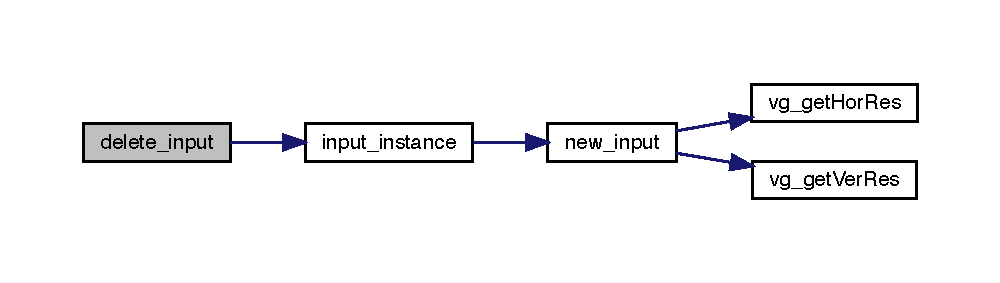
\includegraphics[width=350pt]{group___input_ga35566b6193e5c1d1a515b309900efe82_cgraph}
\end{center}
\end{figure}
\hypertarget{group___input_ga6ee316c978397c6807556fb9298ce902}{}\label{group___input_ga6ee316c978397c6807556fb9298ce902} 
\index{Input@{Input}!get\+\_\+mouse\+\_\+pos@{get\+\_\+mouse\+\_\+pos}}
\index{get\+\_\+mouse\+\_\+pos@{get\+\_\+mouse\+\_\+pos}!Input@{Input}}
\subsubsection{\texorpdfstring{get\+\_\+mouse\+\_\+pos()}{get\_mouse\_pos()}}
{\footnotesize\ttfamily const int$\ast$ get\+\_\+mouse\+\_\+pos (\begin{DoxyParamCaption}{ }\end{DoxyParamCaption})}



Gets the current mouse position on the screen. 

\begin{DoxyReturn}{Returns}
Array containing the current mouse position on the screen (x,y) 
\end{DoxyReturn}
Here is the call graph for this function\+:\nopagebreak
\begin{figure}[H]
\begin{center}
\leavevmode
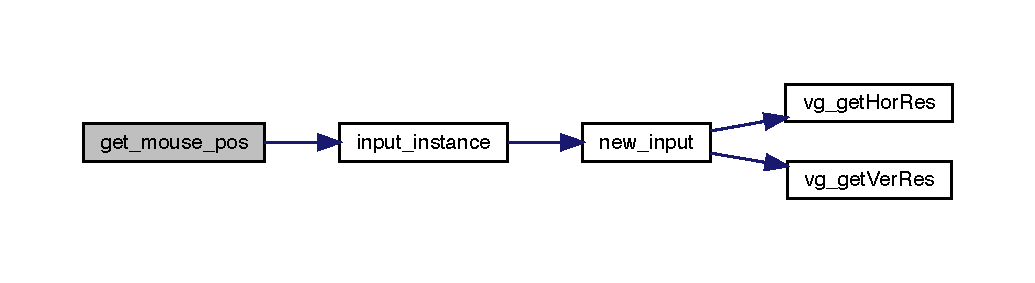
\includegraphics[width=350pt]{group___input_ga6ee316c978397c6807556fb9298ce902_cgraph}
\end{center}
\end{figure}
\hypertarget{group___input_gafff0cd01210126d49120f40045cafccc}{}\label{group___input_gafff0cd01210126d49120f40045cafccc} 
\index{Input@{Input}!get\+\_\+mouse\+L\+MB@{get\+\_\+mouse\+L\+MB}}
\index{get\+\_\+mouse\+L\+MB@{get\+\_\+mouse\+L\+MB}!Input@{Input}}
\subsubsection{\texorpdfstring{get\+\_\+mouse\+L\+M\+B()}{get\_mouseLMB()}}
{\footnotesize\ttfamily int get\+\_\+mouse\+L\+MB (\begin{DoxyParamCaption}{ }\end{DoxyParamCaption})}



Gets the current state of the mouse left button. 

\begin{DoxyReturn}{Returns}
Return 0 if mouse left button is not pressed, non zero otherwise 
\end{DoxyReturn}
Here is the call graph for this function\+:\nopagebreak
\begin{figure}[H]
\begin{center}
\leavevmode
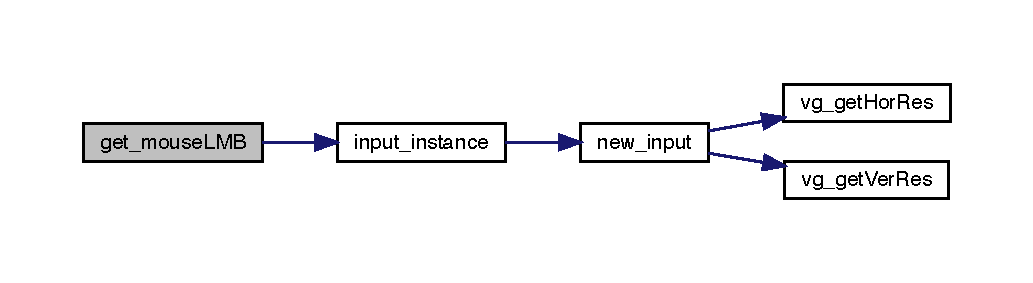
\includegraphics[width=350pt]{group___input_gafff0cd01210126d49120f40045cafccc_cgraph}
\end{center}
\end{figure}
\hypertarget{group___input_ga38c8f84d3704d46011eee4fd423abaa2}{}\label{group___input_ga38c8f84d3704d46011eee4fd423abaa2} 
\index{Input@{Input}!get\+\_\+mouse\+M\+MB@{get\+\_\+mouse\+M\+MB}}
\index{get\+\_\+mouse\+M\+MB@{get\+\_\+mouse\+M\+MB}!Input@{Input}}
\subsubsection{\texorpdfstring{get\+\_\+mouse\+M\+M\+B()}{get\_mouseMMB()}}
{\footnotesize\ttfamily int get\+\_\+mouse\+M\+MB (\begin{DoxyParamCaption}{ }\end{DoxyParamCaption})}



Gets the current state of the mouse middle button. 

\begin{DoxyReturn}{Returns}
Return 0 if mouse middle button is not pressed, non zero otherwise 
\end{DoxyReturn}
Here is the call graph for this function\+:\nopagebreak
\begin{figure}[H]
\begin{center}
\leavevmode
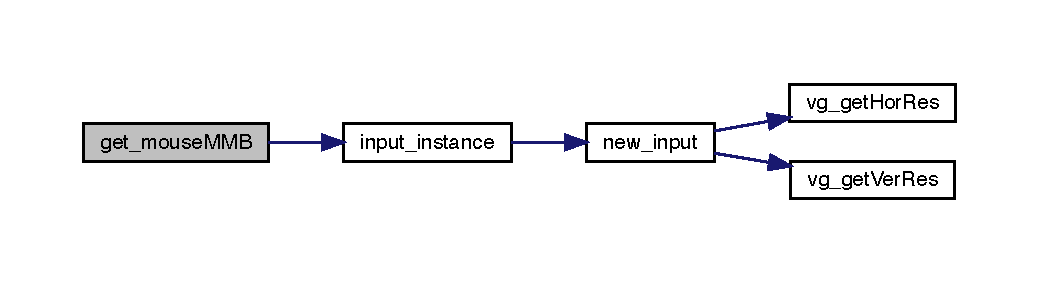
\includegraphics[width=350pt]{group___input_ga38c8f84d3704d46011eee4fd423abaa2_cgraph}
\end{center}
\end{figure}
\hypertarget{group___input_ga5d6fc0beedad492333795ddff18c20b9}{}\label{group___input_ga5d6fc0beedad492333795ddff18c20b9} 
\index{Input@{Input}!get\+\_\+mouse\+R\+MB@{get\+\_\+mouse\+R\+MB}}
\index{get\+\_\+mouse\+R\+MB@{get\+\_\+mouse\+R\+MB}!Input@{Input}}
\subsubsection{\texorpdfstring{get\+\_\+mouse\+R\+M\+B()}{get\_mouseRMB()}}
{\footnotesize\ttfamily int get\+\_\+mouse\+R\+MB (\begin{DoxyParamCaption}{ }\end{DoxyParamCaption})}



Gets the current state of the mouse right button. 

\begin{DoxyReturn}{Returns}
Return 0 if mouse right button is not pressed, non zero otherwise 
\end{DoxyReturn}
Here is the call graph for this function\+:\nopagebreak
\begin{figure}[H]
\begin{center}
\leavevmode
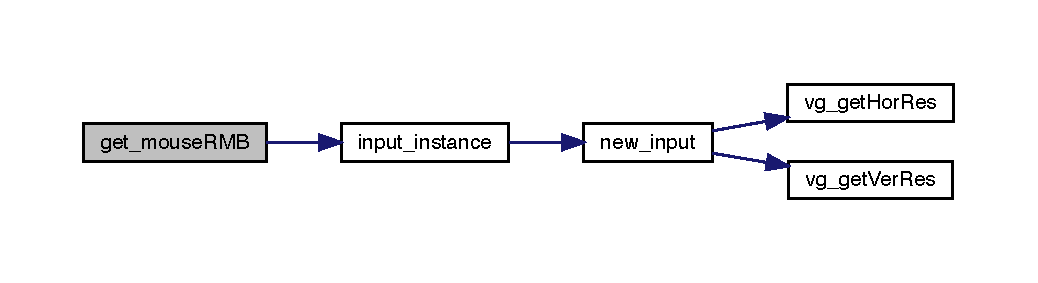
\includegraphics[width=350pt]{group___input_ga5d6fc0beedad492333795ddff18c20b9_cgraph}
\end{center}
\end{figure}
\hypertarget{group___input_gadf520a08e359e983d9cfb73a8b714fc2}{}\label{group___input_gadf520a08e359e983d9cfb73a8b714fc2} 
\index{Input@{Input}!get\+Com\+State@{get\+Com\+State}}
\index{get\+Com\+State@{get\+Com\+State}!Input@{Input}}
\subsubsection{\texorpdfstring{get\+Com\+State()}{getComState()}}
{\footnotesize\ttfamily \hyperlink{group___input_gad2eda33b1d20e895223c0ebbb339bde8}{serial\+\_\+state\+\_\+t} get\+Com\+State (\begin{DoxyParamCaption}{ }\end{DoxyParamCaption})}



Get method for the current Communication State. 

\begin{DoxyReturn}{Returns}
The current serial\+\_\+state\+\_\+t 
\end{DoxyReturn}
\hypertarget{group___input_ga4abaa84a7ae0505c6acab391f82ab1ac}{}\label{group___input_ga4abaa84a7ae0505c6acab391f82ab1ac} 
\index{Input@{Input}!input\+\_\+get\+\_\+key@{input\+\_\+get\+\_\+key}}
\index{input\+\_\+get\+\_\+key@{input\+\_\+get\+\_\+key}!Input@{Input}}
\subsubsection{\texorpdfstring{input\+\_\+get\+\_\+key()}{input\_get\_key()}}
{\footnotesize\ttfamily \hyperlink{group___input_ga6e68664bf6d0e0a4dac76a07ae630c52}{keycode\+\_\+t} input\+\_\+get\+\_\+key (\begin{DoxyParamCaption}{ }\end{DoxyParamCaption})}



Remove\textquotesingle{}s the key code from the input buffer. 

Compatible with double make/ brake codes

\begin{DoxyReturn}{Returns}
Key code type (E\+SC, E\+N\+T\+ER, UP, D\+O\+WN or N\+O\+NE) 
\end{DoxyReturn}
Here is the call graph for this function\+:
\nopagebreak
\begin{figure}[H]
\begin{center}
\leavevmode
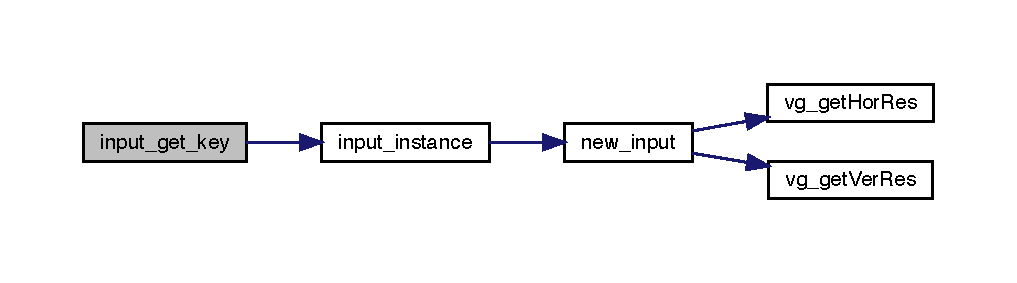
\includegraphics[width=350pt]{group___input_ga4abaa84a7ae0505c6acab391f82ab1ac_cgraph}
\end{center}
\end{figure}
\hypertarget{group___input_ga8221771f8f04f39255e0b9f577c080e9}{}\label{group___input_ga8221771f8f04f39255e0b9f577c080e9} 
\index{Input@{Input}!input\+\_\+instance@{input\+\_\+instance}}
\index{input\+\_\+instance@{input\+\_\+instance}!Input@{Input}}
\subsubsection{\texorpdfstring{input\+\_\+instance()}{input\_instance()}}
{\footnotesize\ttfamily \hyperlink{struct_input__t}{Input\+\_\+t}$\ast$ input\+\_\+instance (\begin{DoxyParamCaption}{ }\end{DoxyParamCaption})}



Creates a new input instance if there is none, otherwise returns the existing one (Singleton like behaviour). 

\begin{DoxyReturn}{Returns}
Pointer to a Input instance 
\end{DoxyReturn}
Here is the call graph for this function\+:
\nopagebreak
\begin{figure}[H]
\begin{center}
\leavevmode
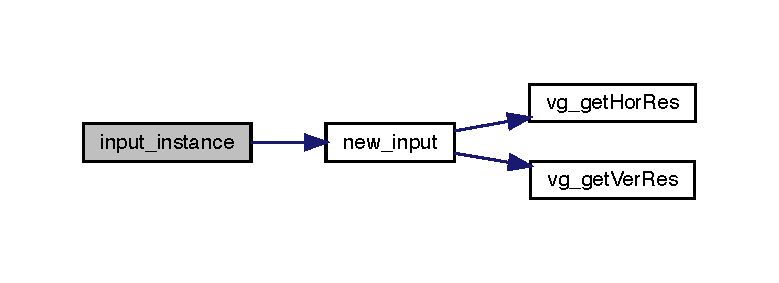
\includegraphics[width=350pt]{group___input_ga8221771f8f04f39255e0b9f577c080e9_cgraph}
\end{center}
\end{figure}
\hypertarget{group___input_ga2f4098fc71cbd39422c1001d66970bf5}{}\label{group___input_ga2f4098fc71cbd39422c1001d66970bf5} 
\index{Input@{Input}!keyboard\+\_\+handler@{keyboard\+\_\+handler}}
\index{keyboard\+\_\+handler@{keyboard\+\_\+handler}!Input@{Input}}
\subsubsection{\texorpdfstring{keyboard\+\_\+handler()}{keyboard\_handler()}}
{\footnotesize\ttfamily void keyboard\+\_\+handler (\begin{DoxyParamCaption}{ }\end{DoxyParamCaption})}



Keyboard Interrupt Handler. 

Here is the call graph for this function\+:
\nopagebreak
\begin{figure}[H]
\begin{center}
\leavevmode
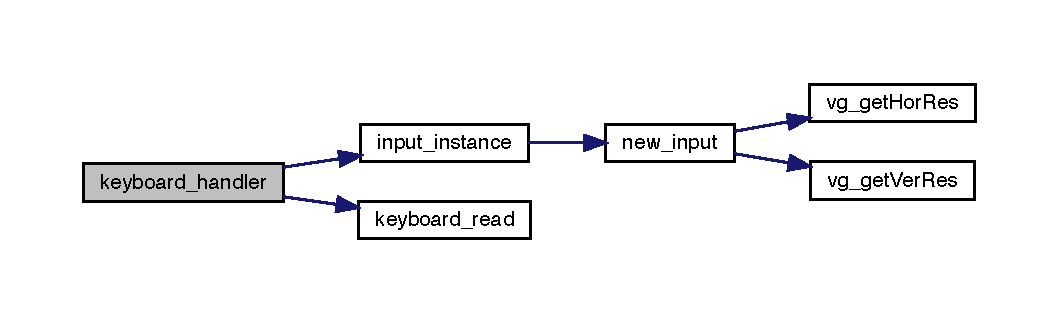
\includegraphics[width=350pt]{group___input_ga2f4098fc71cbd39422c1001d66970bf5_cgraph}
\end{center}
\end{figure}
\hypertarget{group___input_ga287741f65ec2e6257111210ed16d3d05}{}\label{group___input_ga287741f65ec2e6257111210ed16d3d05} 
\index{Input@{Input}!mouse\+\_\+inside\+\_\+circle@{mouse\+\_\+inside\+\_\+circle}}
\index{mouse\+\_\+inside\+\_\+circle@{mouse\+\_\+inside\+\_\+circle}!Input@{Input}}
\subsubsection{\texorpdfstring{mouse\+\_\+inside\+\_\+circle()}{mouse\_inside\_circle()}}
{\footnotesize\ttfamily int mouse\+\_\+inside\+\_\+circle (\begin{DoxyParamCaption}\item[{int}]{x\+\_\+center,  }\item[{int}]{y\+\_\+center,  }\item[{int}]{radius }\end{DoxyParamCaption})}



Verifies if the Mouse is inside a certain circle. 


\begin{DoxyParams}{Parameters}
{\em x\+\_\+center} & Position of the center of the circle in the horizontal axis \\
\hline
{\em y\+\_\+center} & Position of the center of the circle in the vertical axis \\
\hline
{\em radius} & Radius of the circle\\
\hline
\end{DoxyParams}
\begin{DoxyReturn}{Returns}
Return 0 if Mouse is not inside the circle, 1 otherwise 
\end{DoxyReturn}
Here is the call graph for this function\+:
\nopagebreak
\begin{figure}[H]
\begin{center}
\leavevmode
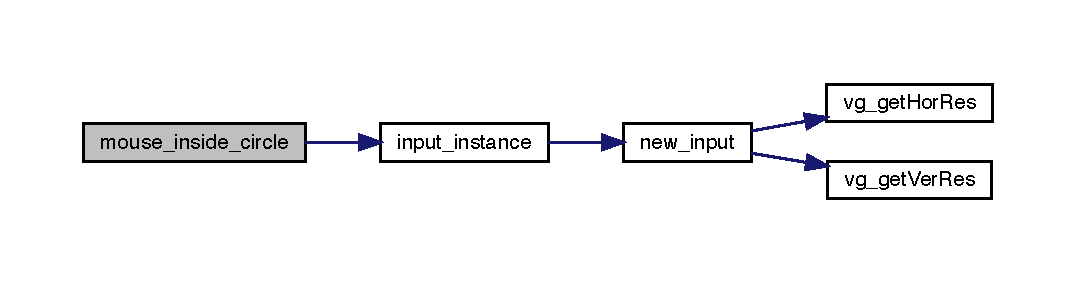
\includegraphics[width=350pt]{group___input_ga287741f65ec2e6257111210ed16d3d05_cgraph}
\end{center}
\end{figure}
\hypertarget{group___input_gaa1aaa6e96c3e2c48378faaace6138b99}{}\label{group___input_gaa1aaa6e96c3e2c48378faaace6138b99} 
\index{Input@{Input}!mouse\+\_\+inside\+\_\+rect@{mouse\+\_\+inside\+\_\+rect}}
\index{mouse\+\_\+inside\+\_\+rect@{mouse\+\_\+inside\+\_\+rect}!Input@{Input}}
\subsubsection{\texorpdfstring{mouse\+\_\+inside\+\_\+rect()}{mouse\_inside\_rect()}}
{\footnotesize\ttfamily int mouse\+\_\+inside\+\_\+rect (\begin{DoxyParamCaption}\item[{int}]{x\+\_\+initial,  }\item[{int}]{y\+\_\+initial,  }\item[{int}]{x\+\_\+final,  }\item[{int}]{y\+\_\+final }\end{DoxyParamCaption})}



Verifies if the Mouse is inside a certain rectangle. 


\begin{DoxyParams}{Parameters}
{\em x\+\_\+inital} & Initial position of the rectangle in the horizontal axis \\
\hline
{\em y\+\_\+initial} & Initial position of the rectangle in the vertical axis \\
\hline
{\em x\+\_\+final} & Final position of the rectangle in the horizontal axis \\
\hline
{\em y\+\_\+final} & Final position of the rectangle in the vertical axis\\
\hline
\end{DoxyParams}
\begin{DoxyReturn}{Returns}
Return 0 if Mouse is not inside the rectantgle, 1 otherwise 
\end{DoxyReturn}
Here is the call graph for this function\+:
\nopagebreak
\begin{figure}[H]
\begin{center}
\leavevmode
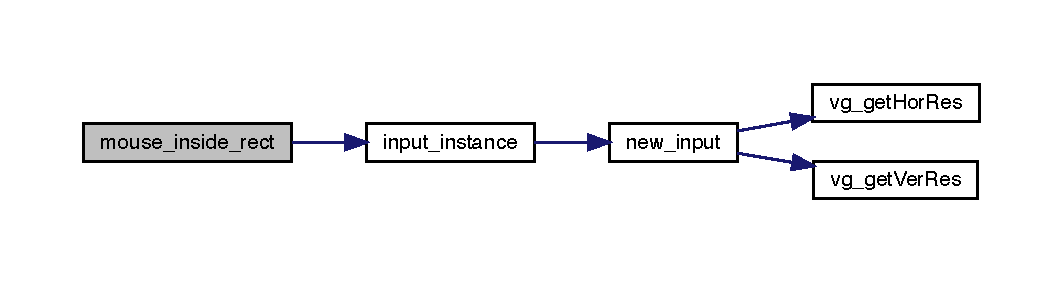
\includegraphics[width=350pt]{group___input_gaa1aaa6e96c3e2c48378faaace6138b99_cgraph}
\end{center}
\end{figure}
\hypertarget{group___input_gaeeb5745202c4e6c62abee86ad62f36f6}{}\label{group___input_gaeeb5745202c4e6c62abee86ad62f36f6} 
\index{Input@{Input}!mouse\+\_\+packet\+\_\+handler@{mouse\+\_\+packet\+\_\+handler}}
\index{mouse\+\_\+packet\+\_\+handler@{mouse\+\_\+packet\+\_\+handler}!Input@{Input}}
\subsubsection{\texorpdfstring{mouse\+\_\+packet\+\_\+handler()}{mouse\_packet\_handler()}}
{\footnotesize\ttfamily void mouse\+\_\+packet\+\_\+handler (\begin{DoxyParamCaption}\item[{unsigned char $\ast$}]{packet }\end{DoxyParamCaption})}



Mouse Interrupt Handler. 

Reads the packet received and updates the Input instance accordingly


\begin{DoxyParams}{Parameters}
{\em packet} & mouse packet containing the mouse information \\
\hline
\end{DoxyParams}
Update Buttons

Update Position Here is the call graph for this function\+:
\nopagebreak
\begin{figure}[H]
\begin{center}
\leavevmode
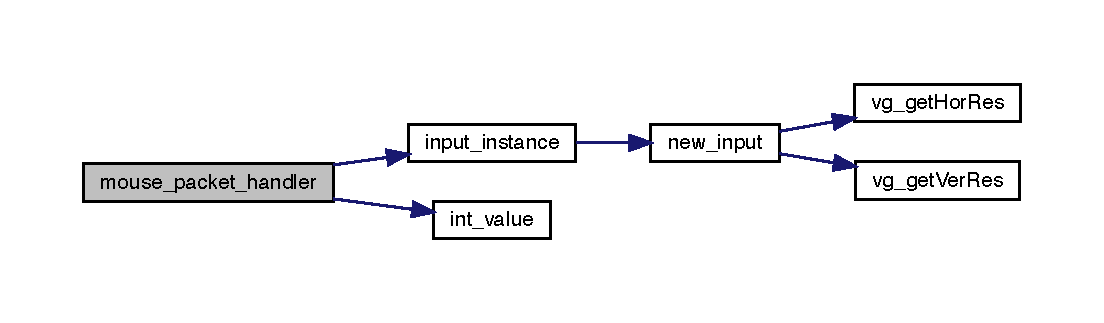
\includegraphics[width=350pt]{group___input_gaeeb5745202c4e6c62abee86ad62f36f6_cgraph}
\end{center}
\end{figure}
\hypertarget{group___input_gad26ccb83dbd3f35a93e991343682b843}{}\label{group___input_gad26ccb83dbd3f35a93e991343682b843} 
\index{Input@{Input}!serial\+\_\+handler@{serial\+\_\+handler}}
\index{serial\+\_\+handler@{serial\+\_\+handler}!Input@{Input}}
\subsubsection{\texorpdfstring{serial\+\_\+handler()}{serial\_handler()}}
{\footnotesize\ttfamily void serial\+\_\+handler (\begin{DoxyParamCaption}{ }\end{DoxyParamCaption})}



Serial Port interrupt handler. 

Here is the call graph for this function\+:
\nopagebreak
\begin{figure}[H]
\begin{center}
\leavevmode
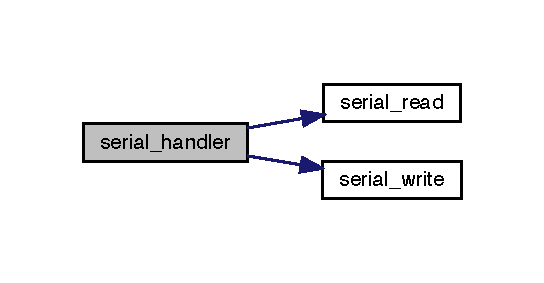
\includegraphics[width=261pt]{group___input_gad26ccb83dbd3f35a93e991343682b843_cgraph}
\end{center}
\end{figure}
\hypertarget{group___input_gaaf4cb27460e9e5bfa6f46343518e89bf}{}\label{group___input_gaaf4cb27460e9e5bfa6f46343518e89bf} 
\index{Input@{Input}!set\+Com\+State@{set\+Com\+State}}
\index{set\+Com\+State@{set\+Com\+State}!Input@{Input}}
\subsubsection{\texorpdfstring{set\+Com\+State()}{setComState()}}
{\footnotesize\ttfamily void set\+Com\+State (\begin{DoxyParamCaption}\item[{\hyperlink{group___input_gad2eda33b1d20e895223c0ebbb339bde8}{serial\+\_\+state\+\_\+t}}]{state }\end{DoxyParamCaption})}



Sets the Communication State. Used for multiplayer state. 


\hypertarget{group___g_vector}{}\section{G\+Vector}
\label{group___g_vector}\index{G\+Vector@{G\+Vector}}
\subsection*{Typedefs}
\begin{DoxyCompactItemize}
\item 
typedef struct \hyperlink{structgvector__t}{gvector\+\_\+t} \hyperlink{group___g_vector_ga6d90d5e6b721779a43354f2752b79281}{G\+Vector}
\end{DoxyCompactItemize}
\subsection*{Functions}
\begin{DoxyCompactItemize}
\item 
\hyperlink{group___g_vector_ga6d90d5e6b721779a43354f2752b79281}{G\+Vector} $\ast$ \hyperlink{group___g_vector_gae4381c0ccdbebaa240e06595e59c5712}{new\+\_\+gvector} (unsigned el\+\_\+size)
\begin{DoxyCompactList}\small\item\em Constructs a new G\+Vector. \end{DoxyCompactList}\item 
void \hyperlink{group___g_vector_gab3513aa2ddf9e3016d4be27fff810b39}{delete\+\_\+gvector} (\hyperlink{group___g_vector_ga6d90d5e6b721779a43354f2752b79281}{G\+Vector} $\ast$self)
\begin{DoxyCompactList}\small\item\em Deletes a G\+Vector, freeing all the allocated memory. \end{DoxyCompactList}\item 
unsigned \hyperlink{group___g_vector_ga3570990e6e22e8bd76cceec25869e117}{gvector\+\_\+get\+\_\+size} (\hyperlink{group___g_vector_ga6d90d5e6b721779a43354f2752b79281}{G\+Vector} $\ast$self)
\begin{DoxyCompactList}\small\item\em Gets the size (number of elements) of a G\+Vector. \end{DoxyCompactList}\item 
void $\ast$ \hyperlink{group___g_vector_ga01efe5e5a35c4656de07aa3b1c937b0b}{gvector\+\_\+at} (\hyperlink{group___g_vector_ga6d90d5e6b721779a43354f2752b79281}{G\+Vector} $\ast$self, unsigned idx)
\begin{DoxyCompactList}\small\item\em Access to an element at a given index. \end{DoxyCompactList}\item 
void $\ast$ \hyperlink{group___g_vector_ga638f666cc999e6b840302ca1de552b85}{gvector\+\_\+push\+\_\+back} (\hyperlink{group___g_vector_ga6d90d5e6b721779a43354f2752b79281}{G\+Vector} $\ast$self, void $\ast$elem)
\begin{DoxyCompactList}\small\item\em Pushes back a new element to the G\+Vector. Memory reallocation may happen. \end{DoxyCompactList}\item 
void \hyperlink{group___g_vector_ga7efdee3a454559bde23b23f31d40b4db}{gvector\+\_\+erase} (\hyperlink{group___g_vector_ga6d90d5e6b721779a43354f2752b79281}{G\+Vector} $\ast$self, unsigned idx)
\begin{DoxyCompactList}\small\item\em Erases an element at a given index. Memory reallocation may happen. \end{DoxyCompactList}\item 
void \hyperlink{group___g_vector_ga6fd765130f11b97b8fcca59d7c4e98d1}{gvector\+\_\+pop\+\_\+back} (\hyperlink{group___g_vector_ga6d90d5e6b721779a43354f2752b79281}{G\+Vector} $\ast$self)
\begin{DoxyCompactList}\small\item\em Erases the last element of G\+Vector. Memory reallocation may happen. \end{DoxyCompactList}\item 
void \hyperlink{group___g_vector_ga58f71f3cb3c10d00005e3f58951a9184}{gvector\+\_\+clear} (\hyperlink{group___g_vector_ga6d90d5e6b721779a43354f2752b79281}{G\+Vector} $\ast$self)
\begin{DoxyCompactList}\small\item\em Erases all elements of G\+Vector. Memory reallocation may happen. \end{DoxyCompactList}\end{DoxyCompactItemize}


\subsection{Detailed Description}
Functions for the usage of a G\+Vector -\/ Generic Vector 

\subsection{Typedef Documentation}
\hypertarget{group___g_vector_ga6d90d5e6b721779a43354f2752b79281}{}\label{group___g_vector_ga6d90d5e6b721779a43354f2752b79281} 
\index{G\+Vector@{G\+Vector}!G\+Vector@{G\+Vector}}
\index{G\+Vector@{G\+Vector}!G\+Vector@{G\+Vector}}
\subsubsection{\texorpdfstring{G\+Vector}{GVector}}
{\footnotesize\ttfamily typedef struct \hyperlink{structgvector__t}{gvector\+\_\+t} \hyperlink{group___g_vector_ga6d90d5e6b721779a43354f2752b79281}{G\+Vector}}



\subsection{Function Documentation}
\hypertarget{group___g_vector_gab3513aa2ddf9e3016d4be27fff810b39}{}\label{group___g_vector_gab3513aa2ddf9e3016d4be27fff810b39} 
\index{G\+Vector@{G\+Vector}!delete\+\_\+gvector@{delete\+\_\+gvector}}
\index{delete\+\_\+gvector@{delete\+\_\+gvector}!G\+Vector@{G\+Vector}}
\subsubsection{\texorpdfstring{delete\+\_\+gvector()}{delete\_gvector()}}
{\footnotesize\ttfamily void delete\+\_\+gvector (\begin{DoxyParamCaption}\item[{\hyperlink{group___g_vector_ga6d90d5e6b721779a43354f2752b79281}{G\+Vector} $\ast$}]{self }\end{DoxyParamCaption})}



Deletes a G\+Vector, freeing all the allocated memory. 


\begin{DoxyParams}{Parameters}
{\em ptr} & Pointer to the G\+Vector to be deleted \\
\hline
\end{DoxyParams}
\hypertarget{group___g_vector_ga01efe5e5a35c4656de07aa3b1c937b0b}{}\label{group___g_vector_ga01efe5e5a35c4656de07aa3b1c937b0b} 
\index{G\+Vector@{G\+Vector}!gvector\+\_\+at@{gvector\+\_\+at}}
\index{gvector\+\_\+at@{gvector\+\_\+at}!G\+Vector@{G\+Vector}}
\subsubsection{\texorpdfstring{gvector\+\_\+at()}{gvector\_at()}}
{\footnotesize\ttfamily void$\ast$ gvector\+\_\+at (\begin{DoxyParamCaption}\item[{\hyperlink{group___g_vector_ga6d90d5e6b721779a43354f2752b79281}{G\+Vector} $\ast$}]{self,  }\item[{unsigned}]{idx }\end{DoxyParamCaption})}



Access to an element at a given index. 


\begin{DoxyParams}{Parameters}
{\em self} & The G\+Vector to access \\
\hline
{\em idx} & The element\textquotesingle{}s index\\
\hline
\end{DoxyParams}
\begin{DoxyReturn}{Returns}
Pointer to the element at index idx, must be cast to the appropriate type 
\end{DoxyReturn}
\hypertarget{group___g_vector_ga58f71f3cb3c10d00005e3f58951a9184}{}\label{group___g_vector_ga58f71f3cb3c10d00005e3f58951a9184} 
\index{G\+Vector@{G\+Vector}!gvector\+\_\+clear@{gvector\+\_\+clear}}
\index{gvector\+\_\+clear@{gvector\+\_\+clear}!G\+Vector@{G\+Vector}}
\subsubsection{\texorpdfstring{gvector\+\_\+clear()}{gvector\_clear()}}
{\footnotesize\ttfamily void gvector\+\_\+clear (\begin{DoxyParamCaption}\item[{\hyperlink{group___g_vector_ga6d90d5e6b721779a43354f2752b79281}{G\+Vector} $\ast$}]{self }\end{DoxyParamCaption})}



Erases all elements of G\+Vector. Memory reallocation may happen. 


\begin{DoxyParams}{Parameters}
{\em self} & The G\+Vector to access \\
\hline
\end{DoxyParams}
Here is the call graph for this function\+:\nopagebreak
\begin{figure}[H]
\begin{center}
\leavevmode
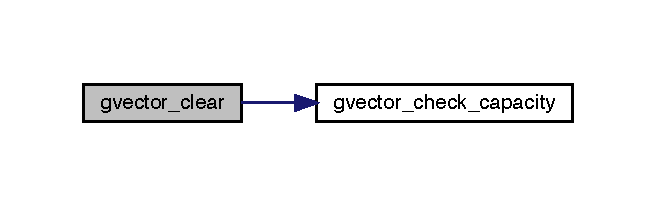
\includegraphics[width=315pt]{group___g_vector_ga58f71f3cb3c10d00005e3f58951a9184_cgraph}
\end{center}
\end{figure}
\hypertarget{group___g_vector_ga7efdee3a454559bde23b23f31d40b4db}{}\label{group___g_vector_ga7efdee3a454559bde23b23f31d40b4db} 
\index{G\+Vector@{G\+Vector}!gvector\+\_\+erase@{gvector\+\_\+erase}}
\index{gvector\+\_\+erase@{gvector\+\_\+erase}!G\+Vector@{G\+Vector}}
\subsubsection{\texorpdfstring{gvector\+\_\+erase()}{gvector\_erase()}}
{\footnotesize\ttfamily void gvector\+\_\+erase (\begin{DoxyParamCaption}\item[{\hyperlink{group___g_vector_ga6d90d5e6b721779a43354f2752b79281}{G\+Vector} $\ast$}]{self,  }\item[{unsigned}]{idx }\end{DoxyParamCaption})}



Erases an element at a given index. Memory reallocation may happen. 


\begin{DoxyParams}{Parameters}
{\em self} & The G\+Vector to access \\
\hline
{\em idx} & The index of the element to be erased \\
\hline
\end{DoxyParams}
Here is the call graph for this function\+:\nopagebreak
\begin{figure}[H]
\begin{center}
\leavevmode
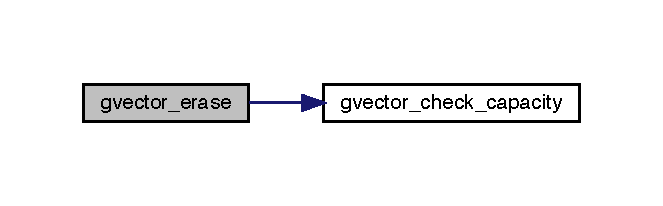
\includegraphics[width=318pt]{group___g_vector_ga7efdee3a454559bde23b23f31d40b4db_cgraph}
\end{center}
\end{figure}
\hypertarget{group___g_vector_ga3570990e6e22e8bd76cceec25869e117}{}\label{group___g_vector_ga3570990e6e22e8bd76cceec25869e117} 
\index{G\+Vector@{G\+Vector}!gvector\+\_\+get\+\_\+size@{gvector\+\_\+get\+\_\+size}}
\index{gvector\+\_\+get\+\_\+size@{gvector\+\_\+get\+\_\+size}!G\+Vector@{G\+Vector}}
\subsubsection{\texorpdfstring{gvector\+\_\+get\+\_\+size()}{gvector\_get\_size()}}
{\footnotesize\ttfamily unsigned gvector\+\_\+get\+\_\+size (\begin{DoxyParamCaption}\item[{\hyperlink{group___g_vector_ga6d90d5e6b721779a43354f2752b79281}{G\+Vector} $\ast$}]{self }\end{DoxyParamCaption})}



Gets the size (number of elements) of a G\+Vector. 


\begin{DoxyParams}{Parameters}
{\em self} & Pointer to the G\+Vector\\
\hline
\end{DoxyParams}
\begin{DoxyReturn}{Returns}
The number of elements in the G\+Vector 
\end{DoxyReturn}
\hypertarget{group___g_vector_ga6fd765130f11b97b8fcca59d7c4e98d1}{}\label{group___g_vector_ga6fd765130f11b97b8fcca59d7c4e98d1} 
\index{G\+Vector@{G\+Vector}!gvector\+\_\+pop\+\_\+back@{gvector\+\_\+pop\+\_\+back}}
\index{gvector\+\_\+pop\+\_\+back@{gvector\+\_\+pop\+\_\+back}!G\+Vector@{G\+Vector}}
\subsubsection{\texorpdfstring{gvector\+\_\+pop\+\_\+back()}{gvector\_pop\_back()}}
{\footnotesize\ttfamily void gvector\+\_\+pop\+\_\+back (\begin{DoxyParamCaption}\item[{\hyperlink{group___g_vector_ga6d90d5e6b721779a43354f2752b79281}{G\+Vector} $\ast$}]{self }\end{DoxyParamCaption})}



Erases the last element of G\+Vector. Memory reallocation may happen. 


\begin{DoxyParams}{Parameters}
{\em self} & The G\+Vector to access \\
\hline
\end{DoxyParams}
Here is the call graph for this function\+:\nopagebreak
\begin{figure}[H]
\begin{center}
\leavevmode
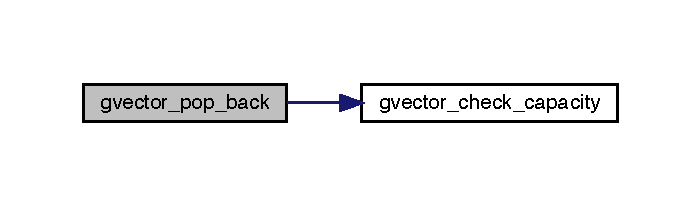
\includegraphics[width=336pt]{group___g_vector_ga6fd765130f11b97b8fcca59d7c4e98d1_cgraph}
\end{center}
\end{figure}
\hypertarget{group___g_vector_ga638f666cc999e6b840302ca1de552b85}{}\label{group___g_vector_ga638f666cc999e6b840302ca1de552b85} 
\index{G\+Vector@{G\+Vector}!gvector\+\_\+push\+\_\+back@{gvector\+\_\+push\+\_\+back}}
\index{gvector\+\_\+push\+\_\+back@{gvector\+\_\+push\+\_\+back}!G\+Vector@{G\+Vector}}
\subsubsection{\texorpdfstring{gvector\+\_\+push\+\_\+back()}{gvector\_push\_back()}}
{\footnotesize\ttfamily void$\ast$ gvector\+\_\+push\+\_\+back (\begin{DoxyParamCaption}\item[{\hyperlink{group___g_vector_ga6d90d5e6b721779a43354f2752b79281}{G\+Vector} $\ast$}]{self,  }\item[{void $\ast$}]{elem }\end{DoxyParamCaption})}



Pushes back a new element to the G\+Vector. Memory reallocation may happen. 


\begin{DoxyParams}{Parameters}
{\em self} & The G\+Vector to access \\
\hline
{\em elem} & Pointer to the element to be copied\\
\hline
\end{DoxyParams}
\begin{DoxyReturn}{Returns}
Pointer to the newly added element 
\end{DoxyReturn}
Here is the call graph for this function\+:\nopagebreak
\begin{figure}[H]
\begin{center}
\leavevmode
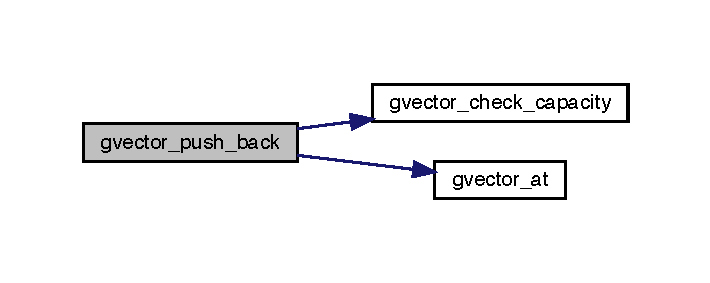
\includegraphics[width=341pt]{group___g_vector_ga638f666cc999e6b840302ca1de552b85_cgraph}
\end{center}
\end{figure}
\hypertarget{group___g_vector_gae4381c0ccdbebaa240e06595e59c5712}{}\label{group___g_vector_gae4381c0ccdbebaa240e06595e59c5712} 
\index{G\+Vector@{G\+Vector}!new\+\_\+gvector@{new\+\_\+gvector}}
\index{new\+\_\+gvector@{new\+\_\+gvector}!G\+Vector@{G\+Vector}}
\subsubsection{\texorpdfstring{new\+\_\+gvector()}{new\_gvector()}}
{\footnotesize\ttfamily \hyperlink{group___g_vector_ga6d90d5e6b721779a43354f2752b79281}{G\+Vector}$\ast$ new\+\_\+gvector (\begin{DoxyParamCaption}\item[{unsigned}]{el\+\_\+size }\end{DoxyParamCaption})}



Constructs a new G\+Vector. 


\begin{DoxyParams}{Parameters}
{\em el\+\_\+size} & Size, in bytes, of the type being stored in this instance of G\+Vector\\
\hline
\end{DoxyParams}
\begin{DoxyReturn}{Returns}
Pointer to the the newly created G\+Vector 
\end{DoxyReturn}

\hypertarget{group___highscores}{}\section{Highscores}
\label{group___highscores}\index{Highscores@{Highscores}}
\subsection*{Classes}
\begin{DoxyCompactItemize}
\item 
struct \hyperlink{struct_score__t}{Score\+\_\+t}
\begin{DoxyCompactList}\small\item\em A structure that contains a score\textquotesingle{}s information. \end{DoxyCompactList}\end{DoxyCompactItemize}
\subsection*{Macros}
\begin{DoxyCompactItemize}
\item 
\#define \hyperlink{group___highscores_gaba51915c87d64af47fb1cc59348961c9}{OK}~0
\item 
\#define \hyperlink{group___highscores_ga1942001a3372417b1fa0106acef995b3}{H\+I\+G\+H\+S\+C\+O\+R\+E\+\_\+\+N\+U\+M\+B\+ER}~5
\begin{DoxyCompactList}\small\item\em Number of high scores saved. \end{DoxyCompactList}\end{DoxyCompactItemize}
\subsection*{Functions}
\begin{DoxyCompactItemize}
\item 
\hyperlink{struct_score__t}{Score\+\_\+t} $\ast$ \hyperlink{group___highscores_ga860a7be33a6a7a627d2fafb624c9631f}{load\+Scores} (const char $\ast$filename)
\begin{DoxyCompactList}\small\item\em Load the 5 Highest Scores from a file into an array. \end{DoxyCompactList}\item 
int \hyperlink{group___highscores_gad0af57912ba7eaec7b5ed3c892b57c10}{write\+Scores} (const char $\ast$filename, \hyperlink{struct_score__t}{Score\+\_\+t} $\ast$scores)
\begin{DoxyCompactList}\small\item\em Writes the 5 Highest Scores from an array into a file. \end{DoxyCompactList}\item 
int \hyperlink{group___highscores_ga8a07ce6e6865afe87235689a394378cc}{update\+Scores} (\hyperlink{struct_score__t}{Score\+\_\+t} $\ast$scores, \hyperlink{struct_score__t}{Score\+\_\+t} newscore)
\begin{DoxyCompactList}\small\item\em Updates the array containing the 5 Highest Scores, with a new Score. \end{DoxyCompactList}\end{DoxyCompactItemize}


\subsection{Detailed Description}
Functions for manipulating the High\+Scores and the files interaction 

\subsection{Macro Definition Documentation}
\hypertarget{group___highscores_ga1942001a3372417b1fa0106acef995b3}{}\label{group___highscores_ga1942001a3372417b1fa0106acef995b3} 
\index{Highscores@{Highscores}!H\+I\+G\+H\+S\+C\+O\+R\+E\+\_\+\+N\+U\+M\+B\+ER@{H\+I\+G\+H\+S\+C\+O\+R\+E\+\_\+\+N\+U\+M\+B\+ER}}
\index{H\+I\+G\+H\+S\+C\+O\+R\+E\+\_\+\+N\+U\+M\+B\+ER@{H\+I\+G\+H\+S\+C\+O\+R\+E\+\_\+\+N\+U\+M\+B\+ER}!Highscores@{Highscores}}
\subsubsection{\texorpdfstring{H\+I\+G\+H\+S\+C\+O\+R\+E\+\_\+\+N\+U\+M\+B\+ER}{HIGHSCORE\_NUMBER}}
{\footnotesize\ttfamily \#define H\+I\+G\+H\+S\+C\+O\+R\+E\+\_\+\+N\+U\+M\+B\+ER~5}



Number of high scores saved. 

\hypertarget{group___highscores_gaba51915c87d64af47fb1cc59348961c9}{}\label{group___highscores_gaba51915c87d64af47fb1cc59348961c9} 
\index{Highscores@{Highscores}!OK@{OK}}
\index{OK@{OK}!Highscores@{Highscores}}
\subsubsection{\texorpdfstring{OK}{OK}}
{\footnotesize\ttfamily \#define OK~0}



\subsection{Function Documentation}
\hypertarget{group___highscores_ga860a7be33a6a7a627d2fafb624c9631f}{}\label{group___highscores_ga860a7be33a6a7a627d2fafb624c9631f} 
\index{Highscores@{Highscores}!load\+Scores@{load\+Scores}}
\index{load\+Scores@{load\+Scores}!Highscores@{Highscores}}
\subsubsection{\texorpdfstring{load\+Scores()}{loadScores()}}
{\footnotesize\ttfamily \hyperlink{struct_score__t}{Score\+\_\+t}$\ast$ load\+Scores (\begin{DoxyParamCaption}\item[{const char $\ast$}]{filename }\end{DoxyParamCaption})}



Load the 5 Highest Scores from a file into an array. 


\begin{DoxyParams}{Parameters}
{\em filename} & path of the location of the file containing the scores\\
\hline
\end{DoxyParams}
\begin{DoxyReturn}{Returns}
Array containg the 5 Highest Scores 
\end{DoxyReturn}
\hypertarget{group___highscores_ga8a07ce6e6865afe87235689a394378cc}{}\label{group___highscores_ga8a07ce6e6865afe87235689a394378cc} 
\index{Highscores@{Highscores}!update\+Scores@{update\+Scores}}
\index{update\+Scores@{update\+Scores}!Highscores@{Highscores}}
\subsubsection{\texorpdfstring{update\+Scores()}{updateScores()}}
{\footnotesize\ttfamily int update\+Scores (\begin{DoxyParamCaption}\item[{\hyperlink{struct_score__t}{Score\+\_\+t} $\ast$}]{scores,  }\item[{\hyperlink{struct_score__t}{Score\+\_\+t}}]{newscore }\end{DoxyParamCaption})}



Updates the array containing the 5 Highest Scores, with a new Score. 

If the Score is not bigger than any of the Highest Scores, the array remains intact.


\begin{DoxyParams}{Parameters}
{\em scores} & Array containing the 5 Highest Scores \\
\hline
{\em newscore} & Score to be added (or not, if not bigger)\\
\hline
\end{DoxyParams}
\begin{DoxyReturn}{Returns}
Return 0 if scores was updated, non-\/zero otherwise 
\end{DoxyReturn}
\hypertarget{group___highscores_gad0af57912ba7eaec7b5ed3c892b57c10}{}\label{group___highscores_gad0af57912ba7eaec7b5ed3c892b57c10} 
\index{Highscores@{Highscores}!write\+Scores@{write\+Scores}}
\index{write\+Scores@{write\+Scores}!Highscores@{Highscores}}
\subsubsection{\texorpdfstring{write\+Scores()}{writeScores()}}
{\footnotesize\ttfamily int write\+Scores (\begin{DoxyParamCaption}\item[{const char $\ast$}]{filename,  }\item[{\hyperlink{struct_score__t}{Score\+\_\+t} $\ast$}]{scores }\end{DoxyParamCaption})}



Writes the 5 Highest Scores from an array into a file. 


\begin{DoxyParams}{Parameters}
{\em filename} & path of the location of the file that is going to be written \\
\hline
{\em scores} & Array containg the Scores that are going to be written\\
\hline
\end{DoxyParams}
\begin{DoxyReturn}{Returns}
Return 0 upon success and non-\/zero otherwise 
\end{DoxyReturn}

\hypertarget{group__i8042}{}\section{i8042}
\label{group__i8042}\index{i8042@{i8042}}
\subsection*{Macros}
\begin{DoxyCompactItemize}
\item 
\#define \hyperlink{group__i8042_ga3a8ea58898cb58fc96013383d39f482c}{B\+IT}(n)~(0x01$<$$<$(n))
\item 
\#define \hyperlink{group__i8042_ga16c5827f043d82f87c726c2d4369c11d}{K\+B\+C\+\_\+\+I\+RQ}~1
\begin{DoxyCompactList}\small\item\em K\+BC I\+RQ line. \end{DoxyCompactList}\item 
\#define \hyperlink{group__i8042_gaa81852ab329dba0e94b98ebcd83fc6f2}{K\+B\+D\+\_\+\+I\+N\+I\+T\+I\+A\+L\+\_\+\+H\+O\+O\+K\+\_\+\+ID}~1
\begin{DoxyCompactList}\small\item\em K\+BD Initial hook\+\_\+id. \end{DoxyCompactList}\item 
\#define \hyperlink{group__i8042_ga592dfdf397b21913348b4dd6b7759b2d}{E\+S\+C\+\_\+\+B\+R\+E\+A\+K\+\_\+\+C\+O\+DE}~0x81
\begin{DoxyCompactList}\small\item\em E\+SC key break code. \end{DoxyCompactList}\item 
\#define \hyperlink{group__i8042_ga54db80d887c9139084b1a66243fa3f72}{E\+N\+T\+E\+R\+\_\+\+B\+R\+E\+A\+K\+\_\+\+C\+O\+DE}~0x9C
\begin{DoxyCompactList}\small\item\em Enter key break code. \end{DoxyCompactList}\item 
\#define \hyperlink{group__i8042_gabfc37fa43c153f929cf0c3421979bfc5}{U\+P\+\_\+\+M\+A\+K\+E\+\_\+\+C\+O\+DE}~0x\+E048
\begin{DoxyCompactList}\small\item\em Up Arrow key make code. \end{DoxyCompactList}\item 
\#define \hyperlink{group__i8042_ga88ccb7cfaafc37d4f31f61191018b4ff}{D\+O\+W\+N\+\_\+\+M\+A\+K\+E\+\_\+\+C\+O\+DE}~0x\+E050
\begin{DoxyCompactList}\small\item\em Down Arrow key make code. \end{DoxyCompactList}\item 
\#define \hyperlink{group__i8042_gacfb42dde389e8ca36ab267002fbf5c6a}{O\+U\+T\+\_\+\+B\+UF}~0x60
\begin{DoxyCompactList}\small\item\em K\+BC Output buffer register. \end{DoxyCompactList}\item 
\#define \hyperlink{group__i8042_ga89c4d098b53809674457b1660b1af780}{S\+T\+A\+T\+\_\+\+R\+EG}~0x64
\begin{DoxyCompactList}\small\item\em K\+BC Status register. \end{DoxyCompactList}\item 
\#define \hyperlink{group__i8042_ga6d57c7927a10f638c83046b52c8caac9}{K\+B\+C\+\_\+\+C\+M\+D\+\_\+\+R\+EG}~0x64
\begin{DoxyCompactList}\small\item\em K\+BC Command register. \end{DoxyCompactList}\item 
\#define \hyperlink{group__i8042_gaac9289c99cf0a693a211da6d6cb1bb65}{K\+B\+C\+\_\+\+I\+N\+\_\+\+B\+UF}~0x60
\begin{DoxyCompactList}\small\item\em K\+BD Input buffer register. \end{DoxyCompactList}\item 
\#define \hyperlink{group__i8042_ga3a22e3be02ba0180834d3c04c03b2640}{S\+T\+A\+T\+\_\+\+P\+A\+R\+I\+TY}~\hyperlink{group___serial_ga3a8ea58898cb58fc96013383d39f482c}{B\+IT}(7)
\item 
\#define \hyperlink{group__i8042_ga0d365c7bae835270c6443e9aa806f503}{S\+T\+A\+T\+\_\+\+T\+I\+M\+E\+O\+UT}~\hyperlink{group___serial_ga3a8ea58898cb58fc96013383d39f482c}{B\+IT}(6)
\item 
\#define \hyperlink{group__i8042_gac38b43e38dfef15c750e716923c66cfe}{S\+T\+A\+T\+\_\+\+A\+UX}~\hyperlink{group___serial_ga3a8ea58898cb58fc96013383d39f482c}{B\+IT}(5)
\item 
\#define \hyperlink{group__i8042_ga5bbeef70f98ceafd4b8c2affbbaa9e97}{S\+T\+A\+T\+\_\+\+I\+NH}~\hyperlink{group___serial_ga3a8ea58898cb58fc96013383d39f482c}{B\+IT}(4)
\item 
\#define \hyperlink{group__i8042_gac284fb8ee0414487d8385d02f288cc4b}{S\+T\+A\+T\+\_\+\+A2}~\hyperlink{group___serial_ga3a8ea58898cb58fc96013383d39f482c}{B\+IT}(3)
\item 
\#define \hyperlink{group__i8042_ga4c990a977bc5fce3f9adcc988fb8cfaf}{S\+T\+A\+T\+\_\+\+S\+YS}~\hyperlink{group___serial_ga3a8ea58898cb58fc96013383d39f482c}{B\+IT}(2)
\item 
\#define \hyperlink{group__i8042_gad4be2937653f616a51e185bdb61343eb}{S\+T\+A\+T\+\_\+\+I\+BF}~\hyperlink{group___serial_ga3a8ea58898cb58fc96013383d39f482c}{B\+IT}(1)
\item 
\#define \hyperlink{group__i8042_ga0ed5883e027c7574b3af486d6cdcbbf9}{S\+T\+A\+T\+\_\+\+O\+BF}~\hyperlink{group___serial_ga3a8ea58898cb58fc96013383d39f482c}{B\+IT}(0)
\item 
\#define \hyperlink{group__i8042_ga3c8f3d570f82da1110d0f57effa3112f}{R\+E\+A\+D\+\_\+\+C\+M\+D\+\_\+B}~0x20
\begin{DoxyCompactList}\small\item\em Read Command Byte. \end{DoxyCompactList}\item 
\#define \hyperlink{group__i8042_ga13e4516a13006d3acfd054edaddb8beb}{W\+R\+I\+T\+E\+\_\+\+C\+M\+D\+\_\+B}~0x60
\begin{DoxyCompactList}\small\item\em Write Command Byte. \end{DoxyCompactList}\item 
\#define \hyperlink{group__i8042_ga55fefff08c94153a53592686472a6c80}{C\+H\+E\+C\+K\+\_\+\+K\+BC}~0x\+AA
\begin{DoxyCompactList}\small\item\em K\+BC Self-\/\+Test. \end{DoxyCompactList}\item 
\#define \hyperlink{group__i8042_ga9d7a05f478671e387655b18be212693a}{C\+H\+E\+C\+K\+\_\+\+K\+B\+D\+\_\+\+I\+FC}~0x\+AB
\begin{DoxyCompactList}\small\item\em Check Keyboard Interface. \end{DoxyCompactList}\item 
\#define \hyperlink{group__i8042_ga816c9396155ea8f3a2e0a6351df3c716}{D\+I\+S\+A\+B\+L\+E\+\_\+\+K\+B\+D\+\_\+\+I\+FC}~0x\+AD
\begin{DoxyCompactList}\small\item\em Disable K\+BD Interface. \end{DoxyCompactList}\item 
\#define \hyperlink{group__i8042_gae8d4fd793912bd5cd0b06e8f69ffe076}{E\+N\+A\+B\+L\+E\+\_\+\+K\+B\+D\+\_\+\+I\+FC}~0x\+AE
\begin{DoxyCompactList}\small\item\em Enable K\+BD Interface. \end{DoxyCompactList}\item 
\#define \hyperlink{group__i8042_ga1cf5a4e33303a3893cc39b330319b1a0}{I\+N\+\_\+\+R\+E\+S\+E\+ND}~0\+X\+FE
\begin{DoxyCompactList}\small\item\em Error\+: Resend latest byte. \end{DoxyCompactList}\item 
\#define \hyperlink{group__i8042_ga975d13d25888550dcf4f69e5a6105cca}{I\+N\+\_\+\+E\+R\+R\+OR}~0\+X\+FC
\begin{DoxyCompactList}\small\item\em Error\+: Restart the entire sequence. \end{DoxyCompactList}\item 
\#define \hyperlink{group__i8042_ga91ac2ffa1978edadfaf6af64fb3e4faf}{I\+N\+\_\+\+A\+CK}~0x\+FA
\begin{DoxyCompactList}\small\item\em Success. \end{DoxyCompactList}\item 
\#define \hyperlink{group__i8042_ga66c64bf8a64b37d06bc7f788583f52ef}{K\+B\+D\+\_\+\+D\+E\+L\+A\+Y\+\_\+\+US}~20000
\begin{DoxyCompactList}\small\item\em K\+BC respond Time-\/\+Out in micro seconds. \end{DoxyCompactList}\end{DoxyCompactItemize}


\subsection{Detailed Description}
Constants for programming the i8042 Keyboard Controller. 

\subsection{Macro Definition Documentation}
\hypertarget{group__i8042_ga3a8ea58898cb58fc96013383d39f482c}{}\label{group__i8042_ga3a8ea58898cb58fc96013383d39f482c} 
\index{i8042@{i8042}!B\+IT@{B\+IT}}
\index{B\+IT@{B\+IT}!i8042@{i8042}}
\subsubsection{\texorpdfstring{B\+IT}{BIT}}
{\footnotesize\ttfamily \#define B\+IT(\begin{DoxyParamCaption}\item[{}]{n }\end{DoxyParamCaption})~(0x01$<$$<$(n))}

\hypertarget{group__i8042_ga55fefff08c94153a53592686472a6c80}{}\label{group__i8042_ga55fefff08c94153a53592686472a6c80} 
\index{i8042@{i8042}!C\+H\+E\+C\+K\+\_\+\+K\+BC@{C\+H\+E\+C\+K\+\_\+\+K\+BC}}
\index{C\+H\+E\+C\+K\+\_\+\+K\+BC@{C\+H\+E\+C\+K\+\_\+\+K\+BC}!i8042@{i8042}}
\subsubsection{\texorpdfstring{C\+H\+E\+C\+K\+\_\+\+K\+BC}{CHECK\_KBC}}
{\footnotesize\ttfamily \#define C\+H\+E\+C\+K\+\_\+\+K\+BC~0x\+AA}



K\+BC Self-\/\+Test. 

\hypertarget{group__i8042_ga9d7a05f478671e387655b18be212693a}{}\label{group__i8042_ga9d7a05f478671e387655b18be212693a} 
\index{i8042@{i8042}!C\+H\+E\+C\+K\+\_\+\+K\+B\+D\+\_\+\+I\+FC@{C\+H\+E\+C\+K\+\_\+\+K\+B\+D\+\_\+\+I\+FC}}
\index{C\+H\+E\+C\+K\+\_\+\+K\+B\+D\+\_\+\+I\+FC@{C\+H\+E\+C\+K\+\_\+\+K\+B\+D\+\_\+\+I\+FC}!i8042@{i8042}}
\subsubsection{\texorpdfstring{C\+H\+E\+C\+K\+\_\+\+K\+B\+D\+\_\+\+I\+FC}{CHECK\_KBD\_IFC}}
{\footnotesize\ttfamily \#define C\+H\+E\+C\+K\+\_\+\+K\+B\+D\+\_\+\+I\+FC~0x\+AB}



Check Keyboard Interface. 

\hypertarget{group__i8042_ga816c9396155ea8f3a2e0a6351df3c716}{}\label{group__i8042_ga816c9396155ea8f3a2e0a6351df3c716} 
\index{i8042@{i8042}!D\+I\+S\+A\+B\+L\+E\+\_\+\+K\+B\+D\+\_\+\+I\+FC@{D\+I\+S\+A\+B\+L\+E\+\_\+\+K\+B\+D\+\_\+\+I\+FC}}
\index{D\+I\+S\+A\+B\+L\+E\+\_\+\+K\+B\+D\+\_\+\+I\+FC@{D\+I\+S\+A\+B\+L\+E\+\_\+\+K\+B\+D\+\_\+\+I\+FC}!i8042@{i8042}}
\subsubsection{\texorpdfstring{D\+I\+S\+A\+B\+L\+E\+\_\+\+K\+B\+D\+\_\+\+I\+FC}{DISABLE\_KBD\_IFC}}
{\footnotesize\ttfamily \#define D\+I\+S\+A\+B\+L\+E\+\_\+\+K\+B\+D\+\_\+\+I\+FC~0x\+AD}



Disable K\+BD Interface. 

\hypertarget{group__i8042_ga88ccb7cfaafc37d4f31f61191018b4ff}{}\label{group__i8042_ga88ccb7cfaafc37d4f31f61191018b4ff} 
\index{i8042@{i8042}!D\+O\+W\+N\+\_\+\+M\+A\+K\+E\+\_\+\+C\+O\+DE@{D\+O\+W\+N\+\_\+\+M\+A\+K\+E\+\_\+\+C\+O\+DE}}
\index{D\+O\+W\+N\+\_\+\+M\+A\+K\+E\+\_\+\+C\+O\+DE@{D\+O\+W\+N\+\_\+\+M\+A\+K\+E\+\_\+\+C\+O\+DE}!i8042@{i8042}}
\subsubsection{\texorpdfstring{D\+O\+W\+N\+\_\+\+M\+A\+K\+E\+\_\+\+C\+O\+DE}{DOWN\_MAKE\_CODE}}
{\footnotesize\ttfamily \#define D\+O\+W\+N\+\_\+\+M\+A\+K\+E\+\_\+\+C\+O\+DE~0x\+E050}



Down Arrow key make code. 

\hypertarget{group__i8042_gae8d4fd793912bd5cd0b06e8f69ffe076}{}\label{group__i8042_gae8d4fd793912bd5cd0b06e8f69ffe076} 
\index{i8042@{i8042}!E\+N\+A\+B\+L\+E\+\_\+\+K\+B\+D\+\_\+\+I\+FC@{E\+N\+A\+B\+L\+E\+\_\+\+K\+B\+D\+\_\+\+I\+FC}}
\index{E\+N\+A\+B\+L\+E\+\_\+\+K\+B\+D\+\_\+\+I\+FC@{E\+N\+A\+B\+L\+E\+\_\+\+K\+B\+D\+\_\+\+I\+FC}!i8042@{i8042}}
\subsubsection{\texorpdfstring{E\+N\+A\+B\+L\+E\+\_\+\+K\+B\+D\+\_\+\+I\+FC}{ENABLE\_KBD\_IFC}}
{\footnotesize\ttfamily \#define E\+N\+A\+B\+L\+E\+\_\+\+K\+B\+D\+\_\+\+I\+FC~0x\+AE}



Enable K\+BD Interface. 

\hypertarget{group__i8042_ga54db80d887c9139084b1a66243fa3f72}{}\label{group__i8042_ga54db80d887c9139084b1a66243fa3f72} 
\index{i8042@{i8042}!E\+N\+T\+E\+R\+\_\+\+B\+R\+E\+A\+K\+\_\+\+C\+O\+DE@{E\+N\+T\+E\+R\+\_\+\+B\+R\+E\+A\+K\+\_\+\+C\+O\+DE}}
\index{E\+N\+T\+E\+R\+\_\+\+B\+R\+E\+A\+K\+\_\+\+C\+O\+DE@{E\+N\+T\+E\+R\+\_\+\+B\+R\+E\+A\+K\+\_\+\+C\+O\+DE}!i8042@{i8042}}
\subsubsection{\texorpdfstring{E\+N\+T\+E\+R\+\_\+\+B\+R\+E\+A\+K\+\_\+\+C\+O\+DE}{ENTER\_BREAK\_CODE}}
{\footnotesize\ttfamily \#define E\+N\+T\+E\+R\+\_\+\+B\+R\+E\+A\+K\+\_\+\+C\+O\+DE~0x9C}



Enter key break code. 

\hypertarget{group__i8042_ga592dfdf397b21913348b4dd6b7759b2d}{}\label{group__i8042_ga592dfdf397b21913348b4dd6b7759b2d} 
\index{i8042@{i8042}!E\+S\+C\+\_\+\+B\+R\+E\+A\+K\+\_\+\+C\+O\+DE@{E\+S\+C\+\_\+\+B\+R\+E\+A\+K\+\_\+\+C\+O\+DE}}
\index{E\+S\+C\+\_\+\+B\+R\+E\+A\+K\+\_\+\+C\+O\+DE@{E\+S\+C\+\_\+\+B\+R\+E\+A\+K\+\_\+\+C\+O\+DE}!i8042@{i8042}}
\subsubsection{\texorpdfstring{E\+S\+C\+\_\+\+B\+R\+E\+A\+K\+\_\+\+C\+O\+DE}{ESC\_BREAK\_CODE}}
{\footnotesize\ttfamily \#define E\+S\+C\+\_\+\+B\+R\+E\+A\+K\+\_\+\+C\+O\+DE~0x81}



E\+SC key break code. 

\hypertarget{group__i8042_ga91ac2ffa1978edadfaf6af64fb3e4faf}{}\label{group__i8042_ga91ac2ffa1978edadfaf6af64fb3e4faf} 
\index{i8042@{i8042}!I\+N\+\_\+\+A\+CK@{I\+N\+\_\+\+A\+CK}}
\index{I\+N\+\_\+\+A\+CK@{I\+N\+\_\+\+A\+CK}!i8042@{i8042}}
\subsubsection{\texorpdfstring{I\+N\+\_\+\+A\+CK}{IN\_ACK}}
{\footnotesize\ttfamily \#define I\+N\+\_\+\+A\+CK~0x\+FA}



Success. 

\hypertarget{group__i8042_ga975d13d25888550dcf4f69e5a6105cca}{}\label{group__i8042_ga975d13d25888550dcf4f69e5a6105cca} 
\index{i8042@{i8042}!I\+N\+\_\+\+E\+R\+R\+OR@{I\+N\+\_\+\+E\+R\+R\+OR}}
\index{I\+N\+\_\+\+E\+R\+R\+OR@{I\+N\+\_\+\+E\+R\+R\+OR}!i8042@{i8042}}
\subsubsection{\texorpdfstring{I\+N\+\_\+\+E\+R\+R\+OR}{IN\_ERROR}}
{\footnotesize\ttfamily \#define I\+N\+\_\+\+E\+R\+R\+OR~0\+X\+FC}



Error\+: Restart the entire sequence. 

\hypertarget{group__i8042_ga1cf5a4e33303a3893cc39b330319b1a0}{}\label{group__i8042_ga1cf5a4e33303a3893cc39b330319b1a0} 
\index{i8042@{i8042}!I\+N\+\_\+\+R\+E\+S\+E\+ND@{I\+N\+\_\+\+R\+E\+S\+E\+ND}}
\index{I\+N\+\_\+\+R\+E\+S\+E\+ND@{I\+N\+\_\+\+R\+E\+S\+E\+ND}!i8042@{i8042}}
\subsubsection{\texorpdfstring{I\+N\+\_\+\+R\+E\+S\+E\+ND}{IN\_RESEND}}
{\footnotesize\ttfamily \#define I\+N\+\_\+\+R\+E\+S\+E\+ND~0\+X\+FE}



Error\+: Resend latest byte. 

K\+BD Responses to Inputs \hypertarget{group__i8042_ga6d57c7927a10f638c83046b52c8caac9}{}\label{group__i8042_ga6d57c7927a10f638c83046b52c8caac9} 
\index{i8042@{i8042}!K\+B\+C\+\_\+\+C\+M\+D\+\_\+\+R\+EG@{K\+B\+C\+\_\+\+C\+M\+D\+\_\+\+R\+EG}}
\index{K\+B\+C\+\_\+\+C\+M\+D\+\_\+\+R\+EG@{K\+B\+C\+\_\+\+C\+M\+D\+\_\+\+R\+EG}!i8042@{i8042}}
\subsubsection{\texorpdfstring{K\+B\+C\+\_\+\+C\+M\+D\+\_\+\+R\+EG}{KBC\_CMD\_REG}}
{\footnotesize\ttfamily \#define K\+B\+C\+\_\+\+C\+M\+D\+\_\+\+R\+EG~0x64}



K\+BC Command register. 

\hypertarget{group__i8042_gaac9289c99cf0a693a211da6d6cb1bb65}{}\label{group__i8042_gaac9289c99cf0a693a211da6d6cb1bb65} 
\index{i8042@{i8042}!K\+B\+C\+\_\+\+I\+N\+\_\+\+B\+UF@{K\+B\+C\+\_\+\+I\+N\+\_\+\+B\+UF}}
\index{K\+B\+C\+\_\+\+I\+N\+\_\+\+B\+UF@{K\+B\+C\+\_\+\+I\+N\+\_\+\+B\+UF}!i8042@{i8042}}
\subsubsection{\texorpdfstring{K\+B\+C\+\_\+\+I\+N\+\_\+\+B\+UF}{KBC\_IN\_BUF}}
{\footnotesize\ttfamily \#define K\+B\+C\+\_\+\+I\+N\+\_\+\+B\+UF~0x60}



K\+BD Input buffer register. 

\hypertarget{group__i8042_ga16c5827f043d82f87c726c2d4369c11d}{}\label{group__i8042_ga16c5827f043d82f87c726c2d4369c11d} 
\index{i8042@{i8042}!K\+B\+C\+\_\+\+I\+RQ@{K\+B\+C\+\_\+\+I\+RQ}}
\index{K\+B\+C\+\_\+\+I\+RQ@{K\+B\+C\+\_\+\+I\+RQ}!i8042@{i8042}}
\subsubsection{\texorpdfstring{K\+B\+C\+\_\+\+I\+RQ}{KBC\_IRQ}}
{\footnotesize\ttfamily \#define K\+B\+C\+\_\+\+I\+RQ~1}



K\+BC I\+RQ line. 

\hypertarget{group__i8042_ga66c64bf8a64b37d06bc7f788583f52ef}{}\label{group__i8042_ga66c64bf8a64b37d06bc7f788583f52ef} 
\index{i8042@{i8042}!K\+B\+D\+\_\+\+D\+E\+L\+A\+Y\+\_\+\+US@{K\+B\+D\+\_\+\+D\+E\+L\+A\+Y\+\_\+\+US}}
\index{K\+B\+D\+\_\+\+D\+E\+L\+A\+Y\+\_\+\+US@{K\+B\+D\+\_\+\+D\+E\+L\+A\+Y\+\_\+\+US}!i8042@{i8042}}
\subsubsection{\texorpdfstring{K\+B\+D\+\_\+\+D\+E\+L\+A\+Y\+\_\+\+US}{KBD\_DELAY\_US}}
{\footnotesize\ttfamily \#define K\+B\+D\+\_\+\+D\+E\+L\+A\+Y\+\_\+\+US~20000}



K\+BC respond Time-\/\+Out in micro seconds. 

\hypertarget{group__i8042_gaa81852ab329dba0e94b98ebcd83fc6f2}{}\label{group__i8042_gaa81852ab329dba0e94b98ebcd83fc6f2} 
\index{i8042@{i8042}!K\+B\+D\+\_\+\+I\+N\+I\+T\+I\+A\+L\+\_\+\+H\+O\+O\+K\+\_\+\+ID@{K\+B\+D\+\_\+\+I\+N\+I\+T\+I\+A\+L\+\_\+\+H\+O\+O\+K\+\_\+\+ID}}
\index{K\+B\+D\+\_\+\+I\+N\+I\+T\+I\+A\+L\+\_\+\+H\+O\+O\+K\+\_\+\+ID@{K\+B\+D\+\_\+\+I\+N\+I\+T\+I\+A\+L\+\_\+\+H\+O\+O\+K\+\_\+\+ID}!i8042@{i8042}}
\subsubsection{\texorpdfstring{K\+B\+D\+\_\+\+I\+N\+I\+T\+I\+A\+L\+\_\+\+H\+O\+O\+K\+\_\+\+ID}{KBD\_INITIAL\_HOOK\_ID}}
{\footnotesize\ttfamily \#define K\+B\+D\+\_\+\+I\+N\+I\+T\+I\+A\+L\+\_\+\+H\+O\+O\+K\+\_\+\+ID~1}



K\+BD Initial hook\+\_\+id. 

\hypertarget{group__i8042_gacfb42dde389e8ca36ab267002fbf5c6a}{}\label{group__i8042_gacfb42dde389e8ca36ab267002fbf5c6a} 
\index{i8042@{i8042}!O\+U\+T\+\_\+\+B\+UF@{O\+U\+T\+\_\+\+B\+UF}}
\index{O\+U\+T\+\_\+\+B\+UF@{O\+U\+T\+\_\+\+B\+UF}!i8042@{i8042}}
\subsubsection{\texorpdfstring{O\+U\+T\+\_\+\+B\+UF}{OUT\_BUF}}
{\footnotesize\ttfamily \#define O\+U\+T\+\_\+\+B\+UF~0x60}



K\+BC Output buffer register. 

I\+N\+P\+U\+T\+\_\+\+B\+U\+F\+F\+ER is accessed by ports 0x60 or 0x64, depending on context \hypertarget{group__i8042_ga3c8f3d570f82da1110d0f57effa3112f}{}\label{group__i8042_ga3c8f3d570f82da1110d0f57effa3112f} 
\index{i8042@{i8042}!R\+E\+A\+D\+\_\+\+C\+M\+D\+\_\+B@{R\+E\+A\+D\+\_\+\+C\+M\+D\+\_\+B}}
\index{R\+E\+A\+D\+\_\+\+C\+M\+D\+\_\+B@{R\+E\+A\+D\+\_\+\+C\+M\+D\+\_\+B}!i8042@{i8042}}
\subsubsection{\texorpdfstring{R\+E\+A\+D\+\_\+\+C\+M\+D\+\_\+B}{READ\_CMD\_B}}
{\footnotesize\ttfamily \#define R\+E\+A\+D\+\_\+\+C\+M\+D\+\_\+B~0x20}



Read Command Byte. 

K\+BD Commands for P\+C-\/\+AT \hypertarget{group__i8042_gac284fb8ee0414487d8385d02f288cc4b}{}\label{group__i8042_gac284fb8ee0414487d8385d02f288cc4b} 
\index{i8042@{i8042}!S\+T\+A\+T\+\_\+\+A2@{S\+T\+A\+T\+\_\+\+A2}}
\index{S\+T\+A\+T\+\_\+\+A2@{S\+T\+A\+T\+\_\+\+A2}!i8042@{i8042}}
\subsubsection{\texorpdfstring{S\+T\+A\+T\+\_\+\+A2}{STAT\_A2}}
{\footnotesize\ttfamily \#define S\+T\+A\+T\+\_\+\+A2~\hyperlink{group___serial_ga3a8ea58898cb58fc96013383d39f482c}{B\+IT}(3)}

\hypertarget{group__i8042_gac38b43e38dfef15c750e716923c66cfe}{}\label{group__i8042_gac38b43e38dfef15c750e716923c66cfe} 
\index{i8042@{i8042}!S\+T\+A\+T\+\_\+\+A\+UX@{S\+T\+A\+T\+\_\+\+A\+UX}}
\index{S\+T\+A\+T\+\_\+\+A\+UX@{S\+T\+A\+T\+\_\+\+A\+UX}!i8042@{i8042}}
\subsubsection{\texorpdfstring{S\+T\+A\+T\+\_\+\+A\+UX}{STAT\_AUX}}
{\footnotesize\ttfamily \#define S\+T\+A\+T\+\_\+\+A\+UX~\hyperlink{group___serial_ga3a8ea58898cb58fc96013383d39f482c}{B\+IT}(5)}

\hypertarget{group__i8042_gad4be2937653f616a51e185bdb61343eb}{}\label{group__i8042_gad4be2937653f616a51e185bdb61343eb} 
\index{i8042@{i8042}!S\+T\+A\+T\+\_\+\+I\+BF@{S\+T\+A\+T\+\_\+\+I\+BF}}
\index{S\+T\+A\+T\+\_\+\+I\+BF@{S\+T\+A\+T\+\_\+\+I\+BF}!i8042@{i8042}}
\subsubsection{\texorpdfstring{S\+T\+A\+T\+\_\+\+I\+BF}{STAT\_IBF}}
{\footnotesize\ttfamily \#define S\+T\+A\+T\+\_\+\+I\+BF~\hyperlink{group___serial_ga3a8ea58898cb58fc96013383d39f482c}{B\+IT}(1)}

\hypertarget{group__i8042_ga5bbeef70f98ceafd4b8c2affbbaa9e97}{}\label{group__i8042_ga5bbeef70f98ceafd4b8c2affbbaa9e97} 
\index{i8042@{i8042}!S\+T\+A\+T\+\_\+\+I\+NH@{S\+T\+A\+T\+\_\+\+I\+NH}}
\index{S\+T\+A\+T\+\_\+\+I\+NH@{S\+T\+A\+T\+\_\+\+I\+NH}!i8042@{i8042}}
\subsubsection{\texorpdfstring{S\+T\+A\+T\+\_\+\+I\+NH}{STAT\_INH}}
{\footnotesize\ttfamily \#define S\+T\+A\+T\+\_\+\+I\+NH~\hyperlink{group___serial_ga3a8ea58898cb58fc96013383d39f482c}{B\+IT}(4)}

\hypertarget{group__i8042_ga0ed5883e027c7574b3af486d6cdcbbf9}{}\label{group__i8042_ga0ed5883e027c7574b3af486d6cdcbbf9} 
\index{i8042@{i8042}!S\+T\+A\+T\+\_\+\+O\+BF@{S\+T\+A\+T\+\_\+\+O\+BF}}
\index{S\+T\+A\+T\+\_\+\+O\+BF@{S\+T\+A\+T\+\_\+\+O\+BF}!i8042@{i8042}}
\subsubsection{\texorpdfstring{S\+T\+A\+T\+\_\+\+O\+BF}{STAT\_OBF}}
{\footnotesize\ttfamily \#define S\+T\+A\+T\+\_\+\+O\+BF~\hyperlink{group___serial_ga3a8ea58898cb58fc96013383d39f482c}{B\+IT}(0)}

\hypertarget{group__i8042_ga3a22e3be02ba0180834d3c04c03b2640}{}\label{group__i8042_ga3a22e3be02ba0180834d3c04c03b2640} 
\index{i8042@{i8042}!S\+T\+A\+T\+\_\+\+P\+A\+R\+I\+TY@{S\+T\+A\+T\+\_\+\+P\+A\+R\+I\+TY}}
\index{S\+T\+A\+T\+\_\+\+P\+A\+R\+I\+TY@{S\+T\+A\+T\+\_\+\+P\+A\+R\+I\+TY}!i8042@{i8042}}
\subsubsection{\texorpdfstring{S\+T\+A\+T\+\_\+\+P\+A\+R\+I\+TY}{STAT\_PARITY}}
{\footnotesize\ttfamily \#define S\+T\+A\+T\+\_\+\+P\+A\+R\+I\+TY~\hyperlink{group___serial_ga3a8ea58898cb58fc96013383d39f482c}{B\+IT}(7)}

K\+BC Status Register B\+I\+Ts\textquotesingle{} Meaning \hypertarget{group__i8042_ga89c4d098b53809674457b1660b1af780}{}\label{group__i8042_ga89c4d098b53809674457b1660b1af780} 
\index{i8042@{i8042}!S\+T\+A\+T\+\_\+\+R\+EG@{S\+T\+A\+T\+\_\+\+R\+EG}}
\index{S\+T\+A\+T\+\_\+\+R\+EG@{S\+T\+A\+T\+\_\+\+R\+EG}!i8042@{i8042}}
\subsubsection{\texorpdfstring{S\+T\+A\+T\+\_\+\+R\+EG}{STAT\_REG}}
{\footnotesize\ttfamily \#define S\+T\+A\+T\+\_\+\+R\+EG~0x64}



K\+BC Status register. 

\hypertarget{group__i8042_ga4c990a977bc5fce3f9adcc988fb8cfaf}{}\label{group__i8042_ga4c990a977bc5fce3f9adcc988fb8cfaf} 
\index{i8042@{i8042}!S\+T\+A\+T\+\_\+\+S\+YS@{S\+T\+A\+T\+\_\+\+S\+YS}}
\index{S\+T\+A\+T\+\_\+\+S\+YS@{S\+T\+A\+T\+\_\+\+S\+YS}!i8042@{i8042}}
\subsubsection{\texorpdfstring{S\+T\+A\+T\+\_\+\+S\+YS}{STAT\_SYS}}
{\footnotesize\ttfamily \#define S\+T\+A\+T\+\_\+\+S\+YS~\hyperlink{group___serial_ga3a8ea58898cb58fc96013383d39f482c}{B\+IT}(2)}

\hypertarget{group__i8042_ga0d365c7bae835270c6443e9aa806f503}{}\label{group__i8042_ga0d365c7bae835270c6443e9aa806f503} 
\index{i8042@{i8042}!S\+T\+A\+T\+\_\+\+T\+I\+M\+E\+O\+UT@{S\+T\+A\+T\+\_\+\+T\+I\+M\+E\+O\+UT}}
\index{S\+T\+A\+T\+\_\+\+T\+I\+M\+E\+O\+UT@{S\+T\+A\+T\+\_\+\+T\+I\+M\+E\+O\+UT}!i8042@{i8042}}
\subsubsection{\texorpdfstring{S\+T\+A\+T\+\_\+\+T\+I\+M\+E\+O\+UT}{STAT\_TIMEOUT}}
{\footnotesize\ttfamily \#define S\+T\+A\+T\+\_\+\+T\+I\+M\+E\+O\+UT~\hyperlink{group___serial_ga3a8ea58898cb58fc96013383d39f482c}{B\+IT}(6)}

\hypertarget{group__i8042_gabfc37fa43c153f929cf0c3421979bfc5}{}\label{group__i8042_gabfc37fa43c153f929cf0c3421979bfc5} 
\index{i8042@{i8042}!U\+P\+\_\+\+M\+A\+K\+E\+\_\+\+C\+O\+DE@{U\+P\+\_\+\+M\+A\+K\+E\+\_\+\+C\+O\+DE}}
\index{U\+P\+\_\+\+M\+A\+K\+E\+\_\+\+C\+O\+DE@{U\+P\+\_\+\+M\+A\+K\+E\+\_\+\+C\+O\+DE}!i8042@{i8042}}
\subsubsection{\texorpdfstring{U\+P\+\_\+\+M\+A\+K\+E\+\_\+\+C\+O\+DE}{UP\_MAKE\_CODE}}
{\footnotesize\ttfamily \#define U\+P\+\_\+\+M\+A\+K\+E\+\_\+\+C\+O\+DE~0x\+E048}



Up Arrow key make code. 

\hypertarget{group__i8042_ga13e4516a13006d3acfd054edaddb8beb}{}\label{group__i8042_ga13e4516a13006d3acfd054edaddb8beb} 
\index{i8042@{i8042}!W\+R\+I\+T\+E\+\_\+\+C\+M\+D\+\_\+B@{W\+R\+I\+T\+E\+\_\+\+C\+M\+D\+\_\+B}}
\index{W\+R\+I\+T\+E\+\_\+\+C\+M\+D\+\_\+B@{W\+R\+I\+T\+E\+\_\+\+C\+M\+D\+\_\+B}!i8042@{i8042}}
\subsubsection{\texorpdfstring{W\+R\+I\+T\+E\+\_\+\+C\+M\+D\+\_\+B}{WRITE\_CMD\_B}}
{\footnotesize\ttfamily \#define W\+R\+I\+T\+E\+\_\+\+C\+M\+D\+\_\+B~0x60}



Write Command Byte. 


\hypertarget{group__i8254}{}\section{i8254}
\label{group__i8254}\index{i8254@{i8254}}
\subsection*{Macros}
\begin{DoxyCompactItemize}
\item 
\#define \hyperlink{group__i8254_gacf926951944b6cf370b7229ebd50dd8b}{T\+I\+M\+E\+R\+\_\+\+F\+R\+EQ}~1193182
\begin{DoxyCompactList}\small\item\em clock frequency for timer in PC and AT \end{DoxyCompactList}\item 
\#define \hyperlink{group__i8254_ga3a8ea58898cb58fc96013383d39f482c}{B\+IT}(n)~(0x01$<$$<$(n))
\item 
\#define \hyperlink{group__i8254_ga30bf84c312af248cb81bb224e09f9ba8}{T\+I\+M\+E\+R0\+\_\+\+I\+RQ}~0
\begin{DoxyCompactList}\small\item\em Timer 0 I\+RQ line. \end{DoxyCompactList}\item 
\#define \hyperlink{group__i8254_ga5a49703fe985c8df41c3be0ed091ac45}{T\+I\+M\+E\+R0\+\_\+\+I\+R\+Q\+S\+ET}~0
\begin{DoxyCompactList}\small\item\em Timer 0 Policy Bit. \end{DoxyCompactList}\item 
\#define \hyperlink{group__i8254_gacc9ff9df4a9674a1ce9ba08fc4a4679e}{T\+I\+M\+E\+R\+\_\+0}~0x40
\begin{DoxyCompactList}\small\item\em Timer 0 count register. \end{DoxyCompactList}\item 
\#define \hyperlink{group__i8254_gac62c99c2a9289891c1b83052242cca49}{T\+I\+M\+E\+R\+\_\+1}~0x41
\begin{DoxyCompactList}\small\item\em Timer 1 count register. \end{DoxyCompactList}\item 
\#define \hyperlink{group__i8254_ga1f34f18ad0ab8cace46b615773b48735}{T\+I\+M\+E\+R\+\_\+2}~0x42
\begin{DoxyCompactList}\small\item\em Timer 2 count register. \end{DoxyCompactList}\item 
\#define \hyperlink{group__i8254_ga282832448fb0281ef53d243c1cd48491}{T\+I\+M\+E\+R\+\_\+\+C\+T\+RL}~0x43
\begin{DoxyCompactList}\small\item\em Control register. \end{DoxyCompactList}\item 
\#define \hyperlink{group__i8254_ga51b3a5e3d4811ca063fe25e35560ab40}{S\+P\+E\+A\+K\+E\+R\+\_\+\+C\+T\+RL}~0x61
\begin{DoxyCompactList}\small\item\em Register for speaker control. \end{DoxyCompactList}\item 
\#define \hyperlink{group__i8254_ga6a4822642d40c248435692324a818010}{T\+I\+M\+E\+R\+\_\+\+S\+E\+L0}~0x00
\begin{DoxyCompactList}\small\item\em Control Word for Timer 0. \end{DoxyCompactList}\item 
\#define \hyperlink{group__i8254_ga8349623fd8d99f9cc5d8ae29d78594fc}{T\+I\+M\+E\+R\+\_\+\+S\+E\+L1}~\hyperlink{group___serial_ga3a8ea58898cb58fc96013383d39f482c}{B\+IT}(6)
\begin{DoxyCompactList}\small\item\em Control Word for Timer 1. \end{DoxyCompactList}\item 
\#define \hyperlink{group__i8254_ga142a255de0dbc48aeabd45fc10c33672}{T\+I\+M\+E\+R\+\_\+\+S\+E\+L2}~\hyperlink{group___serial_ga3a8ea58898cb58fc96013383d39f482c}{B\+IT}(7)
\begin{DoxyCompactList}\small\item\em Control Word for Timer 2. \end{DoxyCompactList}\item 
\#define \hyperlink{group__i8254_ga4c2eecbfb96744a9c2af71dba75ecb18}{T\+I\+M\+E\+R\+\_\+\+R\+B\+\_\+\+C\+MD}~(\hyperlink{group___serial_ga3a8ea58898cb58fc96013383d39f482c}{B\+IT}(7)$\vert$\hyperlink{group___serial_ga3a8ea58898cb58fc96013383d39f482c}{B\+IT}(6))
\begin{DoxyCompactList}\small\item\em Read Back Command. \end{DoxyCompactList}\item 
\#define \hyperlink{group__i8254_gac18cb814ebd0d67235392c330e0e3504}{T\+I\+M\+E\+R\+\_\+\+L\+SB}~\hyperlink{group___serial_ga3a8ea58898cb58fc96013383d39f482c}{B\+IT}(4)
\begin{DoxyCompactList}\small\item\em Initialize Counter L\+SB only. \end{DoxyCompactList}\item 
\#define \hyperlink{group__i8254_ga2a8a6d363c612d756cd8d78480f7cd04}{T\+I\+M\+E\+R\+\_\+\+M\+SB}~\hyperlink{group___serial_ga3a8ea58898cb58fc96013383d39f482c}{B\+IT}(5)
\begin{DoxyCompactList}\small\item\em Initialize Counter M\+SB only. \end{DoxyCompactList}\item 
\#define \hyperlink{group__i8254_ga8c0f1933323274c765e23837e4fbc8c7}{T\+I\+M\+E\+R\+\_\+\+L\+S\+B\+\_\+\+M\+SB}~(\hyperlink{group__i8254_gac18cb814ebd0d67235392c330e0e3504}{T\+I\+M\+E\+R\+\_\+\+L\+SB} $\vert$ \hyperlink{group__i8254_ga2a8a6d363c612d756cd8d78480f7cd04}{T\+I\+M\+E\+R\+\_\+\+M\+SB})
\begin{DoxyCompactList}\small\item\em Initialize L\+SB first and M\+SB afterwards. \end{DoxyCompactList}\item 
\#define \hyperlink{group__i8254_ga4745cbf21da3d3fea5dbb080b2b73bac}{T\+I\+M\+E\+R\+\_\+\+S\+Q\+R\+\_\+\+W\+A\+VE}~(\hyperlink{group___serial_ga3a8ea58898cb58fc96013383d39f482c}{B\+IT}(2)$\vert$\hyperlink{group___serial_ga3a8ea58898cb58fc96013383d39f482c}{B\+IT}(1))
\begin{DoxyCompactList}\small\item\em Mode 3\+: square wave generator. \end{DoxyCompactList}\item 
\#define \hyperlink{group__i8254_ga5d4449e0fa1cf4a4d107a48a04a1265f}{T\+I\+M\+E\+R\+\_\+\+R\+A\+T\+E\+\_\+\+G\+EN}~\hyperlink{group___serial_ga3a8ea58898cb58fc96013383d39f482c}{B\+IT}(2)
\begin{DoxyCompactList}\small\item\em Mode 2\+: rate generator. \end{DoxyCompactList}\item 
\#define \hyperlink{group__i8254_ga325b992a371d5d981c4eceff42fa5956}{T\+I\+M\+E\+R\+\_\+\+B\+CD}~0x01
\begin{DoxyCompactList}\small\item\em Count in B\+CD. \end{DoxyCompactList}\item 
\#define \hyperlink{group__i8254_gad2913dcf2f91453317bd035589ac0a7d}{T\+I\+M\+E\+R\+\_\+\+B\+IN}~0x00
\begin{DoxyCompactList}\small\item\em Count in binary. \end{DoxyCompactList}\item 
\#define \hyperlink{group__i8254_ga6c248216df24b5e9d907d126d80bd195}{T\+I\+M\+E\+R\+\_\+\+R\+B\+\_\+\+C\+O\+U\+N\+T\+\_\+}~\hyperlink{group___serial_ga3a8ea58898cb58fc96013383d39f482c}{B\+IT}(5)
\item 
\#define \hyperlink{group__i8254_ga08b4952bb7058684a3f8f66be04dd45e}{T\+I\+M\+E\+R\+\_\+\+R\+B\+\_\+\+S\+T\+A\+T\+U\+S\+\_\+}~\hyperlink{group___serial_ga3a8ea58898cb58fc96013383d39f482c}{B\+IT}(4)
\item 
\#define \hyperlink{group__i8254_gaf598b17740e07842a0545af512714711}{T\+I\+M\+E\+R\+\_\+\+R\+B\+\_\+\+S\+EL}(n)~\hyperlink{group___serial_ga3a8ea58898cb58fc96013383d39f482c}{B\+IT}((n)+1)
\end{DoxyCompactItemize}


\subsection{Detailed Description}
Constants for programming the i8254 Timer. Needs to be completed. 

\subsection{Macro Definition Documentation}
\hypertarget{group__i8254_ga3a8ea58898cb58fc96013383d39f482c}{}\label{group__i8254_ga3a8ea58898cb58fc96013383d39f482c} 
\index{i8254@{i8254}!B\+IT@{B\+IT}}
\index{B\+IT@{B\+IT}!i8254@{i8254}}
\subsubsection{\texorpdfstring{B\+IT}{BIT}}
{\footnotesize\ttfamily \#define B\+IT(\begin{DoxyParamCaption}\item[{}]{n }\end{DoxyParamCaption})~(0x01$<$$<$(n))}

\hypertarget{group__i8254_ga51b3a5e3d4811ca063fe25e35560ab40}{}\label{group__i8254_ga51b3a5e3d4811ca063fe25e35560ab40} 
\index{i8254@{i8254}!S\+P\+E\+A\+K\+E\+R\+\_\+\+C\+T\+RL@{S\+P\+E\+A\+K\+E\+R\+\_\+\+C\+T\+RL}}
\index{S\+P\+E\+A\+K\+E\+R\+\_\+\+C\+T\+RL@{S\+P\+E\+A\+K\+E\+R\+\_\+\+C\+T\+RL}!i8254@{i8254}}
\subsubsection{\texorpdfstring{S\+P\+E\+A\+K\+E\+R\+\_\+\+C\+T\+RL}{SPEAKER\_CTRL}}
{\footnotesize\ttfamily \#define S\+P\+E\+A\+K\+E\+R\+\_\+\+C\+T\+RL~0x61}



Register for speaker control. 

\hypertarget{group__i8254_ga30bf84c312af248cb81bb224e09f9ba8}{}\label{group__i8254_ga30bf84c312af248cb81bb224e09f9ba8} 
\index{i8254@{i8254}!T\+I\+M\+E\+R0\+\_\+\+I\+RQ@{T\+I\+M\+E\+R0\+\_\+\+I\+RQ}}
\index{T\+I\+M\+E\+R0\+\_\+\+I\+RQ@{T\+I\+M\+E\+R0\+\_\+\+I\+RQ}!i8254@{i8254}}
\subsubsection{\texorpdfstring{T\+I\+M\+E\+R0\+\_\+\+I\+RQ}{TIMER0\_IRQ}}
{\footnotesize\ttfamily \#define T\+I\+M\+E\+R0\+\_\+\+I\+RQ~0}



Timer 0 I\+RQ line. 

\hypertarget{group__i8254_ga5a49703fe985c8df41c3be0ed091ac45}{}\label{group__i8254_ga5a49703fe985c8df41c3be0ed091ac45} 
\index{i8254@{i8254}!T\+I\+M\+E\+R0\+\_\+\+I\+R\+Q\+S\+ET@{T\+I\+M\+E\+R0\+\_\+\+I\+R\+Q\+S\+ET}}
\index{T\+I\+M\+E\+R0\+\_\+\+I\+R\+Q\+S\+ET@{T\+I\+M\+E\+R0\+\_\+\+I\+R\+Q\+S\+ET}!i8254@{i8254}}
\subsubsection{\texorpdfstring{T\+I\+M\+E\+R0\+\_\+\+I\+R\+Q\+S\+ET}{TIMER0\_IRQSET}}
{\footnotesize\ttfamily \#define T\+I\+M\+E\+R0\+\_\+\+I\+R\+Q\+S\+ET~0}



Timer 0 Policy Bit. 

\hypertarget{group__i8254_gacc9ff9df4a9674a1ce9ba08fc4a4679e}{}\label{group__i8254_gacc9ff9df4a9674a1ce9ba08fc4a4679e} 
\index{i8254@{i8254}!T\+I\+M\+E\+R\+\_\+0@{T\+I\+M\+E\+R\+\_\+0}}
\index{T\+I\+M\+E\+R\+\_\+0@{T\+I\+M\+E\+R\+\_\+0}!i8254@{i8254}}
\subsubsection{\texorpdfstring{T\+I\+M\+E\+R\+\_\+0}{TIMER\_0}}
{\footnotesize\ttfamily \#define T\+I\+M\+E\+R\+\_\+0~0x40}



Timer 0 count register. 

I/O port addresses \hypertarget{group__i8254_gac62c99c2a9289891c1b83052242cca49}{}\label{group__i8254_gac62c99c2a9289891c1b83052242cca49} 
\index{i8254@{i8254}!T\+I\+M\+E\+R\+\_\+1@{T\+I\+M\+E\+R\+\_\+1}}
\index{T\+I\+M\+E\+R\+\_\+1@{T\+I\+M\+E\+R\+\_\+1}!i8254@{i8254}}
\subsubsection{\texorpdfstring{T\+I\+M\+E\+R\+\_\+1}{TIMER\_1}}
{\footnotesize\ttfamily \#define T\+I\+M\+E\+R\+\_\+1~0x41}



Timer 1 count register. 

\hypertarget{group__i8254_ga1f34f18ad0ab8cace46b615773b48735}{}\label{group__i8254_ga1f34f18ad0ab8cace46b615773b48735} 
\index{i8254@{i8254}!T\+I\+M\+E\+R\+\_\+2@{T\+I\+M\+E\+R\+\_\+2}}
\index{T\+I\+M\+E\+R\+\_\+2@{T\+I\+M\+E\+R\+\_\+2}!i8254@{i8254}}
\subsubsection{\texorpdfstring{T\+I\+M\+E\+R\+\_\+2}{TIMER\_2}}
{\footnotesize\ttfamily \#define T\+I\+M\+E\+R\+\_\+2~0x42}



Timer 2 count register. 

\hypertarget{group__i8254_ga325b992a371d5d981c4eceff42fa5956}{}\label{group__i8254_ga325b992a371d5d981c4eceff42fa5956} 
\index{i8254@{i8254}!T\+I\+M\+E\+R\+\_\+\+B\+CD@{T\+I\+M\+E\+R\+\_\+\+B\+CD}}
\index{T\+I\+M\+E\+R\+\_\+\+B\+CD@{T\+I\+M\+E\+R\+\_\+\+B\+CD}!i8254@{i8254}}
\subsubsection{\texorpdfstring{T\+I\+M\+E\+R\+\_\+\+B\+CD}{TIMER\_BCD}}
{\footnotesize\ttfamily \#define T\+I\+M\+E\+R\+\_\+\+B\+CD~0x01}



Count in B\+CD. 

Counting mode\+: bit 0 \hypertarget{group__i8254_gad2913dcf2f91453317bd035589ac0a7d}{}\label{group__i8254_gad2913dcf2f91453317bd035589ac0a7d} 
\index{i8254@{i8254}!T\+I\+M\+E\+R\+\_\+\+B\+IN@{T\+I\+M\+E\+R\+\_\+\+B\+IN}}
\index{T\+I\+M\+E\+R\+\_\+\+B\+IN@{T\+I\+M\+E\+R\+\_\+\+B\+IN}!i8254@{i8254}}
\subsubsection{\texorpdfstring{T\+I\+M\+E\+R\+\_\+\+B\+IN}{TIMER\_BIN}}
{\footnotesize\ttfamily \#define T\+I\+M\+E\+R\+\_\+\+B\+IN~0x00}



Count in binary. 

\hypertarget{group__i8254_ga282832448fb0281ef53d243c1cd48491}{}\label{group__i8254_ga282832448fb0281ef53d243c1cd48491} 
\index{i8254@{i8254}!T\+I\+M\+E\+R\+\_\+\+C\+T\+RL@{T\+I\+M\+E\+R\+\_\+\+C\+T\+RL}}
\index{T\+I\+M\+E\+R\+\_\+\+C\+T\+RL@{T\+I\+M\+E\+R\+\_\+\+C\+T\+RL}!i8254@{i8254}}
\subsubsection{\texorpdfstring{T\+I\+M\+E\+R\+\_\+\+C\+T\+RL}{TIMER\_CTRL}}
{\footnotesize\ttfamily \#define T\+I\+M\+E\+R\+\_\+\+C\+T\+RL~0x43}



Control register. 

\hypertarget{group__i8254_gacf926951944b6cf370b7229ebd50dd8b}{}\label{group__i8254_gacf926951944b6cf370b7229ebd50dd8b} 
\index{i8254@{i8254}!T\+I\+M\+E\+R\+\_\+\+F\+R\+EQ@{T\+I\+M\+E\+R\+\_\+\+F\+R\+EQ}}
\index{T\+I\+M\+E\+R\+\_\+\+F\+R\+EQ@{T\+I\+M\+E\+R\+\_\+\+F\+R\+EQ}!i8254@{i8254}}
\subsubsection{\texorpdfstring{T\+I\+M\+E\+R\+\_\+\+F\+R\+EQ}{TIMER\_FREQ}}
{\footnotesize\ttfamily \#define T\+I\+M\+E\+R\+\_\+\+F\+R\+EQ~1193182}



clock frequency for timer in PC and AT 

\hypertarget{group__i8254_gac18cb814ebd0d67235392c330e0e3504}{}\label{group__i8254_gac18cb814ebd0d67235392c330e0e3504} 
\index{i8254@{i8254}!T\+I\+M\+E\+R\+\_\+\+L\+SB@{T\+I\+M\+E\+R\+\_\+\+L\+SB}}
\index{T\+I\+M\+E\+R\+\_\+\+L\+SB@{T\+I\+M\+E\+R\+\_\+\+L\+SB}!i8254@{i8254}}
\subsubsection{\texorpdfstring{T\+I\+M\+E\+R\+\_\+\+L\+SB}{TIMER\_LSB}}
{\footnotesize\ttfamily \#define T\+I\+M\+E\+R\+\_\+\+L\+SB~\hyperlink{group___serial_ga3a8ea58898cb58fc96013383d39f482c}{B\+IT}(4)}



Initialize Counter L\+SB only. 

Register selection\+: bits 5 and 4 \hypertarget{group__i8254_ga8c0f1933323274c765e23837e4fbc8c7}{}\label{group__i8254_ga8c0f1933323274c765e23837e4fbc8c7} 
\index{i8254@{i8254}!T\+I\+M\+E\+R\+\_\+\+L\+S\+B\+\_\+\+M\+SB@{T\+I\+M\+E\+R\+\_\+\+L\+S\+B\+\_\+\+M\+SB}}
\index{T\+I\+M\+E\+R\+\_\+\+L\+S\+B\+\_\+\+M\+SB@{T\+I\+M\+E\+R\+\_\+\+L\+S\+B\+\_\+\+M\+SB}!i8254@{i8254}}
\subsubsection{\texorpdfstring{T\+I\+M\+E\+R\+\_\+\+L\+S\+B\+\_\+\+M\+SB}{TIMER\_LSB\_MSB}}
{\footnotesize\ttfamily \#define T\+I\+M\+E\+R\+\_\+\+L\+S\+B\+\_\+\+M\+SB~(\hyperlink{group__i8254_gac18cb814ebd0d67235392c330e0e3504}{T\+I\+M\+E\+R\+\_\+\+L\+SB} $\vert$ \hyperlink{group__i8254_ga2a8a6d363c612d756cd8d78480f7cd04}{T\+I\+M\+E\+R\+\_\+\+M\+SB})}



Initialize L\+SB first and M\+SB afterwards. 

\hypertarget{group__i8254_ga2a8a6d363c612d756cd8d78480f7cd04}{}\label{group__i8254_ga2a8a6d363c612d756cd8d78480f7cd04} 
\index{i8254@{i8254}!T\+I\+M\+E\+R\+\_\+\+M\+SB@{T\+I\+M\+E\+R\+\_\+\+M\+SB}}
\index{T\+I\+M\+E\+R\+\_\+\+M\+SB@{T\+I\+M\+E\+R\+\_\+\+M\+SB}!i8254@{i8254}}
\subsubsection{\texorpdfstring{T\+I\+M\+E\+R\+\_\+\+M\+SB}{TIMER\_MSB}}
{\footnotesize\ttfamily \#define T\+I\+M\+E\+R\+\_\+\+M\+SB~\hyperlink{group___serial_ga3a8ea58898cb58fc96013383d39f482c}{B\+IT}(5)}



Initialize Counter M\+SB only. 

\hypertarget{group__i8254_ga5d4449e0fa1cf4a4d107a48a04a1265f}{}\label{group__i8254_ga5d4449e0fa1cf4a4d107a48a04a1265f} 
\index{i8254@{i8254}!T\+I\+M\+E\+R\+\_\+\+R\+A\+T\+E\+\_\+\+G\+EN@{T\+I\+M\+E\+R\+\_\+\+R\+A\+T\+E\+\_\+\+G\+EN}}
\index{T\+I\+M\+E\+R\+\_\+\+R\+A\+T\+E\+\_\+\+G\+EN@{T\+I\+M\+E\+R\+\_\+\+R\+A\+T\+E\+\_\+\+G\+EN}!i8254@{i8254}}
\subsubsection{\texorpdfstring{T\+I\+M\+E\+R\+\_\+\+R\+A\+T\+E\+\_\+\+G\+EN}{TIMER\_RATE\_GEN}}
{\footnotesize\ttfamily \#define T\+I\+M\+E\+R\+\_\+\+R\+A\+T\+E\+\_\+\+G\+EN~\hyperlink{group___serial_ga3a8ea58898cb58fc96013383d39f482c}{B\+IT}(2)}



Mode 2\+: rate generator. 

\hypertarget{group__i8254_ga4c2eecbfb96744a9c2af71dba75ecb18}{}\label{group__i8254_ga4c2eecbfb96744a9c2af71dba75ecb18} 
\index{i8254@{i8254}!T\+I\+M\+E\+R\+\_\+\+R\+B\+\_\+\+C\+MD@{T\+I\+M\+E\+R\+\_\+\+R\+B\+\_\+\+C\+MD}}
\index{T\+I\+M\+E\+R\+\_\+\+R\+B\+\_\+\+C\+MD@{T\+I\+M\+E\+R\+\_\+\+R\+B\+\_\+\+C\+MD}!i8254@{i8254}}
\subsubsection{\texorpdfstring{T\+I\+M\+E\+R\+\_\+\+R\+B\+\_\+\+C\+MD}{TIMER\_RB\_CMD}}
{\footnotesize\ttfamily \#define T\+I\+M\+E\+R\+\_\+\+R\+B\+\_\+\+C\+MD~(\hyperlink{group___serial_ga3a8ea58898cb58fc96013383d39f482c}{B\+IT}(7)$\vert$\hyperlink{group___serial_ga3a8ea58898cb58fc96013383d39f482c}{B\+IT}(6))}



Read Back Command. 

\hypertarget{group__i8254_ga6c248216df24b5e9d907d126d80bd195}{}\label{group__i8254_ga6c248216df24b5e9d907d126d80bd195} 
\index{i8254@{i8254}!T\+I\+M\+E\+R\+\_\+\+R\+B\+\_\+\+C\+O\+U\+N\+T\+\_\+@{T\+I\+M\+E\+R\+\_\+\+R\+B\+\_\+\+C\+O\+U\+N\+T\+\_\+}}
\index{T\+I\+M\+E\+R\+\_\+\+R\+B\+\_\+\+C\+O\+U\+N\+T\+\_\+@{T\+I\+M\+E\+R\+\_\+\+R\+B\+\_\+\+C\+O\+U\+N\+T\+\_\+}!i8254@{i8254}}
\subsubsection{\texorpdfstring{T\+I\+M\+E\+R\+\_\+\+R\+B\+\_\+\+C\+O\+U\+N\+T\+\_\+}{TIMER\_RB\_COUNT\_}}
{\footnotesize\ttfamily \#define T\+I\+M\+E\+R\+\_\+\+R\+B\+\_\+\+C\+O\+U\+N\+T\+\_\+~\hyperlink{group___serial_ga3a8ea58898cb58fc96013383d39f482c}{B\+IT}(5)}

R\+E\+A\+D-\/\+B\+A\+CK C\+O\+M\+M\+A\+ND F\+O\+R\+M\+AT bit for RB C\+O\+U\+NT -\/ active L\+OW (0 value is active) \hypertarget{group__i8254_gaf598b17740e07842a0545af512714711}{}\label{group__i8254_gaf598b17740e07842a0545af512714711} 
\index{i8254@{i8254}!T\+I\+M\+E\+R\+\_\+\+R\+B\+\_\+\+S\+EL@{T\+I\+M\+E\+R\+\_\+\+R\+B\+\_\+\+S\+EL}}
\index{T\+I\+M\+E\+R\+\_\+\+R\+B\+\_\+\+S\+EL@{T\+I\+M\+E\+R\+\_\+\+R\+B\+\_\+\+S\+EL}!i8254@{i8254}}
\subsubsection{\texorpdfstring{T\+I\+M\+E\+R\+\_\+\+R\+B\+\_\+\+S\+EL}{TIMER\_RB\_SEL}}
{\footnotesize\ttfamily \#define T\+I\+M\+E\+R\+\_\+\+R\+B\+\_\+\+S\+EL(\begin{DoxyParamCaption}\item[{}]{n }\end{DoxyParamCaption})~\hyperlink{group___serial_ga3a8ea58898cb58fc96013383d39f482c}{B\+IT}((n)+1)}

\hypertarget{group__i8254_ga08b4952bb7058684a3f8f66be04dd45e}{}\label{group__i8254_ga08b4952bb7058684a3f8f66be04dd45e} 
\index{i8254@{i8254}!T\+I\+M\+E\+R\+\_\+\+R\+B\+\_\+\+S\+T\+A\+T\+U\+S\+\_\+@{T\+I\+M\+E\+R\+\_\+\+R\+B\+\_\+\+S\+T\+A\+T\+U\+S\+\_\+}}
\index{T\+I\+M\+E\+R\+\_\+\+R\+B\+\_\+\+S\+T\+A\+T\+U\+S\+\_\+@{T\+I\+M\+E\+R\+\_\+\+R\+B\+\_\+\+S\+T\+A\+T\+U\+S\+\_\+}!i8254@{i8254}}
\subsubsection{\texorpdfstring{T\+I\+M\+E\+R\+\_\+\+R\+B\+\_\+\+S\+T\+A\+T\+U\+S\+\_\+}{TIMER\_RB\_STATUS\_}}
{\footnotesize\ttfamily \#define T\+I\+M\+E\+R\+\_\+\+R\+B\+\_\+\+S\+T\+A\+T\+U\+S\+\_\+~\hyperlink{group___serial_ga3a8ea58898cb58fc96013383d39f482c}{B\+IT}(4)}

bit for RB S\+T\+A\+T\+US -\/ active L\+OW (0 value is active) \hypertarget{group__i8254_ga6a4822642d40c248435692324a818010}{}\label{group__i8254_ga6a4822642d40c248435692324a818010} 
\index{i8254@{i8254}!T\+I\+M\+E\+R\+\_\+\+S\+E\+L0@{T\+I\+M\+E\+R\+\_\+\+S\+E\+L0}}
\index{T\+I\+M\+E\+R\+\_\+\+S\+E\+L0@{T\+I\+M\+E\+R\+\_\+\+S\+E\+L0}!i8254@{i8254}}
\subsubsection{\texorpdfstring{T\+I\+M\+E\+R\+\_\+\+S\+E\+L0}{TIMER\_SEL0}}
{\footnotesize\ttfamily \#define T\+I\+M\+E\+R\+\_\+\+S\+E\+L0~0x00}



Control Word for Timer 0. 

Timer selection\+: bits 7 and 6 \hypertarget{group__i8254_ga8349623fd8d99f9cc5d8ae29d78594fc}{}\label{group__i8254_ga8349623fd8d99f9cc5d8ae29d78594fc} 
\index{i8254@{i8254}!T\+I\+M\+E\+R\+\_\+\+S\+E\+L1@{T\+I\+M\+E\+R\+\_\+\+S\+E\+L1}}
\index{T\+I\+M\+E\+R\+\_\+\+S\+E\+L1@{T\+I\+M\+E\+R\+\_\+\+S\+E\+L1}!i8254@{i8254}}
\subsubsection{\texorpdfstring{T\+I\+M\+E\+R\+\_\+\+S\+E\+L1}{TIMER\_SEL1}}
{\footnotesize\ttfamily \#define T\+I\+M\+E\+R\+\_\+\+S\+E\+L1~\hyperlink{group___serial_ga3a8ea58898cb58fc96013383d39f482c}{B\+IT}(6)}



Control Word for Timer 1. 

\hypertarget{group__i8254_ga142a255de0dbc48aeabd45fc10c33672}{}\label{group__i8254_ga142a255de0dbc48aeabd45fc10c33672} 
\index{i8254@{i8254}!T\+I\+M\+E\+R\+\_\+\+S\+E\+L2@{T\+I\+M\+E\+R\+\_\+\+S\+E\+L2}}
\index{T\+I\+M\+E\+R\+\_\+\+S\+E\+L2@{T\+I\+M\+E\+R\+\_\+\+S\+E\+L2}!i8254@{i8254}}
\subsubsection{\texorpdfstring{T\+I\+M\+E\+R\+\_\+\+S\+E\+L2}{TIMER\_SEL2}}
{\footnotesize\ttfamily \#define T\+I\+M\+E\+R\+\_\+\+S\+E\+L2~\hyperlink{group___serial_ga3a8ea58898cb58fc96013383d39f482c}{B\+IT}(7)}



Control Word for Timer 2. 

\hypertarget{group__i8254_ga4745cbf21da3d3fea5dbb080b2b73bac}{}\label{group__i8254_ga4745cbf21da3d3fea5dbb080b2b73bac} 
\index{i8254@{i8254}!T\+I\+M\+E\+R\+\_\+\+S\+Q\+R\+\_\+\+W\+A\+VE@{T\+I\+M\+E\+R\+\_\+\+S\+Q\+R\+\_\+\+W\+A\+VE}}
\index{T\+I\+M\+E\+R\+\_\+\+S\+Q\+R\+\_\+\+W\+A\+VE@{T\+I\+M\+E\+R\+\_\+\+S\+Q\+R\+\_\+\+W\+A\+VE}!i8254@{i8254}}
\subsubsection{\texorpdfstring{T\+I\+M\+E\+R\+\_\+\+S\+Q\+R\+\_\+\+W\+A\+VE}{TIMER\_SQR\_WAVE}}
{\footnotesize\ttfamily \#define T\+I\+M\+E\+R\+\_\+\+S\+Q\+R\+\_\+\+W\+A\+VE~(\hyperlink{group___serial_ga3a8ea58898cb58fc96013383d39f482c}{B\+IT}(2)$\vert$\hyperlink{group___serial_ga3a8ea58898cb58fc96013383d39f482c}{B\+IT}(1))}



Mode 3\+: square wave generator. 

Operating mode\+: bits 3, 2 and 1 
\hypertarget{group__keyboard}{}\section{keyboard}
\label{group__keyboard}\index{keyboard@{keyboard}}
\subsection*{Functions}
\begin{DoxyCompactItemize}
\item 
int \hyperlink{group__keyboard_gafba3a35bd6a79305e84ab4f33a5ffa7f}{kbd\+\_\+subscribe\+\_\+int} (void)
\begin{DoxyCompactList}\small\item\em Subscribes and enables Keyboard interrupts. \end{DoxyCompactList}\item 
int \hyperlink{group__keyboard_ga162d7647d3af99ebea80b15778ce5b5d}{kbd\+\_\+unsubscribe\+\_\+int} (void)
\begin{DoxyCompactList}\small\item\em Unsubscribes Keyboard interrupts. \end{DoxyCompactList}\item 
int \hyperlink{group__keyboard_gacd2bc10465c70dbb99210f880bc18207}{keyboard\+\_\+read} (void)
\begin{DoxyCompactList}\small\item\em Reads data from the keyboard output buffer. \end{DoxyCompactList}\item 
int \hyperlink{group__keyboard_ga26c2eb6181cabae35aff87fc387de0e9}{keyboard\+\_\+write} (char data)
\begin{DoxyCompactList}\small\item\em Writes data to the keyboard input buffer. \end{DoxyCompactList}\item 
int \hyperlink{group__keyboard_ga279ddeca4cafee5084a0eec40e28d223}{keyboard\+\_\+write\+\_\+command} (char command, unsigned char arg)
\begin{DoxyCompactList}\small\item\em Writes command to kbd, followed by arg. \end{DoxyCompactList}\end{DoxyCompactItemize}


\subsection{Detailed Description}
Functions for using the i8042 K\+B\+C/\+K\+BD 

\subsection{Function Documentation}
\hypertarget{group__keyboard_gafba3a35bd6a79305e84ab4f33a5ffa7f}{}\label{group__keyboard_gafba3a35bd6a79305e84ab4f33a5ffa7f} 
\index{keyboard@{keyboard}!kbd\+\_\+subscribe\+\_\+int@{kbd\+\_\+subscribe\+\_\+int}}
\index{kbd\+\_\+subscribe\+\_\+int@{kbd\+\_\+subscribe\+\_\+int}!keyboard@{keyboard}}
\subsubsection{\texorpdfstring{kbd\+\_\+subscribe\+\_\+int()}{kbd\_subscribe\_int()}}
{\footnotesize\ttfamily int kbd\+\_\+subscribe\+\_\+int (\begin{DoxyParamCaption}\item[{void}]{ }\end{DoxyParamCaption})}



Subscribes and enables Keyboard interrupts. 

\begin{DoxyReturn}{Returns}
Returns bit order in interrupt mask; negative value on failure 
\end{DoxyReturn}
\hypertarget{group__keyboard_ga162d7647d3af99ebea80b15778ce5b5d}{}\label{group__keyboard_ga162d7647d3af99ebea80b15778ce5b5d} 
\index{keyboard@{keyboard}!kbd\+\_\+unsubscribe\+\_\+int@{kbd\+\_\+unsubscribe\+\_\+int}}
\index{kbd\+\_\+unsubscribe\+\_\+int@{kbd\+\_\+unsubscribe\+\_\+int}!keyboard@{keyboard}}
\subsubsection{\texorpdfstring{kbd\+\_\+unsubscribe\+\_\+int()}{kbd\_unsubscribe\_int()}}
{\footnotesize\ttfamily int kbd\+\_\+unsubscribe\+\_\+int (\begin{DoxyParamCaption}\item[{void}]{ }\end{DoxyParamCaption})}



Unsubscribes Keyboard interrupts. 

\begin{DoxyReturn}{Returns}
Return 0 upon success and non-\/zero otherwise 
\end{DoxyReturn}
\hypertarget{group__keyboard_gacd2bc10465c70dbb99210f880bc18207}{}\label{group__keyboard_gacd2bc10465c70dbb99210f880bc18207} 
\index{keyboard@{keyboard}!keyboard\+\_\+read@{keyboard\+\_\+read}}
\index{keyboard\+\_\+read@{keyboard\+\_\+read}!keyboard@{keyboard}}
\subsubsection{\texorpdfstring{keyboard\+\_\+read()}{keyboard\_read()}}
{\footnotesize\ttfamily int keyboard\+\_\+read (\begin{DoxyParamCaption}\item[{void}]{ }\end{DoxyParamCaption})}



Reads data from the keyboard output buffer. 

\begin{DoxyReturn}{Returns}
Return value read upon sucess and -\/1 otherwise 
\end{DoxyReturn}
\hypertarget{group__keyboard_ga26c2eb6181cabae35aff87fc387de0e9}{}\label{group__keyboard_ga26c2eb6181cabae35aff87fc387de0e9} 
\index{keyboard@{keyboard}!keyboard\+\_\+write@{keyboard\+\_\+write}}
\index{keyboard\+\_\+write@{keyboard\+\_\+write}!keyboard@{keyboard}}
\subsubsection{\texorpdfstring{keyboard\+\_\+write()}{keyboard\_write()}}
{\footnotesize\ttfamily int keyboard\+\_\+write (\begin{DoxyParamCaption}\item[{char}]{data }\end{DoxyParamCaption})}



Writes data to the keyboard input buffer. 


\begin{DoxyParams}{Parameters}
{\em data} & parameter that is written in the input buffer\\
\hline
\end{DoxyParams}
\begin{DoxyReturn}{Returns}
Return 0 upon success and non-\/zero otherwise 
\end{DoxyReturn}
\hypertarget{group__keyboard_ga279ddeca4cafee5084a0eec40e28d223}{}\label{group__keyboard_ga279ddeca4cafee5084a0eec40e28d223} 
\index{keyboard@{keyboard}!keyboard\+\_\+write\+\_\+command@{keyboard\+\_\+write\+\_\+command}}
\index{keyboard\+\_\+write\+\_\+command@{keyboard\+\_\+write\+\_\+command}!keyboard@{keyboard}}
\subsubsection{\texorpdfstring{keyboard\+\_\+write\+\_\+command()}{keyboard\_write\_command()}}
{\footnotesize\ttfamily int keyboard\+\_\+write\+\_\+command (\begin{DoxyParamCaption}\item[{char}]{command,  }\item[{unsigned char}]{arg }\end{DoxyParamCaption})}



Writes command to kbd, followed by arg. 


\begin{DoxyParams}{Parameters}
{\em command} & command of the action we want to execute and the argument that will be used in that action \\
\hline
{\em arg} & argument of the command\\
\hline
\end{DoxyParams}
\begin{DoxyReturn}{Returns}
Return 0 upon success and non-\/zero otherwise 
\end{DoxyReturn}
Here is the call graph for this function\+:\nopagebreak
\begin{figure}[H]
\begin{center}
\leavevmode
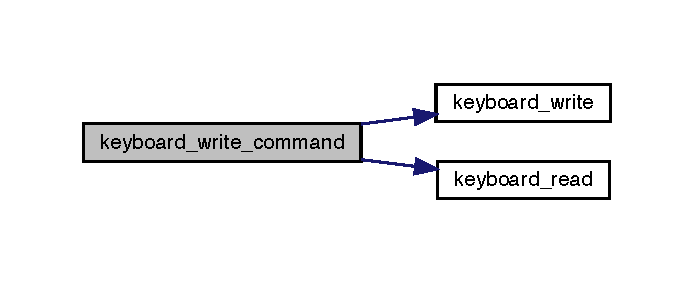
\includegraphics[width=333pt]{group__keyboard_ga279ddeca4cafee5084a0eec40e28d223_cgraph}
\end{center}
\end{figure}

\hypertarget{group__lmlib}{}\section{lmlib}
\label{group__lmlib}\index{lmlib@{lmlib}}
\subsection*{Classes}
\begin{DoxyCompactItemize}
\item 
struct \hyperlink{structmmap__t}{mmap\+\_\+t}
\end{DoxyCompactItemize}
\subsection*{Functions}
\begin{DoxyCompactItemize}
\item 
void $\ast$ \hyperlink{group__lmlib_ga00a9c17c01e794a6bfc80fc5c6ab1ed1}{lm\+\_\+init} (void)
\begin{DoxyCompactList}\small\item\em Initializes the low memory area, the region up to the 1 M\+Byte physical address, by mapping it on the process\textquotesingle{} physical memory address. \end{DoxyCompactList}\item 
void $\ast$ \hyperlink{group__lmlib_gae45d971ce2ffcf4dc2677eba033a92cd}{lm\+\_\+alloc} (unsigned long size, \hyperlink{structmmap__t}{mmap\+\_\+t} $\ast$map)
\begin{DoxyCompactList}\small\item\em Allocates a memory block in low memory area with the specified size. \end{DoxyCompactList}\item 
void \hyperlink{group__lmlib_ga73e89d9c297b7390021fb545513579c6}{lm\+\_\+free} (\hyperlink{structmmap__t}{mmap\+\_\+t} $\ast$map)
\begin{DoxyCompactList}\small\item\em Frees a memory block in the low memory area, previously allocated using \hyperlink{group__lmlib_gae45d971ce2ffcf4dc2677eba033a92cd}{lm\+\_\+alloc()} \end{DoxyCompactList}\end{DoxyCompactItemize}
\subsection*{Variables}
\begin{DoxyCompactItemize}
\item 
phys\+\_\+bytes \hyperlink{group__lmlib_gaa6ac1ee0e0fadea4a4f85b48c8359ae4}{mmap\+\_\+t\+::phys}
\begin{DoxyCompactList}\small\item\em physical address \end{DoxyCompactList}\item 
void $\ast$ \hyperlink{group__lmlib_ga4de93144fb3ffbceb9bd1f3009d6d98c}{mmap\+\_\+t\+::virtual}
\begin{DoxyCompactList}\small\item\em virtual address \end{DoxyCompactList}\item 
unsigned long \hyperlink{group__lmlib_gaf1cdc5384a402fddf33f400a5e1e5e45}{mmap\+\_\+t\+::size}
\begin{DoxyCompactList}\small\item\em size of memory region \end{DoxyCompactList}\end{DoxyCompactItemize}


\subsection{Detailed Description}
Functions related to low memory (first 1 MB of physical memory), required for B\+I\+OS 

\subsection{Function Documentation}
\hypertarget{group__lmlib_gae45d971ce2ffcf4dc2677eba033a92cd}{}\label{group__lmlib_gae45d971ce2ffcf4dc2677eba033a92cd} 
\index{lmlib@{lmlib}!lm\+\_\+alloc@{lm\+\_\+alloc}}
\index{lm\+\_\+alloc@{lm\+\_\+alloc}!lmlib@{lmlib}}
\subsubsection{\texorpdfstring{lm\+\_\+alloc()}{lm\_alloc()}}
{\footnotesize\ttfamily void$\ast$ lm\+\_\+alloc (\begin{DoxyParamCaption}\item[{unsigned long}]{size,  }\item[{\hyperlink{structmmap__t}{mmap\+\_\+t} $\ast$}]{map }\end{DoxyParamCaption})}



Allocates a memory block in low memory area with the specified size. 

Allocates a memory block in the region up to the 1 M\+Byte physical address with the input size. Initializes the input \hyperlink{structmmap__t}{mmap\+\_\+t} struct with the maping information, which can be read but must not be modified.


\begin{DoxyParams}{Parameters}
{\em size} & size of the memory block to allocate \\
\hline
{\em map} & pointer to \hyperlink{structmmap__t}{mmap\+\_\+t} data structure, which represents the memory map \\
\hline
\end{DoxyParams}
\begin{DoxyReturn}{Returns}
the virtual address of the memory block on success, N\+U\+LL otherwise 
\end{DoxyReturn}
\hypertarget{group__lmlib_ga73e89d9c297b7390021fb545513579c6}{}\label{group__lmlib_ga73e89d9c297b7390021fb545513579c6} 
\index{lmlib@{lmlib}!lm\+\_\+free@{lm\+\_\+free}}
\index{lm\+\_\+free@{lm\+\_\+free}!lmlib@{lmlib}}
\subsubsection{\texorpdfstring{lm\+\_\+free()}{lm\_free()}}
{\footnotesize\ttfamily void lm\+\_\+free (\begin{DoxyParamCaption}\item[{\hyperlink{structmmap__t}{mmap\+\_\+t} $\ast$}]{map }\end{DoxyParamCaption})}



Frees a memory block in the low memory area, previously allocated using \hyperlink{group__lmlib_gae45d971ce2ffcf4dc2677eba033a92cd}{lm\+\_\+alloc()} 

Frees a memory block in the region up to the 1 M\+Byte physical addess, previously allocated using \hyperlink{group__lmlib_gae45d971ce2ffcf4dc2677eba033a92cd}{lm\+\_\+alloc()}. Takes as input the address of the \hyperlink{structmmap__t}{mmap\+\_\+t} structure that was passed to \hyperlink{group__lmlib_gae45d971ce2ffcf4dc2677eba033a92cd}{lm\+\_\+alloc()}, and that must have not been modified since.


\begin{DoxyParams}{Parameters}
{\em map} & pointer to \hyperlink{structmmap__t}{mmap\+\_\+t} data structure of the block being freed \\
\hline
\end{DoxyParams}
\hypertarget{group__lmlib_ga00a9c17c01e794a6bfc80fc5c6ab1ed1}{}\label{group__lmlib_ga00a9c17c01e794a6bfc80fc5c6ab1ed1} 
\index{lmlib@{lmlib}!lm\+\_\+init@{lm\+\_\+init}}
\index{lm\+\_\+init@{lm\+\_\+init}!lmlib@{lmlib}}
\subsubsection{\texorpdfstring{lm\+\_\+init()}{lm\_init()}}
{\footnotesize\ttfamily void$\ast$ lm\+\_\+init (\begin{DoxyParamCaption}\item[{void}]{ }\end{DoxyParamCaption})}



Initializes the low memory area, the region up to the 1 M\+Byte physical address, by mapping it on the process\textquotesingle{} physical memory address. 

\begin{DoxyReturn}{Returns}
virtual address on which the first 1 MiB was mapped, N\+U\+LL upon failure 
\end{DoxyReturn}


\subsection{Variable Documentation}
\hypertarget{group__lmlib_gaa6ac1ee0e0fadea4a4f85b48c8359ae4}{}\label{group__lmlib_gaa6ac1ee0e0fadea4a4f85b48c8359ae4} 
\index{lmlib@{lmlib}!phys@{phys}}
\index{phys@{phys}!lmlib@{lmlib}}
\subsubsection{\texorpdfstring{phys}{phys}}
{\footnotesize\ttfamily phys\+\_\+bytes mmap\+\_\+t\+::phys}



physical address 

\hypertarget{group__lmlib_gaf1cdc5384a402fddf33f400a5e1e5e45}{}\label{group__lmlib_gaf1cdc5384a402fddf33f400a5e1e5e45} 
\index{lmlib@{lmlib}!size@{size}}
\index{size@{size}!lmlib@{lmlib}}
\subsubsection{\texorpdfstring{size}{size}}
{\footnotesize\ttfamily unsigned long mmap\+\_\+t\+::size}



size of memory region 

\hypertarget{group__lmlib_ga4de93144fb3ffbceb9bd1f3009d6d98c}{}\label{group__lmlib_ga4de93144fb3ffbceb9bd1f3009d6d98c} 
\index{lmlib@{lmlib}!virtual@{virtual}}
\index{virtual@{virtual}!lmlib@{lmlib}}
\subsubsection{\texorpdfstring{virtual}{virtual}}
{\footnotesize\ttfamily void$\ast$ mmap\+\_\+t\+::virtual}



virtual address 


\hypertarget{group___missile}{}\section{Missile}
\label{group___missile}\index{Missile@{Missile}}
\subsection*{Typedefs}
\begin{DoxyCompactItemize}
\item 
typedef struct \hyperlink{structmissile__t}{missile\+\_\+t} \hyperlink{group___missile_ga7ea98f7c879356e5dfa41934529d86e1}{Missile}
\item 
typedef struct \hyperlink{structexplosion__t}{explosion\+\_\+t} \hyperlink{group___missile_gab15157e0eccd9297f66644015d4966b1}{Explosion}
\end{DoxyCompactItemize}
\subsection*{Functions}
\begin{DoxyCompactItemize}
\item 
\hyperlink{group___missile_ga7ea98f7c879356e5dfa41934529d86e1}{Missile} $\ast$ \hyperlink{group___missile_ga6a34d606d98bc4ce9643a20ba65fd472}{new\+\_\+emissile} (const unsigned $\ast$bases\+\_\+pos, const unsigned $\ast$bases\+\_\+hp)
\begin{DoxyCompactList}\small\item\em Generates a new enemy missile. \end{DoxyCompactList}\item 
\hyperlink{group___missile_ga7ea98f7c879356e5dfa41934529d86e1}{Missile} $\ast$ \hyperlink{group___missile_ga163468dc0fdc7c61c009528ed5099753}{new\+\_\+fmissile} (const int $\ast$init\+\_\+pos, const int $\ast$mouse\+\_\+pos)
\begin{DoxyCompactList}\small\item\em Generates a new friendly missile. \end{DoxyCompactList}\item 
size\+\_\+t \hyperlink{group___missile_gad5e9a748d3bf909e91ceef47f63ee0d4}{missile\+\_\+get\+Size\+Of} ()
\begin{DoxyCompactList}\small\item\em Size of the space of memory occupied by a Missile T\+O\+DO\+: Recheck. \end{DoxyCompactList}\item 
int \hyperlink{group___missile_gabfb8e910eca430d5538a6d5b3ec8cb6e}{missile\+\_\+get\+PosX} (\hyperlink{group___missile_ga7ea98f7c879356e5dfa41934529d86e1}{Missile} $\ast$ptr)
\begin{DoxyCompactList}\small\item\em Gets the position in the horizontal axis of the Missile, on the screen. \end{DoxyCompactList}\item 
int \hyperlink{group___missile_gaef773d140afb584ac01d494d0f7c02e8}{missile\+\_\+get\+PosY} (\hyperlink{group___missile_ga7ea98f7c879356e5dfa41934529d86e1}{Missile} $\ast$ptr)
\begin{DoxyCompactList}\small\item\em Gets the position in the vertical axis of the Missile, on the screen. \end{DoxyCompactList}\item 
int \hyperlink{group___missile_ga6bcfcaf70f8810ab5f93275926fea9b8}{missile\+\_\+get\+InitX} (\hyperlink{group___missile_ga7ea98f7c879356e5dfa41934529d86e1}{Missile} $\ast$ptr)
\begin{DoxyCompactList}\small\item\em Gets the initial position in the horizontal axis of the Missile, on the screen. \end{DoxyCompactList}\item 
int \hyperlink{group___missile_ga6083be12aadde673a28d0a391391f96e}{missile\+\_\+get\+InitY} (\hyperlink{group___missile_ga7ea98f7c879356e5dfa41934529d86e1}{Missile} $\ast$ptr)
\begin{DoxyCompactList}\small\item\em Gets the initial position in the vertical axis of the Missile, on the screen. \end{DoxyCompactList}\item 
uint16\+\_\+t \hyperlink{group___missile_gafd665dec928dec0b42baf150444daa58}{missile\+\_\+get\+Color} (\hyperlink{group___missile_ga7ea98f7c879356e5dfa41934529d86e1}{Missile} $\ast$ptr)
\begin{DoxyCompactList}\small\item\em Gets the color of the Missile. \end{DoxyCompactList}\item 
int \hyperlink{group___missile_ga6d0e1c431aa7534db74504a9505a7b60}{missile\+\_\+update} (\hyperlink{group___missile_ga7ea98f7c879356e5dfa41934529d86e1}{Missile} $\ast$ptr)
\begin{DoxyCompactList}\small\item\em Updates the Missile, more specifically its position on the screen. \end{DoxyCompactList}\item 
int \hyperlink{group___missile_gae9eff55a2ebd486cc44daf149176e771}{missile\+\_\+is\+Friendly} (\hyperlink{group___missile_ga7ea98f7c879356e5dfa41934529d86e1}{Missile} $\ast$ptr)
\begin{DoxyCompactList}\small\item\em Checks if a Missile is friendly. \end{DoxyCompactList}\item 
\hyperlink{group___missile_gab15157e0eccd9297f66644015d4966b1}{Explosion} $\ast$ \hyperlink{group___missile_ga693cd51b6557695cb6593b56fbc89df8}{delete\+\_\+missile} (\hyperlink{group___missile_ga7ea98f7c879356e5dfa41934529d86e1}{Missile} $\ast$ptr)
\begin{DoxyCompactList}\small\item\em Destroys a missile, freeing all the resources used by it. \end{DoxyCompactList}\item 
\hyperlink{group___missile_gab15157e0eccd9297f66644015d4966b1}{Explosion} $\ast$ \hyperlink{group___missile_ga26a5cb6dc4144b31bb2005e4b587ff4f}{new\+\_\+explosion} (const int $\ast$position)
\begin{DoxyCompactList}\small\item\em Creates an explosion at a given position. \end{DoxyCompactList}\item 
int \hyperlink{group___missile_gabc0219cffe0a8c0060dabb7dfab4dbc3}{explosion\+\_\+update} (\hyperlink{group___missile_gab15157e0eccd9297f66644015d4966b1}{Explosion} $\ast$ptr)
\begin{DoxyCompactList}\small\item\em Updates the Explosion, more specifically the radius of the explosion its animation. \end{DoxyCompactList}\item 
\hyperlink{struct_bitmap}{Bitmap} $\ast$ \hyperlink{group___missile_ga1f8e365295b2facc195f17155bba6b71}{explosion\+\_\+get\+Bitmap} (\hyperlink{group___missile_gab15157e0eccd9297f66644015d4966b1}{Explosion} $\ast$ptr)
\begin{DoxyCompactList}\small\item\em Gets the current \hyperlink{struct_bitmap}{Bitmap} of the Explosion. \end{DoxyCompactList}\item 
int \hyperlink{group___missile_gaaa4dd8460fa2eeb803f0e62b0b693589}{explosion\+\_\+get\+PosX} (\hyperlink{group___missile_gab15157e0eccd9297f66644015d4966b1}{Explosion} $\ast$ptr)
\begin{DoxyCompactList}\small\item\em Gets the position in the horizontal axis of the Explosion, on the screen. \end{DoxyCompactList}\item 
int \hyperlink{group___missile_gab7f446e98be5f55752942865f5e10be4}{explosion\+\_\+get\+PosY} (\hyperlink{group___missile_gab15157e0eccd9297f66644015d4966b1}{Explosion} $\ast$ptr)
\begin{DoxyCompactList}\small\item\em Gets the position in the vertical axis of the Explosion, on the screen. \end{DoxyCompactList}\item 
size\+\_\+t \hyperlink{group___missile_ga41c747ea318363b16bce9e8bb8ea19ec}{explosion\+\_\+get\+Size\+Of} ()
\begin{DoxyCompactList}\small\item\em \char`\"{}get\char`\"{} method for retrieving sizeof(\+Explosion) \end{DoxyCompactList}\item 
void \hyperlink{group___missile_ga41c05f1f6d72a4c84b12d595b9ae8cbc}{delete\+\_\+explosion} (\hyperlink{group___missile_gab15157e0eccd9297f66644015d4966b1}{Explosion} $\ast$ptr)
\begin{DoxyCompactList}\small\item\em Destroys an Explosion, freeing all the resources used by it. \end{DoxyCompactList}\item 
int \hyperlink{group___missile_gab2d6dfae85e8db5dd6444161120f2fc1}{missile\+\_\+collided\+With\+Explosion} (\hyperlink{group___missile_ga7ea98f7c879356e5dfa41934529d86e1}{Missile} $\ast$ptr, \hyperlink{group___missile_gab15157e0eccd9297f66644015d4966b1}{Explosion} $\ast$e\+\_\+ptr)
\begin{DoxyCompactList}\small\item\em Check if a Missile collided with a certain Explosion. \end{DoxyCompactList}\item 
int \hyperlink{group___missile_gacc30474e7e5f9cf52f0b41dcc27aa231}{missile\+\_\+collided\+With\+Rect} (\hyperlink{group___missile_ga7ea98f7c879356e5dfa41934529d86e1}{Missile} $\ast$ptr, unsigned posX, unsigned posY, unsigned sizeX, unsigned sizeY)
\begin{DoxyCompactList}\small\item\em Check if a Missile collided with a Rectangle. \end{DoxyCompactList}\end{DoxyCompactItemize}


\subsection{Detailed Description}
Functions for manipulating both the Missiles and the Explosions 

\subsection{Typedef Documentation}
\hypertarget{group___missile_gab15157e0eccd9297f66644015d4966b1}{}\label{group___missile_gab15157e0eccd9297f66644015d4966b1} 
\index{Missile@{Missile}!Explosion@{Explosion}}
\index{Explosion@{Explosion}!Missile@{Missile}}
\subsubsection{\texorpdfstring{Explosion}{Explosion}}
{\footnotesize\ttfamily typedef struct \hyperlink{structexplosion__t}{explosion\+\_\+t} \hyperlink{group___missile_gab15157e0eccd9297f66644015d4966b1}{Explosion}}

\hypertarget{group___missile_ga7ea98f7c879356e5dfa41934529d86e1}{}\label{group___missile_ga7ea98f7c879356e5dfa41934529d86e1} 
\index{Missile@{Missile}!Missile@{Missile}}
\index{Missile@{Missile}!Missile@{Missile}}
\subsubsection{\texorpdfstring{Missile}{Missile}}
{\footnotesize\ttfamily typedef struct \hyperlink{structmissile__t}{missile\+\_\+t} \hyperlink{group___missile_ga7ea98f7c879356e5dfa41934529d86e1}{Missile}}



\subsection{Function Documentation}
\hypertarget{group___missile_ga41c05f1f6d72a4c84b12d595b9ae8cbc}{}\label{group___missile_ga41c05f1f6d72a4c84b12d595b9ae8cbc} 
\index{Missile@{Missile}!delete\+\_\+explosion@{delete\+\_\+explosion}}
\index{delete\+\_\+explosion@{delete\+\_\+explosion}!Missile@{Missile}}
\subsubsection{\texorpdfstring{delete\+\_\+explosion()}{delete\_explosion()}}
{\footnotesize\ttfamily void delete\+\_\+explosion (\begin{DoxyParamCaption}\item[{\hyperlink{group___missile_gab15157e0eccd9297f66644015d4966b1}{Explosion} $\ast$}]{ptr }\end{DoxyParamCaption})}



Destroys an Explosion, freeing all the resources used by it. 


\begin{DoxyParams}{Parameters}
{\em ptr} & Pointer to the Explosion in question \\
\hline
\end{DoxyParams}
\hypertarget{group___missile_ga693cd51b6557695cb6593b56fbc89df8}{}\label{group___missile_ga693cd51b6557695cb6593b56fbc89df8} 
\index{Missile@{Missile}!delete\+\_\+missile@{delete\+\_\+missile}}
\index{delete\+\_\+missile@{delete\+\_\+missile}!Missile@{Missile}}
\subsubsection{\texorpdfstring{delete\+\_\+missile()}{delete\_missile()}}
{\footnotesize\ttfamily \hyperlink{group___missile_gab15157e0eccd9297f66644015d4966b1}{Explosion}$\ast$ delete\+\_\+missile (\begin{DoxyParamCaption}\item[{\hyperlink{group___missile_ga7ea98f7c879356e5dfa41934529d86e1}{Missile} $\ast$}]{ptr }\end{DoxyParamCaption})}



Destroys a missile, freeing all the resources used by it. 


\begin{DoxyParams}{Parameters}
{\em ptr} & Pointer to the Missile in question\\
\hline
\end{DoxyParams}
\begin{DoxyReturn}{Returns}
Pointer to an explosion that will start at the last position of the missile 
\end{DoxyReturn}
Here is the call graph for this function\+:\nopagebreak
\begin{figure}[H]
\begin{center}
\leavevmode
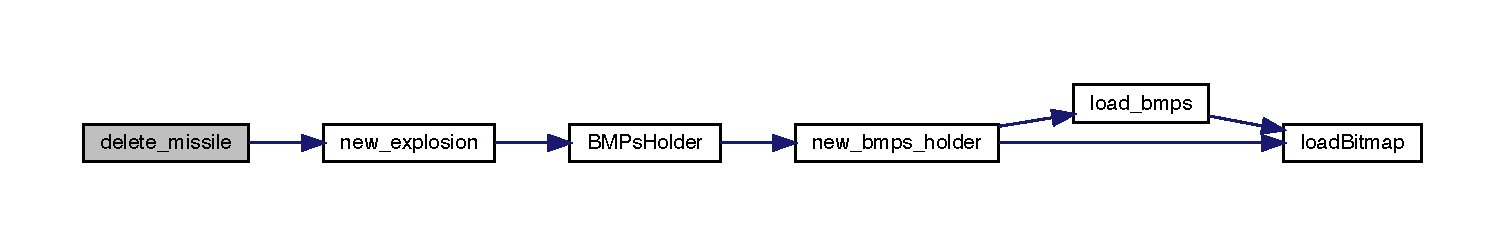
\includegraphics[width=350pt]{group___missile_ga693cd51b6557695cb6593b56fbc89df8_cgraph}
\end{center}
\end{figure}
\hypertarget{group___missile_ga1f8e365295b2facc195f17155bba6b71}{}\label{group___missile_ga1f8e365295b2facc195f17155bba6b71} 
\index{Missile@{Missile}!explosion\+\_\+get\+Bitmap@{explosion\+\_\+get\+Bitmap}}
\index{explosion\+\_\+get\+Bitmap@{explosion\+\_\+get\+Bitmap}!Missile@{Missile}}
\subsubsection{\texorpdfstring{explosion\+\_\+get\+Bitmap()}{explosion\_getBitmap()}}
{\footnotesize\ttfamily \hyperlink{struct_bitmap}{Bitmap}$\ast$ explosion\+\_\+get\+Bitmap (\begin{DoxyParamCaption}\item[{\hyperlink{group___missile_gab15157e0eccd9297f66644015d4966b1}{Explosion} $\ast$}]{ptr }\end{DoxyParamCaption})}



Gets the current \hyperlink{struct_bitmap}{Bitmap} of the Explosion. 


\begin{DoxyParams}{Parameters}
{\em ptr} & Pointer to the Explosion in question\\
\hline
\end{DoxyParams}
\begin{DoxyReturn}{Returns}
Return the current \hyperlink{struct_bitmap}{Bitmap} of the Explosion 
\end{DoxyReturn}
\hypertarget{group___missile_gaaa4dd8460fa2eeb803f0e62b0b693589}{}\label{group___missile_gaaa4dd8460fa2eeb803f0e62b0b693589} 
\index{Missile@{Missile}!explosion\+\_\+get\+PosX@{explosion\+\_\+get\+PosX}}
\index{explosion\+\_\+get\+PosX@{explosion\+\_\+get\+PosX}!Missile@{Missile}}
\subsubsection{\texorpdfstring{explosion\+\_\+get\+Pos\+X()}{explosion\_getPosX()}}
{\footnotesize\ttfamily int explosion\+\_\+get\+PosX (\begin{DoxyParamCaption}\item[{\hyperlink{group___missile_gab15157e0eccd9297f66644015d4966b1}{Explosion} $\ast$}]{ptr }\end{DoxyParamCaption})}



Gets the position in the horizontal axis of the Explosion, on the screen. 


\begin{DoxyParams}{Parameters}
{\em ptr} & Pointer to the Explosion in question\\
\hline
\end{DoxyParams}
\begin{DoxyReturn}{Returns}
position in the horizontal axis of the Explosion, on the screen 
\end{DoxyReturn}
\hypertarget{group___missile_gab7f446e98be5f55752942865f5e10be4}{}\label{group___missile_gab7f446e98be5f55752942865f5e10be4} 
\index{Missile@{Missile}!explosion\+\_\+get\+PosY@{explosion\+\_\+get\+PosY}}
\index{explosion\+\_\+get\+PosY@{explosion\+\_\+get\+PosY}!Missile@{Missile}}
\subsubsection{\texorpdfstring{explosion\+\_\+get\+Pos\+Y()}{explosion\_getPosY()}}
{\footnotesize\ttfamily int explosion\+\_\+get\+PosY (\begin{DoxyParamCaption}\item[{\hyperlink{group___missile_gab15157e0eccd9297f66644015d4966b1}{Explosion} $\ast$}]{ptr }\end{DoxyParamCaption})}



Gets the position in the vertical axis of the Explosion, on the screen. 


\begin{DoxyParams}{Parameters}
{\em ptr} & Pointer to the Explosion in question\\
\hline
\end{DoxyParams}
\begin{DoxyReturn}{Returns}
position in the vertical axis of the Explosion, on the screen 
\end{DoxyReturn}
\hypertarget{group___missile_ga41c747ea318363b16bce9e8bb8ea19ec}{}\label{group___missile_ga41c747ea318363b16bce9e8bb8ea19ec} 
\index{Missile@{Missile}!explosion\+\_\+get\+Size\+Of@{explosion\+\_\+get\+Size\+Of}}
\index{explosion\+\_\+get\+Size\+Of@{explosion\+\_\+get\+Size\+Of}!Missile@{Missile}}
\subsubsection{\texorpdfstring{explosion\+\_\+get\+Size\+Of()}{explosion\_getSizeOf()}}
{\footnotesize\ttfamily size\+\_\+t explosion\+\_\+get\+Size\+Of (\begin{DoxyParamCaption}{ }\end{DoxyParamCaption})}



\char`\"{}get\char`\"{} method for retrieving sizeof(\+Explosion) 

\begin{DoxyReturn}{Returns}
Size of the space of memory occupied by an object of type Explosion 
\end{DoxyReturn}
\hypertarget{group___missile_gabc0219cffe0a8c0060dabb7dfab4dbc3}{}\label{group___missile_gabc0219cffe0a8c0060dabb7dfab4dbc3} 
\index{Missile@{Missile}!explosion\+\_\+update@{explosion\+\_\+update}}
\index{explosion\+\_\+update@{explosion\+\_\+update}!Missile@{Missile}}
\subsubsection{\texorpdfstring{explosion\+\_\+update()}{explosion\_update()}}
{\footnotesize\ttfamily int explosion\+\_\+update (\begin{DoxyParamCaption}\item[{\hyperlink{group___missile_gab15157e0eccd9297f66644015d4966b1}{Explosion} $\ast$}]{ptr }\end{DoxyParamCaption})}



Updates the Explosion, more specifically the radius of the explosion its animation. 


\begin{DoxyParams}{Parameters}
{\em ptr} & Pointer to the Explosion in question\\
\hline
\end{DoxyParams}
\begin{DoxyReturn}{Returns}
Return 1 if explosion has ended, 0 otherwise 
\end{DoxyReturn}
\hypertarget{group___missile_gab2d6dfae85e8db5dd6444161120f2fc1}{}\label{group___missile_gab2d6dfae85e8db5dd6444161120f2fc1} 
\index{Missile@{Missile}!missile\+\_\+collided\+With\+Explosion@{missile\+\_\+collided\+With\+Explosion}}
\index{missile\+\_\+collided\+With\+Explosion@{missile\+\_\+collided\+With\+Explosion}!Missile@{Missile}}
\subsubsection{\texorpdfstring{missile\+\_\+collided\+With\+Explosion()}{missile\_collidedWithExplosion()}}
{\footnotesize\ttfamily int missile\+\_\+collided\+With\+Explosion (\begin{DoxyParamCaption}\item[{\hyperlink{group___missile_ga7ea98f7c879356e5dfa41934529d86e1}{Missile} $\ast$}]{ptr,  }\item[{\hyperlink{group___missile_gab15157e0eccd9297f66644015d4966b1}{Explosion} $\ast$}]{e\+\_\+ptr }\end{DoxyParamCaption})}



Check if a Missile collided with a certain Explosion. 


\begin{DoxyParams}{Parameters}
{\em ptr} & Pointer to the Missile in question \\
\hline
{\em e\+\_\+ptr} & Pointer to the Explosion in question\\
\hline
\end{DoxyParams}
\begin{DoxyReturn}{Returns}
Return 1 if Collision happened, 0 otherwise 
\end{DoxyReturn}
\hypertarget{group___missile_gacc30474e7e5f9cf52f0b41dcc27aa231}{}\label{group___missile_gacc30474e7e5f9cf52f0b41dcc27aa231} 
\index{Missile@{Missile}!missile\+\_\+collided\+With\+Rect@{missile\+\_\+collided\+With\+Rect}}
\index{missile\+\_\+collided\+With\+Rect@{missile\+\_\+collided\+With\+Rect}!Missile@{Missile}}
\subsubsection{\texorpdfstring{missile\+\_\+collided\+With\+Rect()}{missile\_collidedWithRect()}}
{\footnotesize\ttfamily int missile\+\_\+collided\+With\+Rect (\begin{DoxyParamCaption}\item[{\hyperlink{group___missile_ga7ea98f7c879356e5dfa41934529d86e1}{Missile} $\ast$}]{ptr,  }\item[{unsigned}]{posX,  }\item[{unsigned}]{posY,  }\item[{unsigned}]{sizeX,  }\item[{unsigned}]{sizeY }\end{DoxyParamCaption})}



Check if a Missile collided with a Rectangle. 


\begin{DoxyParams}{Parameters}
{\em ptr} & Pointer to the Missile in question \\
\hline
{\em posX} & Lower left position of the rectangle in the horizontal axis \\
\hline
{\em posY} & Lower left position of the rectangle in the vertical axis \\
\hline
{\em sizeX} & Width of the rectangle \\
\hline
{\em sizeY} & Height of the rectangle\\
\hline
\end{DoxyParams}
\begin{DoxyReturn}{Returns}
Return 1 if Collision happened, 0 otherwise 
\end{DoxyReturn}
\hypertarget{group___missile_gafd665dec928dec0b42baf150444daa58}{}\label{group___missile_gafd665dec928dec0b42baf150444daa58} 
\index{Missile@{Missile}!missile\+\_\+get\+Color@{missile\+\_\+get\+Color}}
\index{missile\+\_\+get\+Color@{missile\+\_\+get\+Color}!Missile@{Missile}}
\subsubsection{\texorpdfstring{missile\+\_\+get\+Color()}{missile\_getColor()}}
{\footnotesize\ttfamily uint16\+\_\+t missile\+\_\+get\+Color (\begin{DoxyParamCaption}\item[{\hyperlink{group___missile_ga7ea98f7c879356e5dfa41934529d86e1}{Missile} $\ast$}]{ptr }\end{DoxyParamCaption})}



Gets the color of the Missile. 


\begin{DoxyParams}{Parameters}
{\em ptr} & Pointer to the Missile in question\\
\hline
\end{DoxyParams}
\begin{DoxyReturn}{Returns}
Color of the Missile 
\end{DoxyReturn}
\hypertarget{group___missile_ga6bcfcaf70f8810ab5f93275926fea9b8}{}\label{group___missile_ga6bcfcaf70f8810ab5f93275926fea9b8} 
\index{Missile@{Missile}!missile\+\_\+get\+InitX@{missile\+\_\+get\+InitX}}
\index{missile\+\_\+get\+InitX@{missile\+\_\+get\+InitX}!Missile@{Missile}}
\subsubsection{\texorpdfstring{missile\+\_\+get\+Init\+X()}{missile\_getInitX()}}
{\footnotesize\ttfamily int missile\+\_\+get\+InitX (\begin{DoxyParamCaption}\item[{\hyperlink{group___missile_ga7ea98f7c879356e5dfa41934529d86e1}{Missile} $\ast$}]{ptr }\end{DoxyParamCaption})}



Gets the initial position in the horizontal axis of the Missile, on the screen. 


\begin{DoxyParams}{Parameters}
{\em ptr} & Pointer to the Missile in question\\
\hline
\end{DoxyParams}
\begin{DoxyReturn}{Returns}
intial position in the horizontal axis of the Missile, on the screen 
\end{DoxyReturn}
\hypertarget{group___missile_ga6083be12aadde673a28d0a391391f96e}{}\label{group___missile_ga6083be12aadde673a28d0a391391f96e} 
\index{Missile@{Missile}!missile\+\_\+get\+InitY@{missile\+\_\+get\+InitY}}
\index{missile\+\_\+get\+InitY@{missile\+\_\+get\+InitY}!Missile@{Missile}}
\subsubsection{\texorpdfstring{missile\+\_\+get\+Init\+Y()}{missile\_getInitY()}}
{\footnotesize\ttfamily int missile\+\_\+get\+InitY (\begin{DoxyParamCaption}\item[{\hyperlink{group___missile_ga7ea98f7c879356e5dfa41934529d86e1}{Missile} $\ast$}]{ptr }\end{DoxyParamCaption})}



Gets the initial position in the vertical axis of the Missile, on the screen. 


\begin{DoxyParams}{Parameters}
{\em ptr} & Pointer to the Missile in question\\
\hline
\end{DoxyParams}
\begin{DoxyReturn}{Returns}
intial position in the vertical axis of the Missile, on the screen 
\end{DoxyReturn}
\hypertarget{group___missile_gabfb8e910eca430d5538a6d5b3ec8cb6e}{}\label{group___missile_gabfb8e910eca430d5538a6d5b3ec8cb6e} 
\index{Missile@{Missile}!missile\+\_\+get\+PosX@{missile\+\_\+get\+PosX}}
\index{missile\+\_\+get\+PosX@{missile\+\_\+get\+PosX}!Missile@{Missile}}
\subsubsection{\texorpdfstring{missile\+\_\+get\+Pos\+X()}{missile\_getPosX()}}
{\footnotesize\ttfamily int missile\+\_\+get\+PosX (\begin{DoxyParamCaption}\item[{\hyperlink{group___missile_ga7ea98f7c879356e5dfa41934529d86e1}{Missile} $\ast$}]{ptr }\end{DoxyParamCaption})}



Gets the position in the horizontal axis of the Missile, on the screen. 


\begin{DoxyParams}{Parameters}
{\em ptr} & Pointer to the Missile in question\\
\hline
\end{DoxyParams}
\begin{DoxyReturn}{Returns}
position in the horizontal axis of the Missile, on the screen 
\end{DoxyReturn}
\hypertarget{group___missile_gaef773d140afb584ac01d494d0f7c02e8}{}\label{group___missile_gaef773d140afb584ac01d494d0f7c02e8} 
\index{Missile@{Missile}!missile\+\_\+get\+PosY@{missile\+\_\+get\+PosY}}
\index{missile\+\_\+get\+PosY@{missile\+\_\+get\+PosY}!Missile@{Missile}}
\subsubsection{\texorpdfstring{missile\+\_\+get\+Pos\+Y()}{missile\_getPosY()}}
{\footnotesize\ttfamily int missile\+\_\+get\+PosY (\begin{DoxyParamCaption}\item[{\hyperlink{group___missile_ga7ea98f7c879356e5dfa41934529d86e1}{Missile} $\ast$}]{ptr }\end{DoxyParamCaption})}



Gets the position in the vertical axis of the Missile, on the screen. 


\begin{DoxyParams}{Parameters}
{\em ptr} & Pointer to the Missile in question\\
\hline
\end{DoxyParams}
\begin{DoxyReturn}{Returns}
position in the vertical axis of the Missile, on the screen 
\end{DoxyReturn}
\hypertarget{group___missile_gad5e9a748d3bf909e91ceef47f63ee0d4}{}\label{group___missile_gad5e9a748d3bf909e91ceef47f63ee0d4} 
\index{Missile@{Missile}!missile\+\_\+get\+Size\+Of@{missile\+\_\+get\+Size\+Of}}
\index{missile\+\_\+get\+Size\+Of@{missile\+\_\+get\+Size\+Of}!Missile@{Missile}}
\subsubsection{\texorpdfstring{missile\+\_\+get\+Size\+Of()}{missile\_getSizeOf()}}
{\footnotesize\ttfamily size\+\_\+t missile\+\_\+get\+Size\+Of (\begin{DoxyParamCaption}{ }\end{DoxyParamCaption})}



Size of the space of memory occupied by a Missile T\+O\+DO\+: Recheck. 

\begin{DoxyReturn}{Returns}
Size of the space of memory occupied by a Missile 
\end{DoxyReturn}
\hypertarget{group___missile_gae9eff55a2ebd486cc44daf149176e771}{}\label{group___missile_gae9eff55a2ebd486cc44daf149176e771} 
\index{Missile@{Missile}!missile\+\_\+is\+Friendly@{missile\+\_\+is\+Friendly}}
\index{missile\+\_\+is\+Friendly@{missile\+\_\+is\+Friendly}!Missile@{Missile}}
\subsubsection{\texorpdfstring{missile\+\_\+is\+Friendly()}{missile\_isFriendly()}}
{\footnotesize\ttfamily int missile\+\_\+is\+Friendly (\begin{DoxyParamCaption}\item[{\hyperlink{group___missile_ga7ea98f7c879356e5dfa41934529d86e1}{Missile} $\ast$}]{ptr }\end{DoxyParamCaption})}



Checks if a Missile is friendly. 


\begin{DoxyParams}{Parameters}
{\em ptr} & Pointer to the Missile in question\\
\hline
\end{DoxyParams}
\begin{DoxyReturn}{Returns}
Return 1 upon success, 0 otherwise 
\end{DoxyReturn}
\hypertarget{group___missile_ga6d0e1c431aa7534db74504a9505a7b60}{}\label{group___missile_ga6d0e1c431aa7534db74504a9505a7b60} 
\index{Missile@{Missile}!missile\+\_\+update@{missile\+\_\+update}}
\index{missile\+\_\+update@{missile\+\_\+update}!Missile@{Missile}}
\subsubsection{\texorpdfstring{missile\+\_\+update()}{missile\_update()}}
{\footnotesize\ttfamily int missile\+\_\+update (\begin{DoxyParamCaption}\item[{\hyperlink{group___missile_ga7ea98f7c879356e5dfa41934529d86e1}{Missile} $\ast$}]{ptr }\end{DoxyParamCaption})}



Updates the Missile, more specifically its position on the screen. 


\begin{DoxyParams}{Parameters}
{\em ptr} & Pointer to the Missile in question\\
\hline
\end{DoxyParams}
\begin{DoxyReturn}{Returns}
In case a friendly missile has reached it\textquotesingle{}s end position returns 1, otherwise returns 0; 
\end{DoxyReturn}
Here is the call graph for this function\+:\nopagebreak
\begin{figure}[H]
\begin{center}
\leavevmode
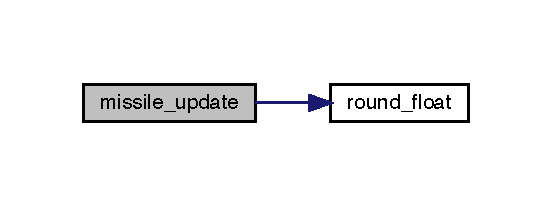
\includegraphics[width=265pt]{group___missile_ga6d0e1c431aa7534db74504a9505a7b60_cgraph}
\end{center}
\end{figure}
\hypertarget{group___missile_ga6a34d606d98bc4ce9643a20ba65fd472}{}\label{group___missile_ga6a34d606d98bc4ce9643a20ba65fd472} 
\index{Missile@{Missile}!new\+\_\+emissile@{new\+\_\+emissile}}
\index{new\+\_\+emissile@{new\+\_\+emissile}!Missile@{Missile}}
\subsubsection{\texorpdfstring{new\+\_\+emissile()}{new\_emissile()}}
{\footnotesize\ttfamily \hyperlink{group___missile_ga7ea98f7c879356e5dfa41934529d86e1}{Missile}$\ast$ new\+\_\+emissile (\begin{DoxyParamCaption}\item[{const unsigned $\ast$}]{bases\+\_\+pos,  }\item[{const unsigned $\ast$}]{bases\+\_\+hp }\end{DoxyParamCaption})}



Generates a new enemy missile. 


\begin{DoxyParams}{Parameters}
{\em bases\+\_\+pos} & Array containing the bases\textquotesingle{} positions, so the missile can randomly target one \\
\hline
{\em bases\+\_\+hp} & Array containing the bases\textquotesingle{} Health Points, to avoid dead bases\\
\hline
\end{DoxyParams}
\begin{DoxyReturn}{Returns}
Pointer to the the newly created enemy missile
\end{DoxyReturn}
Constructor for Enemy Missile Here is the call graph for this function\+:\nopagebreak
\begin{figure}[H]
\begin{center}
\leavevmode
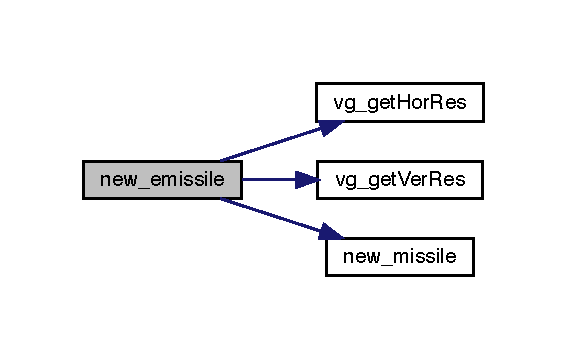
\includegraphics[width=272pt]{group___missile_ga6a34d606d98bc4ce9643a20ba65fd472_cgraph}
\end{center}
\end{figure}
\hypertarget{group___missile_ga26a5cb6dc4144b31bb2005e4b587ff4f}{}\label{group___missile_ga26a5cb6dc4144b31bb2005e4b587ff4f} 
\index{Missile@{Missile}!new\+\_\+explosion@{new\+\_\+explosion}}
\index{new\+\_\+explosion@{new\+\_\+explosion}!Missile@{Missile}}
\subsubsection{\texorpdfstring{new\+\_\+explosion()}{new\_explosion()}}
{\footnotesize\ttfamily \hyperlink{group___missile_gab15157e0eccd9297f66644015d4966b1}{Explosion}$\ast$ new\+\_\+explosion (\begin{DoxyParamCaption}\item[{const int $\ast$}]{position }\end{DoxyParamCaption})}



Creates an explosion at a given position. 


\begin{DoxyParams}{Parameters}
{\em position} & Array containing the position where the explosion starts (x,y)\\
\hline
\end{DoxyParams}
\begin{DoxyReturn}{Returns}
Pointer to the newly created explosion
\end{DoxyReturn}
Methods for Explosion Here is the call graph for this function\+:\nopagebreak
\begin{figure}[H]
\begin{center}
\leavevmode
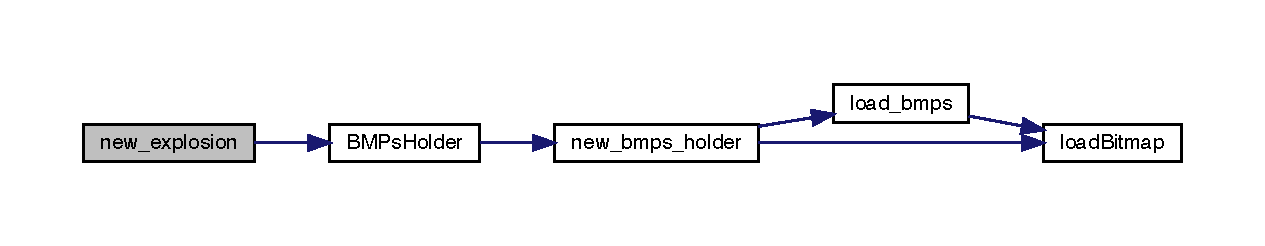
\includegraphics[width=350pt]{group___missile_ga26a5cb6dc4144b31bb2005e4b587ff4f_cgraph}
\end{center}
\end{figure}
\hypertarget{group___missile_ga163468dc0fdc7c61c009528ed5099753}{}\label{group___missile_ga163468dc0fdc7c61c009528ed5099753} 
\index{Missile@{Missile}!new\+\_\+fmissile@{new\+\_\+fmissile}}
\index{new\+\_\+fmissile@{new\+\_\+fmissile}!Missile@{Missile}}
\subsubsection{\texorpdfstring{new\+\_\+fmissile()}{new\_fmissile()}}
{\footnotesize\ttfamily \hyperlink{group___missile_ga7ea98f7c879356e5dfa41934529d86e1}{Missile}$\ast$ new\+\_\+fmissile (\begin{DoxyParamCaption}\item[{const int $\ast$}]{init\+\_\+pos,  }\item[{const int $\ast$}]{mouse\+\_\+pos }\end{DoxyParamCaption})}



Generates a new friendly missile. 


\begin{DoxyParams}{Parameters}
{\em init\+\_\+pos} & Array containing the initial position of the missile (x,y), associated to the cannon that fired it. \\
\hline
{\em mouse\+\_\+pos} & Array containing the mouse position where the friendly missile will explode\\
\hline
\end{DoxyParams}
\begin{DoxyReturn}{Returns}
Pointer to the newly created friendly missile Generates a new friendly missile
\end{DoxyReturn}

\begin{DoxyParams}{Parameters}
{\em init\+\_\+pos} & Array containing the initial position of the missile (x,y), associated to the cannon that fired it. \\
\hline
{\em mouse\+\_\+pos} & Array containing the mouse position where the friendly missile will explode\\
\hline
\end{DoxyParams}
\begin{DoxyReturn}{Returns}
Pointer to the newly created friendly missile
\end{DoxyReturn}
Constructor for Friendly Missile Here is the call graph for this function\+:\nopagebreak
\begin{figure}[H]
\begin{center}
\leavevmode
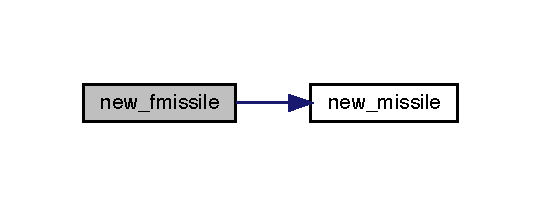
\includegraphics[width=260pt]{group___missile_ga163468dc0fdc7c61c009528ed5099753_cgraph}
\end{center}
\end{figure}

\hypertarget{group__mouse}{}\section{mouse}
\label{group__mouse}\index{mouse@{mouse}}
\subsection*{Functions}
\begin{DoxyCompactItemize}
\item 
int \hyperlink{group__mouse_gaf67a039319066d9e7dcdcc90e3a48840}{int\+\_\+value} (unsigned char delta\+\_\+var, int sign)
\begin{DoxyCompactList}\small\item\em Function to get the signed value of an unsigned value. \end{DoxyCompactList}\item 
int \hyperlink{group__mouse_gad26aa3828c4a6d900e654de8e4e68e83}{mouse\+\_\+write\+\_\+cmd} (char cmd)
\begin{DoxyCompactList}\small\item\em Writes a command in the mouse input buffer. \end{DoxyCompactList}\item 
int \hyperlink{group__mouse_ga51e6ee02a5c0a7e618abde7250cd0841}{mouse\+\_\+subscribe\+\_\+int} (void)
\begin{DoxyCompactList}\small\item\em Subscribes and enables Mouse interrupts. \end{DoxyCompactList}\item 
int \hyperlink{group__mouse_ga7614d1f22092d37078f6a3da58f7c957}{mouse\+\_\+unsubscribe\+\_\+int} (void)
\begin{DoxyCompactList}\small\item\em Unsubscribes Mouse interrupts. \end{DoxyCompactList}\item 
int \hyperlink{group__mouse_gacf07c98dc574238b3da9388c3dd1042a}{mouse\+\_\+synchronize} (void)
\begin{DoxyCompactList}\small\item\em Synchronizes the mouse. \end{DoxyCompactList}\item 
int \hyperlink{group__mouse_gaaff93ce65c5bddd94904122f0e336233}{mouse\+\_\+read} (void)
\begin{DoxyCompactList}\small\item\em Reads data from the mouse output buffer. \end{DoxyCompactList}\item 
int \hyperlink{group__mouse_gab5168a5f260c8e28f0f75db8a35cdb98}{mouse\+\_\+handler} (unsigned char $\ast$packet, unsigned short $\ast$counter)
\begin{DoxyCompactList}\small\item\em Mouse Interrupt Handler. \end{DoxyCompactList}\end{DoxyCompactItemize}


\subsection{Detailed Description}
Functions for using the i8042 K\+B\+C/\+K\+BD 

\subsection{Function Documentation}
\hypertarget{group__mouse_gaf67a039319066d9e7dcdcc90e3a48840}{}\label{group__mouse_gaf67a039319066d9e7dcdcc90e3a48840} 
\index{mouse@{mouse}!int\+\_\+value@{int\+\_\+value}}
\index{int\+\_\+value@{int\+\_\+value}!mouse@{mouse}}
\subsubsection{\texorpdfstring{int\+\_\+value()}{int\_value()}}
{\footnotesize\ttfamily int int\+\_\+value (\begin{DoxyParamCaption}\item[{unsigned char}]{delta\+\_\+var,  }\item[{int}]{sign }\end{DoxyParamCaption})}



Function to get the signed value of an unsigned value. 


\begin{DoxyParams}{Parameters}
{\em delta\+\_\+var} & Unsigned value that will be processed \\
\hline
{\em sign} & Sign of the unsigned value\\
\hline
\end{DoxyParams}
\begin{DoxyReturn}{Returns}
Return the signed value 
\end{DoxyReturn}
\hypertarget{group__mouse_gab5168a5f260c8e28f0f75db8a35cdb98}{}\label{group__mouse_gab5168a5f260c8e28f0f75db8a35cdb98} 
\index{mouse@{mouse}!mouse\+\_\+handler@{mouse\+\_\+handler}}
\index{mouse\+\_\+handler@{mouse\+\_\+handler}!mouse@{mouse}}
\subsubsection{\texorpdfstring{mouse\+\_\+handler()}{mouse\_handler()}}
{\footnotesize\ttfamily int mouse\+\_\+handler (\begin{DoxyParamCaption}\item[{unsigned char $\ast$}]{packet,  }\item[{unsigned short $\ast$}]{counter }\end{DoxyParamCaption})}



Mouse Interrupt Handler. 

Fetches Mouse output and prints packets in a human friendly way


\begin{DoxyParams}{Parameters}
{\em packet} & pointer to packet that shall be processed \\
\hline
{\em counter} & pointer to counter that controls the packet count of bytes\\
\hline
\end{DoxyParams}
\begin{DoxyReturn}{Returns}
Return 0 upon success and non-\/zero otherwise 
\end{DoxyReturn}
Here is the call graph for this function\+:\nopagebreak
\begin{figure}[H]
\begin{center}
\leavevmode
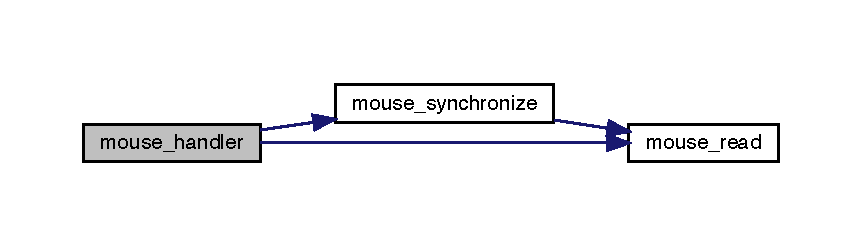
\includegraphics[width=350pt]{group__mouse_gab5168a5f260c8e28f0f75db8a35cdb98_cgraph}
\end{center}
\end{figure}
\hypertarget{group__mouse_gaaff93ce65c5bddd94904122f0e336233}{}\label{group__mouse_gaaff93ce65c5bddd94904122f0e336233} 
\index{mouse@{mouse}!mouse\+\_\+read@{mouse\+\_\+read}}
\index{mouse\+\_\+read@{mouse\+\_\+read}!mouse@{mouse}}
\subsubsection{\texorpdfstring{mouse\+\_\+read()}{mouse\_read()}}
{\footnotesize\ttfamily int mouse\+\_\+read (\begin{DoxyParamCaption}\item[{void}]{ }\end{DoxyParamCaption})}



Reads data from the mouse output buffer. 

\begin{DoxyReturn}{Returns}
Return value read upon sucess and -\/1 otherwise 
\end{DoxyReturn}
\hypertarget{group__mouse_ga51e6ee02a5c0a7e618abde7250cd0841}{}\label{group__mouse_ga51e6ee02a5c0a7e618abde7250cd0841} 
\index{mouse@{mouse}!mouse\+\_\+subscribe\+\_\+int@{mouse\+\_\+subscribe\+\_\+int}}
\index{mouse\+\_\+subscribe\+\_\+int@{mouse\+\_\+subscribe\+\_\+int}!mouse@{mouse}}
\subsubsection{\texorpdfstring{mouse\+\_\+subscribe\+\_\+int()}{mouse\_subscribe\_int()}}
{\footnotesize\ttfamily int mouse\+\_\+subscribe\+\_\+int (\begin{DoxyParamCaption}\item[{void}]{ }\end{DoxyParamCaption})}



Subscribes and enables Mouse interrupts. 

\begin{DoxyReturn}{Returns}
Returns bit order in interrupt mask; negative value on failure 
\end{DoxyReturn}
Here is the call graph for this function\+:\nopagebreak
\begin{figure}[H]
\begin{center}
\leavevmode
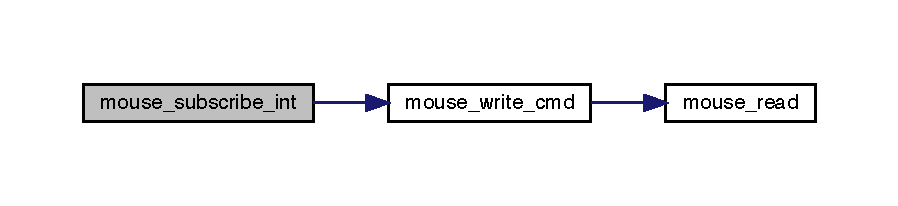
\includegraphics[width=350pt]{group__mouse_ga51e6ee02a5c0a7e618abde7250cd0841_cgraph}
\end{center}
\end{figure}
\hypertarget{group__mouse_gacf07c98dc574238b3da9388c3dd1042a}{}\label{group__mouse_gacf07c98dc574238b3da9388c3dd1042a} 
\index{mouse@{mouse}!mouse\+\_\+synchronize@{mouse\+\_\+synchronize}}
\index{mouse\+\_\+synchronize@{mouse\+\_\+synchronize}!mouse@{mouse}}
\subsubsection{\texorpdfstring{mouse\+\_\+synchronize()}{mouse\_synchronize()}}
{\footnotesize\ttfamily int mouse\+\_\+synchronize (\begin{DoxyParamCaption}\item[{void}]{ }\end{DoxyParamCaption})}



Synchronizes the mouse. 

\begin{DoxyReturn}{Returns}
Return byte1 upon sucess and -\/1 otherwise 
\end{DoxyReturn}
Here is the call graph for this function\+:\nopagebreak
\begin{figure}[H]
\begin{center}
\leavevmode
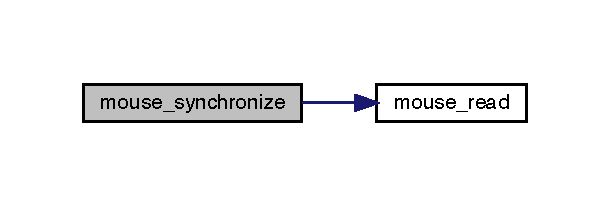
\includegraphics[width=293pt]{group__mouse_gacf07c98dc574238b3da9388c3dd1042a_cgraph}
\end{center}
\end{figure}
\hypertarget{group__mouse_ga7614d1f22092d37078f6a3da58f7c957}{}\label{group__mouse_ga7614d1f22092d37078f6a3da58f7c957} 
\index{mouse@{mouse}!mouse\+\_\+unsubscribe\+\_\+int@{mouse\+\_\+unsubscribe\+\_\+int}}
\index{mouse\+\_\+unsubscribe\+\_\+int@{mouse\+\_\+unsubscribe\+\_\+int}!mouse@{mouse}}
\subsubsection{\texorpdfstring{mouse\+\_\+unsubscribe\+\_\+int()}{mouse\_unsubscribe\_int()}}
{\footnotesize\ttfamily int mouse\+\_\+unsubscribe\+\_\+int (\begin{DoxyParamCaption}\item[{void}]{ }\end{DoxyParamCaption})}



Unsubscribes Mouse interrupts. 

\begin{DoxyReturn}{Returns}
Return 0 upon success and non-\/zero otherwise 
\end{DoxyReturn}
\hypertarget{group__mouse_gad26aa3828c4a6d900e654de8e4e68e83}{}\label{group__mouse_gad26aa3828c4a6d900e654de8e4e68e83} 
\index{mouse@{mouse}!mouse\+\_\+write\+\_\+cmd@{mouse\+\_\+write\+\_\+cmd}}
\index{mouse\+\_\+write\+\_\+cmd@{mouse\+\_\+write\+\_\+cmd}!mouse@{mouse}}
\subsubsection{\texorpdfstring{mouse\+\_\+write\+\_\+cmd()}{mouse\_write\_cmd()}}
{\footnotesize\ttfamily int mouse\+\_\+write\+\_\+cmd (\begin{DoxyParamCaption}\item[{char}]{cmd }\end{DoxyParamCaption})}



Writes a command in the mouse input buffer. 


\begin{DoxyParams}{Parameters}
{\em cmd} & Command that is written in the input buffer\\
\hline
\end{DoxyParams}
\begin{DoxyReturn}{Returns}
Return 0 upon success and non-\/zero otherwise 
\end{DoxyReturn}
Here is the call graph for this function\+:\nopagebreak
\begin{figure}[H]
\begin{center}
\leavevmode
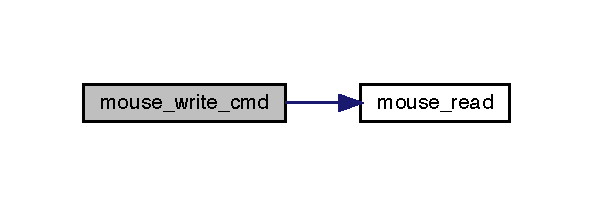
\includegraphics[width=285pt]{group__mouse_gad26aa3828c4a6d900e654de8e4e68e83_cgraph}
\end{center}
\end{figure}

\hypertarget{group___serial}{}\section{Port}
\label{group___serial}\index{Port@{Port}}
\subsection*{Classes}
\begin{DoxyCompactItemize}
\item 
struct \hyperlink{struct_date__t}{Date\+\_\+t}
\begin{DoxyCompactList}\small\item\em Structure used to save a date. \end{DoxyCompactList}\end{DoxyCompactItemize}
\subsection*{Macros}
\begin{DoxyCompactItemize}
\item 
\#define \hyperlink{group___serial_ga3a8ea58898cb58fc96013383d39f482c}{B\+IT}(n)~(0x01$<$$<$(n))
\item 
\#define \hyperlink{group___serial_gaba51915c87d64af47fb1cc59348961c9}{OK}~0
\item 
\#define \hyperlink{group___serial_ga4e22feb6ffbc1cda32fadff5c740dc51}{R\+T\+C\+\_\+\+I\+RQ}~8
\begin{DoxyCompactList}\small\item\em R\+TC I\+RQ line. \end{DoxyCompactList}\item 
\#define \hyperlink{group___serial_gaa03bb5fe5bddcdd5bf15801d73f2c9c2}{R\+T\+C\+\_\+\+I\+N\+I\+T\+I\+A\+L\+\_\+\+H\+O\+O\+K\+\_\+\+ID}~8
\begin{DoxyCompactList}\small\item\em R\+TC Initial hook\+\_\+id. \end{DoxyCompactList}\item 
\#define \hyperlink{group___serial_ga710b98232df2c563009e6f8a6cd18220}{R\+T\+C\+\_\+\+A\+D\+D\+R\+\_\+\+R\+EG}~0x70
\item 
\#define \hyperlink{group___serial_ga2f258a00c59c3f347c8d2d4a75471ce0}{R\+T\+C\+\_\+\+D\+A\+T\+A\+\_\+\+R\+EG}~0x71
\item 
\#define \hyperlink{group___serial_ga98e892db8d518077980341c657099508}{A\+\_\+\+U\+IP}~\hyperlink{group___serial_ga3a8ea58898cb58fc96013383d39f482c}{B\+IT}(7)
\begin{DoxyCompactList}\small\item\em Update in Progress Register. \end{DoxyCompactList}\item 
\#define \hyperlink{group___serial_gaad3e83198dca553658658437932f878e}{A\+\_\+\+D\+V2}~\hyperlink{group___serial_ga3a8ea58898cb58fc96013383d39f482c}{B\+IT}(6)
\begin{DoxyCompactList}\small\item\em D\+V2-\/\+D\+V0 \+: Control the counting chain. \end{DoxyCompactList}\item 
\#define \hyperlink{group___serial_ga4fc9b54f4673ed178656194a52c263c5}{A\+\_\+\+D\+V1}~\hyperlink{group___serial_ga3a8ea58898cb58fc96013383d39f482c}{B\+IT}(5)
\item 
\#define \hyperlink{group___serial_ga571fc22bdbbdc9a64d1592e217b11fcb}{A\+\_\+\+D\+V0}~\hyperlink{group___serial_ga3a8ea58898cb58fc96013383d39f482c}{B\+IT}(4)
\item 
\#define \hyperlink{group___serial_ga89c395dabf3fb44b1bd163e65e0e113a}{A\+\_\+\+R\+S3}~\hyperlink{group___serial_ga3a8ea58898cb58fc96013383d39f482c}{B\+IT}(3)
\begin{DoxyCompactList}\small\item\em R\+S3-\/\+R\+S0 \+: Rate selector. \end{DoxyCompactList}\item 
\#define \hyperlink{group___serial_ga864ddcec6d5b6652d4157f5519c98b32}{A\+\_\+\+R\+S2}~\hyperlink{group___serial_ga3a8ea58898cb58fc96013383d39f482c}{B\+IT}(2)
\item 
\#define \hyperlink{group___serial_ga440f99ae843dfc2cab5148ec88d2a80f}{A\+\_\+\+R\+S1}~\hyperlink{group___serial_ga3a8ea58898cb58fc96013383d39f482c}{B\+IT}(1)
\item 
\#define \hyperlink{group___serial_ga404efd521ab5b53976d3f8cae85db0de}{A\+\_\+\+R\+S0}~\hyperlink{group___serial_ga3a8ea58898cb58fc96013383d39f482c}{B\+IT}(O)
\item 
\#define \hyperlink{group___serial_gab89ee9b74d48a06f138aa6b593a6a7f6}{B\+\_\+\+S\+ET}~\hyperlink{group___serial_ga3a8ea58898cb58fc96013383d39f482c}{B\+IT}(7)
\begin{DoxyCompactList}\small\item\em Inhibit updates of time/date registers. \end{DoxyCompactList}\item 
\#define \hyperlink{group___serial_gac7311a388e3219a525b432d63688f4e4}{B\+\_\+\+P\+IE}~\hyperlink{group___serial_ga3a8ea58898cb58fc96013383d39f482c}{B\+IT}(6)
\begin{DoxyCompactList}\small\item\em Enable Periodic Interrupts. \end{DoxyCompactList}\item 
\#define \hyperlink{group___serial_gaa142656507b3d006de794d8014fe4a58}{B\+\_\+\+A\+EI}~\hyperlink{group___serial_ga3a8ea58898cb58fc96013383d39f482c}{B\+IT}(5)
\begin{DoxyCompactList}\small\item\em Enable Alarm Interrupts. \end{DoxyCompactList}\item 
\#define \hyperlink{group___serial_gad259c663b5ae87d1284556304a6b5961}{B\+\_\+\+U\+EI}~\hyperlink{group___serial_ga3a8ea58898cb58fc96013383d39f482c}{B\+IT}(4)
\begin{DoxyCompactList}\small\item\em Enable Update Interrupts. \end{DoxyCompactList}\item 
\#define \hyperlink{group___serial_ga3e20a5ecd41621ef238af20c871fb8a2}{B\+\_\+\+S\+Q\+WE}~\hyperlink{group___serial_ga3a8ea58898cb58fc96013383d39f482c}{B\+IT}(3)
\begin{DoxyCompactList}\small\item\em Enable square-\/wave generation. \end{DoxyCompactList}\item 
\#define \hyperlink{group___serial_gaf35235826316c655d2ef79122d85ee89}{B\+\_\+\+DM}~\hyperlink{group___serial_ga3a8ea58898cb58fc96013383d39f482c}{B\+IT}(2)
\begin{DoxyCompactList}\small\item\em Set registers in Binary or B\+CD. \end{DoxyCompactList}\item 
\#define \hyperlink{group___serial_ga36493e94586e07546a955df01037e645}{B\+\_\+24\+\_\+12}~\hyperlink{group___serial_ga3a8ea58898cb58fc96013383d39f482c}{B\+IT}(1)
\begin{DoxyCompactList}\small\item\em Set hours range from \mbox{[}0,23\mbox{]} or \mbox{[}0,12\mbox{]}. \end{DoxyCompactList}\item 
\#define \hyperlink{group___serial_ga68191f0d4776566585fbb339c785f8d5}{B\+\_\+\+D\+SE}~\hyperlink{group___serial_ga3a8ea58898cb58fc96013383d39f482c}{B\+IT}(O)
\begin{DoxyCompactList}\small\item\em Enable Daylight Savings Time. \end{DoxyCompactList}\item 
\#define \hyperlink{group___serial_ga100fdbb4db6d90f4b479dc9a2228d90d}{C\+\_\+\+I\+R\+QF}~\hyperlink{group___serial_ga3a8ea58898cb58fc96013383d39f482c}{B\+IT}(7)
\begin{DoxyCompactList}\small\item\em I\+RQ Line Active. \end{DoxyCompactList}\item 
\#define \hyperlink{group___serial_ga05e94124733b6b9a37d3c709e9a99876}{C\+\_\+\+PF}~\hyperlink{group___serial_ga3a8ea58898cb58fc96013383d39f482c}{B\+IT}(6)
\begin{DoxyCompactList}\small\item\em Periodic Interrupt Pending. \end{DoxyCompactList}\item 
\#define \hyperlink{group___serial_gada554ae87b096739211adfc2f59d44f9}{C\+\_\+\+AF}~\hyperlink{group___serial_ga3a8ea58898cb58fc96013383d39f482c}{B\+IT}(5)
\begin{DoxyCompactList}\small\item\em Alarm Interrupt Pending. \end{DoxyCompactList}\item 
\#define \hyperlink{group___serial_gace5b43f703177f892af015bb446486c6}{C\+\_\+\+UE}~\hyperlink{group___serial_ga3a8ea58898cb58fc96013383d39f482c}{B\+IT}(4)
\begin{DoxyCompactList}\small\item\em Update Interrupt Pending. \end{DoxyCompactList}\item 
\#define \hyperlink{group___serial_gad37cf3225412330f91c3fb21b2611109}{D\+\_\+\+V\+RT}~\hyperlink{group___serial_ga3a8ea58898cb58fc96013383d39f482c}{B\+IT}(7)
\begin{DoxyCompactList}\small\item\em Valid Time. \end{DoxyCompactList}\item 
\#define \hyperlink{group___serial_gaff232d9a767044ad7e38751aa010880c}{A\+L\+\_\+\+S\+E\+C\+O\+N\+DS}~0\+X00
\begin{DoxyCompactList}\small\item\em Seconds. \end{DoxyCompactList}\item 
\#define \hyperlink{group___serial_ga9199a39ddfac98d39cf38c11dce52b67}{A\+L\+\_\+\+S\+E\+C\+\_\+\+A\+L\+A\+RM}~0\+X01
\begin{DoxyCompactList}\small\item\em Seconds Alarm. \end{DoxyCompactList}\item 
\#define \hyperlink{group___serial_ga71c9c535bfcb21a9523f93f849253e57}{A\+L\+\_\+\+M\+I\+N\+U\+T\+ES}~0\+X02
\begin{DoxyCompactList}\small\item\em Minutes. \end{DoxyCompactList}\item 
\#define \hyperlink{group___serial_ga9b3e0bfebdc40a726066400d65dce101}{A\+L\+\_\+\+M\+I\+N\+\_\+\+A\+L\+A\+RM}~0\+X03
\begin{DoxyCompactList}\small\item\em Minutes Alarm. \end{DoxyCompactList}\item 
\#define \hyperlink{group___serial_ga3c46c3b006367d25664bae636198069c}{A\+L\+\_\+\+H\+O\+U\+RS}~0\+X04
\begin{DoxyCompactList}\small\item\em Hours (12-\/hour or 24-\/hour mode) \end{DoxyCompactList}\item 
\#define \hyperlink{group___serial_gab46bf2cfed82e0746ac9a234744fbb10}{A\+L\+\_\+\+H\+O\+U\+R\+S\+\_\+\+A\+L\+A\+R\+AM}~0\+X05
\begin{DoxyCompactList}\small\item\em Hours Alarm. \end{DoxyCompactList}\item 
\#define \hyperlink{group___serial_gaacd25fdddd522fbf292e61e26c3c442f}{A\+L\+\_\+\+D\+A\+Y\+\_\+\+O\+F\+\_\+\+W\+E\+EK}~0x06
\begin{DoxyCompactList}\small\item\em Day of the Week (Sunday = 1) \end{DoxyCompactList}\item 
\#define \hyperlink{group___serial_gaa60f550f2d0cc5a3fe5177039150bc60}{A\+L\+\_\+\+D\+AY}~0x07
\begin{DoxyCompactList}\small\item\em Day of the Month. \end{DoxyCompactList}\item 
\#define \hyperlink{group___serial_gaf660f603c1c09d1bf76a4367ddba440b}{A\+L\+\_\+\+M\+O\+N\+TH}~0x08
\begin{DoxyCompactList}\small\item\em Month. \end{DoxyCompactList}\item 
\#define \hyperlink{group___serial_ga05557977458cf6879226d194bb46538f}{A\+L\+\_\+\+Y\+E\+AR}~0x09
\begin{DoxyCompactList}\small\item\em Year. \end{DoxyCompactList}\item 
\#define \hyperlink{group___serial_ga8c4718b100d35ffbc2b5a753e4a700ab}{A\+L\+\_\+\+R\+E\+GA}~0x0A
\begin{DoxyCompactList}\small\item\em Control Register A. \end{DoxyCompactList}\item 
\#define \hyperlink{group___serial_ga404629cba65787d7e69df3b23d84aa2a}{A\+L\+\_\+\+R\+E\+GB}~0x0B
\begin{DoxyCompactList}\small\item\em Control Register B. \end{DoxyCompactList}\item 
\#define \hyperlink{group___serial_ga208d2a2e644c42d00b0a348b6635c4c5}{A\+L\+\_\+\+R\+E\+GC}~0x0C
\begin{DoxyCompactList}\small\item\em Control Register C. \end{DoxyCompactList}\item 
\#define \hyperlink{group___serial_gaa15a8cf99dbd75d8127ff660c71460f2}{A\+L\+\_\+\+R\+E\+GD}~0x0D
\begin{DoxyCompactList}\small\item\em Control Register. \end{DoxyCompactList}\item 
\#define \hyperlink{group___serial_ga3a8ea58898cb58fc96013383d39f482c}{B\+IT}(n)~(0x01$<$$<$(n))
\item 
\#define \hyperlink{group___serial_gaba51915c87d64af47fb1cc59348961c9}{OK}~0
\item 
\#define \hyperlink{group___serial_ga3685c78b9bd6dd0fa3861807e24a4e1b}{C\+O\+M1\+\_\+\+I\+RQ}~4
\item 
\#define \hyperlink{group___serial_gab02d84052a299a0c207a8ea4c1a5636d}{C\+O\+M2\+\_\+\+I\+RQ}~3
\item 
\#define \hyperlink{group___serial_ga8982f081d8608e775b0739cde65373d5}{C\+O\+M1\+\_\+\+P\+O\+RT}~0x3\+F8
\item 
\#define \hyperlink{group___serial_ga88373c3e34a242356333ec08389eae54}{C\+O\+M2\+\_\+\+P\+O\+RT}~0x2\+F8
\item 
\#define \hyperlink{group___serial_ga562471a291b13121258a12d45f1679ce}{S\+E\+R\+I\+A\+L\+\_\+\+I\+N\+I\+T\+I\+A\+L\+\_\+\+H\+O\+O\+K\+\_\+\+ID}~4
\item 
\#define \hyperlink{group___serial_gaa6f7e7a9f4551d6151f9d45362118a50}{R\+BR}~0x00
\begin{DoxyCompactList}\small\item\em Receiver Buffer Register -\/ Read. \end{DoxyCompactList}\item 
\#define \hyperlink{group___serial_ga5e9787adf3c9afcc4b781e85bb545b35}{T\+HR}~0x00
\begin{DoxyCompactList}\small\item\em Transmitter Holding Register -\/ Write. \end{DoxyCompactList}\item 
\#define \hyperlink{group___serial_ga3e27fa35f9febccdc4a0c28a5c8cffbb}{I\+ER}~0x01
\begin{DoxyCompactList}\small\item\em Interrupt Enable Register -\/ Read/ Write. \end{DoxyCompactList}\item 
\#define \hyperlink{group___serial_ga67004975983f9c99226d63db17ba74c4}{I\+IR}~0x02
\begin{DoxyCompactList}\small\item\em Interrupt Indentification Reg. -\/ Read. \end{DoxyCompactList}\item 
\#define \hyperlink{group___serial_ga264b36b13386e3f62fe69e04711bc006}{F\+CR}~0x02
\begin{DoxyCompactList}\small\item\em F\+I\+FO Control Register -\/ Write. \end{DoxyCompactList}\item 
\#define \hyperlink{group___serial_ga851cb396b6eaa97346364a772b439f37}{L\+CR}~0x03
\begin{DoxyCompactList}\small\item\em Line Control Register -\/ Read/ Write. \end{DoxyCompactList}\item 
\#define \hyperlink{group___serial_ga65364db1603cde6f6533cb61bcfcf553}{M\+CR}~0x04
\begin{DoxyCompactList}\small\item\em Modem Control Register -\/ Read/ Write. \end{DoxyCompactList}\item 
\#define \hyperlink{group___serial_gad51d51aee21f6cc77d4955221aee3dcb}{L\+SR}~0x05
\begin{DoxyCompactList}\small\item\em Line Status Register -\/ Read. \end{DoxyCompactList}\item 
\#define \hyperlink{group___serial_gad4806a0bfd996121bc27d2466393207e}{M\+SR}~0x06
\begin{DoxyCompactList}\small\item\em Modem Status Register -\/ Read. \end{DoxyCompactList}\item 
\#define \hyperlink{group___serial_gabaed93a16a0cde13f32bc4dc48b96804}{SR}~0x07
\begin{DoxyCompactList}\small\item\em Scratchpad Register -\/ Read/ Write. \end{DoxyCompactList}\item 
\#define \hyperlink{group___serial_ga4466639cd64ebf372a621168c5e25964}{D\+LL}~0x00
\begin{DoxyCompactList}\small\item\em Divisor Latch L\+SB. \end{DoxyCompactList}\item 
\#define \hyperlink{group___serial_ga3b48b12dc65f62dd40ab1163fe7997fb}{D\+LM}~0x01
\begin{DoxyCompactList}\small\item\em Divisor Latch M\+SB. \end{DoxyCompactList}\item 
\#define \hyperlink{group___serial_ga16e7001a19bba69533659ff82cbead08}{S\+E\+R\+I\+A\+L\+\_\+\+B\+I\+T\+\_\+\+R\+A\+TE}~19200
\item 
\#define \hyperlink{group___serial_ga5a02cec014399767cbb673100ccfa3f8}{S\+E\+R\+I\+A\+L\+\_\+\+B\+A\+S\+E\+\_\+\+BR}~115200
\item 
\#define \hyperlink{group___serial_ga1cf80a668c79b3081803063178f40920}{L\+C\+R\+\_\+\+D\+L\+AB}~\hyperlink{group___serial_ga3a8ea58898cb58fc96013383d39f482c}{B\+IT}(7)
\begin{DoxyCompactList}\small\item\em Divisor Latch Access. \end{DoxyCompactList}\item 
\#define \hyperlink{group___serial_ga896faa6ed28b750f3a5b9927ea12aedb}{L\+C\+R\+\_\+\+BC}~\hyperlink{group___serial_ga3a8ea58898cb58fc96013383d39f482c}{B\+IT}(6)
\begin{DoxyCompactList}\small\item\em Break Control. \end{DoxyCompactList}\item 
\#define \hyperlink{group___serial_ga5e6060e38b2ad74954b34f6ac82b8a5b}{L\+C\+R\+\_\+\+P\+C2}~\hyperlink{group___serial_ga3a8ea58898cb58fc96013383d39f482c}{B\+IT}(5)
\begin{DoxyCompactList}\small\item\em Parity Control. \end{DoxyCompactList}\item 
\#define \hyperlink{group___serial_ga6ab1327cf213d22d2acc07b397c85f0f}{L\+C\+R\+\_\+\+P\+C1}~\hyperlink{group___serial_ga3a8ea58898cb58fc96013383d39f482c}{B\+IT}(4)
\begin{DoxyCompactList}\small\item\em Parity Control. \end{DoxyCompactList}\item 
\#define \hyperlink{group___serial_ga5b25ad27007f83425b63a30298743f01}{L\+C\+R\+\_\+\+P\+C0}~\hyperlink{group___serial_ga3a8ea58898cb58fc96013383d39f482c}{B\+IT}(3)
\begin{DoxyCompactList}\small\item\em Parity Control. \end{DoxyCompactList}\item 
\#define \hyperlink{group___serial_ga9d59a56595a0f0c5af42cab8a9d3a656}{L\+C\+R\+\_\+\+SB}~\hyperlink{group___serial_ga3a8ea58898cb58fc96013383d39f482c}{B\+IT}(2)
\begin{DoxyCompactList}\small\item\em Stop Bit. \end{DoxyCompactList}\item 
\#define \hyperlink{group___serial_ga4271f672ad1c921995a3868074747d19}{L\+C\+R\+\_\+\+B\+P\+C1}~\hyperlink{group___serial_ga3a8ea58898cb58fc96013383d39f482c}{B\+IT}(1)
\begin{DoxyCompactList}\small\item\em Number of bits per char. \end{DoxyCompactList}\item 
\#define \hyperlink{group___serial_gae82a6d40fb6637ebdea0cf527594c3fc}{L\+C\+R\+\_\+\+B\+P\+C0}~\hyperlink{group___serial_ga3a8ea58898cb58fc96013383d39f482c}{B\+IT}(0)
\begin{DoxyCompactList}\small\item\em Number of bits per char. \end{DoxyCompactList}\item 
\#define \hyperlink{group___serial_ga17abffa14207797fba6c62875367d085}{L\+S\+R\+\_\+\+F\+I\+F\+O\+\_\+E}~\hyperlink{group___serial_ga3a8ea58898cb58fc96013383d39f482c}{B\+IT}(7)
\begin{DoxyCompactList}\small\item\em F\+I\+FO with Errors. \end{DoxyCompactList}\item 
\#define \hyperlink{group___serial_ga6b9fdb38c6b844ba25a7dba0f024e20c}{L\+S\+R\+\_\+\+T\+ER}~\hyperlink{group___serial_ga3a8ea58898cb58fc96013383d39f482c}{B\+IT}(6)
\begin{DoxyCompactList}\small\item\em Transmitter Empty Register. \end{DoxyCompactList}\item 
\#define \hyperlink{group___serial_ga8c1a828f5fe296a9c1668cf3e72c00c1}{L\+S\+R\+\_\+\+T\+H\+RE}~\hyperlink{group___serial_ga3a8ea58898cb58fc96013383d39f482c}{B\+IT}(5)
\begin{DoxyCompactList}\small\item\em Transmitter Holding Register Empty. \end{DoxyCompactList}\item 
\#define \hyperlink{group___serial_ga0fa2f414cac085b768774f2881321b60}{L\+S\+R\+\_\+\+BI}~\hyperlink{group___serial_ga3a8ea58898cb58fc96013383d39f482c}{B\+IT}(4)
\begin{DoxyCompactList}\small\item\em Break Interrupt. \end{DoxyCompactList}\item 
\#define \hyperlink{group___serial_gae3f9ccc88c615d1257ad400cf27af7eb}{L\+S\+R\+\_\+\+FE}~\hyperlink{group___serial_ga3a8ea58898cb58fc96013383d39f482c}{B\+IT}(3)
\begin{DoxyCompactList}\small\item\em Framing Error. \end{DoxyCompactList}\item 
\#define \hyperlink{group___serial_ga0ee28cdbc0917173f06cc39527452a8f}{L\+S\+R\+\_\+\+PE}~\hyperlink{group___serial_ga3a8ea58898cb58fc96013383d39f482c}{B\+IT}(2)
\begin{DoxyCompactList}\small\item\em Parity Error. \end{DoxyCompactList}\item 
\#define \hyperlink{group___serial_gae844dd49bb0e0770bcf46ad5bfe20973}{L\+S\+R\+\_\+\+OE}~\hyperlink{group___serial_ga3a8ea58898cb58fc96013383d39f482c}{B\+IT}(1)
\begin{DoxyCompactList}\small\item\em Overrun Error. \end{DoxyCompactList}\item 
\#define \hyperlink{group___serial_gaef6b74ebb13843a65360fd9150bfe60f}{L\+S\+R\+\_\+\+RD}~\hyperlink{group___serial_ga3a8ea58898cb58fc96013383d39f482c}{B\+IT}(0)
\begin{DoxyCompactList}\small\item\em Receiver is Ready. \end{DoxyCompactList}\item 
\#define \hyperlink{group___serial_gae06fe45719e515d431ec3b0e9356516d}{I\+E\+R\+\_\+\+M\+O\+D\+EM}~\hyperlink{group___serial_ga3a8ea58898cb58fc96013383d39f482c}{B\+IT}(3)
\begin{DoxyCompactList}\small\item\em Enables the M\+O\+D\+EM Status Interrupt. \end{DoxyCompactList}\item 
\#define \hyperlink{group___serial_gaec947c63128590c8f615862ee9c2c953}{I\+E\+R\+\_\+\+R\+LS}~\hyperlink{group___serial_ga3a8ea58898cb58fc96013383d39f482c}{B\+IT}(2)
\begin{DoxyCompactList}\small\item\em Enables the Receiver Line Status Interrupt. \end{DoxyCompactList}\item 
\#define \hyperlink{group___serial_ga22682c3d4571d7a79ed0ca2bc88a15a6}{I\+E\+R\+\_\+\+T\+H\+RE}~\hyperlink{group___serial_ga3a8ea58898cb58fc96013383d39f482c}{B\+IT}(1)
\begin{DoxyCompactList}\small\item\em Enables the Transmitter Holding Register Empty Interrupt. \end{DoxyCompactList}\item 
\#define \hyperlink{group___serial_gacc2bd3737c0687e576384afc1a37a0cc}{I\+E\+R\+\_\+\+R\+DA}~\hyperlink{group___serial_ga3a8ea58898cb58fc96013383d39f482c}{B\+IT}(0)
\begin{DoxyCompactList}\small\item\em Enables the R\+Eceived Data Available Interrupt. \end{DoxyCompactList}\item 
\#define \hyperlink{group___serial_ga62a27224c8cece6052419d605737fd1e}{I\+I\+R\+\_\+\+I\+P2}~\hyperlink{group___serial_ga3a8ea58898cb58fc96013383d39f482c}{B\+IT}(3)
\begin{DoxyCompactList}\small\item\em Pending Interrupts Information. \end{DoxyCompactList}\item 
\#define \hyperlink{group___serial_ga25fc1de85f4df9dc8249e52bdc25f73d}{I\+I\+R\+\_\+\+I\+P1}~\hyperlink{group___serial_ga3a8ea58898cb58fc96013383d39f482c}{B\+IT}(2)
\begin{DoxyCompactList}\small\item\em Pending Interrupts Information. \end{DoxyCompactList}\item 
\#define \hyperlink{group___serial_ga404030d0e2acaec8bd39b8a9b01daf83}{I\+I\+R\+\_\+\+I\+P0}~\hyperlink{group___serial_ga3a8ea58898cb58fc96013383d39f482c}{B\+IT}(1)
\begin{DoxyCompactList}\small\item\em Pending Interrupts Information. \end{DoxyCompactList}\item 
\#define \hyperlink{group___serial_ga801f50fdaed5e1d41cc8606b06a4f993}{I\+I\+R\+\_\+\+N\+PI}~\hyperlink{group___serial_ga3a8ea58898cb58fc96013383d39f482c}{B\+IT}(0)
\begin{DoxyCompactList}\small\item\em Non Pending Interrupts. \end{DoxyCompactList}\item 
\#define \hyperlink{group___serial_gadd8802975b6d7cbf87ae7fcf8256baa2}{F\+I\+F\+O\+\_\+\+R\+C\+V\+R1}~\hyperlink{group___serial_ga3a8ea58898cb58fc96013383d39f482c}{B\+IT}(7)
\begin{DoxyCompactList}\small\item\em R\+C\+VR F\+I\+FO Trigger Level (Bytes) (for 16 byte F\+I\+F\+Os) \end{DoxyCompactList}\item 
\#define \hyperlink{group___serial_ga10947413fec5094d1e649a4764ce752a}{F\+I\+F\+O\+\_\+\+R\+C\+V\+R2}~\hyperlink{group___serial_ga3a8ea58898cb58fc96013383d39f482c}{B\+IT}(6)
\begin{DoxyCompactList}\small\item\em R\+C\+VR F\+I\+FO Trigger Level (Bytes) (for 16 byte F\+I\+F\+Os) \end{DoxyCompactList}\item 
\#define \hyperlink{group___serial_ga870d1e13c64ab331ab0ddabd53f8f6dc}{F\+I\+F\+O\+\_\+\+E\+N64}~\hyperlink{group___serial_ga3a8ea58898cb58fc96013383d39f482c}{B\+IT}(5)
\begin{DoxyCompactList}\small\item\em Enable 64 byte F\+I\+FO. \end{DoxyCompactList}\item 
\#define \hyperlink{group___serial_ga04cb242ce6c87c7e317544b69e213eeb}{F\+I\+F\+O\+\_\+\+CX}~\hyperlink{group___serial_ga3a8ea58898cb58fc96013383d39f482c}{B\+IT}(2)
\begin{DoxyCompactList}\small\item\em Clear bytes in X\+M\+IT F\+I\+FO. \end{DoxyCompactList}\item 
\#define \hyperlink{group___serial_gaf6a8e6e80294a60dfd5f39cf965c4a13}{F\+I\+F\+O\+\_\+\+CR}~\hyperlink{group___serial_ga3a8ea58898cb58fc96013383d39f482c}{B\+IT}(1)
\begin{DoxyCompactList}\small\item\em Clear bytes in R\+C\+VR F\+I\+FO. \end{DoxyCompactList}\item 
\#define \hyperlink{group___serial_ga53954ec7f9dc790f00548da08ccd5ed6}{F\+I\+F\+O\+\_\+\+EN}~\hyperlink{group___serial_ga3a8ea58898cb58fc96013383d39f482c}{B\+IT}(0)
\begin{DoxyCompactList}\small\item\em Enable both F\+I\+FO\textquotesingle{}s. \end{DoxyCompactList}\end{DoxyCompactItemize}
\subsection*{Functions}
\begin{DoxyCompactItemize}
\item 
int \hyperlink{group___serial_gab77fc689b79cf1fa098f71a4ff5abdeb}{parser\+B\+CD} (int value)
\item 
int \hyperlink{group___serial_ga50431f28993883d49a09ce054bd5c0ec}{rtc\+\_\+read\+\_\+register} (int reg)
\begin{DoxyCompactList}\small\item\em (From Assembly) Reads Value from register reg \end{DoxyCompactList}\item 
int \hyperlink{group___serial_ga6bd13bd1e0cd043f50abb97bcc138bfa}{rtc\+\_\+subscribe\+\_\+int} (void)
\begin{DoxyCompactList}\small\item\em Subscribes and enables R\+TC interrupts. \end{DoxyCompactList}\item 
int \hyperlink{group___serial_ga5b1cba4be2c15183b9f2c089fe6e946a}{rtc\+\_\+unsubscribe\+\_\+int} (void)
\begin{DoxyCompactList}\small\item\em Unsubscribes R\+TC interrupts. \end{DoxyCompactList}\item 
int \hyperlink{group___serial_gab88c07eaefdae0ccbae9e7c2a1e04f71}{rtc\+\_\+write\+\_\+register} (unsigned long reg, unsigned long value)
\begin{DoxyCompactList}\small\item\em Writes value to register reg. \end{DoxyCompactList}\item 
int \hyperlink{group___serial_gacaae78073772a1f95560e42cef087a93}{rtc\+\_\+updating} (void)
\item 
\hyperlink{struct_date__t}{Date\+\_\+t} $\ast$ \hyperlink{group___serial_ga08a02c163edf9dc74b2d15dfb23a2624}{rtc\+\_\+read\+\_\+date} (void)
\item 
int \hyperlink{group___serial_ga31328528e82730ef05d9e6121447dd42}{serial\+\_\+subscribe\+\_\+int} (void)
\begin{DoxyCompactList}\small\item\em Subscribes and enables Serial Port interrupts. \end{DoxyCompactList}\item 
int \hyperlink{group___serial_ga56e227db9f0a79bfb5fd8a753d1be67a}{serial\+\_\+unsubscribe\+\_\+int} (void)
\begin{DoxyCompactList}\small\item\em Unsubscribes Serial Port interrupts. \end{DoxyCompactList}\item 
int \hyperlink{group___serial_ga06724a3064e96e445257aba1e4f3de46}{serial\+\_\+enable\+\_\+interrupts} ()
\begin{DoxyCompactList}\small\item\em Enables Interrupt Mode for the Serial Port. \end{DoxyCompactList}\item 
int \hyperlink{group___serial_gab84b5f47451f228a5c574b77e5c7e9eb}{serial\+\_\+disable\+\_\+interrupts} ()
\begin{DoxyCompactList}\small\item\em Disables Interruptions in the Serial Port. \end{DoxyCompactList}\item 
int \hyperlink{group___serial_ga78786e639e5d536f1c65170e7396fde6}{serial\+\_\+set\+\_\+conf} ()
\begin{DoxyCompactList}\small\item\em Sets the desired configuration of the U\+A\+RT registers. \end{DoxyCompactList}\item 
unsigned char \hyperlink{group___serial_ga733df3cf88f5c81a1c4ae2822342dd2d}{serial\+\_\+read} ()
\begin{DoxyCompactList}\small\item\em Reads information received using the serial port. \end{DoxyCompactList}\item 
int \hyperlink{group___serial_ga62f6ef11a701d503d1ed5f4a873a1d2b}{serial\+\_\+write} (unsigned char info)
\begin{DoxyCompactList}\small\item\em Sends information using the serial port. \end{DoxyCompactList}\end{DoxyCompactItemize}


\subsection{Detailed Description}
Functions for using the R\+TC -\/ Real Time Clock

Functions for using the Serial Port 

\subsection{Macro Definition Documentation}
\hypertarget{group___serial_ga571fc22bdbbdc9a64d1592e217b11fcb}{}\label{group___serial_ga571fc22bdbbdc9a64d1592e217b11fcb} 
\index{Port@{Port}!A\+\_\+\+D\+V0@{A\+\_\+\+D\+V0}}
\index{A\+\_\+\+D\+V0@{A\+\_\+\+D\+V0}!Port@{Port}}
\subsubsection{\texorpdfstring{A\+\_\+\+D\+V0}{A\_DV0}}
{\footnotesize\ttfamily \#define A\+\_\+\+D\+V0~\hyperlink{group___serial_ga3a8ea58898cb58fc96013383d39f482c}{B\+IT}(4)}

\hypertarget{group___serial_ga4fc9b54f4673ed178656194a52c263c5}{}\label{group___serial_ga4fc9b54f4673ed178656194a52c263c5} 
\index{Port@{Port}!A\+\_\+\+D\+V1@{A\+\_\+\+D\+V1}}
\index{A\+\_\+\+D\+V1@{A\+\_\+\+D\+V1}!Port@{Port}}
\subsubsection{\texorpdfstring{A\+\_\+\+D\+V1}{A\_DV1}}
{\footnotesize\ttfamily \#define A\+\_\+\+D\+V1~\hyperlink{group___serial_ga3a8ea58898cb58fc96013383d39f482c}{B\+IT}(5)}

\hypertarget{group___serial_gaad3e83198dca553658658437932f878e}{}\label{group___serial_gaad3e83198dca553658658437932f878e} 
\index{Port@{Port}!A\+\_\+\+D\+V2@{A\+\_\+\+D\+V2}}
\index{A\+\_\+\+D\+V2@{A\+\_\+\+D\+V2}!Port@{Port}}
\subsubsection{\texorpdfstring{A\+\_\+\+D\+V2}{A\_DV2}}
{\footnotesize\ttfamily \#define A\+\_\+\+D\+V2~\hyperlink{group___serial_ga3a8ea58898cb58fc96013383d39f482c}{B\+IT}(6)}



D\+V2-\/\+D\+V0 \+: Control the counting chain. 

\hypertarget{group___serial_ga404efd521ab5b53976d3f8cae85db0de}{}\label{group___serial_ga404efd521ab5b53976d3f8cae85db0de} 
\index{Port@{Port}!A\+\_\+\+R\+S0@{A\+\_\+\+R\+S0}}
\index{A\+\_\+\+R\+S0@{A\+\_\+\+R\+S0}!Port@{Port}}
\subsubsection{\texorpdfstring{A\+\_\+\+R\+S0}{A\_RS0}}
{\footnotesize\ttfamily \#define A\+\_\+\+R\+S0~\hyperlink{group___serial_ga3a8ea58898cb58fc96013383d39f482c}{B\+IT}(O)}

\hypertarget{group___serial_ga440f99ae843dfc2cab5148ec88d2a80f}{}\label{group___serial_ga440f99ae843dfc2cab5148ec88d2a80f} 
\index{Port@{Port}!A\+\_\+\+R\+S1@{A\+\_\+\+R\+S1}}
\index{A\+\_\+\+R\+S1@{A\+\_\+\+R\+S1}!Port@{Port}}
\subsubsection{\texorpdfstring{A\+\_\+\+R\+S1}{A\_RS1}}
{\footnotesize\ttfamily \#define A\+\_\+\+R\+S1~\hyperlink{group___serial_ga3a8ea58898cb58fc96013383d39f482c}{B\+IT}(1)}

\hypertarget{group___serial_ga864ddcec6d5b6652d4157f5519c98b32}{}\label{group___serial_ga864ddcec6d5b6652d4157f5519c98b32} 
\index{Port@{Port}!A\+\_\+\+R\+S2@{A\+\_\+\+R\+S2}}
\index{A\+\_\+\+R\+S2@{A\+\_\+\+R\+S2}!Port@{Port}}
\subsubsection{\texorpdfstring{A\+\_\+\+R\+S2}{A\_RS2}}
{\footnotesize\ttfamily \#define A\+\_\+\+R\+S2~\hyperlink{group___serial_ga3a8ea58898cb58fc96013383d39f482c}{B\+IT}(2)}

\hypertarget{group___serial_ga89c395dabf3fb44b1bd163e65e0e113a}{}\label{group___serial_ga89c395dabf3fb44b1bd163e65e0e113a} 
\index{Port@{Port}!A\+\_\+\+R\+S3@{A\+\_\+\+R\+S3}}
\index{A\+\_\+\+R\+S3@{A\+\_\+\+R\+S3}!Port@{Port}}
\subsubsection{\texorpdfstring{A\+\_\+\+R\+S3}{A\_RS3}}
{\footnotesize\ttfamily \#define A\+\_\+\+R\+S3~\hyperlink{group___serial_ga3a8ea58898cb58fc96013383d39f482c}{B\+IT}(3)}



R\+S3-\/\+R\+S0 \+: Rate selector. 

\hypertarget{group___serial_ga98e892db8d518077980341c657099508}{}\label{group___serial_ga98e892db8d518077980341c657099508} 
\index{Port@{Port}!A\+\_\+\+U\+IP@{A\+\_\+\+U\+IP}}
\index{A\+\_\+\+U\+IP@{A\+\_\+\+U\+IP}!Port@{Port}}
\subsubsection{\texorpdfstring{A\+\_\+\+U\+IP}{A\_UIP}}
{\footnotesize\ttfamily \#define A\+\_\+\+U\+IP~\hyperlink{group___serial_ga3a8ea58898cb58fc96013383d39f482c}{B\+IT}(7)}



Update in Progress Register. 

\hypertarget{group___serial_gaa60f550f2d0cc5a3fe5177039150bc60}{}\label{group___serial_gaa60f550f2d0cc5a3fe5177039150bc60} 
\index{Port@{Port}!A\+L\+\_\+\+D\+AY@{A\+L\+\_\+\+D\+AY}}
\index{A\+L\+\_\+\+D\+AY@{A\+L\+\_\+\+D\+AY}!Port@{Port}}
\subsubsection{\texorpdfstring{A\+L\+\_\+\+D\+AY}{AL\_DAY}}
{\footnotesize\ttfamily \#define A\+L\+\_\+\+D\+AY~0x07}



Day of the Month. 

\hypertarget{group___serial_gaacd25fdddd522fbf292e61e26c3c442f}{}\label{group___serial_gaacd25fdddd522fbf292e61e26c3c442f} 
\index{Port@{Port}!A\+L\+\_\+\+D\+A\+Y\+\_\+\+O\+F\+\_\+\+W\+E\+EK@{A\+L\+\_\+\+D\+A\+Y\+\_\+\+O\+F\+\_\+\+W\+E\+EK}}
\index{A\+L\+\_\+\+D\+A\+Y\+\_\+\+O\+F\+\_\+\+W\+E\+EK@{A\+L\+\_\+\+D\+A\+Y\+\_\+\+O\+F\+\_\+\+W\+E\+EK}!Port@{Port}}
\subsubsection{\texorpdfstring{A\+L\+\_\+\+D\+A\+Y\+\_\+\+O\+F\+\_\+\+W\+E\+EK}{AL\_DAY\_OF\_WEEK}}
{\footnotesize\ttfamily \#define A\+L\+\_\+\+D\+A\+Y\+\_\+\+O\+F\+\_\+\+W\+E\+EK~0x06}



Day of the Week (Sunday = 1) 

\hypertarget{group___serial_ga3c46c3b006367d25664bae636198069c}{}\label{group___serial_ga3c46c3b006367d25664bae636198069c} 
\index{Port@{Port}!A\+L\+\_\+\+H\+O\+U\+RS@{A\+L\+\_\+\+H\+O\+U\+RS}}
\index{A\+L\+\_\+\+H\+O\+U\+RS@{A\+L\+\_\+\+H\+O\+U\+RS}!Port@{Port}}
\subsubsection{\texorpdfstring{A\+L\+\_\+\+H\+O\+U\+RS}{AL\_HOURS}}
{\footnotesize\ttfamily \#define A\+L\+\_\+\+H\+O\+U\+RS~0\+X04}



Hours (12-\/hour or 24-\/hour mode) 

\hypertarget{group___serial_gab46bf2cfed82e0746ac9a234744fbb10}{}\label{group___serial_gab46bf2cfed82e0746ac9a234744fbb10} 
\index{Port@{Port}!A\+L\+\_\+\+H\+O\+U\+R\+S\+\_\+\+A\+L\+A\+R\+AM@{A\+L\+\_\+\+H\+O\+U\+R\+S\+\_\+\+A\+L\+A\+R\+AM}}
\index{A\+L\+\_\+\+H\+O\+U\+R\+S\+\_\+\+A\+L\+A\+R\+AM@{A\+L\+\_\+\+H\+O\+U\+R\+S\+\_\+\+A\+L\+A\+R\+AM}!Port@{Port}}
\subsubsection{\texorpdfstring{A\+L\+\_\+\+H\+O\+U\+R\+S\+\_\+\+A\+L\+A\+R\+AM}{AL\_HOURS\_ALARAM}}
{\footnotesize\ttfamily \#define A\+L\+\_\+\+H\+O\+U\+R\+S\+\_\+\+A\+L\+A\+R\+AM~0\+X05}



Hours Alarm. 

\hypertarget{group___serial_ga9b3e0bfebdc40a726066400d65dce101}{}\label{group___serial_ga9b3e0bfebdc40a726066400d65dce101} 
\index{Port@{Port}!A\+L\+\_\+\+M\+I\+N\+\_\+\+A\+L\+A\+RM@{A\+L\+\_\+\+M\+I\+N\+\_\+\+A\+L\+A\+RM}}
\index{A\+L\+\_\+\+M\+I\+N\+\_\+\+A\+L\+A\+RM@{A\+L\+\_\+\+M\+I\+N\+\_\+\+A\+L\+A\+RM}!Port@{Port}}
\subsubsection{\texorpdfstring{A\+L\+\_\+\+M\+I\+N\+\_\+\+A\+L\+A\+RM}{AL\_MIN\_ALARM}}
{\footnotesize\ttfamily \#define A\+L\+\_\+\+M\+I\+N\+\_\+\+A\+L\+A\+RM~0\+X03}



Minutes Alarm. 

\hypertarget{group___serial_ga71c9c535bfcb21a9523f93f849253e57}{}\label{group___serial_ga71c9c535bfcb21a9523f93f849253e57} 
\index{Port@{Port}!A\+L\+\_\+\+M\+I\+N\+U\+T\+ES@{A\+L\+\_\+\+M\+I\+N\+U\+T\+ES}}
\index{A\+L\+\_\+\+M\+I\+N\+U\+T\+ES@{A\+L\+\_\+\+M\+I\+N\+U\+T\+ES}!Port@{Port}}
\subsubsection{\texorpdfstring{A\+L\+\_\+\+M\+I\+N\+U\+T\+ES}{AL\_MINUTES}}
{\footnotesize\ttfamily \#define A\+L\+\_\+\+M\+I\+N\+U\+T\+ES~0\+X02}



Minutes. 

\hypertarget{group___serial_gaf660f603c1c09d1bf76a4367ddba440b}{}\label{group___serial_gaf660f603c1c09d1bf76a4367ddba440b} 
\index{Port@{Port}!A\+L\+\_\+\+M\+O\+N\+TH@{A\+L\+\_\+\+M\+O\+N\+TH}}
\index{A\+L\+\_\+\+M\+O\+N\+TH@{A\+L\+\_\+\+M\+O\+N\+TH}!Port@{Port}}
\subsubsection{\texorpdfstring{A\+L\+\_\+\+M\+O\+N\+TH}{AL\_MONTH}}
{\footnotesize\ttfamily \#define A\+L\+\_\+\+M\+O\+N\+TH~0x08}



Month. 

\hypertarget{group___serial_ga8c4718b100d35ffbc2b5a753e4a700ab}{}\label{group___serial_ga8c4718b100d35ffbc2b5a753e4a700ab} 
\index{Port@{Port}!A\+L\+\_\+\+R\+E\+GA@{A\+L\+\_\+\+R\+E\+GA}}
\index{A\+L\+\_\+\+R\+E\+GA@{A\+L\+\_\+\+R\+E\+GA}!Port@{Port}}
\subsubsection{\texorpdfstring{A\+L\+\_\+\+R\+E\+GA}{AL\_REGA}}
{\footnotesize\ttfamily \#define A\+L\+\_\+\+R\+E\+GA~0x0A}



Control Register A. 

\hypertarget{group___serial_ga404629cba65787d7e69df3b23d84aa2a}{}\label{group___serial_ga404629cba65787d7e69df3b23d84aa2a} 
\index{Port@{Port}!A\+L\+\_\+\+R\+E\+GB@{A\+L\+\_\+\+R\+E\+GB}}
\index{A\+L\+\_\+\+R\+E\+GB@{A\+L\+\_\+\+R\+E\+GB}!Port@{Port}}
\subsubsection{\texorpdfstring{A\+L\+\_\+\+R\+E\+GB}{AL\_REGB}}
{\footnotesize\ttfamily \#define A\+L\+\_\+\+R\+E\+GB~0x0B}



Control Register B. 

\hypertarget{group___serial_ga208d2a2e644c42d00b0a348b6635c4c5}{}\label{group___serial_ga208d2a2e644c42d00b0a348b6635c4c5} 
\index{Port@{Port}!A\+L\+\_\+\+R\+E\+GC@{A\+L\+\_\+\+R\+E\+GC}}
\index{A\+L\+\_\+\+R\+E\+GC@{A\+L\+\_\+\+R\+E\+GC}!Port@{Port}}
\subsubsection{\texorpdfstring{A\+L\+\_\+\+R\+E\+GC}{AL\_REGC}}
{\footnotesize\ttfamily \#define A\+L\+\_\+\+R\+E\+GC~0x0C}



Control Register C. 

\hypertarget{group___serial_gaa15a8cf99dbd75d8127ff660c71460f2}{}\label{group___serial_gaa15a8cf99dbd75d8127ff660c71460f2} 
\index{Port@{Port}!A\+L\+\_\+\+R\+E\+GD@{A\+L\+\_\+\+R\+E\+GD}}
\index{A\+L\+\_\+\+R\+E\+GD@{A\+L\+\_\+\+R\+E\+GD}!Port@{Port}}
\subsubsection{\texorpdfstring{A\+L\+\_\+\+R\+E\+GD}{AL\_REGD}}
{\footnotesize\ttfamily \#define A\+L\+\_\+\+R\+E\+GD~0x0D}



Control Register. 

\hypertarget{group___serial_ga9199a39ddfac98d39cf38c11dce52b67}{}\label{group___serial_ga9199a39ddfac98d39cf38c11dce52b67} 
\index{Port@{Port}!A\+L\+\_\+\+S\+E\+C\+\_\+\+A\+L\+A\+RM@{A\+L\+\_\+\+S\+E\+C\+\_\+\+A\+L\+A\+RM}}
\index{A\+L\+\_\+\+S\+E\+C\+\_\+\+A\+L\+A\+RM@{A\+L\+\_\+\+S\+E\+C\+\_\+\+A\+L\+A\+RM}!Port@{Port}}
\subsubsection{\texorpdfstring{A\+L\+\_\+\+S\+E\+C\+\_\+\+A\+L\+A\+RM}{AL\_SEC\_ALARM}}
{\footnotesize\ttfamily \#define A\+L\+\_\+\+S\+E\+C\+\_\+\+A\+L\+A\+RM~0\+X01}



Seconds Alarm. 

\hypertarget{group___serial_gaff232d9a767044ad7e38751aa010880c}{}\label{group___serial_gaff232d9a767044ad7e38751aa010880c} 
\index{Port@{Port}!A\+L\+\_\+\+S\+E\+C\+O\+N\+DS@{A\+L\+\_\+\+S\+E\+C\+O\+N\+DS}}
\index{A\+L\+\_\+\+S\+E\+C\+O\+N\+DS@{A\+L\+\_\+\+S\+E\+C\+O\+N\+DS}!Port@{Port}}
\subsubsection{\texorpdfstring{A\+L\+\_\+\+S\+E\+C\+O\+N\+DS}{AL\_SECONDS}}
{\footnotesize\ttfamily \#define A\+L\+\_\+\+S\+E\+C\+O\+N\+DS~0\+X00}



Seconds. 

\hypertarget{group___serial_ga05557977458cf6879226d194bb46538f}{}\label{group___serial_ga05557977458cf6879226d194bb46538f} 
\index{Port@{Port}!A\+L\+\_\+\+Y\+E\+AR@{A\+L\+\_\+\+Y\+E\+AR}}
\index{A\+L\+\_\+\+Y\+E\+AR@{A\+L\+\_\+\+Y\+E\+AR}!Port@{Port}}
\subsubsection{\texorpdfstring{A\+L\+\_\+\+Y\+E\+AR}{AL\_YEAR}}
{\footnotesize\ttfamily \#define A\+L\+\_\+\+Y\+E\+AR~0x09}



Year. 

\hypertarget{group___serial_ga36493e94586e07546a955df01037e645}{}\label{group___serial_ga36493e94586e07546a955df01037e645} 
\index{Port@{Port}!B\+\_\+24\+\_\+12@{B\+\_\+24\+\_\+12}}
\index{B\+\_\+24\+\_\+12@{B\+\_\+24\+\_\+12}!Port@{Port}}
\subsubsection{\texorpdfstring{B\+\_\+24\+\_\+12}{B\_24\_12}}
{\footnotesize\ttfamily \#define B\+\_\+24\+\_\+12~\hyperlink{group___serial_ga3a8ea58898cb58fc96013383d39f482c}{B\+IT}(1)}



Set hours range from \mbox{[}0,23\mbox{]} or \mbox{[}0,12\mbox{]}. 

\hypertarget{group___serial_gaa142656507b3d006de794d8014fe4a58}{}\label{group___serial_gaa142656507b3d006de794d8014fe4a58} 
\index{Port@{Port}!B\+\_\+\+A\+EI@{B\+\_\+\+A\+EI}}
\index{B\+\_\+\+A\+EI@{B\+\_\+\+A\+EI}!Port@{Port}}
\subsubsection{\texorpdfstring{B\+\_\+\+A\+EI}{B\_AEI}}
{\footnotesize\ttfamily \#define B\+\_\+\+A\+EI~\hyperlink{group___serial_ga3a8ea58898cb58fc96013383d39f482c}{B\+IT}(5)}



Enable Alarm Interrupts. 

\hypertarget{group___serial_gaf35235826316c655d2ef79122d85ee89}{}\label{group___serial_gaf35235826316c655d2ef79122d85ee89} 
\index{Port@{Port}!B\+\_\+\+DM@{B\+\_\+\+DM}}
\index{B\+\_\+\+DM@{B\+\_\+\+DM}!Port@{Port}}
\subsubsection{\texorpdfstring{B\+\_\+\+DM}{B\_DM}}
{\footnotesize\ttfamily \#define B\+\_\+\+DM~\hyperlink{group___serial_ga3a8ea58898cb58fc96013383d39f482c}{B\+IT}(2)}



Set registers in Binary or B\+CD. 

\hypertarget{group___serial_ga68191f0d4776566585fbb339c785f8d5}{}\label{group___serial_ga68191f0d4776566585fbb339c785f8d5} 
\index{Port@{Port}!B\+\_\+\+D\+SE@{B\+\_\+\+D\+SE}}
\index{B\+\_\+\+D\+SE@{B\+\_\+\+D\+SE}!Port@{Port}}
\subsubsection{\texorpdfstring{B\+\_\+\+D\+SE}{B\_DSE}}
{\footnotesize\ttfamily \#define B\+\_\+\+D\+SE~\hyperlink{group___serial_ga3a8ea58898cb58fc96013383d39f482c}{B\+IT}(O)}



Enable Daylight Savings Time. 

\hypertarget{group___serial_gac7311a388e3219a525b432d63688f4e4}{}\label{group___serial_gac7311a388e3219a525b432d63688f4e4} 
\index{Port@{Port}!B\+\_\+\+P\+IE@{B\+\_\+\+P\+IE}}
\index{B\+\_\+\+P\+IE@{B\+\_\+\+P\+IE}!Port@{Port}}
\subsubsection{\texorpdfstring{B\+\_\+\+P\+IE}{B\_PIE}}
{\footnotesize\ttfamily \#define B\+\_\+\+P\+IE~\hyperlink{group___serial_ga3a8ea58898cb58fc96013383d39f482c}{B\+IT}(6)}



Enable Periodic Interrupts. 

\hypertarget{group___serial_gab89ee9b74d48a06f138aa6b593a6a7f6}{}\label{group___serial_gab89ee9b74d48a06f138aa6b593a6a7f6} 
\index{Port@{Port}!B\+\_\+\+S\+ET@{B\+\_\+\+S\+ET}}
\index{B\+\_\+\+S\+ET@{B\+\_\+\+S\+ET}!Port@{Port}}
\subsubsection{\texorpdfstring{B\+\_\+\+S\+ET}{B\_SET}}
{\footnotesize\ttfamily \#define B\+\_\+\+S\+ET~\hyperlink{group___serial_ga3a8ea58898cb58fc96013383d39f482c}{B\+IT}(7)}



Inhibit updates of time/date registers. 

\hypertarget{group___serial_ga3e20a5ecd41621ef238af20c871fb8a2}{}\label{group___serial_ga3e20a5ecd41621ef238af20c871fb8a2} 
\index{Port@{Port}!B\+\_\+\+S\+Q\+WE@{B\+\_\+\+S\+Q\+WE}}
\index{B\+\_\+\+S\+Q\+WE@{B\+\_\+\+S\+Q\+WE}!Port@{Port}}
\subsubsection{\texorpdfstring{B\+\_\+\+S\+Q\+WE}{B\_SQWE}}
{\footnotesize\ttfamily \#define B\+\_\+\+S\+Q\+WE~\hyperlink{group___serial_ga3a8ea58898cb58fc96013383d39f482c}{B\+IT}(3)}



Enable square-\/wave generation. 

\hypertarget{group___serial_gad259c663b5ae87d1284556304a6b5961}{}\label{group___serial_gad259c663b5ae87d1284556304a6b5961} 
\index{Port@{Port}!B\+\_\+\+U\+EI@{B\+\_\+\+U\+EI}}
\index{B\+\_\+\+U\+EI@{B\+\_\+\+U\+EI}!Port@{Port}}
\subsubsection{\texorpdfstring{B\+\_\+\+U\+EI}{B\_UEI}}
{\footnotesize\ttfamily \#define B\+\_\+\+U\+EI~\hyperlink{group___serial_ga3a8ea58898cb58fc96013383d39f482c}{B\+IT}(4)}



Enable Update Interrupts. 

\hypertarget{group___serial_ga3a8ea58898cb58fc96013383d39f482c}{}\label{group___serial_ga3a8ea58898cb58fc96013383d39f482c} 
\index{Port@{Port}!B\+IT@{B\+IT}}
\index{B\+IT@{B\+IT}!Port@{Port}}
\subsubsection{\texorpdfstring{B\+IT}{BIT}\hspace{0.1cm}{\footnotesize\ttfamily [1/2]}}
{\footnotesize\ttfamily \#define B\+IT(\begin{DoxyParamCaption}\item[{}]{n }\end{DoxyParamCaption})~(0x01$<$$<$(n))}

\hypertarget{group___serial_ga3a8ea58898cb58fc96013383d39f482c}{}\label{group___serial_ga3a8ea58898cb58fc96013383d39f482c} 
\index{Port@{Port}!B\+IT@{B\+IT}}
\index{B\+IT@{B\+IT}!Port@{Port}}
\subsubsection{\texorpdfstring{B\+IT}{BIT}\hspace{0.1cm}{\footnotesize\ttfamily [2/2]}}
{\footnotesize\ttfamily \#define B\+IT(\begin{DoxyParamCaption}\item[{}]{n }\end{DoxyParamCaption})~(0x01$<$$<$(n))}

\hypertarget{group___serial_gada554ae87b096739211adfc2f59d44f9}{}\label{group___serial_gada554ae87b096739211adfc2f59d44f9} 
\index{Port@{Port}!C\+\_\+\+AF@{C\+\_\+\+AF}}
\index{C\+\_\+\+AF@{C\+\_\+\+AF}!Port@{Port}}
\subsubsection{\texorpdfstring{C\+\_\+\+AF}{C\_AF}}
{\footnotesize\ttfamily \#define C\+\_\+\+AF~\hyperlink{group___serial_ga3a8ea58898cb58fc96013383d39f482c}{B\+IT}(5)}



Alarm Interrupt Pending. 

\hypertarget{group___serial_ga100fdbb4db6d90f4b479dc9a2228d90d}{}\label{group___serial_ga100fdbb4db6d90f4b479dc9a2228d90d} 
\index{Port@{Port}!C\+\_\+\+I\+R\+QF@{C\+\_\+\+I\+R\+QF}}
\index{C\+\_\+\+I\+R\+QF@{C\+\_\+\+I\+R\+QF}!Port@{Port}}
\subsubsection{\texorpdfstring{C\+\_\+\+I\+R\+QF}{C\_IRQF}}
{\footnotesize\ttfamily \#define C\+\_\+\+I\+R\+QF~\hyperlink{group___serial_ga3a8ea58898cb58fc96013383d39f482c}{B\+IT}(7)}



I\+RQ Line Active. 

\hypertarget{group___serial_ga05e94124733b6b9a37d3c709e9a99876}{}\label{group___serial_ga05e94124733b6b9a37d3c709e9a99876} 
\index{Port@{Port}!C\+\_\+\+PF@{C\+\_\+\+PF}}
\index{C\+\_\+\+PF@{C\+\_\+\+PF}!Port@{Port}}
\subsubsection{\texorpdfstring{C\+\_\+\+PF}{C\_PF}}
{\footnotesize\ttfamily \#define C\+\_\+\+PF~\hyperlink{group___serial_ga3a8ea58898cb58fc96013383d39f482c}{B\+IT}(6)}



Periodic Interrupt Pending. 

\hypertarget{group___serial_gace5b43f703177f892af015bb446486c6}{}\label{group___serial_gace5b43f703177f892af015bb446486c6} 
\index{Port@{Port}!C\+\_\+\+UE@{C\+\_\+\+UE}}
\index{C\+\_\+\+UE@{C\+\_\+\+UE}!Port@{Port}}
\subsubsection{\texorpdfstring{C\+\_\+\+UE}{C\_UE}}
{\footnotesize\ttfamily \#define C\+\_\+\+UE~\hyperlink{group___serial_ga3a8ea58898cb58fc96013383d39f482c}{B\+IT}(4)}



Update Interrupt Pending. 

\hypertarget{group___serial_ga3685c78b9bd6dd0fa3861807e24a4e1b}{}\label{group___serial_ga3685c78b9bd6dd0fa3861807e24a4e1b} 
\index{Port@{Port}!C\+O\+M1\+\_\+\+I\+RQ@{C\+O\+M1\+\_\+\+I\+RQ}}
\index{C\+O\+M1\+\_\+\+I\+RQ@{C\+O\+M1\+\_\+\+I\+RQ}!Port@{Port}}
\subsubsection{\texorpdfstring{C\+O\+M1\+\_\+\+I\+RQ}{COM1\_IRQ}}
{\footnotesize\ttfamily \#define C\+O\+M1\+\_\+\+I\+RQ~4}

\hypertarget{group___serial_ga8982f081d8608e775b0739cde65373d5}{}\label{group___serial_ga8982f081d8608e775b0739cde65373d5} 
\index{Port@{Port}!C\+O\+M1\+\_\+\+P\+O\+RT@{C\+O\+M1\+\_\+\+P\+O\+RT}}
\index{C\+O\+M1\+\_\+\+P\+O\+RT@{C\+O\+M1\+\_\+\+P\+O\+RT}!Port@{Port}}
\subsubsection{\texorpdfstring{C\+O\+M1\+\_\+\+P\+O\+RT}{COM1\_PORT}}
{\footnotesize\ttfamily \#define C\+O\+M1\+\_\+\+P\+O\+RT~0x3\+F8}

\hypertarget{group___serial_gab02d84052a299a0c207a8ea4c1a5636d}{}\label{group___serial_gab02d84052a299a0c207a8ea4c1a5636d} 
\index{Port@{Port}!C\+O\+M2\+\_\+\+I\+RQ@{C\+O\+M2\+\_\+\+I\+RQ}}
\index{C\+O\+M2\+\_\+\+I\+RQ@{C\+O\+M2\+\_\+\+I\+RQ}!Port@{Port}}
\subsubsection{\texorpdfstring{C\+O\+M2\+\_\+\+I\+RQ}{COM2\_IRQ}}
{\footnotesize\ttfamily \#define C\+O\+M2\+\_\+\+I\+RQ~3}

\hypertarget{group___serial_ga88373c3e34a242356333ec08389eae54}{}\label{group___serial_ga88373c3e34a242356333ec08389eae54} 
\index{Port@{Port}!C\+O\+M2\+\_\+\+P\+O\+RT@{C\+O\+M2\+\_\+\+P\+O\+RT}}
\index{C\+O\+M2\+\_\+\+P\+O\+RT@{C\+O\+M2\+\_\+\+P\+O\+RT}!Port@{Port}}
\subsubsection{\texorpdfstring{C\+O\+M2\+\_\+\+P\+O\+RT}{COM2\_PORT}}
{\footnotesize\ttfamily \#define C\+O\+M2\+\_\+\+P\+O\+RT~0x2\+F8}

\hypertarget{group___serial_gad37cf3225412330f91c3fb21b2611109}{}\label{group___serial_gad37cf3225412330f91c3fb21b2611109} 
\index{Port@{Port}!D\+\_\+\+V\+RT@{D\+\_\+\+V\+RT}}
\index{D\+\_\+\+V\+RT@{D\+\_\+\+V\+RT}!Port@{Port}}
\subsubsection{\texorpdfstring{D\+\_\+\+V\+RT}{D\_VRT}}
{\footnotesize\ttfamily \#define D\+\_\+\+V\+RT~\hyperlink{group___serial_ga3a8ea58898cb58fc96013383d39f482c}{B\+IT}(7)}



Valid Time. 

\hypertarget{group___serial_ga4466639cd64ebf372a621168c5e25964}{}\label{group___serial_ga4466639cd64ebf372a621168c5e25964} 
\index{Port@{Port}!D\+LL@{D\+LL}}
\index{D\+LL@{D\+LL}!Port@{Port}}
\subsubsection{\texorpdfstring{D\+LL}{DLL}}
{\footnotesize\ttfamily \#define D\+LL~0x00}



Divisor Latch L\+SB. 

\hypertarget{group___serial_ga3b48b12dc65f62dd40ab1163fe7997fb}{}\label{group___serial_ga3b48b12dc65f62dd40ab1163fe7997fb} 
\index{Port@{Port}!D\+LM@{D\+LM}}
\index{D\+LM@{D\+LM}!Port@{Port}}
\subsubsection{\texorpdfstring{D\+LM}{DLM}}
{\footnotesize\ttfamily \#define D\+LM~0x01}



Divisor Latch M\+SB. 

\hypertarget{group___serial_ga264b36b13386e3f62fe69e04711bc006}{}\label{group___serial_ga264b36b13386e3f62fe69e04711bc006} 
\index{Port@{Port}!F\+CR@{F\+CR}}
\index{F\+CR@{F\+CR}!Port@{Port}}
\subsubsection{\texorpdfstring{F\+CR}{FCR}}
{\footnotesize\ttfamily \#define F\+CR~0x02}



F\+I\+FO Control Register -\/ Write. 

\hypertarget{group___serial_gaf6a8e6e80294a60dfd5f39cf965c4a13}{}\label{group___serial_gaf6a8e6e80294a60dfd5f39cf965c4a13} 
\index{Port@{Port}!F\+I\+F\+O\+\_\+\+CR@{F\+I\+F\+O\+\_\+\+CR}}
\index{F\+I\+F\+O\+\_\+\+CR@{F\+I\+F\+O\+\_\+\+CR}!Port@{Port}}
\subsubsection{\texorpdfstring{F\+I\+F\+O\+\_\+\+CR}{FIFO\_CR}}
{\footnotesize\ttfamily \#define F\+I\+F\+O\+\_\+\+CR~\hyperlink{group___serial_ga3a8ea58898cb58fc96013383d39f482c}{B\+IT}(1)}



Clear bytes in R\+C\+VR F\+I\+FO. 

\hypertarget{group___serial_ga04cb242ce6c87c7e317544b69e213eeb}{}\label{group___serial_ga04cb242ce6c87c7e317544b69e213eeb} 
\index{Port@{Port}!F\+I\+F\+O\+\_\+\+CX@{F\+I\+F\+O\+\_\+\+CX}}
\index{F\+I\+F\+O\+\_\+\+CX@{F\+I\+F\+O\+\_\+\+CX}!Port@{Port}}
\subsubsection{\texorpdfstring{F\+I\+F\+O\+\_\+\+CX}{FIFO\_CX}}
{\footnotesize\ttfamily \#define F\+I\+F\+O\+\_\+\+CX~\hyperlink{group___serial_ga3a8ea58898cb58fc96013383d39f482c}{B\+IT}(2)}



Clear bytes in X\+M\+IT F\+I\+FO. 

\hypertarget{group___serial_ga53954ec7f9dc790f00548da08ccd5ed6}{}\label{group___serial_ga53954ec7f9dc790f00548da08ccd5ed6} 
\index{Port@{Port}!F\+I\+F\+O\+\_\+\+EN@{F\+I\+F\+O\+\_\+\+EN}}
\index{F\+I\+F\+O\+\_\+\+EN@{F\+I\+F\+O\+\_\+\+EN}!Port@{Port}}
\subsubsection{\texorpdfstring{F\+I\+F\+O\+\_\+\+EN}{FIFO\_EN}}
{\footnotesize\ttfamily \#define F\+I\+F\+O\+\_\+\+EN~\hyperlink{group___serial_ga3a8ea58898cb58fc96013383d39f482c}{B\+IT}(0)}



Enable both F\+I\+FO\textquotesingle{}s. 

\hypertarget{group___serial_ga870d1e13c64ab331ab0ddabd53f8f6dc}{}\label{group___serial_ga870d1e13c64ab331ab0ddabd53f8f6dc} 
\index{Port@{Port}!F\+I\+F\+O\+\_\+\+E\+N64@{F\+I\+F\+O\+\_\+\+E\+N64}}
\index{F\+I\+F\+O\+\_\+\+E\+N64@{F\+I\+F\+O\+\_\+\+E\+N64}!Port@{Port}}
\subsubsection{\texorpdfstring{F\+I\+F\+O\+\_\+\+E\+N64}{FIFO\_EN64}}
{\footnotesize\ttfamily \#define F\+I\+F\+O\+\_\+\+E\+N64~\hyperlink{group___serial_ga3a8ea58898cb58fc96013383d39f482c}{B\+IT}(5)}



Enable 64 byte F\+I\+FO. 

\hypertarget{group___serial_gadd8802975b6d7cbf87ae7fcf8256baa2}{}\label{group___serial_gadd8802975b6d7cbf87ae7fcf8256baa2} 
\index{Port@{Port}!F\+I\+F\+O\+\_\+\+R\+C\+V\+R1@{F\+I\+F\+O\+\_\+\+R\+C\+V\+R1}}
\index{F\+I\+F\+O\+\_\+\+R\+C\+V\+R1@{F\+I\+F\+O\+\_\+\+R\+C\+V\+R1}!Port@{Port}}
\subsubsection{\texorpdfstring{F\+I\+F\+O\+\_\+\+R\+C\+V\+R1}{FIFO\_RCVR1}}
{\footnotesize\ttfamily \#define F\+I\+F\+O\+\_\+\+R\+C\+V\+R1~\hyperlink{group___serial_ga3a8ea58898cb58fc96013383d39f482c}{B\+IT}(7)}



R\+C\+VR F\+I\+FO Trigger Level (Bytes) (for 16 byte F\+I\+F\+Os) 

\hypertarget{group___serial_ga10947413fec5094d1e649a4764ce752a}{}\label{group___serial_ga10947413fec5094d1e649a4764ce752a} 
\index{Port@{Port}!F\+I\+F\+O\+\_\+\+R\+C\+V\+R2@{F\+I\+F\+O\+\_\+\+R\+C\+V\+R2}}
\index{F\+I\+F\+O\+\_\+\+R\+C\+V\+R2@{F\+I\+F\+O\+\_\+\+R\+C\+V\+R2}!Port@{Port}}
\subsubsection{\texorpdfstring{F\+I\+F\+O\+\_\+\+R\+C\+V\+R2}{FIFO\_RCVR2}}
{\footnotesize\ttfamily \#define F\+I\+F\+O\+\_\+\+R\+C\+V\+R2~\hyperlink{group___serial_ga3a8ea58898cb58fc96013383d39f482c}{B\+IT}(6)}



R\+C\+VR F\+I\+FO Trigger Level (Bytes) (for 16 byte F\+I\+F\+Os) 

\hypertarget{group___serial_ga3e27fa35f9febccdc4a0c28a5c8cffbb}{}\label{group___serial_ga3e27fa35f9febccdc4a0c28a5c8cffbb} 
\index{Port@{Port}!I\+ER@{I\+ER}}
\index{I\+ER@{I\+ER}!Port@{Port}}
\subsubsection{\texorpdfstring{I\+ER}{IER}}
{\footnotesize\ttfamily \#define I\+ER~0x01}



Interrupt Enable Register -\/ Read/ Write. 

\hypertarget{group___serial_gae06fe45719e515d431ec3b0e9356516d}{}\label{group___serial_gae06fe45719e515d431ec3b0e9356516d} 
\index{Port@{Port}!I\+E\+R\+\_\+\+M\+O\+D\+EM@{I\+E\+R\+\_\+\+M\+O\+D\+EM}}
\index{I\+E\+R\+\_\+\+M\+O\+D\+EM@{I\+E\+R\+\_\+\+M\+O\+D\+EM}!Port@{Port}}
\subsubsection{\texorpdfstring{I\+E\+R\+\_\+\+M\+O\+D\+EM}{IER\_MODEM}}
{\footnotesize\ttfamily \#define I\+E\+R\+\_\+\+M\+O\+D\+EM~\hyperlink{group___serial_ga3a8ea58898cb58fc96013383d39f482c}{B\+IT}(3)}



Enables the M\+O\+D\+EM Status Interrupt. 

\hypertarget{group___serial_gacc2bd3737c0687e576384afc1a37a0cc}{}\label{group___serial_gacc2bd3737c0687e576384afc1a37a0cc} 
\index{Port@{Port}!I\+E\+R\+\_\+\+R\+DA@{I\+E\+R\+\_\+\+R\+DA}}
\index{I\+E\+R\+\_\+\+R\+DA@{I\+E\+R\+\_\+\+R\+DA}!Port@{Port}}
\subsubsection{\texorpdfstring{I\+E\+R\+\_\+\+R\+DA}{IER\_RDA}}
{\footnotesize\ttfamily \#define I\+E\+R\+\_\+\+R\+DA~\hyperlink{group___serial_ga3a8ea58898cb58fc96013383d39f482c}{B\+IT}(0)}



Enables the R\+Eceived Data Available Interrupt. 

\hypertarget{group___serial_gaec947c63128590c8f615862ee9c2c953}{}\label{group___serial_gaec947c63128590c8f615862ee9c2c953} 
\index{Port@{Port}!I\+E\+R\+\_\+\+R\+LS@{I\+E\+R\+\_\+\+R\+LS}}
\index{I\+E\+R\+\_\+\+R\+LS@{I\+E\+R\+\_\+\+R\+LS}!Port@{Port}}
\subsubsection{\texorpdfstring{I\+E\+R\+\_\+\+R\+LS}{IER\_RLS}}
{\footnotesize\ttfamily \#define I\+E\+R\+\_\+\+R\+LS~\hyperlink{group___serial_ga3a8ea58898cb58fc96013383d39f482c}{B\+IT}(2)}



Enables the Receiver Line Status Interrupt. 

\hypertarget{group___serial_ga22682c3d4571d7a79ed0ca2bc88a15a6}{}\label{group___serial_ga22682c3d4571d7a79ed0ca2bc88a15a6} 
\index{Port@{Port}!I\+E\+R\+\_\+\+T\+H\+RE@{I\+E\+R\+\_\+\+T\+H\+RE}}
\index{I\+E\+R\+\_\+\+T\+H\+RE@{I\+E\+R\+\_\+\+T\+H\+RE}!Port@{Port}}
\subsubsection{\texorpdfstring{I\+E\+R\+\_\+\+T\+H\+RE}{IER\_THRE}}
{\footnotesize\ttfamily \#define I\+E\+R\+\_\+\+T\+H\+RE~\hyperlink{group___serial_ga3a8ea58898cb58fc96013383d39f482c}{B\+IT}(1)}



Enables the Transmitter Holding Register Empty Interrupt. 

\hypertarget{group___serial_ga67004975983f9c99226d63db17ba74c4}{}\label{group___serial_ga67004975983f9c99226d63db17ba74c4} 
\index{Port@{Port}!I\+IR@{I\+IR}}
\index{I\+IR@{I\+IR}!Port@{Port}}
\subsubsection{\texorpdfstring{I\+IR}{IIR}}
{\footnotesize\ttfamily \#define I\+IR~0x02}



Interrupt Indentification Reg. -\/ Read. 

\hypertarget{group___serial_ga404030d0e2acaec8bd39b8a9b01daf83}{}\label{group___serial_ga404030d0e2acaec8bd39b8a9b01daf83} 
\index{Port@{Port}!I\+I\+R\+\_\+\+I\+P0@{I\+I\+R\+\_\+\+I\+P0}}
\index{I\+I\+R\+\_\+\+I\+P0@{I\+I\+R\+\_\+\+I\+P0}!Port@{Port}}
\subsubsection{\texorpdfstring{I\+I\+R\+\_\+\+I\+P0}{IIR\_IP0}}
{\footnotesize\ttfamily \#define I\+I\+R\+\_\+\+I\+P0~\hyperlink{group___serial_ga3a8ea58898cb58fc96013383d39f482c}{B\+IT}(1)}



Pending Interrupts Information. 

\hypertarget{group___serial_ga25fc1de85f4df9dc8249e52bdc25f73d}{}\label{group___serial_ga25fc1de85f4df9dc8249e52bdc25f73d} 
\index{Port@{Port}!I\+I\+R\+\_\+\+I\+P1@{I\+I\+R\+\_\+\+I\+P1}}
\index{I\+I\+R\+\_\+\+I\+P1@{I\+I\+R\+\_\+\+I\+P1}!Port@{Port}}
\subsubsection{\texorpdfstring{I\+I\+R\+\_\+\+I\+P1}{IIR\_IP1}}
{\footnotesize\ttfamily \#define I\+I\+R\+\_\+\+I\+P1~\hyperlink{group___serial_ga3a8ea58898cb58fc96013383d39f482c}{B\+IT}(2)}



Pending Interrupts Information. 

\hypertarget{group___serial_ga62a27224c8cece6052419d605737fd1e}{}\label{group___serial_ga62a27224c8cece6052419d605737fd1e} 
\index{Port@{Port}!I\+I\+R\+\_\+\+I\+P2@{I\+I\+R\+\_\+\+I\+P2}}
\index{I\+I\+R\+\_\+\+I\+P2@{I\+I\+R\+\_\+\+I\+P2}!Port@{Port}}
\subsubsection{\texorpdfstring{I\+I\+R\+\_\+\+I\+P2}{IIR\_IP2}}
{\footnotesize\ttfamily \#define I\+I\+R\+\_\+\+I\+P2~\hyperlink{group___serial_ga3a8ea58898cb58fc96013383d39f482c}{B\+IT}(3)}



Pending Interrupts Information. 

\hypertarget{group___serial_ga801f50fdaed5e1d41cc8606b06a4f993}{}\label{group___serial_ga801f50fdaed5e1d41cc8606b06a4f993} 
\index{Port@{Port}!I\+I\+R\+\_\+\+N\+PI@{I\+I\+R\+\_\+\+N\+PI}}
\index{I\+I\+R\+\_\+\+N\+PI@{I\+I\+R\+\_\+\+N\+PI}!Port@{Port}}
\subsubsection{\texorpdfstring{I\+I\+R\+\_\+\+N\+PI}{IIR\_NPI}}
{\footnotesize\ttfamily \#define I\+I\+R\+\_\+\+N\+PI~\hyperlink{group___serial_ga3a8ea58898cb58fc96013383d39f482c}{B\+IT}(0)}



Non Pending Interrupts. 

\hypertarget{group___serial_ga851cb396b6eaa97346364a772b439f37}{}\label{group___serial_ga851cb396b6eaa97346364a772b439f37} 
\index{Port@{Port}!L\+CR@{L\+CR}}
\index{L\+CR@{L\+CR}!Port@{Port}}
\subsubsection{\texorpdfstring{L\+CR}{LCR}}
{\footnotesize\ttfamily \#define L\+CR~0x03}



Line Control Register -\/ Read/ Write. 

\hypertarget{group___serial_ga896faa6ed28b750f3a5b9927ea12aedb}{}\label{group___serial_ga896faa6ed28b750f3a5b9927ea12aedb} 
\index{Port@{Port}!L\+C\+R\+\_\+\+BC@{L\+C\+R\+\_\+\+BC}}
\index{L\+C\+R\+\_\+\+BC@{L\+C\+R\+\_\+\+BC}!Port@{Port}}
\subsubsection{\texorpdfstring{L\+C\+R\+\_\+\+BC}{LCR\_BC}}
{\footnotesize\ttfamily \#define L\+C\+R\+\_\+\+BC~\hyperlink{group___serial_ga3a8ea58898cb58fc96013383d39f482c}{B\+IT}(6)}



Break Control. 

\hypertarget{group___serial_gae82a6d40fb6637ebdea0cf527594c3fc}{}\label{group___serial_gae82a6d40fb6637ebdea0cf527594c3fc} 
\index{Port@{Port}!L\+C\+R\+\_\+\+B\+P\+C0@{L\+C\+R\+\_\+\+B\+P\+C0}}
\index{L\+C\+R\+\_\+\+B\+P\+C0@{L\+C\+R\+\_\+\+B\+P\+C0}!Port@{Port}}
\subsubsection{\texorpdfstring{L\+C\+R\+\_\+\+B\+P\+C0}{LCR\_BPC0}}
{\footnotesize\ttfamily \#define L\+C\+R\+\_\+\+B\+P\+C0~\hyperlink{group___serial_ga3a8ea58898cb58fc96013383d39f482c}{B\+IT}(0)}



Number of bits per char. 

\hypertarget{group___serial_ga4271f672ad1c921995a3868074747d19}{}\label{group___serial_ga4271f672ad1c921995a3868074747d19} 
\index{Port@{Port}!L\+C\+R\+\_\+\+B\+P\+C1@{L\+C\+R\+\_\+\+B\+P\+C1}}
\index{L\+C\+R\+\_\+\+B\+P\+C1@{L\+C\+R\+\_\+\+B\+P\+C1}!Port@{Port}}
\subsubsection{\texorpdfstring{L\+C\+R\+\_\+\+B\+P\+C1}{LCR\_BPC1}}
{\footnotesize\ttfamily \#define L\+C\+R\+\_\+\+B\+P\+C1~\hyperlink{group___serial_ga3a8ea58898cb58fc96013383d39f482c}{B\+IT}(1)}



Number of bits per char. 

\hypertarget{group___serial_ga1cf80a668c79b3081803063178f40920}{}\label{group___serial_ga1cf80a668c79b3081803063178f40920} 
\index{Port@{Port}!L\+C\+R\+\_\+\+D\+L\+AB@{L\+C\+R\+\_\+\+D\+L\+AB}}
\index{L\+C\+R\+\_\+\+D\+L\+AB@{L\+C\+R\+\_\+\+D\+L\+AB}!Port@{Port}}
\subsubsection{\texorpdfstring{L\+C\+R\+\_\+\+D\+L\+AB}{LCR\_DLAB}}
{\footnotesize\ttfamily \#define L\+C\+R\+\_\+\+D\+L\+AB~\hyperlink{group___serial_ga3a8ea58898cb58fc96013383d39f482c}{B\+IT}(7)}



Divisor Latch Access. 

\hypertarget{group___serial_ga5b25ad27007f83425b63a30298743f01}{}\label{group___serial_ga5b25ad27007f83425b63a30298743f01} 
\index{Port@{Port}!L\+C\+R\+\_\+\+P\+C0@{L\+C\+R\+\_\+\+P\+C0}}
\index{L\+C\+R\+\_\+\+P\+C0@{L\+C\+R\+\_\+\+P\+C0}!Port@{Port}}
\subsubsection{\texorpdfstring{L\+C\+R\+\_\+\+P\+C0}{LCR\_PC0}}
{\footnotesize\ttfamily \#define L\+C\+R\+\_\+\+P\+C0~\hyperlink{group___serial_ga3a8ea58898cb58fc96013383d39f482c}{B\+IT}(3)}



Parity Control. 

\hypertarget{group___serial_ga6ab1327cf213d22d2acc07b397c85f0f}{}\label{group___serial_ga6ab1327cf213d22d2acc07b397c85f0f} 
\index{Port@{Port}!L\+C\+R\+\_\+\+P\+C1@{L\+C\+R\+\_\+\+P\+C1}}
\index{L\+C\+R\+\_\+\+P\+C1@{L\+C\+R\+\_\+\+P\+C1}!Port@{Port}}
\subsubsection{\texorpdfstring{L\+C\+R\+\_\+\+P\+C1}{LCR\_PC1}}
{\footnotesize\ttfamily \#define L\+C\+R\+\_\+\+P\+C1~\hyperlink{group___serial_ga3a8ea58898cb58fc96013383d39f482c}{B\+IT}(4)}



Parity Control. 

\hypertarget{group___serial_ga5e6060e38b2ad74954b34f6ac82b8a5b}{}\label{group___serial_ga5e6060e38b2ad74954b34f6ac82b8a5b} 
\index{Port@{Port}!L\+C\+R\+\_\+\+P\+C2@{L\+C\+R\+\_\+\+P\+C2}}
\index{L\+C\+R\+\_\+\+P\+C2@{L\+C\+R\+\_\+\+P\+C2}!Port@{Port}}
\subsubsection{\texorpdfstring{L\+C\+R\+\_\+\+P\+C2}{LCR\_PC2}}
{\footnotesize\ttfamily \#define L\+C\+R\+\_\+\+P\+C2~\hyperlink{group___serial_ga3a8ea58898cb58fc96013383d39f482c}{B\+IT}(5)}



Parity Control. 

\hypertarget{group___serial_ga9d59a56595a0f0c5af42cab8a9d3a656}{}\label{group___serial_ga9d59a56595a0f0c5af42cab8a9d3a656} 
\index{Port@{Port}!L\+C\+R\+\_\+\+SB@{L\+C\+R\+\_\+\+SB}}
\index{L\+C\+R\+\_\+\+SB@{L\+C\+R\+\_\+\+SB}!Port@{Port}}
\subsubsection{\texorpdfstring{L\+C\+R\+\_\+\+SB}{LCR\_SB}}
{\footnotesize\ttfamily \#define L\+C\+R\+\_\+\+SB~\hyperlink{group___serial_ga3a8ea58898cb58fc96013383d39f482c}{B\+IT}(2)}



Stop Bit. 

\hypertarget{group___serial_gad51d51aee21f6cc77d4955221aee3dcb}{}\label{group___serial_gad51d51aee21f6cc77d4955221aee3dcb} 
\index{Port@{Port}!L\+SR@{L\+SR}}
\index{L\+SR@{L\+SR}!Port@{Port}}
\subsubsection{\texorpdfstring{L\+SR}{LSR}}
{\footnotesize\ttfamily \#define L\+SR~0x05}



Line Status Register -\/ Read. 

\hypertarget{group___serial_ga0fa2f414cac085b768774f2881321b60}{}\label{group___serial_ga0fa2f414cac085b768774f2881321b60} 
\index{Port@{Port}!L\+S\+R\+\_\+\+BI@{L\+S\+R\+\_\+\+BI}}
\index{L\+S\+R\+\_\+\+BI@{L\+S\+R\+\_\+\+BI}!Port@{Port}}
\subsubsection{\texorpdfstring{L\+S\+R\+\_\+\+BI}{LSR\_BI}}
{\footnotesize\ttfamily \#define L\+S\+R\+\_\+\+BI~\hyperlink{group___serial_ga3a8ea58898cb58fc96013383d39f482c}{B\+IT}(4)}



Break Interrupt. 

\hypertarget{group___serial_gae3f9ccc88c615d1257ad400cf27af7eb}{}\label{group___serial_gae3f9ccc88c615d1257ad400cf27af7eb} 
\index{Port@{Port}!L\+S\+R\+\_\+\+FE@{L\+S\+R\+\_\+\+FE}}
\index{L\+S\+R\+\_\+\+FE@{L\+S\+R\+\_\+\+FE}!Port@{Port}}
\subsubsection{\texorpdfstring{L\+S\+R\+\_\+\+FE}{LSR\_FE}}
{\footnotesize\ttfamily \#define L\+S\+R\+\_\+\+FE~\hyperlink{group___serial_ga3a8ea58898cb58fc96013383d39f482c}{B\+IT}(3)}



Framing Error. 

\hypertarget{group___serial_ga17abffa14207797fba6c62875367d085}{}\label{group___serial_ga17abffa14207797fba6c62875367d085} 
\index{Port@{Port}!L\+S\+R\+\_\+\+F\+I\+F\+O\+\_\+E@{L\+S\+R\+\_\+\+F\+I\+F\+O\+\_\+E}}
\index{L\+S\+R\+\_\+\+F\+I\+F\+O\+\_\+E@{L\+S\+R\+\_\+\+F\+I\+F\+O\+\_\+E}!Port@{Port}}
\subsubsection{\texorpdfstring{L\+S\+R\+\_\+\+F\+I\+F\+O\+\_\+E}{LSR\_FIFO\_E}}
{\footnotesize\ttfamily \#define L\+S\+R\+\_\+\+F\+I\+F\+O\+\_\+E~\hyperlink{group___serial_ga3a8ea58898cb58fc96013383d39f482c}{B\+IT}(7)}



F\+I\+FO with Errors. 

\hypertarget{group___serial_gae844dd49bb0e0770bcf46ad5bfe20973}{}\label{group___serial_gae844dd49bb0e0770bcf46ad5bfe20973} 
\index{Port@{Port}!L\+S\+R\+\_\+\+OE@{L\+S\+R\+\_\+\+OE}}
\index{L\+S\+R\+\_\+\+OE@{L\+S\+R\+\_\+\+OE}!Port@{Port}}
\subsubsection{\texorpdfstring{L\+S\+R\+\_\+\+OE}{LSR\_OE}}
{\footnotesize\ttfamily \#define L\+S\+R\+\_\+\+OE~\hyperlink{group___serial_ga3a8ea58898cb58fc96013383d39f482c}{B\+IT}(1)}



Overrun Error. 

\hypertarget{group___serial_ga0ee28cdbc0917173f06cc39527452a8f}{}\label{group___serial_ga0ee28cdbc0917173f06cc39527452a8f} 
\index{Port@{Port}!L\+S\+R\+\_\+\+PE@{L\+S\+R\+\_\+\+PE}}
\index{L\+S\+R\+\_\+\+PE@{L\+S\+R\+\_\+\+PE}!Port@{Port}}
\subsubsection{\texorpdfstring{L\+S\+R\+\_\+\+PE}{LSR\_PE}}
{\footnotesize\ttfamily \#define L\+S\+R\+\_\+\+PE~\hyperlink{group___serial_ga3a8ea58898cb58fc96013383d39f482c}{B\+IT}(2)}



Parity Error. 

\hypertarget{group___serial_gaef6b74ebb13843a65360fd9150bfe60f}{}\label{group___serial_gaef6b74ebb13843a65360fd9150bfe60f} 
\index{Port@{Port}!L\+S\+R\+\_\+\+RD@{L\+S\+R\+\_\+\+RD}}
\index{L\+S\+R\+\_\+\+RD@{L\+S\+R\+\_\+\+RD}!Port@{Port}}
\subsubsection{\texorpdfstring{L\+S\+R\+\_\+\+RD}{LSR\_RD}}
{\footnotesize\ttfamily \#define L\+S\+R\+\_\+\+RD~\hyperlink{group___serial_ga3a8ea58898cb58fc96013383d39f482c}{B\+IT}(0)}



Receiver is Ready. 

\hypertarget{group___serial_ga6b9fdb38c6b844ba25a7dba0f024e20c}{}\label{group___serial_ga6b9fdb38c6b844ba25a7dba0f024e20c} 
\index{Port@{Port}!L\+S\+R\+\_\+\+T\+ER@{L\+S\+R\+\_\+\+T\+ER}}
\index{L\+S\+R\+\_\+\+T\+ER@{L\+S\+R\+\_\+\+T\+ER}!Port@{Port}}
\subsubsection{\texorpdfstring{L\+S\+R\+\_\+\+T\+ER}{LSR\_TER}}
{\footnotesize\ttfamily \#define L\+S\+R\+\_\+\+T\+ER~\hyperlink{group___serial_ga3a8ea58898cb58fc96013383d39f482c}{B\+IT}(6)}



Transmitter Empty Register. 

\hypertarget{group___serial_ga8c1a828f5fe296a9c1668cf3e72c00c1}{}\label{group___serial_ga8c1a828f5fe296a9c1668cf3e72c00c1} 
\index{Port@{Port}!L\+S\+R\+\_\+\+T\+H\+RE@{L\+S\+R\+\_\+\+T\+H\+RE}}
\index{L\+S\+R\+\_\+\+T\+H\+RE@{L\+S\+R\+\_\+\+T\+H\+RE}!Port@{Port}}
\subsubsection{\texorpdfstring{L\+S\+R\+\_\+\+T\+H\+RE}{LSR\_THRE}}
{\footnotesize\ttfamily \#define L\+S\+R\+\_\+\+T\+H\+RE~\hyperlink{group___serial_ga3a8ea58898cb58fc96013383d39f482c}{B\+IT}(5)}



Transmitter Holding Register Empty. 

\hypertarget{group___serial_ga65364db1603cde6f6533cb61bcfcf553}{}\label{group___serial_ga65364db1603cde6f6533cb61bcfcf553} 
\index{Port@{Port}!M\+CR@{M\+CR}}
\index{M\+CR@{M\+CR}!Port@{Port}}
\subsubsection{\texorpdfstring{M\+CR}{MCR}}
{\footnotesize\ttfamily \#define M\+CR~0x04}



Modem Control Register -\/ Read/ Write. 

\hypertarget{group___serial_gad4806a0bfd996121bc27d2466393207e}{}\label{group___serial_gad4806a0bfd996121bc27d2466393207e} 
\index{Port@{Port}!M\+SR@{M\+SR}}
\index{M\+SR@{M\+SR}!Port@{Port}}
\subsubsection{\texorpdfstring{M\+SR}{MSR}}
{\footnotesize\ttfamily \#define M\+SR~0x06}



Modem Status Register -\/ Read. 

\hypertarget{group___serial_gaba51915c87d64af47fb1cc59348961c9}{}\label{group___serial_gaba51915c87d64af47fb1cc59348961c9} 
\index{Port@{Port}!OK@{OK}}
\index{OK@{OK}!Port@{Port}}
\subsubsection{\texorpdfstring{OK}{OK}\hspace{0.1cm}{\footnotesize\ttfamily [1/2]}}
{\footnotesize\ttfamily \#define OK~0}

\hypertarget{group___serial_gaba51915c87d64af47fb1cc59348961c9}{}\label{group___serial_gaba51915c87d64af47fb1cc59348961c9} 
\index{Port@{Port}!OK@{OK}}
\index{OK@{OK}!Port@{Port}}
\subsubsection{\texorpdfstring{OK}{OK}\hspace{0.1cm}{\footnotesize\ttfamily [2/2]}}
{\footnotesize\ttfamily \#define OK~0}

\hypertarget{group___serial_gaa6f7e7a9f4551d6151f9d45362118a50}{}\label{group___serial_gaa6f7e7a9f4551d6151f9d45362118a50} 
\index{Port@{Port}!R\+BR@{R\+BR}}
\index{R\+BR@{R\+BR}!Port@{Port}}
\subsubsection{\texorpdfstring{R\+BR}{RBR}}
{\footnotesize\ttfamily \#define R\+BR~0x00}



Receiver Buffer Register -\/ Read. 

\hypertarget{group___serial_ga710b98232df2c563009e6f8a6cd18220}{}\label{group___serial_ga710b98232df2c563009e6f8a6cd18220} 
\index{Port@{Port}!R\+T\+C\+\_\+\+A\+D\+D\+R\+\_\+\+R\+EG@{R\+T\+C\+\_\+\+A\+D\+D\+R\+\_\+\+R\+EG}}
\index{R\+T\+C\+\_\+\+A\+D\+D\+R\+\_\+\+R\+EG@{R\+T\+C\+\_\+\+A\+D\+D\+R\+\_\+\+R\+EG}!Port@{Port}}
\subsubsection{\texorpdfstring{R\+T\+C\+\_\+\+A\+D\+D\+R\+\_\+\+R\+EG}{RTC\_ADDR\_REG}}
{\footnotesize\ttfamily \#define R\+T\+C\+\_\+\+A\+D\+D\+R\+\_\+\+R\+EG~0x70}

\hypertarget{group___serial_ga2f258a00c59c3f347c8d2d4a75471ce0}{}\label{group___serial_ga2f258a00c59c3f347c8d2d4a75471ce0} 
\index{Port@{Port}!R\+T\+C\+\_\+\+D\+A\+T\+A\+\_\+\+R\+EG@{R\+T\+C\+\_\+\+D\+A\+T\+A\+\_\+\+R\+EG}}
\index{R\+T\+C\+\_\+\+D\+A\+T\+A\+\_\+\+R\+EG@{R\+T\+C\+\_\+\+D\+A\+T\+A\+\_\+\+R\+EG}!Port@{Port}}
\subsubsection{\texorpdfstring{R\+T\+C\+\_\+\+D\+A\+T\+A\+\_\+\+R\+EG}{RTC\_DATA\_REG}}
{\footnotesize\ttfamily \#define R\+T\+C\+\_\+\+D\+A\+T\+A\+\_\+\+R\+EG~0x71}

\hypertarget{group___serial_gaa03bb5fe5bddcdd5bf15801d73f2c9c2}{}\label{group___serial_gaa03bb5fe5bddcdd5bf15801d73f2c9c2} 
\index{Port@{Port}!R\+T\+C\+\_\+\+I\+N\+I\+T\+I\+A\+L\+\_\+\+H\+O\+O\+K\+\_\+\+ID@{R\+T\+C\+\_\+\+I\+N\+I\+T\+I\+A\+L\+\_\+\+H\+O\+O\+K\+\_\+\+ID}}
\index{R\+T\+C\+\_\+\+I\+N\+I\+T\+I\+A\+L\+\_\+\+H\+O\+O\+K\+\_\+\+ID@{R\+T\+C\+\_\+\+I\+N\+I\+T\+I\+A\+L\+\_\+\+H\+O\+O\+K\+\_\+\+ID}!Port@{Port}}
\subsubsection{\texorpdfstring{R\+T\+C\+\_\+\+I\+N\+I\+T\+I\+A\+L\+\_\+\+H\+O\+O\+K\+\_\+\+ID}{RTC\_INITIAL\_HOOK\_ID}}
{\footnotesize\ttfamily \#define R\+T\+C\+\_\+\+I\+N\+I\+T\+I\+A\+L\+\_\+\+H\+O\+O\+K\+\_\+\+ID~8}



R\+TC Initial hook\+\_\+id. 

\hypertarget{group___serial_ga4e22feb6ffbc1cda32fadff5c740dc51}{}\label{group___serial_ga4e22feb6ffbc1cda32fadff5c740dc51} 
\index{Port@{Port}!R\+T\+C\+\_\+\+I\+RQ@{R\+T\+C\+\_\+\+I\+RQ}}
\index{R\+T\+C\+\_\+\+I\+RQ@{R\+T\+C\+\_\+\+I\+RQ}!Port@{Port}}
\subsubsection{\texorpdfstring{R\+T\+C\+\_\+\+I\+RQ}{RTC\_IRQ}}
{\footnotesize\ttfamily \#define R\+T\+C\+\_\+\+I\+RQ~8}



R\+TC I\+RQ line. 

\hypertarget{group___serial_ga5a02cec014399767cbb673100ccfa3f8}{}\label{group___serial_ga5a02cec014399767cbb673100ccfa3f8} 
\index{Port@{Port}!S\+E\+R\+I\+A\+L\+\_\+\+B\+A\+S\+E\+\_\+\+BR@{S\+E\+R\+I\+A\+L\+\_\+\+B\+A\+S\+E\+\_\+\+BR}}
\index{S\+E\+R\+I\+A\+L\+\_\+\+B\+A\+S\+E\+\_\+\+BR@{S\+E\+R\+I\+A\+L\+\_\+\+B\+A\+S\+E\+\_\+\+BR}!Port@{Port}}
\subsubsection{\texorpdfstring{S\+E\+R\+I\+A\+L\+\_\+\+B\+A\+S\+E\+\_\+\+BR}{SERIAL\_BASE\_BR}}
{\footnotesize\ttfamily \#define S\+E\+R\+I\+A\+L\+\_\+\+B\+A\+S\+E\+\_\+\+BR~115200}

\hypertarget{group___serial_ga16e7001a19bba69533659ff82cbead08}{}\label{group___serial_ga16e7001a19bba69533659ff82cbead08} 
\index{Port@{Port}!S\+E\+R\+I\+A\+L\+\_\+\+B\+I\+T\+\_\+\+R\+A\+TE@{S\+E\+R\+I\+A\+L\+\_\+\+B\+I\+T\+\_\+\+R\+A\+TE}}
\index{S\+E\+R\+I\+A\+L\+\_\+\+B\+I\+T\+\_\+\+R\+A\+TE@{S\+E\+R\+I\+A\+L\+\_\+\+B\+I\+T\+\_\+\+R\+A\+TE}!Port@{Port}}
\subsubsection{\texorpdfstring{S\+E\+R\+I\+A\+L\+\_\+\+B\+I\+T\+\_\+\+R\+A\+TE}{SERIAL\_BIT\_RATE}}
{\footnotesize\ttfamily \#define S\+E\+R\+I\+A\+L\+\_\+\+B\+I\+T\+\_\+\+R\+A\+TE~19200}

\hypertarget{group___serial_ga562471a291b13121258a12d45f1679ce}{}\label{group___serial_ga562471a291b13121258a12d45f1679ce} 
\index{Port@{Port}!S\+E\+R\+I\+A\+L\+\_\+\+I\+N\+I\+T\+I\+A\+L\+\_\+\+H\+O\+O\+K\+\_\+\+ID@{S\+E\+R\+I\+A\+L\+\_\+\+I\+N\+I\+T\+I\+A\+L\+\_\+\+H\+O\+O\+K\+\_\+\+ID}}
\index{S\+E\+R\+I\+A\+L\+\_\+\+I\+N\+I\+T\+I\+A\+L\+\_\+\+H\+O\+O\+K\+\_\+\+ID@{S\+E\+R\+I\+A\+L\+\_\+\+I\+N\+I\+T\+I\+A\+L\+\_\+\+H\+O\+O\+K\+\_\+\+ID}!Port@{Port}}
\subsubsection{\texorpdfstring{S\+E\+R\+I\+A\+L\+\_\+\+I\+N\+I\+T\+I\+A\+L\+\_\+\+H\+O\+O\+K\+\_\+\+ID}{SERIAL\_INITIAL\_HOOK\_ID}}
{\footnotesize\ttfamily \#define S\+E\+R\+I\+A\+L\+\_\+\+I\+N\+I\+T\+I\+A\+L\+\_\+\+H\+O\+O\+K\+\_\+\+ID~4}

\hypertarget{group___serial_gabaed93a16a0cde13f32bc4dc48b96804}{}\label{group___serial_gabaed93a16a0cde13f32bc4dc48b96804} 
\index{Port@{Port}!SR@{SR}}
\index{SR@{SR}!Port@{Port}}
\subsubsection{\texorpdfstring{SR}{SR}}
{\footnotesize\ttfamily \#define SR~0x07}



Scratchpad Register -\/ Read/ Write. 

\hypertarget{group___serial_ga5e9787adf3c9afcc4b781e85bb545b35}{}\label{group___serial_ga5e9787adf3c9afcc4b781e85bb545b35} 
\index{Port@{Port}!T\+HR@{T\+HR}}
\index{T\+HR@{T\+HR}!Port@{Port}}
\subsubsection{\texorpdfstring{T\+HR}{THR}}
{\footnotesize\ttfamily \#define T\+HR~0x00}



Transmitter Holding Register -\/ Write. 



\subsection{Function Documentation}
\hypertarget{group___serial_gab77fc689b79cf1fa098f71a4ff5abdeb}{}\label{group___serial_gab77fc689b79cf1fa098f71a4ff5abdeb} 
\index{Port@{Port}!parser\+B\+CD@{parser\+B\+CD}}
\index{parser\+B\+CD@{parser\+B\+CD}!Port@{Port}}
\subsubsection{\texorpdfstring{parser\+B\+C\+D()}{parserBCD()}}
{\footnotesize\ttfamily int parser\+B\+CD (\begin{DoxyParamCaption}\item[{int}]{value }\end{DoxyParamCaption})}

\hypertarget{group___serial_ga08a02c163edf9dc74b2d15dfb23a2624}{}\label{group___serial_ga08a02c163edf9dc74b2d15dfb23a2624} 
\index{Port@{Port}!rtc\+\_\+read\+\_\+date@{rtc\+\_\+read\+\_\+date}}
\index{rtc\+\_\+read\+\_\+date@{rtc\+\_\+read\+\_\+date}!Port@{Port}}
\subsubsection{\texorpdfstring{rtc\+\_\+read\+\_\+date()}{rtc\_read\_date()}}
{\footnotesize\ttfamily \hyperlink{struct_date__t}{Date\+\_\+t}$\ast$ rtc\+\_\+read\+\_\+date (\begin{DoxyParamCaption}\item[{void}]{ }\end{DoxyParamCaption})}

Here is the call graph for this function\+:\nopagebreak
\begin{figure}[H]
\begin{center}
\leavevmode
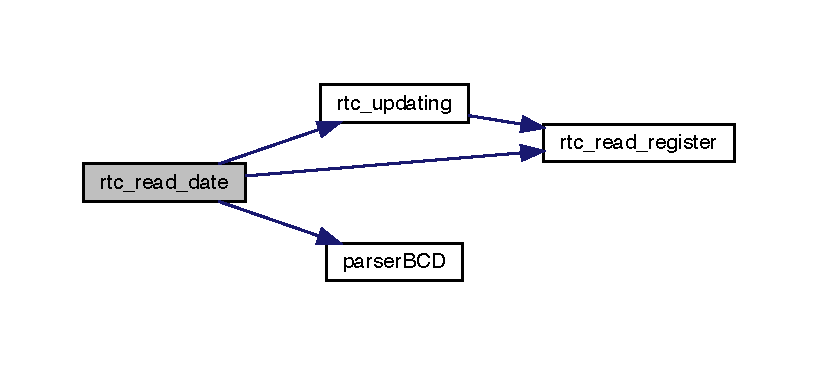
\includegraphics[width=350pt]{group___serial_ga08a02c163edf9dc74b2d15dfb23a2624_cgraph}
\end{center}
\end{figure}
\hypertarget{group___serial_ga50431f28993883d49a09ce054bd5c0ec}{}\label{group___serial_ga50431f28993883d49a09ce054bd5c0ec} 
\index{Port@{Port}!rtc\+\_\+read\+\_\+register@{rtc\+\_\+read\+\_\+register}}
\index{rtc\+\_\+read\+\_\+register@{rtc\+\_\+read\+\_\+register}!Port@{Port}}
\subsubsection{\texorpdfstring{rtc\+\_\+read\+\_\+register()}{rtc\_read\_register()}}
{\footnotesize\ttfamily int rtc\+\_\+read\+\_\+register (\begin{DoxyParamCaption}\item[{int}]{reg }\end{DoxyParamCaption})}



(From Assembly) Reads Value from register reg 


\begin{DoxyParams}{Parameters}
{\em Register} & that will be read\\
\hline
\end{DoxyParams}
\begin{DoxyReturn}{Returns}
Returns bit order in interrupt mask; negative value on failure 
\end{DoxyReturn}
\hypertarget{group___serial_ga6bd13bd1e0cd043f50abb97bcc138bfa}{}\label{group___serial_ga6bd13bd1e0cd043f50abb97bcc138bfa} 
\index{Port@{Port}!rtc\+\_\+subscribe\+\_\+int@{rtc\+\_\+subscribe\+\_\+int}}
\index{rtc\+\_\+subscribe\+\_\+int@{rtc\+\_\+subscribe\+\_\+int}!Port@{Port}}
\subsubsection{\texorpdfstring{rtc\+\_\+subscribe\+\_\+int()}{rtc\_subscribe\_int()}}
{\footnotesize\ttfamily int rtc\+\_\+subscribe\+\_\+int (\begin{DoxyParamCaption}\item[{void}]{ }\end{DoxyParamCaption})}



Subscribes and enables R\+TC interrupts. 

\begin{DoxyReturn}{Returns}
Returns bit order in interrupt mask; negative value on failure 
\end{DoxyReturn}
\hypertarget{group___serial_ga5b1cba4be2c15183b9f2c089fe6e946a}{}\label{group___serial_ga5b1cba4be2c15183b9f2c089fe6e946a} 
\index{Port@{Port}!rtc\+\_\+unsubscribe\+\_\+int@{rtc\+\_\+unsubscribe\+\_\+int}}
\index{rtc\+\_\+unsubscribe\+\_\+int@{rtc\+\_\+unsubscribe\+\_\+int}!Port@{Port}}
\subsubsection{\texorpdfstring{rtc\+\_\+unsubscribe\+\_\+int()}{rtc\_unsubscribe\_int()}}
{\footnotesize\ttfamily int rtc\+\_\+unsubscribe\+\_\+int (\begin{DoxyParamCaption}\item[{void}]{ }\end{DoxyParamCaption})}



Unsubscribes R\+TC interrupts. 

\begin{DoxyReturn}{Returns}
Return 0 upon success and non-\/zero otherwise 
\end{DoxyReturn}
\hypertarget{group___serial_gacaae78073772a1f95560e42cef087a93}{}\label{group___serial_gacaae78073772a1f95560e42cef087a93} 
\index{Port@{Port}!rtc\+\_\+updating@{rtc\+\_\+updating}}
\index{rtc\+\_\+updating@{rtc\+\_\+updating}!Port@{Port}}
\subsubsection{\texorpdfstring{rtc\+\_\+updating()}{rtc\_updating()}}
{\footnotesize\ttfamily int rtc\+\_\+updating (\begin{DoxyParamCaption}\item[{void}]{ }\end{DoxyParamCaption})}

Here is the call graph for this function\+:\nopagebreak
\begin{figure}[H]
\begin{center}
\leavevmode
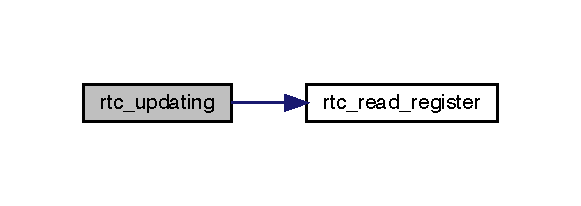
\includegraphics[width=279pt]{group___serial_gacaae78073772a1f95560e42cef087a93_cgraph}
\end{center}
\end{figure}
\hypertarget{group___serial_gab88c07eaefdae0ccbae9e7c2a1e04f71}{}\label{group___serial_gab88c07eaefdae0ccbae9e7c2a1e04f71} 
\index{Port@{Port}!rtc\+\_\+write\+\_\+register@{rtc\+\_\+write\+\_\+register}}
\index{rtc\+\_\+write\+\_\+register@{rtc\+\_\+write\+\_\+register}!Port@{Port}}
\subsubsection{\texorpdfstring{rtc\+\_\+write\+\_\+register()}{rtc\_write\_register()}}
{\footnotesize\ttfamily int rtc\+\_\+write\+\_\+register (\begin{DoxyParamCaption}\item[{unsigned long}]{reg,  }\item[{unsigned long}]{value }\end{DoxyParamCaption})}



Writes value to register reg. 


\begin{DoxyParams}{Parameters}
{\em Register} & to be written\\
\hline
\end{DoxyParams}
New value of register reg

\begin{DoxyReturn}{Returns}
Return 0 upon success and non-\/zero otherwise 
\end{DoxyReturn}
\hypertarget{group___serial_gab84b5f47451f228a5c574b77e5c7e9eb}{}\label{group___serial_gab84b5f47451f228a5c574b77e5c7e9eb} 
\index{Port@{Port}!serial\+\_\+disable\+\_\+interrupts@{serial\+\_\+disable\+\_\+interrupts}}
\index{serial\+\_\+disable\+\_\+interrupts@{serial\+\_\+disable\+\_\+interrupts}!Port@{Port}}
\subsubsection{\texorpdfstring{serial\+\_\+disable\+\_\+interrupts()}{serial\_disable\_interrupts()}}
{\footnotesize\ttfamily int serial\+\_\+disable\+\_\+interrupts (\begin{DoxyParamCaption}{ }\end{DoxyParamCaption})}



Disables Interruptions in the Serial Port. 

\begin{DoxyReturn}{Returns}
Return 0 upon success and non-\/zero otherwise 
\end{DoxyReturn}
\hypertarget{group___serial_ga06724a3064e96e445257aba1e4f3de46}{}\label{group___serial_ga06724a3064e96e445257aba1e4f3de46} 
\index{Port@{Port}!serial\+\_\+enable\+\_\+interrupts@{serial\+\_\+enable\+\_\+interrupts}}
\index{serial\+\_\+enable\+\_\+interrupts@{serial\+\_\+enable\+\_\+interrupts}!Port@{Port}}
\subsubsection{\texorpdfstring{serial\+\_\+enable\+\_\+interrupts()}{serial\_enable\_interrupts()}}
{\footnotesize\ttfamily int serial\+\_\+enable\+\_\+interrupts (\begin{DoxyParamCaption}{ }\end{DoxyParamCaption})}



Enables Interrupt Mode for the Serial Port. 

\begin{DoxyReturn}{Returns}
Return 0 upon success and non-\/zero otherwise
\end{DoxyReturn}
\char`\"{}\+The use of bits 0 and 1 should be obvious\+: if set, the U\+A\+R\+T will generate an interrupt whenever
a character is received and whenever it is ready to accept a new character for transmission, respectively.\char`\"{} \hypertarget{group___serial_ga733df3cf88f5c81a1c4ae2822342dd2d}{}\label{group___serial_ga733df3cf88f5c81a1c4ae2822342dd2d} 
\index{Port@{Port}!serial\+\_\+read@{serial\+\_\+read}}
\index{serial\+\_\+read@{serial\+\_\+read}!Port@{Port}}
\subsubsection{\texorpdfstring{serial\+\_\+read()}{serial\_read()}}
{\footnotesize\ttfamily unsigned char serial\+\_\+read (\begin{DoxyParamCaption}{ }\end{DoxyParamCaption})}



Reads information received using the serial port. 

\begin{DoxyReturn}{Returns}
unsigned char read from the Receiver Buffer 
\end{DoxyReturn}
\hypertarget{group___serial_ga78786e639e5d536f1c65170e7396fde6}{}\label{group___serial_ga78786e639e5d536f1c65170e7396fde6} 
\index{Port@{Port}!serial\+\_\+set\+\_\+conf@{serial\+\_\+set\+\_\+conf}}
\index{serial\+\_\+set\+\_\+conf@{serial\+\_\+set\+\_\+conf}!Port@{Port}}
\subsubsection{\texorpdfstring{serial\+\_\+set\+\_\+conf()}{serial\_set\_conf()}}
{\footnotesize\ttfamily int serial\+\_\+set\+\_\+conf (\begin{DoxyParamCaption}{ }\end{DoxyParamCaption})}



Sets the desired configuration of the U\+A\+RT registers. 

This function should be called in both serial port ends, and any transmission of information

\begin{DoxyReturn}{Returns}
Return 0 upon success and non-\/zero otherwise
\end{DoxyReturn}
" (..)both ends of the serial line must agree on the communication parameters. In the case of asynchronous communication these include the bit rate, the number of bits per character, the number of stop bits and the parity. \hypertarget{group___serial_ga31328528e82730ef05d9e6121447dd42}{}\label{group___serial_ga31328528e82730ef05d9e6121447dd42} 
\index{Port@{Port}!serial\+\_\+subscribe\+\_\+int@{serial\+\_\+subscribe\+\_\+int}}
\index{serial\+\_\+subscribe\+\_\+int@{serial\+\_\+subscribe\+\_\+int}!Port@{Port}}
\subsubsection{\texorpdfstring{serial\+\_\+subscribe\+\_\+int()}{serial\_subscribe\_int()}}
{\footnotesize\ttfamily int serial\+\_\+subscribe\+\_\+int (\begin{DoxyParamCaption}\item[{void}]{ }\end{DoxyParamCaption})}



Subscribes and enables Serial Port interrupts. 

\begin{DoxyReturn}{Returns}
Returns bit order in interrupt mask; negative value on failure 
\end{DoxyReturn}
\hypertarget{group___serial_ga56e227db9f0a79bfb5fd8a753d1be67a}{}\label{group___serial_ga56e227db9f0a79bfb5fd8a753d1be67a} 
\index{Port@{Port}!serial\+\_\+unsubscribe\+\_\+int@{serial\+\_\+unsubscribe\+\_\+int}}
\index{serial\+\_\+unsubscribe\+\_\+int@{serial\+\_\+unsubscribe\+\_\+int}!Port@{Port}}
\subsubsection{\texorpdfstring{serial\+\_\+unsubscribe\+\_\+int()}{serial\_unsubscribe\_int()}}
{\footnotesize\ttfamily int serial\+\_\+unsubscribe\+\_\+int (\begin{DoxyParamCaption}\item[{void}]{ }\end{DoxyParamCaption})}



Unsubscribes Serial Port interrupts. 

\begin{DoxyReturn}{Returns}
Return 0 upon success and non-\/zero otherwise 
\end{DoxyReturn}
\hypertarget{group___serial_ga62f6ef11a701d503d1ed5f4a873a1d2b}{}\label{group___serial_ga62f6ef11a701d503d1ed5f4a873a1d2b} 
\index{Port@{Port}!serial\+\_\+write@{serial\+\_\+write}}
\index{serial\+\_\+write@{serial\+\_\+write}!Port@{Port}}
\subsubsection{\texorpdfstring{serial\+\_\+write()}{serial\_write()}}
{\footnotesize\ttfamily int serial\+\_\+write (\begin{DoxyParamCaption}\item[{unsigned char}]{info }\end{DoxyParamCaption})}



Sends information using the serial port. 


\begin{DoxyParams}{Parameters}
{\em info} & information going to be send\\
\hline
\end{DoxyParams}
\begin{DoxyReturn}{Returns}
Return 0 upon success and non-\/zero otherwise 
\end{DoxyReturn}

\hypertarget{group__timer}{}\section{timer}
\label{group__timer}\index{timer@{timer}}
\subsection*{Functions}
\begin{DoxyCompactItemize}
\item 
int \hyperlink{group__timer_ga7487d2df58374e7945748561966a03fb}{timer\+\_\+delay} (unsigned int t)
\begin{DoxyCompactList}\small\item\em Sleeps for t seconds. \end{DoxyCompactList}\item 
int \hyperlink{group__timer_gada4efbb5c88275795526fc45f0814aa3}{timer\+\_\+set\+\_\+square} (unsigned long timer, unsigned long freq)
\begin{DoxyCompactList}\small\item\em Configures a timer to generate a square wave. \end{DoxyCompactList}\item 
int \hyperlink{group__timer_ga4c5d9f47323eda494cfd826f6d62eec9}{timer\+\_\+subscribe\+\_\+int} (void)
\begin{DoxyCompactList}\small\item\em Subscribes and enables Timer 0 interrupts. \end{DoxyCompactList}\item 
int \hyperlink{group__timer_gab9eea51549744bca5c5c923b388bb4ee}{timer\+\_\+unsubscribe\+\_\+int} ()
\begin{DoxyCompactList}\small\item\em Unsubscribes Timer 0 interrupts. \end{DoxyCompactList}\item 
int \hyperlink{group__timer_ga8eb3357bc05265afc4bea5bbbb480a53}{timer\+\_\+get\+\_\+conf} (unsigned long timer, unsigned char $\ast$st)
\begin{DoxyCompactList}\small\item\em Reads the input timer configuration via read-\/back command. \end{DoxyCompactList}\item 
int \hyperlink{group__timer_ga2e596aede5a7bfc4a6f4382779bf0d7d}{timer\+\_\+test\+\_\+square} (unsigned long freq)
\begin{DoxyCompactList}\small\item\em Tests programming timer in square wave mode. \end{DoxyCompactList}\item 
int \hyperlink{group__timer_ga363e72d1c055d859746cb3305a68af6d}{timer\+\_\+test\+\_\+config} (unsigned long timer)
\begin{DoxyCompactList}\small\item\em Tests display of timer config. \end{DoxyCompactList}\end{DoxyCompactItemize}


\subsection{Detailed Description}
Functions for using the i8254 timers 

\subsection{Function Documentation}
\hypertarget{group__timer_ga7487d2df58374e7945748561966a03fb}{}\label{group__timer_ga7487d2df58374e7945748561966a03fb} 
\index{timer@{timer}!timer\+\_\+delay@{timer\+\_\+delay}}
\index{timer\+\_\+delay@{timer\+\_\+delay}!timer@{timer}}
\subsubsection{\texorpdfstring{timer\+\_\+delay()}{timer\_delay()}}
{\footnotesize\ttfamily int timer\+\_\+delay (\begin{DoxyParamCaption}\item[{unsigned int}]{t }\end{DoxyParamCaption})}



Sleeps for t seconds. 

Uses Timer0

\begin{DoxyReturn}{Returns}
Return 0 upon success and non-\/zero otherwise 
\end{DoxyReturn}
Here is the call graph for this function\+:\nopagebreak
\begin{figure}[H]
\begin{center}
\leavevmode
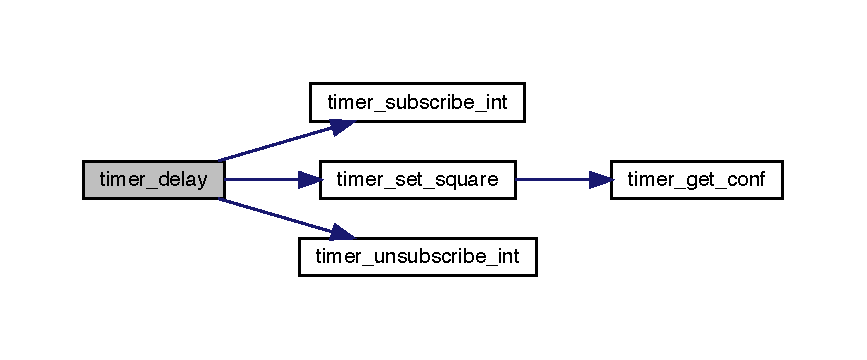
\includegraphics[width=350pt]{group__timer_ga7487d2df58374e7945748561966a03fb_cgraph}
\end{center}
\end{figure}
\hypertarget{group__timer_ga8eb3357bc05265afc4bea5bbbb480a53}{}\label{group__timer_ga8eb3357bc05265afc4bea5bbbb480a53} 
\index{timer@{timer}!timer\+\_\+get\+\_\+conf@{timer\+\_\+get\+\_\+conf}}
\index{timer\+\_\+get\+\_\+conf@{timer\+\_\+get\+\_\+conf}!timer@{timer}}
\subsubsection{\texorpdfstring{timer\+\_\+get\+\_\+conf()}{timer\_get\_conf()}}
{\footnotesize\ttfamily int timer\+\_\+get\+\_\+conf (\begin{DoxyParamCaption}\item[{unsigned long}]{timer,  }\item[{unsigned char $\ast$}]{st }\end{DoxyParamCaption})}



Reads the input timer configuration via read-\/back command. 


\begin{DoxyParams}{Parameters}
{\em timer} & Timer whose config to read (Ranges from 0 to 2) \\
\hline
{\em st} & Address of memory position to be filled with the timer config \\
\hline
\end{DoxyParams}
\begin{DoxyReturn}{Returns}
Return 0 upon success and non-\/zero otherwise 
\end{DoxyReturn}
\hypertarget{group__timer_gada4efbb5c88275795526fc45f0814aa3}{}\label{group__timer_gada4efbb5c88275795526fc45f0814aa3} 
\index{timer@{timer}!timer\+\_\+set\+\_\+square@{timer\+\_\+set\+\_\+square}}
\index{timer\+\_\+set\+\_\+square@{timer\+\_\+set\+\_\+square}!timer@{timer}}
\subsubsection{\texorpdfstring{timer\+\_\+set\+\_\+square()}{timer\_set\_square()}}
{\footnotesize\ttfamily int timer\+\_\+set\+\_\+square (\begin{DoxyParamCaption}\item[{unsigned long}]{timer,  }\item[{unsigned long}]{freq }\end{DoxyParamCaption})}



Configures a timer to generate a square wave. 

Does not change the L\+SB (B\+C\+D/binary) of the timer\textquotesingle{}s control word.


\begin{DoxyParams}{Parameters}
{\em timer} & Timer to configure. (Ranges from 0 to 2) \\
\hline
{\em freq} & Frequency of the square wave to generate \\
\hline
\end{DoxyParams}
\begin{DoxyReturn}{Returns}
Return 0 upon success and non-\/zero otherwise 
\end{DoxyReturn}
Here is the call graph for this function\+:\nopagebreak
\begin{figure}[H]
\begin{center}
\leavevmode
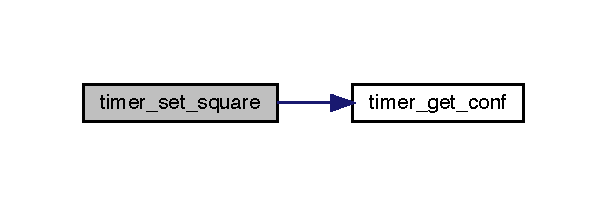
\includegraphics[width=291pt]{group__timer_gada4efbb5c88275795526fc45f0814aa3_cgraph}
\end{center}
\end{figure}
\hypertarget{group__timer_ga4c5d9f47323eda494cfd826f6d62eec9}{}\label{group__timer_ga4c5d9f47323eda494cfd826f6d62eec9} 
\index{timer@{timer}!timer\+\_\+subscribe\+\_\+int@{timer\+\_\+subscribe\+\_\+int}}
\index{timer\+\_\+subscribe\+\_\+int@{timer\+\_\+subscribe\+\_\+int}!timer@{timer}}
\subsubsection{\texorpdfstring{timer\+\_\+subscribe\+\_\+int()}{timer\_subscribe\_int()}}
{\footnotesize\ttfamily int timer\+\_\+subscribe\+\_\+int (\begin{DoxyParamCaption}\item[{void}]{ }\end{DoxyParamCaption})}



Subscribes and enables Timer 0 interrupts. 

\begin{DoxyReturn}{Returns}
Returns bit order in interrupt mask; negative value on failure 
\end{DoxyReturn}
\hypertarget{group__timer_ga363e72d1c055d859746cb3305a68af6d}{}\label{group__timer_ga363e72d1c055d859746cb3305a68af6d} 
\index{timer@{timer}!timer\+\_\+test\+\_\+config@{timer\+\_\+test\+\_\+config}}
\index{timer\+\_\+test\+\_\+config@{timer\+\_\+test\+\_\+config}!timer@{timer}}
\subsubsection{\texorpdfstring{timer\+\_\+test\+\_\+config()}{timer\_test\_config()}}
{\footnotesize\ttfamily int timer\+\_\+test\+\_\+config (\begin{DoxyParamCaption}\item[{unsigned long}]{timer }\end{DoxyParamCaption})}



Tests display of timer config. 

Just calls \hyperlink{group__timer_ga8eb3357bc05265afc4bea5bbbb480a53}{timer\+\_\+get\+\_\+conf()} followed by timer\+\_\+display\+\_\+conf()


\begin{DoxyParams}{Parameters}
{\em timer} & Timer whose config to read (Ranges from 0 to 2) \\
\hline
\end{DoxyParams}
\begin{DoxyReturn}{Returns}
Return 0 upon success and non-\/zero otherwise 
\end{DoxyReturn}
\hypertarget{group__timer_ga2e596aede5a7bfc4a6f4382779bf0d7d}{}\label{group__timer_ga2e596aede5a7bfc4a6f4382779bf0d7d} 
\index{timer@{timer}!timer\+\_\+test\+\_\+square@{timer\+\_\+test\+\_\+square}}
\index{timer\+\_\+test\+\_\+square@{timer\+\_\+test\+\_\+square}!timer@{timer}}
\subsubsection{\texorpdfstring{timer\+\_\+test\+\_\+square()}{timer\_test\_square()}}
{\footnotesize\ttfamily int timer\+\_\+test\+\_\+square (\begin{DoxyParamCaption}\item[{unsigned long}]{freq }\end{DoxyParamCaption})}



Tests programming timer in square wave mode. 

Programs Timer 0 to generate square mode with input frequency


\begin{DoxyParams}{Parameters}
{\em freq} & Frequency of square wave to generate \\
\hline
\end{DoxyParams}
\begin{DoxyReturn}{Returns}
Return 0 upon success and non-\/zero otherwise 
\end{DoxyReturn}
Here is the call graph for this function\+:\nopagebreak
\begin{figure}[H]
\begin{center}
\leavevmode
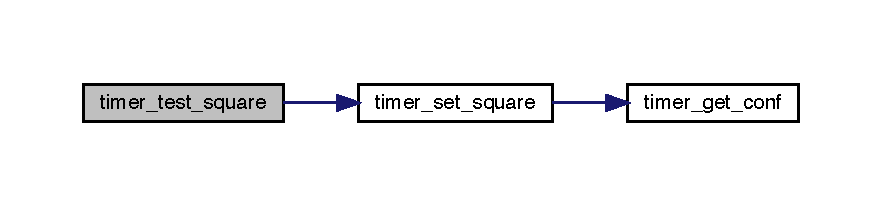
\includegraphics[width=350pt]{group__timer_ga2e596aede5a7bfc4a6f4382779bf0d7d_cgraph}
\end{center}
\end{figure}
\hypertarget{group__timer_gab9eea51549744bca5c5c923b388bb4ee}{}\label{group__timer_gab9eea51549744bca5c5c923b388bb4ee} 
\index{timer@{timer}!timer\+\_\+unsubscribe\+\_\+int@{timer\+\_\+unsubscribe\+\_\+int}}
\index{timer\+\_\+unsubscribe\+\_\+int@{timer\+\_\+unsubscribe\+\_\+int}!timer@{timer}}
\subsubsection{\texorpdfstring{timer\+\_\+unsubscribe\+\_\+int()}{timer\_unsubscribe\_int()}}
{\footnotesize\ttfamily int timer\+\_\+unsubscribe\+\_\+int (\begin{DoxyParamCaption}{ }\end{DoxyParamCaption})}



Unsubscribes Timer 0 interrupts. 

\begin{DoxyReturn}{Returns}
Return 0 upon success and non-\/zero otherwise 
\end{DoxyReturn}

\hypertarget{group__vbe}{}\section{vbe}
\label{group__vbe}\index{vbe@{vbe}}
\subsection*{Classes}
\begin{DoxyCompactItemize}
\item 
struct \hyperlink{struct____attribute____}{\+\_\+\+\_\+attribute\+\_\+\+\_\+}
\end{DoxyCompactItemize}
\subsection*{Macros}
\begin{DoxyCompactItemize}
\item 
\#define \hyperlink{group__vbe_gaf81534a9db918a753a9896b07317b05a}{M\+O\+D\+E\+\_\+800\+X600\+\_\+256}~0\+X103
\item 
\#define \hyperlink{group__vbe_ga22528d5b4d6e5545c28def27f6074fe3}{M\+O\+D\+E\+\_\+1024\+X768\+\_\+256}~0\+X105
\item 
\#define \hyperlink{group__vbe_gafe1e2b1f8808d2531aabf6b94b9947ca}{M\+O\+D\+E\+\_\+1280\+X1024\+\_\+256}~0\+X107
\item 
\#define \hyperlink{group__vbe_gad5df9a29ede26cb662f094f3315de162}{M\+O\+D\+E\+\_\+800\+X600\+\_\+64k}~0\+X114
\end{DoxyCompactItemize}
\subsection*{Functions}
\begin{DoxyCompactItemize}
\item 
int \hyperlink{group__vbe_ga4ef3234e41f2050bc094a22049b69e45}{vbe\+\_\+get\+\_\+mode\+\_\+info} (unsigned short mode, vbe\+\_\+mode\+\_\+info\+\_\+t $\ast$vmi\+\_\+p)
\begin{DoxyCompactList}\small\item\em Returns information on the input V\+BE mode, including screen dimensions, color depth and V\+R\+AM physical address. \end{DoxyCompactList}\item 
void $\ast$ \hyperlink{group__vbe_ga802bfdaa0b951c9fc68eff68d1b27436}{vbe\+\_\+get\+\_\+controller\+\_\+info} (vbe\+\_\+info\+\_\+block $\ast$vbe\+\_\+info\+\_\+p)
\begin{DoxyCompactList}\small\item\em Returns information on the V\+BE controller. \end{DoxyCompactList}\item 
int \hyperlink{group__vbe_ga71fc62857544124047314f3142672cfc}{vbe\+\_\+assert\+\_\+error} (unsigned char e)
\begin{DoxyCompactList}\small\item\em Asserts whether the V\+BE byte response indicates an error, and prints accordingly. \end{DoxyCompactList}\end{DoxyCompactItemize}
\subsection*{V\+BE Functions}
\begin{DoxyCompactItemize}
\item 
\#define \hyperlink{group__vbe_ga13e1037464e7407d1df6aa4041b180cd}{V\+B\+E\+\_\+\+I\+N\+T\+E\+R\+R\+U\+PT}~0x10
\item 
\#define \hyperlink{group__vbe_gaaa7fbe1e02a424af8eb9efc320d936c0}{V\+B\+E\+\_\+\+C\+A\+LL}~0x4F
\item 
\#define \hyperlink{group__vbe_gacbb1e5e9b91d58f76eb6c0554f03fc8c}{G\+E\+T\+\_\+\+V\+B\+E\+\_\+\+C\+O\+N\+T\+R\+O\+L\+L\+E\+R\+\_\+\+I\+N\+FO}~0x00
\item 
\#define \hyperlink{group__vbe_gac3faf02beab492e13687e9f10efb6ca4}{G\+E\+T\+\_\+\+V\+B\+E\+\_\+\+M\+O\+D\+E\+\_\+\+I\+N\+FO}~0x01
\item 
\#define \hyperlink{group__vbe_gab32156e1d72cb92b120bb16883c87eea}{S\+E\+T\+\_\+\+V\+B\+E\+\_\+\+M\+O\+DE}~0x02
\item 
\#define \hyperlink{group__vbe_ga64d38e10ac1b86615156b96e82b82ebc}{G\+E\+T\+\_\+\+C\+U\+R\+R\+E\+N\+T\+\_\+\+V\+B\+E\+\_\+\+M\+O\+DE}~0x03
\item 
\#define \hyperlink{group__vbe_ga87cd9f2b19724f7bef3327973717eee4}{S\+A\+V\+E\+\_\+\+R\+E\+S\+T\+O\+R\+E\+\_\+\+S\+T\+A\+TE}~0x04
\item 
\#define \hyperlink{group__vbe_gaaa8c204b50ef83c6d2819bf00a254c84}{D\+I\+S\+P\+L\+A\+Y\+\_\+\+W\+I\+N\+D\+O\+W\+\_\+\+C\+O\+N\+T\+R\+OL}~0x05
\item 
\#define \hyperlink{group__vbe_ga4db24dade600a2ae03a6c85121f932eb}{S\+E\+T\+\_\+\+G\+E\+T\+\_\+\+S\+C\+A\+N\+\_\+\+L\+E\+N\+G\+TH}~0x06
\item 
\#define \hyperlink{group__vbe_ga08e732a570bdadf08bac384db646be8a}{S\+E\+T\+\_\+\+G\+E\+T\+\_\+\+D\+I\+S\+P\+L\+A\+Y\+\_\+\+S\+T\+A\+RT}~0x07
\item 
\#define \hyperlink{group__vbe_gaef71e0667c3e5dbc58fa9b150b8a077a}{S\+E\+T\+\_\+\+G\+E\+T\+\_\+\+P\+A\+L\+E\+T\+T\+E\+\_\+\+F\+O\+R\+M\+AT}~0x08
\item 
\#define \hyperlink{group__vbe_ga7fd3951844513e578e8a93ca8ef7b39d}{S\+E\+T\+\_\+\+G\+E\+T\+\_\+\+P\+A\+L\+E\+T\+T\+E\+\_\+\+D\+A\+TA}~0x09
\item 
\#define \hyperlink{group__vbe_ga78c6b278f083525b36116e11a86e05b3}{G\+E\+T\+\_\+\+P\+T\+R\+\_\+\+P\+R\+O\+T\+E\+C\+T\+ED}
\end{DoxyCompactItemize}


\subsection{Detailed Description}
Functions related to the V\+BE standard 

\subsection{Macro Definition Documentation}
\hypertarget{group__vbe_gaaa8c204b50ef83c6d2819bf00a254c84}{}\label{group__vbe_gaaa8c204b50ef83c6d2819bf00a254c84} 
\index{vbe@{vbe}!D\+I\+S\+P\+L\+A\+Y\+\_\+\+W\+I\+N\+D\+O\+W\+\_\+\+C\+O\+N\+T\+R\+OL@{D\+I\+S\+P\+L\+A\+Y\+\_\+\+W\+I\+N\+D\+O\+W\+\_\+\+C\+O\+N\+T\+R\+OL}}
\index{D\+I\+S\+P\+L\+A\+Y\+\_\+\+W\+I\+N\+D\+O\+W\+\_\+\+C\+O\+N\+T\+R\+OL@{D\+I\+S\+P\+L\+A\+Y\+\_\+\+W\+I\+N\+D\+O\+W\+\_\+\+C\+O\+N\+T\+R\+OL}!vbe@{vbe}}
\subsubsection{\texorpdfstring{D\+I\+S\+P\+L\+A\+Y\+\_\+\+W\+I\+N\+D\+O\+W\+\_\+\+C\+O\+N\+T\+R\+OL}{DISPLAY\_WINDOW\_CONTROL}}
{\footnotesize\ttfamily \#define D\+I\+S\+P\+L\+A\+Y\+\_\+\+W\+I\+N\+D\+O\+W\+\_\+\+C\+O\+N\+T\+R\+OL~0x05}

\hypertarget{group__vbe_ga64d38e10ac1b86615156b96e82b82ebc}{}\label{group__vbe_ga64d38e10ac1b86615156b96e82b82ebc} 
\index{vbe@{vbe}!G\+E\+T\+\_\+\+C\+U\+R\+R\+E\+N\+T\+\_\+\+V\+B\+E\+\_\+\+M\+O\+DE@{G\+E\+T\+\_\+\+C\+U\+R\+R\+E\+N\+T\+\_\+\+V\+B\+E\+\_\+\+M\+O\+DE}}
\index{G\+E\+T\+\_\+\+C\+U\+R\+R\+E\+N\+T\+\_\+\+V\+B\+E\+\_\+\+M\+O\+DE@{G\+E\+T\+\_\+\+C\+U\+R\+R\+E\+N\+T\+\_\+\+V\+B\+E\+\_\+\+M\+O\+DE}!vbe@{vbe}}
\subsubsection{\texorpdfstring{G\+E\+T\+\_\+\+C\+U\+R\+R\+E\+N\+T\+\_\+\+V\+B\+E\+\_\+\+M\+O\+DE}{GET\_CURRENT\_VBE\_MODE}}
{\footnotesize\ttfamily \#define G\+E\+T\+\_\+\+C\+U\+R\+R\+E\+N\+T\+\_\+\+V\+B\+E\+\_\+\+M\+O\+DE~0x03}

\hypertarget{group__vbe_ga78c6b278f083525b36116e11a86e05b3}{}\label{group__vbe_ga78c6b278f083525b36116e11a86e05b3} 
\index{vbe@{vbe}!G\+E\+T\+\_\+\+P\+T\+R\+\_\+\+P\+R\+O\+T\+E\+C\+T\+ED@{G\+E\+T\+\_\+\+P\+T\+R\+\_\+\+P\+R\+O\+T\+E\+C\+T\+ED}}
\index{G\+E\+T\+\_\+\+P\+T\+R\+\_\+\+P\+R\+O\+T\+E\+C\+T\+ED@{G\+E\+T\+\_\+\+P\+T\+R\+\_\+\+P\+R\+O\+T\+E\+C\+T\+ED}!vbe@{vbe}}
\subsubsection{\texorpdfstring{G\+E\+T\+\_\+\+P\+T\+R\+\_\+\+P\+R\+O\+T\+E\+C\+T\+ED}{GET\_PTR\_PROTECTED}}
{\footnotesize\ttfamily \#define G\+E\+T\+\_\+\+P\+T\+R\+\_\+\+P\+R\+O\+T\+E\+C\+T\+ED}

\hypertarget{group__vbe_gacbb1e5e9b91d58f76eb6c0554f03fc8c}{}\label{group__vbe_gacbb1e5e9b91d58f76eb6c0554f03fc8c} 
\index{vbe@{vbe}!G\+E\+T\+\_\+\+V\+B\+E\+\_\+\+C\+O\+N\+T\+R\+O\+L\+L\+E\+R\+\_\+\+I\+N\+FO@{G\+E\+T\+\_\+\+V\+B\+E\+\_\+\+C\+O\+N\+T\+R\+O\+L\+L\+E\+R\+\_\+\+I\+N\+FO}}
\index{G\+E\+T\+\_\+\+V\+B\+E\+\_\+\+C\+O\+N\+T\+R\+O\+L\+L\+E\+R\+\_\+\+I\+N\+FO@{G\+E\+T\+\_\+\+V\+B\+E\+\_\+\+C\+O\+N\+T\+R\+O\+L\+L\+E\+R\+\_\+\+I\+N\+FO}!vbe@{vbe}}
\subsubsection{\texorpdfstring{G\+E\+T\+\_\+\+V\+B\+E\+\_\+\+C\+O\+N\+T\+R\+O\+L\+L\+E\+R\+\_\+\+I\+N\+FO}{GET\_VBE\_CONTROLLER\_INFO}}
{\footnotesize\ttfamily \#define G\+E\+T\+\_\+\+V\+B\+E\+\_\+\+C\+O\+N\+T\+R\+O\+L\+L\+E\+R\+\_\+\+I\+N\+FO~0x00}

\hypertarget{group__vbe_gac3faf02beab492e13687e9f10efb6ca4}{}\label{group__vbe_gac3faf02beab492e13687e9f10efb6ca4} 
\index{vbe@{vbe}!G\+E\+T\+\_\+\+V\+B\+E\+\_\+\+M\+O\+D\+E\+\_\+\+I\+N\+FO@{G\+E\+T\+\_\+\+V\+B\+E\+\_\+\+M\+O\+D\+E\+\_\+\+I\+N\+FO}}
\index{G\+E\+T\+\_\+\+V\+B\+E\+\_\+\+M\+O\+D\+E\+\_\+\+I\+N\+FO@{G\+E\+T\+\_\+\+V\+B\+E\+\_\+\+M\+O\+D\+E\+\_\+\+I\+N\+FO}!vbe@{vbe}}
\subsubsection{\texorpdfstring{G\+E\+T\+\_\+\+V\+B\+E\+\_\+\+M\+O\+D\+E\+\_\+\+I\+N\+FO}{GET\_VBE\_MODE\_INFO}}
{\footnotesize\ttfamily \#define G\+E\+T\+\_\+\+V\+B\+E\+\_\+\+M\+O\+D\+E\+\_\+\+I\+N\+FO~0x01}

\hypertarget{group__vbe_ga22528d5b4d6e5545c28def27f6074fe3}{}\label{group__vbe_ga22528d5b4d6e5545c28def27f6074fe3} 
\index{vbe@{vbe}!M\+O\+D\+E\+\_\+1024\+X768\+\_\+256@{M\+O\+D\+E\+\_\+1024\+X768\+\_\+256}}
\index{M\+O\+D\+E\+\_\+1024\+X768\+\_\+256@{M\+O\+D\+E\+\_\+1024\+X768\+\_\+256}!vbe@{vbe}}
\subsubsection{\texorpdfstring{M\+O\+D\+E\+\_\+1024\+X768\+\_\+256}{MODE\_1024X768\_256}}
{\footnotesize\ttfamily \#define M\+O\+D\+E\+\_\+1024\+X768\+\_\+256~0\+X105}

\hypertarget{group__vbe_gafe1e2b1f8808d2531aabf6b94b9947ca}{}\label{group__vbe_gafe1e2b1f8808d2531aabf6b94b9947ca} 
\index{vbe@{vbe}!M\+O\+D\+E\+\_\+1280\+X1024\+\_\+256@{M\+O\+D\+E\+\_\+1280\+X1024\+\_\+256}}
\index{M\+O\+D\+E\+\_\+1280\+X1024\+\_\+256@{M\+O\+D\+E\+\_\+1280\+X1024\+\_\+256}!vbe@{vbe}}
\subsubsection{\texorpdfstring{M\+O\+D\+E\+\_\+1280\+X1024\+\_\+256}{MODE\_1280X1024\_256}}
{\footnotesize\ttfamily \#define M\+O\+D\+E\+\_\+1280\+X1024\+\_\+256~0\+X107}

\hypertarget{group__vbe_gaf81534a9db918a753a9896b07317b05a}{}\label{group__vbe_gaf81534a9db918a753a9896b07317b05a} 
\index{vbe@{vbe}!M\+O\+D\+E\+\_\+800\+X600\+\_\+256@{M\+O\+D\+E\+\_\+800\+X600\+\_\+256}}
\index{M\+O\+D\+E\+\_\+800\+X600\+\_\+256@{M\+O\+D\+E\+\_\+800\+X600\+\_\+256}!vbe@{vbe}}
\subsubsection{\texorpdfstring{M\+O\+D\+E\+\_\+800\+X600\+\_\+256}{MODE\_800X600\_256}}
{\footnotesize\ttfamily \#define M\+O\+D\+E\+\_\+800\+X600\+\_\+256~0\+X103}

\hypertarget{group__vbe_gad5df9a29ede26cb662f094f3315de162}{}\label{group__vbe_gad5df9a29ede26cb662f094f3315de162} 
\index{vbe@{vbe}!M\+O\+D\+E\+\_\+800\+X600\+\_\+64k@{M\+O\+D\+E\+\_\+800\+X600\+\_\+64k}}
\index{M\+O\+D\+E\+\_\+800\+X600\+\_\+64k@{M\+O\+D\+E\+\_\+800\+X600\+\_\+64k}!vbe@{vbe}}
\subsubsection{\texorpdfstring{M\+O\+D\+E\+\_\+800\+X600\+\_\+64k}{MODE\_800X600\_64k}}
{\footnotesize\ttfamily \#define M\+O\+D\+E\+\_\+800\+X600\+\_\+64k~0\+X114}

\hypertarget{group__vbe_ga87cd9f2b19724f7bef3327973717eee4}{}\label{group__vbe_ga87cd9f2b19724f7bef3327973717eee4} 
\index{vbe@{vbe}!S\+A\+V\+E\+\_\+\+R\+E\+S\+T\+O\+R\+E\+\_\+\+S\+T\+A\+TE@{S\+A\+V\+E\+\_\+\+R\+E\+S\+T\+O\+R\+E\+\_\+\+S\+T\+A\+TE}}
\index{S\+A\+V\+E\+\_\+\+R\+E\+S\+T\+O\+R\+E\+\_\+\+S\+T\+A\+TE@{S\+A\+V\+E\+\_\+\+R\+E\+S\+T\+O\+R\+E\+\_\+\+S\+T\+A\+TE}!vbe@{vbe}}
\subsubsection{\texorpdfstring{S\+A\+V\+E\+\_\+\+R\+E\+S\+T\+O\+R\+E\+\_\+\+S\+T\+A\+TE}{SAVE\_RESTORE\_STATE}}
{\footnotesize\ttfamily \#define S\+A\+V\+E\+\_\+\+R\+E\+S\+T\+O\+R\+E\+\_\+\+S\+T\+A\+TE~0x04}

\hypertarget{group__vbe_ga08e732a570bdadf08bac384db646be8a}{}\label{group__vbe_ga08e732a570bdadf08bac384db646be8a} 
\index{vbe@{vbe}!S\+E\+T\+\_\+\+G\+E\+T\+\_\+\+D\+I\+S\+P\+L\+A\+Y\+\_\+\+S\+T\+A\+RT@{S\+E\+T\+\_\+\+G\+E\+T\+\_\+\+D\+I\+S\+P\+L\+A\+Y\+\_\+\+S\+T\+A\+RT}}
\index{S\+E\+T\+\_\+\+G\+E\+T\+\_\+\+D\+I\+S\+P\+L\+A\+Y\+\_\+\+S\+T\+A\+RT@{S\+E\+T\+\_\+\+G\+E\+T\+\_\+\+D\+I\+S\+P\+L\+A\+Y\+\_\+\+S\+T\+A\+RT}!vbe@{vbe}}
\subsubsection{\texorpdfstring{S\+E\+T\+\_\+\+G\+E\+T\+\_\+\+D\+I\+S\+P\+L\+A\+Y\+\_\+\+S\+T\+A\+RT}{SET\_GET\_DISPLAY\_START}}
{\footnotesize\ttfamily \#define S\+E\+T\+\_\+\+G\+E\+T\+\_\+\+D\+I\+S\+P\+L\+A\+Y\+\_\+\+S\+T\+A\+RT~0x07}

\hypertarget{group__vbe_ga7fd3951844513e578e8a93ca8ef7b39d}{}\label{group__vbe_ga7fd3951844513e578e8a93ca8ef7b39d} 
\index{vbe@{vbe}!S\+E\+T\+\_\+\+G\+E\+T\+\_\+\+P\+A\+L\+E\+T\+T\+E\+\_\+\+D\+A\+TA@{S\+E\+T\+\_\+\+G\+E\+T\+\_\+\+P\+A\+L\+E\+T\+T\+E\+\_\+\+D\+A\+TA}}
\index{S\+E\+T\+\_\+\+G\+E\+T\+\_\+\+P\+A\+L\+E\+T\+T\+E\+\_\+\+D\+A\+TA@{S\+E\+T\+\_\+\+G\+E\+T\+\_\+\+P\+A\+L\+E\+T\+T\+E\+\_\+\+D\+A\+TA}!vbe@{vbe}}
\subsubsection{\texorpdfstring{S\+E\+T\+\_\+\+G\+E\+T\+\_\+\+P\+A\+L\+E\+T\+T\+E\+\_\+\+D\+A\+TA}{SET\_GET\_PALETTE\_DATA}}
{\footnotesize\ttfamily \#define S\+E\+T\+\_\+\+G\+E\+T\+\_\+\+P\+A\+L\+E\+T\+T\+E\+\_\+\+D\+A\+TA~0x09}

\hypertarget{group__vbe_gaef71e0667c3e5dbc58fa9b150b8a077a}{}\label{group__vbe_gaef71e0667c3e5dbc58fa9b150b8a077a} 
\index{vbe@{vbe}!S\+E\+T\+\_\+\+G\+E\+T\+\_\+\+P\+A\+L\+E\+T\+T\+E\+\_\+\+F\+O\+R\+M\+AT@{S\+E\+T\+\_\+\+G\+E\+T\+\_\+\+P\+A\+L\+E\+T\+T\+E\+\_\+\+F\+O\+R\+M\+AT}}
\index{S\+E\+T\+\_\+\+G\+E\+T\+\_\+\+P\+A\+L\+E\+T\+T\+E\+\_\+\+F\+O\+R\+M\+AT@{S\+E\+T\+\_\+\+G\+E\+T\+\_\+\+P\+A\+L\+E\+T\+T\+E\+\_\+\+F\+O\+R\+M\+AT}!vbe@{vbe}}
\subsubsection{\texorpdfstring{S\+E\+T\+\_\+\+G\+E\+T\+\_\+\+P\+A\+L\+E\+T\+T\+E\+\_\+\+F\+O\+R\+M\+AT}{SET\_GET\_PALETTE\_FORMAT}}
{\footnotesize\ttfamily \#define S\+E\+T\+\_\+\+G\+E\+T\+\_\+\+P\+A\+L\+E\+T\+T\+E\+\_\+\+F\+O\+R\+M\+AT~0x08}

\hypertarget{group__vbe_ga4db24dade600a2ae03a6c85121f932eb}{}\label{group__vbe_ga4db24dade600a2ae03a6c85121f932eb} 
\index{vbe@{vbe}!S\+E\+T\+\_\+\+G\+E\+T\+\_\+\+S\+C\+A\+N\+\_\+\+L\+E\+N\+G\+TH@{S\+E\+T\+\_\+\+G\+E\+T\+\_\+\+S\+C\+A\+N\+\_\+\+L\+E\+N\+G\+TH}}
\index{S\+E\+T\+\_\+\+G\+E\+T\+\_\+\+S\+C\+A\+N\+\_\+\+L\+E\+N\+G\+TH@{S\+E\+T\+\_\+\+G\+E\+T\+\_\+\+S\+C\+A\+N\+\_\+\+L\+E\+N\+G\+TH}!vbe@{vbe}}
\subsubsection{\texorpdfstring{S\+E\+T\+\_\+\+G\+E\+T\+\_\+\+S\+C\+A\+N\+\_\+\+L\+E\+N\+G\+TH}{SET\_GET\_SCAN\_LENGTH}}
{\footnotesize\ttfamily \#define S\+E\+T\+\_\+\+G\+E\+T\+\_\+\+S\+C\+A\+N\+\_\+\+L\+E\+N\+G\+TH~0x06}

\hypertarget{group__vbe_gab32156e1d72cb92b120bb16883c87eea}{}\label{group__vbe_gab32156e1d72cb92b120bb16883c87eea} 
\index{vbe@{vbe}!S\+E\+T\+\_\+\+V\+B\+E\+\_\+\+M\+O\+DE@{S\+E\+T\+\_\+\+V\+B\+E\+\_\+\+M\+O\+DE}}
\index{S\+E\+T\+\_\+\+V\+B\+E\+\_\+\+M\+O\+DE@{S\+E\+T\+\_\+\+V\+B\+E\+\_\+\+M\+O\+DE}!vbe@{vbe}}
\subsubsection{\texorpdfstring{S\+E\+T\+\_\+\+V\+B\+E\+\_\+\+M\+O\+DE}{SET\_VBE\_MODE}}
{\footnotesize\ttfamily \#define S\+E\+T\+\_\+\+V\+B\+E\+\_\+\+M\+O\+DE~0x02}

\hypertarget{group__vbe_gaaa7fbe1e02a424af8eb9efc320d936c0}{}\label{group__vbe_gaaa7fbe1e02a424af8eb9efc320d936c0} 
\index{vbe@{vbe}!V\+B\+E\+\_\+\+C\+A\+LL@{V\+B\+E\+\_\+\+C\+A\+LL}}
\index{V\+B\+E\+\_\+\+C\+A\+LL@{V\+B\+E\+\_\+\+C\+A\+LL}!vbe@{vbe}}
\subsubsection{\texorpdfstring{V\+B\+E\+\_\+\+C\+A\+LL}{VBE\_CALL}}
{\footnotesize\ttfamily \#define V\+B\+E\+\_\+\+C\+A\+LL~0x4F}

\hypertarget{group__vbe_ga13e1037464e7407d1df6aa4041b180cd}{}\label{group__vbe_ga13e1037464e7407d1df6aa4041b180cd} 
\index{vbe@{vbe}!V\+B\+E\+\_\+\+I\+N\+T\+E\+R\+R\+U\+PT@{V\+B\+E\+\_\+\+I\+N\+T\+E\+R\+R\+U\+PT}}
\index{V\+B\+E\+\_\+\+I\+N\+T\+E\+R\+R\+U\+PT@{V\+B\+E\+\_\+\+I\+N\+T\+E\+R\+R\+U\+PT}!vbe@{vbe}}
\subsubsection{\texorpdfstring{V\+B\+E\+\_\+\+I\+N\+T\+E\+R\+R\+U\+PT}{VBE\_INTERRUPT}}
{\footnotesize\ttfamily \#define V\+B\+E\+\_\+\+I\+N\+T\+E\+R\+R\+U\+PT~0x10}

V\+BE Functions from Chapter 4 

\subsection{Function Documentation}
\hypertarget{group__vbe_ga71fc62857544124047314f3142672cfc}{}\label{group__vbe_ga71fc62857544124047314f3142672cfc} 
\index{vbe@{vbe}!vbe\+\_\+assert\+\_\+error@{vbe\+\_\+assert\+\_\+error}}
\index{vbe\+\_\+assert\+\_\+error@{vbe\+\_\+assert\+\_\+error}!vbe@{vbe}}
\subsubsection{\texorpdfstring{vbe\+\_\+assert\+\_\+error()}{vbe\_assert\_error()}}
{\footnotesize\ttfamily int vbe\+\_\+assert\+\_\+error (\begin{DoxyParamCaption}\item[{unsigned char}]{e }\end{DoxyParamCaption})}



Asserts whether the V\+BE byte response indicates an error, and prints accordingly. 


\begin{DoxyParams}{Parameters}
{\em Byte} & returned in the AH\\
\hline
\end{DoxyParams}
\begin{DoxyReturn}{Returns}
0 on success, non-\/zero otherwise 
\end{DoxyReturn}
\hypertarget{group__vbe_ga802bfdaa0b951c9fc68eff68d1b27436}{}\label{group__vbe_ga802bfdaa0b951c9fc68eff68d1b27436} 
\index{vbe@{vbe}!vbe\+\_\+get\+\_\+controller\+\_\+info@{vbe\+\_\+get\+\_\+controller\+\_\+info}}
\index{vbe\+\_\+get\+\_\+controller\+\_\+info@{vbe\+\_\+get\+\_\+controller\+\_\+info}!vbe@{vbe}}
\subsubsection{\texorpdfstring{vbe\+\_\+get\+\_\+controller\+\_\+info()}{vbe\_get\_controller\_info()}}
{\footnotesize\ttfamily void$\ast$ vbe\+\_\+get\+\_\+controller\+\_\+info (\begin{DoxyParamCaption}\item[{vbe\+\_\+info\+\_\+block $\ast$}]{vbe\+\_\+info\+\_\+p }\end{DoxyParamCaption})}



Returns information on the V\+BE controller. 

Initializes unpacked vbe\+\_\+info\+\_\+block structure passed as an address, by calling V\+BE function 0x00. Returns V\+BE Controller Information.


\begin{DoxyParams}{Parameters}
{\em vbe\+\_\+info\+\_\+p} & address of vbe\+\_\+info\+\_\+block structure to be initialized \\
\hline
\end{DoxyParams}
\begin{DoxyReturn}{Returns}
0 on success, non-\/zero otherwise 
\end{DoxyReturn}
Here is the call graph for this function\+:\nopagebreak
\begin{figure}[H]
\begin{center}
\leavevmode
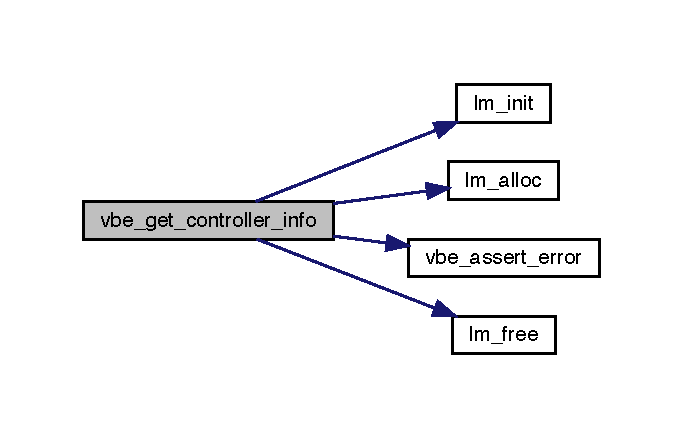
\includegraphics[width=328pt]{group__vbe_ga802bfdaa0b951c9fc68eff68d1b27436_cgraph}
\end{center}
\end{figure}
\hypertarget{group__vbe_ga4ef3234e41f2050bc094a22049b69e45}{}\label{group__vbe_ga4ef3234e41f2050bc094a22049b69e45} 
\index{vbe@{vbe}!vbe\+\_\+get\+\_\+mode\+\_\+info@{vbe\+\_\+get\+\_\+mode\+\_\+info}}
\index{vbe\+\_\+get\+\_\+mode\+\_\+info@{vbe\+\_\+get\+\_\+mode\+\_\+info}!vbe@{vbe}}
\subsubsection{\texorpdfstring{vbe\+\_\+get\+\_\+mode\+\_\+info()}{vbe\_get\_mode\_info()}}
{\footnotesize\ttfamily int vbe\+\_\+get\+\_\+mode\+\_\+info (\begin{DoxyParamCaption}\item[{unsigned short}]{mode,  }\item[{vbe\+\_\+mode\+\_\+info\+\_\+t $\ast$}]{vmi\+\_\+p }\end{DoxyParamCaption})}



Returns information on the input V\+BE mode, including screen dimensions, color depth and V\+R\+AM physical address. 

Initializes unpacked vbe\+\_\+mode\+\_\+\+\_\+info\+\_\+t structure passed as an address with the information of the input mode, by calling V\+BE function 0x01 Return V\+BE Mode Information and unpacking the Mode\+Info\+Block struct returned by that function.


\begin{DoxyParams}{Parameters}
{\em mode} & mode whose information should be returned \\
\hline
{\em vmi\+\_\+p} & address of vbe\+\_\+mode\+\_\+info\+\_\+t structure to be initialized \\
\hline
\end{DoxyParams}
\begin{DoxyReturn}{Returns}
0 on success, non-\/zero otherwise 
\end{DoxyReturn}
Here is the call graph for this function\+:\nopagebreak
\begin{figure}[H]
\begin{center}
\leavevmode
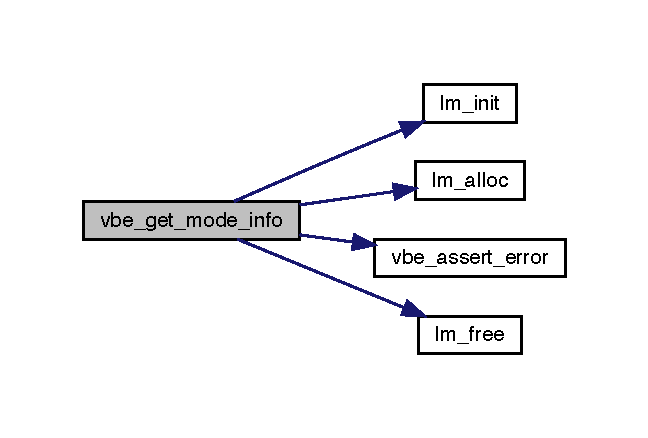
\includegraphics[width=311pt]{group__vbe_ga4ef3234e41f2050bc094a22049b69e45_cgraph}
\end{center}
\end{figure}

\hypertarget{group__video__gr}{}\section{video\+\_\+gr}
\label{group__video__gr}\index{video\+\_\+gr@{video\+\_\+gr}}
\subsection*{Macros}
\begin{DoxyCompactItemize}
\item 
\#define \hyperlink{group__video__gr_ga7b3b25cba33b07c303f3060fe41887f6}{B\+L\+A\+CK}~\hyperlink{group__video__gr_gafcc897567998ed3a26974926501a4abd}{rgb}(0,0,0)
\item 
\#define \hyperlink{group__video__gr_ga87b537f5fa5c109d3c05c13d6b18f382}{W\+H\+I\+TE}~\hyperlink{group__video__gr_gafcc897567998ed3a26974926501a4abd}{rgb}(255,255,255)
\item 
\#define \hyperlink{group__video__gr_gad2cbbe762a1a1175055cf68cd586adc1}{T\+R\+A\+N\+S\+P\+A\+R\+E\+N\+CY}~\hyperlink{group__video__gr_gafcc897567998ed3a26974926501a4abd}{rgb}(0,255,0)
\item 
\#define \hyperlink{group__video__gr_ga1dd918deb1dda207fd2665e93b575e36}{S\+T\+R\+O\+N\+G\+\_\+\+P\+I\+NK}~\hyperlink{group__video__gr_gafcc897567998ed3a26974926501a4abd}{rgb}(255,0,127)
\item 
\#define \hyperlink{group__video__gr_gab2ee9bdede8e3af96ff696c7b2ba7416}{N\+A\+VY}~\hyperlink{group__video__gr_gafcc897567998ed3a26974926501a4abd}{rgb}(0,128,255)
\item 
\#define \hyperlink{group__video__gr_ga8d23feea868a983c8c2b661e1e16972f}{R\+ED}~\hyperlink{group__video__gr_gafcc897567998ed3a26974926501a4abd}{rgb}(255,0,0)
\item 
\#define \hyperlink{group__video__gr_gabf681265909adf3d3e8116c93c0ba179}{Y\+E\+L\+L\+OW}~\hyperlink{group__video__gr_gafcc897567998ed3a26974926501a4abd}{rgb}(255,255,0)
\item 
\#define \hyperlink{group__video__gr_ga6f699060902f800f12aaae150f3a708e}{M\+A\+G\+E\+N\+TA}~\hyperlink{group__video__gr_gafcc897567998ed3a26974926501a4abd}{rgb}(255, 24, 127)
\end{DoxyCompactItemize}
\subsection*{Functions}
\begin{DoxyCompactItemize}
\item 
unsigned \hyperlink{group__video__gr_gab3938dd22c03335341584d5b8f6752f5}{vg\+\_\+get\+Hor\+Res} ()
\begin{DoxyCompactList}\small\item\em Gets the horizontal Resolution of the screen. \end{DoxyCompactList}\item 
unsigned \hyperlink{group__video__gr_gaab8200f7947926322b6dd6fa7c6da1e1}{vg\+\_\+get\+Ver\+Res} ()
\begin{DoxyCompactList}\small\item\em Gets the vertical Resolution of the screen. \end{DoxyCompactList}\item 
void $\ast$ \hyperlink{group__video__gr_gabd51eef0a4ffcafb6a08fb40703f4383}{vg\+\_\+get\+Buffer\+Ptr} ()
\begin{DoxyCompactList}\small\item\em Gets the pointer to the graphics Buffer used for double-\/buffering. \end{DoxyCompactList}\item 
int \hyperlink{group__video__gr_ga7f93731e89220a67419a16b1a415e133}{is\+\_\+valid\+\_\+pos} (unsigned short x, unsigned short y)
\begin{DoxyCompactList}\small\item\em Checks if position (x,y) is inside the screen. \end{DoxyCompactList}\item 
void \hyperlink{group__video__gr_gafd0836c92e142e75c256799fb45032da}{paint\+\_\+pixel} (int x, int y, uint16\+\_\+t color)
\item 
int \hyperlink{group__video__gr_ga7d19c24f10ca7bfb2c7b8f9e12d4dc6f}{vg\+\_\+init} (unsigned short mode)
\begin{DoxyCompactList}\small\item\em Initializes the video module in graphics mode. \end{DoxyCompactList}\item 
int \hyperlink{group__video__gr_ga42f593e6656f1a978315aff02b1bcebf}{vg\+\_\+exit} (void)
\begin{DoxyCompactList}\small\item\em Returns to default Minix 3 text mode (0x03\+: 25 x 80, 16 colors) \end{DoxyCompactList}\item 
int \hyperlink{group__video__gr_ga0b618a385e591f8690388281fd79a351}{draw\+\_\+line} (unsigned short xi, unsigned short yi, unsigned short xf, unsigned short yf, uint16\+\_\+t color)
\begin{DoxyCompactList}\small\item\em Draws a line on the screen, given a color, a initial position and a final position. \end{DoxyCompactList}\item 
int \hyperlink{group__video__gr_ga6494f21641e972c58acdaedcf9c80520}{draw\+\_\+circle} (unsigned short center\+\_\+x, unsigned short center\+\_\+y, unsigned short radius, uint16\+\_\+t color)
\begin{DoxyCompactList}\small\item\em Draws a circle on the screen, given a color, a center position and a radius. \end{DoxyCompactList}\item 
int \hyperlink{group__video__gr_ga5cb0e000108ddc786148172ee56903c3}{draw\+\_\+mouse\+\_\+cross} (const int $\ast$mouse\+\_\+pos, uint16\+\_\+t color)
\begin{DoxyCompactList}\small\item\em Draws the mouse cross at a certain position with a certain color. \end{DoxyCompactList}\item 
void \hyperlink{group__video__gr_ga4270ae09ddc191cdc0e767e4412c386a}{draw\+\_\+missile} (\hyperlink{group___missile_ga7ea98f7c879356e5dfa41934529d86e1}{Missile} $\ast$ptr)
\begin{DoxyCompactList}\small\item\em Draws a missile. \end{DoxyCompactList}\item 
void \hyperlink{group__video__gr_ga8dca584eb65462cd691cb94a9ec92602}{draw\+\_\+number} (unsigned num, \hyperlink{struct_bitmap}{Bitmap} $\ast$$\ast$font, unsigned size\+\_\+x, unsigned posX, unsigned posY)
\begin{DoxyCompactList}\small\item\em Draws a number at certain position. \end{DoxyCompactList}\item 
void \hyperlink{group__video__gr_ga07c3ec445f5548c09a75b0aacf262830}{draw\+\_\+score} (unsigned num, unsigned posX, unsigned posY)
\begin{DoxyCompactList}\small\item\em Draws a score at certain position. \end{DoxyCompactList}\item 
void \hyperlink{group__video__gr_ga975522708082967d9d107c340e6c01f5}{draw\+\_\+score\+\_\+big} (unsigned num, unsigned posX, unsigned posY)
\begin{DoxyCompactList}\small\item\em Draws a big score at certain position. \end{DoxyCompactList}\item 
uint16\+\_\+t \hyperlink{group__video__gr_gafcc897567998ed3a26974926501a4abd}{rgb} (unsigned char red\+\_\+value, unsigned char green\+\_\+value, unsigned char blue\+\_\+value)
\begin{DoxyCompactList}\small\item\em Converts a rgb color to a hexadecimal of 6 bytes. \end{DoxyCompactList}\item 
void \hyperlink{group__video__gr_ga1cf21cb9ef69ad19a5de13ff77a8c798}{buffer\+\_\+handler} ()
\begin{DoxyCompactList}\small\item\em Copies the contents of the video buffer to video\+\_\+mem at once. (Implementation of double\+\_\+buffering) \end{DoxyCompactList}\end{DoxyCompactItemize}


\subsection{Detailed Description}
Functions for outputing data to screen in graphics mode 

\subsection{Macro Definition Documentation}
\hypertarget{group__video__gr_ga7b3b25cba33b07c303f3060fe41887f6}{}\label{group__video__gr_ga7b3b25cba33b07c303f3060fe41887f6} 
\index{video\+\_\+gr@{video\+\_\+gr}!B\+L\+A\+CK@{B\+L\+A\+CK}}
\index{B\+L\+A\+CK@{B\+L\+A\+CK}!video\+\_\+gr@{video\+\_\+gr}}
\subsubsection{\texorpdfstring{B\+L\+A\+CK}{BLACK}}
{\footnotesize\ttfamily \#define B\+L\+A\+CK~\hyperlink{group__video__gr_gafcc897567998ed3a26974926501a4abd}{rgb}(0,0,0)}

\hypertarget{group__video__gr_ga6f699060902f800f12aaae150f3a708e}{}\label{group__video__gr_ga6f699060902f800f12aaae150f3a708e} 
\index{video\+\_\+gr@{video\+\_\+gr}!M\+A\+G\+E\+N\+TA@{M\+A\+G\+E\+N\+TA}}
\index{M\+A\+G\+E\+N\+TA@{M\+A\+G\+E\+N\+TA}!video\+\_\+gr@{video\+\_\+gr}}
\subsubsection{\texorpdfstring{M\+A\+G\+E\+N\+TA}{MAGENTA}}
{\footnotesize\ttfamily \#define M\+A\+G\+E\+N\+TA~\hyperlink{group__video__gr_gafcc897567998ed3a26974926501a4abd}{rgb}(255, 24, 127)}

\hypertarget{group__video__gr_gab2ee9bdede8e3af96ff696c7b2ba7416}{}\label{group__video__gr_gab2ee9bdede8e3af96ff696c7b2ba7416} 
\index{video\+\_\+gr@{video\+\_\+gr}!N\+A\+VY@{N\+A\+VY}}
\index{N\+A\+VY@{N\+A\+VY}!video\+\_\+gr@{video\+\_\+gr}}
\subsubsection{\texorpdfstring{N\+A\+VY}{NAVY}}
{\footnotesize\ttfamily \#define N\+A\+VY~\hyperlink{group__video__gr_gafcc897567998ed3a26974926501a4abd}{rgb}(0,128,255)}

\hypertarget{group__video__gr_ga8d23feea868a983c8c2b661e1e16972f}{}\label{group__video__gr_ga8d23feea868a983c8c2b661e1e16972f} 
\index{video\+\_\+gr@{video\+\_\+gr}!R\+ED@{R\+ED}}
\index{R\+ED@{R\+ED}!video\+\_\+gr@{video\+\_\+gr}}
\subsubsection{\texorpdfstring{R\+ED}{RED}}
{\footnotesize\ttfamily \#define R\+ED~\hyperlink{group__video__gr_gafcc897567998ed3a26974926501a4abd}{rgb}(255,0,0)}

\hypertarget{group__video__gr_ga1dd918deb1dda207fd2665e93b575e36}{}\label{group__video__gr_ga1dd918deb1dda207fd2665e93b575e36} 
\index{video\+\_\+gr@{video\+\_\+gr}!S\+T\+R\+O\+N\+G\+\_\+\+P\+I\+NK@{S\+T\+R\+O\+N\+G\+\_\+\+P\+I\+NK}}
\index{S\+T\+R\+O\+N\+G\+\_\+\+P\+I\+NK@{S\+T\+R\+O\+N\+G\+\_\+\+P\+I\+NK}!video\+\_\+gr@{video\+\_\+gr}}
\subsubsection{\texorpdfstring{S\+T\+R\+O\+N\+G\+\_\+\+P\+I\+NK}{STRONG\_PINK}}
{\footnotesize\ttfamily \#define S\+T\+R\+O\+N\+G\+\_\+\+P\+I\+NK~\hyperlink{group__video__gr_gafcc897567998ed3a26974926501a4abd}{rgb}(255,0,127)}

\hypertarget{group__video__gr_gad2cbbe762a1a1175055cf68cd586adc1}{}\label{group__video__gr_gad2cbbe762a1a1175055cf68cd586adc1} 
\index{video\+\_\+gr@{video\+\_\+gr}!T\+R\+A\+N\+S\+P\+A\+R\+E\+N\+CY@{T\+R\+A\+N\+S\+P\+A\+R\+E\+N\+CY}}
\index{T\+R\+A\+N\+S\+P\+A\+R\+E\+N\+CY@{T\+R\+A\+N\+S\+P\+A\+R\+E\+N\+CY}!video\+\_\+gr@{video\+\_\+gr}}
\subsubsection{\texorpdfstring{T\+R\+A\+N\+S\+P\+A\+R\+E\+N\+CY}{TRANSPARENCY}}
{\footnotesize\ttfamily \#define T\+R\+A\+N\+S\+P\+A\+R\+E\+N\+CY~\hyperlink{group__video__gr_gafcc897567998ed3a26974926501a4abd}{rgb}(0,255,0)}

\hypertarget{group__video__gr_ga87b537f5fa5c109d3c05c13d6b18f382}{}\label{group__video__gr_ga87b537f5fa5c109d3c05c13d6b18f382} 
\index{video\+\_\+gr@{video\+\_\+gr}!W\+H\+I\+TE@{W\+H\+I\+TE}}
\index{W\+H\+I\+TE@{W\+H\+I\+TE}!video\+\_\+gr@{video\+\_\+gr}}
\subsubsection{\texorpdfstring{W\+H\+I\+TE}{WHITE}}
{\footnotesize\ttfamily \#define W\+H\+I\+TE~\hyperlink{group__video__gr_gafcc897567998ed3a26974926501a4abd}{rgb}(255,255,255)}

\hypertarget{group__video__gr_gabf681265909adf3d3e8116c93c0ba179}{}\label{group__video__gr_gabf681265909adf3d3e8116c93c0ba179} 
\index{video\+\_\+gr@{video\+\_\+gr}!Y\+E\+L\+L\+OW@{Y\+E\+L\+L\+OW}}
\index{Y\+E\+L\+L\+OW@{Y\+E\+L\+L\+OW}!video\+\_\+gr@{video\+\_\+gr}}
\subsubsection{\texorpdfstring{Y\+E\+L\+L\+OW}{YELLOW}}
{\footnotesize\ttfamily \#define Y\+E\+L\+L\+OW~\hyperlink{group__video__gr_gafcc897567998ed3a26974926501a4abd}{rgb}(255,255,0)}



\subsection{Function Documentation}
\hypertarget{group__video__gr_ga1cf21cb9ef69ad19a5de13ff77a8c798}{}\label{group__video__gr_ga1cf21cb9ef69ad19a5de13ff77a8c798} 
\index{video\+\_\+gr@{video\+\_\+gr}!buffer\+\_\+handler@{buffer\+\_\+handler}}
\index{buffer\+\_\+handler@{buffer\+\_\+handler}!video\+\_\+gr@{video\+\_\+gr}}
\subsubsection{\texorpdfstring{buffer\+\_\+handler()}{buffer\_handler()}}
{\footnotesize\ttfamily void buffer\+\_\+handler (\begin{DoxyParamCaption}{ }\end{DoxyParamCaption})}



Copies the contents of the video buffer to video\+\_\+mem at once. (Implementation of double\+\_\+buffering) 

\hypertarget{group__video__gr_ga6494f21641e972c58acdaedcf9c80520}{}\label{group__video__gr_ga6494f21641e972c58acdaedcf9c80520} 
\index{video\+\_\+gr@{video\+\_\+gr}!draw\+\_\+circle@{draw\+\_\+circle}}
\index{draw\+\_\+circle@{draw\+\_\+circle}!video\+\_\+gr@{video\+\_\+gr}}
\subsubsection{\texorpdfstring{draw\+\_\+circle()}{draw\_circle()}}
{\footnotesize\ttfamily int draw\+\_\+circle (\begin{DoxyParamCaption}\item[{unsigned short}]{center\+\_\+x,  }\item[{unsigned short}]{center\+\_\+y,  }\item[{unsigned short}]{radius,  }\item[{uint16\+\_\+t}]{color }\end{DoxyParamCaption})}



Draws a circle on the screen, given a color, a center position and a radius. 


\begin{DoxyParams}{Parameters}
{\em center\+\_\+x} & Center position of the circle in the horizontal axis \\
\hline
{\em center\+\_\+y} & Center position of the circle in the vertical axis \\
\hline
{\em radius} & Radius of the circle \\
\hline
{\em color} & Color to paint the circle\\
\hline
\end{DoxyParams}
\begin{DoxyReturn}{Returns}
Return 0 upon success, non-\/zero otherwise 
\end{DoxyReturn}
Here is the call graph for this function\+:\nopagebreak
\begin{figure}[H]
\begin{center}
\leavevmode
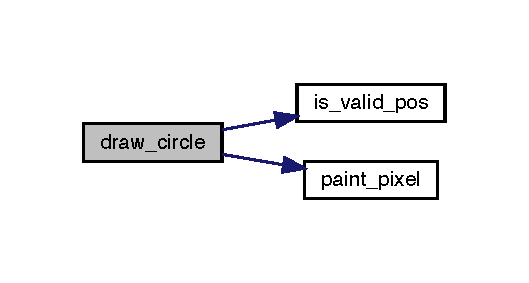
\includegraphics[width=254pt]{group__video__gr_ga6494f21641e972c58acdaedcf9c80520_cgraph}
\end{center}
\end{figure}
\hypertarget{group__video__gr_ga0b618a385e591f8690388281fd79a351}{}\label{group__video__gr_ga0b618a385e591f8690388281fd79a351} 
\index{video\+\_\+gr@{video\+\_\+gr}!draw\+\_\+line@{draw\+\_\+line}}
\index{draw\+\_\+line@{draw\+\_\+line}!video\+\_\+gr@{video\+\_\+gr}}
\subsubsection{\texorpdfstring{draw\+\_\+line()}{draw\_line()}}
{\footnotesize\ttfamily int draw\+\_\+line (\begin{DoxyParamCaption}\item[{unsigned short}]{xi,  }\item[{unsigned short}]{yi,  }\item[{unsigned short}]{xf,  }\item[{unsigned short}]{yf,  }\item[{uint16\+\_\+t}]{color }\end{DoxyParamCaption})}



Draws a line on the screen, given a color, a initial position and a final position. 


\begin{DoxyParams}{Parameters}
{\em xi} & Initial position of the line in the horizontal axis \\
\hline
{\em yi} & Initial position of the line in the vertical axis \\
\hline
{\em xf} & Final position of the line in the horizontal axis \\
\hline
{\em yf} & Final position of the line in the vertical axis \\
\hline
{\em color} & Color to paint the line\\
\hline
\end{DoxyParams}
\begin{DoxyReturn}{Returns}
Return 0 upon success, non-\/zero otherwise 
\end{DoxyReturn}
Here is the call graph for this function\+:\nopagebreak
\begin{figure}[H]
\begin{center}
\leavevmode
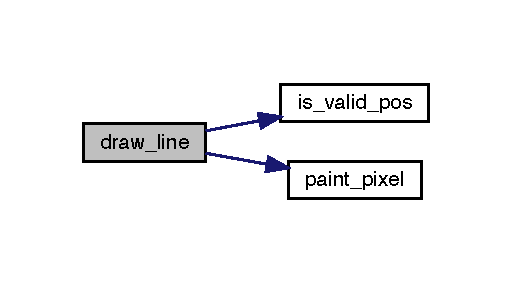
\includegraphics[width=246pt]{group__video__gr_ga0b618a385e591f8690388281fd79a351_cgraph}
\end{center}
\end{figure}
\hypertarget{group__video__gr_ga4270ae09ddc191cdc0e767e4412c386a}{}\label{group__video__gr_ga4270ae09ddc191cdc0e767e4412c386a} 
\index{video\+\_\+gr@{video\+\_\+gr}!draw\+\_\+missile@{draw\+\_\+missile}}
\index{draw\+\_\+missile@{draw\+\_\+missile}!video\+\_\+gr@{video\+\_\+gr}}
\subsubsection{\texorpdfstring{draw\+\_\+missile()}{draw\_missile()}}
{\footnotesize\ttfamily void draw\+\_\+missile (\begin{DoxyParamCaption}\item[{\hyperlink{group___missile_ga7ea98f7c879356e5dfa41934529d86e1}{Missile} $\ast$}]{ptr }\end{DoxyParamCaption})}



Draws a missile. 


\begin{DoxyParams}{Parameters}
{\em Pointer} & to the Missile in question \\
\hline
\end{DoxyParams}
Here is the call graph for this function\+:\nopagebreak
\begin{figure}[H]
\begin{center}
\leavevmode
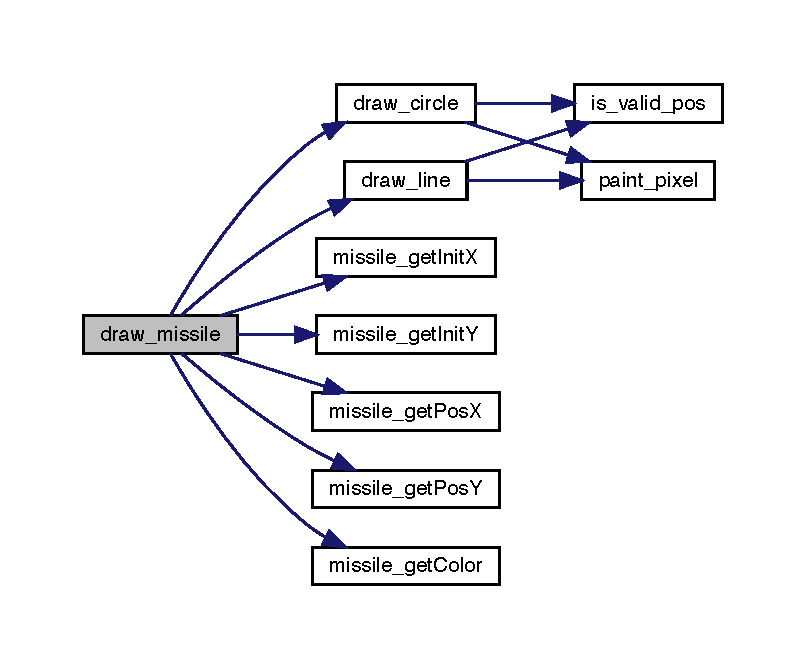
\includegraphics[width=350pt]{group__video__gr_ga4270ae09ddc191cdc0e767e4412c386a_cgraph}
\end{center}
\end{figure}
\hypertarget{group__video__gr_ga5cb0e000108ddc786148172ee56903c3}{}\label{group__video__gr_ga5cb0e000108ddc786148172ee56903c3} 
\index{video\+\_\+gr@{video\+\_\+gr}!draw\+\_\+mouse\+\_\+cross@{draw\+\_\+mouse\+\_\+cross}}
\index{draw\+\_\+mouse\+\_\+cross@{draw\+\_\+mouse\+\_\+cross}!video\+\_\+gr@{video\+\_\+gr}}
\subsubsection{\texorpdfstring{draw\+\_\+mouse\+\_\+cross()}{draw\_mouse\_cross()}}
{\footnotesize\ttfamily int draw\+\_\+mouse\+\_\+cross (\begin{DoxyParamCaption}\item[{const int $\ast$}]{mouse\+\_\+pos,  }\item[{uint16\+\_\+t}]{color }\end{DoxyParamCaption})}



Draws the mouse cross at a certain position with a certain color. 


\begin{DoxyParams}{Parameters}
{\em mouse\+\_\+pos} & Array containing the position of the mouse cross (x,y) \\
\hline
{\em color} & Color to paint the mouse cross\\
\hline
\end{DoxyParams}
\begin{DoxyReturn}{Returns}
Return 0 upon success, non-\/zero otherwise 
\end{DoxyReturn}
Here is the call graph for this function\+:\nopagebreak
\begin{figure}[H]
\begin{center}
\leavevmode
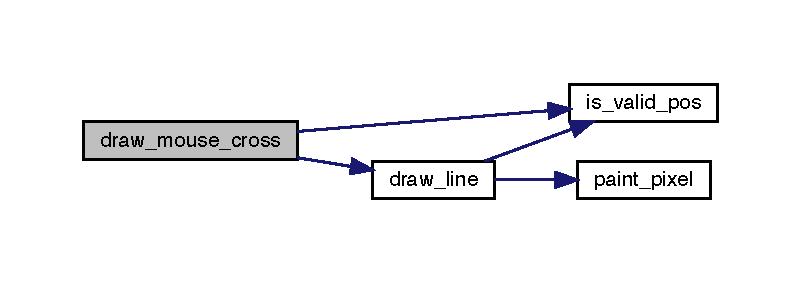
\includegraphics[width=350pt]{group__video__gr_ga5cb0e000108ddc786148172ee56903c3_cgraph}
\end{center}
\end{figure}
\hypertarget{group__video__gr_ga8dca584eb65462cd691cb94a9ec92602}{}\label{group__video__gr_ga8dca584eb65462cd691cb94a9ec92602} 
\index{video\+\_\+gr@{video\+\_\+gr}!draw\+\_\+number@{draw\+\_\+number}}
\index{draw\+\_\+number@{draw\+\_\+number}!video\+\_\+gr@{video\+\_\+gr}}
\subsubsection{\texorpdfstring{draw\+\_\+number()}{draw\_number()}}
{\footnotesize\ttfamily void draw\+\_\+number (\begin{DoxyParamCaption}\item[{unsigned}]{num,  }\item[{\hyperlink{struct_bitmap}{Bitmap} $\ast$$\ast$}]{font,  }\item[{unsigned}]{size\+\_\+x,  }\item[{unsigned}]{posX,  }\item[{unsigned}]{posY }\end{DoxyParamCaption})}



Draws a number at certain position. 


\begin{DoxyParams}{Parameters}
{\em num} & number to be drawn \\
\hline
{\em font} & Font used as an array of 10 numbers \\
\hline
{\em size\+\_\+x} & Horizontal size of the Font, in pixels \\
\hline
{\em posX} & Position of the number in the horizontal axis \\
\hline
{\em posY} & Position of the number in the vertical axis \\
\hline
\end{DoxyParams}
Here is the call graph for this function\+:\nopagebreak
\begin{figure}[H]
\begin{center}
\leavevmode
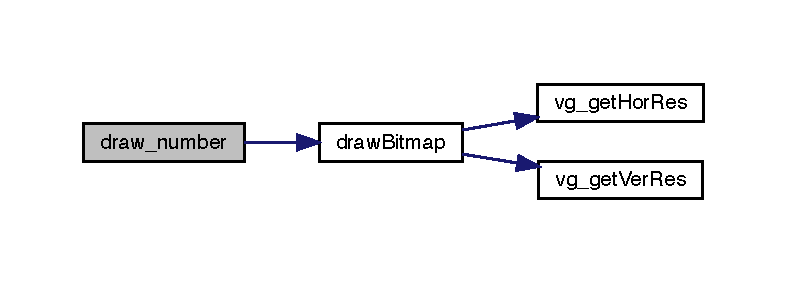
\includegraphics[width=350pt]{group__video__gr_ga8dca584eb65462cd691cb94a9ec92602_cgraph}
\end{center}
\end{figure}
\hypertarget{group__video__gr_ga07c3ec445f5548c09a75b0aacf262830}{}\label{group__video__gr_ga07c3ec445f5548c09a75b0aacf262830} 
\index{video\+\_\+gr@{video\+\_\+gr}!draw\+\_\+score@{draw\+\_\+score}}
\index{draw\+\_\+score@{draw\+\_\+score}!video\+\_\+gr@{video\+\_\+gr}}
\subsubsection{\texorpdfstring{draw\+\_\+score()}{draw\_score()}}
{\footnotesize\ttfamily void draw\+\_\+score (\begin{DoxyParamCaption}\item[{unsigned}]{num,  }\item[{unsigned}]{posX,  }\item[{unsigned}]{posY }\end{DoxyParamCaption})}



Draws a score at certain position. 


\begin{DoxyParams}{Parameters}
{\em num} & score to be drawn \\
\hline
{\em posX} & Position of the score in the horizontal axis \\
\hline
{\em posY} & Position of the score in the vertical axis \\
\hline
\end{DoxyParams}
Here is the call graph for this function\+:\nopagebreak
\begin{figure}[H]
\begin{center}
\leavevmode
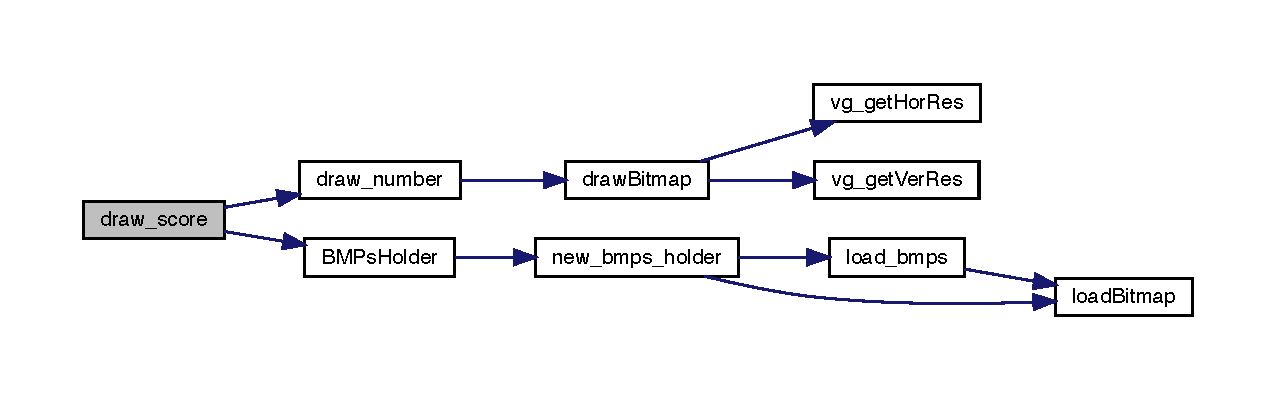
\includegraphics[width=350pt]{group__video__gr_ga07c3ec445f5548c09a75b0aacf262830_cgraph}
\end{center}
\end{figure}
\hypertarget{group__video__gr_ga975522708082967d9d107c340e6c01f5}{}\label{group__video__gr_ga975522708082967d9d107c340e6c01f5} 
\index{video\+\_\+gr@{video\+\_\+gr}!draw\+\_\+score\+\_\+big@{draw\+\_\+score\+\_\+big}}
\index{draw\+\_\+score\+\_\+big@{draw\+\_\+score\+\_\+big}!video\+\_\+gr@{video\+\_\+gr}}
\subsubsection{\texorpdfstring{draw\+\_\+score\+\_\+big()}{draw\_score\_big()}}
{\footnotesize\ttfamily void draw\+\_\+score\+\_\+big (\begin{DoxyParamCaption}\item[{unsigned}]{num,  }\item[{unsigned}]{posX,  }\item[{unsigned}]{posY }\end{DoxyParamCaption})}



Draws a big score at certain position. 

Similar to \hyperlink{group__video__gr_ga07c3ec445f5548c09a75b0aacf262830}{draw\+\_\+score()} but with larger numbers


\begin{DoxyParams}{Parameters}
{\em num} & score to be drawn \\
\hline
{\em posX} & Position of the big score in the horizontal axis \\
\hline
{\em posY} & Position of the big score in the vertical axis \\
\hline
\end{DoxyParams}
Here is the call graph for this function\+:\nopagebreak
\begin{figure}[H]
\begin{center}
\leavevmode
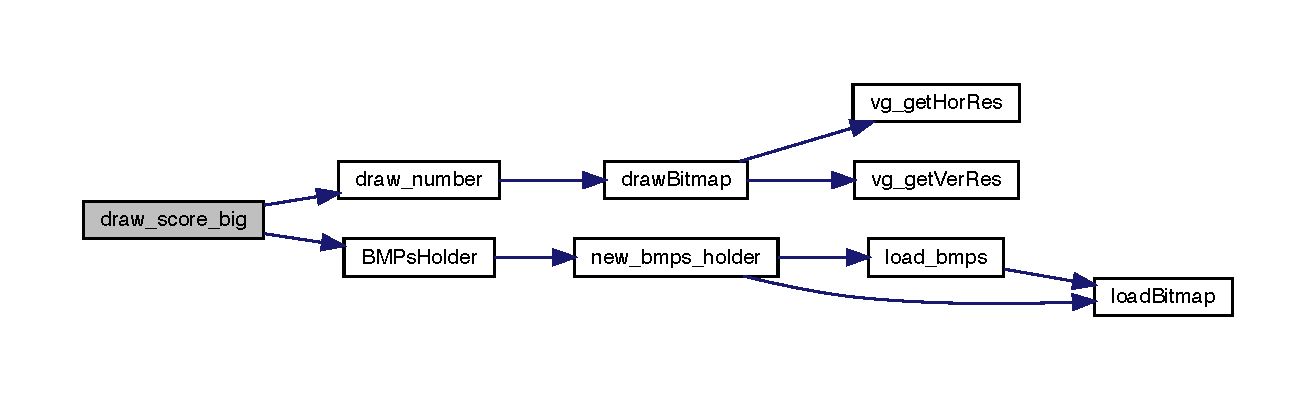
\includegraphics[width=350pt]{group__video__gr_ga975522708082967d9d107c340e6c01f5_cgraph}
\end{center}
\end{figure}
\hypertarget{group__video__gr_ga7f93731e89220a67419a16b1a415e133}{}\label{group__video__gr_ga7f93731e89220a67419a16b1a415e133} 
\index{video\+\_\+gr@{video\+\_\+gr}!is\+\_\+valid\+\_\+pos@{is\+\_\+valid\+\_\+pos}}
\index{is\+\_\+valid\+\_\+pos@{is\+\_\+valid\+\_\+pos}!video\+\_\+gr@{video\+\_\+gr}}
\subsubsection{\texorpdfstring{is\+\_\+valid\+\_\+pos()}{is\_valid\_pos()}}
{\footnotesize\ttfamily int is\+\_\+valid\+\_\+pos (\begin{DoxyParamCaption}\item[{unsigned short}]{x,  }\item[{unsigned short}]{y }\end{DoxyParamCaption})}



Checks if position (x,y) is inside the screen. 


\begin{DoxyParams}{Parameters}
{\em x} & Position in the horizontal axis \\
\hline
{\em y} & Position in the vertical axis\\
\hline
\end{DoxyParams}
\begin{DoxyReturn}{Returns}
Return 0 upon success, non-\/zero otherwise 
\end{DoxyReturn}
\hypertarget{group__video__gr_gafd0836c92e142e75c256799fb45032da}{}\label{group__video__gr_gafd0836c92e142e75c256799fb45032da} 
\index{video\+\_\+gr@{video\+\_\+gr}!paint\+\_\+pixel@{paint\+\_\+pixel}}
\index{paint\+\_\+pixel@{paint\+\_\+pixel}!video\+\_\+gr@{video\+\_\+gr}}
\subsubsection{\texorpdfstring{paint\+\_\+pixel()}{paint\_pixel()}}
{\footnotesize\ttfamily void paint\+\_\+pixel (\begin{DoxyParamCaption}\item[{int}]{x,  }\item[{int}]{y,  }\item[{uint16\+\_\+t}]{color }\end{DoxyParamCaption})}

the pixel at a certain position with a certain color


\begin{DoxyParams}{Parameters}
{\em x} & Position in the horizontal axis \\
\hline
{\em y} & Position in the vertical axis \\
\hline
{\em color} & Color to paint the pixel \\
\hline
\end{DoxyParams}
\hypertarget{group__video__gr_gafcc897567998ed3a26974926501a4abd}{}\label{group__video__gr_gafcc897567998ed3a26974926501a4abd} 
\index{video\+\_\+gr@{video\+\_\+gr}!rgb@{rgb}}
\index{rgb@{rgb}!video\+\_\+gr@{video\+\_\+gr}}
\subsubsection{\texorpdfstring{rgb()}{rgb()}}
{\footnotesize\ttfamily uint16\+\_\+t rgb (\begin{DoxyParamCaption}\item[{unsigned char}]{red\+\_\+value,  }\item[{unsigned char}]{green\+\_\+value,  }\item[{unsigned char}]{blue\+\_\+value }\end{DoxyParamCaption})}



Converts a rgb color to a hexadecimal of 6 bytes. 


\begin{DoxyParams}{Parameters}
{\em red\+\_\+value} & Value of red, between \mbox{[}0,255\mbox{]} \\
\hline
{\em red\+\_\+value} & Value of green, between \mbox{[}0,255\mbox{]} \\
\hline
{\em red\+\_\+value} & Value of blue, between \mbox{[}0,255\mbox{]} \\
\hline
\end{DoxyParams}
\hypertarget{group__video__gr_ga42f593e6656f1a978315aff02b1bcebf}{}\label{group__video__gr_ga42f593e6656f1a978315aff02b1bcebf} 
\index{video\+\_\+gr@{video\+\_\+gr}!vg\+\_\+exit@{vg\+\_\+exit}}
\index{vg\+\_\+exit@{vg\+\_\+exit}!video\+\_\+gr@{video\+\_\+gr}}
\subsubsection{\texorpdfstring{vg\+\_\+exit()}{vg\_exit()}}
{\footnotesize\ttfamily int vg\+\_\+exit (\begin{DoxyParamCaption}\item[{void}]{ }\end{DoxyParamCaption})}



Returns to default Minix 3 text mode (0x03\+: 25 x 80, 16 colors) 

\begin{DoxyReturn}{Returns}
Return 0 upon success, non-\/zero otherwise 
\end{DoxyReturn}
\hypertarget{group__video__gr_gabd51eef0a4ffcafb6a08fb40703f4383}{}\label{group__video__gr_gabd51eef0a4ffcafb6a08fb40703f4383} 
\index{video\+\_\+gr@{video\+\_\+gr}!vg\+\_\+get\+Buffer\+Ptr@{vg\+\_\+get\+Buffer\+Ptr}}
\index{vg\+\_\+get\+Buffer\+Ptr@{vg\+\_\+get\+Buffer\+Ptr}!video\+\_\+gr@{video\+\_\+gr}}
\subsubsection{\texorpdfstring{vg\+\_\+get\+Buffer\+Ptr()}{vg\_getBufferPtr()}}
{\footnotesize\ttfamily void$\ast$ vg\+\_\+get\+Buffer\+Ptr (\begin{DoxyParamCaption}{ }\end{DoxyParamCaption})}



Gets the pointer to the graphics Buffer used for double-\/buffering. 

\begin{DoxyReturn}{Returns}
Pointer to the graphics Buffer used for double-\/buffering 
\end{DoxyReturn}
\hypertarget{group__video__gr_gab3938dd22c03335341584d5b8f6752f5}{}\label{group__video__gr_gab3938dd22c03335341584d5b8f6752f5} 
\index{video\+\_\+gr@{video\+\_\+gr}!vg\+\_\+get\+Hor\+Res@{vg\+\_\+get\+Hor\+Res}}
\index{vg\+\_\+get\+Hor\+Res@{vg\+\_\+get\+Hor\+Res}!video\+\_\+gr@{video\+\_\+gr}}
\subsubsection{\texorpdfstring{vg\+\_\+get\+Hor\+Res()}{vg\_getHorRes()}}
{\footnotesize\ttfamily unsigned vg\+\_\+get\+Hor\+Res (\begin{DoxyParamCaption}{ }\end{DoxyParamCaption})}



Gets the horizontal Resolution of the screen. 

\begin{DoxyReturn}{Returns}
Return the horizontal Resolution of the screen 
\end{DoxyReturn}
\hypertarget{group__video__gr_gaab8200f7947926322b6dd6fa7c6da1e1}{}\label{group__video__gr_gaab8200f7947926322b6dd6fa7c6da1e1} 
\index{video\+\_\+gr@{video\+\_\+gr}!vg\+\_\+get\+Ver\+Res@{vg\+\_\+get\+Ver\+Res}}
\index{vg\+\_\+get\+Ver\+Res@{vg\+\_\+get\+Ver\+Res}!video\+\_\+gr@{video\+\_\+gr}}
\subsubsection{\texorpdfstring{vg\+\_\+get\+Ver\+Res()}{vg\_getVerRes()}}
{\footnotesize\ttfamily unsigned vg\+\_\+get\+Ver\+Res (\begin{DoxyParamCaption}{ }\end{DoxyParamCaption})}



Gets the vertical Resolution of the screen. 

\begin{DoxyReturn}{Returns}
Return the vertical Resolution of the screen 
\end{DoxyReturn}
\hypertarget{group__video__gr_ga7d19c24f10ca7bfb2c7b8f9e12d4dc6f}{}\label{group__video__gr_ga7d19c24f10ca7bfb2c7b8f9e12d4dc6f} 
\index{video\+\_\+gr@{video\+\_\+gr}!vg\+\_\+init@{vg\+\_\+init}}
\index{vg\+\_\+init@{vg\+\_\+init}!video\+\_\+gr@{video\+\_\+gr}}
\subsubsection{\texorpdfstring{vg\+\_\+init()}{vg\_init()}}
{\footnotesize\ttfamily int vg\+\_\+init (\begin{DoxyParamCaption}\item[{unsigned short}]{mode }\end{DoxyParamCaption})}



Initializes the video module in graphics mode. 

Uses the V\+BE I\+NT 0x10 interface to set the desired graphics mode, maps V\+R\+AM to the process\textquotesingle{} address space and initializes static global variables with the resolution of the screen, and the number of colors


\begin{DoxyParams}{Parameters}
{\em mode} & 16-\/bit V\+BE mode to set\\
\hline
\end{DoxyParams}
\begin{DoxyReturn}{Returns}
0 upon success, non-\/zero on failure 
\end{DoxyReturn}
Here is the call graph for this function\+:\nopagebreak
\begin{figure}[H]
\begin{center}
\leavevmode
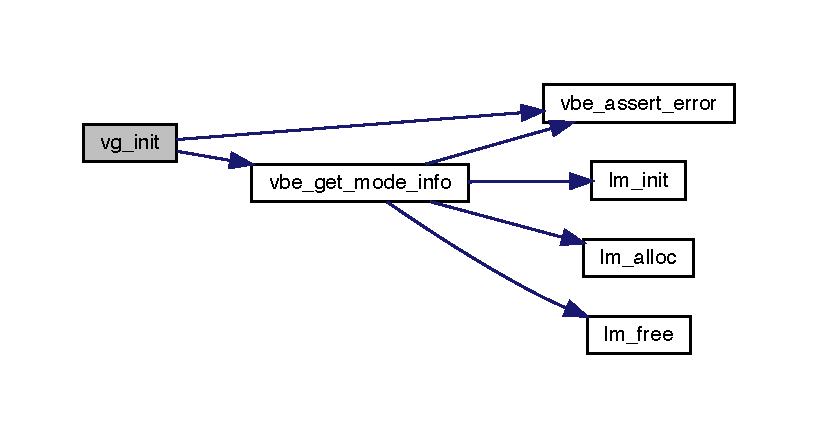
\includegraphics[width=350pt]{group__video__gr_ga7d19c24f10ca7bfb2c7b8f9e12d4dc6f_cgraph}
\end{center}
\end{figure}

\chapter{Class Documentation}
\hypertarget{struct____attribute____}{}\section{\+\_\+\+\_\+attribute\+\_\+\+\_\+ Struct Reference}
\label{struct____attribute____}\index{\+\_\+\+\_\+attribute\+\_\+\+\_\+@{\+\_\+\+\_\+attribute\+\_\+\+\_\+}}


{\ttfamily \#include $<$vbe.\+h$>$}

\subsection*{Public Attributes}
\begin{DoxyCompactItemize}
\item 
uint16\+\_\+t \hyperlink{struct____attribute_____a68ea99ad36679e583fa9674016e30903}{Mode\+Attributes}
\begin{DoxyCompactList}\small\item\em mode attributes \end{DoxyCompactList}\item 
uint8\+\_\+t \hyperlink{struct____attribute_____aeffe4dec59c5a757f65a97a66c812d3b}{Win\+A\+Attributes}
\begin{DoxyCompactList}\small\item\em window A attributes \end{DoxyCompactList}\item 
uint8\+\_\+t \hyperlink{struct____attribute_____ac9e21a3d7d22b24ed82be39f790b1408}{Win\+B\+Attributes}
\begin{DoxyCompactList}\small\item\em window B attributes \end{DoxyCompactList}\item 
uint16\+\_\+t \hyperlink{struct____attribute_____acc2114dbf039909e55cc3966abd3358d}{Win\+Granularity}
\begin{DoxyCompactList}\small\item\em window granularity \end{DoxyCompactList}\item 
uint16\+\_\+t \hyperlink{struct____attribute_____ad26e754fe362f3085c7ec4c0e5e75a6f}{Win\+Size}
\begin{DoxyCompactList}\small\item\em window size \end{DoxyCompactList}\item 
uint16\+\_\+t \hyperlink{struct____attribute_____a7cde26f911e3df97b7498ee139d8de12}{Win\+A\+Segment}
\begin{DoxyCompactList}\small\item\em window A start segment \end{DoxyCompactList}\item 
uint16\+\_\+t \hyperlink{struct____attribute_____a6dbaac9ee1cae36ca0c7b46559264b69}{Win\+B\+Segment}
\begin{DoxyCompactList}\small\item\em window B start segment \end{DoxyCompactList}\item 
phys\+\_\+bytes \hyperlink{struct____attribute_____aa211c2411f48f899b0bb0739ecef0b37}{Win\+Func\+Ptr}
\begin{DoxyCompactList}\small\item\em real mode/far pointer to window function \end{DoxyCompactList}\item 
uint16\+\_\+t \hyperlink{struct____attribute_____a3c9eb4b107ecee102c6e63f9054ede06}{Bytes\+Per\+Scan\+Line}
\begin{DoxyCompactList}\small\item\em bytes per scan line \end{DoxyCompactList}\item 
uint16\+\_\+t \hyperlink{struct____attribute_____abe48e2b29aa99e813a1447d22711f4f4}{X\+Resolution}
\begin{DoxyCompactList}\small\item\em horizontal resolution in pixels/characters \end{DoxyCompactList}\item 
uint16\+\_\+t \hyperlink{struct____attribute_____aa91385451d974d9c33978062e22d39e2}{Y\+Resolution}
\begin{DoxyCompactList}\small\item\em vertical resolution in pixels/characters \end{DoxyCompactList}\item 
uint8\+\_\+t \hyperlink{struct____attribute_____acac41a300563737d7849a92cd1d5c10b}{X\+Char\+Size}
\begin{DoxyCompactList}\small\item\em character cell width in pixels \end{DoxyCompactList}\item 
uint8\+\_\+t \hyperlink{struct____attribute_____acb93d86860efea5c87e3c2950f39123e}{Y\+Char\+Size}
\begin{DoxyCompactList}\small\item\em character cell height in pixels \end{DoxyCompactList}\item 
uint8\+\_\+t \hyperlink{struct____attribute_____ab1471d2f75e61117d65290da9070cf89}{Number\+Of\+Planes}
\begin{DoxyCompactList}\small\item\em number of memory planes \end{DoxyCompactList}\item 
uint8\+\_\+t \hyperlink{struct____attribute_____abd9c59af53589a54188bb57ada5c5f26}{Bits\+Per\+Pixel}
\begin{DoxyCompactList}\small\item\em bits per pixel \end{DoxyCompactList}\item 
uint8\+\_\+t \hyperlink{struct____attribute_____a59483378dd87414afcde6cb3ca93c2d8}{Number\+Of\+Banks}
\begin{DoxyCompactList}\small\item\em number of banks \end{DoxyCompactList}\item 
uint8\+\_\+t \hyperlink{struct____attribute_____a0fe34321b6dfba9e784fbbc649aa193a}{Memory\+Model}
\begin{DoxyCompactList}\small\item\em memory model type \end{DoxyCompactList}\item 
uint8\+\_\+t \hyperlink{struct____attribute_____aa1307567cbc12f9c5c724b7457be14ad}{Bank\+Size}
\begin{DoxyCompactList}\small\item\em bank size in KB \end{DoxyCompactList}\item 
uint8\+\_\+t \hyperlink{struct____attribute_____a988714bc16626547fbdc31f25dfa6470}{Number\+Of\+Image\+Pages}
\begin{DoxyCompactList}\small\item\em number of images \end{DoxyCompactList}\item 
uint8\+\_\+t \hyperlink{struct____attribute_____a8ace2dfe4814abc401442986ac8a5356}{Reserved1}
\begin{DoxyCompactList}\small\item\em reserved for page function \end{DoxyCompactList}\item 
uint8\+\_\+t \hyperlink{struct____attribute_____a9ffc14e11d6b1c80b63aba344292849e}{Red\+Mask\+Size}
\item 
uint8\+\_\+t \hyperlink{struct____attribute_____a8b5b2e458757061bce7e056f7f910dae}{Red\+Field\+Position}
\item 
uint8\+\_\+t \hyperlink{struct____attribute_____af69ef188a0f5d526ecd5f25a8d6336e3}{Green\+Mask\+Size}
\item 
uint8\+\_\+t \hyperlink{struct____attribute_____a44aab7c8026a131654e079837a95ba2b}{Green\+Field\+Position}
\item 
uint8\+\_\+t \hyperlink{struct____attribute_____ab5967602a79dcb7f0061195ffdaaa47a}{Blue\+Mask\+Size}
\item 
uint8\+\_\+t \hyperlink{struct____attribute_____ada852d5ed926757d24b5038a38e6292c}{Blue\+Field\+Position}
\item 
uint8\+\_\+t \hyperlink{struct____attribute_____a73862db83bdb9b6d31356af3cec7a5be}{Rsvd\+Mask\+Size}
\item 
uint8\+\_\+t \hyperlink{struct____attribute_____a61fb6dc07b7edbd8a3a94745336f256c}{Rsvd\+Field\+Position}
\item 
uint8\+\_\+t \hyperlink{struct____attribute_____a35fb3e1fc0dc9924bc52977b3a234f9f}{Direct\+Color\+Mode\+Info}
\item 
phys\+\_\+bytes \hyperlink{struct____attribute_____a852a4f68cfbabf08df197128e137bde6}{Phys\+Base\+Ptr}
\begin{DoxyCompactList}\small\item\em physical address for flat memory frame buffer \end{DoxyCompactList}\item 
uint8\+\_\+t \hyperlink{struct____attribute_____a534ebf7a2bdad17747cfc9cb6cc50c5c}{Reserved2} \mbox{[}4\mbox{]}
\begin{DoxyCompactList}\small\item\em Reserved -\/ always set to 0. \end{DoxyCompactList}\item 
uint8\+\_\+t \hyperlink{struct____attribute_____a9336499af9094522dbe1bfd4d43934a1}{Reserved3} \mbox{[}2\mbox{]}
\begin{DoxyCompactList}\small\item\em Reserved -\/ always set to 0. \end{DoxyCompactList}\item 
uint16\+\_\+t \hyperlink{struct____attribute_____af7036270c257deabc1ebd111faf3e3a5}{Lin\+Bytes\+Per\+Scan\+Line}
\item 
uint8\+\_\+t \hyperlink{struct____attribute_____ad5820084f2b821b85a635df8394f0d9e}{Bnk\+Number\+Of\+Image\+Pages}
\item 
uint8\+\_\+t \hyperlink{struct____attribute_____af9ba0d9902f5336bd9d044a9dee2ba42}{Lin\+Number\+Of\+Image\+Pages}
\item 
uint8\+\_\+t \hyperlink{struct____attribute_____a88a5ced225c9ef7ed6ffe33e5a39edc6}{Lin\+Red\+Mask\+Size}
\item 
uint8\+\_\+t \hyperlink{struct____attribute_____aec8d45f188ac9210b88216af83de847d}{Lin\+Red\+Field\+Position}
\item 
uint8\+\_\+t \hyperlink{struct____attribute_____a5768a84391f8a26d8a9bfd6a22d5e49d}{Lin\+Green\+Mask\+Size}
\item 
uint8\+\_\+t \hyperlink{struct____attribute_____a5571b1959950d520f2b45bb5549994e3}{Lin\+Green\+Field\+Position}
\item 
uint8\+\_\+t \hyperlink{struct____attribute_____aa2b79b8eed8d842e0db481fb1fbb9a06}{Lin\+Blue\+Mask\+Size}
\item 
uint8\+\_\+t \hyperlink{struct____attribute_____a99e6b6bdbda9f98f2823429dfd5b5685}{Lin\+Blue\+Field\+Position}
\item 
uint8\+\_\+t \hyperlink{struct____attribute_____a577b5892a22d06e230f528a62a472d1d}{Lin\+Rsvd\+Mask\+Size}
\item 
uint8\+\_\+t \hyperlink{struct____attribute_____a012126db503ad1281ae53aa41f4c96a7}{Lin\+Rsvd\+Field\+Position}
\item 
uint32\+\_\+t \hyperlink{struct____attribute_____afd81a69353c35e8b1fb9b696931f79a5}{Max\+Pixel\+Clock}
\item 
uint8\+\_\+t \hyperlink{struct____attribute_____ab859fb715f83f005dfa2f13d8b0e4ff0}{Reserved4} \mbox{[}190\mbox{]}
\item 
char \hyperlink{struct____attribute_____ae836dd2f0cf91de8d1387bc606feb595}{V\+E\+S\+A\+Signature} \mbox{[}4\mbox{]}
\item 
short \hyperlink{struct____attribute_____a14e4fe3377969955c48963300b715b37}{V\+E\+S\+A\+Version}
\item 
phys\+\_\+bytes \hyperlink{struct____attribute_____a6412609805e1bc6e48f7743a48dc841a}{O\+E\+M\+String\+Ptr}
\item 
long \hyperlink{struct____attribute_____a6dc2748c4ab226b9cbf6e7139fa24f74}{Capabilities}
\item 
phys\+\_\+bytes \hyperlink{struct____attribute_____ac3b2d0805352b33b6bb2610883e89e22}{Video\+Mode\+Ptr}
\item 
short \hyperlink{struct____attribute_____aad8c231af30c4ba0005f5bca523ecfc8}{Total\+Memory}
\item 
short \hyperlink{struct____attribute_____a4a00a2a7929046f2256d374d7182b3ad}{Oem\+Software\+Rev}
\item 
char $\ast$ \hyperlink{struct____attribute_____af0c799aee5a7aa7a1514217508e3f3ed}{Oem\+Vendor\+Name\+Ptr}
\item 
char $\ast$ \hyperlink{struct____attribute_____acbda83ed0529a356cecb49583996960f}{Oem\+Product\+Name\+Ptr}
\item 
char $\ast$ \hyperlink{struct____attribute_____ab4343da5f260d2438dc5c64feb9636bf}{Oem\+Product\+Rev\+Ptr}
\item 
char \hyperlink{struct____attribute_____a009ec7baf4ee08c85717a2d5c63a277b}{reserved} \mbox{[}222\mbox{]}
\item 
char \hyperlink{struct____attribute_____a1001bc87085a4c9669331941dfd3be59}{Oem\+Data} \mbox{[}256\mbox{]}
\end{DoxyCompactItemize}


\subsection{Detailed Description}
Packed V\+BE Mode Info Block 

\subsection{Member Data Documentation}
\hypertarget{struct____attribute_____aa1307567cbc12f9c5c724b7457be14ad}{}\label{struct____attribute_____aa1307567cbc12f9c5c724b7457be14ad} 
\index{\+\_\+\+\_\+attribute\+\_\+\+\_\+@{\+\_\+\+\_\+attribute\+\_\+\+\_\+}!Bank\+Size@{Bank\+Size}}
\index{Bank\+Size@{Bank\+Size}!\+\_\+\+\_\+attribute\+\_\+\+\_\+@{\+\_\+\+\_\+attribute\+\_\+\+\_\+}}
\subsubsection{\texorpdfstring{Bank\+Size}{BankSize}}
{\footnotesize\ttfamily uint8\+\_\+t \+\_\+\+\_\+attribute\+\_\+\+\_\+\+::\+Bank\+Size}



bank size in KB 

\hypertarget{struct____attribute_____abd9c59af53589a54188bb57ada5c5f26}{}\label{struct____attribute_____abd9c59af53589a54188bb57ada5c5f26} 
\index{\+\_\+\+\_\+attribute\+\_\+\+\_\+@{\+\_\+\+\_\+attribute\+\_\+\+\_\+}!Bits\+Per\+Pixel@{Bits\+Per\+Pixel}}
\index{Bits\+Per\+Pixel@{Bits\+Per\+Pixel}!\+\_\+\+\_\+attribute\+\_\+\+\_\+@{\+\_\+\+\_\+attribute\+\_\+\+\_\+}}
\subsubsection{\texorpdfstring{Bits\+Per\+Pixel}{BitsPerPixel}}
{\footnotesize\ttfamily uint8\+\_\+t \+\_\+\+\_\+attribute\+\_\+\+\_\+\+::\+Bits\+Per\+Pixel}



bits per pixel 

\hypertarget{struct____attribute_____ada852d5ed926757d24b5038a38e6292c}{}\label{struct____attribute_____ada852d5ed926757d24b5038a38e6292c} 
\index{\+\_\+\+\_\+attribute\+\_\+\+\_\+@{\+\_\+\+\_\+attribute\+\_\+\+\_\+}!Blue\+Field\+Position@{Blue\+Field\+Position}}
\index{Blue\+Field\+Position@{Blue\+Field\+Position}!\+\_\+\+\_\+attribute\+\_\+\+\_\+@{\+\_\+\+\_\+attribute\+\_\+\+\_\+}}
\subsubsection{\texorpdfstring{Blue\+Field\+Position}{BlueFieldPosition}}
{\footnotesize\ttfamily uint8\+\_\+t \+\_\+\+\_\+attribute\+\_\+\+\_\+\+::\+Blue\+Field\+Position}

\hypertarget{struct____attribute_____ab5967602a79dcb7f0061195ffdaaa47a}{}\label{struct____attribute_____ab5967602a79dcb7f0061195ffdaaa47a} 
\index{\+\_\+\+\_\+attribute\+\_\+\+\_\+@{\+\_\+\+\_\+attribute\+\_\+\+\_\+}!Blue\+Mask\+Size@{Blue\+Mask\+Size}}
\index{Blue\+Mask\+Size@{Blue\+Mask\+Size}!\+\_\+\+\_\+attribute\+\_\+\+\_\+@{\+\_\+\+\_\+attribute\+\_\+\+\_\+}}
\subsubsection{\texorpdfstring{Blue\+Mask\+Size}{BlueMaskSize}}
{\footnotesize\ttfamily uint8\+\_\+t \+\_\+\+\_\+attribute\+\_\+\+\_\+\+::\+Blue\+Mask\+Size}

\hypertarget{struct____attribute_____ad5820084f2b821b85a635df8394f0d9e}{}\label{struct____attribute_____ad5820084f2b821b85a635df8394f0d9e} 
\index{\+\_\+\+\_\+attribute\+\_\+\+\_\+@{\+\_\+\+\_\+attribute\+\_\+\+\_\+}!Bnk\+Number\+Of\+Image\+Pages@{Bnk\+Number\+Of\+Image\+Pages}}
\index{Bnk\+Number\+Of\+Image\+Pages@{Bnk\+Number\+Of\+Image\+Pages}!\+\_\+\+\_\+attribute\+\_\+\+\_\+@{\+\_\+\+\_\+attribute\+\_\+\+\_\+}}
\subsubsection{\texorpdfstring{Bnk\+Number\+Of\+Image\+Pages}{BnkNumberOfImagePages}}
{\footnotesize\ttfamily uint8\+\_\+t \+\_\+\+\_\+attribute\+\_\+\+\_\+\+::\+Bnk\+Number\+Of\+Image\+Pages}

\hypertarget{struct____attribute_____a3c9eb4b107ecee102c6e63f9054ede06}{}\label{struct____attribute_____a3c9eb4b107ecee102c6e63f9054ede06} 
\index{\+\_\+\+\_\+attribute\+\_\+\+\_\+@{\+\_\+\+\_\+attribute\+\_\+\+\_\+}!Bytes\+Per\+Scan\+Line@{Bytes\+Per\+Scan\+Line}}
\index{Bytes\+Per\+Scan\+Line@{Bytes\+Per\+Scan\+Line}!\+\_\+\+\_\+attribute\+\_\+\+\_\+@{\+\_\+\+\_\+attribute\+\_\+\+\_\+}}
\subsubsection{\texorpdfstring{Bytes\+Per\+Scan\+Line}{BytesPerScanLine}}
{\footnotesize\ttfamily uint16\+\_\+t \+\_\+\+\_\+attribute\+\_\+\+\_\+\+::\+Bytes\+Per\+Scan\+Line}



bytes per scan line 

\hypertarget{struct____attribute_____a6dc2748c4ab226b9cbf6e7139fa24f74}{}\label{struct____attribute_____a6dc2748c4ab226b9cbf6e7139fa24f74} 
\index{\+\_\+\+\_\+attribute\+\_\+\+\_\+@{\+\_\+\+\_\+attribute\+\_\+\+\_\+}!Capabilities@{Capabilities}}
\index{Capabilities@{Capabilities}!\+\_\+\+\_\+attribute\+\_\+\+\_\+@{\+\_\+\+\_\+attribute\+\_\+\+\_\+}}
\subsubsection{\texorpdfstring{Capabilities}{Capabilities}}
{\footnotesize\ttfamily long \+\_\+\+\_\+attribute\+\_\+\+\_\+\+::\+Capabilities}

\hypertarget{struct____attribute_____a35fb3e1fc0dc9924bc52977b3a234f9f}{}\label{struct____attribute_____a35fb3e1fc0dc9924bc52977b3a234f9f} 
\index{\+\_\+\+\_\+attribute\+\_\+\+\_\+@{\+\_\+\+\_\+attribute\+\_\+\+\_\+}!Direct\+Color\+Mode\+Info@{Direct\+Color\+Mode\+Info}}
\index{Direct\+Color\+Mode\+Info@{Direct\+Color\+Mode\+Info}!\+\_\+\+\_\+attribute\+\_\+\+\_\+@{\+\_\+\+\_\+attribute\+\_\+\+\_\+}}
\subsubsection{\texorpdfstring{Direct\+Color\+Mode\+Info}{DirectColorModeInfo}}
{\footnotesize\ttfamily uint8\+\_\+t \+\_\+\+\_\+attribute\+\_\+\+\_\+\+::\+Direct\+Color\+Mode\+Info}

\hypertarget{struct____attribute_____a44aab7c8026a131654e079837a95ba2b}{}\label{struct____attribute_____a44aab7c8026a131654e079837a95ba2b} 
\index{\+\_\+\+\_\+attribute\+\_\+\+\_\+@{\+\_\+\+\_\+attribute\+\_\+\+\_\+}!Green\+Field\+Position@{Green\+Field\+Position}}
\index{Green\+Field\+Position@{Green\+Field\+Position}!\+\_\+\+\_\+attribute\+\_\+\+\_\+@{\+\_\+\+\_\+attribute\+\_\+\+\_\+}}
\subsubsection{\texorpdfstring{Green\+Field\+Position}{GreenFieldPosition}}
{\footnotesize\ttfamily uint8\+\_\+t \+\_\+\+\_\+attribute\+\_\+\+\_\+\+::\+Green\+Field\+Position}

\hypertarget{struct____attribute_____af69ef188a0f5d526ecd5f25a8d6336e3}{}\label{struct____attribute_____af69ef188a0f5d526ecd5f25a8d6336e3} 
\index{\+\_\+\+\_\+attribute\+\_\+\+\_\+@{\+\_\+\+\_\+attribute\+\_\+\+\_\+}!Green\+Mask\+Size@{Green\+Mask\+Size}}
\index{Green\+Mask\+Size@{Green\+Mask\+Size}!\+\_\+\+\_\+attribute\+\_\+\+\_\+@{\+\_\+\+\_\+attribute\+\_\+\+\_\+}}
\subsubsection{\texorpdfstring{Green\+Mask\+Size}{GreenMaskSize}}
{\footnotesize\ttfamily uint8\+\_\+t \+\_\+\+\_\+attribute\+\_\+\+\_\+\+::\+Green\+Mask\+Size}

\hypertarget{struct____attribute_____a99e6b6bdbda9f98f2823429dfd5b5685}{}\label{struct____attribute_____a99e6b6bdbda9f98f2823429dfd5b5685} 
\index{\+\_\+\+\_\+attribute\+\_\+\+\_\+@{\+\_\+\+\_\+attribute\+\_\+\+\_\+}!Lin\+Blue\+Field\+Position@{Lin\+Blue\+Field\+Position}}
\index{Lin\+Blue\+Field\+Position@{Lin\+Blue\+Field\+Position}!\+\_\+\+\_\+attribute\+\_\+\+\_\+@{\+\_\+\+\_\+attribute\+\_\+\+\_\+}}
\subsubsection{\texorpdfstring{Lin\+Blue\+Field\+Position}{LinBlueFieldPosition}}
{\footnotesize\ttfamily uint8\+\_\+t \+\_\+\+\_\+attribute\+\_\+\+\_\+\+::\+Lin\+Blue\+Field\+Position}

\hypertarget{struct____attribute_____aa2b79b8eed8d842e0db481fb1fbb9a06}{}\label{struct____attribute_____aa2b79b8eed8d842e0db481fb1fbb9a06} 
\index{\+\_\+\+\_\+attribute\+\_\+\+\_\+@{\+\_\+\+\_\+attribute\+\_\+\+\_\+}!Lin\+Blue\+Mask\+Size@{Lin\+Blue\+Mask\+Size}}
\index{Lin\+Blue\+Mask\+Size@{Lin\+Blue\+Mask\+Size}!\+\_\+\+\_\+attribute\+\_\+\+\_\+@{\+\_\+\+\_\+attribute\+\_\+\+\_\+}}
\subsubsection{\texorpdfstring{Lin\+Blue\+Mask\+Size}{LinBlueMaskSize}}
{\footnotesize\ttfamily uint8\+\_\+t \+\_\+\+\_\+attribute\+\_\+\+\_\+\+::\+Lin\+Blue\+Mask\+Size}

\hypertarget{struct____attribute_____af7036270c257deabc1ebd111faf3e3a5}{}\label{struct____attribute_____af7036270c257deabc1ebd111faf3e3a5} 
\index{\+\_\+\+\_\+attribute\+\_\+\+\_\+@{\+\_\+\+\_\+attribute\+\_\+\+\_\+}!Lin\+Bytes\+Per\+Scan\+Line@{Lin\+Bytes\+Per\+Scan\+Line}}
\index{Lin\+Bytes\+Per\+Scan\+Line@{Lin\+Bytes\+Per\+Scan\+Line}!\+\_\+\+\_\+attribute\+\_\+\+\_\+@{\+\_\+\+\_\+attribute\+\_\+\+\_\+}}
\subsubsection{\texorpdfstring{Lin\+Bytes\+Per\+Scan\+Line}{LinBytesPerScanLine}}
{\footnotesize\ttfamily uint16\+\_\+t \+\_\+\+\_\+attribute\+\_\+\+\_\+\+::\+Lin\+Bytes\+Per\+Scan\+Line}

\hypertarget{struct____attribute_____a5571b1959950d520f2b45bb5549994e3}{}\label{struct____attribute_____a5571b1959950d520f2b45bb5549994e3} 
\index{\+\_\+\+\_\+attribute\+\_\+\+\_\+@{\+\_\+\+\_\+attribute\+\_\+\+\_\+}!Lin\+Green\+Field\+Position@{Lin\+Green\+Field\+Position}}
\index{Lin\+Green\+Field\+Position@{Lin\+Green\+Field\+Position}!\+\_\+\+\_\+attribute\+\_\+\+\_\+@{\+\_\+\+\_\+attribute\+\_\+\+\_\+}}
\subsubsection{\texorpdfstring{Lin\+Green\+Field\+Position}{LinGreenFieldPosition}}
{\footnotesize\ttfamily uint8\+\_\+t \+\_\+\+\_\+attribute\+\_\+\+\_\+\+::\+Lin\+Green\+Field\+Position}

\hypertarget{struct____attribute_____a5768a84391f8a26d8a9bfd6a22d5e49d}{}\label{struct____attribute_____a5768a84391f8a26d8a9bfd6a22d5e49d} 
\index{\+\_\+\+\_\+attribute\+\_\+\+\_\+@{\+\_\+\+\_\+attribute\+\_\+\+\_\+}!Lin\+Green\+Mask\+Size@{Lin\+Green\+Mask\+Size}}
\index{Lin\+Green\+Mask\+Size@{Lin\+Green\+Mask\+Size}!\+\_\+\+\_\+attribute\+\_\+\+\_\+@{\+\_\+\+\_\+attribute\+\_\+\+\_\+}}
\subsubsection{\texorpdfstring{Lin\+Green\+Mask\+Size}{LinGreenMaskSize}}
{\footnotesize\ttfamily uint8\+\_\+t \+\_\+\+\_\+attribute\+\_\+\+\_\+\+::\+Lin\+Green\+Mask\+Size}

\hypertarget{struct____attribute_____af9ba0d9902f5336bd9d044a9dee2ba42}{}\label{struct____attribute_____af9ba0d9902f5336bd9d044a9dee2ba42} 
\index{\+\_\+\+\_\+attribute\+\_\+\+\_\+@{\+\_\+\+\_\+attribute\+\_\+\+\_\+}!Lin\+Number\+Of\+Image\+Pages@{Lin\+Number\+Of\+Image\+Pages}}
\index{Lin\+Number\+Of\+Image\+Pages@{Lin\+Number\+Of\+Image\+Pages}!\+\_\+\+\_\+attribute\+\_\+\+\_\+@{\+\_\+\+\_\+attribute\+\_\+\+\_\+}}
\subsubsection{\texorpdfstring{Lin\+Number\+Of\+Image\+Pages}{LinNumberOfImagePages}}
{\footnotesize\ttfamily uint8\+\_\+t \+\_\+\+\_\+attribute\+\_\+\+\_\+\+::\+Lin\+Number\+Of\+Image\+Pages}

\hypertarget{struct____attribute_____aec8d45f188ac9210b88216af83de847d}{}\label{struct____attribute_____aec8d45f188ac9210b88216af83de847d} 
\index{\+\_\+\+\_\+attribute\+\_\+\+\_\+@{\+\_\+\+\_\+attribute\+\_\+\+\_\+}!Lin\+Red\+Field\+Position@{Lin\+Red\+Field\+Position}}
\index{Lin\+Red\+Field\+Position@{Lin\+Red\+Field\+Position}!\+\_\+\+\_\+attribute\+\_\+\+\_\+@{\+\_\+\+\_\+attribute\+\_\+\+\_\+}}
\subsubsection{\texorpdfstring{Lin\+Red\+Field\+Position}{LinRedFieldPosition}}
{\footnotesize\ttfamily uint8\+\_\+t \+\_\+\+\_\+attribute\+\_\+\+\_\+\+::\+Lin\+Red\+Field\+Position}

\hypertarget{struct____attribute_____a88a5ced225c9ef7ed6ffe33e5a39edc6}{}\label{struct____attribute_____a88a5ced225c9ef7ed6ffe33e5a39edc6} 
\index{\+\_\+\+\_\+attribute\+\_\+\+\_\+@{\+\_\+\+\_\+attribute\+\_\+\+\_\+}!Lin\+Red\+Mask\+Size@{Lin\+Red\+Mask\+Size}}
\index{Lin\+Red\+Mask\+Size@{Lin\+Red\+Mask\+Size}!\+\_\+\+\_\+attribute\+\_\+\+\_\+@{\+\_\+\+\_\+attribute\+\_\+\+\_\+}}
\subsubsection{\texorpdfstring{Lin\+Red\+Mask\+Size}{LinRedMaskSize}}
{\footnotesize\ttfamily uint8\+\_\+t \+\_\+\+\_\+attribute\+\_\+\+\_\+\+::\+Lin\+Red\+Mask\+Size}

\hypertarget{struct____attribute_____a012126db503ad1281ae53aa41f4c96a7}{}\label{struct____attribute_____a012126db503ad1281ae53aa41f4c96a7} 
\index{\+\_\+\+\_\+attribute\+\_\+\+\_\+@{\+\_\+\+\_\+attribute\+\_\+\+\_\+}!Lin\+Rsvd\+Field\+Position@{Lin\+Rsvd\+Field\+Position}}
\index{Lin\+Rsvd\+Field\+Position@{Lin\+Rsvd\+Field\+Position}!\+\_\+\+\_\+attribute\+\_\+\+\_\+@{\+\_\+\+\_\+attribute\+\_\+\+\_\+}}
\subsubsection{\texorpdfstring{Lin\+Rsvd\+Field\+Position}{LinRsvdFieldPosition}}
{\footnotesize\ttfamily uint8\+\_\+t \+\_\+\+\_\+attribute\+\_\+\+\_\+\+::\+Lin\+Rsvd\+Field\+Position}

\hypertarget{struct____attribute_____a577b5892a22d06e230f528a62a472d1d}{}\label{struct____attribute_____a577b5892a22d06e230f528a62a472d1d} 
\index{\+\_\+\+\_\+attribute\+\_\+\+\_\+@{\+\_\+\+\_\+attribute\+\_\+\+\_\+}!Lin\+Rsvd\+Mask\+Size@{Lin\+Rsvd\+Mask\+Size}}
\index{Lin\+Rsvd\+Mask\+Size@{Lin\+Rsvd\+Mask\+Size}!\+\_\+\+\_\+attribute\+\_\+\+\_\+@{\+\_\+\+\_\+attribute\+\_\+\+\_\+}}
\subsubsection{\texorpdfstring{Lin\+Rsvd\+Mask\+Size}{LinRsvdMaskSize}}
{\footnotesize\ttfamily uint8\+\_\+t \+\_\+\+\_\+attribute\+\_\+\+\_\+\+::\+Lin\+Rsvd\+Mask\+Size}

\hypertarget{struct____attribute_____afd81a69353c35e8b1fb9b696931f79a5}{}\label{struct____attribute_____afd81a69353c35e8b1fb9b696931f79a5} 
\index{\+\_\+\+\_\+attribute\+\_\+\+\_\+@{\+\_\+\+\_\+attribute\+\_\+\+\_\+}!Max\+Pixel\+Clock@{Max\+Pixel\+Clock}}
\index{Max\+Pixel\+Clock@{Max\+Pixel\+Clock}!\+\_\+\+\_\+attribute\+\_\+\+\_\+@{\+\_\+\+\_\+attribute\+\_\+\+\_\+}}
\subsubsection{\texorpdfstring{Max\+Pixel\+Clock}{MaxPixelClock}}
{\footnotesize\ttfamily uint32\+\_\+t \+\_\+\+\_\+attribute\+\_\+\+\_\+\+::\+Max\+Pixel\+Clock}

\hypertarget{struct____attribute_____a0fe34321b6dfba9e784fbbc649aa193a}{}\label{struct____attribute_____a0fe34321b6dfba9e784fbbc649aa193a} 
\index{\+\_\+\+\_\+attribute\+\_\+\+\_\+@{\+\_\+\+\_\+attribute\+\_\+\+\_\+}!Memory\+Model@{Memory\+Model}}
\index{Memory\+Model@{Memory\+Model}!\+\_\+\+\_\+attribute\+\_\+\+\_\+@{\+\_\+\+\_\+attribute\+\_\+\+\_\+}}
\subsubsection{\texorpdfstring{Memory\+Model}{MemoryModel}}
{\footnotesize\ttfamily uint8\+\_\+t \+\_\+\+\_\+attribute\+\_\+\+\_\+\+::\+Memory\+Model}



memory model type 

\hypertarget{struct____attribute_____a68ea99ad36679e583fa9674016e30903}{}\label{struct____attribute_____a68ea99ad36679e583fa9674016e30903} 
\index{\+\_\+\+\_\+attribute\+\_\+\+\_\+@{\+\_\+\+\_\+attribute\+\_\+\+\_\+}!Mode\+Attributes@{Mode\+Attributes}}
\index{Mode\+Attributes@{Mode\+Attributes}!\+\_\+\+\_\+attribute\+\_\+\+\_\+@{\+\_\+\+\_\+attribute\+\_\+\+\_\+}}
\subsubsection{\texorpdfstring{Mode\+Attributes}{ModeAttributes}}
{\footnotesize\ttfamily uint16\+\_\+t \+\_\+\+\_\+attribute\+\_\+\+\_\+\+::\+Mode\+Attributes}



mode attributes 

\hypertarget{struct____attribute_____a59483378dd87414afcde6cb3ca93c2d8}{}\label{struct____attribute_____a59483378dd87414afcde6cb3ca93c2d8} 
\index{\+\_\+\+\_\+attribute\+\_\+\+\_\+@{\+\_\+\+\_\+attribute\+\_\+\+\_\+}!Number\+Of\+Banks@{Number\+Of\+Banks}}
\index{Number\+Of\+Banks@{Number\+Of\+Banks}!\+\_\+\+\_\+attribute\+\_\+\+\_\+@{\+\_\+\+\_\+attribute\+\_\+\+\_\+}}
\subsubsection{\texorpdfstring{Number\+Of\+Banks}{NumberOfBanks}}
{\footnotesize\ttfamily uint8\+\_\+t \+\_\+\+\_\+attribute\+\_\+\+\_\+\+::\+Number\+Of\+Banks}



number of banks 

\hypertarget{struct____attribute_____a988714bc16626547fbdc31f25dfa6470}{}\label{struct____attribute_____a988714bc16626547fbdc31f25dfa6470} 
\index{\+\_\+\+\_\+attribute\+\_\+\+\_\+@{\+\_\+\+\_\+attribute\+\_\+\+\_\+}!Number\+Of\+Image\+Pages@{Number\+Of\+Image\+Pages}}
\index{Number\+Of\+Image\+Pages@{Number\+Of\+Image\+Pages}!\+\_\+\+\_\+attribute\+\_\+\+\_\+@{\+\_\+\+\_\+attribute\+\_\+\+\_\+}}
\subsubsection{\texorpdfstring{Number\+Of\+Image\+Pages}{NumberOfImagePages}}
{\footnotesize\ttfamily uint8\+\_\+t \+\_\+\+\_\+attribute\+\_\+\+\_\+\+::\+Number\+Of\+Image\+Pages}



number of images 

\hypertarget{struct____attribute_____ab1471d2f75e61117d65290da9070cf89}{}\label{struct____attribute_____ab1471d2f75e61117d65290da9070cf89} 
\index{\+\_\+\+\_\+attribute\+\_\+\+\_\+@{\+\_\+\+\_\+attribute\+\_\+\+\_\+}!Number\+Of\+Planes@{Number\+Of\+Planes}}
\index{Number\+Of\+Planes@{Number\+Of\+Planes}!\+\_\+\+\_\+attribute\+\_\+\+\_\+@{\+\_\+\+\_\+attribute\+\_\+\+\_\+}}
\subsubsection{\texorpdfstring{Number\+Of\+Planes}{NumberOfPlanes}}
{\footnotesize\ttfamily uint8\+\_\+t \+\_\+\+\_\+attribute\+\_\+\+\_\+\+::\+Number\+Of\+Planes}



number of memory planes 

\hypertarget{struct____attribute_____a1001bc87085a4c9669331941dfd3be59}{}\label{struct____attribute_____a1001bc87085a4c9669331941dfd3be59} 
\index{\+\_\+\+\_\+attribute\+\_\+\+\_\+@{\+\_\+\+\_\+attribute\+\_\+\+\_\+}!Oem\+Data@{Oem\+Data}}
\index{Oem\+Data@{Oem\+Data}!\+\_\+\+\_\+attribute\+\_\+\+\_\+@{\+\_\+\+\_\+attribute\+\_\+\+\_\+}}
\subsubsection{\texorpdfstring{Oem\+Data}{OemData}}
{\footnotesize\ttfamily char \+\_\+\+\_\+attribute\+\_\+\+\_\+\+::\+Oem\+Data\mbox{[}256\mbox{]}}

\hypertarget{struct____attribute_____acbda83ed0529a356cecb49583996960f}{}\label{struct____attribute_____acbda83ed0529a356cecb49583996960f} 
\index{\+\_\+\+\_\+attribute\+\_\+\+\_\+@{\+\_\+\+\_\+attribute\+\_\+\+\_\+}!Oem\+Product\+Name\+Ptr@{Oem\+Product\+Name\+Ptr}}
\index{Oem\+Product\+Name\+Ptr@{Oem\+Product\+Name\+Ptr}!\+\_\+\+\_\+attribute\+\_\+\+\_\+@{\+\_\+\+\_\+attribute\+\_\+\+\_\+}}
\subsubsection{\texorpdfstring{Oem\+Product\+Name\+Ptr}{OemProductNamePtr}}
{\footnotesize\ttfamily char$\ast$ \+\_\+\+\_\+attribute\+\_\+\+\_\+\+::\+Oem\+Product\+Name\+Ptr}

\hypertarget{struct____attribute_____ab4343da5f260d2438dc5c64feb9636bf}{}\label{struct____attribute_____ab4343da5f260d2438dc5c64feb9636bf} 
\index{\+\_\+\+\_\+attribute\+\_\+\+\_\+@{\+\_\+\+\_\+attribute\+\_\+\+\_\+}!Oem\+Product\+Rev\+Ptr@{Oem\+Product\+Rev\+Ptr}}
\index{Oem\+Product\+Rev\+Ptr@{Oem\+Product\+Rev\+Ptr}!\+\_\+\+\_\+attribute\+\_\+\+\_\+@{\+\_\+\+\_\+attribute\+\_\+\+\_\+}}
\subsubsection{\texorpdfstring{Oem\+Product\+Rev\+Ptr}{OemProductRevPtr}}
{\footnotesize\ttfamily char$\ast$ \+\_\+\+\_\+attribute\+\_\+\+\_\+\+::\+Oem\+Product\+Rev\+Ptr}

\hypertarget{struct____attribute_____a4a00a2a7929046f2256d374d7182b3ad}{}\label{struct____attribute_____a4a00a2a7929046f2256d374d7182b3ad} 
\index{\+\_\+\+\_\+attribute\+\_\+\+\_\+@{\+\_\+\+\_\+attribute\+\_\+\+\_\+}!Oem\+Software\+Rev@{Oem\+Software\+Rev}}
\index{Oem\+Software\+Rev@{Oem\+Software\+Rev}!\+\_\+\+\_\+attribute\+\_\+\+\_\+@{\+\_\+\+\_\+attribute\+\_\+\+\_\+}}
\subsubsection{\texorpdfstring{Oem\+Software\+Rev}{OemSoftwareRev}}
{\footnotesize\ttfamily short \+\_\+\+\_\+attribute\+\_\+\+\_\+\+::\+Oem\+Software\+Rev}

\hypertarget{struct____attribute_____a6412609805e1bc6e48f7743a48dc841a}{}\label{struct____attribute_____a6412609805e1bc6e48f7743a48dc841a} 
\index{\+\_\+\+\_\+attribute\+\_\+\+\_\+@{\+\_\+\+\_\+attribute\+\_\+\+\_\+}!O\+E\+M\+String\+Ptr@{O\+E\+M\+String\+Ptr}}
\index{O\+E\+M\+String\+Ptr@{O\+E\+M\+String\+Ptr}!\+\_\+\+\_\+attribute\+\_\+\+\_\+@{\+\_\+\+\_\+attribute\+\_\+\+\_\+}}
\subsubsection{\texorpdfstring{O\+E\+M\+String\+Ptr}{OEMStringPtr}}
{\footnotesize\ttfamily phys\+\_\+bytes \+\_\+\+\_\+attribute\+\_\+\+\_\+\+::\+O\+E\+M\+String\+Ptr}

\hypertarget{struct____attribute_____af0c799aee5a7aa7a1514217508e3f3ed}{}\label{struct____attribute_____af0c799aee5a7aa7a1514217508e3f3ed} 
\index{\+\_\+\+\_\+attribute\+\_\+\+\_\+@{\+\_\+\+\_\+attribute\+\_\+\+\_\+}!Oem\+Vendor\+Name\+Ptr@{Oem\+Vendor\+Name\+Ptr}}
\index{Oem\+Vendor\+Name\+Ptr@{Oem\+Vendor\+Name\+Ptr}!\+\_\+\+\_\+attribute\+\_\+\+\_\+@{\+\_\+\+\_\+attribute\+\_\+\+\_\+}}
\subsubsection{\texorpdfstring{Oem\+Vendor\+Name\+Ptr}{OemVendorNamePtr}}
{\footnotesize\ttfamily char$\ast$ \+\_\+\+\_\+attribute\+\_\+\+\_\+\+::\+Oem\+Vendor\+Name\+Ptr}

\hypertarget{struct____attribute_____a852a4f68cfbabf08df197128e137bde6}{}\label{struct____attribute_____a852a4f68cfbabf08df197128e137bde6} 
\index{\+\_\+\+\_\+attribute\+\_\+\+\_\+@{\+\_\+\+\_\+attribute\+\_\+\+\_\+}!Phys\+Base\+Ptr@{Phys\+Base\+Ptr}}
\index{Phys\+Base\+Ptr@{Phys\+Base\+Ptr}!\+\_\+\+\_\+attribute\+\_\+\+\_\+@{\+\_\+\+\_\+attribute\+\_\+\+\_\+}}
\subsubsection{\texorpdfstring{Phys\+Base\+Ptr}{PhysBasePtr}}
{\footnotesize\ttfamily phys\+\_\+bytes \+\_\+\+\_\+attribute\+\_\+\+\_\+\+::\+Phys\+Base\+Ptr}



physical address for flat memory frame buffer 

\hypertarget{struct____attribute_____a8b5b2e458757061bce7e056f7f910dae}{}\label{struct____attribute_____a8b5b2e458757061bce7e056f7f910dae} 
\index{\+\_\+\+\_\+attribute\+\_\+\+\_\+@{\+\_\+\+\_\+attribute\+\_\+\+\_\+}!Red\+Field\+Position@{Red\+Field\+Position}}
\index{Red\+Field\+Position@{Red\+Field\+Position}!\+\_\+\+\_\+attribute\+\_\+\+\_\+@{\+\_\+\+\_\+attribute\+\_\+\+\_\+}}
\subsubsection{\texorpdfstring{Red\+Field\+Position}{RedFieldPosition}}
{\footnotesize\ttfamily uint8\+\_\+t \+\_\+\+\_\+attribute\+\_\+\+\_\+\+::\+Red\+Field\+Position}

\hypertarget{struct____attribute_____a9ffc14e11d6b1c80b63aba344292849e}{}\label{struct____attribute_____a9ffc14e11d6b1c80b63aba344292849e} 
\index{\+\_\+\+\_\+attribute\+\_\+\+\_\+@{\+\_\+\+\_\+attribute\+\_\+\+\_\+}!Red\+Mask\+Size@{Red\+Mask\+Size}}
\index{Red\+Mask\+Size@{Red\+Mask\+Size}!\+\_\+\+\_\+attribute\+\_\+\+\_\+@{\+\_\+\+\_\+attribute\+\_\+\+\_\+}}
\subsubsection{\texorpdfstring{Red\+Mask\+Size}{RedMaskSize}}
{\footnotesize\ttfamily uint8\+\_\+t \+\_\+\+\_\+attribute\+\_\+\+\_\+\+::\+Red\+Mask\+Size}

\hypertarget{struct____attribute_____a009ec7baf4ee08c85717a2d5c63a277b}{}\label{struct____attribute_____a009ec7baf4ee08c85717a2d5c63a277b} 
\index{\+\_\+\+\_\+attribute\+\_\+\+\_\+@{\+\_\+\+\_\+attribute\+\_\+\+\_\+}!reserved@{reserved}}
\index{reserved@{reserved}!\+\_\+\+\_\+attribute\+\_\+\+\_\+@{\+\_\+\+\_\+attribute\+\_\+\+\_\+}}
\subsubsection{\texorpdfstring{reserved}{reserved}}
{\footnotesize\ttfamily char \+\_\+\+\_\+attribute\+\_\+\+\_\+\+::reserved\mbox{[}222\mbox{]}}

\hypertarget{struct____attribute_____a8ace2dfe4814abc401442986ac8a5356}{}\label{struct____attribute_____a8ace2dfe4814abc401442986ac8a5356} 
\index{\+\_\+\+\_\+attribute\+\_\+\+\_\+@{\+\_\+\+\_\+attribute\+\_\+\+\_\+}!Reserved1@{Reserved1}}
\index{Reserved1@{Reserved1}!\+\_\+\+\_\+attribute\+\_\+\+\_\+@{\+\_\+\+\_\+attribute\+\_\+\+\_\+}}
\subsubsection{\texorpdfstring{Reserved1}{Reserved1}}
{\footnotesize\ttfamily uint8\+\_\+t \+\_\+\+\_\+attribute\+\_\+\+\_\+\+::\+Reserved1}



reserved for page function 

\hypertarget{struct____attribute_____a534ebf7a2bdad17747cfc9cb6cc50c5c}{}\label{struct____attribute_____a534ebf7a2bdad17747cfc9cb6cc50c5c} 
\index{\+\_\+\+\_\+attribute\+\_\+\+\_\+@{\+\_\+\+\_\+attribute\+\_\+\+\_\+}!Reserved2@{Reserved2}}
\index{Reserved2@{Reserved2}!\+\_\+\+\_\+attribute\+\_\+\+\_\+@{\+\_\+\+\_\+attribute\+\_\+\+\_\+}}
\subsubsection{\texorpdfstring{Reserved2}{Reserved2}}
{\footnotesize\ttfamily uint8\+\_\+t \+\_\+\+\_\+attribute\+\_\+\+\_\+\+::\+Reserved2\mbox{[}4\mbox{]}}



Reserved -\/ always set to 0. 

\hypertarget{struct____attribute_____a9336499af9094522dbe1bfd4d43934a1}{}\label{struct____attribute_____a9336499af9094522dbe1bfd4d43934a1} 
\index{\+\_\+\+\_\+attribute\+\_\+\+\_\+@{\+\_\+\+\_\+attribute\+\_\+\+\_\+}!Reserved3@{Reserved3}}
\index{Reserved3@{Reserved3}!\+\_\+\+\_\+attribute\+\_\+\+\_\+@{\+\_\+\+\_\+attribute\+\_\+\+\_\+}}
\subsubsection{\texorpdfstring{Reserved3}{Reserved3}}
{\footnotesize\ttfamily uint8\+\_\+t \+\_\+\+\_\+attribute\+\_\+\+\_\+\+::\+Reserved3\mbox{[}2\mbox{]}}



Reserved -\/ always set to 0. 

\hypertarget{struct____attribute_____ab859fb715f83f005dfa2f13d8b0e4ff0}{}\label{struct____attribute_____ab859fb715f83f005dfa2f13d8b0e4ff0} 
\index{\+\_\+\+\_\+attribute\+\_\+\+\_\+@{\+\_\+\+\_\+attribute\+\_\+\+\_\+}!Reserved4@{Reserved4}}
\index{Reserved4@{Reserved4}!\+\_\+\+\_\+attribute\+\_\+\+\_\+@{\+\_\+\+\_\+attribute\+\_\+\+\_\+}}
\subsubsection{\texorpdfstring{Reserved4}{Reserved4}}
{\footnotesize\ttfamily uint8\+\_\+t \+\_\+\+\_\+attribute\+\_\+\+\_\+\+::\+Reserved4\mbox{[}190\mbox{]}}

\hypertarget{struct____attribute_____a61fb6dc07b7edbd8a3a94745336f256c}{}\label{struct____attribute_____a61fb6dc07b7edbd8a3a94745336f256c} 
\index{\+\_\+\+\_\+attribute\+\_\+\+\_\+@{\+\_\+\+\_\+attribute\+\_\+\+\_\+}!Rsvd\+Field\+Position@{Rsvd\+Field\+Position}}
\index{Rsvd\+Field\+Position@{Rsvd\+Field\+Position}!\+\_\+\+\_\+attribute\+\_\+\+\_\+@{\+\_\+\+\_\+attribute\+\_\+\+\_\+}}
\subsubsection{\texorpdfstring{Rsvd\+Field\+Position}{RsvdFieldPosition}}
{\footnotesize\ttfamily uint8\+\_\+t \+\_\+\+\_\+attribute\+\_\+\+\_\+\+::\+Rsvd\+Field\+Position}

\hypertarget{struct____attribute_____a73862db83bdb9b6d31356af3cec7a5be}{}\label{struct____attribute_____a73862db83bdb9b6d31356af3cec7a5be} 
\index{\+\_\+\+\_\+attribute\+\_\+\+\_\+@{\+\_\+\+\_\+attribute\+\_\+\+\_\+}!Rsvd\+Mask\+Size@{Rsvd\+Mask\+Size}}
\index{Rsvd\+Mask\+Size@{Rsvd\+Mask\+Size}!\+\_\+\+\_\+attribute\+\_\+\+\_\+@{\+\_\+\+\_\+attribute\+\_\+\+\_\+}}
\subsubsection{\texorpdfstring{Rsvd\+Mask\+Size}{RsvdMaskSize}}
{\footnotesize\ttfamily uint8\+\_\+t \+\_\+\+\_\+attribute\+\_\+\+\_\+\+::\+Rsvd\+Mask\+Size}

\hypertarget{struct____attribute_____aad8c231af30c4ba0005f5bca523ecfc8}{}\label{struct____attribute_____aad8c231af30c4ba0005f5bca523ecfc8} 
\index{\+\_\+\+\_\+attribute\+\_\+\+\_\+@{\+\_\+\+\_\+attribute\+\_\+\+\_\+}!Total\+Memory@{Total\+Memory}}
\index{Total\+Memory@{Total\+Memory}!\+\_\+\+\_\+attribute\+\_\+\+\_\+@{\+\_\+\+\_\+attribute\+\_\+\+\_\+}}
\subsubsection{\texorpdfstring{Total\+Memory}{TotalMemory}}
{\footnotesize\ttfamily short \+\_\+\+\_\+attribute\+\_\+\+\_\+\+::\+Total\+Memory}

\hypertarget{struct____attribute_____ae836dd2f0cf91de8d1387bc606feb595}{}\label{struct____attribute_____ae836dd2f0cf91de8d1387bc606feb595} 
\index{\+\_\+\+\_\+attribute\+\_\+\+\_\+@{\+\_\+\+\_\+attribute\+\_\+\+\_\+}!V\+E\+S\+A\+Signature@{V\+E\+S\+A\+Signature}}
\index{V\+E\+S\+A\+Signature@{V\+E\+S\+A\+Signature}!\+\_\+\+\_\+attribute\+\_\+\+\_\+@{\+\_\+\+\_\+attribute\+\_\+\+\_\+}}
\subsubsection{\texorpdfstring{V\+E\+S\+A\+Signature}{VESASignature}}
{\footnotesize\ttfamily char \+\_\+\+\_\+attribute\+\_\+\+\_\+\+::\+V\+E\+S\+A\+Signature\mbox{[}4\mbox{]}}

\hypertarget{struct____attribute_____a14e4fe3377969955c48963300b715b37}{}\label{struct____attribute_____a14e4fe3377969955c48963300b715b37} 
\index{\+\_\+\+\_\+attribute\+\_\+\+\_\+@{\+\_\+\+\_\+attribute\+\_\+\+\_\+}!V\+E\+S\+A\+Version@{V\+E\+S\+A\+Version}}
\index{V\+E\+S\+A\+Version@{V\+E\+S\+A\+Version}!\+\_\+\+\_\+attribute\+\_\+\+\_\+@{\+\_\+\+\_\+attribute\+\_\+\+\_\+}}
\subsubsection{\texorpdfstring{V\+E\+S\+A\+Version}{VESAVersion}}
{\footnotesize\ttfamily short \+\_\+\+\_\+attribute\+\_\+\+\_\+\+::\+V\+E\+S\+A\+Version}

\hypertarget{struct____attribute_____ac3b2d0805352b33b6bb2610883e89e22}{}\label{struct____attribute_____ac3b2d0805352b33b6bb2610883e89e22} 
\index{\+\_\+\+\_\+attribute\+\_\+\+\_\+@{\+\_\+\+\_\+attribute\+\_\+\+\_\+}!Video\+Mode\+Ptr@{Video\+Mode\+Ptr}}
\index{Video\+Mode\+Ptr@{Video\+Mode\+Ptr}!\+\_\+\+\_\+attribute\+\_\+\+\_\+@{\+\_\+\+\_\+attribute\+\_\+\+\_\+}}
\subsubsection{\texorpdfstring{Video\+Mode\+Ptr}{VideoModePtr}}
{\footnotesize\ttfamily phys\+\_\+bytes \+\_\+\+\_\+attribute\+\_\+\+\_\+\+::\+Video\+Mode\+Ptr}

\hypertarget{struct____attribute_____aeffe4dec59c5a757f65a97a66c812d3b}{}\label{struct____attribute_____aeffe4dec59c5a757f65a97a66c812d3b} 
\index{\+\_\+\+\_\+attribute\+\_\+\+\_\+@{\+\_\+\+\_\+attribute\+\_\+\+\_\+}!Win\+A\+Attributes@{Win\+A\+Attributes}}
\index{Win\+A\+Attributes@{Win\+A\+Attributes}!\+\_\+\+\_\+attribute\+\_\+\+\_\+@{\+\_\+\+\_\+attribute\+\_\+\+\_\+}}
\subsubsection{\texorpdfstring{Win\+A\+Attributes}{WinAAttributes}}
{\footnotesize\ttfamily uint8\+\_\+t \+\_\+\+\_\+attribute\+\_\+\+\_\+\+::\+Win\+A\+Attributes}



window A attributes 

\hypertarget{struct____attribute_____a7cde26f911e3df97b7498ee139d8de12}{}\label{struct____attribute_____a7cde26f911e3df97b7498ee139d8de12} 
\index{\+\_\+\+\_\+attribute\+\_\+\+\_\+@{\+\_\+\+\_\+attribute\+\_\+\+\_\+}!Win\+A\+Segment@{Win\+A\+Segment}}
\index{Win\+A\+Segment@{Win\+A\+Segment}!\+\_\+\+\_\+attribute\+\_\+\+\_\+@{\+\_\+\+\_\+attribute\+\_\+\+\_\+}}
\subsubsection{\texorpdfstring{Win\+A\+Segment}{WinASegment}}
{\footnotesize\ttfamily uint16\+\_\+t \+\_\+\+\_\+attribute\+\_\+\+\_\+\+::\+Win\+A\+Segment}



window A start segment 

\hypertarget{struct____attribute_____ac9e21a3d7d22b24ed82be39f790b1408}{}\label{struct____attribute_____ac9e21a3d7d22b24ed82be39f790b1408} 
\index{\+\_\+\+\_\+attribute\+\_\+\+\_\+@{\+\_\+\+\_\+attribute\+\_\+\+\_\+}!Win\+B\+Attributes@{Win\+B\+Attributes}}
\index{Win\+B\+Attributes@{Win\+B\+Attributes}!\+\_\+\+\_\+attribute\+\_\+\+\_\+@{\+\_\+\+\_\+attribute\+\_\+\+\_\+}}
\subsubsection{\texorpdfstring{Win\+B\+Attributes}{WinBAttributes}}
{\footnotesize\ttfamily uint8\+\_\+t \+\_\+\+\_\+attribute\+\_\+\+\_\+\+::\+Win\+B\+Attributes}



window B attributes 

\hypertarget{struct____attribute_____a6dbaac9ee1cae36ca0c7b46559264b69}{}\label{struct____attribute_____a6dbaac9ee1cae36ca0c7b46559264b69} 
\index{\+\_\+\+\_\+attribute\+\_\+\+\_\+@{\+\_\+\+\_\+attribute\+\_\+\+\_\+}!Win\+B\+Segment@{Win\+B\+Segment}}
\index{Win\+B\+Segment@{Win\+B\+Segment}!\+\_\+\+\_\+attribute\+\_\+\+\_\+@{\+\_\+\+\_\+attribute\+\_\+\+\_\+}}
\subsubsection{\texorpdfstring{Win\+B\+Segment}{WinBSegment}}
{\footnotesize\ttfamily uint16\+\_\+t \+\_\+\+\_\+attribute\+\_\+\+\_\+\+::\+Win\+B\+Segment}



window B start segment 

\hypertarget{struct____attribute_____aa211c2411f48f899b0bb0739ecef0b37}{}\label{struct____attribute_____aa211c2411f48f899b0bb0739ecef0b37} 
\index{\+\_\+\+\_\+attribute\+\_\+\+\_\+@{\+\_\+\+\_\+attribute\+\_\+\+\_\+}!Win\+Func\+Ptr@{Win\+Func\+Ptr}}
\index{Win\+Func\+Ptr@{Win\+Func\+Ptr}!\+\_\+\+\_\+attribute\+\_\+\+\_\+@{\+\_\+\+\_\+attribute\+\_\+\+\_\+}}
\subsubsection{\texorpdfstring{Win\+Func\+Ptr}{WinFuncPtr}}
{\footnotesize\ttfamily phys\+\_\+bytes \+\_\+\+\_\+attribute\+\_\+\+\_\+\+::\+Win\+Func\+Ptr}



real mode/far pointer to window function 

\hypertarget{struct____attribute_____acc2114dbf039909e55cc3966abd3358d}{}\label{struct____attribute_____acc2114dbf039909e55cc3966abd3358d} 
\index{\+\_\+\+\_\+attribute\+\_\+\+\_\+@{\+\_\+\+\_\+attribute\+\_\+\+\_\+}!Win\+Granularity@{Win\+Granularity}}
\index{Win\+Granularity@{Win\+Granularity}!\+\_\+\+\_\+attribute\+\_\+\+\_\+@{\+\_\+\+\_\+attribute\+\_\+\+\_\+}}
\subsubsection{\texorpdfstring{Win\+Granularity}{WinGranularity}}
{\footnotesize\ttfamily uint16\+\_\+t \+\_\+\+\_\+attribute\+\_\+\+\_\+\+::\+Win\+Granularity}



window granularity 

\hypertarget{struct____attribute_____ad26e754fe362f3085c7ec4c0e5e75a6f}{}\label{struct____attribute_____ad26e754fe362f3085c7ec4c0e5e75a6f} 
\index{\+\_\+\+\_\+attribute\+\_\+\+\_\+@{\+\_\+\+\_\+attribute\+\_\+\+\_\+}!Win\+Size@{Win\+Size}}
\index{Win\+Size@{Win\+Size}!\+\_\+\+\_\+attribute\+\_\+\+\_\+@{\+\_\+\+\_\+attribute\+\_\+\+\_\+}}
\subsubsection{\texorpdfstring{Win\+Size}{WinSize}}
{\footnotesize\ttfamily uint16\+\_\+t \+\_\+\+\_\+attribute\+\_\+\+\_\+\+::\+Win\+Size}



window size 

\hypertarget{struct____attribute_____acac41a300563737d7849a92cd1d5c10b}{}\label{struct____attribute_____acac41a300563737d7849a92cd1d5c10b} 
\index{\+\_\+\+\_\+attribute\+\_\+\+\_\+@{\+\_\+\+\_\+attribute\+\_\+\+\_\+}!X\+Char\+Size@{X\+Char\+Size}}
\index{X\+Char\+Size@{X\+Char\+Size}!\+\_\+\+\_\+attribute\+\_\+\+\_\+@{\+\_\+\+\_\+attribute\+\_\+\+\_\+}}
\subsubsection{\texorpdfstring{X\+Char\+Size}{XCharSize}}
{\footnotesize\ttfamily uint8\+\_\+t \+\_\+\+\_\+attribute\+\_\+\+\_\+\+::\+X\+Char\+Size}



character cell width in pixels 

\hypertarget{struct____attribute_____abe48e2b29aa99e813a1447d22711f4f4}{}\label{struct____attribute_____abe48e2b29aa99e813a1447d22711f4f4} 
\index{\+\_\+\+\_\+attribute\+\_\+\+\_\+@{\+\_\+\+\_\+attribute\+\_\+\+\_\+}!X\+Resolution@{X\+Resolution}}
\index{X\+Resolution@{X\+Resolution}!\+\_\+\+\_\+attribute\+\_\+\+\_\+@{\+\_\+\+\_\+attribute\+\_\+\+\_\+}}
\subsubsection{\texorpdfstring{X\+Resolution}{XResolution}}
{\footnotesize\ttfamily uint16\+\_\+t \+\_\+\+\_\+attribute\+\_\+\+\_\+\+::\+X\+Resolution}



horizontal resolution in pixels/characters 

\hypertarget{struct____attribute_____acb93d86860efea5c87e3c2950f39123e}{}\label{struct____attribute_____acb93d86860efea5c87e3c2950f39123e} 
\index{\+\_\+\+\_\+attribute\+\_\+\+\_\+@{\+\_\+\+\_\+attribute\+\_\+\+\_\+}!Y\+Char\+Size@{Y\+Char\+Size}}
\index{Y\+Char\+Size@{Y\+Char\+Size}!\+\_\+\+\_\+attribute\+\_\+\+\_\+@{\+\_\+\+\_\+attribute\+\_\+\+\_\+}}
\subsubsection{\texorpdfstring{Y\+Char\+Size}{YCharSize}}
{\footnotesize\ttfamily uint8\+\_\+t \+\_\+\+\_\+attribute\+\_\+\+\_\+\+::\+Y\+Char\+Size}



character cell height in pixels 

\hypertarget{struct____attribute_____aa91385451d974d9c33978062e22d39e2}{}\label{struct____attribute_____aa91385451d974d9c33978062e22d39e2} 
\index{\+\_\+\+\_\+attribute\+\_\+\+\_\+@{\+\_\+\+\_\+attribute\+\_\+\+\_\+}!Y\+Resolution@{Y\+Resolution}}
\index{Y\+Resolution@{Y\+Resolution}!\+\_\+\+\_\+attribute\+\_\+\+\_\+@{\+\_\+\+\_\+attribute\+\_\+\+\_\+}}
\subsubsection{\texorpdfstring{Y\+Resolution}{YResolution}}
{\footnotesize\ttfamily uint16\+\_\+t \+\_\+\+\_\+attribute\+\_\+\+\_\+\+::\+Y\+Resolution}



vertical resolution in pixels/characters 



The documentation for this struct was generated from the following file\+:\begin{DoxyCompactItemize}
\item 
/\+Users/andre/\+Documents/lcom1617-\/t4g01/proj/src/\hyperlink{vbe_8h}{vbe.\+h}\end{DoxyCompactItemize}

\hypertarget{struct_bitmap}{}\section{Bitmap Struct Reference}
\label{struct_bitmap}\index{Bitmap@{Bitmap}}


Represents a \hyperlink{struct_bitmap}{Bitmap}.  




{\ttfamily \#include $<$Bitmap.\+h$>$}



Collaboration diagram for Bitmap\+:\nopagebreak
\begin{figure}[H]
\begin{center}
\leavevmode
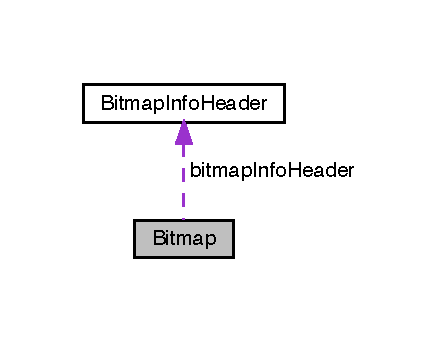
\includegraphics[width=211pt]{struct_bitmap__coll__graph}
\end{center}
\end{figure}
\subsection*{Public Attributes}
\begin{DoxyCompactItemize}
\item 
\hyperlink{struct_bitmap_info_header}{Bitmap\+Info\+Header} \hyperlink{struct_bitmap_a95c481a5ce1ff4af08cd135ca4af120b}{bitmap\+Info\+Header}
\item 
unsigned char $\ast$ \hyperlink{struct_bitmap_a581eac36ec50d730299b6df60e644750}{bitmap\+Data}
\end{DoxyCompactItemize}


\subsection{Detailed Description}
Represents a \hyperlink{struct_bitmap}{Bitmap}. 

\subsection{Member Data Documentation}
\hypertarget{struct_bitmap_a581eac36ec50d730299b6df60e644750}{}\label{struct_bitmap_a581eac36ec50d730299b6df60e644750} 
\index{Bitmap@{Bitmap}!bitmap\+Data@{bitmap\+Data}}
\index{bitmap\+Data@{bitmap\+Data}!Bitmap@{Bitmap}}
\subsubsection{\texorpdfstring{bitmap\+Data}{bitmapData}}
{\footnotesize\ttfamily unsigned char$\ast$ Bitmap\+::bitmap\+Data}

\hypertarget{struct_bitmap_a95c481a5ce1ff4af08cd135ca4af120b}{}\label{struct_bitmap_a95c481a5ce1ff4af08cd135ca4af120b} 
\index{Bitmap@{Bitmap}!bitmap\+Info\+Header@{bitmap\+Info\+Header}}
\index{bitmap\+Info\+Header@{bitmap\+Info\+Header}!Bitmap@{Bitmap}}
\subsubsection{\texorpdfstring{bitmap\+Info\+Header}{bitmapInfoHeader}}
{\footnotesize\ttfamily \hyperlink{struct_bitmap_info_header}{Bitmap\+Info\+Header} Bitmap\+::bitmap\+Info\+Header}



The documentation for this struct was generated from the following file\+:\begin{DoxyCompactItemize}
\item 
/\+Users/andre/\+Documents/lcom1617-\/t4g01/proj/src/\hyperlink{_bitmap_8h}{Bitmap.\+h}\end{DoxyCompactItemize}

\hypertarget{struct_bitmap_file_header}{}\section{Bitmap\+File\+Header Struct Reference}
\label{struct_bitmap_file_header}\index{Bitmap\+File\+Header@{Bitmap\+File\+Header}}


{\ttfamily \#include $<$Bitmap.\+h$>$}

\subsection*{Public Attributes}
\begin{DoxyCompactItemize}
\item 
unsigned short \hyperlink{struct_bitmap_file_header_a139c2c2645bc00ddf4f5dc552872c1d1}{type}
\item 
unsigned int \hyperlink{struct_bitmap_file_header_a0dcad71d9b17783c4d296c2c6d00ede0}{size}
\item 
unsigned int \hyperlink{struct_bitmap_file_header_ab3833d77e2c28a216859a80ba8fac9f0}{reserved}
\item 
unsigned int \hyperlink{struct_bitmap_file_header_a26ed598693b100ffd9e29c4dc77f3d92}{offset}
\end{DoxyCompactItemize}


\subsection{Member Data Documentation}
\hypertarget{struct_bitmap_file_header_a26ed598693b100ffd9e29c4dc77f3d92}{}\label{struct_bitmap_file_header_a26ed598693b100ffd9e29c4dc77f3d92} 
\index{Bitmap\+File\+Header@{Bitmap\+File\+Header}!offset@{offset}}
\index{offset@{offset}!Bitmap\+File\+Header@{Bitmap\+File\+Header}}
\subsubsection{\texorpdfstring{offset}{offset}}
{\footnotesize\ttfamily unsigned int Bitmap\+File\+Header\+::offset}

\hypertarget{struct_bitmap_file_header_ab3833d77e2c28a216859a80ba8fac9f0}{}\label{struct_bitmap_file_header_ab3833d77e2c28a216859a80ba8fac9f0} 
\index{Bitmap\+File\+Header@{Bitmap\+File\+Header}!reserved@{reserved}}
\index{reserved@{reserved}!Bitmap\+File\+Header@{Bitmap\+File\+Header}}
\subsubsection{\texorpdfstring{reserved}{reserved}}
{\footnotesize\ttfamily unsigned int Bitmap\+File\+Header\+::reserved}

\hypertarget{struct_bitmap_file_header_a0dcad71d9b17783c4d296c2c6d00ede0}{}\label{struct_bitmap_file_header_a0dcad71d9b17783c4d296c2c6d00ede0} 
\index{Bitmap\+File\+Header@{Bitmap\+File\+Header}!size@{size}}
\index{size@{size}!Bitmap\+File\+Header@{Bitmap\+File\+Header}}
\subsubsection{\texorpdfstring{size}{size}}
{\footnotesize\ttfamily unsigned int Bitmap\+File\+Header\+::size}

\hypertarget{struct_bitmap_file_header_a139c2c2645bc00ddf4f5dc552872c1d1}{}\label{struct_bitmap_file_header_a139c2c2645bc00ddf4f5dc552872c1d1} 
\index{Bitmap\+File\+Header@{Bitmap\+File\+Header}!type@{type}}
\index{type@{type}!Bitmap\+File\+Header@{Bitmap\+File\+Header}}
\subsubsection{\texorpdfstring{type}{type}}
{\footnotesize\ttfamily unsigned short Bitmap\+File\+Header\+::type}



The documentation for this struct was generated from the following file\+:\begin{DoxyCompactItemize}
\item 
/\+Users/andre/\+Documents/lcom1617-\/t4g01/proj/src/\hyperlink{_bitmap_8h}{Bitmap.\+h}\end{DoxyCompactItemize}

\hypertarget{struct_bitmap_info_header}{}\section{Bitmap\+Info\+Header Struct Reference}
\label{struct_bitmap_info_header}\index{Bitmap\+Info\+Header@{Bitmap\+Info\+Header}}


{\ttfamily \#include $<$Bitmap.\+h$>$}

\subsection*{Public Attributes}
\begin{DoxyCompactItemize}
\item 
unsigned int \hyperlink{struct_bitmap_info_header_a411fa70f6547a0360b33edcd3273d169}{size}
\item 
int \hyperlink{struct_bitmap_info_header_ac2034cfbada460819beed1ee24581c5d}{width}
\item 
int \hyperlink{struct_bitmap_info_header_aaa1d31efc13210020a38d435e4961df9}{height}
\item 
unsigned short \hyperlink{struct_bitmap_info_header_a9925e97e8bbc6b797afe2d22fbab45d6}{planes}
\item 
unsigned short \hyperlink{struct_bitmap_info_header_a1eebafc33573852f62a2e3d8adc25349}{bits}
\item 
unsigned int \hyperlink{struct_bitmap_info_header_a87fb38b0fe68db4bed899b9733d1b7e9}{compression}
\item 
unsigned int \hyperlink{struct_bitmap_info_header_a79bc984a7fd1c0f00ede6aa09143939f}{image\+Size}
\item 
int \hyperlink{struct_bitmap_info_header_a391cf1da75d16aee3b6539ccf5b29300}{x\+Resolution}
\item 
int \hyperlink{struct_bitmap_info_header_af2fadf9c216cc9f3ce401096e35be1b7}{y\+Resolution}
\item 
unsigned int \hyperlink{struct_bitmap_info_header_a4c543a08d1b72bdda2329b426a213e2a}{n\+Colors}
\item 
unsigned int \hyperlink{struct_bitmap_info_header_a9d87941fcc414085f7361fd89818ee3f}{important\+Colors}
\end{DoxyCompactItemize}


\subsection{Member Data Documentation}
\hypertarget{struct_bitmap_info_header_a1eebafc33573852f62a2e3d8adc25349}{}\label{struct_bitmap_info_header_a1eebafc33573852f62a2e3d8adc25349} 
\index{Bitmap\+Info\+Header@{Bitmap\+Info\+Header}!bits@{bits}}
\index{bits@{bits}!Bitmap\+Info\+Header@{Bitmap\+Info\+Header}}
\subsubsection{\texorpdfstring{bits}{bits}}
{\footnotesize\ttfamily unsigned short Bitmap\+Info\+Header\+::bits}

\hypertarget{struct_bitmap_info_header_a87fb38b0fe68db4bed899b9733d1b7e9}{}\label{struct_bitmap_info_header_a87fb38b0fe68db4bed899b9733d1b7e9} 
\index{Bitmap\+Info\+Header@{Bitmap\+Info\+Header}!compression@{compression}}
\index{compression@{compression}!Bitmap\+Info\+Header@{Bitmap\+Info\+Header}}
\subsubsection{\texorpdfstring{compression}{compression}}
{\footnotesize\ttfamily unsigned int Bitmap\+Info\+Header\+::compression}

\hypertarget{struct_bitmap_info_header_aaa1d31efc13210020a38d435e4961df9}{}\label{struct_bitmap_info_header_aaa1d31efc13210020a38d435e4961df9} 
\index{Bitmap\+Info\+Header@{Bitmap\+Info\+Header}!height@{height}}
\index{height@{height}!Bitmap\+Info\+Header@{Bitmap\+Info\+Header}}
\subsubsection{\texorpdfstring{height}{height}}
{\footnotesize\ttfamily int Bitmap\+Info\+Header\+::height}

\hypertarget{struct_bitmap_info_header_a79bc984a7fd1c0f00ede6aa09143939f}{}\label{struct_bitmap_info_header_a79bc984a7fd1c0f00ede6aa09143939f} 
\index{Bitmap\+Info\+Header@{Bitmap\+Info\+Header}!image\+Size@{image\+Size}}
\index{image\+Size@{image\+Size}!Bitmap\+Info\+Header@{Bitmap\+Info\+Header}}
\subsubsection{\texorpdfstring{image\+Size}{imageSize}}
{\footnotesize\ttfamily unsigned int Bitmap\+Info\+Header\+::image\+Size}

\hypertarget{struct_bitmap_info_header_a9d87941fcc414085f7361fd89818ee3f}{}\label{struct_bitmap_info_header_a9d87941fcc414085f7361fd89818ee3f} 
\index{Bitmap\+Info\+Header@{Bitmap\+Info\+Header}!important\+Colors@{important\+Colors}}
\index{important\+Colors@{important\+Colors}!Bitmap\+Info\+Header@{Bitmap\+Info\+Header}}
\subsubsection{\texorpdfstring{important\+Colors}{importantColors}}
{\footnotesize\ttfamily unsigned int Bitmap\+Info\+Header\+::important\+Colors}

\hypertarget{struct_bitmap_info_header_a4c543a08d1b72bdda2329b426a213e2a}{}\label{struct_bitmap_info_header_a4c543a08d1b72bdda2329b426a213e2a} 
\index{Bitmap\+Info\+Header@{Bitmap\+Info\+Header}!n\+Colors@{n\+Colors}}
\index{n\+Colors@{n\+Colors}!Bitmap\+Info\+Header@{Bitmap\+Info\+Header}}
\subsubsection{\texorpdfstring{n\+Colors}{nColors}}
{\footnotesize\ttfamily unsigned int Bitmap\+Info\+Header\+::n\+Colors}

\hypertarget{struct_bitmap_info_header_a9925e97e8bbc6b797afe2d22fbab45d6}{}\label{struct_bitmap_info_header_a9925e97e8bbc6b797afe2d22fbab45d6} 
\index{Bitmap\+Info\+Header@{Bitmap\+Info\+Header}!planes@{planes}}
\index{planes@{planes}!Bitmap\+Info\+Header@{Bitmap\+Info\+Header}}
\subsubsection{\texorpdfstring{planes}{planes}}
{\footnotesize\ttfamily unsigned short Bitmap\+Info\+Header\+::planes}

\hypertarget{struct_bitmap_info_header_a411fa70f6547a0360b33edcd3273d169}{}\label{struct_bitmap_info_header_a411fa70f6547a0360b33edcd3273d169} 
\index{Bitmap\+Info\+Header@{Bitmap\+Info\+Header}!size@{size}}
\index{size@{size}!Bitmap\+Info\+Header@{Bitmap\+Info\+Header}}
\subsubsection{\texorpdfstring{size}{size}}
{\footnotesize\ttfamily unsigned int Bitmap\+Info\+Header\+::size}

\hypertarget{struct_bitmap_info_header_ac2034cfbada460819beed1ee24581c5d}{}\label{struct_bitmap_info_header_ac2034cfbada460819beed1ee24581c5d} 
\index{Bitmap\+Info\+Header@{Bitmap\+Info\+Header}!width@{width}}
\index{width@{width}!Bitmap\+Info\+Header@{Bitmap\+Info\+Header}}
\subsubsection{\texorpdfstring{width}{width}}
{\footnotesize\ttfamily int Bitmap\+Info\+Header\+::width}

\hypertarget{struct_bitmap_info_header_a391cf1da75d16aee3b6539ccf5b29300}{}\label{struct_bitmap_info_header_a391cf1da75d16aee3b6539ccf5b29300} 
\index{Bitmap\+Info\+Header@{Bitmap\+Info\+Header}!x\+Resolution@{x\+Resolution}}
\index{x\+Resolution@{x\+Resolution}!Bitmap\+Info\+Header@{Bitmap\+Info\+Header}}
\subsubsection{\texorpdfstring{x\+Resolution}{xResolution}}
{\footnotesize\ttfamily int Bitmap\+Info\+Header\+::x\+Resolution}

\hypertarget{struct_bitmap_info_header_af2fadf9c216cc9f3ce401096e35be1b7}{}\label{struct_bitmap_info_header_af2fadf9c216cc9f3ce401096e35be1b7} 
\index{Bitmap\+Info\+Header@{Bitmap\+Info\+Header}!y\+Resolution@{y\+Resolution}}
\index{y\+Resolution@{y\+Resolution}!Bitmap\+Info\+Header@{Bitmap\+Info\+Header}}
\subsubsection{\texorpdfstring{y\+Resolution}{yResolution}}
{\footnotesize\ttfamily int Bitmap\+Info\+Header\+::y\+Resolution}



The documentation for this struct was generated from the following file\+:\begin{DoxyCompactItemize}
\item 
/\+Users/andre/\+Documents/lcom1617-\/t4g01/proj/src/\hyperlink{_bitmap_8h}{Bitmap.\+h}\end{DoxyCompactItemize}

\hypertarget{struct_b_m_ps_holder__t}{}\section{B\+M\+Ps\+Holder\+\_\+t Struct Reference}
\label{struct_b_m_ps_holder__t}\index{B\+M\+Ps\+Holder\+\_\+t@{B\+M\+Ps\+Holder\+\_\+t}}


A structure created to hold all the Bitmaps used in the game.  




{\ttfamily \#include $<$B\+M\+Ps\+Holder.\+h$>$}



Collaboration diagram for B\+M\+Ps\+Holder\+\_\+t\+:
\nopagebreak
\begin{figure}[H]
\begin{center}
\leavevmode
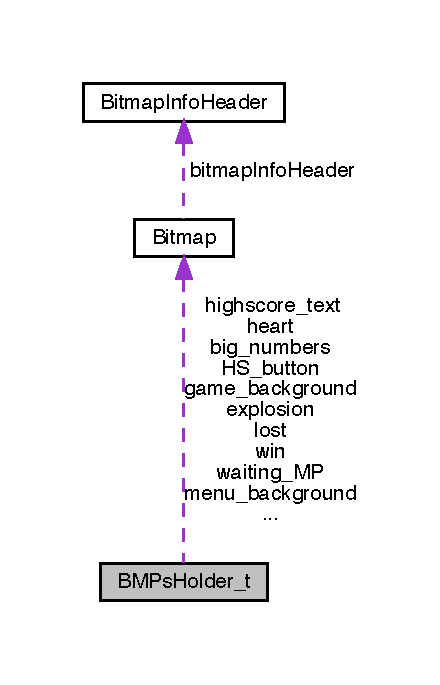
\includegraphics[width=211pt]{struct_b_m_ps_holder__t__coll__graph}
\end{center}
\end{figure}
\subsection*{Public Attributes}
\begin{DoxyCompactItemize}
\item 
\hyperlink{struct_bitmap}{Bitmap} $\ast$$\ast$ \hyperlink{struct_b_m_ps_holder__t_abf522b5ab7fa5ca09282b2b6ce8efe2b}{numbers}
\item 
\hyperlink{struct_bitmap}{Bitmap} $\ast$$\ast$ \hyperlink{struct_b_m_ps_holder__t_a5c1aac4b756c7caaadd1e857cc168c3a}{big\+\_\+numbers}
\begin{DoxyCompactList}\small\item\em \begin{quote}
Array containing the pointers to the numbers bitmaps \end{quote}
\end{DoxyCompactList}\item 
\hyperlink{struct_bitmap}{Bitmap} $\ast$$\ast$ \hyperlink{struct_b_m_ps_holder__t_adf9a39188fb506844694ba403d97e4a1}{explosion}
\begin{DoxyCompactList}\small\item\em \begin{quote}
Array containing the pointers to the big numbers bitmaps \end{quote}
\end{DoxyCompactList}\item 
\hyperlink{struct_bitmap}{Bitmap} $\ast$$\ast$ \hyperlink{struct_b_m_ps_holder__t_a71756da7b641decbe1333acdb01b05ee}{buildings}
\begin{DoxyCompactList}\small\item\em \begin{quote}
Array containing the pointers to the explosion bitmaps \end{quote}
\end{DoxyCompactList}\item 
\hyperlink{struct_bitmap}{Bitmap} $\ast$ \hyperlink{struct_b_m_ps_holder__t_a25d808b859252665b213d2b1430d521a}{game\+\_\+background}
\begin{DoxyCompactList}\small\item\em \begin{quote}
Array containing the pointers to the building destruction bitmaps \end{quote}
\end{DoxyCompactList}\item 
\hyperlink{struct_bitmap}{Bitmap} $\ast$ \hyperlink{struct_b_m_ps_holder__t_a2f28777b77117387410c5e20ff925c44}{H\+S\+\_\+background}
\begin{DoxyCompactList}\small\item\em \begin{quote}
Pointer to the bitmap of the game background \end{quote}
\end{DoxyCompactList}\item 
\hyperlink{struct_bitmap}{Bitmap} $\ast$ \hyperlink{struct_b_m_ps_holder__t_a20a8f018e047cf6d61906b9d11b0a622}{heart}
\begin{DoxyCompactList}\small\item\em \begin{quote}
Pointer to the bitmap of the highscores background \end{quote}
\end{DoxyCompactList}\item 
\hyperlink{struct_bitmap}{Bitmap} $\ast$ \hyperlink{struct_b_m_ps_holder__t_ac193d2d14607ee64994b4385d21808b3}{menu\+\_\+background}
\begin{DoxyCompactList}\small\item\em \begin{quote}
Pointer to the bitmap of the hearts representing the remaining lives of the player \end{quote}
\end{DoxyCompactList}\item 
\hyperlink{struct_bitmap}{Bitmap} $\ast$ \hyperlink{struct_b_m_ps_holder__t_a7f5933cadc7f54074b09ce901893a609}{S\+P\+\_\+button}
\begin{DoxyCompactList}\small\item\em \begin{quote}
Pointer to the bitmap of the menu background \end{quote}
\end{DoxyCompactList}\item 
\hyperlink{struct_bitmap}{Bitmap} $\ast$ \hyperlink{struct_b_m_ps_holder__t_a4c46a999d7b9f15c2ecc0ad5b3b69163}{M\+P\+\_\+button}
\begin{DoxyCompactList}\small\item\em \begin{quote}
Pointer to the bitmap of the single player button \end{quote}
\end{DoxyCompactList}\item 
\hyperlink{struct_bitmap}{Bitmap} $\ast$ \hyperlink{struct_b_m_ps_holder__t_af7900570e309f23ad946097469181db9}{H\+S\+\_\+button}
\begin{DoxyCompactList}\small\item\em \begin{quote}
Pointer to the bitmap of the multi player button \end{quote}
\end{DoxyCompactList}\item 
\hyperlink{struct_bitmap}{Bitmap} $\ast$ \hyperlink{struct_b_m_ps_holder__t_a363b4830dc5cd37d23062b81c64d1903}{highscore\+\_\+text}
\begin{DoxyCompactList}\small\item\em \begin{quote}
Pointer to the bitmap of the highscores button \end{quote}
\end{DoxyCompactList}\item 
\hyperlink{struct_bitmap}{Bitmap} $\ast$ \hyperlink{struct_b_m_ps_holder__t_ac67fdbe89e0f655e44d4445901fb5692}{waiting\+\_\+\+MP}
\begin{DoxyCompactList}\small\item\em \begin{quote}
Pointer to the bitmap of the highscore text showed in the end of a game \end{quote}
\end{DoxyCompactList}\item 
\hyperlink{struct_bitmap}{Bitmap} $\ast$ \hyperlink{struct_b_m_ps_holder__t_a4eee83abbb2345c4be67f06fac361d94}{win}
\begin{DoxyCompactList}\small\item\em \begin{quote}
Pointer to the bitmap showed when waiting for other player (multiplayer mode) \end{quote}
\end{DoxyCompactList}\item 
\hyperlink{struct_bitmap}{Bitmap} $\ast$ \hyperlink{struct_b_m_ps_holder__t_a45ecec1d2762f2fd9f9ccc6ffc0cdbf6}{lost}
\begin{DoxyCompactList}\small\item\em \begin{quote}
Pointer to the \hyperlink{struct_bitmap}{Bitmap} showed when user won in Multiplayer mode \end{quote}
\end{DoxyCompactList}\end{DoxyCompactItemize}


\subsection{Detailed Description}
A structure created to hold all the Bitmaps used in the game. 

\subsection{Member Data Documentation}
\hypertarget{struct_b_m_ps_holder__t_a5c1aac4b756c7caaadd1e857cc168c3a}{}\label{struct_b_m_ps_holder__t_a5c1aac4b756c7caaadd1e857cc168c3a} 
\index{B\+M\+Ps\+Holder\+\_\+t@{B\+M\+Ps\+Holder\+\_\+t}!big\+\_\+numbers@{big\+\_\+numbers}}
\index{big\+\_\+numbers@{big\+\_\+numbers}!B\+M\+Ps\+Holder\+\_\+t@{B\+M\+Ps\+Holder\+\_\+t}}
\subsubsection{\texorpdfstring{big\+\_\+numbers}{big\_numbers}}
{\footnotesize\ttfamily \hyperlink{struct_bitmap}{Bitmap}$\ast$$\ast$ B\+M\+Ps\+Holder\+\_\+t\+::big\+\_\+numbers}



\begin{quote}
Array containing the pointers to the numbers bitmaps \end{quote}


\hypertarget{struct_b_m_ps_holder__t_a71756da7b641decbe1333acdb01b05ee}{}\label{struct_b_m_ps_holder__t_a71756da7b641decbe1333acdb01b05ee} 
\index{B\+M\+Ps\+Holder\+\_\+t@{B\+M\+Ps\+Holder\+\_\+t}!buildings@{buildings}}
\index{buildings@{buildings}!B\+M\+Ps\+Holder\+\_\+t@{B\+M\+Ps\+Holder\+\_\+t}}
\subsubsection{\texorpdfstring{buildings}{buildings}}
{\footnotesize\ttfamily \hyperlink{struct_bitmap}{Bitmap}$\ast$$\ast$ B\+M\+Ps\+Holder\+\_\+t\+::buildings}



\begin{quote}
Array containing the pointers to the explosion bitmaps \end{quote}


\hypertarget{struct_b_m_ps_holder__t_adf9a39188fb506844694ba403d97e4a1}{}\label{struct_b_m_ps_holder__t_adf9a39188fb506844694ba403d97e4a1} 
\index{B\+M\+Ps\+Holder\+\_\+t@{B\+M\+Ps\+Holder\+\_\+t}!explosion@{explosion}}
\index{explosion@{explosion}!B\+M\+Ps\+Holder\+\_\+t@{B\+M\+Ps\+Holder\+\_\+t}}
\subsubsection{\texorpdfstring{explosion}{explosion}}
{\footnotesize\ttfamily \hyperlink{struct_bitmap}{Bitmap}$\ast$$\ast$ B\+M\+Ps\+Holder\+\_\+t\+::explosion}



\begin{quote}
Array containing the pointers to the big numbers bitmaps \end{quote}


\hypertarget{struct_b_m_ps_holder__t_a25d808b859252665b213d2b1430d521a}{}\label{struct_b_m_ps_holder__t_a25d808b859252665b213d2b1430d521a} 
\index{B\+M\+Ps\+Holder\+\_\+t@{B\+M\+Ps\+Holder\+\_\+t}!game\+\_\+background@{game\+\_\+background}}
\index{game\+\_\+background@{game\+\_\+background}!B\+M\+Ps\+Holder\+\_\+t@{B\+M\+Ps\+Holder\+\_\+t}}
\subsubsection{\texorpdfstring{game\+\_\+background}{game\_background}}
{\footnotesize\ttfamily \hyperlink{struct_bitmap}{Bitmap}$\ast$ B\+M\+Ps\+Holder\+\_\+t\+::game\+\_\+background}



\begin{quote}
Array containing the pointers to the building destruction bitmaps \end{quote}


\hypertarget{struct_b_m_ps_holder__t_a20a8f018e047cf6d61906b9d11b0a622}{}\label{struct_b_m_ps_holder__t_a20a8f018e047cf6d61906b9d11b0a622} 
\index{B\+M\+Ps\+Holder\+\_\+t@{B\+M\+Ps\+Holder\+\_\+t}!heart@{heart}}
\index{heart@{heart}!B\+M\+Ps\+Holder\+\_\+t@{B\+M\+Ps\+Holder\+\_\+t}}
\subsubsection{\texorpdfstring{heart}{heart}}
{\footnotesize\ttfamily \hyperlink{struct_bitmap}{Bitmap}$\ast$ B\+M\+Ps\+Holder\+\_\+t\+::heart}



\begin{quote}
Pointer to the bitmap of the highscores background \end{quote}


\hypertarget{struct_b_m_ps_holder__t_a363b4830dc5cd37d23062b81c64d1903}{}\label{struct_b_m_ps_holder__t_a363b4830dc5cd37d23062b81c64d1903} 
\index{B\+M\+Ps\+Holder\+\_\+t@{B\+M\+Ps\+Holder\+\_\+t}!highscore\+\_\+text@{highscore\+\_\+text}}
\index{highscore\+\_\+text@{highscore\+\_\+text}!B\+M\+Ps\+Holder\+\_\+t@{B\+M\+Ps\+Holder\+\_\+t}}
\subsubsection{\texorpdfstring{highscore\+\_\+text}{highscore\_text}}
{\footnotesize\ttfamily \hyperlink{struct_bitmap}{Bitmap}$\ast$ B\+M\+Ps\+Holder\+\_\+t\+::highscore\+\_\+text}



\begin{quote}
Pointer to the bitmap of the highscores button \end{quote}


\hypertarget{struct_b_m_ps_holder__t_a2f28777b77117387410c5e20ff925c44}{}\label{struct_b_m_ps_holder__t_a2f28777b77117387410c5e20ff925c44} 
\index{B\+M\+Ps\+Holder\+\_\+t@{B\+M\+Ps\+Holder\+\_\+t}!H\+S\+\_\+background@{H\+S\+\_\+background}}
\index{H\+S\+\_\+background@{H\+S\+\_\+background}!B\+M\+Ps\+Holder\+\_\+t@{B\+M\+Ps\+Holder\+\_\+t}}
\subsubsection{\texorpdfstring{H\+S\+\_\+background}{HS\_background}}
{\footnotesize\ttfamily \hyperlink{struct_bitmap}{Bitmap}$\ast$ B\+M\+Ps\+Holder\+\_\+t\+::\+H\+S\+\_\+background}



\begin{quote}
Pointer to the bitmap of the game background \end{quote}


\hypertarget{struct_b_m_ps_holder__t_af7900570e309f23ad946097469181db9}{}\label{struct_b_m_ps_holder__t_af7900570e309f23ad946097469181db9} 
\index{B\+M\+Ps\+Holder\+\_\+t@{B\+M\+Ps\+Holder\+\_\+t}!H\+S\+\_\+button@{H\+S\+\_\+button}}
\index{H\+S\+\_\+button@{H\+S\+\_\+button}!B\+M\+Ps\+Holder\+\_\+t@{B\+M\+Ps\+Holder\+\_\+t}}
\subsubsection{\texorpdfstring{H\+S\+\_\+button}{HS\_button}}
{\footnotesize\ttfamily \hyperlink{struct_bitmap}{Bitmap}$\ast$ B\+M\+Ps\+Holder\+\_\+t\+::\+H\+S\+\_\+button}



\begin{quote}
Pointer to the bitmap of the multi player button \end{quote}


\hypertarget{struct_b_m_ps_holder__t_a45ecec1d2762f2fd9f9ccc6ffc0cdbf6}{}\label{struct_b_m_ps_holder__t_a45ecec1d2762f2fd9f9ccc6ffc0cdbf6} 
\index{B\+M\+Ps\+Holder\+\_\+t@{B\+M\+Ps\+Holder\+\_\+t}!lost@{lost}}
\index{lost@{lost}!B\+M\+Ps\+Holder\+\_\+t@{B\+M\+Ps\+Holder\+\_\+t}}
\subsubsection{\texorpdfstring{lost}{lost}}
{\footnotesize\ttfamily \hyperlink{struct_bitmap}{Bitmap}$\ast$ B\+M\+Ps\+Holder\+\_\+t\+::lost}



\begin{quote}
Pointer to the \hyperlink{struct_bitmap}{Bitmap} showed when user won in Multiplayer mode \end{quote}


\hypertarget{struct_b_m_ps_holder__t_ac193d2d14607ee64994b4385d21808b3}{}\label{struct_b_m_ps_holder__t_ac193d2d14607ee64994b4385d21808b3} 
\index{B\+M\+Ps\+Holder\+\_\+t@{B\+M\+Ps\+Holder\+\_\+t}!menu\+\_\+background@{menu\+\_\+background}}
\index{menu\+\_\+background@{menu\+\_\+background}!B\+M\+Ps\+Holder\+\_\+t@{B\+M\+Ps\+Holder\+\_\+t}}
\subsubsection{\texorpdfstring{menu\+\_\+background}{menu\_background}}
{\footnotesize\ttfamily \hyperlink{struct_bitmap}{Bitmap}$\ast$ B\+M\+Ps\+Holder\+\_\+t\+::menu\+\_\+background}



\begin{quote}
Pointer to the bitmap of the hearts representing the remaining lives of the player \end{quote}


\hypertarget{struct_b_m_ps_holder__t_a4c46a999d7b9f15c2ecc0ad5b3b69163}{}\label{struct_b_m_ps_holder__t_a4c46a999d7b9f15c2ecc0ad5b3b69163} 
\index{B\+M\+Ps\+Holder\+\_\+t@{B\+M\+Ps\+Holder\+\_\+t}!M\+P\+\_\+button@{M\+P\+\_\+button}}
\index{M\+P\+\_\+button@{M\+P\+\_\+button}!B\+M\+Ps\+Holder\+\_\+t@{B\+M\+Ps\+Holder\+\_\+t}}
\subsubsection{\texorpdfstring{M\+P\+\_\+button}{MP\_button}}
{\footnotesize\ttfamily \hyperlink{struct_bitmap}{Bitmap}$\ast$ B\+M\+Ps\+Holder\+\_\+t\+::\+M\+P\+\_\+button}



\begin{quote}
Pointer to the bitmap of the single player button \end{quote}


\hypertarget{struct_b_m_ps_holder__t_abf522b5ab7fa5ca09282b2b6ce8efe2b}{}\label{struct_b_m_ps_holder__t_abf522b5ab7fa5ca09282b2b6ce8efe2b} 
\index{B\+M\+Ps\+Holder\+\_\+t@{B\+M\+Ps\+Holder\+\_\+t}!numbers@{numbers}}
\index{numbers@{numbers}!B\+M\+Ps\+Holder\+\_\+t@{B\+M\+Ps\+Holder\+\_\+t}}
\subsubsection{\texorpdfstring{numbers}{numbers}}
{\footnotesize\ttfamily \hyperlink{struct_bitmap}{Bitmap}$\ast$$\ast$ B\+M\+Ps\+Holder\+\_\+t\+::numbers}

\hypertarget{struct_b_m_ps_holder__t_a7f5933cadc7f54074b09ce901893a609}{}\label{struct_b_m_ps_holder__t_a7f5933cadc7f54074b09ce901893a609} 
\index{B\+M\+Ps\+Holder\+\_\+t@{B\+M\+Ps\+Holder\+\_\+t}!S\+P\+\_\+button@{S\+P\+\_\+button}}
\index{S\+P\+\_\+button@{S\+P\+\_\+button}!B\+M\+Ps\+Holder\+\_\+t@{B\+M\+Ps\+Holder\+\_\+t}}
\subsubsection{\texorpdfstring{S\+P\+\_\+button}{SP\_button}}
{\footnotesize\ttfamily \hyperlink{struct_bitmap}{Bitmap}$\ast$ B\+M\+Ps\+Holder\+\_\+t\+::\+S\+P\+\_\+button}



\begin{quote}
Pointer to the bitmap of the menu background \end{quote}


\hypertarget{struct_b_m_ps_holder__t_ac67fdbe89e0f655e44d4445901fb5692}{}\label{struct_b_m_ps_holder__t_ac67fdbe89e0f655e44d4445901fb5692} 
\index{B\+M\+Ps\+Holder\+\_\+t@{B\+M\+Ps\+Holder\+\_\+t}!waiting\+\_\+\+MP@{waiting\+\_\+\+MP}}
\index{waiting\+\_\+\+MP@{waiting\+\_\+\+MP}!B\+M\+Ps\+Holder\+\_\+t@{B\+M\+Ps\+Holder\+\_\+t}}
\subsubsection{\texorpdfstring{waiting\+\_\+\+MP}{waiting\_MP}}
{\footnotesize\ttfamily \hyperlink{struct_bitmap}{Bitmap}$\ast$ B\+M\+Ps\+Holder\+\_\+t\+::waiting\+\_\+\+MP}



\begin{quote}
Pointer to the bitmap of the highscore text showed in the end of a game \end{quote}


\hypertarget{struct_b_m_ps_holder__t_a4eee83abbb2345c4be67f06fac361d94}{}\label{struct_b_m_ps_holder__t_a4eee83abbb2345c4be67f06fac361d94} 
\index{B\+M\+Ps\+Holder\+\_\+t@{B\+M\+Ps\+Holder\+\_\+t}!win@{win}}
\index{win@{win}!B\+M\+Ps\+Holder\+\_\+t@{B\+M\+Ps\+Holder\+\_\+t}}
\subsubsection{\texorpdfstring{win}{win}}
{\footnotesize\ttfamily \hyperlink{struct_bitmap}{Bitmap}$\ast$ B\+M\+Ps\+Holder\+\_\+t\+::win}



\begin{quote}
Pointer to the bitmap showed when waiting for other player (multiplayer mode) \end{quote}




The documentation for this struct was generated from the following file\+:\begin{DoxyCompactItemize}
\item 
/\+Users/andre/\+Documents/lcom1617-\/t4g01/proj/src/\hyperlink{_b_m_ps_holder_8h}{B\+M\+Ps\+Holder.\+h}\end{DoxyCompactItemize}

\hypertarget{struct_date__t}{}\section{Date\+\_\+t Struct Reference}
\label{struct_date__t}\index{Date\+\_\+t@{Date\+\_\+t}}


Structure used to save a date.  




{\ttfamily \#include $<$R\+T\+C.\+h$>$}

\subsection*{Public Attributes}
\begin{DoxyCompactItemize}
\item 
unsigned long \hyperlink{struct_date__t_a6229b5d29374950a2304217dda206f3e}{minute}
\item 
unsigned long \hyperlink{struct_date__t_a7fee0e3c9e76065caa6bf859e3a351ea}{hour}
\begin{DoxyCompactList}\small\item\em \begin{quote}
Minute of the date \end{quote}
\end{DoxyCompactList}\item 
unsigned long \hyperlink{struct_date__t_a270823800a62aa498b9555c99769a3b5}{day}
\begin{DoxyCompactList}\small\item\em \begin{quote}
Hour of the date \end{quote}
\end{DoxyCompactList}\item 
unsigned long \hyperlink{struct_date__t_a2ee23f8b842ac810439f48929dc02d0a}{month}
\begin{DoxyCompactList}\small\item\em \begin{quote}
Day of the date \end{quote}
\end{DoxyCompactList}\item 
unsigned long \hyperlink{struct_date__t_af593228c5b6e2316a755c061bbea3d34}{year}
\begin{DoxyCompactList}\small\item\em \begin{quote}
Month of the date \end{quote}
\end{DoxyCompactList}\end{DoxyCompactItemize}


\subsection{Detailed Description}
Structure used to save a date. 

\subsection{Member Data Documentation}
\hypertarget{struct_date__t_a270823800a62aa498b9555c99769a3b5}{}\label{struct_date__t_a270823800a62aa498b9555c99769a3b5} 
\index{Date\+\_\+t@{Date\+\_\+t}!day@{day}}
\index{day@{day}!Date\+\_\+t@{Date\+\_\+t}}
\subsubsection{\texorpdfstring{day}{day}}
{\footnotesize\ttfamily unsigned long Date\+\_\+t\+::day}



\begin{quote}
Hour of the date \end{quote}


\hypertarget{struct_date__t_a7fee0e3c9e76065caa6bf859e3a351ea}{}\label{struct_date__t_a7fee0e3c9e76065caa6bf859e3a351ea} 
\index{Date\+\_\+t@{Date\+\_\+t}!hour@{hour}}
\index{hour@{hour}!Date\+\_\+t@{Date\+\_\+t}}
\subsubsection{\texorpdfstring{hour}{hour}}
{\footnotesize\ttfamily unsigned long Date\+\_\+t\+::hour}



\begin{quote}
Minute of the date \end{quote}


\hypertarget{struct_date__t_a6229b5d29374950a2304217dda206f3e}{}\label{struct_date__t_a6229b5d29374950a2304217dda206f3e} 
\index{Date\+\_\+t@{Date\+\_\+t}!minute@{minute}}
\index{minute@{minute}!Date\+\_\+t@{Date\+\_\+t}}
\subsubsection{\texorpdfstring{minute}{minute}}
{\footnotesize\ttfamily unsigned long Date\+\_\+t\+::minute}

\hypertarget{struct_date__t_a2ee23f8b842ac810439f48929dc02d0a}{}\label{struct_date__t_a2ee23f8b842ac810439f48929dc02d0a} 
\index{Date\+\_\+t@{Date\+\_\+t}!month@{month}}
\index{month@{month}!Date\+\_\+t@{Date\+\_\+t}}
\subsubsection{\texorpdfstring{month}{month}}
{\footnotesize\ttfamily unsigned long Date\+\_\+t\+::month}



\begin{quote}
Day of the date \end{quote}


\hypertarget{struct_date__t_af593228c5b6e2316a755c061bbea3d34}{}\label{struct_date__t_af593228c5b6e2316a755c061bbea3d34} 
\index{Date\+\_\+t@{Date\+\_\+t}!year@{year}}
\index{year@{year}!Date\+\_\+t@{Date\+\_\+t}}
\subsubsection{\texorpdfstring{year}{year}}
{\footnotesize\ttfamily unsigned long Date\+\_\+t\+::year}



\begin{quote}
Month of the date \end{quote}




The documentation for this struct was generated from the following file\+:\begin{DoxyCompactItemize}
\item 
/\+Users/andre/\+Documents/lcom1617-\/t4g01/proj/src/\hyperlink{_r_t_c_8h}{R\+T\+C.\+h}\end{DoxyCompactItemize}

\hypertarget{structexplosion__t}{}\section{explosion\+\_\+t Struct Reference}
\label{structexplosion__t}\index{explosion\+\_\+t@{explosion\+\_\+t}}


Collaboration diagram for explosion\+\_\+t\+:\nopagebreak
\begin{figure}[H]
\begin{center}
\leavevmode
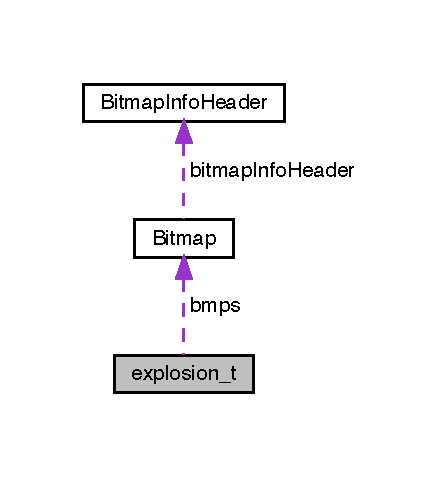
\includegraphics[width=211pt]{structexplosion__t__coll__graph}
\end{center}
\end{figure}
\subsection*{Public Attributes}
\begin{DoxyCompactItemize}
\item 
int \hyperlink{structexplosion__t_a75cfb98cbaf58d5050310154d9acd899}{pos} \mbox{[}2\mbox{]}
\item 
int \hyperlink{structexplosion__t_a1a6cee063c004b26862a9bfefb443d9d}{radius}
\begin{DoxyCompactList}\small\item\em \begin{quote}
Center position of Explosion (x,y) \end{quote}
\end{DoxyCompactList}\item 
\hyperlink{struct_bitmap}{Bitmap} $\ast$$\ast$ \hyperlink{structexplosion__t_ac70416c24cbc420b431ca0ae420e3c56}{bmps}
\begin{DoxyCompactList}\small\item\em \begin{quote}
Radius of Explosion \end{quote}
\end{DoxyCompactList}\item 
unsigned \hyperlink{structexplosion__t_ada685f079492730e96d875d5d8d4d6f9}{curr\+\_\+bmp\+\_\+index}
\begin{DoxyCompactList}\small\item\em \begin{quote}
Explosion Animation \end{quote}
\end{DoxyCompactList}\item 
unsigned \hyperlink{structexplosion__t_a2f8ea40859d72273c6832774e9c501ed}{no\+\_\+bmps}
\begin{DoxyCompactList}\small\item\em \begin{quote}
current bitmap being displayed \end{quote}
\end{DoxyCompactList}\item 
unsigned \hyperlink{structexplosion__t_a84bc7211fa4f7cca4841b6a43e2404d0}{frame\+\_\+count}
\begin{DoxyCompactList}\small\item\em \begin{quote}
Explosion ended \end{quote}
\end{DoxyCompactList}\item 
unsigned \hyperlink{structexplosion__t_a2793afa1a8a4c984dd1d3ac5b4cb1eba}{frames\+\_\+per\+\_\+bmp}
\end{DoxyCompactItemize}


\subsection{Detailed Description}
Structure used to define explosions 

\subsection{Member Data Documentation}
\hypertarget{structexplosion__t_ac70416c24cbc420b431ca0ae420e3c56}{}\label{structexplosion__t_ac70416c24cbc420b431ca0ae420e3c56} 
\index{explosion\+\_\+t@{explosion\+\_\+t}!bmps@{bmps}}
\index{bmps@{bmps}!explosion\+\_\+t@{explosion\+\_\+t}}
\subsubsection{\texorpdfstring{bmps}{bmps}}
{\footnotesize\ttfamily \hyperlink{struct_bitmap}{Bitmap}$\ast$$\ast$ explosion\+\_\+t\+::bmps}



\begin{quote}
Radius of Explosion \end{quote}


\hypertarget{structexplosion__t_ada685f079492730e96d875d5d8d4d6f9}{}\label{structexplosion__t_ada685f079492730e96d875d5d8d4d6f9} 
\index{explosion\+\_\+t@{explosion\+\_\+t}!curr\+\_\+bmp\+\_\+index@{curr\+\_\+bmp\+\_\+index}}
\index{curr\+\_\+bmp\+\_\+index@{curr\+\_\+bmp\+\_\+index}!explosion\+\_\+t@{explosion\+\_\+t}}
\subsubsection{\texorpdfstring{curr\+\_\+bmp\+\_\+index}{curr\_bmp\_index}}
{\footnotesize\ttfamily unsigned explosion\+\_\+t\+::curr\+\_\+bmp\+\_\+index}



\begin{quote}
Explosion Animation \end{quote}


\hypertarget{structexplosion__t_a84bc7211fa4f7cca4841b6a43e2404d0}{}\label{structexplosion__t_a84bc7211fa4f7cca4841b6a43e2404d0} 
\index{explosion\+\_\+t@{explosion\+\_\+t}!frame\+\_\+count@{frame\+\_\+count}}
\index{frame\+\_\+count@{frame\+\_\+count}!explosion\+\_\+t@{explosion\+\_\+t}}
\subsubsection{\texorpdfstring{frame\+\_\+count}{frame\_count}}
{\footnotesize\ttfamily unsigned explosion\+\_\+t\+::frame\+\_\+count}



\begin{quote}
Explosion ended \end{quote}


\hypertarget{structexplosion__t_a2793afa1a8a4c984dd1d3ac5b4cb1eba}{}\label{structexplosion__t_a2793afa1a8a4c984dd1d3ac5b4cb1eba} 
\index{explosion\+\_\+t@{explosion\+\_\+t}!frames\+\_\+per\+\_\+bmp@{frames\+\_\+per\+\_\+bmp}}
\index{frames\+\_\+per\+\_\+bmp@{frames\+\_\+per\+\_\+bmp}!explosion\+\_\+t@{explosion\+\_\+t}}
\subsubsection{\texorpdfstring{frames\+\_\+per\+\_\+bmp}{frames\_per\_bmp}}
{\footnotesize\ttfamily unsigned explosion\+\_\+t\+::frames\+\_\+per\+\_\+bmp}

\hypertarget{structexplosion__t_a2f8ea40859d72273c6832774e9c501ed}{}\label{structexplosion__t_a2f8ea40859d72273c6832774e9c501ed} 
\index{explosion\+\_\+t@{explosion\+\_\+t}!no\+\_\+bmps@{no\+\_\+bmps}}
\index{no\+\_\+bmps@{no\+\_\+bmps}!explosion\+\_\+t@{explosion\+\_\+t}}
\subsubsection{\texorpdfstring{no\+\_\+bmps}{no\_bmps}}
{\footnotesize\ttfamily unsigned explosion\+\_\+t\+::no\+\_\+bmps}



\begin{quote}
current bitmap being displayed \end{quote}


\hypertarget{structexplosion__t_a75cfb98cbaf58d5050310154d9acd899}{}\label{structexplosion__t_a75cfb98cbaf58d5050310154d9acd899} 
\index{explosion\+\_\+t@{explosion\+\_\+t}!pos@{pos}}
\index{pos@{pos}!explosion\+\_\+t@{explosion\+\_\+t}}
\subsubsection{\texorpdfstring{pos}{pos}}
{\footnotesize\ttfamily int explosion\+\_\+t\+::pos\mbox{[}2\mbox{]}}

\hypertarget{structexplosion__t_a1a6cee063c004b26862a9bfefb443d9d}{}\label{structexplosion__t_a1a6cee063c004b26862a9bfefb443d9d} 
\index{explosion\+\_\+t@{explosion\+\_\+t}!radius@{radius}}
\index{radius@{radius}!explosion\+\_\+t@{explosion\+\_\+t}}
\subsubsection{\texorpdfstring{radius}{radius}}
{\footnotesize\ttfamily int explosion\+\_\+t\+::radius}



\begin{quote}
Center position of Explosion (x,y) \end{quote}




The documentation for this struct was generated from the following file\+:\begin{DoxyCompactItemize}
\item 
/\+Users/andre/\+Documents/lcom1617-\/t4g01/proj/src/\hyperlink{_missile_8c}{Missile.\+c}\end{DoxyCompactItemize}

\hypertarget{struct_game__t}{}\section{Game\+\_\+t Struct Reference}
\label{struct_game__t}\index{Game\+\_\+t@{Game\+\_\+t}}


Collaboration diagram for Game\+\_\+t\+:\nopagebreak
\begin{figure}[H]
\begin{center}
\leavevmode
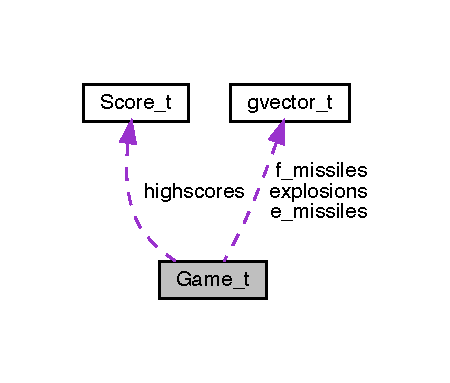
\includegraphics[width=216pt]{struct_game__t__coll__graph}
\end{center}
\end{figure}
\subsection*{Public Attributes}
\begin{DoxyCompactItemize}
\item 
\hyperlink{group___g_vector_ga6d90d5e6b721779a43354f2752b79281}{G\+Vector} $\ast$ \hyperlink{struct_game__t_a30c32876ba91964b9b7083ef244815e9}{e\+\_\+missiles}
\item 
\hyperlink{group___g_vector_ga6d90d5e6b721779a43354f2752b79281}{G\+Vector} $\ast$ \hyperlink{struct_game__t_a9aea8f7d5e9730e64878d220814cf5ee}{f\+\_\+missiles}
\item 
\hyperlink{group___g_vector_ga6d90d5e6b721779a43354f2752b79281}{G\+Vector} $\ast$ \hyperlink{struct_game__t_a14d975d4e5ce1bf613317321e5d43029}{explosions}
\item 
unsigned long \hyperlink{struct_game__t_af4d5f8a155f90b1f37e63d35db44734a}{frames}
\item 
unsigned long \hyperlink{struct_game__t_a2208b5a6b7e8ad55bd0f4e09730d9599}{enemy\+\_\+spawn\+\_\+fr}
\item 
unsigned \hyperlink{struct_game__t_a3d8925453d2141ee634a3bb32e7fc4bf}{cannon\+\_\+pos} \mbox{[}2\mbox{]}
\item 
unsigned \hyperlink{struct_game__t_a172b6aea1411a491f1b6fba4ae7b802b}{health\+\_\+points}
\item 
unsigned \hyperlink{struct_game__t_a210bd36fda417d2fc1356e7f0242c6a2}{bases\+\_\+hp} \mbox{[}3\mbox{]}
\item 
unsigned \hyperlink{struct_game__t_aa3465afd0a5082a9b40aec2f6643bf4a}{bases\+\_\+pos} \mbox{[}3\mbox{]}
\item 
unsigned \hyperlink{struct_game__t_a9cc316346c6e425c84857c694adaedb2}{buildings\+\_\+size\+\_\+y} \mbox{[}3\mbox{]}
\item 
\hyperlink{struct_score__t}{Score\+\_\+t} $\ast$ \hyperlink{struct_game__t_a375852aa9a12c33759d6ab7784fa7314}{highscores}
\end{DoxyCompactItemize}


\subsection{Detailed Description}
Game Struct and Methods 

\subsection{Member Data Documentation}
\hypertarget{struct_game__t_a210bd36fda417d2fc1356e7f0242c6a2}{}\label{struct_game__t_a210bd36fda417d2fc1356e7f0242c6a2} 
\index{Game\+\_\+t@{Game\+\_\+t}!bases\+\_\+hp@{bases\+\_\+hp}}
\index{bases\+\_\+hp@{bases\+\_\+hp}!Game\+\_\+t@{Game\+\_\+t}}
\subsubsection{\texorpdfstring{bases\+\_\+hp}{bases\_hp}}
{\footnotesize\ttfamily unsigned Game\+\_\+t\+::bases\+\_\+hp\mbox{[}3\mbox{]}}

\hypertarget{struct_game__t_aa3465afd0a5082a9b40aec2f6643bf4a}{}\label{struct_game__t_aa3465afd0a5082a9b40aec2f6643bf4a} 
\index{Game\+\_\+t@{Game\+\_\+t}!bases\+\_\+pos@{bases\+\_\+pos}}
\index{bases\+\_\+pos@{bases\+\_\+pos}!Game\+\_\+t@{Game\+\_\+t}}
\subsubsection{\texorpdfstring{bases\+\_\+pos}{bases\_pos}}
{\footnotesize\ttfamily unsigned Game\+\_\+t\+::bases\+\_\+pos\mbox{[}3\mbox{]}}

\hypertarget{struct_game__t_a9cc316346c6e425c84857c694adaedb2}{}\label{struct_game__t_a9cc316346c6e425c84857c694adaedb2} 
\index{Game\+\_\+t@{Game\+\_\+t}!buildings\+\_\+size\+\_\+y@{buildings\+\_\+size\+\_\+y}}
\index{buildings\+\_\+size\+\_\+y@{buildings\+\_\+size\+\_\+y}!Game\+\_\+t@{Game\+\_\+t}}
\subsubsection{\texorpdfstring{buildings\+\_\+size\+\_\+y}{buildings\_size\_y}}
{\footnotesize\ttfamily unsigned Game\+\_\+t\+::buildings\+\_\+size\+\_\+y\mbox{[}3\mbox{]}}

\hypertarget{struct_game__t_a3d8925453d2141ee634a3bb32e7fc4bf}{}\label{struct_game__t_a3d8925453d2141ee634a3bb32e7fc4bf} 
\index{Game\+\_\+t@{Game\+\_\+t}!cannon\+\_\+pos@{cannon\+\_\+pos}}
\index{cannon\+\_\+pos@{cannon\+\_\+pos}!Game\+\_\+t@{Game\+\_\+t}}
\subsubsection{\texorpdfstring{cannon\+\_\+pos}{cannon\_pos}}
{\footnotesize\ttfamily unsigned Game\+\_\+t\+::cannon\+\_\+pos\mbox{[}2\mbox{]}}

\hypertarget{struct_game__t_a30c32876ba91964b9b7083ef244815e9}{}\label{struct_game__t_a30c32876ba91964b9b7083ef244815e9} 
\index{Game\+\_\+t@{Game\+\_\+t}!e\+\_\+missiles@{e\+\_\+missiles}}
\index{e\+\_\+missiles@{e\+\_\+missiles}!Game\+\_\+t@{Game\+\_\+t}}
\subsubsection{\texorpdfstring{e\+\_\+missiles}{e\_missiles}}
{\footnotesize\ttfamily \hyperlink{group___g_vector_ga6d90d5e6b721779a43354f2752b79281}{G\+Vector}$\ast$ Game\+\_\+t\+::e\+\_\+missiles}

\hypertarget{struct_game__t_a2208b5a6b7e8ad55bd0f4e09730d9599}{}\label{struct_game__t_a2208b5a6b7e8ad55bd0f4e09730d9599} 
\index{Game\+\_\+t@{Game\+\_\+t}!enemy\+\_\+spawn\+\_\+fr@{enemy\+\_\+spawn\+\_\+fr}}
\index{enemy\+\_\+spawn\+\_\+fr@{enemy\+\_\+spawn\+\_\+fr}!Game\+\_\+t@{Game\+\_\+t}}
\subsubsection{\texorpdfstring{enemy\+\_\+spawn\+\_\+fr}{enemy\_spawn\_fr}}
{\footnotesize\ttfamily unsigned long Game\+\_\+t\+::enemy\+\_\+spawn\+\_\+fr}

\hypertarget{struct_game__t_a14d975d4e5ce1bf613317321e5d43029}{}\label{struct_game__t_a14d975d4e5ce1bf613317321e5d43029} 
\index{Game\+\_\+t@{Game\+\_\+t}!explosions@{explosions}}
\index{explosions@{explosions}!Game\+\_\+t@{Game\+\_\+t}}
\subsubsection{\texorpdfstring{explosions}{explosions}}
{\footnotesize\ttfamily \hyperlink{group___g_vector_ga6d90d5e6b721779a43354f2752b79281}{G\+Vector}$\ast$ Game\+\_\+t\+::explosions}

\hypertarget{struct_game__t_a9aea8f7d5e9730e64878d220814cf5ee}{}\label{struct_game__t_a9aea8f7d5e9730e64878d220814cf5ee} 
\index{Game\+\_\+t@{Game\+\_\+t}!f\+\_\+missiles@{f\+\_\+missiles}}
\index{f\+\_\+missiles@{f\+\_\+missiles}!Game\+\_\+t@{Game\+\_\+t}}
\subsubsection{\texorpdfstring{f\+\_\+missiles}{f\_missiles}}
{\footnotesize\ttfamily \hyperlink{group___g_vector_ga6d90d5e6b721779a43354f2752b79281}{G\+Vector}$\ast$ Game\+\_\+t\+::f\+\_\+missiles}

\hypertarget{struct_game__t_af4d5f8a155f90b1f37e63d35db44734a}{}\label{struct_game__t_af4d5f8a155f90b1f37e63d35db44734a} 
\index{Game\+\_\+t@{Game\+\_\+t}!frames@{frames}}
\index{frames@{frames}!Game\+\_\+t@{Game\+\_\+t}}
\subsubsection{\texorpdfstring{frames}{frames}}
{\footnotesize\ttfamily unsigned long Game\+\_\+t\+::frames}

\hypertarget{struct_game__t_a172b6aea1411a491f1b6fba4ae7b802b}{}\label{struct_game__t_a172b6aea1411a491f1b6fba4ae7b802b} 
\index{Game\+\_\+t@{Game\+\_\+t}!health\+\_\+points@{health\+\_\+points}}
\index{health\+\_\+points@{health\+\_\+points}!Game\+\_\+t@{Game\+\_\+t}}
\subsubsection{\texorpdfstring{health\+\_\+points}{health\_points}}
{\footnotesize\ttfamily unsigned Game\+\_\+t\+::health\+\_\+points}

\hypertarget{struct_game__t_a375852aa9a12c33759d6ab7784fa7314}{}\label{struct_game__t_a375852aa9a12c33759d6ab7784fa7314} 
\index{Game\+\_\+t@{Game\+\_\+t}!highscores@{highscores}}
\index{highscores@{highscores}!Game\+\_\+t@{Game\+\_\+t}}
\subsubsection{\texorpdfstring{highscores}{highscores}}
{\footnotesize\ttfamily \hyperlink{struct_score__t}{Score\+\_\+t}$\ast$ Game\+\_\+t\+::highscores}



The documentation for this struct was generated from the following file\+:\begin{DoxyCompactItemize}
\item 
/\+Users/andre/\+Documents/lcom1617-\/t4g01/proj/src/\hyperlink{planetary_8c}{planetary.\+c}\end{DoxyCompactItemize}

\hypertarget{structgvector__t}{}\section{gvector\+\_\+t Struct Reference}
\label{structgvector__t}\index{gvector\+\_\+t@{gvector\+\_\+t}}
\subsection*{Public Attributes}
\begin{DoxyCompactItemize}
\item 
unsigned \hyperlink{structgvector__t_a740303b1753b7d95a89c75637c875ca4}{size}
\item 
unsigned \hyperlink{structgvector__t_a535f3426a6ac2dd946d90353674ec8c8}{el\+\_\+size}
\item 
unsigned \hyperlink{structgvector__t_a517503cade4866c47d4de67bb24440d3}{capacity}
\item 
unsigned \hyperlink{structgvector__t_a39ed5cd080d8b5557cd6967c0aae966b}{increments}
\item 
void $\ast$ \hyperlink{structgvector__t_a3bbc50d85feec3c63a31b0ac665fe623}{array}
\end{DoxyCompactItemize}


\subsection{Member Data Documentation}
\hypertarget{structgvector__t_a3bbc50d85feec3c63a31b0ac665fe623}{}\label{structgvector__t_a3bbc50d85feec3c63a31b0ac665fe623} 
\index{gvector\+\_\+t@{gvector\+\_\+t}!array@{array}}
\index{array@{array}!gvector\+\_\+t@{gvector\+\_\+t}}
\subsubsection{\texorpdfstring{array}{array}}
{\footnotesize\ttfamily void$\ast$ gvector\+\_\+t\+::array}

\hypertarget{structgvector__t_a517503cade4866c47d4de67bb24440d3}{}\label{structgvector__t_a517503cade4866c47d4de67bb24440d3} 
\index{gvector\+\_\+t@{gvector\+\_\+t}!capacity@{capacity}}
\index{capacity@{capacity}!gvector\+\_\+t@{gvector\+\_\+t}}
\subsubsection{\texorpdfstring{capacity}{capacity}}
{\footnotesize\ttfamily unsigned gvector\+\_\+t\+::capacity}

\hypertarget{structgvector__t_a535f3426a6ac2dd946d90353674ec8c8}{}\label{structgvector__t_a535f3426a6ac2dd946d90353674ec8c8} 
\index{gvector\+\_\+t@{gvector\+\_\+t}!el\+\_\+size@{el\+\_\+size}}
\index{el\+\_\+size@{el\+\_\+size}!gvector\+\_\+t@{gvector\+\_\+t}}
\subsubsection{\texorpdfstring{el\+\_\+size}{el\_size}}
{\footnotesize\ttfamily unsigned gvector\+\_\+t\+::el\+\_\+size}

\hypertarget{structgvector__t_a39ed5cd080d8b5557cd6967c0aae966b}{}\label{structgvector__t_a39ed5cd080d8b5557cd6967c0aae966b} 
\index{gvector\+\_\+t@{gvector\+\_\+t}!increments@{increments}}
\index{increments@{increments}!gvector\+\_\+t@{gvector\+\_\+t}}
\subsubsection{\texorpdfstring{increments}{increments}}
{\footnotesize\ttfamily unsigned gvector\+\_\+t\+::increments}

\hypertarget{structgvector__t_a740303b1753b7d95a89c75637c875ca4}{}\label{structgvector__t_a740303b1753b7d95a89c75637c875ca4} 
\index{gvector\+\_\+t@{gvector\+\_\+t}!size@{size}}
\index{size@{size}!gvector\+\_\+t@{gvector\+\_\+t}}
\subsubsection{\texorpdfstring{size}{size}}
{\footnotesize\ttfamily unsigned gvector\+\_\+t\+::size}



The documentation for this struct was generated from the following file\+:\begin{DoxyCompactItemize}
\item 
/\+Users/andre/\+Documents/lcom1617-\/t4g01/proj/src/\hyperlink{_g_vector_8c}{G\+Vector.\+c}\end{DoxyCompactItemize}

\hypertarget{struct_input__t}{}\section{Input\+\_\+t Struct Reference}
\label{struct_input__t}\index{Input\+\_\+t@{Input\+\_\+t}}


Structure that keeps record of all the user input information.  




{\ttfamily \#include $<$Input.\+h$>$}

\subsection*{Public Attributes}
\begin{DoxyCompactItemize}
\item 
\hyperlink{group___input_ga6e68664bf6d0e0a4dac76a07ae630c52}{keycode\+\_\+t} \hyperlink{struct_input__t_a1664c83ef92405877db0b04d4643a754}{keycode}
\item 
int \hyperlink{struct_input__t_ae9b94c465b22787a021d494d2c57b6d4}{R\+MB}
\begin{DoxyCompactList}\small\item\em \begin{quote}
Current keyboard key \end{quote}
\end{DoxyCompactList}\item 
int \hyperlink{struct_input__t_af71c02dde674d804117e7915929a3e05}{L\+MB}
\begin{DoxyCompactList}\small\item\em \begin{quote}
Flag for Right Mouse Button (pressed or not) \end{quote}
\end{DoxyCompactList}\item 
int \hyperlink{struct_input__t_a39c2b2bb2313e0a3773c2b8cb2bc94c8}{M\+MB}
\begin{DoxyCompactList}\small\item\em \begin{quote}
Flag for Left Mouse Button (pressed or not) \end{quote}
\end{DoxyCompactList}\item 
int \hyperlink{struct_input__t_a9af766f0cb90f3abf804a9203387f932}{mouse\+\_\+pos} \mbox{[}2\mbox{]}
\begin{DoxyCompactList}\small\item\em \begin{quote}
Flag for Middle Mouse Button (pressed or not) \end{quote}
\end{DoxyCompactList}\item 
unsigned \hyperlink{struct_input__t_a0a91455b460723c1fc8fccb30a4021f8}{res} \mbox{[}2\mbox{]}
\begin{DoxyCompactList}\small\item\em \begin{quote}
Current position of the mouse onn screen (x,y) \end{quote}
\end{DoxyCompactList}\end{DoxyCompactItemize}


\subsection{Detailed Description}
Structure that keeps record of all the user input information. 

\subsection{Member Data Documentation}
\hypertarget{struct_input__t_a1664c83ef92405877db0b04d4643a754}{}\label{struct_input__t_a1664c83ef92405877db0b04d4643a754} 
\index{Input\+\_\+t@{Input\+\_\+t}!keycode@{keycode}}
\index{keycode@{keycode}!Input\+\_\+t@{Input\+\_\+t}}
\subsubsection{\texorpdfstring{keycode}{keycode}}
{\footnotesize\ttfamily \hyperlink{group___input_ga6e68664bf6d0e0a4dac76a07ae630c52}{keycode\+\_\+t} Input\+\_\+t\+::keycode}

\hypertarget{struct_input__t_af71c02dde674d804117e7915929a3e05}{}\label{struct_input__t_af71c02dde674d804117e7915929a3e05} 
\index{Input\+\_\+t@{Input\+\_\+t}!L\+MB@{L\+MB}}
\index{L\+MB@{L\+MB}!Input\+\_\+t@{Input\+\_\+t}}
\subsubsection{\texorpdfstring{L\+MB}{LMB}}
{\footnotesize\ttfamily int Input\+\_\+t\+::\+L\+MB}



\begin{quote}
Flag for Right Mouse Button (pressed or not) \end{quote}


\hypertarget{struct_input__t_a39c2b2bb2313e0a3773c2b8cb2bc94c8}{}\label{struct_input__t_a39c2b2bb2313e0a3773c2b8cb2bc94c8} 
\index{Input\+\_\+t@{Input\+\_\+t}!M\+MB@{M\+MB}}
\index{M\+MB@{M\+MB}!Input\+\_\+t@{Input\+\_\+t}}
\subsubsection{\texorpdfstring{M\+MB}{MMB}}
{\footnotesize\ttfamily int Input\+\_\+t\+::\+M\+MB}



\begin{quote}
Flag for Left Mouse Button (pressed or not) \end{quote}


\hypertarget{struct_input__t_a9af766f0cb90f3abf804a9203387f932}{}\label{struct_input__t_a9af766f0cb90f3abf804a9203387f932} 
\index{Input\+\_\+t@{Input\+\_\+t}!mouse\+\_\+pos@{mouse\+\_\+pos}}
\index{mouse\+\_\+pos@{mouse\+\_\+pos}!Input\+\_\+t@{Input\+\_\+t}}
\subsubsection{\texorpdfstring{mouse\+\_\+pos}{mouse\_pos}}
{\footnotesize\ttfamily int Input\+\_\+t\+::mouse\+\_\+pos\mbox{[}2\mbox{]}}



\begin{quote}
Flag for Middle Mouse Button (pressed or not) \end{quote}


\hypertarget{struct_input__t_a0a91455b460723c1fc8fccb30a4021f8}{}\label{struct_input__t_a0a91455b460723c1fc8fccb30a4021f8} 
\index{Input\+\_\+t@{Input\+\_\+t}!res@{res}}
\index{res@{res}!Input\+\_\+t@{Input\+\_\+t}}
\subsubsection{\texorpdfstring{res}{res}}
{\footnotesize\ttfamily unsigned Input\+\_\+t\+::res\mbox{[}2\mbox{]}}



\begin{quote}
Current position of the mouse onn screen (x,y) \end{quote}


\hypertarget{struct_input__t_ae9b94c465b22787a021d494d2c57b6d4}{}\label{struct_input__t_ae9b94c465b22787a021d494d2c57b6d4} 
\index{Input\+\_\+t@{Input\+\_\+t}!R\+MB@{R\+MB}}
\index{R\+MB@{R\+MB}!Input\+\_\+t@{Input\+\_\+t}}
\subsubsection{\texorpdfstring{R\+MB}{RMB}}
{\footnotesize\ttfamily int Input\+\_\+t\+::\+R\+MB}



\begin{quote}
Current keyboard key \end{quote}




The documentation for this struct was generated from the following file\+:\begin{DoxyCompactItemize}
\item 
/\+Users/andre/\+Documents/lcom1617-\/t4g01/proj/src/\hyperlink{_input_8h}{Input.\+h}\end{DoxyCompactItemize}

\hypertarget{struct_menu__t}{}\section{Menu\+\_\+t Struct Reference}
\label{struct_menu__t}\index{Menu\+\_\+t@{Menu\+\_\+t}}
\subsection*{Public Attributes}
\begin{DoxyCompactItemize}
\item 
unsigned \hyperlink{struct_menu__t_a73413f3fc2848f75e731c17a4ba51f74}{S\+P\+\_\+pos} \mbox{[}2\mbox{]}
\item 
unsigned \hyperlink{struct_menu__t_a252b5ddb2d7e97a790ef0a5d95af6078}{M\+P\+\_\+pos} \mbox{[}2\mbox{]}
\item 
unsigned \hyperlink{struct_menu__t_ae3ed027861d6123a178a82a6f60fdb74}{H\+S\+\_\+pos} \mbox{[}2\mbox{]}
\item 
unsigned \hyperlink{struct_menu__t_a7d1e90a9edc6dacce833bb39ab75e1e3}{options\+\_\+size} \mbox{[}2\mbox{]}
\item 
unsigned \hyperlink{struct_menu__t_ad826ecbf028d96d83976029b06fff7fb}{exit\+\_\+pos} \mbox{[}2\mbox{]}
\item 
unsigned \hyperlink{struct_menu__t_a6a89c2eaee92b6c3cc3359088fe6951f}{exit\+\_\+radius}
\end{DoxyCompactItemize}


\subsection{Detailed Description}
Menu Struct and Methods 

\subsection{Member Data Documentation}
\hypertarget{struct_menu__t_ad826ecbf028d96d83976029b06fff7fb}{}\label{struct_menu__t_ad826ecbf028d96d83976029b06fff7fb} 
\index{Menu\+\_\+t@{Menu\+\_\+t}!exit\+\_\+pos@{exit\+\_\+pos}}
\index{exit\+\_\+pos@{exit\+\_\+pos}!Menu\+\_\+t@{Menu\+\_\+t}}
\subsubsection{\texorpdfstring{exit\+\_\+pos}{exit\_pos}}
{\footnotesize\ttfamily unsigned Menu\+\_\+t\+::exit\+\_\+pos\mbox{[}2\mbox{]}}

\hypertarget{struct_menu__t_a6a89c2eaee92b6c3cc3359088fe6951f}{}\label{struct_menu__t_a6a89c2eaee92b6c3cc3359088fe6951f} 
\index{Menu\+\_\+t@{Menu\+\_\+t}!exit\+\_\+radius@{exit\+\_\+radius}}
\index{exit\+\_\+radius@{exit\+\_\+radius}!Menu\+\_\+t@{Menu\+\_\+t}}
\subsubsection{\texorpdfstring{exit\+\_\+radius}{exit\_radius}}
{\footnotesize\ttfamily unsigned Menu\+\_\+t\+::exit\+\_\+radius}

\hypertarget{struct_menu__t_ae3ed027861d6123a178a82a6f60fdb74}{}\label{struct_menu__t_ae3ed027861d6123a178a82a6f60fdb74} 
\index{Menu\+\_\+t@{Menu\+\_\+t}!H\+S\+\_\+pos@{H\+S\+\_\+pos}}
\index{H\+S\+\_\+pos@{H\+S\+\_\+pos}!Menu\+\_\+t@{Menu\+\_\+t}}
\subsubsection{\texorpdfstring{H\+S\+\_\+pos}{HS\_pos}}
{\footnotesize\ttfamily unsigned Menu\+\_\+t\+::\+H\+S\+\_\+pos\mbox{[}2\mbox{]}}

\hypertarget{struct_menu__t_a252b5ddb2d7e97a790ef0a5d95af6078}{}\label{struct_menu__t_a252b5ddb2d7e97a790ef0a5d95af6078} 
\index{Menu\+\_\+t@{Menu\+\_\+t}!M\+P\+\_\+pos@{M\+P\+\_\+pos}}
\index{M\+P\+\_\+pos@{M\+P\+\_\+pos}!Menu\+\_\+t@{Menu\+\_\+t}}
\subsubsection{\texorpdfstring{M\+P\+\_\+pos}{MP\_pos}}
{\footnotesize\ttfamily unsigned Menu\+\_\+t\+::\+M\+P\+\_\+pos\mbox{[}2\mbox{]}}

\hypertarget{struct_menu__t_a7d1e90a9edc6dacce833bb39ab75e1e3}{}\label{struct_menu__t_a7d1e90a9edc6dacce833bb39ab75e1e3} 
\index{Menu\+\_\+t@{Menu\+\_\+t}!options\+\_\+size@{options\+\_\+size}}
\index{options\+\_\+size@{options\+\_\+size}!Menu\+\_\+t@{Menu\+\_\+t}}
\subsubsection{\texorpdfstring{options\+\_\+size}{options\_size}}
{\footnotesize\ttfamily unsigned Menu\+\_\+t\+::options\+\_\+size\mbox{[}2\mbox{]}}

\hypertarget{struct_menu__t_a73413f3fc2848f75e731c17a4ba51f74}{}\label{struct_menu__t_a73413f3fc2848f75e731c17a4ba51f74} 
\index{Menu\+\_\+t@{Menu\+\_\+t}!S\+P\+\_\+pos@{S\+P\+\_\+pos}}
\index{S\+P\+\_\+pos@{S\+P\+\_\+pos}!Menu\+\_\+t@{Menu\+\_\+t}}
\subsubsection{\texorpdfstring{S\+P\+\_\+pos}{SP\_pos}}
{\footnotesize\ttfamily unsigned Menu\+\_\+t\+::\+S\+P\+\_\+pos\mbox{[}2\mbox{]}}



The documentation for this struct was generated from the following file\+:\begin{DoxyCompactItemize}
\item 
/\+Users/andre/\+Documents/lcom1617-\/t4g01/proj/src/\hyperlink{planetary_8c}{planetary.\+c}\end{DoxyCompactItemize}

\hypertarget{structmissile__t}{}\section{missile\+\_\+t Struct Reference}
\label{structmissile__t}\index{missile\+\_\+t@{missile\+\_\+t}}
\subsection*{Public Attributes}
\begin{DoxyCompactItemize}
\item 
int \hyperlink{structmissile__t_ae9b8a60e3fc505cbdc6a73eecec22593}{init\+\_\+pos} \mbox{[}2\mbox{]}
\item 
int \hyperlink{structmissile__t_acad3785ef3162b36ea58106e7cac3d3c}{pos} \mbox{[}2\mbox{]}
\begin{DoxyCompactList}\small\item\em \begin{quote}
Initial Position for Missile Trail \end{quote}
\end{DoxyCompactList}\item 
float \hyperlink{structmissile__t_a33888390438f5edf647bf8ddf7ebd646}{velocity} \mbox{[}2\mbox{]}
\begin{DoxyCompactList}\small\item\em \begin{quote}
Current Position \end{quote}
\end{DoxyCompactList}\item 
float \hyperlink{structmissile__t_ad8c173c28c4adbf4b25292f0d2ea6a82}{pending\+\_\+movement} \mbox{[}2\mbox{]}
\begin{DoxyCompactList}\small\item\em \begin{quote}
Velocity, in pixels P\+ER frame \end{quote}
\end{DoxyCompactList}\item 
uint16\+\_\+t \hyperlink{structmissile__t_ac4f6693bdb22fa048147f089f57c5d59}{color}
\begin{DoxyCompactList}\small\item\em \begin{quote}
Movement left unperformed on the previous frame \end{quote}
\end{DoxyCompactList}\item 
\hyperlink{_missile_8c_af6a258d8f3ee5206d682d799316314b1}{bool} \hyperlink{structmissile__t_a4b5fd447e6a7f348d5986e74d843e8e2}{is\+Friendly}
\begin{DoxyCompactList}\small\item\em \begin{quote}
Color in R\+GB 5\+:6\+:5 \end{quote}
\end{DoxyCompactList}\item 
int \hyperlink{structmissile__t_acfc81d3ad2e8655c604ed499d038256d}{end\+\_\+pos} \mbox{[}2\mbox{]}
\end{DoxyCompactItemize}


\subsection{Detailed Description}
Structure used to define a missile. Common to friendly and enemy missiles. 

\subsection{Member Data Documentation}
\hypertarget{structmissile__t_ac4f6693bdb22fa048147f089f57c5d59}{}\label{structmissile__t_ac4f6693bdb22fa048147f089f57c5d59} 
\index{missile\+\_\+t@{missile\+\_\+t}!color@{color}}
\index{color@{color}!missile\+\_\+t@{missile\+\_\+t}}
\subsubsection{\texorpdfstring{color}{color}}
{\footnotesize\ttfamily uint16\+\_\+t missile\+\_\+t\+::color}



\begin{quote}
Movement left unperformed on the previous frame \end{quote}


\hypertarget{structmissile__t_acfc81d3ad2e8655c604ed499d038256d}{}\label{structmissile__t_acfc81d3ad2e8655c604ed499d038256d} 
\index{missile\+\_\+t@{missile\+\_\+t}!end\+\_\+pos@{end\+\_\+pos}}
\index{end\+\_\+pos@{end\+\_\+pos}!missile\+\_\+t@{missile\+\_\+t}}
\subsubsection{\texorpdfstring{end\+\_\+pos}{end\_pos}}
{\footnotesize\ttfamily int missile\+\_\+t\+::end\+\_\+pos\mbox{[}2\mbox{]}}

\hypertarget{structmissile__t_ae9b8a60e3fc505cbdc6a73eecec22593}{}\label{structmissile__t_ae9b8a60e3fc505cbdc6a73eecec22593} 
\index{missile\+\_\+t@{missile\+\_\+t}!init\+\_\+pos@{init\+\_\+pos}}
\index{init\+\_\+pos@{init\+\_\+pos}!missile\+\_\+t@{missile\+\_\+t}}
\subsubsection{\texorpdfstring{init\+\_\+pos}{init\_pos}}
{\footnotesize\ttfamily int missile\+\_\+t\+::init\+\_\+pos\mbox{[}2\mbox{]}}

\hypertarget{structmissile__t_a4b5fd447e6a7f348d5986e74d843e8e2}{}\label{structmissile__t_a4b5fd447e6a7f348d5986e74d843e8e2} 
\index{missile\+\_\+t@{missile\+\_\+t}!is\+Friendly@{is\+Friendly}}
\index{is\+Friendly@{is\+Friendly}!missile\+\_\+t@{missile\+\_\+t}}
\subsubsection{\texorpdfstring{is\+Friendly}{isFriendly}}
{\footnotesize\ttfamily \hyperlink{_missile_8c_af6a258d8f3ee5206d682d799316314b1}{bool} missile\+\_\+t\+::is\+Friendly}



\begin{quote}
Color in R\+GB 5\+:6\+:5 \end{quote}


\hypertarget{structmissile__t_ad8c173c28c4adbf4b25292f0d2ea6a82}{}\label{structmissile__t_ad8c173c28c4adbf4b25292f0d2ea6a82} 
\index{missile\+\_\+t@{missile\+\_\+t}!pending\+\_\+movement@{pending\+\_\+movement}}
\index{pending\+\_\+movement@{pending\+\_\+movement}!missile\+\_\+t@{missile\+\_\+t}}
\subsubsection{\texorpdfstring{pending\+\_\+movement}{pending\_movement}}
{\footnotesize\ttfamily float missile\+\_\+t\+::pending\+\_\+movement\mbox{[}2\mbox{]}}



\begin{quote}
Velocity, in pixels P\+ER frame \end{quote}


\hypertarget{structmissile__t_acad3785ef3162b36ea58106e7cac3d3c}{}\label{structmissile__t_acad3785ef3162b36ea58106e7cac3d3c} 
\index{missile\+\_\+t@{missile\+\_\+t}!pos@{pos}}
\index{pos@{pos}!missile\+\_\+t@{missile\+\_\+t}}
\subsubsection{\texorpdfstring{pos}{pos}}
{\footnotesize\ttfamily int missile\+\_\+t\+::pos\mbox{[}2\mbox{]}}



\begin{quote}
Initial Position for Missile Trail \end{quote}


\hypertarget{structmissile__t_a33888390438f5edf647bf8ddf7ebd646}{}\label{structmissile__t_a33888390438f5edf647bf8ddf7ebd646} 
\index{missile\+\_\+t@{missile\+\_\+t}!velocity@{velocity}}
\index{velocity@{velocity}!missile\+\_\+t@{missile\+\_\+t}}
\subsubsection{\texorpdfstring{velocity}{velocity}}
{\footnotesize\ttfamily float missile\+\_\+t\+::velocity\mbox{[}2\mbox{]}}



\begin{quote}
Current Position \end{quote}




The documentation for this struct was generated from the following file\+:\begin{DoxyCompactItemize}
\item 
/\+Users/andre/\+Documents/lcom1617-\/t4g01/proj/src/\hyperlink{_missile_8c}{Missile.\+c}\end{DoxyCompactItemize}

\hypertarget{structmmap__t}{}\section{mmap\+\_\+t Struct Reference}
\label{structmmap__t}\index{mmap\+\_\+t@{mmap\+\_\+t}}


{\ttfamily \#include $<$lmlib.\+h$>$}

\subsection*{Public Attributes}
\begin{DoxyCompactItemize}
\item 
phys\+\_\+bytes \hyperlink{group__lmlib_gaa6ac1ee0e0fadea4a4f85b48c8359ae4}{phys}
\begin{DoxyCompactList}\small\item\em physical address \end{DoxyCompactList}\item 
void $\ast$ \hyperlink{group__lmlib_ga4de93144fb3ffbceb9bd1f3009d6d98c}{virtual}
\begin{DoxyCompactList}\small\item\em virtual address \end{DoxyCompactList}\item 
unsigned long \hyperlink{group__lmlib_gaf1cdc5384a402fddf33f400a5e1e5e45}{size}
\begin{DoxyCompactList}\small\item\em size of memory region \end{DoxyCompactList}\end{DoxyCompactItemize}


\subsection{Detailed Description}
Struct that keeps info regarding the mapping of physical memory to virtual memory 

The documentation for this struct was generated from the following file\+:\begin{DoxyCompactItemize}
\item 
/\+Users/andre/\+Documents/lcom1617-\/t4g01/proj/src/\hyperlink{lmlib_8h}{lmlib.\+h}\end{DoxyCompactItemize}

\hypertarget{struct_score__t}{}\section{Score\+\_\+t Struct Reference}
\label{struct_score__t}\index{Score\+\_\+t@{Score\+\_\+t}}


A structure that contains a score\textquotesingle{}s information.  




{\ttfamily \#include $<$Highscores.\+h$>$}

\subsection*{Public Attributes}
\begin{DoxyCompactItemize}
\item 
unsigned \hyperlink{struct_score__t_ad6b186bd04c2536263e3ed3127de805c}{score}
\item 
unsigned long \hyperlink{struct_score__t_a035bb47e5cdd035b8040c0c14c02547c}{minute}
\begin{DoxyCompactList}\small\item\em \begin{quote}
Value of the score \end{quote}
\end{DoxyCompactList}\item 
unsigned long \hyperlink{struct_score__t_a787052856b8f467eae6b2fa0f39dc508}{hour}
\begin{DoxyCompactList}\small\item\em \begin{quote}
Minute when the score was generated \end{quote}
\end{DoxyCompactList}\item 
unsigned long \hyperlink{struct_score__t_a26a15e675c59db516e0a7dbdda35fe66}{day}
\begin{DoxyCompactList}\small\item\em \begin{quote}
Hour when the score was generated \end{quote}
\end{DoxyCompactList}\item 
unsigned long \hyperlink{struct_score__t_a16e3369fa57b8148abfb58748004cf36}{month}
\begin{DoxyCompactList}\small\item\em \begin{quote}
Day when the score was generated \end{quote}
\end{DoxyCompactList}\item 
unsigned long \hyperlink{struct_score__t_a5cbdf9b5075e8f5f8f5fd2032bc459cc}{year}
\begin{DoxyCompactList}\small\item\em \begin{quote}
Month when the score was generated \end{quote}
\end{DoxyCompactList}\end{DoxyCompactItemize}


\subsection{Detailed Description}
A structure that contains a score\textquotesingle{}s information. 

\subsection{Member Data Documentation}
\hypertarget{struct_score__t_a26a15e675c59db516e0a7dbdda35fe66}{}\label{struct_score__t_a26a15e675c59db516e0a7dbdda35fe66} 
\index{Score\+\_\+t@{Score\+\_\+t}!day@{day}}
\index{day@{day}!Score\+\_\+t@{Score\+\_\+t}}
\subsubsection{\texorpdfstring{day}{day}}
{\footnotesize\ttfamily unsigned long Score\+\_\+t\+::day}



\begin{quote}
Hour when the score was generated \end{quote}


\hypertarget{struct_score__t_a787052856b8f467eae6b2fa0f39dc508}{}\label{struct_score__t_a787052856b8f467eae6b2fa0f39dc508} 
\index{Score\+\_\+t@{Score\+\_\+t}!hour@{hour}}
\index{hour@{hour}!Score\+\_\+t@{Score\+\_\+t}}
\subsubsection{\texorpdfstring{hour}{hour}}
{\footnotesize\ttfamily unsigned long Score\+\_\+t\+::hour}



\begin{quote}
Minute when the score was generated \end{quote}


\hypertarget{struct_score__t_a035bb47e5cdd035b8040c0c14c02547c}{}\label{struct_score__t_a035bb47e5cdd035b8040c0c14c02547c} 
\index{Score\+\_\+t@{Score\+\_\+t}!minute@{minute}}
\index{minute@{minute}!Score\+\_\+t@{Score\+\_\+t}}
\subsubsection{\texorpdfstring{minute}{minute}}
{\footnotesize\ttfamily unsigned long Score\+\_\+t\+::minute}



\begin{quote}
Value of the score \end{quote}


\hypertarget{struct_score__t_a16e3369fa57b8148abfb58748004cf36}{}\label{struct_score__t_a16e3369fa57b8148abfb58748004cf36} 
\index{Score\+\_\+t@{Score\+\_\+t}!month@{month}}
\index{month@{month}!Score\+\_\+t@{Score\+\_\+t}}
\subsubsection{\texorpdfstring{month}{month}}
{\footnotesize\ttfamily unsigned long Score\+\_\+t\+::month}



\begin{quote}
Day when the score was generated \end{quote}


\hypertarget{struct_score__t_ad6b186bd04c2536263e3ed3127de805c}{}\label{struct_score__t_ad6b186bd04c2536263e3ed3127de805c} 
\index{Score\+\_\+t@{Score\+\_\+t}!score@{score}}
\index{score@{score}!Score\+\_\+t@{Score\+\_\+t}}
\subsubsection{\texorpdfstring{score}{score}}
{\footnotesize\ttfamily unsigned Score\+\_\+t\+::score}

\hypertarget{struct_score__t_a5cbdf9b5075e8f5f8f5fd2032bc459cc}{}\label{struct_score__t_a5cbdf9b5075e8f5f8f5fd2032bc459cc} 
\index{Score\+\_\+t@{Score\+\_\+t}!year@{year}}
\index{year@{year}!Score\+\_\+t@{Score\+\_\+t}}
\subsubsection{\texorpdfstring{year}{year}}
{\footnotesize\ttfamily unsigned long Score\+\_\+t\+::year}



\begin{quote}
Month when the score was generated \end{quote}




The documentation for this struct was generated from the following file\+:\begin{DoxyCompactItemize}
\item 
/\+Users/andre/\+Documents/lcom1617-\/t4g01/proj/src/\hyperlink{_highscores_8h}{Highscores.\+h}\end{DoxyCompactItemize}

\chapter{File Documentation}
\hypertarget{_bitmap_8c}{}\section{/\+Users/andre/\+Documents/lcom1617-\/t4g01/proj/src/\+Bitmap.c File Reference}
\label{_bitmap_8c}\index{/\+Users/andre/\+Documents/lcom1617-\/t4g01/proj/src/\+Bitmap.\+c@{/\+Users/andre/\+Documents/lcom1617-\/t4g01/proj/src/\+Bitmap.\+c}}
{\ttfamily \#include \char`\"{}Bitmap.\+h\char`\"{}}\newline
{\ttfamily \#include \char`\"{}stdio.\+h\char`\"{}}\newline
{\ttfamily \#include \char`\"{}video\+\_\+gr.\+h\char`\"{}}\newline
Include dependency graph for Bitmap.\+c\+:\nopagebreak
\begin{figure}[H]
\begin{center}
\leavevmode
\includegraphics[width=246pt]{_bitmap_8c__incl}
\end{center}
\end{figure}
\subsection*{Functions}
\begin{DoxyCompactItemize}
\item 
\hyperlink{struct_bitmap}{Bitmap} $\ast$ \hyperlink{group___bitmap_ga3506880ffd407c36eb8aaddd2c1606d2}{load\+Bitmap} (const char $\ast$filename)
\begin{DoxyCompactList}\small\item\em Loads a bmp image. \end{DoxyCompactList}\item 
void \hyperlink{group___bitmap_ga82a8171067b55f72cc29c8c50d8330c6}{draw\+Bitmap} (char $\ast$ptr, \hyperlink{struct_bitmap}{Bitmap} $\ast$bmp, int x, int y, \hyperlink{group___bitmap_gacdfaca60ec19c0265bac2692d7982726}{Alignment} alignment)
\begin{DoxyCompactList}\small\item\em Draws an unscaled, unrotated bitmap at the given position. \end{DoxyCompactList}\item 
void \hyperlink{group___bitmap_ga08c1d4f4fff81df260d979ea8fc1aa61}{delete\+Bitmap} (\hyperlink{struct_bitmap}{Bitmap} $\ast$bmp)
\begin{DoxyCompactList}\small\item\em Destroys the given bitmap, freeing all resources used by it. \end{DoxyCompactList}\end{DoxyCompactItemize}

\hypertarget{_bitmap_8h}{}\section{/\+Users/andre/\+Documents/lcom1617-\/t4g01/proj/src/\+Bitmap.h File Reference}
\label{_bitmap_8h}\index{/\+Users/andre/\+Documents/lcom1617-\/t4g01/proj/src/\+Bitmap.\+h@{/\+Users/andre/\+Documents/lcom1617-\/t4g01/proj/src/\+Bitmap.\+h}}
This graph shows which files directly or indirectly include this file\+:\nopagebreak
\begin{figure}[H]
\begin{center}
\leavevmode
\includegraphics[width=350pt]{_bitmap_8h__dep__incl}
\end{center}
\end{figure}
\subsection*{Classes}
\begin{DoxyCompactItemize}
\item 
struct \hyperlink{struct_bitmap_file_header}{Bitmap\+File\+Header}
\item 
struct \hyperlink{struct_bitmap_info_header}{Bitmap\+Info\+Header}
\item 
struct \hyperlink{struct_bitmap}{Bitmap}
\begin{DoxyCompactList}\small\item\em Represents a \hyperlink{struct_bitmap}{Bitmap}. \end{DoxyCompactList}\end{DoxyCompactItemize}
\subsection*{Enumerations}
\begin{DoxyCompactItemize}
\item 
enum \hyperlink{group___bitmap_gacdfaca60ec19c0265bac2692d7982726}{Alignment} \{ \hyperlink{group___bitmap_ggacdfaca60ec19c0265bac2692d7982726a6ec599857e15466988726932dd592305}{A\+L\+I\+G\+N\+\_\+\+L\+E\+FT}, 
\hyperlink{group___bitmap_ggacdfaca60ec19c0265bac2692d7982726a5624165187e56db612253e608a45b1c6}{A\+L\+I\+G\+N\+\_\+\+C\+E\+N\+T\+ER}, 
\hyperlink{group___bitmap_ggacdfaca60ec19c0265bac2692d7982726a9c81840e8cad46418b39a8b74a246354}{A\+L\+I\+G\+N\+\_\+\+R\+I\+G\+HT}
 \}
\end{DoxyCompactItemize}
\subsection*{Functions}
\begin{DoxyCompactItemize}
\item 
\hyperlink{struct_bitmap}{Bitmap} $\ast$ \hyperlink{group___bitmap_ga3506880ffd407c36eb8aaddd2c1606d2}{load\+Bitmap} (const char $\ast$filename)
\begin{DoxyCompactList}\small\item\em Loads a bmp image. \end{DoxyCompactList}\item 
void \hyperlink{group___bitmap_ga82a8171067b55f72cc29c8c50d8330c6}{draw\+Bitmap} (char $\ast$ptr, \hyperlink{struct_bitmap}{Bitmap} $\ast$bitmap, int x, int y, \hyperlink{group___bitmap_gacdfaca60ec19c0265bac2692d7982726}{Alignment} alignment)
\begin{DoxyCompactList}\small\item\em Draws an unscaled, unrotated bitmap at the given position. \end{DoxyCompactList}\item 
void \hyperlink{group___bitmap_ga08c1d4f4fff81df260d979ea8fc1aa61}{delete\+Bitmap} (\hyperlink{struct_bitmap}{Bitmap} $\ast$bmp)
\begin{DoxyCompactList}\small\item\em Destroys the given bitmap, freeing all resources used by it. \end{DoxyCompactList}\end{DoxyCompactItemize}

\hypertarget{_b_m_ps_holder_8c}{}\section{/\+Users/andre/\+Documents/lcom1617-\/t4g01/proj/src/\+B\+M\+Ps\+Holder.c File Reference}
\label{_b_m_ps_holder_8c}\index{/\+Users/andre/\+Documents/lcom1617-\/t4g01/proj/src/\+B\+M\+Ps\+Holder.\+c@{/\+Users/andre/\+Documents/lcom1617-\/t4g01/proj/src/\+B\+M\+Ps\+Holder.\+c}}
{\ttfamily \#include \char`\"{}B\+M\+Ps\+Holder.\+h\char`\"{}}\newline
{\ttfamily \#include $<$stdlib.\+h$>$}\newline
{\ttfamily \#include $<$string.\+h$>$}\newline
Include dependency graph for B\+M\+Ps\+Holder.\+c\+:\nopagebreak
\begin{figure}[H]
\begin{center}
\leavevmode
\includegraphics[width=292pt]{_b_m_ps_holder_8c__incl}
\end{center}
\end{figure}
\subsection*{Functions}
\begin{DoxyCompactItemize}
\item 
\hyperlink{struct_bitmap}{Bitmap} $\ast$$\ast$ \hyperlink{group___b_m_ps_holder_gab74a07b3201edddc82762946608675a5}{load\+\_\+bmps} (const char $\ast$base, unsigned num)
\item 
void \hyperlink{group___b_m_ps_holder_ga72dfdb9916627f68651174c037680533}{delete\+\_\+bmps} (\hyperlink{struct_bitmap}{Bitmap} $\ast$$\ast$arr, unsigned num)
\item 
static \hyperlink{struct_b_m_ps_holder__t}{B\+M\+Ps\+Holder\+\_\+t} $\ast$ \hyperlink{_b_m_ps_holder_8c_a8c4ac97b76736b66ed10b3c5d74a96e7}{new\+\_\+bmps\+\_\+holder} ()
\item 
void \hyperlink{group___b_m_ps_holder_gaa0a362e75eb034aa78e675ecb1b9c6da}{delete\+\_\+bmps\+\_\+holder} ()
\item 
\hyperlink{struct_b_m_ps_holder__t}{B\+M\+Ps\+Holder\+\_\+t} $\ast$ \hyperlink{group___b_m_ps_holder_gafd662085ea52a83586cddd30b6423c01}{B\+M\+Ps\+Holder} ()
\end{DoxyCompactItemize}
\subsection*{Variables}
\begin{DoxyCompactItemize}
\item 
static \hyperlink{struct_b_m_ps_holder__t}{B\+M\+Ps\+Holder\+\_\+t} $\ast$ \hyperlink{_b_m_ps_holder_8c_a4cde5d4a984e1f2cfba8a464b61d5a17}{bmps\+\_\+ptr} = N\+U\+LL
\end{DoxyCompactItemize}


\subsection{Function Documentation}
\hypertarget{_b_m_ps_holder_8c_a8c4ac97b76736b66ed10b3c5d74a96e7}{}\label{_b_m_ps_holder_8c_a8c4ac97b76736b66ed10b3c5d74a96e7} 
\index{B\+M\+Ps\+Holder.\+c@{B\+M\+Ps\+Holder.\+c}!new\+\_\+bmps\+\_\+holder@{new\+\_\+bmps\+\_\+holder}}
\index{new\+\_\+bmps\+\_\+holder@{new\+\_\+bmps\+\_\+holder}!B\+M\+Ps\+Holder.\+c@{B\+M\+Ps\+Holder.\+c}}
\subsubsection{\texorpdfstring{new\+\_\+bmps\+\_\+holder()}{new\_bmps\_holder()}}
{\footnotesize\ttfamily static \hyperlink{struct_b_m_ps_holder__t}{B\+M\+Ps\+Holder\+\_\+t}$\ast$ new\+\_\+bmps\+\_\+holder (\begin{DoxyParamCaption}{ }\end{DoxyParamCaption})\hspace{0.3cm}{\ttfamily [static]}}

Here is the call graph for this function\+:\nopagebreak
\begin{figure}[H]
\begin{center}
\leavevmode
\includegraphics[width=350pt]{_b_m_ps_holder_8c_a8c4ac97b76736b66ed10b3c5d74a96e7_cgraph}
\end{center}
\end{figure}


\subsection{Variable Documentation}
\hypertarget{_b_m_ps_holder_8c_a4cde5d4a984e1f2cfba8a464b61d5a17}{}\label{_b_m_ps_holder_8c_a4cde5d4a984e1f2cfba8a464b61d5a17} 
\index{B\+M\+Ps\+Holder.\+c@{B\+M\+Ps\+Holder.\+c}!bmps\+\_\+ptr@{bmps\+\_\+ptr}}
\index{bmps\+\_\+ptr@{bmps\+\_\+ptr}!B\+M\+Ps\+Holder.\+c@{B\+M\+Ps\+Holder.\+c}}
\subsubsection{\texorpdfstring{bmps\+\_\+ptr}{bmps\_ptr}}
{\footnotesize\ttfamily \hyperlink{struct_b_m_ps_holder__t}{B\+M\+Ps\+Holder\+\_\+t}$\ast$ bmps\+\_\+ptr = N\+U\+LL\hspace{0.3cm}{\ttfamily [static]}}


\hypertarget{_b_m_ps_holder_8h}{}\section{/\+Users/andre/\+Documents/lcom1617-\/t4g01/proj/src/\+B\+M\+Ps\+Holder.h File Reference}
\label{_b_m_ps_holder_8h}\index{/\+Users/andre/\+Documents/lcom1617-\/t4g01/proj/src/\+B\+M\+Ps\+Holder.\+h@{/\+Users/andre/\+Documents/lcom1617-\/t4g01/proj/src/\+B\+M\+Ps\+Holder.\+h}}
{\ttfamily \#include \char`\"{}Bitmap.\+h\char`\"{}}\newline
Include dependency graph for B\+M\+Ps\+Holder.\+h\+:\nopagebreak
\begin{figure}[H]
\begin{center}
\leavevmode
\includegraphics[width=207pt]{_b_m_ps_holder_8h__incl}
\end{center}
\end{figure}
This graph shows which files directly or indirectly include this file\+:\nopagebreak
\begin{figure}[H]
\begin{center}
\leavevmode
\includegraphics[width=350pt]{_b_m_ps_holder_8h__dep__incl}
\end{center}
\end{figure}
\subsection*{Classes}
\begin{DoxyCompactItemize}
\item 
struct \hyperlink{struct_b_m_ps_holder__t}{B\+M\+Ps\+Holder\+\_\+t}
\begin{DoxyCompactList}\small\item\em A structure created to hold all the Bitmaps used in the game. \end{DoxyCompactList}\end{DoxyCompactItemize}
\subsection*{Macros}
\begin{DoxyCompactItemize}
\item 
\#define \hyperlink{group___b_m_ps_holder_ga8cbb8366563bf839a123c77c9dce4654}{N\+U\+M\+\_\+\+E\+X\+P\+L\+O\+S\+I\+O\+N\+\_\+\+B\+M\+PS}~16
\begin{DoxyCompactList}\small\item\em Number of Bitmaps in explosion animation. \end{DoxyCompactList}\item 
\#define \hyperlink{group___b_m_ps_holder_ga879ee79215c5f7b42458ebd3e9258d9a}{N\+U\+M\+\_\+\+B\+U\+I\+L\+D\+I\+N\+G\+S\+\_\+\+B\+M\+PS}~3
\begin{DoxyCompactList}\small\item\em Number of Bitmaps in Buildings destruction Animation. \end{DoxyCompactList}\item 
\#define \hyperlink{group___b_m_ps_holder_ga004574e130b898860d0098ccc3a1a924}{N\+U\+M\+\_\+\+N\+U\+M\+B\+E\+R\+S\+\_\+\+B\+M\+PS}~10
\begin{DoxyCompactList}\small\item\em Number of Bitmaps for the numbers graphic representation. \end{DoxyCompactList}\item 
\#define \hyperlink{group___b_m_ps_holder_ga05fea38384e3b8729c157fb3370d6c91}{E\+X\+P\+L\+O\+S\+I\+O\+N\+\_\+\+S\+I\+Z\+E\+\_\+X}~64
\begin{DoxyCompactList}\small\item\em Visual space occupied by explosions in the horizontal axis. \end{DoxyCompactList}\item 
\#define \hyperlink{group___b_m_ps_holder_ga0eb35331668d32bc55b98c41006da26d}{E\+X\+P\+L\+O\+S\+I\+O\+N\+\_\+\+S\+I\+Z\+E\+\_\+Y}~64
\begin{DoxyCompactList}\small\item\em Visual space occupied by explosions in the vertical axis. \end{DoxyCompactList}\item 
\#define \hyperlink{group___b_m_ps_holder_gaabac832414071a82ad7b568988fe6a68}{N\+U\+M\+B\+E\+R\+\_\+\+S\+I\+Z\+E\+\_\+X}~30
\begin{DoxyCompactList}\small\item\em Visual space occupied by a number in the horizontal axis. \end{DoxyCompactList}\item 
\#define \hyperlink{group___b_m_ps_holder_gad70760092071deb462db0dc776795028}{N\+U\+M\+B\+E\+R\+\_\+\+S\+I\+Z\+E\+\_\+Y}~45
\begin{DoxyCompactList}\small\item\em Visual space occupied by a number in the vertical axis. \end{DoxyCompactList}\item 
\#define \hyperlink{group___b_m_ps_holder_gaf100aba6100fd8859da0ec78d1e8060f}{B\+I\+G\+\_\+\+N\+U\+M\+B\+E\+R\+\_\+\+S\+I\+Z\+E\+\_\+X}~68
\begin{DoxyCompactList}\small\item\em Visual space occupied by a big number in the horizontal axis. \end{DoxyCompactList}\item 
\#define \hyperlink{group___b_m_ps_holder_ga842fcaf13f4ff9ffef8a2cdbd78d3924}{B\+I\+G\+\_\+\+N\+U\+M\+B\+E\+R\+\_\+\+S\+I\+Z\+E\+\_\+Y}~102
\begin{DoxyCompactList}\small\item\em Visual space occupied by a big number in the vertical axis. \end{DoxyCompactList}\item 
\#define \hyperlink{group___b_m_ps_holder_ga55978cc77704142c71897311f71d7029}{B\+U\+I\+L\+D\+I\+N\+G\+\_\+\+S\+I\+Z\+E\+\_\+X}~160
\begin{DoxyCompactList}\small\item\em Visual space occupied by a building in the horizontal axis. \end{DoxyCompactList}\item 
\#define \hyperlink{group___b_m_ps_holder_gadeef9f42a1337cc1b6bb5748b3a34e59}{B\+U\+I\+L\+D\+I\+N\+G0\+\_\+\+S\+I\+Z\+E\+\_\+Y}~16
\begin{DoxyCompactList}\small\item\em Visual space occupied by a destroyed building in the vertical axis. \end{DoxyCompactList}\item 
\#define \hyperlink{group___b_m_ps_holder_gafdf1660eb5aa651aab3f7fcae454e7df}{B\+U\+I\+L\+D\+I\+N\+G1\+\_\+\+S\+I\+Z\+E\+\_\+Y}~48
\begin{DoxyCompactList}\small\item\em Visual space occupied by a partially destroyed building in the vertical axis. \end{DoxyCompactList}\item 
\#define \hyperlink{group___b_m_ps_holder_ga79b5fabee93603f59aae8533c5058326}{B\+U\+I\+L\+D\+I\+N\+G2\+\_\+\+S\+I\+Z\+E\+\_\+Y}~76
\begin{DoxyCompactList}\small\item\em Visual space occupied by a building in the vertical axis. \end{DoxyCompactList}\item 
\#define \hyperlink{group___b_m_ps_holder_ga40c389b30cd50f3fa1dbcb7a6b3546b4}{B\+U\+I\+L\+D\+I\+N\+G\+\_\+\+S\+I\+Z\+E\+\_\+Y}~76
\begin{DoxyCompactList}\small\item\em Visual space occupied by a building in the vertical axis. \end{DoxyCompactList}\item 
\#define \hyperlink{group___b_m_ps_holder_gae4bece6dba12dec287829c15c2f112a1}{H\+E\+A\+R\+T\+\_\+\+S\+I\+Z\+E\+\_\+X}~48
\begin{DoxyCompactList}\small\item\em Visual space occupied by a heart in the horizontal axis. \end{DoxyCompactList}\item 
\#define \hyperlink{group___b_m_ps_holder_ga4353bbd4b002c88bdd587991a9a3a2ce}{H\+E\+A\+R\+T\+\_\+\+S\+I\+Z\+E\+\_\+Y}~48
\begin{DoxyCompactList}\small\item\em Visual space occupied by a heart in the vertical axis. \end{DoxyCompactList}\item 
\#define \hyperlink{group___b_m_ps_holder_gac6a06e6bc22a5b60c419594300c1749f}{C\+A\+N\+N\+O\+N\+\_\+\+S\+I\+Z\+E\+\_\+X}~50
\begin{DoxyCompactList}\small\item\em Visual space occupied by a missile launcher in the horizontal axis. \end{DoxyCompactList}\item 
\#define \hyperlink{group___b_m_ps_holder_gad3b9eb80fe60bc8f7530633439fa9b25}{C\+A\+N\+N\+O\+N\+\_\+\+S\+I\+Z\+E\+\_\+Y}~62
\begin{DoxyCompactList}\small\item\em Visual space occupied by a missile launcher in the vertical axis. \end{DoxyCompactList}\item 
\#define \hyperlink{group___b_m_ps_holder_ga3d387db7d44e83471b3a63d94ab7a5b9}{B\+U\+T\+T\+O\+N\+S\+\_\+X}~211
\begin{DoxyCompactList}\small\item\em Initial position of menu buttons in the horizontal axis. \end{DoxyCompactList}\item 
\#define \hyperlink{group___b_m_ps_holder_ga19da38bd34116364d23ed824fbede542}{S\+I\+N\+G\+L\+E\+P\+\_\+Y}~231
\begin{DoxyCompactList}\small\item\em Initial position of single player button in the vertical axis. \end{DoxyCompactList}\item 
\#define \hyperlink{group___b_m_ps_holder_ga1d957cbc192cbdb76c80729a7a4e8781}{M\+U\+L\+T\+I\+P\+\_\+Y}~334
\begin{DoxyCompactList}\small\item\em Initial position of multi player button in the vertical axis. \end{DoxyCompactList}\item 
\#define \hyperlink{group___b_m_ps_holder_gac1e57f1ff5614ef7f370bcc296db9bb7}{H\+I\+G\+H\+S\+\_\+Y}~445
\begin{DoxyCompactList}\small\item\em Initial position of highscores button in the vertical axis. \end{DoxyCompactList}\item 
\#define \hyperlink{group___b_m_ps_holder_gabdf8cdcc51fec3510df544a673532eaa}{B\+U\+T\+T\+O\+N\+S\+\_\+\+W\+I\+D\+TH}~376
\begin{DoxyCompactList}\small\item\em Width of the menu buttons. \end{DoxyCompactList}\item 
\#define \hyperlink{group___b_m_ps_holder_ga9721e4c146c7397fb06134ef6716d19b}{B\+U\+T\+T\+O\+N\+S\+\_\+\+H\+E\+I\+G\+HT}~82
\begin{DoxyCompactList}\small\item\em Height of the menu buttons. \end{DoxyCompactList}\item 
\#define \hyperlink{group___b_m_ps_holder_gaefbb305e5b4d7c7402d158fff6f1c163}{E\+X\+I\+T\+\_\+X}~759
\begin{DoxyCompactList}\small\item\em Center position of exit button in the horizontal axis. \end{DoxyCompactList}\item 
\#define \hyperlink{group___b_m_ps_holder_ga46bb001d1c62f7725f3258824caeb260}{E\+X\+I\+T\+\_\+Y}~566
\begin{DoxyCompactList}\small\item\em Center position of exit button in the vertical axis. \end{DoxyCompactList}\item 
\#define \hyperlink{group___b_m_ps_holder_ga7c73a85659bf774239d3897ab04e68de}{E\+X\+I\+T\+\_\+\+R\+A\+D\+I\+US}~17
\begin{DoxyCompactList}\small\item\em Radius of the circle representing the exit button. \end{DoxyCompactList}\item 
\#define \hyperlink{group___b_m_ps_holder_gaaa856bb92cc9efc1e6cffeee78fe19b6}{H\+I\+G\+H\+S\+C\+O\+R\+E\+\_\+\+S\+I\+Z\+E\+\_\+X}~410
\begin{DoxyCompactList}\small\item\em Visual space occupied by the highscore text in the horizontal axis. \end{DoxyCompactList}\item 
\#define \hyperlink{group___b_m_ps_holder_ga58bb49ecfe4e566c5c282e55faa900dc}{H\+I\+G\+H\+S\+C\+O\+R\+E\+\_\+\+S\+I\+Z\+E\+\_\+Y}~50
\begin{DoxyCompactList}\small\item\em Visual space occupied by the highscore text in the vertical axis. \end{DoxyCompactList}\end{DoxyCompactItemize}
\subsection*{Functions}
\begin{DoxyCompactItemize}
\item 
\hyperlink{struct_b_m_ps_holder__t}{B\+M\+Ps\+Holder\+\_\+t} $\ast$ \hyperlink{group___b_m_ps_holder_gafd662085ea52a83586cddd30b6423c01}{B\+M\+Ps\+Holder} ()
\item 
void \hyperlink{group___b_m_ps_holder_gaa0a362e75eb034aa78e675ecb1b9c6da}{delete\+\_\+bmps\+\_\+holder} ()
\item 
\hyperlink{struct_bitmap}{Bitmap} $\ast$$\ast$ \hyperlink{group___b_m_ps_holder_gab74a07b3201edddc82762946608675a5}{load\+\_\+bmps} (const char $\ast$base, unsigned num)
\item 
void \hyperlink{group___b_m_ps_holder_ga72dfdb9916627f68651174c037680533}{delete\+\_\+bmps} (\hyperlink{struct_bitmap}{Bitmap} $\ast$$\ast$arr, unsigned num)
\end{DoxyCompactItemize}

\hypertarget{_communication_8c}{}\section{/\+Users/andre/\+Documents/lcom1617-\/t4g01/proj/src/\+Communication.c File Reference}
\label{_communication_8c}\index{/\+Users/andre/\+Documents/lcom1617-\/t4g01/proj/src/\+Communication.\+c@{/\+Users/andre/\+Documents/lcom1617-\/t4g01/proj/src/\+Communication.\+c}}
{\ttfamily \#include \char`\"{}Serial.\+h\char`\"{}}\newline
{\ttfamily \#include \char`\"{}Communication.\+h\char`\"{}}\newline
Include dependency graph for Communication.\+c\+:
\nopagebreak
\begin{figure}[H]
\begin{center}
\leavevmode
\includegraphics[width=228pt]{_communication_8c__incl}
\end{center}
\end{figure}
\subsection*{Functions}
\begin{DoxyCompactItemize}
\item 
void \hyperlink{group___input_gad26ccb83dbd3f35a93e991343682b843}{serial\+\_\+handler} ()
\begin{DoxyCompactList}\small\item\em Serial Port interrupt handler. \end{DoxyCompactList}\item 
void \hyperlink{group___input_gaaf4cb27460e9e5bfa6f46343518e89bf}{set\+Com\+State} (\hyperlink{group___input_gad2eda33b1d20e895223c0ebbb339bde8}{serial\+\_\+state\+\_\+t} state)
\begin{DoxyCompactList}\small\item\em Sets the Communication State. Used for multiplayer state. \end{DoxyCompactList}\item 
\hyperlink{group___input_gad2eda33b1d20e895223c0ebbb339bde8}{serial\+\_\+state\+\_\+t} \hyperlink{group___input_gadf520a08e359e983d9cfb73a8b714fc2}{get\+Com\+State} ()
\begin{DoxyCompactList}\small\item\em Get method for the current Communication State. \end{DoxyCompactList}\end{DoxyCompactItemize}
\subsection*{Variables}
\begin{DoxyCompactItemize}
\item 
static \hyperlink{group___input_gad2eda33b1d20e895223c0ebbb339bde8}{serial\+\_\+state\+\_\+t} \hyperlink{_communication_8c_abdbb617242fa8635d35b93458d0ee581}{com\+State} = \hyperlink{group___input_ggad2eda33b1d20e895223c0ebbb339bde8ac157bdf0b85a40d2619cbc8bc1ae5fe2}{N\+O\+NE}
\end{DoxyCompactItemize}


\subsection{Variable Documentation}
\hypertarget{_communication_8c_abdbb617242fa8635d35b93458d0ee581}{}\label{_communication_8c_abdbb617242fa8635d35b93458d0ee581} 
\index{Communication.\+c@{Communication.\+c}!com\+State@{com\+State}}
\index{com\+State@{com\+State}!Communication.\+c@{Communication.\+c}}
\subsubsection{\texorpdfstring{com\+State}{comState}}
{\footnotesize\ttfamily \hyperlink{group___input_gad2eda33b1d20e895223c0ebbb339bde8}{serial\+\_\+state\+\_\+t} com\+State = \hyperlink{group___input_ggad2eda33b1d20e895223c0ebbb339bde8ac157bdf0b85a40d2619cbc8bc1ae5fe2}{N\+O\+NE}\hspace{0.3cm}{\ttfamily [static]}}


\hypertarget{_communication_8h}{}\section{/\+Users/andre/\+Documents/lcom1617-\/t4g01/proj/src/\+Communication.h File Reference}
\label{_communication_8h}\index{/\+Users/andre/\+Documents/lcom1617-\/t4g01/proj/src/\+Communication.\+h@{/\+Users/andre/\+Documents/lcom1617-\/t4g01/proj/src/\+Communication.\+h}}
{\ttfamily \#include \char`\"{}Serial.\+h\char`\"{}}\newline
Include dependency graph for Communication.\+h\+:
\nopagebreak
\begin{figure}[H]
\begin{center}
\leavevmode
\includegraphics[width=207pt]{_communication_8h__incl}
\end{center}
\end{figure}
This graph shows which files directly or indirectly include this file\+:
\nopagebreak
\begin{figure}[H]
\begin{center}
\leavevmode
\includegraphics[width=350pt]{_communication_8h__dep__incl}
\end{center}
\end{figure}
\subsection*{Macros}
\begin{DoxyCompactItemize}
\item 
\#define \hyperlink{group___input_ga1d7797eb18d53b8e2b78e4255bee6050}{M\+P\+\_\+\+W\+A\+I\+T\+I\+NG}~0x01
\item 
\#define \hyperlink{group___input_ga67d21ae11c5f3ce5f1445b40f7455731}{M\+P\+\_\+\+S\+T\+A\+R\+T\+ED}~0x02
\item 
\#define \hyperlink{group___input_gabf5d93e2b77034df4441eb3e448bfb95}{M\+P\+\_\+\+E\+N\+D\+ED}~0x03
\item 
\#define \hyperlink{group___input_ga6f6489887e08bff4887d0bc5dcf214d8}{A\+CK}~0x\+FF
\end{DoxyCompactItemize}
\subsection*{Enumerations}
\begin{DoxyCompactItemize}
\item 
enum \hyperlink{group___input_gad2eda33b1d20e895223c0ebbb339bde8}{serial\+\_\+state\+\_\+t} \{ \hyperlink{group___input_ggad2eda33b1d20e895223c0ebbb339bde8acbf7d4decafc5be07eb03140ae4569ad}{W\+A\+I\+T\+I\+N\+G\+\_\+\+S\+T\+A\+RT}, 
\hyperlink{group___input_ggad2eda33b1d20e895223c0ebbb339bde8aea9e2a8ce4339ceb6af69f47c7610012}{O\+N\+G\+O\+I\+NG}, 
\hyperlink{group___input_ggad2eda33b1d20e895223c0ebbb339bde8ae793e9244aaa6de6060e251d5e0d2021}{E\+N\+D\+ED}, 
\hyperlink{group___input_ggad2eda33b1d20e895223c0ebbb339bde8ac157bdf0b85a40d2619cbc8bc1ae5fe2}{N\+O\+NE}
 \}
\end{DoxyCompactItemize}
\subsection*{Functions}
\begin{DoxyCompactItemize}
\item 
void \hyperlink{group___input_gad26ccb83dbd3f35a93e991343682b843}{serial\+\_\+handler} ()
\begin{DoxyCompactList}\small\item\em Serial Port interrupt handler. \end{DoxyCompactList}\item 
void \hyperlink{group___input_gaaf4cb27460e9e5bfa6f46343518e89bf}{set\+Com\+State} (\hyperlink{group___input_gad2eda33b1d20e895223c0ebbb339bde8}{serial\+\_\+state\+\_\+t} state)
\begin{DoxyCompactList}\small\item\em Sets the Communication State. Used for multiplayer state. \end{DoxyCompactList}\item 
\hyperlink{group___input_gad2eda33b1d20e895223c0ebbb339bde8}{serial\+\_\+state\+\_\+t} \hyperlink{group___input_gadf520a08e359e983d9cfb73a8b714fc2}{get\+Com\+State} ()
\begin{DoxyCompactList}\small\item\em Get method for the current Communication State. \end{DoxyCompactList}\end{DoxyCompactItemize}

\hypertarget{_g_vector_8c}{}\section{/\+Users/andre/\+Documents/lcom1617-\/t4g01/proj/src/\+G\+Vector.c File Reference}
\label{_g_vector_8c}\index{/\+Users/andre/\+Documents/lcom1617-\/t4g01/proj/src/\+G\+Vector.\+c@{/\+Users/andre/\+Documents/lcom1617-\/t4g01/proj/src/\+G\+Vector.\+c}}
{\ttfamily \#include $<$stdlib.\+h$>$}\newline
{\ttfamily \#include $<$string.\+h$>$}\newline
{\ttfamily \#include $<$stdio.\+h$>$}\newline
{\ttfamily \#include \char`\"{}G\+Vector.\+h\char`\"{}}\newline
Include dependency graph for G\+Vector.\+c\+:\nopagebreak
\begin{figure}[H]
\begin{center}
\leavevmode
\includegraphics[width=336pt]{_g_vector_8c__incl}
\end{center}
\end{figure}
\subsection*{Classes}
\begin{DoxyCompactItemize}
\item 
struct \hyperlink{structgvector__t}{gvector\+\_\+t}
\end{DoxyCompactItemize}
\subsection*{Functions}
\begin{DoxyCompactItemize}
\item 
\hyperlink{group___g_vector_ga6d90d5e6b721779a43354f2752b79281}{G\+Vector} $\ast$ \hyperlink{group___g_vector_gae4381c0ccdbebaa240e06595e59c5712}{new\+\_\+gvector} (unsigned el\+\_\+size)
\begin{DoxyCompactList}\small\item\em Constructs a new G\+Vector. \end{DoxyCompactList}\item 
void \hyperlink{group___g_vector_gab3513aa2ddf9e3016d4be27fff810b39}{delete\+\_\+gvector} (\hyperlink{group___g_vector_ga6d90d5e6b721779a43354f2752b79281}{G\+Vector} $\ast$self)
\begin{DoxyCompactList}\small\item\em Deletes a G\+Vector, freeing all the allocated memory. \end{DoxyCompactList}\item 
unsigned \hyperlink{group___g_vector_ga3570990e6e22e8bd76cceec25869e117}{gvector\+\_\+get\+\_\+size} (\hyperlink{group___g_vector_ga6d90d5e6b721779a43354f2752b79281}{G\+Vector} $\ast$self)
\begin{DoxyCompactList}\small\item\em Gets the size (number of elements) of a G\+Vector. \end{DoxyCompactList}\item 
static void \hyperlink{_g_vector_8c_adff5ccd112d1186895a0e01e46c0cbbc}{gvector\+\_\+check\+\_\+capacity} (\hyperlink{group___g_vector_ga6d90d5e6b721779a43354f2752b79281}{G\+Vector} $\ast$self)
\item 
void $\ast$ \hyperlink{group___g_vector_ga01efe5e5a35c4656de07aa3b1c937b0b}{gvector\+\_\+at} (\hyperlink{group___g_vector_ga6d90d5e6b721779a43354f2752b79281}{G\+Vector} $\ast$self, unsigned index)
\begin{DoxyCompactList}\small\item\em Access to an element at a given index. \end{DoxyCompactList}\item 
void $\ast$ \hyperlink{group___g_vector_ga638f666cc999e6b840302ca1de552b85}{gvector\+\_\+push\+\_\+back} (\hyperlink{group___g_vector_ga6d90d5e6b721779a43354f2752b79281}{G\+Vector} $\ast$self, void $\ast$elem)
\begin{DoxyCompactList}\small\item\em Pushes back a new element to the G\+Vector. Memory reallocation may happen. \end{DoxyCompactList}\item 
void \hyperlink{group___g_vector_ga6fd765130f11b97b8fcca59d7c4e98d1}{gvector\+\_\+pop\+\_\+back} (\hyperlink{group___g_vector_ga6d90d5e6b721779a43354f2752b79281}{G\+Vector} $\ast$self)
\begin{DoxyCompactList}\small\item\em Erases the last element of G\+Vector. Memory reallocation may happen. \end{DoxyCompactList}\item 
void \hyperlink{group___g_vector_ga7efdee3a454559bde23b23f31d40b4db}{gvector\+\_\+erase} (\hyperlink{group___g_vector_ga6d90d5e6b721779a43354f2752b79281}{G\+Vector} $\ast$self, unsigned index)
\begin{DoxyCompactList}\small\item\em Erases an element at a given index. Memory reallocation may happen. \end{DoxyCompactList}\item 
void \hyperlink{group___g_vector_ga58f71f3cb3c10d00005e3f58951a9184}{gvector\+\_\+clear} (\hyperlink{group___g_vector_ga6d90d5e6b721779a43354f2752b79281}{G\+Vector} $\ast$self)
\begin{DoxyCompactList}\small\item\em Erases all elements of G\+Vector. Memory reallocation may happen. \end{DoxyCompactList}\end{DoxyCompactItemize}


\subsection{Function Documentation}
\hypertarget{_g_vector_8c_adff5ccd112d1186895a0e01e46c0cbbc}{}\label{_g_vector_8c_adff5ccd112d1186895a0e01e46c0cbbc} 
\index{G\+Vector.\+c@{G\+Vector.\+c}!gvector\+\_\+check\+\_\+capacity@{gvector\+\_\+check\+\_\+capacity}}
\index{gvector\+\_\+check\+\_\+capacity@{gvector\+\_\+check\+\_\+capacity}!G\+Vector.\+c@{G\+Vector.\+c}}
\subsubsection{\texorpdfstring{gvector\+\_\+check\+\_\+capacity()}{gvector\_check\_capacity()}}
{\footnotesize\ttfamily static void gvector\+\_\+check\+\_\+capacity (\begin{DoxyParamCaption}\item[{\hyperlink{group___g_vector_ga6d90d5e6b721779a43354f2752b79281}{G\+Vector} $\ast$}]{self }\end{DoxyParamCaption})\hspace{0.3cm}{\ttfamily [static]}}


\hypertarget{_g_vector_8h}{}\section{/\+Users/andre/\+Documents/lcom1617-\/t4g01/proj/src/\+G\+Vector.h File Reference}
\label{_g_vector_8h}\index{/\+Users/andre/\+Documents/lcom1617-\/t4g01/proj/src/\+G\+Vector.\+h@{/\+Users/andre/\+Documents/lcom1617-\/t4g01/proj/src/\+G\+Vector.\+h}}
This graph shows which files directly or indirectly include this file\+:\nopagebreak
\begin{figure}[H]
\begin{center}
\leavevmode
\includegraphics[width=350pt]{_g_vector_8h__dep__incl}
\end{center}
\end{figure}
\subsection*{Macros}
\begin{DoxyCompactItemize}
\item 
\#define \hyperlink{_g_vector_8h_ad72dbcf6d0153db1b8d8a58001feed83}{D\+E\+B\+UG}~0
\end{DoxyCompactItemize}
\subsection*{Typedefs}
\begin{DoxyCompactItemize}
\item 
typedef struct \hyperlink{structgvector__t}{gvector\+\_\+t} \hyperlink{group___g_vector_ga6d90d5e6b721779a43354f2752b79281}{G\+Vector}
\end{DoxyCompactItemize}
\subsection*{Functions}
\begin{DoxyCompactItemize}
\item 
\hyperlink{group___g_vector_ga6d90d5e6b721779a43354f2752b79281}{G\+Vector} $\ast$ \hyperlink{group___g_vector_gae4381c0ccdbebaa240e06595e59c5712}{new\+\_\+gvector} (unsigned el\+\_\+size)
\begin{DoxyCompactList}\small\item\em Constructs a new G\+Vector. \end{DoxyCompactList}\item 
void \hyperlink{group___g_vector_gab3513aa2ddf9e3016d4be27fff810b39}{delete\+\_\+gvector} (\hyperlink{group___g_vector_ga6d90d5e6b721779a43354f2752b79281}{G\+Vector} $\ast$self)
\begin{DoxyCompactList}\small\item\em Deletes a G\+Vector, freeing all the allocated memory. \end{DoxyCompactList}\item 
unsigned \hyperlink{group___g_vector_ga3570990e6e22e8bd76cceec25869e117}{gvector\+\_\+get\+\_\+size} (\hyperlink{group___g_vector_ga6d90d5e6b721779a43354f2752b79281}{G\+Vector} $\ast$self)
\begin{DoxyCompactList}\small\item\em Gets the size (number of elements) of a G\+Vector. \end{DoxyCompactList}\item 
void $\ast$ \hyperlink{group___g_vector_ga01efe5e5a35c4656de07aa3b1c937b0b}{gvector\+\_\+at} (\hyperlink{group___g_vector_ga6d90d5e6b721779a43354f2752b79281}{G\+Vector} $\ast$self, unsigned idx)
\begin{DoxyCompactList}\small\item\em Access to an element at a given index. \end{DoxyCompactList}\item 
void $\ast$ \hyperlink{group___g_vector_ga638f666cc999e6b840302ca1de552b85}{gvector\+\_\+push\+\_\+back} (\hyperlink{group___g_vector_ga6d90d5e6b721779a43354f2752b79281}{G\+Vector} $\ast$self, void $\ast$elem)
\begin{DoxyCompactList}\small\item\em Pushes back a new element to the G\+Vector. Memory reallocation may happen. \end{DoxyCompactList}\item 
void \hyperlink{group___g_vector_ga7efdee3a454559bde23b23f31d40b4db}{gvector\+\_\+erase} (\hyperlink{group___g_vector_ga6d90d5e6b721779a43354f2752b79281}{G\+Vector} $\ast$self, unsigned idx)
\begin{DoxyCompactList}\small\item\em Erases an element at a given index. Memory reallocation may happen. \end{DoxyCompactList}\item 
void \hyperlink{group___g_vector_ga6fd765130f11b97b8fcca59d7c4e98d1}{gvector\+\_\+pop\+\_\+back} (\hyperlink{group___g_vector_ga6d90d5e6b721779a43354f2752b79281}{G\+Vector} $\ast$self)
\begin{DoxyCompactList}\small\item\em Erases the last element of G\+Vector. Memory reallocation may happen. \end{DoxyCompactList}\item 
void \hyperlink{group___g_vector_ga58f71f3cb3c10d00005e3f58951a9184}{gvector\+\_\+clear} (\hyperlink{group___g_vector_ga6d90d5e6b721779a43354f2752b79281}{G\+Vector} $\ast$self)
\begin{DoxyCompactList}\small\item\em Erases all elements of G\+Vector. Memory reallocation may happen. \end{DoxyCompactList}\end{DoxyCompactItemize}


\subsection{Macro Definition Documentation}
\hypertarget{_g_vector_8h_ad72dbcf6d0153db1b8d8a58001feed83}{}\label{_g_vector_8h_ad72dbcf6d0153db1b8d8a58001feed83} 
\index{G\+Vector.\+h@{G\+Vector.\+h}!D\+E\+B\+UG@{D\+E\+B\+UG}}
\index{D\+E\+B\+UG@{D\+E\+B\+UG}!G\+Vector.\+h@{G\+Vector.\+h}}
\subsubsection{\texorpdfstring{D\+E\+B\+UG}{DEBUG}}
{\footnotesize\ttfamily \#define D\+E\+B\+UG~0}


\hypertarget{_highscores_8c}{}\section{/\+Users/andre/\+Documents/lcom1617-\/t4g01/proj/src/\+Highscores.c File Reference}
\label{_highscores_8c}\index{/\+Users/andre/\+Documents/lcom1617-\/t4g01/proj/src/\+Highscores.\+c@{/\+Users/andre/\+Documents/lcom1617-\/t4g01/proj/src/\+Highscores.\+c}}
{\ttfamily \#include $<$stdio.\+h$>$}\newline
{\ttfamily \#include $<$stdlib.\+h$>$}\newline
{\ttfamily \#include \char`\"{}Highscores.\+h\char`\"{}}\newline
Include dependency graph for Highscores.\+c\+:\nopagebreak
\begin{figure}[H]
\begin{center}
\leavevmode
\includegraphics[width=284pt]{_highscores_8c__incl}
\end{center}
\end{figure}
\subsection*{Functions}
\begin{DoxyCompactItemize}
\item 
\hyperlink{struct_score__t}{Score\+\_\+t} $\ast$ \hyperlink{group___highscores_ga860a7be33a6a7a627d2fafb624c9631f}{load\+Scores} (const char $\ast$filename)
\begin{DoxyCompactList}\small\item\em Load the 5 Highest Scores from a file into an array. \end{DoxyCompactList}\item 
int \hyperlink{group___highscores_gad0af57912ba7eaec7b5ed3c892b57c10}{write\+Scores} (const char $\ast$filename, \hyperlink{struct_score__t}{Score\+\_\+t} $\ast$scores)
\begin{DoxyCompactList}\small\item\em Writes the 5 Highest Scores from an array into a file. \end{DoxyCompactList}\item 
int \hyperlink{group___highscores_ga8a07ce6e6865afe87235689a394378cc}{update\+Scores} (\hyperlink{struct_score__t}{Score\+\_\+t} $\ast$scores, \hyperlink{struct_score__t}{Score\+\_\+t} newscore)
\begin{DoxyCompactList}\small\item\em Updates the array containing the 5 Highest Scores, with a new Score. \end{DoxyCompactList}\end{DoxyCompactItemize}

\hypertarget{_highscores_8h}{}\section{/\+Users/andre/\+Documents/lcom1617-\/t4g01/proj/src/\+Highscores.h File Reference}
\label{_highscores_8h}\index{/\+Users/andre/\+Documents/lcom1617-\/t4g01/proj/src/\+Highscores.\+h@{/\+Users/andre/\+Documents/lcom1617-\/t4g01/proj/src/\+Highscores.\+h}}
This graph shows which files directly or indirectly include this file\+:\nopagebreak
\begin{figure}[H]
\begin{center}
\leavevmode
\includegraphics[width=350pt]{_highscores_8h__dep__incl}
\end{center}
\end{figure}
\subsection*{Classes}
\begin{DoxyCompactItemize}
\item 
struct \hyperlink{struct_score__t}{Score\+\_\+t}
\begin{DoxyCompactList}\small\item\em A structure that contains a score\textquotesingle{}s information. \end{DoxyCompactList}\end{DoxyCompactItemize}
\subsection*{Macros}
\begin{DoxyCompactItemize}
\item 
\#define \hyperlink{group___highscores_gaba51915c87d64af47fb1cc59348961c9}{OK}~0
\item 
\#define \hyperlink{group___highscores_ga1942001a3372417b1fa0106acef995b3}{H\+I\+G\+H\+S\+C\+O\+R\+E\+\_\+\+N\+U\+M\+B\+ER}~5
\begin{DoxyCompactList}\small\item\em Number of high scores saved. \end{DoxyCompactList}\end{DoxyCompactItemize}
\subsection*{Functions}
\begin{DoxyCompactItemize}
\item 
\hyperlink{struct_score__t}{Score\+\_\+t} $\ast$ \hyperlink{group___highscores_ga860a7be33a6a7a627d2fafb624c9631f}{load\+Scores} (const char $\ast$filename)
\begin{DoxyCompactList}\small\item\em Load the 5 Highest Scores from a file into an array. \end{DoxyCompactList}\item 
int \hyperlink{group___highscores_gad0af57912ba7eaec7b5ed3c892b57c10}{write\+Scores} (const char $\ast$filename, \hyperlink{struct_score__t}{Score\+\_\+t} $\ast$scores)
\begin{DoxyCompactList}\small\item\em Writes the 5 Highest Scores from an array into a file. \end{DoxyCompactList}\item 
int \hyperlink{group___highscores_ga8a07ce6e6865afe87235689a394378cc}{update\+Scores} (\hyperlink{struct_score__t}{Score\+\_\+t} $\ast$scores, \hyperlink{struct_score__t}{Score\+\_\+t} newscore)
\begin{DoxyCompactList}\small\item\em Updates the array containing the 5 Highest Scores, with a new Score. \end{DoxyCompactList}\end{DoxyCompactItemize}

\hypertarget{i8042_8h}{}\section{/\+Users/andre/\+Documents/lcom1617-\/t4g01/proj/src/i8042.h File Reference}
\label{i8042_8h}\index{/\+Users/andre/\+Documents/lcom1617-\/t4g01/proj/src/i8042.\+h@{/\+Users/andre/\+Documents/lcom1617-\/t4g01/proj/src/i8042.\+h}}
This graph shows which files directly or indirectly include this file\+:\nopagebreak
\begin{figure}[H]
\begin{center}
\leavevmode
\includegraphics[width=350pt]{i8042_8h__dep__incl}
\end{center}
\end{figure}
\subsection*{Macros}
\begin{DoxyCompactItemize}
\item 
\#define \hyperlink{group__i8042_ga3a8ea58898cb58fc96013383d39f482c}{B\+IT}(n)~(0x01$<$$<$(n))
\item 
\#define \hyperlink{group__i8042_ga16c5827f043d82f87c726c2d4369c11d}{K\+B\+C\+\_\+\+I\+RQ}~1
\begin{DoxyCompactList}\small\item\em K\+BC I\+RQ line. \end{DoxyCompactList}\item 
\#define \hyperlink{group__i8042_gaa81852ab329dba0e94b98ebcd83fc6f2}{K\+B\+D\+\_\+\+I\+N\+I\+T\+I\+A\+L\+\_\+\+H\+O\+O\+K\+\_\+\+ID}~1
\begin{DoxyCompactList}\small\item\em K\+BD Initial hook\+\_\+id. \end{DoxyCompactList}\item 
\#define \hyperlink{group__i8042_ga592dfdf397b21913348b4dd6b7759b2d}{E\+S\+C\+\_\+\+B\+R\+E\+A\+K\+\_\+\+C\+O\+DE}~0x81
\begin{DoxyCompactList}\small\item\em E\+SC key break code. \end{DoxyCompactList}\item 
\#define \hyperlink{group__i8042_ga54db80d887c9139084b1a66243fa3f72}{E\+N\+T\+E\+R\+\_\+\+B\+R\+E\+A\+K\+\_\+\+C\+O\+DE}~0x9C
\begin{DoxyCompactList}\small\item\em Enter key break code. \end{DoxyCompactList}\item 
\#define \hyperlink{group__i8042_gabfc37fa43c153f929cf0c3421979bfc5}{U\+P\+\_\+\+M\+A\+K\+E\+\_\+\+C\+O\+DE}~0x\+E048
\begin{DoxyCompactList}\small\item\em Up Arrow key make code. \end{DoxyCompactList}\item 
\#define \hyperlink{group__i8042_ga88ccb7cfaafc37d4f31f61191018b4ff}{D\+O\+W\+N\+\_\+\+M\+A\+K\+E\+\_\+\+C\+O\+DE}~0x\+E050
\begin{DoxyCompactList}\small\item\em Down Arrow key make code. \end{DoxyCompactList}\item 
\#define \hyperlink{group__i8042_gacfb42dde389e8ca36ab267002fbf5c6a}{O\+U\+T\+\_\+\+B\+UF}~0x60
\begin{DoxyCompactList}\small\item\em K\+BC Output buffer register. \end{DoxyCompactList}\item 
\#define \hyperlink{group__i8042_ga89c4d098b53809674457b1660b1af780}{S\+T\+A\+T\+\_\+\+R\+EG}~0x64
\begin{DoxyCompactList}\small\item\em K\+BC Status register. \end{DoxyCompactList}\item 
\#define \hyperlink{group__i8042_ga6d57c7927a10f638c83046b52c8caac9}{K\+B\+C\+\_\+\+C\+M\+D\+\_\+\+R\+EG}~0x64
\begin{DoxyCompactList}\small\item\em K\+BC Command register. \end{DoxyCompactList}\item 
\#define \hyperlink{group__i8042_gaac9289c99cf0a693a211da6d6cb1bb65}{K\+B\+C\+\_\+\+I\+N\+\_\+\+B\+UF}~0x60
\begin{DoxyCompactList}\small\item\em K\+BD Input buffer register. \end{DoxyCompactList}\item 
\#define \hyperlink{group__i8042_ga3a22e3be02ba0180834d3c04c03b2640}{S\+T\+A\+T\+\_\+\+P\+A\+R\+I\+TY}~\hyperlink{group___serial_ga3a8ea58898cb58fc96013383d39f482c}{B\+IT}(7)
\item 
\#define \hyperlink{group__i8042_ga0d365c7bae835270c6443e9aa806f503}{S\+T\+A\+T\+\_\+\+T\+I\+M\+E\+O\+UT}~\hyperlink{group___serial_ga3a8ea58898cb58fc96013383d39f482c}{B\+IT}(6)
\item 
\#define \hyperlink{group__i8042_gac38b43e38dfef15c750e716923c66cfe}{S\+T\+A\+T\+\_\+\+A\+UX}~\hyperlink{group___serial_ga3a8ea58898cb58fc96013383d39f482c}{B\+IT}(5)
\item 
\#define \hyperlink{group__i8042_ga5bbeef70f98ceafd4b8c2affbbaa9e97}{S\+T\+A\+T\+\_\+\+I\+NH}~\hyperlink{group___serial_ga3a8ea58898cb58fc96013383d39f482c}{B\+IT}(4)
\item 
\#define \hyperlink{group__i8042_gac284fb8ee0414487d8385d02f288cc4b}{S\+T\+A\+T\+\_\+\+A2}~\hyperlink{group___serial_ga3a8ea58898cb58fc96013383d39f482c}{B\+IT}(3)
\item 
\#define \hyperlink{group__i8042_ga4c990a977bc5fce3f9adcc988fb8cfaf}{S\+T\+A\+T\+\_\+\+S\+YS}~\hyperlink{group___serial_ga3a8ea58898cb58fc96013383d39f482c}{B\+IT}(2)
\item 
\#define \hyperlink{group__i8042_gad4be2937653f616a51e185bdb61343eb}{S\+T\+A\+T\+\_\+\+I\+BF}~\hyperlink{group___serial_ga3a8ea58898cb58fc96013383d39f482c}{B\+IT}(1)
\item 
\#define \hyperlink{group__i8042_ga0ed5883e027c7574b3af486d6cdcbbf9}{S\+T\+A\+T\+\_\+\+O\+BF}~\hyperlink{group___serial_ga3a8ea58898cb58fc96013383d39f482c}{B\+IT}(0)
\item 
\#define \hyperlink{group__i8042_ga3c8f3d570f82da1110d0f57effa3112f}{R\+E\+A\+D\+\_\+\+C\+M\+D\+\_\+B}~0x20
\begin{DoxyCompactList}\small\item\em Read Command Byte. \end{DoxyCompactList}\item 
\#define \hyperlink{group__i8042_ga13e4516a13006d3acfd054edaddb8beb}{W\+R\+I\+T\+E\+\_\+\+C\+M\+D\+\_\+B}~0x60
\begin{DoxyCompactList}\small\item\em Write Command Byte. \end{DoxyCompactList}\item 
\#define \hyperlink{group__i8042_ga55fefff08c94153a53592686472a6c80}{C\+H\+E\+C\+K\+\_\+\+K\+BC}~0x\+AA
\begin{DoxyCompactList}\small\item\em K\+BC Self-\/\+Test. \end{DoxyCompactList}\item 
\#define \hyperlink{group__i8042_ga9d7a05f478671e387655b18be212693a}{C\+H\+E\+C\+K\+\_\+\+K\+B\+D\+\_\+\+I\+FC}~0x\+AB
\begin{DoxyCompactList}\small\item\em Check Keyboard Interface. \end{DoxyCompactList}\item 
\#define \hyperlink{group__i8042_ga816c9396155ea8f3a2e0a6351df3c716}{D\+I\+S\+A\+B\+L\+E\+\_\+\+K\+B\+D\+\_\+\+I\+FC}~0x\+AD
\begin{DoxyCompactList}\small\item\em Disable K\+BD Interface. \end{DoxyCompactList}\item 
\#define \hyperlink{group__i8042_gae8d4fd793912bd5cd0b06e8f69ffe076}{E\+N\+A\+B\+L\+E\+\_\+\+K\+B\+D\+\_\+\+I\+FC}~0x\+AE
\begin{DoxyCompactList}\small\item\em Enable K\+BD Interface. \end{DoxyCompactList}\item 
\#define \hyperlink{group__i8042_ga1cf5a4e33303a3893cc39b330319b1a0}{I\+N\+\_\+\+R\+E\+S\+E\+ND}~0\+X\+FE
\begin{DoxyCompactList}\small\item\em Error\+: Resend latest byte. \end{DoxyCompactList}\item 
\#define \hyperlink{group__i8042_ga975d13d25888550dcf4f69e5a6105cca}{I\+N\+\_\+\+E\+R\+R\+OR}~0\+X\+FC
\begin{DoxyCompactList}\small\item\em Error\+: Restart the entire sequence. \end{DoxyCompactList}\item 
\#define \hyperlink{group__i8042_ga91ac2ffa1978edadfaf6af64fb3e4faf}{I\+N\+\_\+\+A\+CK}~0x\+FA
\begin{DoxyCompactList}\small\item\em Success. \end{DoxyCompactList}\item 
\#define \hyperlink{group__i8042_ga66c64bf8a64b37d06bc7f788583f52ef}{K\+B\+D\+\_\+\+D\+E\+L\+A\+Y\+\_\+\+US}~20000
\begin{DoxyCompactList}\small\item\em K\+BC respond Time-\/\+Out in micro seconds. \end{DoxyCompactList}\end{DoxyCompactItemize}

\hypertarget{i8254_8h}{}\section{/\+Users/andre/\+Documents/lcom1617-\/t4g01/proj/src/i8254.h File Reference}
\label{i8254_8h}\index{/\+Users/andre/\+Documents/lcom1617-\/t4g01/proj/src/i8254.\+h@{/\+Users/andre/\+Documents/lcom1617-\/t4g01/proj/src/i8254.\+h}}
This graph shows which files directly or indirectly include this file\+:\nopagebreak
\begin{figure}[H]
\begin{center}
\leavevmode
\includegraphics[width=207pt]{i8254_8h__dep__incl}
\end{center}
\end{figure}
\subsection*{Macros}
\begin{DoxyCompactItemize}
\item 
\#define \hyperlink{group__i8254_gacf926951944b6cf370b7229ebd50dd8b}{T\+I\+M\+E\+R\+\_\+\+F\+R\+EQ}~1193182
\begin{DoxyCompactList}\small\item\em clock frequency for timer in PC and AT \end{DoxyCompactList}\item 
\#define \hyperlink{group__i8254_ga3a8ea58898cb58fc96013383d39f482c}{B\+IT}(n)~(0x01$<$$<$(n))
\item 
\#define \hyperlink{group__i8254_ga30bf84c312af248cb81bb224e09f9ba8}{T\+I\+M\+E\+R0\+\_\+\+I\+RQ}~0
\begin{DoxyCompactList}\small\item\em Timer 0 I\+RQ line. \end{DoxyCompactList}\item 
\#define \hyperlink{group__i8254_ga5a49703fe985c8df41c3be0ed091ac45}{T\+I\+M\+E\+R0\+\_\+\+I\+R\+Q\+S\+ET}~0
\begin{DoxyCompactList}\small\item\em Timer 0 Policy Bit. \end{DoxyCompactList}\item 
\#define \hyperlink{group__i8254_gacc9ff9df4a9674a1ce9ba08fc4a4679e}{T\+I\+M\+E\+R\+\_\+0}~0x40
\begin{DoxyCompactList}\small\item\em Timer 0 count register. \end{DoxyCompactList}\item 
\#define \hyperlink{group__i8254_gac62c99c2a9289891c1b83052242cca49}{T\+I\+M\+E\+R\+\_\+1}~0x41
\begin{DoxyCompactList}\small\item\em Timer 1 count register. \end{DoxyCompactList}\item 
\#define \hyperlink{group__i8254_ga1f34f18ad0ab8cace46b615773b48735}{T\+I\+M\+E\+R\+\_\+2}~0x42
\begin{DoxyCompactList}\small\item\em Timer 2 count register. \end{DoxyCompactList}\item 
\#define \hyperlink{group__i8254_ga282832448fb0281ef53d243c1cd48491}{T\+I\+M\+E\+R\+\_\+\+C\+T\+RL}~0x43
\begin{DoxyCompactList}\small\item\em Control register. \end{DoxyCompactList}\item 
\#define \hyperlink{group__i8254_ga51b3a5e3d4811ca063fe25e35560ab40}{S\+P\+E\+A\+K\+E\+R\+\_\+\+C\+T\+RL}~0x61
\begin{DoxyCompactList}\small\item\em Register for speaker control. \end{DoxyCompactList}\item 
\#define \hyperlink{group__i8254_ga6a4822642d40c248435692324a818010}{T\+I\+M\+E\+R\+\_\+\+S\+E\+L0}~0x00
\begin{DoxyCompactList}\small\item\em Control Word for Timer 0. \end{DoxyCompactList}\item 
\#define \hyperlink{group__i8254_ga8349623fd8d99f9cc5d8ae29d78594fc}{T\+I\+M\+E\+R\+\_\+\+S\+E\+L1}~\hyperlink{group___serial_ga3a8ea58898cb58fc96013383d39f482c}{B\+IT}(6)
\begin{DoxyCompactList}\small\item\em Control Word for Timer 1. \end{DoxyCompactList}\item 
\#define \hyperlink{group__i8254_ga142a255de0dbc48aeabd45fc10c33672}{T\+I\+M\+E\+R\+\_\+\+S\+E\+L2}~\hyperlink{group___serial_ga3a8ea58898cb58fc96013383d39f482c}{B\+IT}(7)
\begin{DoxyCompactList}\small\item\em Control Word for Timer 2. \end{DoxyCompactList}\item 
\#define \hyperlink{group__i8254_ga4c2eecbfb96744a9c2af71dba75ecb18}{T\+I\+M\+E\+R\+\_\+\+R\+B\+\_\+\+C\+MD}~(\hyperlink{group___serial_ga3a8ea58898cb58fc96013383d39f482c}{B\+IT}(7)$\vert$\hyperlink{group___serial_ga3a8ea58898cb58fc96013383d39f482c}{B\+IT}(6))
\begin{DoxyCompactList}\small\item\em Read Back Command. \end{DoxyCompactList}\item 
\#define \hyperlink{group__i8254_gac18cb814ebd0d67235392c330e0e3504}{T\+I\+M\+E\+R\+\_\+\+L\+SB}~\hyperlink{group___serial_ga3a8ea58898cb58fc96013383d39f482c}{B\+IT}(4)
\begin{DoxyCompactList}\small\item\em Initialize Counter L\+SB only. \end{DoxyCompactList}\item 
\#define \hyperlink{group__i8254_ga2a8a6d363c612d756cd8d78480f7cd04}{T\+I\+M\+E\+R\+\_\+\+M\+SB}~\hyperlink{group___serial_ga3a8ea58898cb58fc96013383d39f482c}{B\+IT}(5)
\begin{DoxyCompactList}\small\item\em Initialize Counter M\+SB only. \end{DoxyCompactList}\item 
\#define \hyperlink{group__i8254_ga8c0f1933323274c765e23837e4fbc8c7}{T\+I\+M\+E\+R\+\_\+\+L\+S\+B\+\_\+\+M\+SB}~(\hyperlink{group__i8254_gac18cb814ebd0d67235392c330e0e3504}{T\+I\+M\+E\+R\+\_\+\+L\+SB} $\vert$ \hyperlink{group__i8254_ga2a8a6d363c612d756cd8d78480f7cd04}{T\+I\+M\+E\+R\+\_\+\+M\+SB})
\begin{DoxyCompactList}\small\item\em Initialize L\+SB first and M\+SB afterwards. \end{DoxyCompactList}\item 
\#define \hyperlink{group__i8254_ga4745cbf21da3d3fea5dbb080b2b73bac}{T\+I\+M\+E\+R\+\_\+\+S\+Q\+R\+\_\+\+W\+A\+VE}~(\hyperlink{group___serial_ga3a8ea58898cb58fc96013383d39f482c}{B\+IT}(2)$\vert$\hyperlink{group___serial_ga3a8ea58898cb58fc96013383d39f482c}{B\+IT}(1))
\begin{DoxyCompactList}\small\item\em Mode 3\+: square wave generator. \end{DoxyCompactList}\item 
\#define \hyperlink{group__i8254_ga5d4449e0fa1cf4a4d107a48a04a1265f}{T\+I\+M\+E\+R\+\_\+\+R\+A\+T\+E\+\_\+\+G\+EN}~\hyperlink{group___serial_ga3a8ea58898cb58fc96013383d39f482c}{B\+IT}(2)
\begin{DoxyCompactList}\small\item\em Mode 2\+: rate generator. \end{DoxyCompactList}\item 
\#define \hyperlink{group__i8254_ga325b992a371d5d981c4eceff42fa5956}{T\+I\+M\+E\+R\+\_\+\+B\+CD}~0x01
\begin{DoxyCompactList}\small\item\em Count in B\+CD. \end{DoxyCompactList}\item 
\#define \hyperlink{group__i8254_gad2913dcf2f91453317bd035589ac0a7d}{T\+I\+M\+E\+R\+\_\+\+B\+IN}~0x00
\begin{DoxyCompactList}\small\item\em Count in binary. \end{DoxyCompactList}\item 
\#define \hyperlink{group__i8254_ga6c248216df24b5e9d907d126d80bd195}{T\+I\+M\+E\+R\+\_\+\+R\+B\+\_\+\+C\+O\+U\+N\+T\+\_\+}~\hyperlink{group___serial_ga3a8ea58898cb58fc96013383d39f482c}{B\+IT}(5)
\item 
\#define \hyperlink{group__i8254_ga08b4952bb7058684a3f8f66be04dd45e}{T\+I\+M\+E\+R\+\_\+\+R\+B\+\_\+\+S\+T\+A\+T\+U\+S\+\_\+}~\hyperlink{group___serial_ga3a8ea58898cb58fc96013383d39f482c}{B\+IT}(4)
\item 
\#define \hyperlink{group__i8254_gaf598b17740e07842a0545af512714711}{T\+I\+M\+E\+R\+\_\+\+R\+B\+\_\+\+S\+EL}(n)~\hyperlink{group___serial_ga3a8ea58898cb58fc96013383d39f482c}{B\+IT}((n)+1)
\end{DoxyCompactItemize}

\hypertarget{_input_8c}{}\section{/\+Users/andre/\+Documents/lcom1617-\/t4g01/proj/src/\+Input.c File Reference}
\label{_input_8c}\index{/\+Users/andre/\+Documents/lcom1617-\/t4g01/proj/src/\+Input.\+c@{/\+Users/andre/\+Documents/lcom1617-\/t4g01/proj/src/\+Input.\+c}}
{\ttfamily \#include $<$minix/syslib.\+h$>$}\newline
{\ttfamily \#include \char`\"{}Input.\+h\char`\"{}}\newline
Include dependency graph for Input.\+c\+:\nopagebreak
\begin{figure}[H]
\begin{center}
\leavevmode
\includegraphics[width=302pt]{_input_8c__incl}
\end{center}
\end{figure}
\subsection*{Functions}
\begin{DoxyCompactItemize}
\item 
static \hyperlink{struct_input__t}{Input\+\_\+t} $\ast$ \hyperlink{_input_8c_a2c7280ff6a19f56b0b8b5f4e5bacfbcf}{new\+\_\+input} ()
\item 
\hyperlink{struct_input__t}{Input\+\_\+t} $\ast$ \hyperlink{group___input_ga8221771f8f04f39255e0b9f577c080e9}{input\+\_\+instance} ()
\begin{DoxyCompactList}\small\item\em Creates a new input instance if there is none, otherwise returns the existing one (Singleton like behaviour). \end{DoxyCompactList}\item 
void \hyperlink{group___input_ga2f4098fc71cbd39422c1001d66970bf5}{keyboard\+\_\+handler} ()
\begin{DoxyCompactList}\small\item\em Keyboard Interrupt Handler. \end{DoxyCompactList}\item 
\hyperlink{group___input_ga6e68664bf6d0e0a4dac76a07ae630c52}{keycode\+\_\+t} \hyperlink{group___input_ga4abaa84a7ae0505c6acab391f82ab1ac}{input\+\_\+get\+\_\+key} ()
\begin{DoxyCompactList}\small\item\em Remove\textquotesingle{}s the key code from the input buffer. \end{DoxyCompactList}\item 
void \hyperlink{group___input_ga35566b6193e5c1d1a515b309900efe82}{delete\+\_\+input} ()
\begin{DoxyCompactList}\small\item\em Destroy the Input instance, freeing all the resources used by it. \end{DoxyCompactList}\item 
const int $\ast$ \hyperlink{group___input_ga6ee316c978397c6807556fb9298ce902}{get\+\_\+mouse\+\_\+pos} ()
\begin{DoxyCompactList}\small\item\em Gets the current mouse position on the screen. \end{DoxyCompactList}\item 
int \hyperlink{group___input_ga5d6fc0beedad492333795ddff18c20b9}{get\+\_\+mouse\+R\+MB} ()
\begin{DoxyCompactList}\small\item\em Gets the current state of the mouse right button. \end{DoxyCompactList}\item 
int \hyperlink{group___input_gafff0cd01210126d49120f40045cafccc}{get\+\_\+mouse\+L\+MB} ()
\begin{DoxyCompactList}\small\item\em Gets the current state of the mouse left button. \end{DoxyCompactList}\item 
int \hyperlink{group___input_ga38c8f84d3704d46011eee4fd423abaa2}{get\+\_\+mouse\+M\+MB} ()
\begin{DoxyCompactList}\small\item\em Gets the current state of the mouse middle button. \end{DoxyCompactList}\item 
void \hyperlink{group___input_gaeeb5745202c4e6c62abee86ad62f36f6}{mouse\+\_\+packet\+\_\+handler} (unsigned char $\ast$packet)
\begin{DoxyCompactList}\small\item\em Mouse Interrupt Handler. \end{DoxyCompactList}\item 
int \hyperlink{group___input_gaa1aaa6e96c3e2c48378faaace6138b99}{mouse\+\_\+inside\+\_\+rect} (int x\+\_\+initial, int y\+\_\+initial, int x\+\_\+final, int y\+\_\+final)
\begin{DoxyCompactList}\small\item\em Verifies if the Mouse is inside a certain rectangle. \end{DoxyCompactList}\item 
int \hyperlink{group___input_ga287741f65ec2e6257111210ed16d3d05}{mouse\+\_\+inside\+\_\+circle} (int x\+\_\+center, int y\+\_\+center, int radius)
\begin{DoxyCompactList}\small\item\em Verifies if the Mouse is inside a certain circle. \end{DoxyCompactList}\end{DoxyCompactItemize}
\subsection*{Variables}
\begin{DoxyCompactItemize}
\item 
static \hyperlink{struct_input__t}{Input\+\_\+t} $\ast$ \hyperlink{_input_8c_a7e461975ec227715a589b8adf46f7c2d}{input} = N\+U\+LL
\end{DoxyCompactItemize}


\subsection{Function Documentation}
\hypertarget{_input_8c_a2c7280ff6a19f56b0b8b5f4e5bacfbcf}{}\label{_input_8c_a2c7280ff6a19f56b0b8b5f4e5bacfbcf} 
\index{Input.\+c@{Input.\+c}!new\+\_\+input@{new\+\_\+input}}
\index{new\+\_\+input@{new\+\_\+input}!Input.\+c@{Input.\+c}}
\subsubsection{\texorpdfstring{new\+\_\+input()}{new\_input()}}
{\footnotesize\ttfamily static \hyperlink{struct_input__t}{Input\+\_\+t}$\ast$ new\+\_\+input (\begin{DoxyParamCaption}{ }\end{DoxyParamCaption})\hspace{0.3cm}{\ttfamily [static]}}

Private Constructor-\/ Assures only 1 instance is running.

Creates a new instance of the type \hyperlink{struct_input__t}{Input\+\_\+t} Here is the call graph for this function\+:\nopagebreak
\begin{figure}[H]
\begin{center}
\leavevmode
\includegraphics[width=258pt]{_input_8c_a2c7280ff6a19f56b0b8b5f4e5bacfbcf_cgraph}
\end{center}
\end{figure}


\subsection{Variable Documentation}
\hypertarget{_input_8c_a7e461975ec227715a589b8adf46f7c2d}{}\label{_input_8c_a7e461975ec227715a589b8adf46f7c2d} 
\index{Input.\+c@{Input.\+c}!input@{input}}
\index{input@{input}!Input.\+c@{Input.\+c}}
\subsubsection{\texorpdfstring{input}{input}}
{\footnotesize\ttfamily \hyperlink{struct_input__t}{Input\+\_\+t}$\ast$ input = N\+U\+LL\hspace{0.3cm}{\ttfamily [static]}}


\hypertarget{_input_8h}{}\section{/\+Users/andre/\+Documents/lcom1617-\/t4g01/proj/src/\+Input.h File Reference}
\label{_input_8h}\index{/\+Users/andre/\+Documents/lcom1617-\/t4g01/proj/src/\+Input.\+h@{/\+Users/andre/\+Documents/lcom1617-\/t4g01/proj/src/\+Input.\+h}}
{\ttfamily \#include \char`\"{}i8042.\+h\char`\"{}}\newline
{\ttfamily \#include \char`\"{}keyboard.\+h\char`\"{}}\newline
{\ttfamily \#include \char`\"{}mouse.\+h\char`\"{}}\newline
Include dependency graph for Input.\+h\+:\nopagebreak
\begin{figure}[H]
\begin{center}
\leavevmode
\includegraphics[width=285pt]{_input_8h__incl}
\end{center}
\end{figure}
This graph shows which files directly or indirectly include this file\+:\nopagebreak
\begin{figure}[H]
\begin{center}
\leavevmode
\includegraphics[width=350pt]{_input_8h__dep__incl}
\end{center}
\end{figure}
\subsection*{Classes}
\begin{DoxyCompactItemize}
\item 
struct \hyperlink{struct_input__t}{Input\+\_\+t}
\begin{DoxyCompactList}\small\item\em Structure that keeps record of all the user input information. \end{DoxyCompactList}\end{DoxyCompactItemize}
\subsection*{Enumerations}
\begin{DoxyCompactItemize}
\item 
enum \hyperlink{group___input_ga6e68664bf6d0e0a4dac76a07ae630c52}{keycode\+\_\+t} \{ \newline
\hyperlink{group___input_gga6e68664bf6d0e0a4dac76a07ae630c52a8366c23d0d25dbbfc1bb69112a1f95a8}{E\+S\+C\+\_\+\+B\+R\+E\+AK} = E\+S\+C\+\_\+\+B\+R\+E\+A\+K\+\_\+\+C\+O\+DE, 
\hyperlink{group___input_gga6e68664bf6d0e0a4dac76a07ae630c52a01de7fd0ebd3f43151d9601a28425e24}{E\+N\+T\+E\+R\+\_\+\+B\+R\+E\+AK} = E\+N\+T\+E\+R\+\_\+\+B\+R\+E\+A\+K\+\_\+\+C\+O\+DE, 
\hyperlink{group___input_gga6e68664bf6d0e0a4dac76a07ae630c52ab53bdb8ad76cc94ac22158c433d55c4b}{U\+P\+\_\+\+M\+A\+KE} = U\+P\+\_\+\+M\+A\+K\+E\+\_\+\+C\+O\+DE, 
\hyperlink{group___input_gga6e68664bf6d0e0a4dac76a07ae630c52a56933f61ec12c9ff7723f2ef936d6c97}{D\+O\+W\+N\+\_\+\+M\+A\+KE} = D\+O\+W\+N\+\_\+\+M\+A\+K\+E\+\_\+\+C\+O\+DE, 
\newline
\hyperlink{group___input_gga6e68664bf6d0e0a4dac76a07ae630c52aec8a3617311ffdac328944fe1e482708}{N\+O\+\_\+\+K\+EY} = 0x0
 \}
\end{DoxyCompactItemize}
\subsection*{Functions}
\begin{DoxyCompactItemize}
\item 
\hyperlink{struct_input__t}{Input\+\_\+t} $\ast$ \hyperlink{group___input_ga8221771f8f04f39255e0b9f577c080e9}{input\+\_\+instance} ()
\begin{DoxyCompactList}\small\item\em Creates a new input instance if there is none, otherwise returns the existing one (Singleton like behaviour). \end{DoxyCompactList}\item 
void \hyperlink{group___input_ga35566b6193e5c1d1a515b309900efe82}{delete\+\_\+input} ()
\begin{DoxyCompactList}\small\item\em Destroy the Input instance, freeing all the resources used by it. \end{DoxyCompactList}\item 
void \hyperlink{group___input_ga2f4098fc71cbd39422c1001d66970bf5}{keyboard\+\_\+handler} ()
\begin{DoxyCompactList}\small\item\em Keyboard Interrupt Handler. \end{DoxyCompactList}\item 
\hyperlink{group___input_ga6e68664bf6d0e0a4dac76a07ae630c52}{keycode\+\_\+t} \hyperlink{group___input_ga4abaa84a7ae0505c6acab391f82ab1ac}{input\+\_\+get\+\_\+key} ()
\begin{DoxyCompactList}\small\item\em Remove\textquotesingle{}s the key code from the input buffer. \end{DoxyCompactList}\item 
const int $\ast$ \hyperlink{group___input_ga6ee316c978397c6807556fb9298ce902}{get\+\_\+mouse\+\_\+pos} ()
\begin{DoxyCompactList}\small\item\em Gets the current mouse position on the screen. \end{DoxyCompactList}\item 
int \hyperlink{group___input_ga5d6fc0beedad492333795ddff18c20b9}{get\+\_\+mouse\+R\+MB} ()
\begin{DoxyCompactList}\small\item\em Gets the current state of the mouse right button. \end{DoxyCompactList}\item 
int \hyperlink{group___input_gafff0cd01210126d49120f40045cafccc}{get\+\_\+mouse\+L\+MB} ()
\begin{DoxyCompactList}\small\item\em Gets the current state of the mouse left button. \end{DoxyCompactList}\item 
int \hyperlink{group___input_ga38c8f84d3704d46011eee4fd423abaa2}{get\+\_\+mouse\+M\+MB} ()
\begin{DoxyCompactList}\small\item\em Gets the current state of the mouse middle button. \end{DoxyCompactList}\item 
void \hyperlink{group___input_gaeeb5745202c4e6c62abee86ad62f36f6}{mouse\+\_\+packet\+\_\+handler} (unsigned char $\ast$packet)
\begin{DoxyCompactList}\small\item\em Mouse Interrupt Handler. \end{DoxyCompactList}\item 
int \hyperlink{group___input_gaa1aaa6e96c3e2c48378faaace6138b99}{mouse\+\_\+inside\+\_\+rect} (int x\+\_\+initial, int y\+\_\+initial, int x\+\_\+final, int y\+\_\+final)
\begin{DoxyCompactList}\small\item\em Verifies if the Mouse is inside a certain rectangle. \end{DoxyCompactList}\item 
int \hyperlink{group___input_ga287741f65ec2e6257111210ed16d3d05}{mouse\+\_\+inside\+\_\+circle} (int x\+\_\+center, int y\+\_\+center, int radius)
\begin{DoxyCompactList}\small\item\em Verifies if the Mouse is inside a certain circle. \end{DoxyCompactList}\end{DoxyCompactItemize}

\hypertarget{keyboard_8c}{}\section{/\+Users/andre/\+Documents/lcom1617-\/t4g01/proj/src/keyboard.c File Reference}
\label{keyboard_8c}\index{/\+Users/andre/\+Documents/lcom1617-\/t4g01/proj/src/keyboard.\+c@{/\+Users/andre/\+Documents/lcom1617-\/t4g01/proj/src/keyboard.\+c}}
{\ttfamily \#include $<$minix/syslib.\+h$>$}\newline
{\ttfamily \#include $<$minix/drivers.\+h$>$}\newline
{\ttfamily \#include $<$minix/com.\+h$>$}\newline
{\ttfamily \#include $<$minix/sysutil.\+h$>$}\newline
{\ttfamily \#include \char`\"{}keyboard.\+h\char`\"{}}\newline
{\ttfamily \#include \char`\"{}i8042.\+h\char`\"{}}\newline
Include dependency graph for keyboard.\+c\+:\nopagebreak
\begin{figure}[H]
\begin{center}
\leavevmode
\includegraphics[width=350pt]{keyboard_8c__incl}
\end{center}
\end{figure}
\subsection*{Typedefs}
\begin{DoxyCompactItemize}
\item 
typedef int \hyperlink{keyboard_8c_a1062901a7428fdd9c7f180f5e01ea056}{bool}
\end{DoxyCompactItemize}
\subsection*{Functions}
\begin{DoxyCompactItemize}
\item 
int \hyperlink{group__keyboard_gafba3a35bd6a79305e84ab4f33a5ffa7f}{kbd\+\_\+subscribe\+\_\+int} (void)
\begin{DoxyCompactList}\small\item\em Subscribes and enables Keyboard interrupts. \end{DoxyCompactList}\item 
int \hyperlink{group__keyboard_ga162d7647d3af99ebea80b15778ce5b5d}{kbd\+\_\+unsubscribe\+\_\+int} (void)
\begin{DoxyCompactList}\small\item\em Unsubscribes Keyboard interrupts. \end{DoxyCompactList}\item 
int \hyperlink{group__keyboard_gacd2bc10465c70dbb99210f880bc18207}{keyboard\+\_\+read} (void)
\begin{DoxyCompactList}\small\item\em Reads data from the keyboard output buffer. \end{DoxyCompactList}\item 
int \hyperlink{group__keyboard_ga26c2eb6181cabae35aff87fc387de0e9}{keyboard\+\_\+write} (char data)
\begin{DoxyCompactList}\small\item\em Writes data to the keyboard input buffer. \end{DoxyCompactList}\item 
int \hyperlink{group__keyboard_ga279ddeca4cafee5084a0eec40e28d223}{keyboard\+\_\+write\+\_\+command} (char command, unsigned char arg)
\begin{DoxyCompactList}\small\item\em Writes command to kbd, followed by arg. \end{DoxyCompactList}\end{DoxyCompactItemize}
\subsection*{Variables}
\begin{DoxyCompactItemize}
\item 
static int \hyperlink{keyboard_8c_a74708534432e98d4ab30ba40e2e5dcc3}{kbd\+\_\+hook\+\_\+id} = \hyperlink{group__i8042_gaa81852ab329dba0e94b98ebcd83fc6f2}{K\+B\+D\+\_\+\+I\+N\+I\+T\+I\+A\+L\+\_\+\+H\+O\+O\+K\+\_\+\+ID}
\item 
static const unsigned \hyperlink{keyboard_8c_a29f9575e5fede68fa07979f25943ac5b}{max\+Iter} = 15
\end{DoxyCompactItemize}


\subsection{Typedef Documentation}
\hypertarget{keyboard_8c_a1062901a7428fdd9c7f180f5e01ea056}{}\label{keyboard_8c_a1062901a7428fdd9c7f180f5e01ea056} 
\index{keyboard.\+c@{keyboard.\+c}!bool@{bool}}
\index{bool@{bool}!keyboard.\+c@{keyboard.\+c}}
\subsubsection{\texorpdfstring{bool}{bool}}
{\footnotesize\ttfamily typedef int \hyperlink{_missile_8c_af6a258d8f3ee5206d682d799316314b1}{bool}}



\subsection{Variable Documentation}
\hypertarget{keyboard_8c_a74708534432e98d4ab30ba40e2e5dcc3}{}\label{keyboard_8c_a74708534432e98d4ab30ba40e2e5dcc3} 
\index{keyboard.\+c@{keyboard.\+c}!kbd\+\_\+hook\+\_\+id@{kbd\+\_\+hook\+\_\+id}}
\index{kbd\+\_\+hook\+\_\+id@{kbd\+\_\+hook\+\_\+id}!keyboard.\+c@{keyboard.\+c}}
\subsubsection{\texorpdfstring{kbd\+\_\+hook\+\_\+id}{kbd\_hook\_id}}
{\footnotesize\ttfamily int kbd\+\_\+hook\+\_\+id = \hyperlink{group__i8042_gaa81852ab329dba0e94b98ebcd83fc6f2}{K\+B\+D\+\_\+\+I\+N\+I\+T\+I\+A\+L\+\_\+\+H\+O\+O\+K\+\_\+\+ID}\hspace{0.3cm}{\ttfamily [static]}}

\hypertarget{keyboard_8c_a29f9575e5fede68fa07979f25943ac5b}{}\label{keyboard_8c_a29f9575e5fede68fa07979f25943ac5b} 
\index{keyboard.\+c@{keyboard.\+c}!max\+Iter@{max\+Iter}}
\index{max\+Iter@{max\+Iter}!keyboard.\+c@{keyboard.\+c}}
\subsubsection{\texorpdfstring{max\+Iter}{maxIter}}
{\footnotesize\ttfamily const unsigned max\+Iter = 15\hspace{0.3cm}{\ttfamily [static]}}


\hypertarget{keyboard_8h}{}\section{/\+Users/andre/\+Documents/lcom1617-\/t4g01/proj/src/keyboard.h File Reference}
\label{keyboard_8h}\index{/\+Users/andre/\+Documents/lcom1617-\/t4g01/proj/src/keyboard.\+h@{/\+Users/andre/\+Documents/lcom1617-\/t4g01/proj/src/keyboard.\+h}}
This graph shows which files directly or indirectly include this file\+:\nopagebreak
\begin{figure}[H]
\begin{center}
\leavevmode
\includegraphics[width=350pt]{keyboard_8h__dep__incl}
\end{center}
\end{figure}
\subsection*{Functions}
\begin{DoxyCompactItemize}
\item 
int \hyperlink{group__keyboard_gafba3a35bd6a79305e84ab4f33a5ffa7f}{kbd\+\_\+subscribe\+\_\+int} (void)
\begin{DoxyCompactList}\small\item\em Subscribes and enables Keyboard interrupts. \end{DoxyCompactList}\item 
int \hyperlink{group__keyboard_ga162d7647d3af99ebea80b15778ce5b5d}{kbd\+\_\+unsubscribe\+\_\+int} (void)
\begin{DoxyCompactList}\small\item\em Unsubscribes Keyboard interrupts. \end{DoxyCompactList}\item 
int \hyperlink{group__keyboard_gacd2bc10465c70dbb99210f880bc18207}{keyboard\+\_\+read} (void)
\begin{DoxyCompactList}\small\item\em Reads data from the keyboard output buffer. \end{DoxyCompactList}\item 
int \hyperlink{group__keyboard_ga26c2eb6181cabae35aff87fc387de0e9}{keyboard\+\_\+write} (char data)
\begin{DoxyCompactList}\small\item\em Writes data to the keyboard input buffer. \end{DoxyCompactList}\item 
int \hyperlink{group__keyboard_ga279ddeca4cafee5084a0eec40e28d223}{keyboard\+\_\+write\+\_\+command} (char command, unsigned char arg)
\begin{DoxyCompactList}\small\item\em Writes command to kbd, followed by arg. \end{DoxyCompactList}\end{DoxyCompactItemize}

\hypertarget{lmlib_8h}{}\section{/\+Users/andre/\+Documents/lcom1617-\/t4g01/proj/src/lmlib.h File Reference}
\label{lmlib_8h}\index{/\+Users/andre/\+Documents/lcom1617-\/t4g01/proj/src/lmlib.\+h@{/\+Users/andre/\+Documents/lcom1617-\/t4g01/proj/src/lmlib.\+h}}
This graph shows which files directly or indirectly include this file\+:\nopagebreak
\begin{figure}[H]
\begin{center}
\leavevmode
\includegraphics[width=233pt]{lmlib_8h__dep__incl}
\end{center}
\end{figure}
\subsection*{Classes}
\begin{DoxyCompactItemize}
\item 
struct \hyperlink{structmmap__t}{mmap\+\_\+t}
\end{DoxyCompactItemize}
\subsection*{Functions}
\begin{DoxyCompactItemize}
\item 
void $\ast$ \hyperlink{group__lmlib_ga00a9c17c01e794a6bfc80fc5c6ab1ed1}{lm\+\_\+init} (void)
\begin{DoxyCompactList}\small\item\em Initializes the low memory area, the region up to the 1 M\+Byte physical address, by mapping it on the process\textquotesingle{} physical memory address. \end{DoxyCompactList}\item 
void $\ast$ \hyperlink{group__lmlib_gae45d971ce2ffcf4dc2677eba033a92cd}{lm\+\_\+alloc} (unsigned long size, \hyperlink{structmmap__t}{mmap\+\_\+t} $\ast$map)
\begin{DoxyCompactList}\small\item\em Allocates a memory block in low memory area with the specified size. \end{DoxyCompactList}\item 
void \hyperlink{group__lmlib_ga73e89d9c297b7390021fb545513579c6}{lm\+\_\+free} (\hyperlink{structmmap__t}{mmap\+\_\+t} $\ast$map)
\begin{DoxyCompactList}\small\item\em Frees a memory block in the low memory area, previously allocated using \hyperlink{group__lmlib_gae45d971ce2ffcf4dc2677eba033a92cd}{lm\+\_\+alloc()} \end{DoxyCompactList}\end{DoxyCompactItemize}

\hypertarget{main_8c}{}\section{/\+Users/andre/\+Documents/lcom1617-\/t4g01/proj/src/main.c File Reference}
\label{main_8c}\index{/\+Users/andre/\+Documents/lcom1617-\/t4g01/proj/src/main.\+c@{/\+Users/andre/\+Documents/lcom1617-\/t4g01/proj/src/main.\+c}}
{\ttfamily \#include $<$minix/syslib.\+h$>$}\newline
{\ttfamily \#include $<$minix/driver.\+h$>$}\newline
{\ttfamily \#include $<$minix/com.\+h$>$}\newline
{\ttfamily \#include $<$minix/sysutil.\+h$>$}\newline
{\ttfamily \#include $<$time.\+h$>$}\newline
{\ttfamily \#include $<$stdlib.\+h$>$}\newline
{\ttfamily \#include \char`\"{}video\+\_\+gr.\+h\char`\"{}}\newline
{\ttfamily \#include \char`\"{}Input.\+h\char`\"{}}\newline
{\ttfamily \#include \char`\"{}stddef.\+h\char`\"{}}\newline
{\ttfamily \#include \char`\"{}Bitmap.\+h\char`\"{}}\newline
{\ttfamily \#include \char`\"{}planetary.\+h\char`\"{}}\newline
{\ttfamily \#include \char`\"{}vbe.\+h\char`\"{}}\newline
{\ttfamily \#include \char`\"{}R\+T\+C.\+h\char`\"{}}\newline
Include dependency graph for main.\+c\+:\nopagebreak
\begin{figure}[H]
\begin{center}
\leavevmode
\includegraphics[width=350pt]{main_8c__incl}
\end{center}
\end{figure}
\subsection*{Functions}
\begin{DoxyCompactItemize}
\item 
int \hyperlink{main_8c_ae66f6b31b5ad750f1fe042a706a4e3d4}{main} ()
\end{DoxyCompactItemize}


\subsection{Function Documentation}
\hypertarget{main_8c_ae66f6b31b5ad750f1fe042a706a4e3d4}{}\label{main_8c_ae66f6b31b5ad750f1fe042a706a4e3d4} 
\index{main.\+c@{main.\+c}!main@{main}}
\index{main@{main}!main.\+c@{main.\+c}}
\subsubsection{\texorpdfstring{main()}{main()}}
{\footnotesize\ttfamily int main (\begin{DoxyParamCaption}{ }\end{DoxyParamCaption})}

Here is the call graph for this function\+:
\nopagebreak
\begin{figure}[H]
\begin{center}
\leavevmode
\includegraphics[width=350pt]{main_8c_ae66f6b31b5ad750f1fe042a706a4e3d4_cgraph}
\end{center}
\end{figure}

\hypertarget{_missile_8c}{}\section{/\+Users/andre/\+Documents/lcom1617-\/t4g01/proj/src/\+Missile.c File Reference}
\label{_missile_8c}\index{/\+Users/andre/\+Documents/lcom1617-\/t4g01/proj/src/\+Missile.\+c@{/\+Users/andre/\+Documents/lcom1617-\/t4g01/proj/src/\+Missile.\+c}}
{\ttfamily \#include $<$math.\+h$>$}\newline
{\ttfamily \#include $<$stdlib.\+h$>$}\newline
{\ttfamily \#include $<$sys/types.\+h$>$}\newline
{\ttfamily \#include \char`\"{}Missile.\+h\char`\"{}}\newline
{\ttfamily \#include \char`\"{}video\+\_\+gr.\+h\char`\"{}}\newline
{\ttfamily \#include \char`\"{}B\+M\+Ps\+Holder.\+h\char`\"{}}\newline
Include dependency graph for Missile.\+c\+:\nopagebreak
\begin{figure}[H]
\begin{center}
\leavevmode
\includegraphics[width=350pt]{_missile_8c__incl}
\end{center}
\end{figure}
\subsection*{Classes}
\begin{DoxyCompactItemize}
\item 
struct \hyperlink{structmissile__t}{missile\+\_\+t}
\item 
struct \hyperlink{structexplosion__t}{explosion\+\_\+t}
\end{DoxyCompactItemize}
\subsection*{Enumerations}
\begin{DoxyCompactItemize}
\item 
enum \hyperlink{_missile_8c_af6a258d8f3ee5206d682d799316314b1}{bool} \{ \hyperlink{_missile_8c_af6a258d8f3ee5206d682d799316314b1aa82764c3079aea4e60c80e45befbb839}{T\+R\+UE}, 
\hyperlink{_missile_8c_af6a258d8f3ee5206d682d799316314b1aa1e095cc966dbecf6a0d8aad75348d1a}{F\+A\+L\+SE}
 \}
\end{DoxyCompactItemize}
\subsection*{Functions}
\begin{DoxyCompactItemize}
\item 
int \hyperlink{_missile_8c_a614e98685a7635543629730770fd0854}{round\+\_\+float} (float f)
\item 
static \hyperlink{group___missile_ga7ea98f7c879356e5dfa41934529d86e1}{Missile} $\ast$ \hyperlink{_missile_8c_a708bb653f8d5c8a42b0aee3df4de87bf}{new\+\_\+missile} (const int $\ast$init\+\_\+pos, const float $\ast$vel)
\item 
\hyperlink{group___missile_ga7ea98f7c879356e5dfa41934529d86e1}{Missile} $\ast$ \hyperlink{group___missile_ga6a34d606d98bc4ce9643a20ba65fd472}{new\+\_\+emissile} (const unsigned $\ast$bases\+\_\+pos, const unsigned $\ast$bases\+\_\+hp)
\begin{DoxyCompactList}\small\item\em Generates a new enemy missile. \end{DoxyCompactList}\item 
\hyperlink{group___missile_ga7ea98f7c879356e5dfa41934529d86e1}{Missile} $\ast$ \hyperlink{group___missile_ga163468dc0fdc7c61c009528ed5099753}{new\+\_\+fmissile} (const int $\ast$init\+\_\+pos, const int $\ast$mouse\+\_\+pos)
\begin{DoxyCompactList}\small\item\em Generates a new friendly missile. \end{DoxyCompactList}\item 
\hyperlink{group___missile_gab15157e0eccd9297f66644015d4966b1}{Explosion} $\ast$ \hyperlink{group___missile_ga693cd51b6557695cb6593b56fbc89df8}{delete\+\_\+missile} (\hyperlink{group___missile_ga7ea98f7c879356e5dfa41934529d86e1}{Missile} $\ast$m\+\_\+ptr)
\begin{DoxyCompactList}\small\item\em Destroys a missile, freeing all the resources used by it. \end{DoxyCompactList}\item 
int \hyperlink{group___missile_ga6d0e1c431aa7534db74504a9505a7b60}{missile\+\_\+update} (\hyperlink{group___missile_ga7ea98f7c879356e5dfa41934529d86e1}{Missile} $\ast$m\+\_\+ptr)
\begin{DoxyCompactList}\small\item\em Updates the Missile, more specifically its position on the screen. \end{DoxyCompactList}\item 
int \hyperlink{group___missile_gae9eff55a2ebd486cc44daf149176e771}{missile\+\_\+is\+Friendly} (\hyperlink{group___missile_ga7ea98f7c879356e5dfa41934529d86e1}{Missile} $\ast$m\+\_\+ptr)
\begin{DoxyCompactList}\small\item\em Checks if a Missile is friendly. \end{DoxyCompactList}\item 
int \hyperlink{group___missile_gabfb8e910eca430d5538a6d5b3ec8cb6e}{missile\+\_\+get\+PosX} (\hyperlink{group___missile_ga7ea98f7c879356e5dfa41934529d86e1}{Missile} $\ast$m\+\_\+ptr)
\begin{DoxyCompactList}\small\item\em Gets the position in the horizontal axis of the Missile, on the screen. \end{DoxyCompactList}\item 
int \hyperlink{group___missile_gaef773d140afb584ac01d494d0f7c02e8}{missile\+\_\+get\+PosY} (\hyperlink{group___missile_ga7ea98f7c879356e5dfa41934529d86e1}{Missile} $\ast$m\+\_\+ptr)
\begin{DoxyCompactList}\small\item\em Gets the position in the vertical axis of the Missile, on the screen. \end{DoxyCompactList}\item 
int \hyperlink{group___missile_ga6bcfcaf70f8810ab5f93275926fea9b8}{missile\+\_\+get\+InitX} (\hyperlink{group___missile_ga7ea98f7c879356e5dfa41934529d86e1}{Missile} $\ast$m\+\_\+ptr)
\begin{DoxyCompactList}\small\item\em Gets the initial position in the horizontal axis of the Missile, on the screen. \end{DoxyCompactList}\item 
int \hyperlink{group___missile_ga6083be12aadde673a28d0a391391f96e}{missile\+\_\+get\+InitY} (\hyperlink{group___missile_ga7ea98f7c879356e5dfa41934529d86e1}{Missile} $\ast$m\+\_\+ptr)
\begin{DoxyCompactList}\small\item\em Gets the initial position in the vertical axis of the Missile, on the screen. \end{DoxyCompactList}\item 
uint16\+\_\+t \hyperlink{group___missile_gafd665dec928dec0b42baf150444daa58}{missile\+\_\+get\+Color} (\hyperlink{group___missile_ga7ea98f7c879356e5dfa41934529d86e1}{Missile} $\ast$m\+\_\+ptr)
\begin{DoxyCompactList}\small\item\em Gets the color of the Missile. \end{DoxyCompactList}\item 
size\+\_\+t \hyperlink{group___missile_gad5e9a748d3bf909e91ceef47f63ee0d4}{missile\+\_\+get\+Size\+Of} ()
\begin{DoxyCompactList}\small\item\em Size of the space of memory occupied by a Missile T\+O\+DO\+: Recheck. \end{DoxyCompactList}\item 
\hyperlink{group___missile_gab15157e0eccd9297f66644015d4966b1}{Explosion} $\ast$ \hyperlink{group___missile_ga26a5cb6dc4144b31bb2005e4b587ff4f}{new\+\_\+explosion} (const int $\ast$position)
\begin{DoxyCompactList}\small\item\em Creates an explosion at a given position. \end{DoxyCompactList}\item 
void \hyperlink{group___missile_ga41c05f1f6d72a4c84b12d595b9ae8cbc}{delete\+\_\+explosion} (\hyperlink{group___missile_gab15157e0eccd9297f66644015d4966b1}{Explosion} $\ast$e\+\_\+ptr)
\begin{DoxyCompactList}\small\item\em Destroys an Explosion, freeing all the resources used by it. \end{DoxyCompactList}\item 
int \hyperlink{group___missile_gabc0219cffe0a8c0060dabb7dfab4dbc3}{explosion\+\_\+update} (\hyperlink{group___missile_gab15157e0eccd9297f66644015d4966b1}{Explosion} $\ast$e\+\_\+ptr)
\begin{DoxyCompactList}\small\item\em Updates the Explosion, more specifically the radius of the explosion its animation. \end{DoxyCompactList}\item 
\hyperlink{struct_bitmap}{Bitmap} $\ast$ \hyperlink{group___missile_ga1f8e365295b2facc195f17155bba6b71}{explosion\+\_\+get\+Bitmap} (\hyperlink{group___missile_gab15157e0eccd9297f66644015d4966b1}{Explosion} $\ast$e\+\_\+ptr)
\begin{DoxyCompactList}\small\item\em Gets the current \hyperlink{struct_bitmap}{Bitmap} of the Explosion. \end{DoxyCompactList}\item 
int \hyperlink{group___missile_gaaa4dd8460fa2eeb803f0e62b0b693589}{explosion\+\_\+get\+PosX} (\hyperlink{group___missile_gab15157e0eccd9297f66644015d4966b1}{Explosion} $\ast$e\+\_\+ptr)
\begin{DoxyCompactList}\small\item\em Gets the position in the horizontal axis of the Explosion, on the screen. \end{DoxyCompactList}\item 
int \hyperlink{group___missile_gab7f446e98be5f55752942865f5e10be4}{explosion\+\_\+get\+PosY} (\hyperlink{group___missile_gab15157e0eccd9297f66644015d4966b1}{Explosion} $\ast$e\+\_\+ptr)
\begin{DoxyCompactList}\small\item\em Gets the position in the vertical axis of the Explosion, on the screen. \end{DoxyCompactList}\item 
size\+\_\+t \hyperlink{group___missile_ga41c747ea318363b16bce9e8bb8ea19ec}{explosion\+\_\+get\+Size\+Of} ()
\begin{DoxyCompactList}\small\item\em \char`\"{}get\char`\"{} method for retrieving sizeof(\+Explosion) \end{DoxyCompactList}\item 
int \hyperlink{group___missile_gab2d6dfae85e8db5dd6444161120f2fc1}{missile\+\_\+collided\+With\+Explosion} (\hyperlink{group___missile_ga7ea98f7c879356e5dfa41934529d86e1}{Missile} $\ast$m\+\_\+ptr, \hyperlink{group___missile_gab15157e0eccd9297f66644015d4966b1}{Explosion} $\ast$e\+\_\+ptr)
\begin{DoxyCompactList}\small\item\em Check if a Missile collided with a certain Explosion. \end{DoxyCompactList}\item 
int \hyperlink{group___missile_gacc30474e7e5f9cf52f0b41dcc27aa231}{missile\+\_\+collided\+With\+Rect} (\hyperlink{group___missile_ga7ea98f7c879356e5dfa41934529d86e1}{Missile} $\ast$ptr, unsigned posX, unsigned posY, unsigned sizeX, unsigned sizeY)
\begin{DoxyCompactList}\small\item\em Check if a Missile collided with a Rectangle. \end{DoxyCompactList}\end{DoxyCompactItemize}


\subsection{Enumeration Type Documentation}
\hypertarget{_missile_8c_af6a258d8f3ee5206d682d799316314b1}{}\label{_missile_8c_af6a258d8f3ee5206d682d799316314b1} 
\index{Missile.\+c@{Missile.\+c}!bool@{bool}}
\index{bool@{bool}!Missile.\+c@{Missile.\+c}}
\subsubsection{\texorpdfstring{bool}{bool}}
{\footnotesize\ttfamily enum \hyperlink{_missile_8c_af6a258d8f3ee5206d682d799316314b1}{bool}}

Structs boolean type \begin{DoxyEnumFields}{Enumerator}
\raisebox{\heightof{T}}[0pt][0pt]{\index{T\+R\+UE@{T\+R\+UE}!Missile.\+c@{Missile.\+c}}\index{Missile.\+c@{Missile.\+c}!T\+R\+UE@{T\+R\+UE}}}\hypertarget{_missile_8c_af6a258d8f3ee5206d682d799316314b1aa82764c3079aea4e60c80e45befbb839}{}\label{_missile_8c_af6a258d8f3ee5206d682d799316314b1aa82764c3079aea4e60c80e45befbb839} 
T\+R\+UE&\\
\hline

\raisebox{\heightof{T}}[0pt][0pt]{\index{F\+A\+L\+SE@{F\+A\+L\+SE}!Missile.\+c@{Missile.\+c}}\index{Missile.\+c@{Missile.\+c}!F\+A\+L\+SE@{F\+A\+L\+SE}}}\hypertarget{_missile_8c_af6a258d8f3ee5206d682d799316314b1aa1e095cc966dbecf6a0d8aad75348d1a}{}\label{_missile_8c_af6a258d8f3ee5206d682d799316314b1aa1e095cc966dbecf6a0d8aad75348d1a} 
F\+A\+L\+SE&\\
\hline

\end{DoxyEnumFields}


\subsection{Function Documentation}
\hypertarget{_missile_8c_a708bb653f8d5c8a42b0aee3df4de87bf}{}\label{_missile_8c_a708bb653f8d5c8a42b0aee3df4de87bf} 
\index{Missile.\+c@{Missile.\+c}!new\+\_\+missile@{new\+\_\+missile}}
\index{new\+\_\+missile@{new\+\_\+missile}!Missile.\+c@{Missile.\+c}}
\subsubsection{\texorpdfstring{new\+\_\+missile()}{new\_missile()}}
{\footnotesize\ttfamily static \hyperlink{group___missile_ga7ea98f7c879356e5dfa41934529d86e1}{Missile}$\ast$ new\+\_\+missile (\begin{DoxyParamCaption}\item[{const int $\ast$}]{init\+\_\+pos,  }\item[{const float $\ast$}]{vel }\end{DoxyParamCaption})\hspace{0.3cm}{\ttfamily [static]}}

Methods for Missile Constructor for Generic Missile \hypertarget{_missile_8c_a614e98685a7635543629730770fd0854}{}\label{_missile_8c_a614e98685a7635543629730770fd0854} 
\index{Missile.\+c@{Missile.\+c}!round\+\_\+float@{round\+\_\+float}}
\index{round\+\_\+float@{round\+\_\+float}!Missile.\+c@{Missile.\+c}}
\subsubsection{\texorpdfstring{round\+\_\+float()}{round\_float()}}
{\footnotesize\ttfamily int round\+\_\+float (\begin{DoxyParamCaption}\item[{float}]{f }\end{DoxyParamCaption})}

E\+ND of Structs Rounds float to nearest integer 
\hypertarget{_missile_8h}{}\section{/\+Users/andre/\+Documents/lcom1617-\/t4g01/proj/src/\+Missile.h File Reference}
\label{_missile_8h}\index{/\+Users/andre/\+Documents/lcom1617-\/t4g01/proj/src/\+Missile.\+h@{/\+Users/andre/\+Documents/lcom1617-\/t4g01/proj/src/\+Missile.\+h}}
{\ttfamily \#include $<$stdint.\+h$>$}\newline
{\ttfamily \#include \char`\"{}Bitmap.\+h\char`\"{}}\newline
Include dependency graph for Missile.\+h\+:\nopagebreak
\begin{figure}[H]
\begin{center}
\leavevmode
\includegraphics[width=207pt]{_missile_8h__incl}
\end{center}
\end{figure}
This graph shows which files directly or indirectly include this file\+:\nopagebreak
\begin{figure}[H]
\begin{center}
\leavevmode
\includegraphics[width=350pt]{_missile_8h__dep__incl}
\end{center}
\end{figure}
\subsection*{Typedefs}
\begin{DoxyCompactItemize}
\item 
typedef struct \hyperlink{structmissile__t}{missile\+\_\+t} \hyperlink{group___missile_ga7ea98f7c879356e5dfa41934529d86e1}{Missile}
\item 
typedef struct \hyperlink{structexplosion__t}{explosion\+\_\+t} \hyperlink{group___missile_gab15157e0eccd9297f66644015d4966b1}{Explosion}
\end{DoxyCompactItemize}
\subsection*{Functions}
\begin{DoxyCompactItemize}
\item 
\hyperlink{group___missile_ga7ea98f7c879356e5dfa41934529d86e1}{Missile} $\ast$ \hyperlink{group___missile_ga6a34d606d98bc4ce9643a20ba65fd472}{new\+\_\+emissile} (const unsigned $\ast$bases\+\_\+pos, const unsigned $\ast$bases\+\_\+hp)
\begin{DoxyCompactList}\small\item\em Generates a new enemy missile. \end{DoxyCompactList}\item 
\hyperlink{group___missile_ga7ea98f7c879356e5dfa41934529d86e1}{Missile} $\ast$ \hyperlink{group___missile_ga163468dc0fdc7c61c009528ed5099753}{new\+\_\+fmissile} (const int $\ast$init\+\_\+pos, const int $\ast$mouse\+\_\+pos)
\begin{DoxyCompactList}\small\item\em Generates a new friendly missile. \end{DoxyCompactList}\item 
size\+\_\+t \hyperlink{group___missile_gad5e9a748d3bf909e91ceef47f63ee0d4}{missile\+\_\+get\+Size\+Of} ()
\begin{DoxyCompactList}\small\item\em Size of the space of memory occupied by a Missile T\+O\+DO\+: Recheck. \end{DoxyCompactList}\item 
int \hyperlink{group___missile_gabfb8e910eca430d5538a6d5b3ec8cb6e}{missile\+\_\+get\+PosX} (\hyperlink{group___missile_ga7ea98f7c879356e5dfa41934529d86e1}{Missile} $\ast$ptr)
\begin{DoxyCompactList}\small\item\em Gets the position in the horizontal axis of the Missile, on the screen. \end{DoxyCompactList}\item 
int \hyperlink{group___missile_gaef773d140afb584ac01d494d0f7c02e8}{missile\+\_\+get\+PosY} (\hyperlink{group___missile_ga7ea98f7c879356e5dfa41934529d86e1}{Missile} $\ast$ptr)
\begin{DoxyCompactList}\small\item\em Gets the position in the vertical axis of the Missile, on the screen. \end{DoxyCompactList}\item 
int \hyperlink{group___missile_ga6bcfcaf70f8810ab5f93275926fea9b8}{missile\+\_\+get\+InitX} (\hyperlink{group___missile_ga7ea98f7c879356e5dfa41934529d86e1}{Missile} $\ast$ptr)
\begin{DoxyCompactList}\small\item\em Gets the initial position in the horizontal axis of the Missile, on the screen. \end{DoxyCompactList}\item 
int \hyperlink{group___missile_ga6083be12aadde673a28d0a391391f96e}{missile\+\_\+get\+InitY} (\hyperlink{group___missile_ga7ea98f7c879356e5dfa41934529d86e1}{Missile} $\ast$ptr)
\begin{DoxyCompactList}\small\item\em Gets the initial position in the vertical axis of the Missile, on the screen. \end{DoxyCompactList}\item 
uint16\+\_\+t \hyperlink{group___missile_gafd665dec928dec0b42baf150444daa58}{missile\+\_\+get\+Color} (\hyperlink{group___missile_ga7ea98f7c879356e5dfa41934529d86e1}{Missile} $\ast$ptr)
\begin{DoxyCompactList}\small\item\em Gets the color of the Missile. \end{DoxyCompactList}\item 
int \hyperlink{group___missile_ga6d0e1c431aa7534db74504a9505a7b60}{missile\+\_\+update} (\hyperlink{group___missile_ga7ea98f7c879356e5dfa41934529d86e1}{Missile} $\ast$ptr)
\begin{DoxyCompactList}\small\item\em Updates the Missile, more specifically its position on the screen. \end{DoxyCompactList}\item 
int \hyperlink{group___missile_gae9eff55a2ebd486cc44daf149176e771}{missile\+\_\+is\+Friendly} (\hyperlink{group___missile_ga7ea98f7c879356e5dfa41934529d86e1}{Missile} $\ast$ptr)
\begin{DoxyCompactList}\small\item\em Checks if a Missile is friendly. \end{DoxyCompactList}\item 
\hyperlink{group___missile_gab15157e0eccd9297f66644015d4966b1}{Explosion} $\ast$ \hyperlink{group___missile_ga693cd51b6557695cb6593b56fbc89df8}{delete\+\_\+missile} (\hyperlink{group___missile_ga7ea98f7c879356e5dfa41934529d86e1}{Missile} $\ast$ptr)
\begin{DoxyCompactList}\small\item\em Destroys a missile, freeing all the resources used by it. \end{DoxyCompactList}\item 
\hyperlink{group___missile_gab15157e0eccd9297f66644015d4966b1}{Explosion} $\ast$ \hyperlink{group___missile_ga26a5cb6dc4144b31bb2005e4b587ff4f}{new\+\_\+explosion} (const int $\ast$position)
\begin{DoxyCompactList}\small\item\em Creates an explosion at a given position. \end{DoxyCompactList}\item 
int \hyperlink{group___missile_gabc0219cffe0a8c0060dabb7dfab4dbc3}{explosion\+\_\+update} (\hyperlink{group___missile_gab15157e0eccd9297f66644015d4966b1}{Explosion} $\ast$ptr)
\begin{DoxyCompactList}\small\item\em Updates the Explosion, more specifically the radius of the explosion its animation. \end{DoxyCompactList}\item 
\hyperlink{struct_bitmap}{Bitmap} $\ast$ \hyperlink{group___missile_ga1f8e365295b2facc195f17155bba6b71}{explosion\+\_\+get\+Bitmap} (\hyperlink{group___missile_gab15157e0eccd9297f66644015d4966b1}{Explosion} $\ast$ptr)
\begin{DoxyCompactList}\small\item\em Gets the current \hyperlink{struct_bitmap}{Bitmap} of the Explosion. \end{DoxyCompactList}\item 
int \hyperlink{group___missile_gaaa4dd8460fa2eeb803f0e62b0b693589}{explosion\+\_\+get\+PosX} (\hyperlink{group___missile_gab15157e0eccd9297f66644015d4966b1}{Explosion} $\ast$ptr)
\begin{DoxyCompactList}\small\item\em Gets the position in the horizontal axis of the Explosion, on the screen. \end{DoxyCompactList}\item 
int \hyperlink{group___missile_gab7f446e98be5f55752942865f5e10be4}{explosion\+\_\+get\+PosY} (\hyperlink{group___missile_gab15157e0eccd9297f66644015d4966b1}{Explosion} $\ast$ptr)
\begin{DoxyCompactList}\small\item\em Gets the position in the vertical axis of the Explosion, on the screen. \end{DoxyCompactList}\item 
size\+\_\+t \hyperlink{group___missile_ga41c747ea318363b16bce9e8bb8ea19ec}{explosion\+\_\+get\+Size\+Of} ()
\begin{DoxyCompactList}\small\item\em \char`\"{}get\char`\"{} method for retrieving sizeof(\+Explosion) \end{DoxyCompactList}\item 
void \hyperlink{group___missile_ga41c05f1f6d72a4c84b12d595b9ae8cbc}{delete\+\_\+explosion} (\hyperlink{group___missile_gab15157e0eccd9297f66644015d4966b1}{Explosion} $\ast$ptr)
\begin{DoxyCompactList}\small\item\em Destroys an Explosion, freeing all the resources used by it. \end{DoxyCompactList}\item 
int \hyperlink{group___missile_gab2d6dfae85e8db5dd6444161120f2fc1}{missile\+\_\+collided\+With\+Explosion} (\hyperlink{group___missile_ga7ea98f7c879356e5dfa41934529d86e1}{Missile} $\ast$ptr, \hyperlink{group___missile_gab15157e0eccd9297f66644015d4966b1}{Explosion} $\ast$e\+\_\+ptr)
\begin{DoxyCompactList}\small\item\em Check if a Missile collided with a certain Explosion. \end{DoxyCompactList}\item 
int \hyperlink{group___missile_gacc30474e7e5f9cf52f0b41dcc27aa231}{missile\+\_\+collided\+With\+Rect} (\hyperlink{group___missile_ga7ea98f7c879356e5dfa41934529d86e1}{Missile} $\ast$ptr, unsigned posX, unsigned posY, unsigned sizeX, unsigned sizeY)
\begin{DoxyCompactList}\small\item\em Check if a Missile collided with a Rectangle. \end{DoxyCompactList}\end{DoxyCompactItemize}

\hypertarget{mouse_8c}{}\section{/\+Users/andre/\+Documents/lcom1617-\/t4g01/proj/src/mouse.c File Reference}
\label{mouse_8c}\index{/\+Users/andre/\+Documents/lcom1617-\/t4g01/proj/src/mouse.\+c@{/\+Users/andre/\+Documents/lcom1617-\/t4g01/proj/src/mouse.\+c}}
{\ttfamily \#include $<$minix/syslib.\+h$>$}\newline
{\ttfamily \#include $<$minix/drivers.\+h$>$}\newline
{\ttfamily \#include $<$minix/com.\+h$>$}\newline
{\ttfamily \#include $<$minix/sysutil.\+h$>$}\newline
{\ttfamily \#include \char`\"{}mouse.\+h\char`\"{}}\newline
{\ttfamily \#include \char`\"{}i8042.\+h\char`\"{}}\newline
Include dependency graph for mouse.\+c\+:\nopagebreak
\begin{figure}[H]
\begin{center}
\leavevmode
\includegraphics[width=350pt]{mouse_8c__incl}
\end{center}
\end{figure}
\subsection*{Macros}
\begin{DoxyCompactItemize}
\item 
\#define \hyperlink{mouse_8c_a09996d75ea35712c03bf1370ad6d93f3}{H\+E\+L\+P\+E\+R\+\_\+\+N\+EG}~0x\+F\+F\+F\+F\+F\+F00
\end{DoxyCompactItemize}
\subsection*{Functions}
\begin{DoxyCompactItemize}
\item 
int \hyperlink{group__mouse_gaf67a039319066d9e7dcdcc90e3a48840}{int\+\_\+value} (unsigned char delta\+\_\+var, int sign)
\begin{DoxyCompactList}\small\item\em Function to get the signed value of an unsigned value. \end{DoxyCompactList}\item 
int \hyperlink{group__mouse_gad26aa3828c4a6d900e654de8e4e68e83}{mouse\+\_\+write\+\_\+cmd} (char cmd)
\begin{DoxyCompactList}\small\item\em Writes a command in the mouse input buffer. \end{DoxyCompactList}\item 
int \hyperlink{group__mouse_ga51e6ee02a5c0a7e618abde7250cd0841}{mouse\+\_\+subscribe\+\_\+int} ()
\begin{DoxyCompactList}\small\item\em Subscribes and enables Mouse interrupts. \end{DoxyCompactList}\item 
int \hyperlink{group__mouse_ga7614d1f22092d37078f6a3da58f7c957}{mouse\+\_\+unsubscribe\+\_\+int} ()
\begin{DoxyCompactList}\small\item\em Unsubscribes Mouse interrupts. \end{DoxyCompactList}\item 
int \hyperlink{group__mouse_gacf07c98dc574238b3da9388c3dd1042a}{mouse\+\_\+synchronize} ()
\begin{DoxyCompactList}\small\item\em Synchronizes the mouse. \end{DoxyCompactList}\item 
int \hyperlink{group__mouse_gaaff93ce65c5bddd94904122f0e336233}{mouse\+\_\+read} ()
\begin{DoxyCompactList}\small\item\em Reads data from the mouse output buffer. \end{DoxyCompactList}\item 
int \hyperlink{group__mouse_gab5168a5f260c8e28f0f75db8a35cdb98}{mouse\+\_\+handler} (unsigned char $\ast$packet, unsigned short $\ast$counter)
\begin{DoxyCompactList}\small\item\em Mouse Interrupt Handler. \end{DoxyCompactList}\end{DoxyCompactItemize}
\subsection*{Variables}
\begin{DoxyCompactItemize}
\item 
static int \hyperlink{mouse_8c_a37cad7cad93664f8a1ed1b0258fe958b}{mouse\+\_\+hook\+\_\+id} = \hyperlink{mouse_8h_a3812571a4257866b974c8c9872c98e9e}{M\+O\+U\+S\+E\+\_\+\+I\+N\+I\+T\+I\+A\+L\+\_\+\+H\+O\+O\+K\+\_\+\+ID}
\item 
static const unsigned \hyperlink{mouse_8c_a29f9575e5fede68fa07979f25943ac5b}{max\+Iter} = 50
\end{DoxyCompactItemize}


\subsection{Macro Definition Documentation}
\hypertarget{mouse_8c_a09996d75ea35712c03bf1370ad6d93f3}{}\label{mouse_8c_a09996d75ea35712c03bf1370ad6d93f3} 
\index{mouse.\+c@{mouse.\+c}!H\+E\+L\+P\+E\+R\+\_\+\+N\+EG@{H\+E\+L\+P\+E\+R\+\_\+\+N\+EG}}
\index{H\+E\+L\+P\+E\+R\+\_\+\+N\+EG@{H\+E\+L\+P\+E\+R\+\_\+\+N\+EG}!mouse.\+c@{mouse.\+c}}
\subsubsection{\texorpdfstring{H\+E\+L\+P\+E\+R\+\_\+\+N\+EG}{HELPER\_NEG}}
{\footnotesize\ttfamily \#define H\+E\+L\+P\+E\+R\+\_\+\+N\+EG~0x\+F\+F\+F\+F\+F\+F00}



\subsection{Variable Documentation}
\hypertarget{mouse_8c_a29f9575e5fede68fa07979f25943ac5b}{}\label{mouse_8c_a29f9575e5fede68fa07979f25943ac5b} 
\index{mouse.\+c@{mouse.\+c}!max\+Iter@{max\+Iter}}
\index{max\+Iter@{max\+Iter}!mouse.\+c@{mouse.\+c}}
\subsubsection{\texorpdfstring{max\+Iter}{maxIter}}
{\footnotesize\ttfamily const unsigned max\+Iter = 50\hspace{0.3cm}{\ttfamily [static]}}

\hypertarget{mouse_8c_a37cad7cad93664f8a1ed1b0258fe958b}{}\label{mouse_8c_a37cad7cad93664f8a1ed1b0258fe958b} 
\index{mouse.\+c@{mouse.\+c}!mouse\+\_\+hook\+\_\+id@{mouse\+\_\+hook\+\_\+id}}
\index{mouse\+\_\+hook\+\_\+id@{mouse\+\_\+hook\+\_\+id}!mouse.\+c@{mouse.\+c}}
\subsubsection{\texorpdfstring{mouse\+\_\+hook\+\_\+id}{mouse\_hook\_id}}
{\footnotesize\ttfamily int mouse\+\_\+hook\+\_\+id = \hyperlink{mouse_8h_a3812571a4257866b974c8c9872c98e9e}{M\+O\+U\+S\+E\+\_\+\+I\+N\+I\+T\+I\+A\+L\+\_\+\+H\+O\+O\+K\+\_\+\+ID}\hspace{0.3cm}{\ttfamily [static]}}


\hypertarget{mouse_8h}{}\section{/\+Users/andre/\+Documents/lcom1617-\/t4g01/proj/src/mouse.h File Reference}
\label{mouse_8h}\index{/\+Users/andre/\+Documents/lcom1617-\/t4g01/proj/src/mouse.\+h@{/\+Users/andre/\+Documents/lcom1617-\/t4g01/proj/src/mouse.\+h}}
This graph shows which files directly or indirectly include this file\+:\nopagebreak
\begin{figure}[H]
\begin{center}
\leavevmode
\includegraphics[width=350pt]{mouse_8h__dep__incl}
\end{center}
\end{figure}
\subsection*{Macros}
\begin{DoxyCompactItemize}
\item 
\#define \hyperlink{mouse_8h_a3a8ea58898cb58fc96013383d39f482c}{B\+IT}(n)~(0x01$<$$<$(n))
\item 
\#define \hyperlink{mouse_8h_a85964cb90343bb1a029b1d1b4229f910}{M\+O\+U\+S\+E\+\_\+\+I\+RQ}~12
\begin{DoxyCompactList}\small\item\em K\+BC I\+RQ line. \end{DoxyCompactList}\item 
\#define \hyperlink{mouse_8h_a3812571a4257866b974c8c9872c98e9e}{M\+O\+U\+S\+E\+\_\+\+I\+N\+I\+T\+I\+A\+L\+\_\+\+H\+O\+O\+K\+\_\+\+ID}~12
\begin{DoxyCompactList}\small\item\em K\+BD Initial hook\+\_\+id. \end{DoxyCompactList}\item 
\#define \hyperlink{mouse_8h_ac53a0e23c4302eb8738c55a8862de0f9}{P\+A\+C\+K\+E\+T\+\_\+\+N\+E\+L\+E\+M\+E\+N\+TS}~3
\begin{DoxyCompactList}\small\item\em Number of Elements in every mouse packet. \end{DoxyCompactList}\item 
\#define \hyperlink{mouse_8h_a3c8f3d570f82da1110d0f57effa3112f}{R\+E\+A\+D\+\_\+\+C\+M\+D\+\_\+B}~0x20
\begin{DoxyCompactList}\small\item\em Read Command Byte. \end{DoxyCompactList}\item 
\#define \hyperlink{mouse_8h_a13e4516a13006d3acfd054edaddb8beb}{W\+R\+I\+T\+E\+\_\+\+C\+M\+D\+\_\+B}~0x60
\begin{DoxyCompactList}\small\item\em Write Command Byte. \end{DoxyCompactList}\item 
\#define \hyperlink{mouse_8h_a12d3b0abea66d191d47fe6860e58865e}{D\+I\+S\+A\+B\+L\+E\+\_\+\+M\+O\+U\+SE}~0x\+A7
\item 
\#define \hyperlink{mouse_8h_a618bdf461c25d552e654d6b899de2d37}{E\+N\+A\+B\+L\+E\+\_\+\+M\+O\+U\+SE}~0x\+A8
\item 
\#define \hyperlink{mouse_8h_a475edc4f488fb9b370ec5e77f55d996f}{C\+H\+E\+C\+K\+\_\+\+M\+O\+U\+S\+E\+\_\+\+I\+TF}~0\+X\+A9
\begin{DoxyCompactList}\small\item\em Check Mouse Interface. \end{DoxyCompactList}\item 
\#define \hyperlink{mouse_8h_aeaa6eccac0c5817874f172bae2a4bc77}{W\+R\+I\+T\+E\+\_\+\+B\+\_\+\+M\+O\+U\+SE}~0x\+D4
\begin{DoxyCompactList}\small\item\em Write Byte to Mouse. \end{DoxyCompactList}\item 
\#define \hyperlink{mouse_8h_a6b902000c4f0a66e57f0eb78d7611105}{M\+O\+U\+S\+E\+\_\+\+R\+E\+S\+ET}~0\+X\+FF
\begin{DoxyCompactList}\small\item\em Mouse reset. \end{DoxyCompactList}\item 
\#define \hyperlink{mouse_8h_a1a33902ed453e53395da2d845da0c5b6}{M\+O\+U\+S\+E\+\_\+\+R\+E\+S\+E\+ND}~0\+X\+FE
\begin{DoxyCompactList}\small\item\em For serial communications errors. \end{DoxyCompactList}\item 
\#define \hyperlink{mouse_8h_a4c097326c3dae6e55fd7fe3b7ff516a8}{S\+E\+T\+\_\+\+D\+E\+F\+A\+U\+L\+TS}~0x\+F6
\begin{DoxyCompactList}\small\item\em Set default values. \end{DoxyCompactList}\item 
\#define \hyperlink{mouse_8h_a172a7d3604057198602e05186e4d3fc1}{D\+I\+S\+A\+B\+L\+E\+\_\+\+D\+A\+T\+A\+\_\+R}~0x\+F5
\begin{DoxyCompactList}\small\item\em Disable Data Reporting (In stream mode, should be sent before any other command) \end{DoxyCompactList}\item 
\#define \hyperlink{mouse_8h_a307e95618cd6e6472680d965c18af0cc}{E\+N\+A\+B\+L\+E\+\_\+\+D\+A\+T\+A\+\_\+R}~0x\+F4
\begin{DoxyCompactList}\small\item\em Enable Data Reporting (In stream mode) \end{DoxyCompactList}\item 
\#define \hyperlink{mouse_8h_a7f57224ffb2b6d5adfc1e4cb0118c7f9}{S\+E\+T\+\_\+\+S\+A\+M\+P\+L\+E\+\_\+\+R\+A\+TE}~0x\+F3
\begin{DoxyCompactList}\small\item\em Sets state sampling rate. \end{DoxyCompactList}\item 
\#define \hyperlink{mouse_8h_a19a57d9d2eafd32ee130c0f526906719}{S\+E\+T\+\_\+\+R\+E\+M\+O\+T\+E\+\_\+\+M\+O\+DE}~0\+X\+F0
\begin{DoxyCompactList}\small\item\em Send data on request only. \end{DoxyCompactList}\item 
\#define \hyperlink{mouse_8h_a8d406d5aff787991429e62cfd9bac721}{R\+E\+A\+D\+\_\+\+D\+A\+TA}~0x\+EB
\begin{DoxyCompactList}\small\item\em Send data packet request. \end{DoxyCompactList}\item 
\#define \hyperlink{mouse_8h_aabf49b4a4d8ad72d202c8a7197058e35}{S\+E\+T\+\_\+\+S\+T\+R\+E\+A\+M\+\_\+\+M\+O\+DE}~0x\+EA
\begin{DoxyCompactList}\small\item\em Send data on events. \end{DoxyCompactList}\item 
\#define \hyperlink{mouse_8h_ab74d8cf9ec50650fee5058cb33a9160e}{S\+T\+A\+T\+U\+S\+\_\+\+R\+E\+Q\+U\+E\+ST}~0x\+E9
\begin{DoxyCompactList}\small\item\em Get mouse configuration (3 bytes) \end{DoxyCompactList}\item 
\#define \hyperlink{mouse_8h_a34d57709215034b82f6887fec2af1b02}{S\+E\+T\+\_\+\+R\+E\+S\+O\+L\+U\+T\+I\+ON}~0\+X\+E8
\item 
\#define \hyperlink{mouse_8h_a5418289b9d544a763af78ae0f7f8656b}{S\+E\+T\+\_\+\+S\+C\+A\+L\+I\+N\+G\+\_\+2\+\_\+1}~0x\+E7
\begin{DoxyCompactList}\small\item\em Acceleration mode. \end{DoxyCompactList}\item 
\#define \hyperlink{mouse_8h_aba37db16055afbb2a7e06a58c61f00d4}{S\+E\+T\+\_\+\+S\+C\+A\+L\+I\+N\+G\+\_\+1\+\_\+1}~0x\+E6
\begin{DoxyCompactList}\small\item\em Linear mode. \end{DoxyCompactList}\item 
\#define \hyperlink{mouse_8h_ab3857e57812434b41fc3a55edbf61efc}{B\+Y\+T\+E0\+\_\+\+Y\+\_\+\+O\+VF}~\hyperlink{group___serial_ga3a8ea58898cb58fc96013383d39f482c}{B\+IT}(7)	/$\ast$$\ast$ $<$@brief Bit set if overflow occurred in the vertical axis $\ast$/
\item 
\#define \hyperlink{mouse_8h_ad80434dfc57a227bd56f5d974193297e}{B\+Y\+T\+E0\+\_\+\+X\+\_\+\+O\+VF}~\hyperlink{group___serial_ga3a8ea58898cb58fc96013383d39f482c}{B\+IT}(6)	/$\ast$$\ast$ $<$@brief Bit set if overflow occurred in the horizontal axis $\ast$/
\item 
\#define \hyperlink{mouse_8h_a9cc4bc1ca54ac31d83c638cae4f5d0f9}{B\+Y\+T\+E0\+\_\+\+Y\+\_\+\+S\+I\+GN}~\hyperlink{group___serial_ga3a8ea58898cb58fc96013383d39f482c}{B\+IT}(5)
\item 
\#define \hyperlink{mouse_8h_a6e48aeaef74d9df3909b223f07b109c2}{B\+Y\+T\+E0\+\_\+\+X\+\_\+\+S\+I\+GN}~\hyperlink{group___serial_ga3a8ea58898cb58fc96013383d39f482c}{B\+IT}(4)
\item 
\#define \hyperlink{mouse_8h_a23d042a89b3af488d26b699c32e6669a}{B\+Y\+T\+E0\+\_\+\+S\+Y\+N\+C\+\_\+\+B\+IT}~\hyperlink{group___serial_ga3a8ea58898cb58fc96013383d39f482c}{B\+IT}(3)	/$\ast$$\ast$ $<$@brief Bit that helps to synchronize the packet $\ast$/
\item 
\#define \hyperlink{mouse_8h_a16030691c74279b2f4e406422cfbd3a3}{B\+Y\+T\+E0\+\_\+\+MB}~\hyperlink{group___serial_ga3a8ea58898cb58fc96013383d39f482c}{B\+IT}(2)	/$\ast$$\ast$ $<$@brief Bit set if Right mouse button pressed $\ast$/
\item 
\#define \hyperlink{mouse_8h_a8418186a98ef7dcd563e99d6babe79ec}{B\+Y\+T\+E0\+\_\+\+LB}~\hyperlink{group___serial_ga3a8ea58898cb58fc96013383d39f482c}{B\+IT}(1)	/$\ast$$\ast$ $<$@brief Bit set if Right mouse button pressed $\ast$/
\item 
\#define \hyperlink{mouse_8h_a8953793f3422607f53f47c7517e468ec}{B\+Y\+T\+E0\+\_\+\+RB}~\hyperlink{group___serial_ga3a8ea58898cb58fc96013383d39f482c}{B\+IT}(0)	/$\ast$$\ast$ $<$@brief Bit set if Right mouse button pressed $\ast$/
\item 
\#define \hyperlink{mouse_8h_a1a522aa19bcb695a9df30032a893bee3}{D\+E\+L\+A\+Y\+\_\+\+US}~20000
\end{DoxyCompactItemize}
\subsection*{Functions}
\begin{DoxyCompactItemize}
\item 
int \hyperlink{group__mouse_gaf67a039319066d9e7dcdcc90e3a48840}{int\+\_\+value} (unsigned char delta\+\_\+var, int sign)
\begin{DoxyCompactList}\small\item\em Function to get the signed value of an unsigned value. \end{DoxyCompactList}\item 
int \hyperlink{group__mouse_gad26aa3828c4a6d900e654de8e4e68e83}{mouse\+\_\+write\+\_\+cmd} (char cmd)
\begin{DoxyCompactList}\small\item\em Writes a command in the mouse input buffer. \end{DoxyCompactList}\item 
int \hyperlink{group__mouse_ga51e6ee02a5c0a7e618abde7250cd0841}{mouse\+\_\+subscribe\+\_\+int} (void)
\begin{DoxyCompactList}\small\item\em Subscribes and enables Mouse interrupts. \end{DoxyCompactList}\item 
int \hyperlink{group__mouse_ga7614d1f22092d37078f6a3da58f7c957}{mouse\+\_\+unsubscribe\+\_\+int} (void)
\begin{DoxyCompactList}\small\item\em Unsubscribes Mouse interrupts. \end{DoxyCompactList}\item 
int \hyperlink{group__mouse_gacf07c98dc574238b3da9388c3dd1042a}{mouse\+\_\+synchronize} (void)
\begin{DoxyCompactList}\small\item\em Synchronizes the mouse. \end{DoxyCompactList}\item 
int \hyperlink{group__mouse_gaaff93ce65c5bddd94904122f0e336233}{mouse\+\_\+read} (void)
\begin{DoxyCompactList}\small\item\em Reads data from the mouse output buffer. \end{DoxyCompactList}\item 
int \hyperlink{group__mouse_gab5168a5f260c8e28f0f75db8a35cdb98}{mouse\+\_\+handler} (unsigned char $\ast$packet, unsigned short $\ast$counter)
\begin{DoxyCompactList}\small\item\em Mouse Interrupt Handler. \end{DoxyCompactList}\end{DoxyCompactItemize}


\subsection{Macro Definition Documentation}
\hypertarget{mouse_8h_a3a8ea58898cb58fc96013383d39f482c}{}\label{mouse_8h_a3a8ea58898cb58fc96013383d39f482c} 
\index{mouse.\+h@{mouse.\+h}!B\+IT@{B\+IT}}
\index{B\+IT@{B\+IT}!mouse.\+h@{mouse.\+h}}
\subsubsection{\texorpdfstring{B\+IT}{BIT}}
{\footnotesize\ttfamily \#define B\+IT(\begin{DoxyParamCaption}\item[{}]{n }\end{DoxyParamCaption})~(0x01$<$$<$(n))}

\hypertarget{mouse_8h_a8418186a98ef7dcd563e99d6babe79ec}{}\label{mouse_8h_a8418186a98ef7dcd563e99d6babe79ec} 
\index{mouse.\+h@{mouse.\+h}!B\+Y\+T\+E0\+\_\+\+LB@{B\+Y\+T\+E0\+\_\+\+LB}}
\index{B\+Y\+T\+E0\+\_\+\+LB@{B\+Y\+T\+E0\+\_\+\+LB}!mouse.\+h@{mouse.\+h}}
\subsubsection{\texorpdfstring{B\+Y\+T\+E0\+\_\+\+LB}{BYTE0\_LB}}
{\footnotesize\ttfamily \#define B\+Y\+T\+E0\+\_\+\+LB~\hyperlink{group___serial_ga3a8ea58898cb58fc96013383d39f482c}{B\+IT}(1)	/$\ast$$\ast$ $<$@brief Bit set if Right mouse button pressed $\ast$/}

\hypertarget{mouse_8h_a16030691c74279b2f4e406422cfbd3a3}{}\label{mouse_8h_a16030691c74279b2f4e406422cfbd3a3} 
\index{mouse.\+h@{mouse.\+h}!B\+Y\+T\+E0\+\_\+\+MB@{B\+Y\+T\+E0\+\_\+\+MB}}
\index{B\+Y\+T\+E0\+\_\+\+MB@{B\+Y\+T\+E0\+\_\+\+MB}!mouse.\+h@{mouse.\+h}}
\subsubsection{\texorpdfstring{B\+Y\+T\+E0\+\_\+\+MB}{BYTE0\_MB}}
{\footnotesize\ttfamily \#define B\+Y\+T\+E0\+\_\+\+MB~\hyperlink{group___serial_ga3a8ea58898cb58fc96013383d39f482c}{B\+IT}(2)	/$\ast$$\ast$ $<$@brief Bit set if Right mouse button pressed $\ast$/}

\hypertarget{mouse_8h_a8953793f3422607f53f47c7517e468ec}{}\label{mouse_8h_a8953793f3422607f53f47c7517e468ec} 
\index{mouse.\+h@{mouse.\+h}!B\+Y\+T\+E0\+\_\+\+RB@{B\+Y\+T\+E0\+\_\+\+RB}}
\index{B\+Y\+T\+E0\+\_\+\+RB@{B\+Y\+T\+E0\+\_\+\+RB}!mouse.\+h@{mouse.\+h}}
\subsubsection{\texorpdfstring{B\+Y\+T\+E0\+\_\+\+RB}{BYTE0\_RB}}
{\footnotesize\ttfamily \#define B\+Y\+T\+E0\+\_\+\+RB~\hyperlink{group___serial_ga3a8ea58898cb58fc96013383d39f482c}{B\+IT}(0)	/$\ast$$\ast$ $<$@brief Bit set if Right mouse button pressed $\ast$/}

\hypertarget{mouse_8h_a23d042a89b3af488d26b699c32e6669a}{}\label{mouse_8h_a23d042a89b3af488d26b699c32e6669a} 
\index{mouse.\+h@{mouse.\+h}!B\+Y\+T\+E0\+\_\+\+S\+Y\+N\+C\+\_\+\+B\+IT@{B\+Y\+T\+E0\+\_\+\+S\+Y\+N\+C\+\_\+\+B\+IT}}
\index{B\+Y\+T\+E0\+\_\+\+S\+Y\+N\+C\+\_\+\+B\+IT@{B\+Y\+T\+E0\+\_\+\+S\+Y\+N\+C\+\_\+\+B\+IT}!mouse.\+h@{mouse.\+h}}
\subsubsection{\texorpdfstring{B\+Y\+T\+E0\+\_\+\+S\+Y\+N\+C\+\_\+\+B\+IT}{BYTE0\_SYNC\_BIT}}
{\footnotesize\ttfamily \#define B\+Y\+T\+E0\+\_\+\+S\+Y\+N\+C\+\_\+\+B\+IT~\hyperlink{group___serial_ga3a8ea58898cb58fc96013383d39f482c}{B\+IT}(3)	/$\ast$$\ast$ $<$@brief Bit that helps to synchronize the packet $\ast$/}

\hypertarget{mouse_8h_ad80434dfc57a227bd56f5d974193297e}{}\label{mouse_8h_ad80434dfc57a227bd56f5d974193297e} 
\index{mouse.\+h@{mouse.\+h}!B\+Y\+T\+E0\+\_\+\+X\+\_\+\+O\+VF@{B\+Y\+T\+E0\+\_\+\+X\+\_\+\+O\+VF}}
\index{B\+Y\+T\+E0\+\_\+\+X\+\_\+\+O\+VF@{B\+Y\+T\+E0\+\_\+\+X\+\_\+\+O\+VF}!mouse.\+h@{mouse.\+h}}
\subsubsection{\texorpdfstring{B\+Y\+T\+E0\+\_\+\+X\+\_\+\+O\+VF}{BYTE0\_X\_OVF}}
{\footnotesize\ttfamily \#define B\+Y\+T\+E0\+\_\+\+X\+\_\+\+O\+VF~\hyperlink{group___serial_ga3a8ea58898cb58fc96013383d39f482c}{B\+IT}(6)	/$\ast$$\ast$ $<$@brief Bit set if overflow occurred in the horizontal axis $\ast$/}

\hypertarget{mouse_8h_a6e48aeaef74d9df3909b223f07b109c2}{}\label{mouse_8h_a6e48aeaef74d9df3909b223f07b109c2} 
\index{mouse.\+h@{mouse.\+h}!B\+Y\+T\+E0\+\_\+\+X\+\_\+\+S\+I\+GN@{B\+Y\+T\+E0\+\_\+\+X\+\_\+\+S\+I\+GN}}
\index{B\+Y\+T\+E0\+\_\+\+X\+\_\+\+S\+I\+GN@{B\+Y\+T\+E0\+\_\+\+X\+\_\+\+S\+I\+GN}!mouse.\+h@{mouse.\+h}}
\subsubsection{\texorpdfstring{B\+Y\+T\+E0\+\_\+\+X\+\_\+\+S\+I\+GN}{BYTE0\_X\_SIGN}}
{\footnotesize\ttfamily \#define B\+Y\+T\+E0\+\_\+\+X\+\_\+\+S\+I\+GN~\hyperlink{group___serial_ga3a8ea58898cb58fc96013383d39f482c}{B\+IT}(4)}

\hypertarget{mouse_8h_ab3857e57812434b41fc3a55edbf61efc}{}\label{mouse_8h_ab3857e57812434b41fc3a55edbf61efc} 
\index{mouse.\+h@{mouse.\+h}!B\+Y\+T\+E0\+\_\+\+Y\+\_\+\+O\+VF@{B\+Y\+T\+E0\+\_\+\+Y\+\_\+\+O\+VF}}
\index{B\+Y\+T\+E0\+\_\+\+Y\+\_\+\+O\+VF@{B\+Y\+T\+E0\+\_\+\+Y\+\_\+\+O\+VF}!mouse.\+h@{mouse.\+h}}
\subsubsection{\texorpdfstring{B\+Y\+T\+E0\+\_\+\+Y\+\_\+\+O\+VF}{BYTE0\_Y\_OVF}}
{\footnotesize\ttfamily \#define B\+Y\+T\+E0\+\_\+\+Y\+\_\+\+O\+VF~\hyperlink{group___serial_ga3a8ea58898cb58fc96013383d39f482c}{B\+IT}(7)	/$\ast$$\ast$ $<$@brief Bit set if overflow occurred in the vertical axis $\ast$/}

\hypertarget{mouse_8h_a9cc4bc1ca54ac31d83c638cae4f5d0f9}{}\label{mouse_8h_a9cc4bc1ca54ac31d83c638cae4f5d0f9} 
\index{mouse.\+h@{mouse.\+h}!B\+Y\+T\+E0\+\_\+\+Y\+\_\+\+S\+I\+GN@{B\+Y\+T\+E0\+\_\+\+Y\+\_\+\+S\+I\+GN}}
\index{B\+Y\+T\+E0\+\_\+\+Y\+\_\+\+S\+I\+GN@{B\+Y\+T\+E0\+\_\+\+Y\+\_\+\+S\+I\+GN}!mouse.\+h@{mouse.\+h}}
\subsubsection{\texorpdfstring{B\+Y\+T\+E0\+\_\+\+Y\+\_\+\+S\+I\+GN}{BYTE0\_Y\_SIGN}}
{\footnotesize\ttfamily \#define B\+Y\+T\+E0\+\_\+\+Y\+\_\+\+S\+I\+GN~\hyperlink{group___serial_ga3a8ea58898cb58fc96013383d39f482c}{B\+IT}(5)}

\hypertarget{mouse_8h_a475edc4f488fb9b370ec5e77f55d996f}{}\label{mouse_8h_a475edc4f488fb9b370ec5e77f55d996f} 
\index{mouse.\+h@{mouse.\+h}!C\+H\+E\+C\+K\+\_\+\+M\+O\+U\+S\+E\+\_\+\+I\+TF@{C\+H\+E\+C\+K\+\_\+\+M\+O\+U\+S\+E\+\_\+\+I\+TF}}
\index{C\+H\+E\+C\+K\+\_\+\+M\+O\+U\+S\+E\+\_\+\+I\+TF@{C\+H\+E\+C\+K\+\_\+\+M\+O\+U\+S\+E\+\_\+\+I\+TF}!mouse.\+h@{mouse.\+h}}
\subsubsection{\texorpdfstring{C\+H\+E\+C\+K\+\_\+\+M\+O\+U\+S\+E\+\_\+\+I\+TF}{CHECK\_MOUSE\_ITF}}
{\footnotesize\ttfamily \#define C\+H\+E\+C\+K\+\_\+\+M\+O\+U\+S\+E\+\_\+\+I\+TF~0\+X\+A9}



Check Mouse Interface. 

\hypertarget{mouse_8h_a1a522aa19bcb695a9df30032a893bee3}{}\label{mouse_8h_a1a522aa19bcb695a9df30032a893bee3} 
\index{mouse.\+h@{mouse.\+h}!D\+E\+L\+A\+Y\+\_\+\+US@{D\+E\+L\+A\+Y\+\_\+\+US}}
\index{D\+E\+L\+A\+Y\+\_\+\+US@{D\+E\+L\+A\+Y\+\_\+\+US}!mouse.\+h@{mouse.\+h}}
\subsubsection{\texorpdfstring{D\+E\+L\+A\+Y\+\_\+\+US}{DELAY\_US}}
{\footnotesize\ttfamily \#define D\+E\+L\+A\+Y\+\_\+\+US~20000}

\hypertarget{mouse_8h_a172a7d3604057198602e05186e4d3fc1}{}\label{mouse_8h_a172a7d3604057198602e05186e4d3fc1} 
\index{mouse.\+h@{mouse.\+h}!D\+I\+S\+A\+B\+L\+E\+\_\+\+D\+A\+T\+A\+\_\+R@{D\+I\+S\+A\+B\+L\+E\+\_\+\+D\+A\+T\+A\+\_\+R}}
\index{D\+I\+S\+A\+B\+L\+E\+\_\+\+D\+A\+T\+A\+\_\+R@{D\+I\+S\+A\+B\+L\+E\+\_\+\+D\+A\+T\+A\+\_\+R}!mouse.\+h@{mouse.\+h}}
\subsubsection{\texorpdfstring{D\+I\+S\+A\+B\+L\+E\+\_\+\+D\+A\+T\+A\+\_\+R}{DISABLE\_DATA\_R}}
{\footnotesize\ttfamily \#define D\+I\+S\+A\+B\+L\+E\+\_\+\+D\+A\+T\+A\+\_\+R~0x\+F5}



Disable Data Reporting (In stream mode, should be sent before any other command) 

\hypertarget{mouse_8h_a12d3b0abea66d191d47fe6860e58865e}{}\label{mouse_8h_a12d3b0abea66d191d47fe6860e58865e} 
\index{mouse.\+h@{mouse.\+h}!D\+I\+S\+A\+B\+L\+E\+\_\+\+M\+O\+U\+SE@{D\+I\+S\+A\+B\+L\+E\+\_\+\+M\+O\+U\+SE}}
\index{D\+I\+S\+A\+B\+L\+E\+\_\+\+M\+O\+U\+SE@{D\+I\+S\+A\+B\+L\+E\+\_\+\+M\+O\+U\+SE}!mouse.\+h@{mouse.\+h}}
\subsubsection{\texorpdfstring{D\+I\+S\+A\+B\+L\+E\+\_\+\+M\+O\+U\+SE}{DISABLE\_MOUSE}}
{\footnotesize\ttfamily \#define D\+I\+S\+A\+B\+L\+E\+\_\+\+M\+O\+U\+SE~0x\+A7}

\hypertarget{mouse_8h_a307e95618cd6e6472680d965c18af0cc}{}\label{mouse_8h_a307e95618cd6e6472680d965c18af0cc} 
\index{mouse.\+h@{mouse.\+h}!E\+N\+A\+B\+L\+E\+\_\+\+D\+A\+T\+A\+\_\+R@{E\+N\+A\+B\+L\+E\+\_\+\+D\+A\+T\+A\+\_\+R}}
\index{E\+N\+A\+B\+L\+E\+\_\+\+D\+A\+T\+A\+\_\+R@{E\+N\+A\+B\+L\+E\+\_\+\+D\+A\+T\+A\+\_\+R}!mouse.\+h@{mouse.\+h}}
\subsubsection{\texorpdfstring{E\+N\+A\+B\+L\+E\+\_\+\+D\+A\+T\+A\+\_\+R}{ENABLE\_DATA\_R}}
{\footnotesize\ttfamily \#define E\+N\+A\+B\+L\+E\+\_\+\+D\+A\+T\+A\+\_\+R~0x\+F4}



Enable Data Reporting (In stream mode) 

\hypertarget{mouse_8h_a618bdf461c25d552e654d6b899de2d37}{}\label{mouse_8h_a618bdf461c25d552e654d6b899de2d37} 
\index{mouse.\+h@{mouse.\+h}!E\+N\+A\+B\+L\+E\+\_\+\+M\+O\+U\+SE@{E\+N\+A\+B\+L\+E\+\_\+\+M\+O\+U\+SE}}
\index{E\+N\+A\+B\+L\+E\+\_\+\+M\+O\+U\+SE@{E\+N\+A\+B\+L\+E\+\_\+\+M\+O\+U\+SE}!mouse.\+h@{mouse.\+h}}
\subsubsection{\texorpdfstring{E\+N\+A\+B\+L\+E\+\_\+\+M\+O\+U\+SE}{ENABLE\_MOUSE}}
{\footnotesize\ttfamily \#define E\+N\+A\+B\+L\+E\+\_\+\+M\+O\+U\+SE~0x\+A8}

\hypertarget{mouse_8h_a3812571a4257866b974c8c9872c98e9e}{}\label{mouse_8h_a3812571a4257866b974c8c9872c98e9e} 
\index{mouse.\+h@{mouse.\+h}!M\+O\+U\+S\+E\+\_\+\+I\+N\+I\+T\+I\+A\+L\+\_\+\+H\+O\+O\+K\+\_\+\+ID@{M\+O\+U\+S\+E\+\_\+\+I\+N\+I\+T\+I\+A\+L\+\_\+\+H\+O\+O\+K\+\_\+\+ID}}
\index{M\+O\+U\+S\+E\+\_\+\+I\+N\+I\+T\+I\+A\+L\+\_\+\+H\+O\+O\+K\+\_\+\+ID@{M\+O\+U\+S\+E\+\_\+\+I\+N\+I\+T\+I\+A\+L\+\_\+\+H\+O\+O\+K\+\_\+\+ID}!mouse.\+h@{mouse.\+h}}
\subsubsection{\texorpdfstring{M\+O\+U\+S\+E\+\_\+\+I\+N\+I\+T\+I\+A\+L\+\_\+\+H\+O\+O\+K\+\_\+\+ID}{MOUSE\_INITIAL\_HOOK\_ID}}
{\footnotesize\ttfamily \#define M\+O\+U\+S\+E\+\_\+\+I\+N\+I\+T\+I\+A\+L\+\_\+\+H\+O\+O\+K\+\_\+\+ID~12}



K\+BD Initial hook\+\_\+id. 

\hypertarget{mouse_8h_a85964cb90343bb1a029b1d1b4229f910}{}\label{mouse_8h_a85964cb90343bb1a029b1d1b4229f910} 
\index{mouse.\+h@{mouse.\+h}!M\+O\+U\+S\+E\+\_\+\+I\+RQ@{M\+O\+U\+S\+E\+\_\+\+I\+RQ}}
\index{M\+O\+U\+S\+E\+\_\+\+I\+RQ@{M\+O\+U\+S\+E\+\_\+\+I\+RQ}!mouse.\+h@{mouse.\+h}}
\subsubsection{\texorpdfstring{M\+O\+U\+S\+E\+\_\+\+I\+RQ}{MOUSE\_IRQ}}
{\footnotesize\ttfamily \#define M\+O\+U\+S\+E\+\_\+\+I\+RQ~12}



K\+BC I\+RQ line. 

Useful Mouse Macros \hypertarget{mouse_8h_a1a33902ed453e53395da2d845da0c5b6}{}\label{mouse_8h_a1a33902ed453e53395da2d845da0c5b6} 
\index{mouse.\+h@{mouse.\+h}!M\+O\+U\+S\+E\+\_\+\+R\+E\+S\+E\+ND@{M\+O\+U\+S\+E\+\_\+\+R\+E\+S\+E\+ND}}
\index{M\+O\+U\+S\+E\+\_\+\+R\+E\+S\+E\+ND@{M\+O\+U\+S\+E\+\_\+\+R\+E\+S\+E\+ND}!mouse.\+h@{mouse.\+h}}
\subsubsection{\texorpdfstring{M\+O\+U\+S\+E\+\_\+\+R\+E\+S\+E\+ND}{MOUSE\_RESEND}}
{\footnotesize\ttfamily \#define M\+O\+U\+S\+E\+\_\+\+R\+E\+S\+E\+ND~0\+X\+FE}



For serial communications errors. 

\hypertarget{mouse_8h_a6b902000c4f0a66e57f0eb78d7611105}{}\label{mouse_8h_a6b902000c4f0a66e57f0eb78d7611105} 
\index{mouse.\+h@{mouse.\+h}!M\+O\+U\+S\+E\+\_\+\+R\+E\+S\+ET@{M\+O\+U\+S\+E\+\_\+\+R\+E\+S\+ET}}
\index{M\+O\+U\+S\+E\+\_\+\+R\+E\+S\+ET@{M\+O\+U\+S\+E\+\_\+\+R\+E\+S\+ET}!mouse.\+h@{mouse.\+h}}
\subsubsection{\texorpdfstring{M\+O\+U\+S\+E\+\_\+\+R\+E\+S\+ET}{MOUSE\_RESET}}
{\footnotesize\ttfamily \#define M\+O\+U\+S\+E\+\_\+\+R\+E\+S\+ET~0\+X\+FF}



Mouse reset. 

\hypertarget{mouse_8h_ac53a0e23c4302eb8738c55a8862de0f9}{}\label{mouse_8h_ac53a0e23c4302eb8738c55a8862de0f9} 
\index{mouse.\+h@{mouse.\+h}!P\+A\+C\+K\+E\+T\+\_\+\+N\+E\+L\+E\+M\+E\+N\+TS@{P\+A\+C\+K\+E\+T\+\_\+\+N\+E\+L\+E\+M\+E\+N\+TS}}
\index{P\+A\+C\+K\+E\+T\+\_\+\+N\+E\+L\+E\+M\+E\+N\+TS@{P\+A\+C\+K\+E\+T\+\_\+\+N\+E\+L\+E\+M\+E\+N\+TS}!mouse.\+h@{mouse.\+h}}
\subsubsection{\texorpdfstring{P\+A\+C\+K\+E\+T\+\_\+\+N\+E\+L\+E\+M\+E\+N\+TS}{PACKET\_NELEMENTS}}
{\footnotesize\ttfamily \#define P\+A\+C\+K\+E\+T\+\_\+\+N\+E\+L\+E\+M\+E\+N\+TS~3}



Number of Elements in every mouse packet. 

\hypertarget{mouse_8h_a3c8f3d570f82da1110d0f57effa3112f}{}\label{mouse_8h_a3c8f3d570f82da1110d0f57effa3112f} 
\index{mouse.\+h@{mouse.\+h}!R\+E\+A\+D\+\_\+\+C\+M\+D\+\_\+B@{R\+E\+A\+D\+\_\+\+C\+M\+D\+\_\+B}}
\index{R\+E\+A\+D\+\_\+\+C\+M\+D\+\_\+B@{R\+E\+A\+D\+\_\+\+C\+M\+D\+\_\+B}!mouse.\+h@{mouse.\+h}}
\subsubsection{\texorpdfstring{R\+E\+A\+D\+\_\+\+C\+M\+D\+\_\+B}{READ\_CMD\_B}}
{\footnotesize\ttfamily \#define R\+E\+A\+D\+\_\+\+C\+M\+D\+\_\+B~0x20}



Read Command Byte. 

\hypertarget{mouse_8h_a8d406d5aff787991429e62cfd9bac721}{}\label{mouse_8h_a8d406d5aff787991429e62cfd9bac721} 
\index{mouse.\+h@{mouse.\+h}!R\+E\+A\+D\+\_\+\+D\+A\+TA@{R\+E\+A\+D\+\_\+\+D\+A\+TA}}
\index{R\+E\+A\+D\+\_\+\+D\+A\+TA@{R\+E\+A\+D\+\_\+\+D\+A\+TA}!mouse.\+h@{mouse.\+h}}
\subsubsection{\texorpdfstring{R\+E\+A\+D\+\_\+\+D\+A\+TA}{READ\_DATA}}
{\footnotesize\ttfamily \#define R\+E\+A\+D\+\_\+\+D\+A\+TA~0x\+EB}



Send data packet request. 

\hypertarget{mouse_8h_a4c097326c3dae6e55fd7fe3b7ff516a8}{}\label{mouse_8h_a4c097326c3dae6e55fd7fe3b7ff516a8} 
\index{mouse.\+h@{mouse.\+h}!S\+E\+T\+\_\+\+D\+E\+F\+A\+U\+L\+TS@{S\+E\+T\+\_\+\+D\+E\+F\+A\+U\+L\+TS}}
\index{S\+E\+T\+\_\+\+D\+E\+F\+A\+U\+L\+TS@{S\+E\+T\+\_\+\+D\+E\+F\+A\+U\+L\+TS}!mouse.\+h@{mouse.\+h}}
\subsubsection{\texorpdfstring{S\+E\+T\+\_\+\+D\+E\+F\+A\+U\+L\+TS}{SET\_DEFAULTS}}
{\footnotesize\ttfamily \#define S\+E\+T\+\_\+\+D\+E\+F\+A\+U\+L\+TS~0x\+F6}



Set default values. 

\hypertarget{mouse_8h_a19a57d9d2eafd32ee130c0f526906719}{}\label{mouse_8h_a19a57d9d2eafd32ee130c0f526906719} 
\index{mouse.\+h@{mouse.\+h}!S\+E\+T\+\_\+\+R\+E\+M\+O\+T\+E\+\_\+\+M\+O\+DE@{S\+E\+T\+\_\+\+R\+E\+M\+O\+T\+E\+\_\+\+M\+O\+DE}}
\index{S\+E\+T\+\_\+\+R\+E\+M\+O\+T\+E\+\_\+\+M\+O\+DE@{S\+E\+T\+\_\+\+R\+E\+M\+O\+T\+E\+\_\+\+M\+O\+DE}!mouse.\+h@{mouse.\+h}}
\subsubsection{\texorpdfstring{S\+E\+T\+\_\+\+R\+E\+M\+O\+T\+E\+\_\+\+M\+O\+DE}{SET\_REMOTE\_MODE}}
{\footnotesize\ttfamily \#define S\+E\+T\+\_\+\+R\+E\+M\+O\+T\+E\+\_\+\+M\+O\+DE~0\+X\+F0}



Send data on request only. 

\hypertarget{mouse_8h_a34d57709215034b82f6887fec2af1b02}{}\label{mouse_8h_a34d57709215034b82f6887fec2af1b02} 
\index{mouse.\+h@{mouse.\+h}!S\+E\+T\+\_\+\+R\+E\+S\+O\+L\+U\+T\+I\+ON@{S\+E\+T\+\_\+\+R\+E\+S\+O\+L\+U\+T\+I\+ON}}
\index{S\+E\+T\+\_\+\+R\+E\+S\+O\+L\+U\+T\+I\+ON@{S\+E\+T\+\_\+\+R\+E\+S\+O\+L\+U\+T\+I\+ON}!mouse.\+h@{mouse.\+h}}
\subsubsection{\texorpdfstring{S\+E\+T\+\_\+\+R\+E\+S\+O\+L\+U\+T\+I\+ON}{SET\_RESOLUTION}}
{\footnotesize\ttfamily \#define S\+E\+T\+\_\+\+R\+E\+S\+O\+L\+U\+T\+I\+ON~0\+X\+E8}

\hypertarget{mouse_8h_a7f57224ffb2b6d5adfc1e4cb0118c7f9}{}\label{mouse_8h_a7f57224ffb2b6d5adfc1e4cb0118c7f9} 
\index{mouse.\+h@{mouse.\+h}!S\+E\+T\+\_\+\+S\+A\+M\+P\+L\+E\+\_\+\+R\+A\+TE@{S\+E\+T\+\_\+\+S\+A\+M\+P\+L\+E\+\_\+\+R\+A\+TE}}
\index{S\+E\+T\+\_\+\+S\+A\+M\+P\+L\+E\+\_\+\+R\+A\+TE@{S\+E\+T\+\_\+\+S\+A\+M\+P\+L\+E\+\_\+\+R\+A\+TE}!mouse.\+h@{mouse.\+h}}
\subsubsection{\texorpdfstring{S\+E\+T\+\_\+\+S\+A\+M\+P\+L\+E\+\_\+\+R\+A\+TE}{SET\_SAMPLE\_RATE}}
{\footnotesize\ttfamily \#define S\+E\+T\+\_\+\+S\+A\+M\+P\+L\+E\+\_\+\+R\+A\+TE~0x\+F3}



Sets state sampling rate. 

\hypertarget{mouse_8h_aba37db16055afbb2a7e06a58c61f00d4}{}\label{mouse_8h_aba37db16055afbb2a7e06a58c61f00d4} 
\index{mouse.\+h@{mouse.\+h}!S\+E\+T\+\_\+\+S\+C\+A\+L\+I\+N\+G\+\_\+1\+\_\+1@{S\+E\+T\+\_\+\+S\+C\+A\+L\+I\+N\+G\+\_\+1\+\_\+1}}
\index{S\+E\+T\+\_\+\+S\+C\+A\+L\+I\+N\+G\+\_\+1\+\_\+1@{S\+E\+T\+\_\+\+S\+C\+A\+L\+I\+N\+G\+\_\+1\+\_\+1}!mouse.\+h@{mouse.\+h}}
\subsubsection{\texorpdfstring{S\+E\+T\+\_\+\+S\+C\+A\+L\+I\+N\+G\+\_\+1\+\_\+1}{SET\_SCALING\_1\_1}}
{\footnotesize\ttfamily \#define S\+E\+T\+\_\+\+S\+C\+A\+L\+I\+N\+G\+\_\+1\+\_\+1~0x\+E6}



Linear mode. 

\hypertarget{mouse_8h_a5418289b9d544a763af78ae0f7f8656b}{}\label{mouse_8h_a5418289b9d544a763af78ae0f7f8656b} 
\index{mouse.\+h@{mouse.\+h}!S\+E\+T\+\_\+\+S\+C\+A\+L\+I\+N\+G\+\_\+2\+\_\+1@{S\+E\+T\+\_\+\+S\+C\+A\+L\+I\+N\+G\+\_\+2\+\_\+1}}
\index{S\+E\+T\+\_\+\+S\+C\+A\+L\+I\+N\+G\+\_\+2\+\_\+1@{S\+E\+T\+\_\+\+S\+C\+A\+L\+I\+N\+G\+\_\+2\+\_\+1}!mouse.\+h@{mouse.\+h}}
\subsubsection{\texorpdfstring{S\+E\+T\+\_\+\+S\+C\+A\+L\+I\+N\+G\+\_\+2\+\_\+1}{SET\_SCALING\_2\_1}}
{\footnotesize\ttfamily \#define S\+E\+T\+\_\+\+S\+C\+A\+L\+I\+N\+G\+\_\+2\+\_\+1~0x\+E7}



Acceleration mode. 

\hypertarget{mouse_8h_aabf49b4a4d8ad72d202c8a7197058e35}{}\label{mouse_8h_aabf49b4a4d8ad72d202c8a7197058e35} 
\index{mouse.\+h@{mouse.\+h}!S\+E\+T\+\_\+\+S\+T\+R\+E\+A\+M\+\_\+\+M\+O\+DE@{S\+E\+T\+\_\+\+S\+T\+R\+E\+A\+M\+\_\+\+M\+O\+DE}}
\index{S\+E\+T\+\_\+\+S\+T\+R\+E\+A\+M\+\_\+\+M\+O\+DE@{S\+E\+T\+\_\+\+S\+T\+R\+E\+A\+M\+\_\+\+M\+O\+DE}!mouse.\+h@{mouse.\+h}}
\subsubsection{\texorpdfstring{S\+E\+T\+\_\+\+S\+T\+R\+E\+A\+M\+\_\+\+M\+O\+DE}{SET\_STREAM\_MODE}}
{\footnotesize\ttfamily \#define S\+E\+T\+\_\+\+S\+T\+R\+E\+A\+M\+\_\+\+M\+O\+DE~0x\+EA}



Send data on events. 

\hypertarget{mouse_8h_ab74d8cf9ec50650fee5058cb33a9160e}{}\label{mouse_8h_ab74d8cf9ec50650fee5058cb33a9160e} 
\index{mouse.\+h@{mouse.\+h}!S\+T\+A\+T\+U\+S\+\_\+\+R\+E\+Q\+U\+E\+ST@{S\+T\+A\+T\+U\+S\+\_\+\+R\+E\+Q\+U\+E\+ST}}
\index{S\+T\+A\+T\+U\+S\+\_\+\+R\+E\+Q\+U\+E\+ST@{S\+T\+A\+T\+U\+S\+\_\+\+R\+E\+Q\+U\+E\+ST}!mouse.\+h@{mouse.\+h}}
\subsubsection{\texorpdfstring{S\+T\+A\+T\+U\+S\+\_\+\+R\+E\+Q\+U\+E\+ST}{STATUS\_REQUEST}}
{\footnotesize\ttfamily \#define S\+T\+A\+T\+U\+S\+\_\+\+R\+E\+Q\+U\+E\+ST~0x\+E9}



Get mouse configuration (3 bytes) 

\hypertarget{mouse_8h_aeaa6eccac0c5817874f172bae2a4bc77}{}\label{mouse_8h_aeaa6eccac0c5817874f172bae2a4bc77} 
\index{mouse.\+h@{mouse.\+h}!W\+R\+I\+T\+E\+\_\+\+B\+\_\+\+M\+O\+U\+SE@{W\+R\+I\+T\+E\+\_\+\+B\+\_\+\+M\+O\+U\+SE}}
\index{W\+R\+I\+T\+E\+\_\+\+B\+\_\+\+M\+O\+U\+SE@{W\+R\+I\+T\+E\+\_\+\+B\+\_\+\+M\+O\+U\+SE}!mouse.\+h@{mouse.\+h}}
\subsubsection{\texorpdfstring{W\+R\+I\+T\+E\+\_\+\+B\+\_\+\+M\+O\+U\+SE}{WRITE\_B\_MOUSE}}
{\footnotesize\ttfamily \#define W\+R\+I\+T\+E\+\_\+\+B\+\_\+\+M\+O\+U\+SE~0x\+D4}



Write Byte to Mouse. 

\hypertarget{mouse_8h_a13e4516a13006d3acfd054edaddb8beb}{}\label{mouse_8h_a13e4516a13006d3acfd054edaddb8beb} 
\index{mouse.\+h@{mouse.\+h}!W\+R\+I\+T\+E\+\_\+\+C\+M\+D\+\_\+B@{W\+R\+I\+T\+E\+\_\+\+C\+M\+D\+\_\+B}}
\index{W\+R\+I\+T\+E\+\_\+\+C\+M\+D\+\_\+B@{W\+R\+I\+T\+E\+\_\+\+C\+M\+D\+\_\+B}!mouse.\+h@{mouse.\+h}}
\subsubsection{\texorpdfstring{W\+R\+I\+T\+E\+\_\+\+C\+M\+D\+\_\+B}{WRITE\_CMD\_B}}
{\footnotesize\ttfamily \#define W\+R\+I\+T\+E\+\_\+\+C\+M\+D\+\_\+B~0x60}



Write Command Byte. 


\hypertarget{planetary_8c}{}\section{/\+Users/andre/\+Documents/lcom1617-\/t4g01/proj/src/planetary.c File Reference}
\label{planetary_8c}\index{/\+Users/andre/\+Documents/lcom1617-\/t4g01/proj/src/planetary.\+c@{/\+Users/andre/\+Documents/lcom1617-\/t4g01/proj/src/planetary.\+c}}
{\ttfamily \#include $<$stdlib.\+h$>$}\newline
{\ttfamily \#include $<$string.\+h$>$}\newline
{\ttfamily \#include \char`\"{}planetary.\+h\char`\"{}}\newline
{\ttfamily \#include \char`\"{}video\+\_\+gr.\+h\char`\"{}}\newline
{\ttfamily \#include \char`\"{}Input.\+h\char`\"{}}\newline
{\ttfamily \#include \char`\"{}Bitmap.\+h\char`\"{}}\newline
{\ttfamily \#include \char`\"{}G\+Vector.\+h\char`\"{}}\newline
{\ttfamily \#include \char`\"{}Missile.\+h\char`\"{}}\newline
{\ttfamily \#include \char`\"{}B\+M\+Ps\+Holder.\+h\char`\"{}}\newline
{\ttfamily \#include \char`\"{}R\+T\+C.\+h\char`\"{}}\newline
{\ttfamily \#include \char`\"{}Highscores.\+h\char`\"{}}\newline
{\ttfamily \#include \char`\"{}Serial.\+h\char`\"{}}\newline
{\ttfamily \#include \char`\"{}Communication.\+h\char`\"{}}\newline
Include dependency graph for planetary.\+c\+:
\nopagebreak
\begin{figure}[H]
\begin{center}
\leavevmode
\includegraphics[width=350pt]{planetary_8c__incl}
\end{center}
\end{figure}
\subsection*{Classes}
\begin{DoxyCompactItemize}
\item 
struct \hyperlink{struct_menu__t}{Menu\+\_\+t}
\item 
struct \hyperlink{struct_game__t}{Game\+\_\+t}
\end{DoxyCompactItemize}
\subsection*{Functions}
\begin{DoxyCompactItemize}
\item 
static int \hyperlink{planetary_8c_ae0715dc43d4ae561a68192169cb1202f}{menu\+\_\+timer\+\_\+handler} ()
\item 
static int \hyperlink{planetary_8c_ab11260014b179b718dbc1d2c192fae87}{game\+\_\+timer\+\_\+handler} ()
\item 
static int \hyperlink{planetary_8c_aacb3a6dbb24aa3968add9e88b5c4d34f}{end\+\_\+game\+\_\+timer\+\_\+handler} (int highscore\+\_\+flag)
\item 
static int \hyperlink{planetary_8c_a81a3846694d6eea52f371a9af649fe35}{highscores\+\_\+timer\+\_\+handler} ()
\item 
static int \hyperlink{planetary_8c_a26af6cf249aae5ffc1528032a43997aa}{multiplayer\+\_\+timer\+\_\+handler} ()
\item 
static int \hyperlink{planetary_8c_a718b6fa27860db850da66961f589a6e3}{multiplayer\+\_\+end\+\_\+animation} (int winner\+\_\+flag)
\item 
static \hyperlink{struct_menu__t}{Menu\+\_\+t} $\ast$ \hyperlink{planetary_8c_a71321a9e16d680d21264c86249f47627}{new\+\_\+menu} ()
\item 
static \hyperlink{struct_menu__t}{Menu\+\_\+t} $\ast$ \hyperlink{planetary_8c_a7b307bb5f3c7c2f4da2d5b860b61eff9}{menu\+\_\+instance} ()
\item 
static void \hyperlink{planetary_8c_a80a06e4779abe6f1a7fcae41642b0342}{delete\+\_\+menu} ()
\item 
static \hyperlink{struct_game__t}{Game\+\_\+t} $\ast$ \hyperlink{planetary_8c_a434a66955d7d34b596bbaa46f6d1864a}{new\+\_\+game} ()
\item 
static \hyperlink{struct_game__t}{Game\+\_\+t} $\ast$ \hyperlink{planetary_8c_a877dc1b1eb1c178c89f31e76484d5790}{game\+\_\+instance} ()
\item 
static void \hyperlink{planetary_8c_ae6df7b890b77d7420894d67356f1d5fa}{delete\+\_\+game} ()
\item 
unsigned long \hyperlink{planetary_8c_a8cd78fd3b811f615332bb000a7b1cf61}{next\+\_\+spawn\+\_\+frame} ()
\item 
int \hyperlink{planetary_8c_a8759d40e96a35c89970bcd4c2e03c241}{timer\+\_\+handler} ()
\begin{DoxyCompactList}\small\item\em Timer 0 interrupt handler. Regulates Frame-\/\+Rate. Uses a State-\/\+Machine to call the appropriate \char`\"{}draw state\char`\"{}. \end{DoxyCompactList}\item 
static int \hyperlink{planetary_8c_a3c6f8cac3ebafd6faf7da8fbc98f1d12}{menu\+\_\+timer\+\_\+handler} (\hyperlink{planetary_8h_a4edce1ca040716922b6e4a79be4e414d}{game\+\_\+state\+\_\+t} $\ast$game\+\_\+state)
\end{DoxyCompactItemize}
\subsection*{Variables}
\begin{DoxyCompactItemize}
\item 
static \hyperlink{struct_menu__t}{Menu\+\_\+t} $\ast$ \hyperlink{planetary_8c_a9c1de446c54112823b90e48e013eb71d}{menu\+\_\+ptr} = N\+U\+LL
\item 
static \hyperlink{struct_game__t}{Game\+\_\+t} $\ast$ \hyperlink{planetary_8c_a611fa97b88b22f90eb9202780bc78b22}{game\+\_\+ptr} = N\+U\+LL
\end{DoxyCompactItemize}


\subsection{Function Documentation}
\hypertarget{planetary_8c_ae6df7b890b77d7420894d67356f1d5fa}{}\label{planetary_8c_ae6df7b890b77d7420894d67356f1d5fa} 
\index{planetary.\+c@{planetary.\+c}!delete\+\_\+game@{delete\+\_\+game}}
\index{delete\+\_\+game@{delete\+\_\+game}!planetary.\+c@{planetary.\+c}}
\subsubsection{\texorpdfstring{delete\+\_\+game()}{delete\_game()}}
{\footnotesize\ttfamily static void delete\+\_\+game (\begin{DoxyParamCaption}{ }\end{DoxyParamCaption})\hspace{0.3cm}{\ttfamily [static]}}

Here is the call graph for this function\+:\nopagebreak
\begin{figure}[H]
\begin{center}
\leavevmode
\includegraphics[width=281pt]{planetary_8c_ae6df7b890b77d7420894d67356f1d5fa_cgraph}
\end{center}
\end{figure}
\hypertarget{planetary_8c_a80a06e4779abe6f1a7fcae41642b0342}{}\label{planetary_8c_a80a06e4779abe6f1a7fcae41642b0342} 
\index{planetary.\+c@{planetary.\+c}!delete\+\_\+menu@{delete\+\_\+menu}}
\index{delete\+\_\+menu@{delete\+\_\+menu}!planetary.\+c@{planetary.\+c}}
\subsubsection{\texorpdfstring{delete\+\_\+menu()}{delete\_menu()}}
{\footnotesize\ttfamily static void delete\+\_\+menu (\begin{DoxyParamCaption}{ }\end{DoxyParamCaption})\hspace{0.3cm}{\ttfamily [static]}}

\hypertarget{planetary_8c_aacb3a6dbb24aa3968add9e88b5c4d34f}{}\label{planetary_8c_aacb3a6dbb24aa3968add9e88b5c4d34f} 
\index{planetary.\+c@{planetary.\+c}!end\+\_\+game\+\_\+timer\+\_\+handler@{end\+\_\+game\+\_\+timer\+\_\+handler}}
\index{end\+\_\+game\+\_\+timer\+\_\+handler@{end\+\_\+game\+\_\+timer\+\_\+handler}!planetary.\+c@{planetary.\+c}}
\subsubsection{\texorpdfstring{end\+\_\+game\+\_\+timer\+\_\+handler()}{end\_game\_timer\_handler()}}
{\footnotesize\ttfamily static int end\+\_\+game\+\_\+timer\+\_\+handler (\begin{DoxyParamCaption}\item[{int}]{highscore\+\_\+flag }\end{DoxyParamCaption})\hspace{0.3cm}{\ttfamily [static]}}

Handle Input Here is the call graph for this function\+:\nopagebreak
\begin{figure}[H]
\begin{center}
\leavevmode
\includegraphics[width=350pt]{planetary_8c_aacb3a6dbb24aa3968add9e88b5c4d34f_cgraph}
\end{center}
\end{figure}
\hypertarget{planetary_8c_a877dc1b1eb1c178c89f31e76484d5790}{}\label{planetary_8c_a877dc1b1eb1c178c89f31e76484d5790} 
\index{planetary.\+c@{planetary.\+c}!game\+\_\+instance@{game\+\_\+instance}}
\index{game\+\_\+instance@{game\+\_\+instance}!planetary.\+c@{planetary.\+c}}
\subsubsection{\texorpdfstring{game\+\_\+instance()}{game\_instance()}}
{\footnotesize\ttfamily static \hyperlink{struct_game__t}{Game\+\_\+t}$\ast$ game\+\_\+instance (\begin{DoxyParamCaption}{ }\end{DoxyParamCaption})\hspace{0.3cm}{\ttfamily [static]}}

Here is the call graph for this function\+:\nopagebreak
\begin{figure}[H]
\begin{center}
\leavevmode
\includegraphics[width=350pt]{planetary_8c_a877dc1b1eb1c178c89f31e76484d5790_cgraph}
\end{center}
\end{figure}
\hypertarget{planetary_8c_ab11260014b179b718dbc1d2c192fae87}{}\label{planetary_8c_ab11260014b179b718dbc1d2c192fae87} 
\index{planetary.\+c@{planetary.\+c}!game\+\_\+timer\+\_\+handler@{game\+\_\+timer\+\_\+handler}}
\index{game\+\_\+timer\+\_\+handler@{game\+\_\+timer\+\_\+handler}!planetary.\+c@{planetary.\+c}}
\subsubsection{\texorpdfstring{game\+\_\+timer\+\_\+handler()}{game\_timer\_handler()}}
{\footnotesize\ttfamily static int game\+\_\+timer\+\_\+handler (\begin{DoxyParamCaption}{ }\end{DoxyParamCaption})\hspace{0.3cm}{\ttfamily [static]}}

Handle Input

Spontaneous self Events

Draw self

Collision Detection Here is the call graph for this function\+:
\nopagebreak
\begin{figure}[H]
\begin{center}
\leavevmode
\includegraphics[height=550pt]{planetary_8c_ab11260014b179b718dbc1d2c192fae87_cgraph}
\end{center}
\end{figure}
\hypertarget{planetary_8c_a81a3846694d6eea52f371a9af649fe35}{}\label{planetary_8c_a81a3846694d6eea52f371a9af649fe35} 
\index{planetary.\+c@{planetary.\+c}!highscores\+\_\+timer\+\_\+handler@{highscores\+\_\+timer\+\_\+handler}}
\index{highscores\+\_\+timer\+\_\+handler@{highscores\+\_\+timer\+\_\+handler}!planetary.\+c@{planetary.\+c}}
\subsubsection{\texorpdfstring{highscores\+\_\+timer\+\_\+handler()}{highscores\_timer\_handler()}}
{\footnotesize\ttfamily static int highscores\+\_\+timer\+\_\+handler (\begin{DoxyParamCaption}{ }\end{DoxyParamCaption})\hspace{0.3cm}{\ttfamily [static]}}

Handle Keyboard Input Here is the call graph for this function\+:\nopagebreak
\begin{figure}[H]
\begin{center}
\leavevmode
\includegraphics[width=350pt]{planetary_8c_a81a3846694d6eea52f371a9af649fe35_cgraph}
\end{center}
\end{figure}
\hypertarget{planetary_8c_a7b307bb5f3c7c2f4da2d5b860b61eff9}{}\label{planetary_8c_a7b307bb5f3c7c2f4da2d5b860b61eff9} 
\index{planetary.\+c@{planetary.\+c}!menu\+\_\+instance@{menu\+\_\+instance}}
\index{menu\+\_\+instance@{menu\+\_\+instance}!planetary.\+c@{planetary.\+c}}
\subsubsection{\texorpdfstring{menu\+\_\+instance()}{menu\_instance()}}
{\footnotesize\ttfamily static \hyperlink{struct_menu__t}{Menu\+\_\+t}$\ast$ menu\+\_\+instance (\begin{DoxyParamCaption}{ }\end{DoxyParamCaption})\hspace{0.3cm}{\ttfamily [static]}}

Here is the call graph for this function\+:\nopagebreak
\begin{figure}[H]
\begin{center}
\leavevmode
\includegraphics[width=265pt]{planetary_8c_a7b307bb5f3c7c2f4da2d5b860b61eff9_cgraph}
\end{center}
\end{figure}
\hypertarget{planetary_8c_ae0715dc43d4ae561a68192169cb1202f}{}\label{planetary_8c_ae0715dc43d4ae561a68192169cb1202f} 
\index{planetary.\+c@{planetary.\+c}!menu\+\_\+timer\+\_\+handler@{menu\+\_\+timer\+\_\+handler}}
\index{menu\+\_\+timer\+\_\+handler@{menu\+\_\+timer\+\_\+handler}!planetary.\+c@{planetary.\+c}}
\subsubsection{\texorpdfstring{menu\+\_\+timer\+\_\+handler()}{menu\_timer\_handler()}\hspace{0.1cm}{\footnotesize\ttfamily [1/2]}}
{\footnotesize\ttfamily static int menu\+\_\+timer\+\_\+handler (\begin{DoxyParamCaption}{ }\end{DoxyParamCaption})\hspace{0.3cm}{\ttfamily [static]}}

\hypertarget{planetary_8c_a3c6f8cac3ebafd6faf7da8fbc98f1d12}{}\label{planetary_8c_a3c6f8cac3ebafd6faf7da8fbc98f1d12} 
\index{planetary.\+c@{planetary.\+c}!menu\+\_\+timer\+\_\+handler@{menu\+\_\+timer\+\_\+handler}}
\index{menu\+\_\+timer\+\_\+handler@{menu\+\_\+timer\+\_\+handler}!planetary.\+c@{planetary.\+c}}
\subsubsection{\texorpdfstring{menu\+\_\+timer\+\_\+handler()}{menu\_timer\_handler()}\hspace{0.1cm}{\footnotesize\ttfamily [2/2]}}
{\footnotesize\ttfamily static int menu\+\_\+timer\+\_\+handler (\begin{DoxyParamCaption}\item[{\hyperlink{planetary_8h_a4edce1ca040716922b6e4a79be4e414d}{game\+\_\+state\+\_\+t} $\ast$}]{game\+\_\+state }\end{DoxyParamCaption})\hspace{0.3cm}{\ttfamily [static]}}

Handle Keyboard Input Here is the call graph for this function\+:
\nopagebreak
\begin{figure}[H]
\begin{center}
\leavevmode
\includegraphics[width=350pt]{planetary_8c_a3c6f8cac3ebafd6faf7da8fbc98f1d12_cgraph}
\end{center}
\end{figure}
\hypertarget{planetary_8c_a718b6fa27860db850da66961f589a6e3}{}\label{planetary_8c_a718b6fa27860db850da66961f589a6e3} 
\index{planetary.\+c@{planetary.\+c}!multiplayer\+\_\+end\+\_\+animation@{multiplayer\+\_\+end\+\_\+animation}}
\index{multiplayer\+\_\+end\+\_\+animation@{multiplayer\+\_\+end\+\_\+animation}!planetary.\+c@{planetary.\+c}}
\subsubsection{\texorpdfstring{multiplayer\+\_\+end\+\_\+animation()}{multiplayer\_end\_animation()}}
{\footnotesize\ttfamily static int multiplayer\+\_\+end\+\_\+animation (\begin{DoxyParamCaption}\item[{int}]{winner\+\_\+flag }\end{DoxyParamCaption})\hspace{0.3cm}{\ttfamily [static]}}

Handle Keyboard Input Here is the call graph for this function\+:
\nopagebreak
\begin{figure}[H]
\begin{center}
\leavevmode
\includegraphics[width=350pt]{planetary_8c_a718b6fa27860db850da66961f589a6e3_cgraph}
\end{center}
\end{figure}
\hypertarget{planetary_8c_a26af6cf249aae5ffc1528032a43997aa}{}\label{planetary_8c_a26af6cf249aae5ffc1528032a43997aa} 
\index{planetary.\+c@{planetary.\+c}!multiplayer\+\_\+timer\+\_\+handler@{multiplayer\+\_\+timer\+\_\+handler}}
\index{multiplayer\+\_\+timer\+\_\+handler@{multiplayer\+\_\+timer\+\_\+handler}!planetary.\+c@{planetary.\+c}}
\subsubsection{\texorpdfstring{multiplayer\+\_\+timer\+\_\+handler()}{multiplayer\_timer\_handler()}}
{\footnotesize\ttfamily static int multiplayer\+\_\+timer\+\_\+handler (\begin{DoxyParamCaption}{ }\end{DoxyParamCaption})\hspace{0.3cm}{\ttfamily [static]}}

Here is the call graph for this function\+:
\nopagebreak
\begin{figure}[H]
\begin{center}
\leavevmode
\includegraphics[width=350pt]{planetary_8c_a26af6cf249aae5ffc1528032a43997aa_cgraph}
\end{center}
\end{figure}
\hypertarget{planetary_8c_a434a66955d7d34b596bbaa46f6d1864a}{}\label{planetary_8c_a434a66955d7d34b596bbaa46f6d1864a} 
\index{planetary.\+c@{planetary.\+c}!new\+\_\+game@{new\+\_\+game}}
\index{new\+\_\+game@{new\+\_\+game}!planetary.\+c@{planetary.\+c}}
\subsubsection{\texorpdfstring{new\+\_\+game()}{new\_game()}}
{\footnotesize\ttfamily static \hyperlink{struct_game__t}{Game\+\_\+t}$\ast$ new\+\_\+game (\begin{DoxyParamCaption}{ }\end{DoxyParamCaption})\hspace{0.3cm}{\ttfamily [static]}}

Here is the call graph for this function\+:
\nopagebreak
\begin{figure}[H]
\begin{center}
\leavevmode
\includegraphics[width=261pt]{planetary_8c_a434a66955d7d34b596bbaa46f6d1864a_cgraph}
\end{center}
\end{figure}
\hypertarget{planetary_8c_a71321a9e16d680d21264c86249f47627}{}\label{planetary_8c_a71321a9e16d680d21264c86249f47627} 
\index{planetary.\+c@{planetary.\+c}!new\+\_\+menu@{new\+\_\+menu}}
\index{new\+\_\+menu@{new\+\_\+menu}!planetary.\+c@{planetary.\+c}}
\subsubsection{\texorpdfstring{new\+\_\+menu()}{new\_menu()}}
{\footnotesize\ttfamily static \hyperlink{struct_menu__t}{Menu\+\_\+t}$\ast$ new\+\_\+menu (\begin{DoxyParamCaption}{ }\end{DoxyParamCaption})\hspace{0.3cm}{\ttfamily [static]}}

\hypertarget{planetary_8c_a8cd78fd3b811f615332bb000a7b1cf61}{}\label{planetary_8c_a8cd78fd3b811f615332bb000a7b1cf61} 
\index{planetary.\+c@{planetary.\+c}!next\+\_\+spawn\+\_\+frame@{next\+\_\+spawn\+\_\+frame}}
\index{next\+\_\+spawn\+\_\+frame@{next\+\_\+spawn\+\_\+frame}!planetary.\+c@{planetary.\+c}}
\subsubsection{\texorpdfstring{next\+\_\+spawn\+\_\+frame()}{next\_spawn\_frame()}}
{\footnotesize\ttfamily unsigned long next\+\_\+spawn\+\_\+frame (\begin{DoxyParamCaption}{ }\end{DoxyParamCaption})}

Here is the call graph for this function\+:
\nopagebreak
\begin{figure}[H]
\begin{center}
\leavevmode
\includegraphics[width=350pt]{planetary_8c_a8cd78fd3b811f615332bb000a7b1cf61_cgraph}
\end{center}
\end{figure}
\hypertarget{planetary_8c_a8759d40e96a35c89970bcd4c2e03c241}{}\label{planetary_8c_a8759d40e96a35c89970bcd4c2e03c241} 
\index{planetary.\+c@{planetary.\+c}!timer\+\_\+handler@{timer\+\_\+handler}}
\index{timer\+\_\+handler@{timer\+\_\+handler}!planetary.\+c@{planetary.\+c}}
\subsubsection{\texorpdfstring{timer\+\_\+handler()}{timer\_handler()}}
{\footnotesize\ttfamily int timer\+\_\+handler (\begin{DoxyParamCaption}{ }\end{DoxyParamCaption})}



Timer 0 interrupt handler. Regulates Frame-\/\+Rate. Uses a State-\/\+Machine to call the appropriate \char`\"{}draw state\char`\"{}. 

\begin{DoxyReturn}{Returns}
Returns non-\/zero when user event dictates end of application. 
\end{DoxyReturn}
Here is the call graph for this function\+:
\nopagebreak
\begin{figure}[H]
\begin{center}
\leavevmode
\includegraphics[height=550pt]{planetary_8c_a8759d40e96a35c89970bcd4c2e03c241_cgraph}
\end{center}
\end{figure}


\subsection{Variable Documentation}
\hypertarget{planetary_8c_a611fa97b88b22f90eb9202780bc78b22}{}\label{planetary_8c_a611fa97b88b22f90eb9202780bc78b22} 
\index{planetary.\+c@{planetary.\+c}!game\+\_\+ptr@{game\+\_\+ptr}}
\index{game\+\_\+ptr@{game\+\_\+ptr}!planetary.\+c@{planetary.\+c}}
\subsubsection{\texorpdfstring{game\+\_\+ptr}{game\_ptr}}
{\footnotesize\ttfamily \hyperlink{struct_game__t}{Game\+\_\+t}$\ast$ game\+\_\+ptr = N\+U\+LL\hspace{0.3cm}{\ttfamily [static]}}

\hypertarget{planetary_8c_a9c1de446c54112823b90e48e013eb71d}{}\label{planetary_8c_a9c1de446c54112823b90e48e013eb71d} 
\index{planetary.\+c@{planetary.\+c}!menu\+\_\+ptr@{menu\+\_\+ptr}}
\index{menu\+\_\+ptr@{menu\+\_\+ptr}!planetary.\+c@{planetary.\+c}}
\subsubsection{\texorpdfstring{menu\+\_\+ptr}{menu\_ptr}}
{\footnotesize\ttfamily \hyperlink{struct_menu__t}{Menu\+\_\+t}$\ast$ menu\+\_\+ptr = N\+U\+LL\hspace{0.3cm}{\ttfamily [static]}}


\hypertarget{planetary_8h}{}\section{/\+Users/andre/\+Documents/lcom1617-\/t4g01/proj/src/planetary.h File Reference}
\label{planetary_8h}\index{/\+Users/andre/\+Documents/lcom1617-\/t4g01/proj/src/planetary.\+h@{/\+Users/andre/\+Documents/lcom1617-\/t4g01/proj/src/planetary.\+h}}
{\ttfamily \#include \char`\"{}Bitmap.\+h\char`\"{}}\newline
{\ttfamily \#include \char`\"{}B\+M\+Ps\+Holder.\+h\char`\"{}}\newline
Include dependency graph for planetary.\+h\+:\nopagebreak
\begin{figure}[H]
\begin{center}
\leavevmode
\includegraphics[width=217pt]{planetary_8h__incl}
\end{center}
\end{figure}
This graph shows which files directly or indirectly include this file\+:\nopagebreak
\begin{figure}[H]
\begin{center}
\leavevmode
\includegraphics[width=350pt]{planetary_8h__dep__incl}
\end{center}
\end{figure}
\subsection*{Macros}
\begin{DoxyCompactItemize}
\item 
\#define \hyperlink{planetary_8h_aba51915c87d64af47fb1cc59348961c9}{OK}~0
\item 
\#define \hyperlink{planetary_8h_ae2f99e05f64d0383aee9bd75a52c4fbb}{F\+R\+A\+M\+E\+\_\+\+R\+A\+TE}~60
\item 
\#define \hyperlink{planetary_8h_a74bc913a81039fadec7d46aafd7d5b01}{M\+A\+X\+\_\+\+N\+U\+M\+\_\+\+M\+I\+S\+S\+I\+L\+ES}~4
\item 
\#define \hyperlink{planetary_8h_aece11b592c2adb1490c86a2a2bed475c}{G\+R\+O\+U\+N\+D\+\_\+Y}~595
\item 
\#define \hyperlink{planetary_8h_a66d2f94cd779fa33bab00d3e233900d4}{N\+U\+M\+\_\+\+B\+A\+S\+ES}~3
\item 
\#define \hyperlink{planetary_8h_ac59d169083530f0d92b09b25b8306062}{C\+A\+N\+N\+O\+N\+\_\+\+P\+O\+S\+\_\+Y}~\hyperlink{planetary_8h_aece11b592c2adb1490c86a2a2bed475c}{G\+R\+O\+U\+N\+D\+\_\+Y} -\/ \hyperlink{group___b_m_ps_holder_gad3b9eb80fe60bc8f7530633439fa9b25}{C\+A\+N\+N\+O\+N\+\_\+\+S\+I\+Z\+E\+\_\+Y}
\item 
\#define \hyperlink{planetary_8h_ad0887912863805cd92495920f04f6666}{L\+E\+F\+T\+\_\+\+C\+A\+N\+N\+O\+N\+\_\+\+P\+O\+S\+\_\+X}~5
\item 
\#define \hyperlink{planetary_8h_a3dcaa1245c0d454c188d330fc7a9022a}{R\+I\+G\+H\+T\+\_\+\+C\+A\+N\+N\+O\+N\+\_\+\+P\+O\+S\+\_\+X}~795
\item 
\#define \hyperlink{planetary_8h_ad8ab5337d76deb819836cb36600c3f1d}{C\+A\+N\+N\+O\+N\+\_\+\+P\+R\+O\+J\+E\+C\+T\+I\+L\+E\+\_\+\+O\+F\+F\+S\+ET}~32
\item 
\#define \hyperlink{planetary_8h_abfcc5c3e93894a1c56f279855ae7887a}{S\+C\+O\+R\+E\+S\+\_\+\+T\+X\+T\+\_\+\+P\+A\+TH}~\char`\"{}/home/planetary\+\_\+defense/res/Scores.\+txt\char`\"{}
\item 
\#define \hyperlink{planetary_8h_a1886636e49716417d76ae24a9832666e}{S\+C\+O\+R\+E\+\_\+\+S\+C\+O\+R\+E\+\_\+X}~169
\item 
\#define \hyperlink{planetary_8h_a9e8121abb08db290575788f55403cf92}{S\+C\+O\+R\+E\+\_\+\+H\+O\+U\+R\+\_\+X}~297
\item 
\#define \hyperlink{planetary_8h_a52571658226a63b19331cc9417a65b5b}{S\+C\+O\+R\+E\+\_\+\+M\+I\+N\+U\+T\+E\+\_\+X}~383
\item 
\#define \hyperlink{planetary_8h_a2f53cc2c7c69bb7254f8a63d7c84f6e1}{S\+C\+O\+R\+E\+\_\+\+D\+A\+Y\+\_\+X}~505
\item 
\#define \hyperlink{planetary_8h_a3ce284cf60a7fa21c5c94673b157f62e}{S\+C\+O\+R\+E\+\_\+\+M\+O\+N\+T\+H\+\_\+X}~595
\item 
\#define \hyperlink{planetary_8h_aa93e45b4b822446508a2ad4e40254492}{S\+C\+O\+R\+E\+\_\+\+Y\+E\+A\+R\+\_\+X}~741
\item 
\#define \hyperlink{planetary_8h_ab62349cb873424795abe940cef19bae0}{S\+C\+O\+R\+E\+\_\+Y}~230
\item 
\#define \hyperlink{planetary_8h_a0a4acfaa3cec0da273304642ea40cad8}{S\+C\+O\+R\+E\+\_\+\+Y\+\_\+\+I\+NC}~67
\end{DoxyCompactItemize}
\subsection*{Enumerations}
\begin{DoxyCompactItemize}
\item 
enum \hyperlink{planetary_8h_a4edce1ca040716922b6e4a79be4e414d}{game\+\_\+state\+\_\+t} \{ \newline
\hyperlink{planetary_8h_a4edce1ca040716922b6e4a79be4e414da4c40e60bc71a32b924ce1f08d57f9721}{M\+E\+NU}, 
\hyperlink{planetary_8h_a4edce1ca040716922b6e4a79be4e414da8c1736a407ba73105567ed5cd899353d}{G\+A\+M\+E\+\_\+\+S\+I\+N\+G\+LE}, 
\hyperlink{planetary_8h_a4edce1ca040716922b6e4a79be4e414dab26d16ebf06609721611f2c199b74239}{G\+A\+M\+E\+\_\+\+M\+U\+L\+TI}, 
\hyperlink{planetary_8h_a4edce1ca040716922b6e4a79be4e414dab945363097200ad3626c662d099f6473}{H\+I\+G\+H\+\_\+\+S\+C\+O\+R\+ES}, 
\newline
\hyperlink{planetary_8h_a4edce1ca040716922b6e4a79be4e414daf38ca1b2f87e9ae1f4faaf9d14339260}{E\+N\+D\+\_\+\+G\+A\+M\+E\+\_\+\+A\+N\+I\+M\+A\+T\+I\+ON}, 
\hyperlink{planetary_8h_a4edce1ca040716922b6e4a79be4e414da3203925c2cbc907197b9fcda9352910b}{M\+P\+\_\+\+E\+N\+D\+\_\+\+A\+N\+I\+M\+A\+T\+I\+ON}
 \}
\end{DoxyCompactItemize}
\subsection*{Functions}
\begin{DoxyCompactItemize}
\item 
int \hyperlink{planetary_8h_a8759d40e96a35c89970bcd4c2e03c241}{timer\+\_\+handler} ()
\begin{DoxyCompactList}\small\item\em Timer 0 interrupt handler. Regulates Frame-\/\+Rate. Uses a State-\/\+Machine to call the appropriate \char`\"{}draw state\char`\"{}. \end{DoxyCompactList}\end{DoxyCompactItemize}


\subsection{Macro Definition Documentation}
\hypertarget{planetary_8h_ac59d169083530f0d92b09b25b8306062}{}\label{planetary_8h_ac59d169083530f0d92b09b25b8306062} 
\index{planetary.\+h@{planetary.\+h}!C\+A\+N\+N\+O\+N\+\_\+\+P\+O\+S\+\_\+Y@{C\+A\+N\+N\+O\+N\+\_\+\+P\+O\+S\+\_\+Y}}
\index{C\+A\+N\+N\+O\+N\+\_\+\+P\+O\+S\+\_\+Y@{C\+A\+N\+N\+O\+N\+\_\+\+P\+O\+S\+\_\+Y}!planetary.\+h@{planetary.\+h}}
\subsubsection{\texorpdfstring{C\+A\+N\+N\+O\+N\+\_\+\+P\+O\+S\+\_\+Y}{CANNON\_POS\_Y}}
{\footnotesize\ttfamily \#define C\+A\+N\+N\+O\+N\+\_\+\+P\+O\+S\+\_\+Y~\hyperlink{planetary_8h_aece11b592c2adb1490c86a2a2bed475c}{G\+R\+O\+U\+N\+D\+\_\+Y} -\/ \hyperlink{group___b_m_ps_holder_gad3b9eb80fe60bc8f7530633439fa9b25}{C\+A\+N\+N\+O\+N\+\_\+\+S\+I\+Z\+E\+\_\+Y}}

\hypertarget{planetary_8h_ad8ab5337d76deb819836cb36600c3f1d}{}\label{planetary_8h_ad8ab5337d76deb819836cb36600c3f1d} 
\index{planetary.\+h@{planetary.\+h}!C\+A\+N\+N\+O\+N\+\_\+\+P\+R\+O\+J\+E\+C\+T\+I\+L\+E\+\_\+\+O\+F\+F\+S\+ET@{C\+A\+N\+N\+O\+N\+\_\+\+P\+R\+O\+J\+E\+C\+T\+I\+L\+E\+\_\+\+O\+F\+F\+S\+ET}}
\index{C\+A\+N\+N\+O\+N\+\_\+\+P\+R\+O\+J\+E\+C\+T\+I\+L\+E\+\_\+\+O\+F\+F\+S\+ET@{C\+A\+N\+N\+O\+N\+\_\+\+P\+R\+O\+J\+E\+C\+T\+I\+L\+E\+\_\+\+O\+F\+F\+S\+ET}!planetary.\+h@{planetary.\+h}}
\subsubsection{\texorpdfstring{C\+A\+N\+N\+O\+N\+\_\+\+P\+R\+O\+J\+E\+C\+T\+I\+L\+E\+\_\+\+O\+F\+F\+S\+ET}{CANNON\_PROJECTILE\_OFFSET}}
{\footnotesize\ttfamily \#define C\+A\+N\+N\+O\+N\+\_\+\+P\+R\+O\+J\+E\+C\+T\+I\+L\+E\+\_\+\+O\+F\+F\+S\+ET~32}

\hypertarget{planetary_8h_ae2f99e05f64d0383aee9bd75a52c4fbb}{}\label{planetary_8h_ae2f99e05f64d0383aee9bd75a52c4fbb} 
\index{planetary.\+h@{planetary.\+h}!F\+R\+A\+M\+E\+\_\+\+R\+A\+TE@{F\+R\+A\+M\+E\+\_\+\+R\+A\+TE}}
\index{F\+R\+A\+M\+E\+\_\+\+R\+A\+TE@{F\+R\+A\+M\+E\+\_\+\+R\+A\+TE}!planetary.\+h@{planetary.\+h}}
\subsubsection{\texorpdfstring{F\+R\+A\+M\+E\+\_\+\+R\+A\+TE}{FRAME\_RATE}}
{\footnotesize\ttfamily \#define F\+R\+A\+M\+E\+\_\+\+R\+A\+TE~60}

\hypertarget{planetary_8h_aece11b592c2adb1490c86a2a2bed475c}{}\label{planetary_8h_aece11b592c2adb1490c86a2a2bed475c} 
\index{planetary.\+h@{planetary.\+h}!G\+R\+O\+U\+N\+D\+\_\+Y@{G\+R\+O\+U\+N\+D\+\_\+Y}}
\index{G\+R\+O\+U\+N\+D\+\_\+Y@{G\+R\+O\+U\+N\+D\+\_\+Y}!planetary.\+h@{planetary.\+h}}
\subsubsection{\texorpdfstring{G\+R\+O\+U\+N\+D\+\_\+Y}{GROUND\_Y}}
{\footnotesize\ttfamily \#define G\+R\+O\+U\+N\+D\+\_\+Y~595}

\hypertarget{planetary_8h_ad0887912863805cd92495920f04f6666}{}\label{planetary_8h_ad0887912863805cd92495920f04f6666} 
\index{planetary.\+h@{planetary.\+h}!L\+E\+F\+T\+\_\+\+C\+A\+N\+N\+O\+N\+\_\+\+P\+O\+S\+\_\+X@{L\+E\+F\+T\+\_\+\+C\+A\+N\+N\+O\+N\+\_\+\+P\+O\+S\+\_\+X}}
\index{L\+E\+F\+T\+\_\+\+C\+A\+N\+N\+O\+N\+\_\+\+P\+O\+S\+\_\+X@{L\+E\+F\+T\+\_\+\+C\+A\+N\+N\+O\+N\+\_\+\+P\+O\+S\+\_\+X}!planetary.\+h@{planetary.\+h}}
\subsubsection{\texorpdfstring{L\+E\+F\+T\+\_\+\+C\+A\+N\+N\+O\+N\+\_\+\+P\+O\+S\+\_\+X}{LEFT\_CANNON\_POS\_X}}
{\footnotesize\ttfamily \#define L\+E\+F\+T\+\_\+\+C\+A\+N\+N\+O\+N\+\_\+\+P\+O\+S\+\_\+X~5}

\hypertarget{planetary_8h_a74bc913a81039fadec7d46aafd7d5b01}{}\label{planetary_8h_a74bc913a81039fadec7d46aafd7d5b01} 
\index{planetary.\+h@{planetary.\+h}!M\+A\+X\+\_\+\+N\+U\+M\+\_\+\+M\+I\+S\+S\+I\+L\+ES@{M\+A\+X\+\_\+\+N\+U\+M\+\_\+\+M\+I\+S\+S\+I\+L\+ES}}
\index{M\+A\+X\+\_\+\+N\+U\+M\+\_\+\+M\+I\+S\+S\+I\+L\+ES@{M\+A\+X\+\_\+\+N\+U\+M\+\_\+\+M\+I\+S\+S\+I\+L\+ES}!planetary.\+h@{planetary.\+h}}
\subsubsection{\texorpdfstring{M\+A\+X\+\_\+\+N\+U\+M\+\_\+\+M\+I\+S\+S\+I\+L\+ES}{MAX\_NUM\_MISSILES}}
{\footnotesize\ttfamily \#define M\+A\+X\+\_\+\+N\+U\+M\+\_\+\+M\+I\+S\+S\+I\+L\+ES~4}

\hypertarget{planetary_8h_a66d2f94cd779fa33bab00d3e233900d4}{}\label{planetary_8h_a66d2f94cd779fa33bab00d3e233900d4} 
\index{planetary.\+h@{planetary.\+h}!N\+U\+M\+\_\+\+B\+A\+S\+ES@{N\+U\+M\+\_\+\+B\+A\+S\+ES}}
\index{N\+U\+M\+\_\+\+B\+A\+S\+ES@{N\+U\+M\+\_\+\+B\+A\+S\+ES}!planetary.\+h@{planetary.\+h}}
\subsubsection{\texorpdfstring{N\+U\+M\+\_\+\+B\+A\+S\+ES}{NUM\_BASES}}
{\footnotesize\ttfamily \#define N\+U\+M\+\_\+\+B\+A\+S\+ES~3}

\hypertarget{planetary_8h_aba51915c87d64af47fb1cc59348961c9}{}\label{planetary_8h_aba51915c87d64af47fb1cc59348961c9} 
\index{planetary.\+h@{planetary.\+h}!OK@{OK}}
\index{OK@{OK}!planetary.\+h@{planetary.\+h}}
\subsubsection{\texorpdfstring{OK}{OK}}
{\footnotesize\ttfamily \#define OK~0}

\hypertarget{planetary_8h_a3dcaa1245c0d454c188d330fc7a9022a}{}\label{planetary_8h_a3dcaa1245c0d454c188d330fc7a9022a} 
\index{planetary.\+h@{planetary.\+h}!R\+I\+G\+H\+T\+\_\+\+C\+A\+N\+N\+O\+N\+\_\+\+P\+O\+S\+\_\+X@{R\+I\+G\+H\+T\+\_\+\+C\+A\+N\+N\+O\+N\+\_\+\+P\+O\+S\+\_\+X}}
\index{R\+I\+G\+H\+T\+\_\+\+C\+A\+N\+N\+O\+N\+\_\+\+P\+O\+S\+\_\+X@{R\+I\+G\+H\+T\+\_\+\+C\+A\+N\+N\+O\+N\+\_\+\+P\+O\+S\+\_\+X}!planetary.\+h@{planetary.\+h}}
\subsubsection{\texorpdfstring{R\+I\+G\+H\+T\+\_\+\+C\+A\+N\+N\+O\+N\+\_\+\+P\+O\+S\+\_\+X}{RIGHT\_CANNON\_POS\_X}}
{\footnotesize\ttfamily \#define R\+I\+G\+H\+T\+\_\+\+C\+A\+N\+N\+O\+N\+\_\+\+P\+O\+S\+\_\+X~795}

\hypertarget{planetary_8h_a2f53cc2c7c69bb7254f8a63d7c84f6e1}{}\label{planetary_8h_a2f53cc2c7c69bb7254f8a63d7c84f6e1} 
\index{planetary.\+h@{planetary.\+h}!S\+C\+O\+R\+E\+\_\+\+D\+A\+Y\+\_\+X@{S\+C\+O\+R\+E\+\_\+\+D\+A\+Y\+\_\+X}}
\index{S\+C\+O\+R\+E\+\_\+\+D\+A\+Y\+\_\+X@{S\+C\+O\+R\+E\+\_\+\+D\+A\+Y\+\_\+X}!planetary.\+h@{planetary.\+h}}
\subsubsection{\texorpdfstring{S\+C\+O\+R\+E\+\_\+\+D\+A\+Y\+\_\+X}{SCORE\_DAY\_X}}
{\footnotesize\ttfamily \#define S\+C\+O\+R\+E\+\_\+\+D\+A\+Y\+\_\+X~505}

\hypertarget{planetary_8h_a9e8121abb08db290575788f55403cf92}{}\label{planetary_8h_a9e8121abb08db290575788f55403cf92} 
\index{planetary.\+h@{planetary.\+h}!S\+C\+O\+R\+E\+\_\+\+H\+O\+U\+R\+\_\+X@{S\+C\+O\+R\+E\+\_\+\+H\+O\+U\+R\+\_\+X}}
\index{S\+C\+O\+R\+E\+\_\+\+H\+O\+U\+R\+\_\+X@{S\+C\+O\+R\+E\+\_\+\+H\+O\+U\+R\+\_\+X}!planetary.\+h@{planetary.\+h}}
\subsubsection{\texorpdfstring{S\+C\+O\+R\+E\+\_\+\+H\+O\+U\+R\+\_\+X}{SCORE\_HOUR\_X}}
{\footnotesize\ttfamily \#define S\+C\+O\+R\+E\+\_\+\+H\+O\+U\+R\+\_\+X~297}

\hypertarget{planetary_8h_a52571658226a63b19331cc9417a65b5b}{}\label{planetary_8h_a52571658226a63b19331cc9417a65b5b} 
\index{planetary.\+h@{planetary.\+h}!S\+C\+O\+R\+E\+\_\+\+M\+I\+N\+U\+T\+E\+\_\+X@{S\+C\+O\+R\+E\+\_\+\+M\+I\+N\+U\+T\+E\+\_\+X}}
\index{S\+C\+O\+R\+E\+\_\+\+M\+I\+N\+U\+T\+E\+\_\+X@{S\+C\+O\+R\+E\+\_\+\+M\+I\+N\+U\+T\+E\+\_\+X}!planetary.\+h@{planetary.\+h}}
\subsubsection{\texorpdfstring{S\+C\+O\+R\+E\+\_\+\+M\+I\+N\+U\+T\+E\+\_\+X}{SCORE\_MINUTE\_X}}
{\footnotesize\ttfamily \#define S\+C\+O\+R\+E\+\_\+\+M\+I\+N\+U\+T\+E\+\_\+X~383}

\hypertarget{planetary_8h_a3ce284cf60a7fa21c5c94673b157f62e}{}\label{planetary_8h_a3ce284cf60a7fa21c5c94673b157f62e} 
\index{planetary.\+h@{planetary.\+h}!S\+C\+O\+R\+E\+\_\+\+M\+O\+N\+T\+H\+\_\+X@{S\+C\+O\+R\+E\+\_\+\+M\+O\+N\+T\+H\+\_\+X}}
\index{S\+C\+O\+R\+E\+\_\+\+M\+O\+N\+T\+H\+\_\+X@{S\+C\+O\+R\+E\+\_\+\+M\+O\+N\+T\+H\+\_\+X}!planetary.\+h@{planetary.\+h}}
\subsubsection{\texorpdfstring{S\+C\+O\+R\+E\+\_\+\+M\+O\+N\+T\+H\+\_\+X}{SCORE\_MONTH\_X}}
{\footnotesize\ttfamily \#define S\+C\+O\+R\+E\+\_\+\+M\+O\+N\+T\+H\+\_\+X~595}

\hypertarget{planetary_8h_a1886636e49716417d76ae24a9832666e}{}\label{planetary_8h_a1886636e49716417d76ae24a9832666e} 
\index{planetary.\+h@{planetary.\+h}!S\+C\+O\+R\+E\+\_\+\+S\+C\+O\+R\+E\+\_\+X@{S\+C\+O\+R\+E\+\_\+\+S\+C\+O\+R\+E\+\_\+X}}
\index{S\+C\+O\+R\+E\+\_\+\+S\+C\+O\+R\+E\+\_\+X@{S\+C\+O\+R\+E\+\_\+\+S\+C\+O\+R\+E\+\_\+X}!planetary.\+h@{planetary.\+h}}
\subsubsection{\texorpdfstring{S\+C\+O\+R\+E\+\_\+\+S\+C\+O\+R\+E\+\_\+X}{SCORE\_SCORE\_X}}
{\footnotesize\ttfamily \#define S\+C\+O\+R\+E\+\_\+\+S\+C\+O\+R\+E\+\_\+X~169}

\hypertarget{planetary_8h_ab62349cb873424795abe940cef19bae0}{}\label{planetary_8h_ab62349cb873424795abe940cef19bae0} 
\index{planetary.\+h@{planetary.\+h}!S\+C\+O\+R\+E\+\_\+Y@{S\+C\+O\+R\+E\+\_\+Y}}
\index{S\+C\+O\+R\+E\+\_\+Y@{S\+C\+O\+R\+E\+\_\+Y}!planetary.\+h@{planetary.\+h}}
\subsubsection{\texorpdfstring{S\+C\+O\+R\+E\+\_\+Y}{SCORE\_Y}}
{\footnotesize\ttfamily \#define S\+C\+O\+R\+E\+\_\+Y~230}

\hypertarget{planetary_8h_a0a4acfaa3cec0da273304642ea40cad8}{}\label{planetary_8h_a0a4acfaa3cec0da273304642ea40cad8} 
\index{planetary.\+h@{planetary.\+h}!S\+C\+O\+R\+E\+\_\+\+Y\+\_\+\+I\+NC@{S\+C\+O\+R\+E\+\_\+\+Y\+\_\+\+I\+NC}}
\index{S\+C\+O\+R\+E\+\_\+\+Y\+\_\+\+I\+NC@{S\+C\+O\+R\+E\+\_\+\+Y\+\_\+\+I\+NC}!planetary.\+h@{planetary.\+h}}
\subsubsection{\texorpdfstring{S\+C\+O\+R\+E\+\_\+\+Y\+\_\+\+I\+NC}{SCORE\_Y\_INC}}
{\footnotesize\ttfamily \#define S\+C\+O\+R\+E\+\_\+\+Y\+\_\+\+I\+NC~67}

\hypertarget{planetary_8h_aa93e45b4b822446508a2ad4e40254492}{}\label{planetary_8h_aa93e45b4b822446508a2ad4e40254492} 
\index{planetary.\+h@{planetary.\+h}!S\+C\+O\+R\+E\+\_\+\+Y\+E\+A\+R\+\_\+X@{S\+C\+O\+R\+E\+\_\+\+Y\+E\+A\+R\+\_\+X}}
\index{S\+C\+O\+R\+E\+\_\+\+Y\+E\+A\+R\+\_\+X@{S\+C\+O\+R\+E\+\_\+\+Y\+E\+A\+R\+\_\+X}!planetary.\+h@{planetary.\+h}}
\subsubsection{\texorpdfstring{S\+C\+O\+R\+E\+\_\+\+Y\+E\+A\+R\+\_\+X}{SCORE\_YEAR\_X}}
{\footnotesize\ttfamily \#define S\+C\+O\+R\+E\+\_\+\+Y\+E\+A\+R\+\_\+X~741}

\hypertarget{planetary_8h_abfcc5c3e93894a1c56f279855ae7887a}{}\label{planetary_8h_abfcc5c3e93894a1c56f279855ae7887a} 
\index{planetary.\+h@{planetary.\+h}!S\+C\+O\+R\+E\+S\+\_\+\+T\+X\+T\+\_\+\+P\+A\+TH@{S\+C\+O\+R\+E\+S\+\_\+\+T\+X\+T\+\_\+\+P\+A\+TH}}
\index{S\+C\+O\+R\+E\+S\+\_\+\+T\+X\+T\+\_\+\+P\+A\+TH@{S\+C\+O\+R\+E\+S\+\_\+\+T\+X\+T\+\_\+\+P\+A\+TH}!planetary.\+h@{planetary.\+h}}
\subsubsection{\texorpdfstring{S\+C\+O\+R\+E\+S\+\_\+\+T\+X\+T\+\_\+\+P\+A\+TH}{SCORES\_TXT\_PATH}}
{\footnotesize\ttfamily \#define S\+C\+O\+R\+E\+S\+\_\+\+T\+X\+T\+\_\+\+P\+A\+TH~\char`\"{}/home/planetary\+\_\+defense/res/Scores.\+txt\char`\"{}}



\subsection{Enumeration Type Documentation}
\hypertarget{planetary_8h_a4edce1ca040716922b6e4a79be4e414d}{}\label{planetary_8h_a4edce1ca040716922b6e4a79be4e414d} 
\index{planetary.\+h@{planetary.\+h}!game\+\_\+state\+\_\+t@{game\+\_\+state\+\_\+t}}
\index{game\+\_\+state\+\_\+t@{game\+\_\+state\+\_\+t}!planetary.\+h@{planetary.\+h}}
\subsubsection{\texorpdfstring{game\+\_\+state\+\_\+t}{game\_state\_t}}
{\footnotesize\ttfamily enum \hyperlink{planetary_8h_a4edce1ca040716922b6e4a79be4e414d}{game\+\_\+state\+\_\+t}}

\begin{DoxyEnumFields}{Enumerator}
\raisebox{\heightof{T}}[0pt][0pt]{\index{M\+E\+NU@{M\+E\+NU}!planetary.\+h@{planetary.\+h}}\index{planetary.\+h@{planetary.\+h}!M\+E\+NU@{M\+E\+NU}}}\hypertarget{planetary_8h_a4edce1ca040716922b6e4a79be4e414da4c40e60bc71a32b924ce1f08d57f9721}{}\label{planetary_8h_a4edce1ca040716922b6e4a79be4e414da4c40e60bc71a32b924ce1f08d57f9721} 
M\+E\+NU&\\
\hline

\raisebox{\heightof{T}}[0pt][0pt]{\index{G\+A\+M\+E\+\_\+\+S\+I\+N\+G\+LE@{G\+A\+M\+E\+\_\+\+S\+I\+N\+G\+LE}!planetary.\+h@{planetary.\+h}}\index{planetary.\+h@{planetary.\+h}!G\+A\+M\+E\+\_\+\+S\+I\+N\+G\+LE@{G\+A\+M\+E\+\_\+\+S\+I\+N\+G\+LE}}}\hypertarget{planetary_8h_a4edce1ca040716922b6e4a79be4e414da8c1736a407ba73105567ed5cd899353d}{}\label{planetary_8h_a4edce1ca040716922b6e4a79be4e414da8c1736a407ba73105567ed5cd899353d} 
G\+A\+M\+E\+\_\+\+S\+I\+N\+G\+LE&\\
\hline

\raisebox{\heightof{T}}[0pt][0pt]{\index{G\+A\+M\+E\+\_\+\+M\+U\+L\+TI@{G\+A\+M\+E\+\_\+\+M\+U\+L\+TI}!planetary.\+h@{planetary.\+h}}\index{planetary.\+h@{planetary.\+h}!G\+A\+M\+E\+\_\+\+M\+U\+L\+TI@{G\+A\+M\+E\+\_\+\+M\+U\+L\+TI}}}\hypertarget{planetary_8h_a4edce1ca040716922b6e4a79be4e414dab26d16ebf06609721611f2c199b74239}{}\label{planetary_8h_a4edce1ca040716922b6e4a79be4e414dab26d16ebf06609721611f2c199b74239} 
G\+A\+M\+E\+\_\+\+M\+U\+L\+TI&\\
\hline

\raisebox{\heightof{T}}[0pt][0pt]{\index{H\+I\+G\+H\+\_\+\+S\+C\+O\+R\+ES@{H\+I\+G\+H\+\_\+\+S\+C\+O\+R\+ES}!planetary.\+h@{planetary.\+h}}\index{planetary.\+h@{planetary.\+h}!H\+I\+G\+H\+\_\+\+S\+C\+O\+R\+ES@{H\+I\+G\+H\+\_\+\+S\+C\+O\+R\+ES}}}\hypertarget{planetary_8h_a4edce1ca040716922b6e4a79be4e414dab945363097200ad3626c662d099f6473}{}\label{planetary_8h_a4edce1ca040716922b6e4a79be4e414dab945363097200ad3626c662d099f6473} 
H\+I\+G\+H\+\_\+\+S\+C\+O\+R\+ES&\\
\hline

\raisebox{\heightof{T}}[0pt][0pt]{\index{E\+N\+D\+\_\+\+G\+A\+M\+E\+\_\+\+A\+N\+I\+M\+A\+T\+I\+ON@{E\+N\+D\+\_\+\+G\+A\+M\+E\+\_\+\+A\+N\+I\+M\+A\+T\+I\+ON}!planetary.\+h@{planetary.\+h}}\index{planetary.\+h@{planetary.\+h}!E\+N\+D\+\_\+\+G\+A\+M\+E\+\_\+\+A\+N\+I\+M\+A\+T\+I\+ON@{E\+N\+D\+\_\+\+G\+A\+M\+E\+\_\+\+A\+N\+I\+M\+A\+T\+I\+ON}}}\hypertarget{planetary_8h_a4edce1ca040716922b6e4a79be4e414daf38ca1b2f87e9ae1f4faaf9d14339260}{}\label{planetary_8h_a4edce1ca040716922b6e4a79be4e414daf38ca1b2f87e9ae1f4faaf9d14339260} 
E\+N\+D\+\_\+\+G\+A\+M\+E\+\_\+\+A\+N\+I\+M\+A\+T\+I\+ON&\\
\hline

\raisebox{\heightof{T}}[0pt][0pt]{\index{M\+P\+\_\+\+E\+N\+D\+\_\+\+A\+N\+I\+M\+A\+T\+I\+ON@{M\+P\+\_\+\+E\+N\+D\+\_\+\+A\+N\+I\+M\+A\+T\+I\+ON}!planetary.\+h@{planetary.\+h}}\index{planetary.\+h@{planetary.\+h}!M\+P\+\_\+\+E\+N\+D\+\_\+\+A\+N\+I\+M\+A\+T\+I\+ON@{M\+P\+\_\+\+E\+N\+D\+\_\+\+A\+N\+I\+M\+A\+T\+I\+ON}}}\hypertarget{planetary_8h_a4edce1ca040716922b6e4a79be4e414da3203925c2cbc907197b9fcda9352910b}{}\label{planetary_8h_a4edce1ca040716922b6e4a79be4e414da3203925c2cbc907197b9fcda9352910b} 
M\+P\+\_\+\+E\+N\+D\+\_\+\+A\+N\+I\+M\+A\+T\+I\+ON&\\
\hline

\end{DoxyEnumFields}


\subsection{Function Documentation}
\hypertarget{planetary_8h_a8759d40e96a35c89970bcd4c2e03c241}{}\label{planetary_8h_a8759d40e96a35c89970bcd4c2e03c241} 
\index{planetary.\+h@{planetary.\+h}!timer\+\_\+handler@{timer\+\_\+handler}}
\index{timer\+\_\+handler@{timer\+\_\+handler}!planetary.\+h@{planetary.\+h}}
\subsubsection{\texorpdfstring{timer\+\_\+handler()}{timer\_handler()}}
{\footnotesize\ttfamily int timer\+\_\+handler (\begin{DoxyParamCaption}{ }\end{DoxyParamCaption})}



Timer 0 interrupt handler. Regulates Frame-\/\+Rate. Uses a State-\/\+Machine to call the appropriate \char`\"{}draw state\char`\"{}. 

\begin{DoxyReturn}{Returns}
Returns non-\/zero when user event dictates end of application. 
\end{DoxyReturn}
Here is the call graph for this function\+:
\nopagebreak
\begin{figure}[H]
\begin{center}
\leavevmode
\includegraphics[height=550pt]{planetary_8h_a8759d40e96a35c89970bcd4c2e03c241_cgraph}
\end{center}
\end{figure}

\hypertarget{_r_t_c_8c}{}\section{/\+Users/andre/\+Documents/lcom1617-\/t4g01/proj/src/\+R\+TC.c File Reference}
\label{_r_t_c_8c}\index{/\+Users/andre/\+Documents/lcom1617-\/t4g01/proj/src/\+R\+T\+C.\+c@{/\+Users/andre/\+Documents/lcom1617-\/t4g01/proj/src/\+R\+T\+C.\+c}}
{\ttfamily \#include $<$minix/syslib.\+h$>$}\newline
{\ttfamily \#include $<$stdlib.\+h$>$}\newline
{\ttfamily \#include \char`\"{}R\+T\+C.\+h\char`\"{}}\newline
Include dependency graph for R\+T\+C.\+c\+:\nopagebreak
\begin{figure}[H]
\begin{center}
\leavevmode
\includegraphics[width=284pt]{_r_t_c_8c__incl}
\end{center}
\end{figure}
\subsection*{Functions}
\begin{DoxyCompactItemize}
\item 
int \hyperlink{group___serial_ga6bd13bd1e0cd043f50abb97bcc138bfa}{rtc\+\_\+subscribe\+\_\+int} (void)
\begin{DoxyCompactList}\small\item\em Subscribes and enables R\+TC interrupts. \end{DoxyCompactList}\item 
int \hyperlink{group___serial_ga5b1cba4be2c15183b9f2c089fe6e946a}{rtc\+\_\+unsubscribe\+\_\+int} ()
\begin{DoxyCompactList}\small\item\em Unsubscribes R\+TC interrupts. \end{DoxyCompactList}\item 
int \hyperlink{group___serial_gab88c07eaefdae0ccbae9e7c2a1e04f71}{rtc\+\_\+write\+\_\+register} (unsigned long reg, unsigned long value)
\begin{DoxyCompactList}\small\item\em Writes value to register reg. \end{DoxyCompactList}\item 
int \hyperlink{group___serial_gacaae78073772a1f95560e42cef087a93}{rtc\+\_\+updating} (void)
\item 
\hyperlink{struct_date__t}{Date\+\_\+t} $\ast$ \hyperlink{group___serial_ga08a02c163edf9dc74b2d15dfb23a2624}{rtc\+\_\+read\+\_\+date} (void)
\end{DoxyCompactItemize}
\subsection*{Variables}
\begin{DoxyCompactItemize}
\item 
static int \hyperlink{_r_t_c_8c_a6c52a1d32571a429369253ce7c3a3d7a}{rtc\+\_\+hook\+\_\+id} = \hyperlink{group___serial_gaa03bb5fe5bddcdd5bf15801d73f2c9c2}{R\+T\+C\+\_\+\+I\+N\+I\+T\+I\+A\+L\+\_\+\+H\+O\+O\+K\+\_\+\+ID}
\end{DoxyCompactItemize}


\subsection{Variable Documentation}
\hypertarget{_r_t_c_8c_a6c52a1d32571a429369253ce7c3a3d7a}{}\label{_r_t_c_8c_a6c52a1d32571a429369253ce7c3a3d7a} 
\index{R\+T\+C.\+c@{R\+T\+C.\+c}!rtc\+\_\+hook\+\_\+id@{rtc\+\_\+hook\+\_\+id}}
\index{rtc\+\_\+hook\+\_\+id@{rtc\+\_\+hook\+\_\+id}!R\+T\+C.\+c@{R\+T\+C.\+c}}
\subsubsection{\texorpdfstring{rtc\+\_\+hook\+\_\+id}{rtc\_hook\_id}}
{\footnotesize\ttfamily int rtc\+\_\+hook\+\_\+id = \hyperlink{group___serial_gaa03bb5fe5bddcdd5bf15801d73f2c9c2}{R\+T\+C\+\_\+\+I\+N\+I\+T\+I\+A\+L\+\_\+\+H\+O\+O\+K\+\_\+\+ID}\hspace{0.3cm}{\ttfamily [static]}}


\hypertarget{_r_t_c_8h}{}\section{/\+Users/andre/\+Documents/lcom1617-\/t4g01/proj/src/\+R\+TC.h File Reference}
\label{_r_t_c_8h}\index{/\+Users/andre/\+Documents/lcom1617-\/t4g01/proj/src/\+R\+T\+C.\+h@{/\+Users/andre/\+Documents/lcom1617-\/t4g01/proj/src/\+R\+T\+C.\+h}}
This graph shows which files directly or indirectly include this file\+:\nopagebreak
\begin{figure}[H]
\begin{center}
\leavevmode
\includegraphics[width=350pt]{_r_t_c_8h__dep__incl}
\end{center}
\end{figure}
\subsection*{Classes}
\begin{DoxyCompactItemize}
\item 
struct \hyperlink{struct_date__t}{Date\+\_\+t}
\begin{DoxyCompactList}\small\item\em Structure used to save a date. \end{DoxyCompactList}\end{DoxyCompactItemize}
\subsection*{Macros}
\begin{DoxyCompactItemize}
\item 
\#define \hyperlink{group___serial_ga3a8ea58898cb58fc96013383d39f482c}{B\+IT}(n)~(0x01$<$$<$(n))
\item 
\#define \hyperlink{group___serial_gaba51915c87d64af47fb1cc59348961c9}{OK}~0
\item 
\#define \hyperlink{group___serial_ga4e22feb6ffbc1cda32fadff5c740dc51}{R\+T\+C\+\_\+\+I\+RQ}~8
\begin{DoxyCompactList}\small\item\em R\+TC I\+RQ line. \end{DoxyCompactList}\item 
\#define \hyperlink{group___serial_gaa03bb5fe5bddcdd5bf15801d73f2c9c2}{R\+T\+C\+\_\+\+I\+N\+I\+T\+I\+A\+L\+\_\+\+H\+O\+O\+K\+\_\+\+ID}~8
\begin{DoxyCompactList}\small\item\em R\+TC Initial hook\+\_\+id. \end{DoxyCompactList}\item 
\#define \hyperlink{group___serial_ga710b98232df2c563009e6f8a6cd18220}{R\+T\+C\+\_\+\+A\+D\+D\+R\+\_\+\+R\+EG}~0x70
\item 
\#define \hyperlink{group___serial_ga2f258a00c59c3f347c8d2d4a75471ce0}{R\+T\+C\+\_\+\+D\+A\+T\+A\+\_\+\+R\+EG}~0x71
\item 
\#define \hyperlink{group___serial_ga98e892db8d518077980341c657099508}{A\+\_\+\+U\+IP}~\hyperlink{group___serial_ga3a8ea58898cb58fc96013383d39f482c}{B\+IT}(7)
\begin{DoxyCompactList}\small\item\em Update in Progress Register. \end{DoxyCompactList}\item 
\#define \hyperlink{group___serial_gaad3e83198dca553658658437932f878e}{A\+\_\+\+D\+V2}~\hyperlink{group___serial_ga3a8ea58898cb58fc96013383d39f482c}{B\+IT}(6)
\begin{DoxyCompactList}\small\item\em D\+V2-\/\+D\+V0 \+: Control the counting chain. \end{DoxyCompactList}\item 
\#define \hyperlink{group___serial_ga4fc9b54f4673ed178656194a52c263c5}{A\+\_\+\+D\+V1}~\hyperlink{group___serial_ga3a8ea58898cb58fc96013383d39f482c}{B\+IT}(5)
\item 
\#define \hyperlink{group___serial_ga571fc22bdbbdc9a64d1592e217b11fcb}{A\+\_\+\+D\+V0}~\hyperlink{group___serial_ga3a8ea58898cb58fc96013383d39f482c}{B\+IT}(4)
\item 
\#define \hyperlink{group___serial_ga89c395dabf3fb44b1bd163e65e0e113a}{A\+\_\+\+R\+S3}~\hyperlink{group___serial_ga3a8ea58898cb58fc96013383d39f482c}{B\+IT}(3)
\begin{DoxyCompactList}\small\item\em R\+S3-\/\+R\+S0 \+: Rate selector. \end{DoxyCompactList}\item 
\#define \hyperlink{group___serial_ga864ddcec6d5b6652d4157f5519c98b32}{A\+\_\+\+R\+S2}~\hyperlink{group___serial_ga3a8ea58898cb58fc96013383d39f482c}{B\+IT}(2)
\item 
\#define \hyperlink{group___serial_ga440f99ae843dfc2cab5148ec88d2a80f}{A\+\_\+\+R\+S1}~\hyperlink{group___serial_ga3a8ea58898cb58fc96013383d39f482c}{B\+IT}(1)
\item 
\#define \hyperlink{group___serial_ga404efd521ab5b53976d3f8cae85db0de}{A\+\_\+\+R\+S0}~\hyperlink{group___serial_ga3a8ea58898cb58fc96013383d39f482c}{B\+IT}(O)
\item 
\#define \hyperlink{group___serial_gab89ee9b74d48a06f138aa6b593a6a7f6}{B\+\_\+\+S\+ET}~\hyperlink{group___serial_ga3a8ea58898cb58fc96013383d39f482c}{B\+IT}(7)
\begin{DoxyCompactList}\small\item\em Inhibit updates of time/date registers. \end{DoxyCompactList}\item 
\#define \hyperlink{group___serial_gac7311a388e3219a525b432d63688f4e4}{B\+\_\+\+P\+IE}~\hyperlink{group___serial_ga3a8ea58898cb58fc96013383d39f482c}{B\+IT}(6)
\begin{DoxyCompactList}\small\item\em Enable Periodic Interrupts. \end{DoxyCompactList}\item 
\#define \hyperlink{group___serial_gaa142656507b3d006de794d8014fe4a58}{B\+\_\+\+A\+EI}~\hyperlink{group___serial_ga3a8ea58898cb58fc96013383d39f482c}{B\+IT}(5)
\begin{DoxyCompactList}\small\item\em Enable Alarm Interrupts. \end{DoxyCompactList}\item 
\#define \hyperlink{group___serial_gad259c663b5ae87d1284556304a6b5961}{B\+\_\+\+U\+EI}~\hyperlink{group___serial_ga3a8ea58898cb58fc96013383d39f482c}{B\+IT}(4)
\begin{DoxyCompactList}\small\item\em Enable Update Interrupts. \end{DoxyCompactList}\item 
\#define \hyperlink{group___serial_ga3e20a5ecd41621ef238af20c871fb8a2}{B\+\_\+\+S\+Q\+WE}~\hyperlink{group___serial_ga3a8ea58898cb58fc96013383d39f482c}{B\+IT}(3)
\begin{DoxyCompactList}\small\item\em Enable square-\/wave generation. \end{DoxyCompactList}\item 
\#define \hyperlink{group___serial_gaf35235826316c655d2ef79122d85ee89}{B\+\_\+\+DM}~\hyperlink{group___serial_ga3a8ea58898cb58fc96013383d39f482c}{B\+IT}(2)
\begin{DoxyCompactList}\small\item\em Set registers in Binary or B\+CD. \end{DoxyCompactList}\item 
\#define \hyperlink{group___serial_ga36493e94586e07546a955df01037e645}{B\+\_\+24\+\_\+12}~\hyperlink{group___serial_ga3a8ea58898cb58fc96013383d39f482c}{B\+IT}(1)
\begin{DoxyCompactList}\small\item\em Set hours range from \mbox{[}0,23\mbox{]} or \mbox{[}0,12\mbox{]}. \end{DoxyCompactList}\item 
\#define \hyperlink{group___serial_ga68191f0d4776566585fbb339c785f8d5}{B\+\_\+\+D\+SE}~\hyperlink{group___serial_ga3a8ea58898cb58fc96013383d39f482c}{B\+IT}(O)
\begin{DoxyCompactList}\small\item\em Enable Daylight Savings Time. \end{DoxyCompactList}\item 
\#define \hyperlink{group___serial_ga100fdbb4db6d90f4b479dc9a2228d90d}{C\+\_\+\+I\+R\+QF}~\hyperlink{group___serial_ga3a8ea58898cb58fc96013383d39f482c}{B\+IT}(7)
\begin{DoxyCompactList}\small\item\em I\+RQ Line Active. \end{DoxyCompactList}\item 
\#define \hyperlink{group___serial_ga05e94124733b6b9a37d3c709e9a99876}{C\+\_\+\+PF}~\hyperlink{group___serial_ga3a8ea58898cb58fc96013383d39f482c}{B\+IT}(6)
\begin{DoxyCompactList}\small\item\em Periodic Interrupt Pending. \end{DoxyCompactList}\item 
\#define \hyperlink{group___serial_gada554ae87b096739211adfc2f59d44f9}{C\+\_\+\+AF}~\hyperlink{group___serial_ga3a8ea58898cb58fc96013383d39f482c}{B\+IT}(5)
\begin{DoxyCompactList}\small\item\em Alarm Interrupt Pending. \end{DoxyCompactList}\item 
\#define \hyperlink{group___serial_gace5b43f703177f892af015bb446486c6}{C\+\_\+\+UE}~\hyperlink{group___serial_ga3a8ea58898cb58fc96013383d39f482c}{B\+IT}(4)
\begin{DoxyCompactList}\small\item\em Update Interrupt Pending. \end{DoxyCompactList}\item 
\#define \hyperlink{group___serial_gad37cf3225412330f91c3fb21b2611109}{D\+\_\+\+V\+RT}~\hyperlink{group___serial_ga3a8ea58898cb58fc96013383d39f482c}{B\+IT}(7)
\begin{DoxyCompactList}\small\item\em Valid Time. \end{DoxyCompactList}\item 
\#define \hyperlink{group___serial_gaff232d9a767044ad7e38751aa010880c}{A\+L\+\_\+\+S\+E\+C\+O\+N\+DS}~0\+X00
\begin{DoxyCompactList}\small\item\em Seconds. \end{DoxyCompactList}\item 
\#define \hyperlink{group___serial_ga9199a39ddfac98d39cf38c11dce52b67}{A\+L\+\_\+\+S\+E\+C\+\_\+\+A\+L\+A\+RM}~0\+X01
\begin{DoxyCompactList}\small\item\em Seconds Alarm. \end{DoxyCompactList}\item 
\#define \hyperlink{group___serial_ga71c9c535bfcb21a9523f93f849253e57}{A\+L\+\_\+\+M\+I\+N\+U\+T\+ES}~0\+X02
\begin{DoxyCompactList}\small\item\em Minutes. \end{DoxyCompactList}\item 
\#define \hyperlink{group___serial_ga9b3e0bfebdc40a726066400d65dce101}{A\+L\+\_\+\+M\+I\+N\+\_\+\+A\+L\+A\+RM}~0\+X03
\begin{DoxyCompactList}\small\item\em Minutes Alarm. \end{DoxyCompactList}\item 
\#define \hyperlink{group___serial_ga3c46c3b006367d25664bae636198069c}{A\+L\+\_\+\+H\+O\+U\+RS}~0\+X04
\begin{DoxyCompactList}\small\item\em Hours (12-\/hour or 24-\/hour mode) \end{DoxyCompactList}\item 
\#define \hyperlink{group___serial_gab46bf2cfed82e0746ac9a234744fbb10}{A\+L\+\_\+\+H\+O\+U\+R\+S\+\_\+\+A\+L\+A\+R\+AM}~0\+X05
\begin{DoxyCompactList}\small\item\em Hours Alarm. \end{DoxyCompactList}\item 
\#define \hyperlink{group___serial_gaacd25fdddd522fbf292e61e26c3c442f}{A\+L\+\_\+\+D\+A\+Y\+\_\+\+O\+F\+\_\+\+W\+E\+EK}~0x06
\begin{DoxyCompactList}\small\item\em Day of the Week (Sunday = 1) \end{DoxyCompactList}\item 
\#define \hyperlink{group___serial_gaa60f550f2d0cc5a3fe5177039150bc60}{A\+L\+\_\+\+D\+AY}~0x07
\begin{DoxyCompactList}\small\item\em Day of the Month. \end{DoxyCompactList}\item 
\#define \hyperlink{group___serial_gaf660f603c1c09d1bf76a4367ddba440b}{A\+L\+\_\+\+M\+O\+N\+TH}~0x08
\begin{DoxyCompactList}\small\item\em Month. \end{DoxyCompactList}\item 
\#define \hyperlink{group___serial_ga05557977458cf6879226d194bb46538f}{A\+L\+\_\+\+Y\+E\+AR}~0x09
\begin{DoxyCompactList}\small\item\em Year. \end{DoxyCompactList}\item 
\#define \hyperlink{group___serial_ga8c4718b100d35ffbc2b5a753e4a700ab}{A\+L\+\_\+\+R\+E\+GA}~0x0A
\begin{DoxyCompactList}\small\item\em Control Register A. \end{DoxyCompactList}\item 
\#define \hyperlink{group___serial_ga404629cba65787d7e69df3b23d84aa2a}{A\+L\+\_\+\+R\+E\+GB}~0x0B
\begin{DoxyCompactList}\small\item\em Control Register B. \end{DoxyCompactList}\item 
\#define \hyperlink{group___serial_ga208d2a2e644c42d00b0a348b6635c4c5}{A\+L\+\_\+\+R\+E\+GC}~0x0C
\begin{DoxyCompactList}\small\item\em Control Register C. \end{DoxyCompactList}\item 
\#define \hyperlink{group___serial_gaa15a8cf99dbd75d8127ff660c71460f2}{A\+L\+\_\+\+R\+E\+GD}~0x0D
\begin{DoxyCompactList}\small\item\em Control Register. \end{DoxyCompactList}\end{DoxyCompactItemize}
\subsection*{Functions}
\begin{DoxyCompactItemize}
\item 
int \hyperlink{group___serial_gab77fc689b79cf1fa098f71a4ff5abdeb}{parser\+B\+CD} (int value)
\item 
int \hyperlink{group___serial_ga50431f28993883d49a09ce054bd5c0ec}{rtc\+\_\+read\+\_\+register} (int reg)
\begin{DoxyCompactList}\small\item\em (From Assembly) Reads Value from register reg \end{DoxyCompactList}\item 
int \hyperlink{group___serial_ga6bd13bd1e0cd043f50abb97bcc138bfa}{rtc\+\_\+subscribe\+\_\+int} (void)
\begin{DoxyCompactList}\small\item\em Subscribes and enables R\+TC interrupts. \end{DoxyCompactList}\item 
int \hyperlink{group___serial_ga5b1cba4be2c15183b9f2c089fe6e946a}{rtc\+\_\+unsubscribe\+\_\+int} (void)
\begin{DoxyCompactList}\small\item\em Unsubscribes R\+TC interrupts. \end{DoxyCompactList}\item 
int \hyperlink{group___serial_gab88c07eaefdae0ccbae9e7c2a1e04f71}{rtc\+\_\+write\+\_\+register} (unsigned long reg, unsigned long value)
\begin{DoxyCompactList}\small\item\em Writes value to register reg. \end{DoxyCompactList}\item 
int \hyperlink{group___serial_gacaae78073772a1f95560e42cef087a93}{rtc\+\_\+updating} (void)
\item 
\hyperlink{struct_date__t}{Date\+\_\+t} $\ast$ \hyperlink{group___serial_ga08a02c163edf9dc74b2d15dfb23a2624}{rtc\+\_\+read\+\_\+date} (void)
\end{DoxyCompactItemize}

\hypertarget{_serial_8c}{}\section{/\+Users/andre/\+Documents/lcom1617-\/t4g01/proj/src/\+Serial.c File Reference}
\label{_serial_8c}\index{/\+Users/andre/\+Documents/lcom1617-\/t4g01/proj/src/\+Serial.\+c@{/\+Users/andre/\+Documents/lcom1617-\/t4g01/proj/src/\+Serial.\+c}}
{\ttfamily \#include $<$minix/syslib.\+h$>$}\newline
{\ttfamily \#include $<$minix/drivers.\+h$>$}\newline
{\ttfamily \#include $<$minix/com.\+h$>$}\newline
{\ttfamily \#include $<$minix/sysutil.\+h$>$}\newline
{\ttfamily \#include \char`\"{}Serial.\+h\char`\"{}}\newline
Include dependency graph for Serial.\+c\+:\nopagebreak
\begin{figure}[H]
\begin{center}
\leavevmode
\includegraphics[width=350pt]{_serial_8c__incl}
\end{center}
\end{figure}
\subsection*{Macros}
\begin{DoxyCompactItemize}
\item 
\#define \hyperlink{_serial_8c_a0fb6a3d244fcaf846c70b77693345179}{G\+A\+M\+E\+\_\+\+R\+E\+A\+DY}~\hyperlink{group___serial_ga3a8ea58898cb58fc96013383d39f482c}{B\+IT}(0)
\item 
\#define \hyperlink{_serial_8c_a8a5ac0817a57a7649f57d32bfea750f7}{G\+A\+M\+E\+\_\+\+O\+V\+ER}~\hyperlink{group___serial_ga3a8ea58898cb58fc96013383d39f482c}{B\+IT}(1)
\end{DoxyCompactItemize}
\subsection*{Functions}
\begin{DoxyCompactItemize}
\item 
int \hyperlink{group___serial_ga31328528e82730ef05d9e6121447dd42}{serial\+\_\+subscribe\+\_\+int} (void)
\begin{DoxyCompactList}\small\item\em Subscribes and enables Serial Port interrupts. \end{DoxyCompactList}\item 
int \hyperlink{group___serial_ga56e227db9f0a79bfb5fd8a753d1be67a}{serial\+\_\+unsubscribe\+\_\+int} (void)
\begin{DoxyCompactList}\small\item\em Unsubscribes Serial Port interrupts. \end{DoxyCompactList}\item 
int \hyperlink{group___serial_ga06724a3064e96e445257aba1e4f3de46}{serial\+\_\+enable\+\_\+interrupts} ()
\begin{DoxyCompactList}\small\item\em Enables Interrupt Mode for the Serial Port. \end{DoxyCompactList}\item 
int \hyperlink{group___serial_gab84b5f47451f228a5c574b77e5c7e9eb}{serial\+\_\+disable\+\_\+interrupts} ()
\begin{DoxyCompactList}\small\item\em Disables Interruptions in the Serial Port. \end{DoxyCompactList}\item 
int \hyperlink{group___serial_ga78786e639e5d536f1c65170e7396fde6}{serial\+\_\+set\+\_\+conf} ()
\begin{DoxyCompactList}\small\item\em Sets the desired configuration of the U\+A\+RT registers. \end{DoxyCompactList}\item 
unsigned char \hyperlink{group___serial_ga733df3cf88f5c81a1c4ae2822342dd2d}{serial\+\_\+read} ()
\begin{DoxyCompactList}\small\item\em Reads information received using the serial port. \end{DoxyCompactList}\item 
int \hyperlink{group___serial_ga62f6ef11a701d503d1ed5f4a873a1d2b}{serial\+\_\+write} (unsigned char info)
\begin{DoxyCompactList}\small\item\em Sends information using the serial port. \end{DoxyCompactList}\end{DoxyCompactItemize}
\subsection*{Variables}
\begin{DoxyCompactItemize}
\item 
static int \hyperlink{_serial_8c_a3c097b450719622ae31cb30fe267c320}{serial\+\_\+hook\+\_\+id} = \hyperlink{group___serial_ga562471a291b13121258a12d45f1679ce}{S\+E\+R\+I\+A\+L\+\_\+\+I\+N\+I\+T\+I\+A\+L\+\_\+\+H\+O\+O\+K\+\_\+\+ID}
\end{DoxyCompactItemize}


\subsection{Macro Definition Documentation}
\hypertarget{_serial_8c_a8a5ac0817a57a7649f57d32bfea750f7}{}\label{_serial_8c_a8a5ac0817a57a7649f57d32bfea750f7} 
\index{Serial.\+c@{Serial.\+c}!G\+A\+M\+E\+\_\+\+O\+V\+ER@{G\+A\+M\+E\+\_\+\+O\+V\+ER}}
\index{G\+A\+M\+E\+\_\+\+O\+V\+ER@{G\+A\+M\+E\+\_\+\+O\+V\+ER}!Serial.\+c@{Serial.\+c}}
\subsubsection{\texorpdfstring{G\+A\+M\+E\+\_\+\+O\+V\+ER}{GAME\_OVER}}
{\footnotesize\ttfamily \#define G\+A\+M\+E\+\_\+\+O\+V\+ER~\hyperlink{group___serial_ga3a8ea58898cb58fc96013383d39f482c}{B\+IT}(1)}

\hypertarget{_serial_8c_a0fb6a3d244fcaf846c70b77693345179}{}\label{_serial_8c_a0fb6a3d244fcaf846c70b77693345179} 
\index{Serial.\+c@{Serial.\+c}!G\+A\+M\+E\+\_\+\+R\+E\+A\+DY@{G\+A\+M\+E\+\_\+\+R\+E\+A\+DY}}
\index{G\+A\+M\+E\+\_\+\+R\+E\+A\+DY@{G\+A\+M\+E\+\_\+\+R\+E\+A\+DY}!Serial.\+c@{Serial.\+c}}
\subsubsection{\texorpdfstring{G\+A\+M\+E\+\_\+\+R\+E\+A\+DY}{GAME\_READY}}
{\footnotesize\ttfamily \#define G\+A\+M\+E\+\_\+\+R\+E\+A\+DY~\hyperlink{group___serial_ga3a8ea58898cb58fc96013383d39f482c}{B\+IT}(0)}



\subsection{Variable Documentation}
\hypertarget{_serial_8c_a3c097b450719622ae31cb30fe267c320}{}\label{_serial_8c_a3c097b450719622ae31cb30fe267c320} 
\index{Serial.\+c@{Serial.\+c}!serial\+\_\+hook\+\_\+id@{serial\+\_\+hook\+\_\+id}}
\index{serial\+\_\+hook\+\_\+id@{serial\+\_\+hook\+\_\+id}!Serial.\+c@{Serial.\+c}}
\subsubsection{\texorpdfstring{serial\+\_\+hook\+\_\+id}{serial\_hook\_id}}
{\footnotesize\ttfamily int serial\+\_\+hook\+\_\+id = \hyperlink{group___serial_ga562471a291b13121258a12d45f1679ce}{S\+E\+R\+I\+A\+L\+\_\+\+I\+N\+I\+T\+I\+A\+L\+\_\+\+H\+O\+O\+K\+\_\+\+ID}\hspace{0.3cm}{\ttfamily [static]}}


\hypertarget{_serial_8h}{}\section{/\+Users/andre/\+Documents/lcom1617-\/t4g01/proj/src/\+Serial.h File Reference}
\label{_serial_8h}\index{/\+Users/andre/\+Documents/lcom1617-\/t4g01/proj/src/\+Serial.\+h@{/\+Users/andre/\+Documents/lcom1617-\/t4g01/proj/src/\+Serial.\+h}}
This graph shows which files directly or indirectly include this file\+:
\nopagebreak
\begin{figure}[H]
\begin{center}
\leavevmode
\includegraphics[width=350pt]{_serial_8h__dep__incl}
\end{center}
\end{figure}
\subsection*{Macros}
\begin{DoxyCompactItemize}
\item 
\#define \hyperlink{group___serial_ga3a8ea58898cb58fc96013383d39f482c}{B\+IT}(n)~(0x01$<$$<$(n))
\item 
\#define \hyperlink{group___serial_gaba51915c87d64af47fb1cc59348961c9}{OK}~0
\item 
\#define \hyperlink{group___serial_ga3685c78b9bd6dd0fa3861807e24a4e1b}{C\+O\+M1\+\_\+\+I\+RQ}~4
\item 
\#define \hyperlink{group___serial_gab02d84052a299a0c207a8ea4c1a5636d}{C\+O\+M2\+\_\+\+I\+RQ}~3
\item 
\#define \hyperlink{group___serial_ga8982f081d8608e775b0739cde65373d5}{C\+O\+M1\+\_\+\+P\+O\+RT}~0x3\+F8
\item 
\#define \hyperlink{group___serial_ga88373c3e34a242356333ec08389eae54}{C\+O\+M2\+\_\+\+P\+O\+RT}~0x2\+F8
\item 
\#define \hyperlink{group___serial_ga562471a291b13121258a12d45f1679ce}{S\+E\+R\+I\+A\+L\+\_\+\+I\+N\+I\+T\+I\+A\+L\+\_\+\+H\+O\+O\+K\+\_\+\+ID}~4
\item 
\#define \hyperlink{group___serial_gaa6f7e7a9f4551d6151f9d45362118a50}{R\+BR}~0x00
\begin{DoxyCompactList}\small\item\em Receiver Buffer Register -\/ Read. \end{DoxyCompactList}\item 
\#define \hyperlink{group___serial_ga5e9787adf3c9afcc4b781e85bb545b35}{T\+HR}~0x00
\begin{DoxyCompactList}\small\item\em Transmitter Holding Register -\/ Write. \end{DoxyCompactList}\item 
\#define \hyperlink{group___serial_ga3e27fa35f9febccdc4a0c28a5c8cffbb}{I\+ER}~0x01
\begin{DoxyCompactList}\small\item\em Interrupt Enable Register -\/ Read/ Write. \end{DoxyCompactList}\item 
\#define \hyperlink{group___serial_ga67004975983f9c99226d63db17ba74c4}{I\+IR}~0x02
\begin{DoxyCompactList}\small\item\em Interrupt Indentification Reg. -\/ Read. \end{DoxyCompactList}\item 
\#define \hyperlink{group___serial_ga264b36b13386e3f62fe69e04711bc006}{F\+CR}~0x02
\begin{DoxyCompactList}\small\item\em F\+I\+FO Control Register -\/ Write. \end{DoxyCompactList}\item 
\#define \hyperlink{group___serial_ga851cb396b6eaa97346364a772b439f37}{L\+CR}~0x03
\begin{DoxyCompactList}\small\item\em Line Control Register -\/ Read/ Write. \end{DoxyCompactList}\item 
\#define \hyperlink{group___serial_ga65364db1603cde6f6533cb61bcfcf553}{M\+CR}~0x04
\begin{DoxyCompactList}\small\item\em Modem Control Register -\/ Read/ Write. \end{DoxyCompactList}\item 
\#define \hyperlink{group___serial_gad51d51aee21f6cc77d4955221aee3dcb}{L\+SR}~0x05
\begin{DoxyCompactList}\small\item\em Line Status Register -\/ Read. \end{DoxyCompactList}\item 
\#define \hyperlink{group___serial_gad4806a0bfd996121bc27d2466393207e}{M\+SR}~0x06
\begin{DoxyCompactList}\small\item\em Modem Status Register -\/ Read. \end{DoxyCompactList}\item 
\#define \hyperlink{group___serial_gabaed93a16a0cde13f32bc4dc48b96804}{SR}~0x07
\begin{DoxyCompactList}\small\item\em Scratchpad Register -\/ Read/ Write. \end{DoxyCompactList}\item 
\#define \hyperlink{group___serial_ga4466639cd64ebf372a621168c5e25964}{D\+LL}~0x00
\begin{DoxyCompactList}\small\item\em Divisor Latch L\+SB. \end{DoxyCompactList}\item 
\#define \hyperlink{group___serial_ga3b48b12dc65f62dd40ab1163fe7997fb}{D\+LM}~0x01
\begin{DoxyCompactList}\small\item\em Divisor Latch M\+SB. \end{DoxyCompactList}\item 
\#define \hyperlink{group___serial_ga16e7001a19bba69533659ff82cbead08}{S\+E\+R\+I\+A\+L\+\_\+\+B\+I\+T\+\_\+\+R\+A\+TE}~19200
\item 
\#define \hyperlink{group___serial_ga5a02cec014399767cbb673100ccfa3f8}{S\+E\+R\+I\+A\+L\+\_\+\+B\+A\+S\+E\+\_\+\+BR}~115200
\item 
\#define \hyperlink{group___serial_ga1cf80a668c79b3081803063178f40920}{L\+C\+R\+\_\+\+D\+L\+AB}~\hyperlink{group___serial_ga3a8ea58898cb58fc96013383d39f482c}{B\+IT}(7)
\begin{DoxyCompactList}\small\item\em Divisor Latch Access. \end{DoxyCompactList}\item 
\#define \hyperlink{group___serial_ga896faa6ed28b750f3a5b9927ea12aedb}{L\+C\+R\+\_\+\+BC}~\hyperlink{group___serial_ga3a8ea58898cb58fc96013383d39f482c}{B\+IT}(6)
\begin{DoxyCompactList}\small\item\em Break Control. \end{DoxyCompactList}\item 
\#define \hyperlink{group___serial_ga5e6060e38b2ad74954b34f6ac82b8a5b}{L\+C\+R\+\_\+\+P\+C2}~\hyperlink{group___serial_ga3a8ea58898cb58fc96013383d39f482c}{B\+IT}(5)
\begin{DoxyCompactList}\small\item\em Parity Control. \end{DoxyCompactList}\item 
\#define \hyperlink{group___serial_ga6ab1327cf213d22d2acc07b397c85f0f}{L\+C\+R\+\_\+\+P\+C1}~\hyperlink{group___serial_ga3a8ea58898cb58fc96013383d39f482c}{B\+IT}(4)
\begin{DoxyCompactList}\small\item\em Parity Control. \end{DoxyCompactList}\item 
\#define \hyperlink{group___serial_ga5b25ad27007f83425b63a30298743f01}{L\+C\+R\+\_\+\+P\+C0}~\hyperlink{group___serial_ga3a8ea58898cb58fc96013383d39f482c}{B\+IT}(3)
\begin{DoxyCompactList}\small\item\em Parity Control. \end{DoxyCompactList}\item 
\#define \hyperlink{group___serial_ga9d59a56595a0f0c5af42cab8a9d3a656}{L\+C\+R\+\_\+\+SB}~\hyperlink{group___serial_ga3a8ea58898cb58fc96013383d39f482c}{B\+IT}(2)
\begin{DoxyCompactList}\small\item\em Stop Bit. \end{DoxyCompactList}\item 
\#define \hyperlink{group___serial_ga4271f672ad1c921995a3868074747d19}{L\+C\+R\+\_\+\+B\+P\+C1}~\hyperlink{group___serial_ga3a8ea58898cb58fc96013383d39f482c}{B\+IT}(1)
\begin{DoxyCompactList}\small\item\em Number of bits per char. \end{DoxyCompactList}\item 
\#define \hyperlink{group___serial_gae82a6d40fb6637ebdea0cf527594c3fc}{L\+C\+R\+\_\+\+B\+P\+C0}~\hyperlink{group___serial_ga3a8ea58898cb58fc96013383d39f482c}{B\+IT}(0)
\begin{DoxyCompactList}\small\item\em Number of bits per char. \end{DoxyCompactList}\item 
\#define \hyperlink{group___serial_ga17abffa14207797fba6c62875367d085}{L\+S\+R\+\_\+\+F\+I\+F\+O\+\_\+E}~\hyperlink{group___serial_ga3a8ea58898cb58fc96013383d39f482c}{B\+IT}(7)
\begin{DoxyCompactList}\small\item\em F\+I\+FO with Errors. \end{DoxyCompactList}\item 
\#define \hyperlink{group___serial_ga6b9fdb38c6b844ba25a7dba0f024e20c}{L\+S\+R\+\_\+\+T\+ER}~\hyperlink{group___serial_ga3a8ea58898cb58fc96013383d39f482c}{B\+IT}(6)
\begin{DoxyCompactList}\small\item\em Transmitter Empty Register. \end{DoxyCompactList}\item 
\#define \hyperlink{group___serial_ga8c1a828f5fe296a9c1668cf3e72c00c1}{L\+S\+R\+\_\+\+T\+H\+RE}~\hyperlink{group___serial_ga3a8ea58898cb58fc96013383d39f482c}{B\+IT}(5)
\begin{DoxyCompactList}\small\item\em Transmitter Holding Register Empty. \end{DoxyCompactList}\item 
\#define \hyperlink{group___serial_ga0fa2f414cac085b768774f2881321b60}{L\+S\+R\+\_\+\+BI}~\hyperlink{group___serial_ga3a8ea58898cb58fc96013383d39f482c}{B\+IT}(4)
\begin{DoxyCompactList}\small\item\em Break Interrupt. \end{DoxyCompactList}\item 
\#define \hyperlink{group___serial_gae3f9ccc88c615d1257ad400cf27af7eb}{L\+S\+R\+\_\+\+FE}~\hyperlink{group___serial_ga3a8ea58898cb58fc96013383d39f482c}{B\+IT}(3)
\begin{DoxyCompactList}\small\item\em Framing Error. \end{DoxyCompactList}\item 
\#define \hyperlink{group___serial_ga0ee28cdbc0917173f06cc39527452a8f}{L\+S\+R\+\_\+\+PE}~\hyperlink{group___serial_ga3a8ea58898cb58fc96013383d39f482c}{B\+IT}(2)
\begin{DoxyCompactList}\small\item\em Parity Error. \end{DoxyCompactList}\item 
\#define \hyperlink{group___serial_gae844dd49bb0e0770bcf46ad5bfe20973}{L\+S\+R\+\_\+\+OE}~\hyperlink{group___serial_ga3a8ea58898cb58fc96013383d39f482c}{B\+IT}(1)
\begin{DoxyCompactList}\small\item\em Overrun Error. \end{DoxyCompactList}\item 
\#define \hyperlink{group___serial_gaef6b74ebb13843a65360fd9150bfe60f}{L\+S\+R\+\_\+\+RD}~\hyperlink{group___serial_ga3a8ea58898cb58fc96013383d39f482c}{B\+IT}(0)
\begin{DoxyCompactList}\small\item\em Receiver is Ready. \end{DoxyCompactList}\item 
\#define \hyperlink{group___serial_gae06fe45719e515d431ec3b0e9356516d}{I\+E\+R\+\_\+\+M\+O\+D\+EM}~\hyperlink{group___serial_ga3a8ea58898cb58fc96013383d39f482c}{B\+IT}(3)
\begin{DoxyCompactList}\small\item\em Enables the M\+O\+D\+EM Status Interrupt. \end{DoxyCompactList}\item 
\#define \hyperlink{group___serial_gaec947c63128590c8f615862ee9c2c953}{I\+E\+R\+\_\+\+R\+LS}~\hyperlink{group___serial_ga3a8ea58898cb58fc96013383d39f482c}{B\+IT}(2)
\begin{DoxyCompactList}\small\item\em Enables the Receiver Line Status Interrupt. \end{DoxyCompactList}\item 
\#define \hyperlink{group___serial_ga22682c3d4571d7a79ed0ca2bc88a15a6}{I\+E\+R\+\_\+\+T\+H\+RE}~\hyperlink{group___serial_ga3a8ea58898cb58fc96013383d39f482c}{B\+IT}(1)
\begin{DoxyCompactList}\small\item\em Enables the Transmitter Holding Register Empty Interrupt. \end{DoxyCompactList}\item 
\#define \hyperlink{group___serial_gacc2bd3737c0687e576384afc1a37a0cc}{I\+E\+R\+\_\+\+R\+DA}~\hyperlink{group___serial_ga3a8ea58898cb58fc96013383d39f482c}{B\+IT}(0)
\begin{DoxyCompactList}\small\item\em Enables the R\+Eceived Data Available Interrupt. \end{DoxyCompactList}\item 
\#define \hyperlink{group___serial_ga62a27224c8cece6052419d605737fd1e}{I\+I\+R\+\_\+\+I\+P2}~\hyperlink{group___serial_ga3a8ea58898cb58fc96013383d39f482c}{B\+IT}(3)
\begin{DoxyCompactList}\small\item\em Pending Interrupts Information. \end{DoxyCompactList}\item 
\#define \hyperlink{group___serial_ga25fc1de85f4df9dc8249e52bdc25f73d}{I\+I\+R\+\_\+\+I\+P1}~\hyperlink{group___serial_ga3a8ea58898cb58fc96013383d39f482c}{B\+IT}(2)
\begin{DoxyCompactList}\small\item\em Pending Interrupts Information. \end{DoxyCompactList}\item 
\#define \hyperlink{group___serial_ga404030d0e2acaec8bd39b8a9b01daf83}{I\+I\+R\+\_\+\+I\+P0}~\hyperlink{group___serial_ga3a8ea58898cb58fc96013383d39f482c}{B\+IT}(1)
\begin{DoxyCompactList}\small\item\em Pending Interrupts Information. \end{DoxyCompactList}\item 
\#define \hyperlink{group___serial_ga801f50fdaed5e1d41cc8606b06a4f993}{I\+I\+R\+\_\+\+N\+PI}~\hyperlink{group___serial_ga3a8ea58898cb58fc96013383d39f482c}{B\+IT}(0)
\begin{DoxyCompactList}\small\item\em Non Pending Interrupts. \end{DoxyCompactList}\item 
\#define \hyperlink{group___serial_gadd8802975b6d7cbf87ae7fcf8256baa2}{F\+I\+F\+O\+\_\+\+R\+C\+V\+R1}~\hyperlink{group___serial_ga3a8ea58898cb58fc96013383d39f482c}{B\+IT}(7)
\begin{DoxyCompactList}\small\item\em R\+C\+VR F\+I\+FO Trigger Level (Bytes) (for 16 byte F\+I\+F\+Os) \end{DoxyCompactList}\item 
\#define \hyperlink{group___serial_ga10947413fec5094d1e649a4764ce752a}{F\+I\+F\+O\+\_\+\+R\+C\+V\+R2}~\hyperlink{group___serial_ga3a8ea58898cb58fc96013383d39f482c}{B\+IT}(6)
\begin{DoxyCompactList}\small\item\em R\+C\+VR F\+I\+FO Trigger Level (Bytes) (for 16 byte F\+I\+F\+Os) \end{DoxyCompactList}\item 
\#define \hyperlink{group___serial_ga870d1e13c64ab331ab0ddabd53f8f6dc}{F\+I\+F\+O\+\_\+\+E\+N64}~\hyperlink{group___serial_ga3a8ea58898cb58fc96013383d39f482c}{B\+IT}(5)
\begin{DoxyCompactList}\small\item\em Enable 64 byte F\+I\+FO. \end{DoxyCompactList}\item 
\#define \hyperlink{group___serial_ga04cb242ce6c87c7e317544b69e213eeb}{F\+I\+F\+O\+\_\+\+CX}~\hyperlink{group___serial_ga3a8ea58898cb58fc96013383d39f482c}{B\+IT}(2)
\begin{DoxyCompactList}\small\item\em Clear bytes in X\+M\+IT F\+I\+FO. \end{DoxyCompactList}\item 
\#define \hyperlink{group___serial_gaf6a8e6e80294a60dfd5f39cf965c4a13}{F\+I\+F\+O\+\_\+\+CR}~\hyperlink{group___serial_ga3a8ea58898cb58fc96013383d39f482c}{B\+IT}(1)
\begin{DoxyCompactList}\small\item\em Clear bytes in R\+C\+VR F\+I\+FO. \end{DoxyCompactList}\item 
\#define \hyperlink{group___serial_ga53954ec7f9dc790f00548da08ccd5ed6}{F\+I\+F\+O\+\_\+\+EN}~\hyperlink{group___serial_ga3a8ea58898cb58fc96013383d39f482c}{B\+IT}(0)
\begin{DoxyCompactList}\small\item\em Enable both F\+I\+FO\textquotesingle{}s. \end{DoxyCompactList}\end{DoxyCompactItemize}
\subsection*{Functions}
\begin{DoxyCompactItemize}
\item 
int \hyperlink{group___serial_ga31328528e82730ef05d9e6121447dd42}{serial\+\_\+subscribe\+\_\+int} (void)
\begin{DoxyCompactList}\small\item\em Subscribes and enables Serial Port interrupts. \end{DoxyCompactList}\item 
int \hyperlink{group___serial_ga56e227db9f0a79bfb5fd8a753d1be67a}{serial\+\_\+unsubscribe\+\_\+int} (void)
\begin{DoxyCompactList}\small\item\em Unsubscribes Serial Port interrupts. \end{DoxyCompactList}\item 
int \hyperlink{group___serial_ga06724a3064e96e445257aba1e4f3de46}{serial\+\_\+enable\+\_\+interrupts} ()
\begin{DoxyCompactList}\small\item\em Enables Interrupt Mode for the Serial Port. \end{DoxyCompactList}\item 
int \hyperlink{group___serial_gab84b5f47451f228a5c574b77e5c7e9eb}{serial\+\_\+disable\+\_\+interrupts} ()
\begin{DoxyCompactList}\small\item\em Disables Interruptions in the Serial Port. \end{DoxyCompactList}\item 
int \hyperlink{group___serial_ga78786e639e5d536f1c65170e7396fde6}{serial\+\_\+set\+\_\+conf} ()
\begin{DoxyCompactList}\small\item\em Sets the desired configuration of the U\+A\+RT registers. \end{DoxyCompactList}\item 
unsigned char \hyperlink{group___serial_ga733df3cf88f5c81a1c4ae2822342dd2d}{serial\+\_\+read} ()
\begin{DoxyCompactList}\small\item\em Reads information received using the serial port. \end{DoxyCompactList}\item 
int \hyperlink{group___serial_ga62f6ef11a701d503d1ed5f4a873a1d2b}{serial\+\_\+write} (unsigned char info)
\begin{DoxyCompactList}\small\item\em Sends information using the serial port. \end{DoxyCompactList}\end{DoxyCompactItemize}

\hypertarget{timer_8c}{}\section{/\+Users/andre/\+Documents/lcom1617-\/t4g01/proj/src/timer.c File Reference}
\label{timer_8c}\index{/\+Users/andre/\+Documents/lcom1617-\/t4g01/proj/src/timer.\+c@{/\+Users/andre/\+Documents/lcom1617-\/t4g01/proj/src/timer.\+c}}
{\ttfamily \#include $<$minix/syslib.\+h$>$}\newline
{\ttfamily \#include $<$minix/drivers.\+h$>$}\newline
{\ttfamily \#include $<$minix/com.\+h$>$}\newline
{\ttfamily \#include \char`\"{}i8254.\+h\char`\"{}}\newline
{\ttfamily \#include \char`\"{}timer.\+h\char`\"{}}\newline
Include dependency graph for timer.\+c\+:\nopagebreak
\begin{figure}[H]
\begin{center}
\leavevmode
\includegraphics[width=350pt]{timer_8c__incl}
\end{center}
\end{figure}
\subsection*{Functions}
\begin{DoxyCompactItemize}
\item 
int \hyperlink{group__timer_ga7487d2df58374e7945748561966a03fb}{timer\+\_\+delay} (unsigned int time)
\begin{DoxyCompactList}\small\item\em Sleeps for t seconds. \end{DoxyCompactList}\item 
int \hyperlink{group__timer_gada4efbb5c88275795526fc45f0814aa3}{timer\+\_\+set\+\_\+square} (unsigned long timer, unsigned long freq)
\begin{DoxyCompactList}\small\item\em Configures a timer to generate a square wave. \end{DoxyCompactList}\item 
int \hyperlink{group__timer_ga4c5d9f47323eda494cfd826f6d62eec9}{timer\+\_\+subscribe\+\_\+int} (void)
\begin{DoxyCompactList}\small\item\em Subscribes and enables Timer 0 interrupts. \end{DoxyCompactList}\item 
int \hyperlink{group__timer_gab9eea51549744bca5c5c923b388bb4ee}{timer\+\_\+unsubscribe\+\_\+int} ()
\begin{DoxyCompactList}\small\item\em Unsubscribes Timer 0 interrupts. \end{DoxyCompactList}\item 
int \hyperlink{group__timer_ga8eb3357bc05265afc4bea5bbbb480a53}{timer\+\_\+get\+\_\+conf} (unsigned long timer, unsigned char $\ast$st)
\begin{DoxyCompactList}\small\item\em Reads the input timer configuration via read-\/back command. \end{DoxyCompactList}\item 
int \hyperlink{group__timer_ga2e596aede5a7bfc4a6f4382779bf0d7d}{timer\+\_\+test\+\_\+square} (unsigned long freq)
\begin{DoxyCompactList}\small\item\em Tests programming timer in square wave mode. \end{DoxyCompactList}\end{DoxyCompactItemize}
\subsection*{Variables}
\begin{DoxyCompactItemize}
\item 
static const char \hyperlink{timer_8c_af34863f89a9d36e7ccb56c521f35d3da}{kernel\+\_\+call\+\_\+failure} \mbox{[}$\,$\mbox{]} = \char`\"{}kernel call returned non-\/zero value\char`\"{}
\item 
static unsigned long \hyperlink{timer_8c_aec1006a930dbbd4db0002912b230b266}{timer\+Count} = 0
\item 
static int \hyperlink{timer_8c_a96f78a87d064e47d627d222f67a8d012}{hook\+\_\+id} = \hyperlink{group__i8254_ga5a49703fe985c8df41c3be0ed091ac45}{T\+I\+M\+E\+R0\+\_\+\+I\+R\+Q\+S\+ET}
\end{DoxyCompactItemize}


\subsection{Variable Documentation}
\hypertarget{timer_8c_a96f78a87d064e47d627d222f67a8d012}{}\label{timer_8c_a96f78a87d064e47d627d222f67a8d012} 
\index{timer.\+c@{timer.\+c}!hook\+\_\+id@{hook\+\_\+id}}
\index{hook\+\_\+id@{hook\+\_\+id}!timer.\+c@{timer.\+c}}
\subsubsection{\texorpdfstring{hook\+\_\+id}{hook\_id}}
{\footnotesize\ttfamily int hook\+\_\+id = \hyperlink{group__i8254_ga5a49703fe985c8df41c3be0ed091ac45}{T\+I\+M\+E\+R0\+\_\+\+I\+R\+Q\+S\+ET}\hspace{0.3cm}{\ttfamily [static]}}

\hypertarget{timer_8c_af34863f89a9d36e7ccb56c521f35d3da}{}\label{timer_8c_af34863f89a9d36e7ccb56c521f35d3da} 
\index{timer.\+c@{timer.\+c}!kernel\+\_\+call\+\_\+failure@{kernel\+\_\+call\+\_\+failure}}
\index{kernel\+\_\+call\+\_\+failure@{kernel\+\_\+call\+\_\+failure}!timer.\+c@{timer.\+c}}
\subsubsection{\texorpdfstring{kernel\+\_\+call\+\_\+failure}{kernel\_call\_failure}}
{\footnotesize\ttfamily const char kernel\+\_\+call\+\_\+failure\mbox{[}$\,$\mbox{]} = \char`\"{}kernel call returned non-\/zero value\char`\"{}\hspace{0.3cm}{\ttfamily [static]}}

\hypertarget{timer_8c_aec1006a930dbbd4db0002912b230b266}{}\label{timer_8c_aec1006a930dbbd4db0002912b230b266} 
\index{timer.\+c@{timer.\+c}!timer\+Count@{timer\+Count}}
\index{timer\+Count@{timer\+Count}!timer.\+c@{timer.\+c}}
\subsubsection{\texorpdfstring{timer\+Count}{timerCount}}
{\footnotesize\ttfamily unsigned long timer\+Count = 0\hspace{0.3cm}{\ttfamily [static]}}


\hypertarget{timer_8h}{}\section{/\+Users/andre/\+Documents/lcom1617-\/t4g01/proj/src/timer.h File Reference}
\label{timer_8h}\index{/\+Users/andre/\+Documents/lcom1617-\/t4g01/proj/src/timer.\+h@{/\+Users/andre/\+Documents/lcom1617-\/t4g01/proj/src/timer.\+h}}
This graph shows which files directly or indirectly include this file\+:\nopagebreak
\begin{figure}[H]
\begin{center}
\leavevmode
\includegraphics[width=207pt]{timer_8h__dep__incl}
\end{center}
\end{figure}
\subsection*{Functions}
\begin{DoxyCompactItemize}
\item 
int \hyperlink{group__timer_ga7487d2df58374e7945748561966a03fb}{timer\+\_\+delay} (unsigned int t)
\begin{DoxyCompactList}\small\item\em Sleeps for t seconds. \end{DoxyCompactList}\item 
int \hyperlink{group__timer_gada4efbb5c88275795526fc45f0814aa3}{timer\+\_\+set\+\_\+square} (unsigned long timer, unsigned long freq)
\begin{DoxyCompactList}\small\item\em Configures a timer to generate a square wave. \end{DoxyCompactList}\item 
int \hyperlink{group__timer_ga4c5d9f47323eda494cfd826f6d62eec9}{timer\+\_\+subscribe\+\_\+int} (void)
\begin{DoxyCompactList}\small\item\em Subscribes and enables Timer 0 interrupts. \end{DoxyCompactList}\item 
int \hyperlink{group__timer_gab9eea51549744bca5c5c923b388bb4ee}{timer\+\_\+unsubscribe\+\_\+int} ()
\begin{DoxyCompactList}\small\item\em Unsubscribes Timer 0 interrupts. \end{DoxyCompactList}\item 
int \hyperlink{group__timer_ga8eb3357bc05265afc4bea5bbbb480a53}{timer\+\_\+get\+\_\+conf} (unsigned long timer, unsigned char $\ast$st)
\begin{DoxyCompactList}\small\item\em Reads the input timer configuration via read-\/back command. \end{DoxyCompactList}\item 
int \hyperlink{group__timer_ga2e596aede5a7bfc4a6f4382779bf0d7d}{timer\+\_\+test\+\_\+square} (unsigned long freq)
\begin{DoxyCompactList}\small\item\em Tests programming timer in square wave mode. \end{DoxyCompactList}\item 
int \hyperlink{group__timer_ga363e72d1c055d859746cb3305a68af6d}{timer\+\_\+test\+\_\+config} (unsigned long timer)
\begin{DoxyCompactList}\small\item\em Tests display of timer config. \end{DoxyCompactList}\end{DoxyCompactItemize}

\hypertarget{vbe_8c}{}\section{/\+Users/andre/\+Documents/lcom1617-\/t4g01/proj/src/vbe.c File Reference}
\label{vbe_8c}\index{/\+Users/andre/\+Documents/lcom1617-\/t4g01/proj/src/vbe.\+c@{/\+Users/andre/\+Documents/lcom1617-\/t4g01/proj/src/vbe.\+c}}
{\ttfamily \#include $<$minix/syslib.\+h$>$}\newline
{\ttfamily \#include $<$minix/drivers.\+h$>$}\newline
{\ttfamily \#include $<$machine/int86.\+h$>$}\newline
{\ttfamily \#include \char`\"{}vbe.\+h\char`\"{}}\newline
{\ttfamily \#include \char`\"{}lmlib.\+h\char`\"{}}\newline
Include dependency graph for vbe.\+c\+:\nopagebreak
\begin{figure}[H]
\begin{center}
\leavevmode
\includegraphics[width=350pt]{vbe_8c__incl}
\end{center}
\end{figure}
\subsection*{Macros}
\begin{DoxyCompactItemize}
\item 
\#define \hyperlink{vbe_8c_a0007120a310d0ec70307f51f43eb81a3}{L\+I\+N\+E\+A\+R\+\_\+\+M\+O\+D\+E\+L\+\_\+\+B\+IT}~14
\item 
\#define \hyperlink{vbe_8c_a68b87c2339cb305d66b69b5551b96c73}{P\+B2\+B\+A\+SE}(x)~(((x) $>$$>$ 4) \& 0x0\+F000)
\item 
\#define \hyperlink{vbe_8c_a70c65ed4c6d71865daa96d31befb33fd}{P\+B2\+O\+FF}(x)~((x) \& 0x0\+F\+F\+F\+F)
\end{DoxyCompactItemize}
\subsection*{Functions}
\begin{DoxyCompactItemize}
\item 
int \hyperlink{group__vbe_ga71fc62857544124047314f3142672cfc}{vbe\+\_\+assert\+\_\+error} (unsigned char e)
\begin{DoxyCompactList}\small\item\em Asserts whether the V\+BE byte response indicates an error, and prints accordingly. \end{DoxyCompactList}\item 
void $\ast$ \hyperlink{group__vbe_ga802bfdaa0b951c9fc68eff68d1b27436}{vbe\+\_\+get\+\_\+controller\+\_\+info} (vbe\+\_\+info\+\_\+block $\ast$vbe\+\_\+info\+\_\+p)
\begin{DoxyCompactList}\small\item\em Returns information on the V\+BE controller. \end{DoxyCompactList}\item 
int \hyperlink{group__vbe_ga4ef3234e41f2050bc094a22049b69e45}{vbe\+\_\+get\+\_\+mode\+\_\+info} (unsigned short mode, vbe\+\_\+mode\+\_\+info\+\_\+t $\ast$vbe\+\_\+mode\+\_\+p)
\begin{DoxyCompactList}\small\item\em Returns information on the input V\+BE mode, including screen dimensions, color depth and V\+R\+AM physical address. \end{DoxyCompactList}\end{DoxyCompactItemize}


\subsection{Macro Definition Documentation}
\hypertarget{vbe_8c_a0007120a310d0ec70307f51f43eb81a3}{}\label{vbe_8c_a0007120a310d0ec70307f51f43eb81a3} 
\index{vbe.\+c@{vbe.\+c}!L\+I\+N\+E\+A\+R\+\_\+\+M\+O\+D\+E\+L\+\_\+\+B\+IT@{L\+I\+N\+E\+A\+R\+\_\+\+M\+O\+D\+E\+L\+\_\+\+B\+IT}}
\index{L\+I\+N\+E\+A\+R\+\_\+\+M\+O\+D\+E\+L\+\_\+\+B\+IT@{L\+I\+N\+E\+A\+R\+\_\+\+M\+O\+D\+E\+L\+\_\+\+B\+IT}!vbe.\+c@{vbe.\+c}}
\subsubsection{\texorpdfstring{L\+I\+N\+E\+A\+R\+\_\+\+M\+O\+D\+E\+L\+\_\+\+B\+IT}{LINEAR\_MODEL\_BIT}}
{\footnotesize\ttfamily \#define L\+I\+N\+E\+A\+R\+\_\+\+M\+O\+D\+E\+L\+\_\+\+B\+IT~14}

\hypertarget{vbe_8c_a68b87c2339cb305d66b69b5551b96c73}{}\label{vbe_8c_a68b87c2339cb305d66b69b5551b96c73} 
\index{vbe.\+c@{vbe.\+c}!P\+B2\+B\+A\+SE@{P\+B2\+B\+A\+SE}}
\index{P\+B2\+B\+A\+SE@{P\+B2\+B\+A\+SE}!vbe.\+c@{vbe.\+c}}
\subsubsection{\texorpdfstring{P\+B2\+B\+A\+SE}{PB2BASE}}
{\footnotesize\ttfamily \#define P\+B2\+B\+A\+SE(\begin{DoxyParamCaption}\item[{}]{x }\end{DoxyParamCaption})~(((x) $>$$>$ 4) \& 0x0\+F000)}

\hypertarget{vbe_8c_a70c65ed4c6d71865daa96d31befb33fd}{}\label{vbe_8c_a70c65ed4c6d71865daa96d31befb33fd} 
\index{vbe.\+c@{vbe.\+c}!P\+B2\+O\+FF@{P\+B2\+O\+FF}}
\index{P\+B2\+O\+FF@{P\+B2\+O\+FF}!vbe.\+c@{vbe.\+c}}
\subsubsection{\texorpdfstring{P\+B2\+O\+FF}{PB2OFF}}
{\footnotesize\ttfamily \#define P\+B2\+O\+FF(\begin{DoxyParamCaption}\item[{}]{x }\end{DoxyParamCaption})~((x) \& 0x0\+F\+F\+F\+F)}


\hypertarget{vbe_8h}{}\section{/\+Users/andre/\+Documents/lcom1617-\/t4g01/proj/src/vbe.h File Reference}
\label{vbe_8h}\index{/\+Users/andre/\+Documents/lcom1617-\/t4g01/proj/src/vbe.\+h@{/\+Users/andre/\+Documents/lcom1617-\/t4g01/proj/src/vbe.\+h}}
{\ttfamily \#include $<$stdint.\+h$>$}\newline
Include dependency graph for vbe.\+h\+:\nopagebreak
\begin{figure}[H]
\begin{center}
\leavevmode
\includegraphics[width=233pt]{vbe_8h__incl}
\end{center}
\end{figure}
This graph shows which files directly or indirectly include this file\+:\nopagebreak
\begin{figure}[H]
\begin{center}
\leavevmode
\includegraphics[width=350pt]{vbe_8h__dep__incl}
\end{center}
\end{figure}
\subsection*{Classes}
\begin{DoxyCompactItemize}
\item 
struct \hyperlink{struct____attribute____}{\+\_\+\+\_\+attribute\+\_\+\+\_\+}
\item 
struct \hyperlink{struct____attribute____}{\+\_\+\+\_\+attribute\+\_\+\+\_\+}
\end{DoxyCompactItemize}
\subsection*{Macros}
\begin{DoxyCompactItemize}
\item 
\#define \hyperlink{group__vbe_gaf81534a9db918a753a9896b07317b05a}{M\+O\+D\+E\+\_\+800\+X600\+\_\+256}~0\+X103
\item 
\#define \hyperlink{group__vbe_ga22528d5b4d6e5545c28def27f6074fe3}{M\+O\+D\+E\+\_\+1024\+X768\+\_\+256}~0\+X105
\item 
\#define \hyperlink{group__vbe_gafe1e2b1f8808d2531aabf6b94b9947ca}{M\+O\+D\+E\+\_\+1280\+X1024\+\_\+256}~0\+X107
\item 
\#define \hyperlink{group__vbe_gad5df9a29ede26cb662f094f3315de162}{M\+O\+D\+E\+\_\+800\+X600\+\_\+64k}~0\+X114
\end{DoxyCompactItemize}
\begin{Indent}{\bf V\+BE Functions}\par
\begin{DoxyCompactItemize}
\item 
\#define \hyperlink{group__vbe_ga13e1037464e7407d1df6aa4041b180cd}{V\+B\+E\+\_\+\+I\+N\+T\+E\+R\+R\+U\+PT}~0x10
\item 
\#define \hyperlink{group__vbe_gaaa7fbe1e02a424af8eb9efc320d936c0}{V\+B\+E\+\_\+\+C\+A\+LL}~0x4F
\item 
\#define \hyperlink{group__vbe_gacbb1e5e9b91d58f76eb6c0554f03fc8c}{G\+E\+T\+\_\+\+V\+B\+E\+\_\+\+C\+O\+N\+T\+R\+O\+L\+L\+E\+R\+\_\+\+I\+N\+FO}~0x00
\item 
\#define \hyperlink{group__vbe_gac3faf02beab492e13687e9f10efb6ca4}{G\+E\+T\+\_\+\+V\+B\+E\+\_\+\+M\+O\+D\+E\+\_\+\+I\+N\+FO}~0x01
\item 
\#define \hyperlink{group__vbe_gab32156e1d72cb92b120bb16883c87eea}{S\+E\+T\+\_\+\+V\+B\+E\+\_\+\+M\+O\+DE}~0x02
\item 
\#define \hyperlink{group__vbe_ga64d38e10ac1b86615156b96e82b82ebc}{G\+E\+T\+\_\+\+C\+U\+R\+R\+E\+N\+T\+\_\+\+V\+B\+E\+\_\+\+M\+O\+DE}~0x03
\item 
\#define \hyperlink{group__vbe_ga87cd9f2b19724f7bef3327973717eee4}{S\+A\+V\+E\+\_\+\+R\+E\+S\+T\+O\+R\+E\+\_\+\+S\+T\+A\+TE}~0x04
\item 
\#define \hyperlink{group__vbe_gaaa8c204b50ef83c6d2819bf00a254c84}{D\+I\+S\+P\+L\+A\+Y\+\_\+\+W\+I\+N\+D\+O\+W\+\_\+\+C\+O\+N\+T\+R\+OL}~0x05
\item 
\#define \hyperlink{group__vbe_ga4db24dade600a2ae03a6c85121f932eb}{S\+E\+T\+\_\+\+G\+E\+T\+\_\+\+S\+C\+A\+N\+\_\+\+L\+E\+N\+G\+TH}~0x06
\item 
\#define \hyperlink{group__vbe_ga08e732a570bdadf08bac384db646be8a}{S\+E\+T\+\_\+\+G\+E\+T\+\_\+\+D\+I\+S\+P\+L\+A\+Y\+\_\+\+S\+T\+A\+RT}~0x07
\item 
\#define \hyperlink{group__vbe_gaef71e0667c3e5dbc58fa9b150b8a077a}{S\+E\+T\+\_\+\+G\+E\+T\+\_\+\+P\+A\+L\+E\+T\+T\+E\+\_\+\+F\+O\+R\+M\+AT}~0x08
\item 
\#define \hyperlink{group__vbe_ga7fd3951844513e578e8a93ca8ef7b39d}{S\+E\+T\+\_\+\+G\+E\+T\+\_\+\+P\+A\+L\+E\+T\+T\+E\+\_\+\+D\+A\+TA}~0x09
\item 
\#define \hyperlink{group__vbe_ga78c6b278f083525b36116e11a86e05b3}{G\+E\+T\+\_\+\+P\+T\+R\+\_\+\+P\+R\+O\+T\+E\+C\+T\+ED}
\end{DoxyCompactItemize}
\end{Indent}
\subsection*{Functions}
\begin{DoxyCompactItemize}
\item 
int \hyperlink{group__vbe_ga4ef3234e41f2050bc094a22049b69e45}{vbe\+\_\+get\+\_\+mode\+\_\+info} (unsigned short mode, vbe\+\_\+mode\+\_\+info\+\_\+t $\ast$vmi\+\_\+p)
\begin{DoxyCompactList}\small\item\em Returns information on the input V\+BE mode, including screen dimensions, color depth and V\+R\+AM physical address. \end{DoxyCompactList}\item 
void $\ast$ \hyperlink{group__vbe_ga802bfdaa0b951c9fc68eff68d1b27436}{vbe\+\_\+get\+\_\+controller\+\_\+info} (vbe\+\_\+info\+\_\+block $\ast$vbe\+\_\+info\+\_\+p)
\begin{DoxyCompactList}\small\item\em Returns information on the V\+BE controller. \end{DoxyCompactList}\item 
int \hyperlink{group__vbe_ga71fc62857544124047314f3142672cfc}{vbe\+\_\+assert\+\_\+error} (unsigned char e)
\begin{DoxyCompactList}\small\item\em Asserts whether the V\+BE byte response indicates an error, and prints accordingly. \end{DoxyCompactList}\end{DoxyCompactItemize}

\hypertarget{video__gr_8c}{}\section{/\+Users/andre/\+Documents/lcom1617-\/t4g01/proj/src/video\+\_\+gr.c File Reference}
\label{video__gr_8c}\index{/\+Users/andre/\+Documents/lcom1617-\/t4g01/proj/src/video\+\_\+gr.\+c@{/\+Users/andre/\+Documents/lcom1617-\/t4g01/proj/src/video\+\_\+gr.\+c}}
{\ttfamily \#include $<$minix/syslib.\+h$>$}\newline
{\ttfamily \#include $<$minix/drivers.\+h$>$}\newline
{\ttfamily \#include $<$machine/int86.\+h$>$}\newline
{\ttfamily \#include $<$sys/mman.\+h$>$}\newline
{\ttfamily \#include $<$sys/types.\+h$>$}\newline
{\ttfamily \#include \char`\"{}video\+\_\+gr.\+h\char`\"{}}\newline
{\ttfamily \#include \char`\"{}vbe.\+h\char`\"{}}\newline
{\ttfamily \#include \char`\"{}Missile.\+h\char`\"{}}\newline
{\ttfamily \#include \char`\"{}B\+M\+Ps\+Holder.\+h\char`\"{}}\newline
{\ttfamily \#include \char`\"{}Bitmap.\+h\char`\"{}}\newline
Include dependency graph for video\+\_\+gr.\+c\+:\nopagebreak
\begin{figure}[H]
\begin{center}
\leavevmode
\includegraphics[width=350pt]{video__gr_8c__incl}
\end{center}
\end{figure}
\subsection*{Functions}
\begin{DoxyCompactItemize}
\item 
unsigned \hyperlink{group__video__gr_gab3938dd22c03335341584d5b8f6752f5}{vg\+\_\+get\+Hor\+Res} ()
\begin{DoxyCompactList}\small\item\em Gets the horizontal Resolution of the screen. \end{DoxyCompactList}\item 
unsigned \hyperlink{group__video__gr_gaab8200f7947926322b6dd6fa7c6da1e1}{vg\+\_\+get\+Ver\+Res} ()
\begin{DoxyCompactList}\small\item\em Gets the vertical Resolution of the screen. \end{DoxyCompactList}\item 
void $\ast$ \hyperlink{group__video__gr_gabd51eef0a4ffcafb6a08fb40703f4383}{vg\+\_\+get\+Buffer\+Ptr} ()
\begin{DoxyCompactList}\small\item\em Gets the pointer to the graphics Buffer used for double-\/buffering. \end{DoxyCompactList}\item 
void \hyperlink{group__video__gr_gafd0836c92e142e75c256799fb45032da}{paint\+\_\+pixel} (int x, int y, uint16\+\_\+t color)
\item 
int \hyperlink{group__video__gr_ga7f93731e89220a67419a16b1a415e133}{is\+\_\+valid\+\_\+pos} (unsigned short x, unsigned short y)
\begin{DoxyCompactList}\small\item\em Checks if position (x,y) is inside the screen. \end{DoxyCompactList}\item 
int \hyperlink{group__video__gr_ga7d19c24f10ca7bfb2c7b8f9e12d4dc6f}{vg\+\_\+init} (unsigned short mode)
\begin{DoxyCompactList}\small\item\em Initializes the video module in graphics mode. \end{DoxyCompactList}\item 
int \hyperlink{group__video__gr_ga42f593e6656f1a978315aff02b1bcebf}{vg\+\_\+exit} ()
\begin{DoxyCompactList}\small\item\em Returns to default Minix 3 text mode (0x03\+: 25 x 80, 16 colors) \end{DoxyCompactList}\item 
int \hyperlink{group__video__gr_ga0b618a385e591f8690388281fd79a351}{draw\+\_\+line} (unsigned short xi, unsigned short yi, unsigned short xf, unsigned short yf, uint16\+\_\+t color)
\begin{DoxyCompactList}\small\item\em Draws a line on the screen, given a color, a initial position and a final position. \end{DoxyCompactList}\item 
int \hyperlink{group__video__gr_ga6494f21641e972c58acdaedcf9c80520}{draw\+\_\+circle} (unsigned short center\+\_\+x, unsigned short center\+\_\+y, unsigned short radius, uint16\+\_\+t color)
\begin{DoxyCompactList}\small\item\em Draws a circle on the screen, given a color, a center position and a radius. \end{DoxyCompactList}\item 
int \hyperlink{group__video__gr_ga5cb0e000108ddc786148172ee56903c3}{draw\+\_\+mouse\+\_\+cross} (const int $\ast$pos, uint16\+\_\+t color)
\begin{DoxyCompactList}\small\item\em Draws the mouse cross at a certain position with a certain color. \end{DoxyCompactList}\item 
void \hyperlink{group__video__gr_ga4270ae09ddc191cdc0e767e4412c386a}{draw\+\_\+missile} (\hyperlink{group___missile_ga7ea98f7c879356e5dfa41934529d86e1}{Missile} $\ast$ptr)
\begin{DoxyCompactList}\small\item\em Draws a missile. \end{DoxyCompactList}\item 
void \hyperlink{video__gr_8c_a60b5614b8ffbc8f42eac9677409dc7a6}{draw\+\_\+explosion} (\hyperlink{group___missile_gab15157e0eccd9297f66644015d4966b1}{Explosion} $\ast$ptr)
\item 
void \hyperlink{group__video__gr_ga8dca584eb65462cd691cb94a9ec92602}{draw\+\_\+number} (unsigned num, \hyperlink{struct_bitmap}{Bitmap} $\ast$$\ast$font, unsigned size\+\_\+x, unsigned posX, unsigned posY)
\begin{DoxyCompactList}\small\item\em Draws a number at certain position. \end{DoxyCompactList}\item 
void \hyperlink{group__video__gr_ga07c3ec445f5548c09a75b0aacf262830}{draw\+\_\+score} (unsigned num, unsigned posX, unsigned posY)
\begin{DoxyCompactList}\small\item\em Draws a score at certain position. \end{DoxyCompactList}\item 
void \hyperlink{group__video__gr_ga975522708082967d9d107c340e6c01f5}{draw\+\_\+score\+\_\+big} (unsigned num, unsigned posX, unsigned posY)
\begin{DoxyCompactList}\small\item\em Draws a big score at certain position. \end{DoxyCompactList}\item 
uint16\+\_\+t \hyperlink{group__video__gr_gafcc897567998ed3a26974926501a4abd}{rgb} (unsigned char red\+\_\+value, unsigned char green\+\_\+value, unsigned char blue\+\_\+value)
\begin{DoxyCompactList}\small\item\em Converts a rgb color to a hexadecimal of 6 bytes. \end{DoxyCompactList}\item 
void \hyperlink{group__video__gr_ga1cf21cb9ef69ad19a5de13ff77a8c798}{buffer\+\_\+handler} ()
\begin{DoxyCompactList}\small\item\em Copies the contents of the video buffer to video\+\_\+mem at once. (Implementation of double\+\_\+buffering) \end{DoxyCompactList}\end{DoxyCompactItemize}
\subsection*{Variables}
\begin{DoxyCompactItemize}
\item 
static void $\ast$ \hyperlink{video__gr_8c_a5077a1a703b40b073dc6b5c1129ab0a1}{video\+\_\+mem}
\item 
static void $\ast$ \hyperlink{video__gr_8c_a49149e94d4712467dfb7555da7d5540e}{buffer\+\_\+ptr}
\item 
static unsigned \hyperlink{video__gr_8c_a43e7e5a0a8f9069e6413b2066ca52f3e}{h\+\_\+res}
\item 
static unsigned \hyperlink{video__gr_8c_a5bda1b499253a8fbf3cab646f8760391}{v\+\_\+res}
\item 
static unsigned \hyperlink{video__gr_8c_aebc295ecf3b9bba454149f8c414b7ddf}{vram\+\_\+size}
\item 
static unsigned \hyperlink{video__gr_8c_a9f2edef510e2d297d6af94ce136c235c}{vram\+\_\+base}
\item 
static unsigned \hyperlink{video__gr_8c_a89fa3fb58e975d148fcb2413e24b78a1}{bits\+\_\+per\+\_\+pixel}
\end{DoxyCompactItemize}


\subsection{Function Documentation}
\hypertarget{video__gr_8c_a60b5614b8ffbc8f42eac9677409dc7a6}{}\label{video__gr_8c_a60b5614b8ffbc8f42eac9677409dc7a6} 
\index{video\+\_\+gr.\+c@{video\+\_\+gr.\+c}!draw\+\_\+explosion@{draw\+\_\+explosion}}
\index{draw\+\_\+explosion@{draw\+\_\+explosion}!video\+\_\+gr.\+c@{video\+\_\+gr.\+c}}
\subsubsection{\texorpdfstring{draw\+\_\+explosion()}{draw\_explosion()}}
{\footnotesize\ttfamily void draw\+\_\+explosion (\begin{DoxyParamCaption}\item[{\hyperlink{group___missile_gab15157e0eccd9297f66644015d4966b1}{Explosion} $\ast$}]{ptr }\end{DoxyParamCaption})}

Here is the call graph for this function\+:\nopagebreak
\begin{figure}[H]
\begin{center}
\leavevmode
\includegraphics[width=350pt]{video__gr_8c_a60b5614b8ffbc8f42eac9677409dc7a6_cgraph}
\end{center}
\end{figure}


\subsection{Variable Documentation}
\hypertarget{video__gr_8c_a89fa3fb58e975d148fcb2413e24b78a1}{}\label{video__gr_8c_a89fa3fb58e975d148fcb2413e24b78a1} 
\index{video\+\_\+gr.\+c@{video\+\_\+gr.\+c}!bits\+\_\+per\+\_\+pixel@{bits\+\_\+per\+\_\+pixel}}
\index{bits\+\_\+per\+\_\+pixel@{bits\+\_\+per\+\_\+pixel}!video\+\_\+gr.\+c@{video\+\_\+gr.\+c}}
\subsubsection{\texorpdfstring{bits\+\_\+per\+\_\+pixel}{bits\_per\_pixel}}
{\footnotesize\ttfamily unsigned bits\+\_\+per\+\_\+pixel\hspace{0.3cm}{\ttfamily [static]}}

\hypertarget{video__gr_8c_a49149e94d4712467dfb7555da7d5540e}{}\label{video__gr_8c_a49149e94d4712467dfb7555da7d5540e} 
\index{video\+\_\+gr.\+c@{video\+\_\+gr.\+c}!buffer\+\_\+ptr@{buffer\+\_\+ptr}}
\index{buffer\+\_\+ptr@{buffer\+\_\+ptr}!video\+\_\+gr.\+c@{video\+\_\+gr.\+c}}
\subsubsection{\texorpdfstring{buffer\+\_\+ptr}{buffer\_ptr}}
{\footnotesize\ttfamily void$\ast$ buffer\+\_\+ptr\hspace{0.3cm}{\ttfamily [static]}}

\hypertarget{video__gr_8c_a43e7e5a0a8f9069e6413b2066ca52f3e}{}\label{video__gr_8c_a43e7e5a0a8f9069e6413b2066ca52f3e} 
\index{video\+\_\+gr.\+c@{video\+\_\+gr.\+c}!h\+\_\+res@{h\+\_\+res}}
\index{h\+\_\+res@{h\+\_\+res}!video\+\_\+gr.\+c@{video\+\_\+gr.\+c}}
\subsubsection{\texorpdfstring{h\+\_\+res}{h\_res}}
{\footnotesize\ttfamily unsigned h\+\_\+res\hspace{0.3cm}{\ttfamily [static]}}

\hypertarget{video__gr_8c_a5bda1b499253a8fbf3cab646f8760391}{}\label{video__gr_8c_a5bda1b499253a8fbf3cab646f8760391} 
\index{video\+\_\+gr.\+c@{video\+\_\+gr.\+c}!v\+\_\+res@{v\+\_\+res}}
\index{v\+\_\+res@{v\+\_\+res}!video\+\_\+gr.\+c@{video\+\_\+gr.\+c}}
\subsubsection{\texorpdfstring{v\+\_\+res}{v\_res}}
{\footnotesize\ttfamily unsigned v\+\_\+res\hspace{0.3cm}{\ttfamily [static]}}

\hypertarget{video__gr_8c_a5077a1a703b40b073dc6b5c1129ab0a1}{}\label{video__gr_8c_a5077a1a703b40b073dc6b5c1129ab0a1} 
\index{video\+\_\+gr.\+c@{video\+\_\+gr.\+c}!video\+\_\+mem@{video\+\_\+mem}}
\index{video\+\_\+mem@{video\+\_\+mem}!video\+\_\+gr.\+c@{video\+\_\+gr.\+c}}
\subsubsection{\texorpdfstring{video\+\_\+mem}{video\_mem}}
{\footnotesize\ttfamily void$\ast$ video\+\_\+mem\hspace{0.3cm}{\ttfamily [static]}}

\hypertarget{video__gr_8c_a9f2edef510e2d297d6af94ce136c235c}{}\label{video__gr_8c_a9f2edef510e2d297d6af94ce136c235c} 
\index{video\+\_\+gr.\+c@{video\+\_\+gr.\+c}!vram\+\_\+base@{vram\+\_\+base}}
\index{vram\+\_\+base@{vram\+\_\+base}!video\+\_\+gr.\+c@{video\+\_\+gr.\+c}}
\subsubsection{\texorpdfstring{vram\+\_\+base}{vram\_base}}
{\footnotesize\ttfamily unsigned vram\+\_\+base\hspace{0.3cm}{\ttfamily [static]}}

\hypertarget{video__gr_8c_aebc295ecf3b9bba454149f8c414b7ddf}{}\label{video__gr_8c_aebc295ecf3b9bba454149f8c414b7ddf} 
\index{video\+\_\+gr.\+c@{video\+\_\+gr.\+c}!vram\+\_\+size@{vram\+\_\+size}}
\index{vram\+\_\+size@{vram\+\_\+size}!video\+\_\+gr.\+c@{video\+\_\+gr.\+c}}
\subsubsection{\texorpdfstring{vram\+\_\+size}{vram\_size}}
{\footnotesize\ttfamily unsigned vram\+\_\+size\hspace{0.3cm}{\ttfamily [static]}}


\hypertarget{video__gr_8h}{}\section{/\+Users/andre/\+Documents/lcom1617-\/t4g01/proj/src/video\+\_\+gr.h File Reference}
\label{video__gr_8h}\index{/\+Users/andre/\+Documents/lcom1617-\/t4g01/proj/src/video\+\_\+gr.\+h@{/\+Users/andre/\+Documents/lcom1617-\/t4g01/proj/src/video\+\_\+gr.\+h}}
{\ttfamily \#include $<$stdint.\+h$>$}\newline
{\ttfamily \#include \char`\"{}Missile.\+h\char`\"{}}\newline
Include dependency graph for video\+\_\+gr.\+h\+:\nopagebreak
\begin{figure}[H]
\begin{center}
\leavevmode
\includegraphics[width=214pt]{video__gr_8h__incl}
\end{center}
\end{figure}
This graph shows which files directly or indirectly include this file\+:\nopagebreak
\begin{figure}[H]
\begin{center}
\leavevmode
\includegraphics[width=350pt]{video__gr_8h__dep__incl}
\end{center}
\end{figure}
\subsection*{Macros}
\begin{DoxyCompactItemize}
\item 
\#define \hyperlink{group__video__gr_ga7b3b25cba33b07c303f3060fe41887f6}{B\+L\+A\+CK}~\hyperlink{group__video__gr_gafcc897567998ed3a26974926501a4abd}{rgb}(0,0,0)
\item 
\#define \hyperlink{group__video__gr_ga87b537f5fa5c109d3c05c13d6b18f382}{W\+H\+I\+TE}~\hyperlink{group__video__gr_gafcc897567998ed3a26974926501a4abd}{rgb}(255,255,255)
\item 
\#define \hyperlink{group__video__gr_gad2cbbe762a1a1175055cf68cd586adc1}{T\+R\+A\+N\+S\+P\+A\+R\+E\+N\+CY}~\hyperlink{group__video__gr_gafcc897567998ed3a26974926501a4abd}{rgb}(0,255,0)
\item 
\#define \hyperlink{group__video__gr_ga1dd918deb1dda207fd2665e93b575e36}{S\+T\+R\+O\+N\+G\+\_\+\+P\+I\+NK}~\hyperlink{group__video__gr_gafcc897567998ed3a26974926501a4abd}{rgb}(255,0,127)
\item 
\#define \hyperlink{group__video__gr_gab2ee9bdede8e3af96ff696c7b2ba7416}{N\+A\+VY}~\hyperlink{group__video__gr_gafcc897567998ed3a26974926501a4abd}{rgb}(0,128,255)
\item 
\#define \hyperlink{group__video__gr_ga8d23feea868a983c8c2b661e1e16972f}{R\+ED}~\hyperlink{group__video__gr_gafcc897567998ed3a26974926501a4abd}{rgb}(255,0,0)
\item 
\#define \hyperlink{group__video__gr_gabf681265909adf3d3e8116c93c0ba179}{Y\+E\+L\+L\+OW}~\hyperlink{group__video__gr_gafcc897567998ed3a26974926501a4abd}{rgb}(255,255,0)
\item 
\#define \hyperlink{group__video__gr_ga6f699060902f800f12aaae150f3a708e}{M\+A\+G\+E\+N\+TA}~\hyperlink{group__video__gr_gafcc897567998ed3a26974926501a4abd}{rgb}(255, 24, 127)
\end{DoxyCompactItemize}
\subsection*{Functions}
\begin{DoxyCompactItemize}
\item 
unsigned \hyperlink{group__video__gr_gab3938dd22c03335341584d5b8f6752f5}{vg\+\_\+get\+Hor\+Res} ()
\begin{DoxyCompactList}\small\item\em Gets the horizontal Resolution of the screen. \end{DoxyCompactList}\item 
unsigned \hyperlink{group__video__gr_gaab8200f7947926322b6dd6fa7c6da1e1}{vg\+\_\+get\+Ver\+Res} ()
\begin{DoxyCompactList}\small\item\em Gets the vertical Resolution of the screen. \end{DoxyCompactList}\item 
void $\ast$ \hyperlink{group__video__gr_gabd51eef0a4ffcafb6a08fb40703f4383}{vg\+\_\+get\+Buffer\+Ptr} ()
\begin{DoxyCompactList}\small\item\em Gets the pointer to the graphics Buffer used for double-\/buffering. \end{DoxyCompactList}\item 
int \hyperlink{group__video__gr_ga7f93731e89220a67419a16b1a415e133}{is\+\_\+valid\+\_\+pos} (unsigned short x, unsigned short y)
\begin{DoxyCompactList}\small\item\em Checks if position (x,y) is inside the screen. \end{DoxyCompactList}\item 
void \hyperlink{group__video__gr_gafd0836c92e142e75c256799fb45032da}{paint\+\_\+pixel} (int x, int y, uint16\+\_\+t color)
\item 
int \hyperlink{group__video__gr_ga7d19c24f10ca7bfb2c7b8f9e12d4dc6f}{vg\+\_\+init} (unsigned short mode)
\begin{DoxyCompactList}\small\item\em Initializes the video module in graphics mode. \end{DoxyCompactList}\item 
int \hyperlink{group__video__gr_ga42f593e6656f1a978315aff02b1bcebf}{vg\+\_\+exit} (void)
\begin{DoxyCompactList}\small\item\em Returns to default Minix 3 text mode (0x03\+: 25 x 80, 16 colors) \end{DoxyCompactList}\item 
int \hyperlink{group__video__gr_ga0b618a385e591f8690388281fd79a351}{draw\+\_\+line} (unsigned short xi, unsigned short yi, unsigned short xf, unsigned short yf, uint16\+\_\+t color)
\begin{DoxyCompactList}\small\item\em Draws a line on the screen, given a color, a initial position and a final position. \end{DoxyCompactList}\item 
int \hyperlink{group__video__gr_ga6494f21641e972c58acdaedcf9c80520}{draw\+\_\+circle} (unsigned short center\+\_\+x, unsigned short center\+\_\+y, unsigned short radius, uint16\+\_\+t color)
\begin{DoxyCompactList}\small\item\em Draws a circle on the screen, given a color, a center position and a radius. \end{DoxyCompactList}\item 
int \hyperlink{group__video__gr_ga5cb0e000108ddc786148172ee56903c3}{draw\+\_\+mouse\+\_\+cross} (const int $\ast$mouse\+\_\+pos, uint16\+\_\+t color)
\begin{DoxyCompactList}\small\item\em Draws the mouse cross at a certain position with a certain color. \end{DoxyCompactList}\item 
void \hyperlink{group__video__gr_ga4270ae09ddc191cdc0e767e4412c386a}{draw\+\_\+missile} (\hyperlink{group___missile_ga7ea98f7c879356e5dfa41934529d86e1}{Missile} $\ast$ptr)
\begin{DoxyCompactList}\small\item\em Draws a missile. \end{DoxyCompactList}\item 
void \hyperlink{group__video__gr_ga8dca584eb65462cd691cb94a9ec92602}{draw\+\_\+number} (unsigned num, \hyperlink{struct_bitmap}{Bitmap} $\ast$$\ast$font, unsigned size\+\_\+x, unsigned posX, unsigned posY)
\begin{DoxyCompactList}\small\item\em Draws a number at certain position. \end{DoxyCompactList}\item 
void \hyperlink{group__video__gr_ga07c3ec445f5548c09a75b0aacf262830}{draw\+\_\+score} (unsigned num, unsigned posX, unsigned posY)
\begin{DoxyCompactList}\small\item\em Draws a score at certain position. \end{DoxyCompactList}\item 
void \hyperlink{group__video__gr_ga975522708082967d9d107c340e6c01f5}{draw\+\_\+score\+\_\+big} (unsigned num, unsigned posX, unsigned posY)
\begin{DoxyCompactList}\small\item\em Draws a big score at certain position. \end{DoxyCompactList}\item 
uint16\+\_\+t \hyperlink{group__video__gr_gafcc897567998ed3a26974926501a4abd}{rgb} (unsigned char red\+\_\+value, unsigned char green\+\_\+value, unsigned char blue\+\_\+value)
\begin{DoxyCompactList}\small\item\em Converts a rgb color to a hexadecimal of 6 bytes. \end{DoxyCompactList}\item 
void \hyperlink{group__video__gr_ga1cf21cb9ef69ad19a5de13ff77a8c798}{buffer\+\_\+handler} ()
\begin{DoxyCompactList}\small\item\em Copies the contents of the video buffer to video\+\_\+mem at once. (Implementation of double\+\_\+buffering) \end{DoxyCompactList}\end{DoxyCompactItemize}

%--- End generated contents ---

% Index
\backmatter
\newpage
\phantomsection
\clearemptydoublepage
\addcontentsline{toc}{chapter}{Index}
\printindex

\end{document}
